\documentclass[a4paper,12pt]{memoir}
\usepackage[heading=true,scheme=chinese]{ctex}
\usepackage{fontspec}
\usepackage{graphicx}
\usepackage[fallback]{xeCJK}
\usepackage{csquotes}
\usepackage{textgreek}
\usepackage{tipa}
\usepackage{verse}
\usepackage{pdfpages}
\usepackage[colorlinks=true,linkcolor=black,urlcolor=black,bookmarksopen=true]{hyperref}
\usepackage{bookmark}
\usepackage{framed}
\usepackage{xargs}
\usepackage{afterpage}

\newcommand{\attrib}[1]{%
	\nopagebreak{\raggedleft\footnotesize #1\par}}

\newcounter{daggerfootnote}
\newcommand*{\daggerfootnote}[1]{%
	\renewcommand*{\thefootnote}{\fnsymbol{footnote}}%
	\footnote[2]{#1}%
	\renewcommand*{\thefootnote}{\arabic{footnote}}%
}
\renewenvironmentx{leftbar}[2][1=2pt, 2=5pt]%
{\def
	\FrameCommand{\vrule width #1 \hspace{#2}}
	\MakeFramed{\advance\hsize-\width \FrameRestore}
}%
{\endMakeFramed}
\newenvironment{quoted}{\begin{leftbar}\begin{quote}\itshape}{\end{quote}\end{leftbar}}

\renewenvironment{quote}
{\list{}{\rightmargin\leftmargin}%
	\item\relax\itshape}
{\endlist}

\pretitle{\begin{flushleft}\HUGE\bfseries}
	\posttitle{\par\end{flushleft}\vskip1em}
\predate{\begin{flushleft}\large\scshape}
	\date{}
	\postdate{\end{flushleft}}
\preauthor{\begin{flushleft}\large}
	\postauthor{\end{flushleft}}

\newcommand{\toptitle}[1]{%
	\gdef\topTTL{#1}}
\newcommand{\topTTL}{}
\renewcommand{\maketitlehooka}{%
	\begin{flushleft}
		\LARGE\sffamily \topTTL
\end{flushleft}}

\newcommand{\published}[1]{%
	\gdef\puB{#1}}
\newcommand{\puB}{}
\renewcommand{\maketitlehookd}{%
	\begin{flushleft} \puB \end{flushleft}}
\newcommand{\translator}[1]{\gdef\titleTRANS{#1}}


\newcommand\blankpage{%
	\null
	\thispagestyle{empty}%
	\addtocounter{page}{-1}%
	\newpage}


\begin{document}
	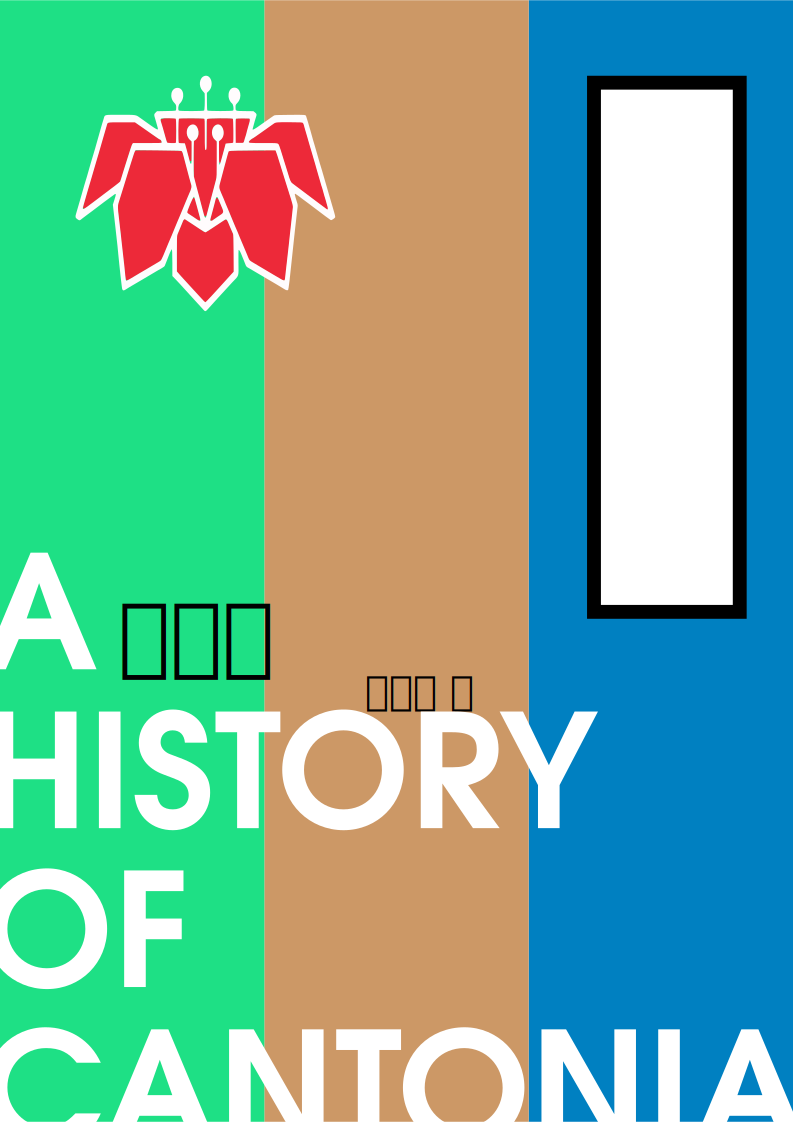
\includepdf{cantonia-history-cover.png}
	\blankpage
	

	\author{執經生}
	\title{南粵史}
	\date{2016}
	\pagenumbering{gobble}
	\maketitle
	
	\pagenumbering{roman}
	
\chapter*{序}

\begin{flushright}
	刘仲敬
\end{flushright}

\begin{quoted}
	上帝保佑南粤,南粤自由万岁。
\end{quoted}

南粤先民从记忆无法追溯的远古时期开始,就在韩江、珠江流域生生不息,为人类贡献了芋头、香蕉、西米和众多块茎食物,尤其是丰富多彩的亚热带水果。粤人得天独厚,享受伊甸园一样的美好生活,不太需要为觅食而终岁操劳,可以将大部分时间用于艺术创造。相形之下,黄河中游的鼠尾草食物就显得既乏味又单调。粤人陶醉于印纹陶器的几何形花样,在纹身艺术上精益求精,只能属于宽裕悠游的民族。黍米民族的艺术作品讲究单调实用,想象力的天花板甚低,折射出物主的艰难窘迫。

西南亚贸易线和南洋贸易线的发展,给南粤的富实锦上添花。犀角、象牙、玳瑁、明珠,养育了合浦的土豪和商人。粤人身为海上民族,是全世界的邻邦。他们的技术水平,远远高于闭塞的东亚内地。南粤先民以高超的冶炼技术、锐利的短剑和好勇轻生的武士精神著称。他们的原始丰饶比东亚内地各民族开始得更早,结束得更晚,仿佛天将降大任于斯人,保存了丰沛未凿的元气。粤人勇敢、骄傲、富裕,对自己的部族共同体非常满意,不屑于放弃自己的优越生活,模仿蚂蚁一样卑微的北佬官吏和士兵。

装腔作势的帝国朝廷往往声称普天之下莫非王土,在地图和文书上管理南粤。然而在南粤的土豪和武士眼中,朝廷的官吏无异于打秋风的浪人。他们长途跋涉的主要动机,不外乎觊觎黄金海角的奇珍异宝,渴望满载而归的幸福时刻。他们如果知趣,南粤土豪通常不会吝惜珍珠。他们如果不知趣,就会将南粤武士的吼声留在断简残篇当中。南粤豪杰辈出,一再教育无理取闹的支那人,让他们懂得怎样尊重东道主的自由和习俗。

大航海时代为粤人打开了更加广阔的窗口,将东亚的伟大民族变成了世界的伟大民族。海洋民族一向胸怀宽广,擅长吸纳全世界的思想资源,不亚于经营东西洋的物资资源。儒家文化、印度文化、日本文化、伊斯兰文化和基督教文化都在南粤共同体成长的各个阶段,贡献了宝贵的组织模式和文化财富。随着世界体系的延伸,南粤民族也开始构建自己的国族。共铲国际在帝国解体的间隙期入侵东亚,同时造成了真空的解放效应和真空的填补效应。

共同体如果已经成熟,帝国的瓦解就是自我解放的机会窗口。波兰和芬兰就是这一类共同体的典范,已经具备承担责任的能力,一旦获得解放,就能顺利填补帝国解体留下的真空。列强只要能够找到负责任的交涉对象,就无需费力拼凑断肢残体。共同体如果尚未成熟,帝国的瓦解就会导致弗兰肯斯坦式假共同体的产生。弗兰肯斯坦是各种尸体碎块拼凑而成的假人,自然没有真人的生命力,但在真共同体发育不全的情况下,列强就只有用临时拼凑的假共同体填补帝国解体留下的真空。

塞尔维亚-克罗地亚-斯洛文尼亚联合王国(南斯拉夫王国)和汉满蒙回藏联省共和国(中华民国)就是典型的弗兰肯斯坦,当然没有真正生命体的自我保护能力。这就是为什么广土众民的南斯拉夫民族和中华民族在国际恐怖组织和颠覆势力面前不堪一击,而小小的克罗地亚民族和南粤民族却能奋斗自卫的根本原因。共同体无论多么弱小,都比原材料强大。生命无论多么弱小,都比死肉强大。

天命为腐肉准备了秃鹰,让communism为诸夏驱除。南粤永远得风气之先,《南粤史》自然应运而生。粤人每逢历史的节点,都不会缺乏天命的担纲者。国族通过民族史的编撰,发现了自己。民族史既是历史的纪录者,又是历史的驱动者。古老而又年轻的南粤民族一脚踢翻了楚门的世界,大开门户迎接久违的阳光和空气。


	
\chapter*{Mandarin版排版序}

这本书内容的版权属于身为作者的执经生前辈;封面则是我自己随手设计的。在决定做这次排版的时候,在网上连付费下载电子版的地方都找不到,唯一剩下的只有不知为何仍在某个fandom.com托管站点上的据说是第一稿的版本。原文似乎并非用粤语而是用当代Mandarin白话文写就而有个别字被替换成(此前未见,大概是前辈自己设计的)粤语罗马字;因为替换的质量并不好(举例而言,有些地方的「此」字则无视上下文尽数被转换成粤语「呢度」),这次就先尽量恢复原本的Mandarin白话文,以后若有机会,必定再用粤语重版。

\begin{flushright}
	Setsuna K the Cantonia Rogue \\
	二〇二三年夏於南粤故土,已經不復存在之都市
\end{flushright}
	
	\pagenumbering{gobble}
	\tableofcontents
	
	\pagenumbering{arabic}
	\mainmatter
	\part{上编·古代史(远古—1513) }
	\chapter{百越时代和第一次北属}

\section{百越人:自由的南粤先民}

三万年前,当现代东亚居民的祖先经缅甸进入东亚时,他们并未想到以后会发生如何的历史活剧。这些人分为两支,其中一支沿长江东下,占据了长江至黄河间广阔的土地。这一批人,是日后华夏的祖先。另一支人则沿西江东进,占据着西起南粤、东至吴越的沿海月牙形土地。他们提供了现代南粤人的大部分遗传基因,是我们南粤的伟大祖先:越人\footnote{徐承恩:《躁郁的城邦》,页30。}。

越人内部分为很多不同的部族,统称“百越”。越人先民拓殖这片沿海月牙形土地的历史无疑是漫长的,亦一定是伟大的。由于缺乏文字记载,我们没有办法了解这一伟大拓殖史的具体细节,但能通过分子人类学的研究勾勒出大致框架:越人首先在相当于今天广东、广西、越南北部的地域形成了南越、西瓯、雒越三族。同时,他们向着空旷无人的东北、正东两个方向不断迁移。东北一路,越人进入江右,形成干越族。其后,他们中的一部分人继续东进到吴越,形成于越族,在宁绍平原和太湖流域创造了辉煌的河姆渡文化\footnote{陈国强:《于越在历史上的贡献与地位》}。正东一路,越人入闽,形成了闽越各部。最后,在这两路越人的交汇点上,形成了位于今日温州一带的东瓯族\footnote{李辉:《百越遗传结构的一元二分迹象》;林蔚文:《中国百越民族经济史》}。在长江以南的地域,百越和湖湘的三苗、滇地的百濮一起构成了族群复杂的多彩世界。

在无文的上古,当中原的华夏先民正处在混沌蒙昧之中的时候,诸越已经创造了灿烂的文明。早在公元前一万年前后,在地中海东岸的人们开始栽培大麦和小麦的时候,三苗和南粤先民开始栽培水稻,形成了东亚最早的农业\footnote{徐承恩:《躁郁的城邦》,页32}。五千年前,当吴越的土地上兴起伟大的良渚文明的时候,粤北山区出现了成熟的农耕社会,南粤的海岸线上就出现了很多以渔猎和采集为生的居民。温暖潮湿的海岸线被这些先民提供了舒适的生活环境和充足美味的海鲜,他们驾驶着原始的木舟出没于海岛之间,用鱼网捞取食物。今天,我们只能通过分布在西起雷州、东至汕尾的漫长海岸线上的无数贝丘遗址凭吊他们曾经的故事\footnote{《广东通史》古代上册,页59}。一个个贝丘遗址中数量庞大的贝壳残留,表示他们的饮食相当健康,能够摄入充足的蛋白质。

与史前时代物质简陋、暴力嗜血的豫中小邦不同,百越人的文明有着低烈度的战争和高度精致的物质、精神生活。南粤各地史前遗址中出土的精致玉器,暗示着南粤先民同良渚文明间的相似\footnote{关于南粤史前遗址中出土的玉器,参见杨少祥等:《广东海丰县发现玉琮和青铜器》}。种类繁多的骨角牙雕器和玉石、水晶饰物则不但表明南粤先民有着远远高于北人的审美水平,亦暗示着先民们时常从事复杂的原始宗教活动\footnote{《广东通史》,页81、93}。爱美、爱和平和敬畏神明是他们的美好特点。这一切,无疑是建基于丰富的物质基础上的。

我们的祖先虽爱好和平,但绝不柔弱。约三千年前,南粤进入青铜时代,铜鼓成为了我们祖先的文明中十分重要的元素。在青铜时代,南粤先民们往往在部落的中心位置放置一面铜鼓。每当危急情况来临,铜鼓就会被敲响,骁勇的部落战士们随即被召集起来,头戴绚丽精致的羽冠,乘坐战船出征\footnote{可参看徐承恩《郁躁的城邦》,页32}。部落间的交战虽不似上古中原小邦间的战争那么残酷,却依然是战士们展现勇武的场所。各部落中没有强大的君权,战士们因为部落共同体而战的使命感和荣誉感将凝结在一起,一如塔西佗笔下的日耳曼初民武士\footnote{对于上古南粤之缺乏君权,参见《吕氏春秋》:“缚娄、阳禺、驩兜之国多无君。皆南粤之夷无君者。”见是书卷20}。

铜鼓文化的范围不仅涵盖了南粤,亦遍及整个东南亚\footnote{梁志明:《东南亚的青铜时代文化与古代铜鼓综述》,《南洋问题研究》2007年第4期}。这一点表明,南粤人从史前时代开始便通过南海和中南半岛、马来半岛、印度尼西亚、菲律宾进行交往。珠海宝境湾的出土岩画表明,在两千至三千年前,南粤先民已能建造船首高翘、有桅杆和船帆的海船。这表明早在无文的时代,自由的南粤先民便已驾驶着帆船航行在广阔的南海上航行\footnote{《广东通史》页135-137}。我们可以想像,在原始落后的技术条件下,他们的航行会有多么艰难。他们是南粤历史上最早的航海者,是无数不被史册记载的达伽马和麦哲伦。

热爱生活、敬畏神明、自由勇武、善于航海的南粤先民有着迥异于上古诸夏的习俗。和所有百越人一样,南粤先民喜食鱼、鳖、蛇、蚌、蛤,还有生食的习惯。在今天的粤菜中,这一特点依旧十分明显。在多雨潮湿的南粤,我们的祖先居住着流行于东南亚的“干阑”式建筑,搭木为屋,楼上居人,楼下饲养牲畜。上古华夏世界的居民们不能理解这种建筑形式,遂荒谬地称南粤人“巢居”。百越人断发椎髻和“雕题凿齿(文身拔牙)”的习俗,亦使南粤先民在外观上和华夏迥异。在遵行周礼的上古华夏世界看来,崇信巫鬼、“越巫”大行其道的百越世界更是令人难以理解的异域。最令北人畏惧的,则无疑是越人“习于水斗,便于用舟”的特性。华夏世界的车战在水网纵横的越土毫无用无之地,丧失了军事技术优势\footnote{《广东通史》页160—162}。很快,入侵南粤的暴秦侵略军将因此付出沉重的代价。

\section{最早的南粤国家:之侯、公师隅、高固}

公元前333年,楚威王的军队消灭越国,杀害了越君无疆。彼时,诸夏短暂的青春期已一去不返,处在文明盛夏的战国七雄相继变法,纷纷抛弃封建秩序、拥抱集权和总体战。而当时的南粤,却依然是一片自由的越人乐土。越国灭亡后,同为越人的无疆之子之侯逃到南粤,建立起了一个世外桃源般的国度。之侯的具体逃亡路线今已不可考,但能够确定的是,数千年以来吴越、闽越和南粤的越人之间一直维持着广泛的文化乃至人口交流,之侯入粤路线很可能早已有无数先民走过\footnote{《广东通史》页100}。之侯在南粤积极任用本地人处理政事,越人公师隅是他最信任的大臣之一。公元前314年,公师隅在珠江口建造了今日广州城的前身——南武城。随着广州的出现,一则动人的民族神话诞生了:据说,在广州筑城之前,珠江口一带发生了严重的饥荒,民不聊生。危急时刻,南海的空中突然传来优美的仙乐,在五彩祥云中,五名身着五色彩衣的仙人分别骑着五色仙羊从天而降,每只羊口中都衔着“一茎六出”的优质稻穗。仙人将稻穗赠与当地人后,腾空而去。从此,珠江口风调雨顺,成为南粤最富庶的地方,广州城在这里诞生。

这一和广州筑城有关的神话虽有着后世加工的道教色彩,但亦反映了南粤人的一些文明特征和观念。仙羊衔稻穗的故事情节,无疑和百越人先进的稻作文明有关\footnote{刘付靖:《百越民族稻谷起源神话与广州五羊传说新街》,《中南民族大学学报》第23卷第2期}。当上古诸夏的居民还在食用难以下咽的黍、粟时,我们的祖先已经能够享用美味的米饭了。而这一神话将广州称为南粤最富庶之地,又反映了我们的祖先在上古时代即已将广州当做南粤文明的中心。

对于和自己有亡国、杀父之仇的楚国,之侯怀有强烈的仇恨和警惕心理。公元前312年,之侯命公师隅出使魏国,以结成南北夹击楚国的同盟。在魏都大梁,公师隅的使团向魏襄王献上了由三百只船、大批箭支及犀角、象牙组成的丰厚礼物\footnote{“(隐王元年)四月,越使公师隅来,献舟三百、箭五百万及犀角、象牙。”见《竹书纪年注》卷下}。这批礼物不但表明当时的南粤不但有着不弱的军事实力,亦是一片物产丰饶、盛产珍宝的乐土。此后,我们未能在史籍中见到关于之侯政权的记载,亦未见到粤魏反楚同盟采取了何种联合行动。然而,公师隅的这次出使壮举表明,公元前4世纪的南粤已经拥有了和战国强国魏平起平坐的实力,实为当时东亚大陆上一股不容小觑的势力。

在之侯的王国于史籍中消失后,南粤又回到了没有君权的状态。百余年后秦军入侵南粤时,南粤并无一个强大的政权统领全粤进行抗战。事实上,之侯政权本身的集权程度很可能亦不会很强。据说在之侯入粤时,一位名叫高固的南粤人甚至去到之侯的敌国楚国担任丞相。在相楚的五年中,高固曾因楚威王不能尽读《左氏春秋》而进呈简短的《铎氏微》一书予楚王\footnote{胡守为:《岭南古史》,页23-24。关于《铎氏微》一书,司马迁有云:“铎椒为楚威王傅,为王不能尽观《春秋》,采取成败,卒四十章,为《铎氏微》。”见《史记》卷14《十二诸侯年表第二》。}。高固的经历表明,之侯对于南粤的控制力度似属有限,他甚至不能阻止粤人出仕楚国。另一方面,高固助楚王读《春秋》的故事则说明,彼时的南粤已有人能够阅读诸夏的典籍,南粤和华夏已产生了文化交流。

\section{越秦战争和第一次北属}


公元前221年,暴秦消灭六国,华夏世界进入历史的终结。此时,秦始皇的欲壑却仍未满足,他还想将他的帝国扩张得更大、征服疆界推进得更远。公元前215年,经过六年的准备,秦始皇派遣蒙恬进攻匈奴,令尉屠睢、赵佗入侵南粤\footnote{秦军发动入侵南粤战争的时间,学界说法不一,此处采用胡守为的说法。见胡守为:《岭南古史》,页25。}。五十万暴秦侵略军兵分五路,越五岭(都庞岭、萌渚岭、骑田岭、大庾岭、越城岭)而下,其最西两路首先击溃了西瓯族的抵抗,杀害西瓯君译吁宋。第二年,秦军已全面深入南粤腹地,在珠江口南武城之处、广西北部、越南和广西交界处分别设置了南海、桂林、象郡这三个殖民点。

这批秦军由“逋亡者、赘婿、贾人”组成,乃诸夏封建秩序解体的产物,带有浓烈的流氓无产者气息。秦始皇以这批人侵略南粤,性质和汉武帝令囚徒、寇盗和恶少入侵大宛相同,皆属于大一统帝国将社会矛盾向外转移的秘传心法。流氓无产者大军的纪律一定不会非常好,抢掠很可能是他们士气的主要来源。很快,他们的恶性便彻底激怒了南粤先民们。两万余年来,我们的祖先一直在自己的土地上享受着越人部落固有的古老自由。现在,当暴秦的战争机器在南粤的土地上肆虐时,我们的祖先怎会甘心成为新兴专制的奴隶?于是,一场捍卫家园和自由的伟大抗争爆发了。

在南粤的每一寸山河上,先民们躲进丛林中和秦军周旋。他们宁肯和野兽待在一起,亦要坚持抵抗,绝不做秦人的降虏。为了镇压这些伟大的抵抗者,秦军用尽了一切手段,“三年不解甲弛弩”,仍旧一筹莫展。在河流和群山之间,善于水战的先民们将一处处粤土变成了侵略军的坟场。为了补给日渐吃紧的南粤前线,暴秦不得不开凿了沟通长江流域和珠江流域的灵渠以运送补给,却仍不能挽回败局。经过三年的浴血战斗,南粤先民们终于迎来了胜利。对于这场胜利,史书上的记载惜墨如金。然而,从简短的文字中,我们依然能感受到这场胜利的辉煌、体会到这场胜利带给我们的荣耀:

\begin{quote}
	夜攻秦,大破之,杀尉屠睢,伏尸流血数十万\footnote{司马迁:《史记》卷52《平津侯主父列传第五十二》}。
\end{quote}

这是一场战果异常巨大的胜利,亦是南粤历史上第一次在抗击外敌的战争中获胜。无论我们用怎样美好的言辞赞美这场胜利,都无法描绘那些南粤战士们的伟大。侵略军主将屠睢被他们击毙了、数十万侵略者命丧南粤。和这场战争时隔两千余年的我们在重温这段历史时,依然能够无比地感动、无比地骄傲。这是古老自由对新兴专制的胜利、是南粤对帝国的胜利。它将永载史册,成为南粤不朽的光荣。

屠睢死后,他的副手赵佗接替了他的位置。暴秦明白,单靠屠杀和镇压是绝无可能成功统治南粤的。于是,大规模的殖民运动开始了,五十万“谪徙民”被暴秦派往南粤“和越杂处”。由于许多在粤殖民者无妻,赵佗向秦始皇请求派遣三万女子南下,而秦始皇却仅派遣了一万五千人\footnote{司马迁:《史记》卷118《淮南衡山列传第五十》}。殖民者中严重失调的男女比例使他们中的许多人只得娶越人女子为妻。在赵佗的主持下,屠杀政策停止了,南粤先民们和殖民者间维持着和平的关系。赵佗由一个侵略军将领转变成了哥伦布式的殖民地经营者。随着通婚规模的扩大、越人女子及殖民者男子的子女不断出生,殖民者们日渐浸淫在南粤本土文化中,变得日益越化,融入了南粤本土的共同体当中。今天,这批殖民者为现代10\%的南粤男性提供了Y染色体\footnote{徐舜杰、李辉:《岭南民族源流史》}。

然而,此时的赵佗仍未忘记自己是一名秦军将领,他仍要为暴秦开疆拓土。他将阴鸷的目光瞄向了更南面。在那里,有一个名叫雒越国的国家。

\section{瓯雒国的灭亡}

瓯雒国位于今天的越南北部,是一个和古蜀文明关系极深的国度。公元前316年,暴秦灭蜀,古蜀末代君主开明十二世殉国\footnote{秦灭蜀之时间,史家有不同说法,此处采取流传最广的公元前316年说。}。古蜀遗民逃亡滇中,又经红河东下。公元前257年,他们在古蜀王族泮的带领下到达越南北部的红河平原。据说,当时红河平原上的雒越族已有了一个名叫“文郎国”的国家,其首领的称号为“雄王”。雄王绝非集权君主,而是一个典型的部落联盟首领。在雄王之下,被称为“雒侯”、“雒将”的酋长依靠百越的自由传统统率着各部落\footnote{郭振铎、张笑梅:《越南通史》,页122。}。据传说,蛮勇并耽于酒食的雄王因“不修武备”而被泮的军队击败、赴井而死。泮自称安阳王,筑古螺城,在红河平原建立了由古蜀人统治的瓯雒国\footnote{陈重金:《越南通史》,页18。}。

古蜀遗民之所以能顺利到达红河平原,系拜上古巴蜀夜郎——安南印度间的贸易路线所赐。巴蜀夜郎被帝国吞灭后,史后之人已无法相像这条路线的存在。日后的越南阮朝史臣修史时,看到这段古史觉得难以置信,只好认为这些古蜀遗民其实是越南北部一个由蜀姓酋长率领的部落\footnote{阮朝史臣称:“蜀自周慎靓王五年已为秦所灭,安得复有王者……相隔二三千里,蜀安得远跨诸国而跨交郎乎……或者西北徼外与文郎邻有姓蜀者,遂以为蜀王,亦未可知。谓蜀王、又巴蜀人,则非矣。”引自《钦定越史通鉴纲目》卷1,页8。此段文字,实为史后之人史观的绝佳案例。}。然而,对越南北部红河流域东山文化遗址的考古发掘已经证实,该文化所用的陶器、青铜器和古蜀文明极为相似\footnote{张弘:《先秦时期古蜀与东南亚、南亚的经济文化交流》,《中华文化论坛》2009年第1期,页129—131。}。由此可见,古蜀遗民在越南北部建立瓯雒国的历史记载是颇有可信度的。

瓯雒国的国名暗示着安阳王治下不但生活着雒越人,亦有部分西瓯人,该国的控制区很可能深入今日的广西境内。安阳王手下的“强兵勇将”有三万之众,其军事实力无疑高于文郎国\footnote{郭振铎、张笑梅:《越南通史》,页132。}。于此同时,红河平原上“雒侯”、“雒将”的权力亦未遭到破坏。古蜀遗民作为征服者,很有可能将红河平原变为了混合蜀越宪制的区域,一如丹麦人入侵英国后制造的格局。 

公元前207年,赵佗发动了对瓯雒国的入侵。对于这场战争的进程,史书进行了神话式的记载:传说,早在安阳王筑古螺城时,曾获得一只金龟的帮助。金龟离去时,脱爪一只赠予安阳王,以助其抵御外侮。安阳王以龟爪为弩机,造出了一部名为“灵光金爪神弩”的武器。赵佗军来攻时,安阳王以神弩抵抗,“三放杀三万人”。赵佗见强攻失利,遂和安阳王议和,送其子赵仲始于雒越国中为人质。很快,安阳王的女儿媚珠和“风姿闲美”的赵仲始便坠入了爱河\footnote{《钦定越史通鉴纲目》卷1,页18。}。在赵仲始的诱惑下,媚珠鬼迷心窍地带他查看了神弩。其后,赵仲始偷走了金龟神爪,并托以省亲为名北归。失去了神弩庇护的安阳王再也不能保护自己的国家。在赵佗军的又一次入侵下,瓯雒国灭亡了\footnote{陈重金:《越南通史》,页133。}。

赵仲始和媚珠的爱情故事,则有一个凄美的结局。赵仲始北归之前曾问媚珠:“异日我再来,万一两国失和,当作何等验质可见?”媚珠答道:“妾有鹅毛绵褥,常以附身。所至歧路,拔鹅毛识之,可知妾所在。”古螺城破后,安阳王乘马载媚珠南逃至海滨,走投无路,遂在拔剑斩杀媚珠后投海殉国。稍后,跟随鹅毛踪迹领追兵赶到海边的赵仲始只见到了媚珠的尸体,伤心欲绝,便带着媚珠之尸回到古螺城,投井自尽\footnote{《钦定越史通鉴纲目》卷1。}。

这一神话中,安阳王筑城得金龟之助的故事,和秦军灭蜀后筑成都时得到神龟帮助的传说非常像,无疑暗示了瓯雒国的古蜀渊源\footnote{关于成都筑城与龟之间的关系,可参看王文才:《成都城坊考(上)》,《四川师范学报》(社会科学版)1981年第1期,页58—66。}。安阳王拥有令赵佗畏惧的神弩,则似在暗示古蜀人的技术水平要比赵佗麾下的秦军高一个档次,而这种技术差距极有可能是由印度安南——夜郎巴蜀这条通道输入的。赵佗以卑鄙手段破坏神弩,无疑象征着暴秦的凶残和狡诈。媚珠和赵仲始的悲惨结局,更给瓯雒国和古蜀文明的最后灭亡抹上了浓重的悲剧色彩。虎狼之秦惩其凶焰,在南粤和越南的土地上演了其第二次灭亡大蜀的暴行。

然而,赵佗毕竟不是屠睢。消灭瓯雒国后,雒侯、雒将们固有的地位、雒越人固有的自由和共同体并未遭到破坏。此时秦始皇已死,由陈胜吴广掀起的滔天洪水在秦帝国的核心领土上肆虐。赵佗就如同英国历史上那些失去欧陆领土的诺曼武士后代一样,坚定地走着本土化的道路。一年后,他将在南粤大地上创造惊人的伟业、开创一个伟大的南粤国家。

	
	\chapter{伟大的南越国}

\section{南越国的建立}

\indent 公元前206年,暴秦灭亡,席卷华夏世界的第一次大洪水却仍未终止。在南粤,赵佗处在历史的十字路口上:究竟是将南粤变为“天下”的一部分、加入到在洪水中瓜分暴秦尸体的争霸战争中,还是让南粤自立、使她免遭洪水的侵害?
当时,赵佗的官职是龙川令,管辖着秦南海郡东部重镇龙川县。而在南粤掌握军政大权之人,则是南海尉任嚣。暴秦令“战功赫赫”的赵佗屈居于任嚣之下,不知是否有借任嚣防范赵佗之意。若有的话,暴秦无疑是失算了。其时任嚣已是重病将死之人,自知时日无多的他将赵佗召至南海郡城番禺,说了如下一番推心置腹的话:

\begin{quote}
	闻陈胜等作乱,秦为无道,天下苦之。项羽、刘季、陈胜、吴广等州郡各共兴军聚众,虎争天下,中国扰乱,未知所安,豪杰畔秦相立。南海僻远,吾恐盗兵侵地至此,吾欲兴兵绝新道,自备,待诸侯变,会病甚。且番禺负山险,阻南海,东西数千里,颇有中国人相辅,此亦一州之主也,可以立国。郡中长吏无足与言者,故召公告之\footnote{ 司马迁:《史记》卷113《南越列传》}。
\end{quote}

此段说话中,任嚣点出了南粤背靠南岭、面朝南海、东西数千里、足以自守的地利,希望赵佗依靠暴秦留下的武力自立,避免大洪水波及南粤。不久后,任嚣将南海尉之职交予赵佗,驾鹤西去。赵佗果然没有辜负任嚣的嘱托,他立即向粤北的横浦、阳山、湟溪关发出了一道简短的命令:

\begin{quote}
	盗兵且至,急绝道聚兵自守\footnote{司马迁:《史记》卷113《南越列传》}!
\end{quote}

在这里,赵佗将岭北流窜至粤的散兵游勇称作“盗兵”,要求南岭各关口断绝道路,以兵自守。南粤终于结束了第一次北属,与岭北决裂了。

其后,赵佗挥军从南海出发,对桂林、象郡展开了疾风烈火般的攻击,两地的暴秦长吏纷纷被击毙,赵佗的部下接管了整个南粤。三年后,公元前203年,出生于赵国真定的赵佗自称南越武王,采取“与辑百越”的政策,自己亦完全采纳了百越人的礼仪、发式与饮食习惯,成为了归化越人。至此,一个强有力的南粤本土国家、伟大的南越国,在南海与南岭之间出现了!

\section{永远的英雄:南越武帝}

\indent 公元前202年,项羽在奋战后消失于巫江畔的乱军之中,华夏世界重返封建体系的努力失败,继承暴秦遗产的汉帝国出现。在大一统史观的叙事体系下,从公元前202年开始,东亚大陆进入了汉代。然而,只要我们将目光移向与西汉初年同时的百越之地,就会明白实际情况其实远更复杂。

在吴越南端,东瓯王摇统治着东瓯族国家东瓯国。在八闽之地,闽越王无诸控制着强大的闽越族国家闽越国。今天广东、江西、福建的交界处,也就是日后客家人的聚居区,闽越国南武侯织于公元前195年被汉朝册封为“南海王”,建立了南海国。这些国家与南越国一起,在百越之地构成了一片连续的越人国家。至于南粤以西,在今天被称为“西南”的区域,则有夜郎、靡莫、滇、卭都等被汉人统称为“西南夷”的独立王国或者部族联盟。所有这些政权一同构成了复杂的多国体系,从东南、南、西南三个方向以弧形包围了汉帝国南疆。与乏味单调的大一统帝国相比,此种多国体系无疑能够催生更复杂的宪制与国际关系,拥有更宽广的历史路径。因此,南越国一方面要考虑与汉帝国的关系,另一方面又要处理其它周边政权的关系。在这样复杂的国际舞台上,南越武王赵佗开始了保卫南粤的奋斗。

公元前196年,已将异姓王消灭殆尽、时日无多的汉高祖刘邦将贪婪的目光瞄向了尚未臣服于他的南越国。这一年,他派遣大夫陆贾出使南越,“册封”南越武王为“南越王”。为了南粤的和平及对汉通商之利,南越武王选择了接受“册封”,将南越国变为汉帝国名义上的藩属国。这绝不是卑躬屈膝的行为,仅仅是南越武王为对付汉帝国的威胁而采取的权宜之计。一旦汉帝国威胁到南越国的生存,南越武王一定会毫不犹豫地与之战斗到底。不久后发生的事情,即说明了这一点。

公元前183年春,汉帝国的实际掌权者吕后实行了“别异蛮夷”政策,禁止对南越国出口金铁、田器、母马、母牛、母羊、母畜。汉帝国背信弃义、擅自挑起争端的行为令武王感到由衷愤怒,他先后派遣内史藩、中尉高、御史平三名高官出使长安,对汉廷据理力争\footnote{ 梁廷柟:《南越五主传》,页7—8}。然而,吕后却卑鄙地扣留了三名使者,继续推行“别异蛮夷”政策。武王明白,辩论已经无效。能够捍卫南粤的方法,只有战斗一途。他直接指出了汉帝国吞灭南越国的狼子野心:

\begin{quote}
	别异蛮夷,隔绝器物,此必长沙王计也,欲倚中国,击灭南越而并亡之,自为功也\footnote{司马迁:《史记》卷113《南越列传》}。
\end{quote}

长沙国系汉朝分封于湖湘的异姓王国,其王室吴氏是刘邦异姓王大清洗中的唯一幸存者。长沙国对汉帝国的忠诚,由此可见。为保卫南粤而决意一战的武王立即自称“南越武帝”,发兵北伐长沙国,破其数邑。南越国与汉帝国之间,至此进入战争状态。

面对南越国的反抗,汉帝国露出了极度凶残的面目。残忍的吕后令人屠杀了武帝留在北方的几乎所有亲属,并捣毁了武帝父母的坟墓\footnote{ 张荣芳:《南越国史》,页193。}。公元前181年9月,一支庞大的汉帝国侵略军在隆虑侯周灶的指挥下抵达南岭,准备彻底消灭南越国。在武帝的指挥下,南越子弟兵同仇敌忾地坚守南岭各关口,“据险筑城”,令侵略军“兵不能逾岭”,只得退守长沙。在长时间的僵持中,越化的南越军完全能够适应湿热的气候,北人组成的汉军则饱受疫病折磨。经一年多的对峙,公元前179年,吕后病死,汉帝国侵略军狼狈北撤\footnote{ 张荣芳:《南越国史》,页195。}。在南越武帝的指挥下,不屈的南粤赢得了第二次抗击外敌的伟大胜利。越汉战争的胜利令南越国声威大震,成为汉帝国以南的一流强国。这时,不但西瓯、雒越人臣服于南越国的统治下,就连闽越、夜郎等国亦慑于南越国的兵威与财力,成为南越的臣属\footnote{ 张荣芳、黄淼章:《南越国史》,页156—158。}。这时,南越国的领土与属国的疆域已有“东西万余里”,南越武帝更是“乘黄屋左纛,称制,与中国侔”,南越国成为了足可与汉帝国相提并论的超强国家\footnote{ 司马迁:《史记》卷113《南越列传》}!

色厉内荏的汉帝国见武力无法征服南越国,遂决定采取怀柔政策。在汉军北撤的同一年,汉文帝在武帝的家乡河北真定寻访到了武帝残存的堂兄弟,给予官爵。同时,汉文帝还派人为武帝在真定的祖坟“置守邑,岁时奉祀”,并派遣曾出使过南越国的太中大夫的陆贾再次出使南越\footnote{ 司马迁:《史记》卷113《南越列传》}。陆贾到达南越后,武帝携他遍游国中名胜,并将一封书信交给陆贾,让其带回长安。这封书信充分展示了武帝为保卫南粤而展现出的高超外交智慧,值得全文引用:

\begin{quote}
	蛮夷大长老臣佗昧死再拜上书皇帝陛下:老夫故粤吏也,高皇帝幸赐臣佗玺,以为南粤王,使为外臣,时内贡职。孝惠皇帝即位,义不忍绝,所以赐老夫者厚甚。高后自临用事,近细士,信谗臣,别异蛮夷,出令曰:“毋予蛮夷外粤金铁田器;马、牛、羊即予,予牡,毋与牝。”老夫处辟,马、羊、羊齿已长,自以祭祀不修,有死罪,使内史藩、中尉高、御史平凡三辈上书谢过,皆不反。又风闻老夫父母坟墓已坏削,兄弟宗族已诛论。吏相与议曰:“今内不得振于汉,外亡以自高异。”故更号为帝,自帝其国,非敢有害于天下也。高皇后闻之大怒,削去南粤之籍,使使不通。老夫窃疑长沙王谗臣,故敢发兵以伐其边。且南方卑湿,蛮夷中西有西瓯,其众半羸,南面称王;东有闽粤,其众数千人,亦称王;西北有长沙,其半蛮夷,亦称王。老夫故敢妄窃帝号,聊以自娱。老夫身定百邑之地,东西南北数千万里,带甲百万有余,然北面而臣事汉,何也?不敢背先人之故。老夫处粤四十九年,于今抱孙焉。然夙兴夜寐,寝不安席,食不甘味,目不视靡曼之色,耳不听钟鼓之音者,以不得事汉也。今陛下幸哀怜,复故号,通使汉如故,老夫死骨不腐,改号不敢为帝矣!谨北面因使者献白璧一双,翠鸟千,犀角十,紫贝五百,桂蠹一器,生翠四十双,孔雀二双。昧死再拜,以闻皇帝陛下\footnote{ 班固:《汉书》卷95《西南夷两粤朝鲜传》。赵佗之自称,原文作“蛮夷大长老夫臣佗”,殊难解。据胡守为考证,“夫”似为衍文,当作“蛮夷大长老臣佗”,今据胡氏之考证改。参见胡守为:《岭南古史》页38—39。}。
\end{quote}

书信中,武帝自称“蛮夷大长老”,充分展现了他以南粤为家,自认为本土“蛮夷”的自我认同。武帝的用词看似卑下,实则处处声讨着汉帝国的不义:正是汉帝国采取“别异蛮夷”政策、扣押南越使臣破坏了越汉之间曾经友好的关系,武帝称帝于番禺则更是反击汉帝国杀害其家人、掘毁其先人坟墓的正义之举。接下来,武帝又将挑起两国战争的责任推到汉帝国属国长沙国的头上,暗示汉文帝越汉之间仍有谈判余地。至于武帝乞求汉帝国给予封号的文字,正如日后的许多越南皇帝在一次次击退中华帝国的侵略大军后仍向帝国乞封一样,无疑是权宜之计,目的是为了避免战争长期化并导致祖国不得安宁。毕竟,外强中干的中华帝国十分容易满足于“万国来朝”的虚名。武帝乞封乃是在吃准了汉帝国的弱点后针锋相对地采用的巧妙护国策略,充满了在帝国威胁下保卫南粤的政治智慧。在书信最后一段,武帝称“老夫身定百邑之地,东西南北数千万里,带甲百万有余”,无疑是在向汉帝国表明:如果你们想把战争进行下去,南越国有实力奉陪到底。值得注意的是,武帝指出在南越国治下的西瓯人仍有自己的王。这表明南越国是尊重百越各族群习惯法与政治共同体的,绝不是碾平一切的大一统吏治国家。

我们不知道汉文帝在看到这封书信时是何种表情。可以推测的是,他的内心应该是无可奈何的。于是,南越国与汉帝国恢复了和平,武帝对外宣布“去帝制、黄屋左纛”,并对汉称臣。公元前156年,汉文帝死,汉景帝继位。在汉景帝朝,南越国曾有遣使赴汉“朝请”之举。当然,这一切不过是欺骗汉帝国、并使汉帝国自欺欺人地沉浸在“南越臣服”的幻象中的伪装。在南越国中,武帝一如既往地自称皇帝\footnote{司马迁:《史记》卷113《南越列传》}。南越国的这一政策,与日后越南人对付中华帝国的策略可谓如出一辙。

公元前137年,南越武帝驾崩,结束了他长达120年的波澜壮阔的人生,亦离开了他守护了67年的南粤。南越武帝人生的前后半段可谓截然两分。在前半生,他作为被暴秦灭亡了祖国的赵人降虏,为暴秦卖命,率领暴秦侵略军屠杀南粤百姓,并代表暴秦第二次灭亡了古蜀人的国家。然而,在洪水滔天的历史节点,他终于做出了正义的决断,毅然与帝国与自己的过去切割,使自己与数十万南下殖民者归化为越人,以南粤为家,建立了伟大的南越国。在后半生,武帝不但在礼仪、习俗上全面越化,亦为了保卫南粤殚精竭虑、不停奋斗。当汉帝国威胁到南越国的生存时,他更是毅然举兵北上,纵然自己留在北地的家人遭到汉帝国屠杀、先人坟墓被汉帝国掘毁,也要保卫南粤的自由。他后半生高尚的政治德性使他成为南粤史上的伟人之一,亦使他成为激励南粤人为自由而战的精神象征。他120岁的高寿则似乎在暗示,德性充沛的人一定会得到上天的奖赏。

\section{自立与归汉:文帝、明王、哀王朝的宪制斗争}

\indent 南越武帝赵佗以120岁高龄去世,他的继承人南越文帝赵眜是他的孙子,据说还是那位在古螺城殉情的赵仲始之子。在历史上,文帝的存在感远不如武帝强烈。然而,今天的我们仍能通过一处庞大的历史遗迹直观地体会到他曾经的存在,那便是著名的广州南越王墓。

公元1983年,一支工程队挖开了广州越秀区一座海拔不足50米的小山象岗山,一座大型陵墓出现在人们眼前。在用起重机打开两扇巨大的石门后,埋葬南越文帝的地宫在经历了2100余年的岁月后重见天日。地宫中出土的种种陪葬品足以令人震惊:十余件结构复杂、百越特色鲜明的铜熏炉骄傲地展示着南越国现金的铸造技术;九件铜提筒上装饰着各色花纹,其中一件上雕刻着四艘首尾相衔的羽人船,每船有羽人五名,有的在划桨、有的手持兵器、有的在杀人,展现着南越国军人杀俘祭海神的场景,反映了越人的虔诚与武德。七百余件铁器及一副铁制铠甲,表明当时的南越国已在大规模使用铁器。至于包裹文帝遗体的精美的丝缕玉衣,共由2300枚玉篇连缀而成,比西汉中山靖王刘胜墓中那件有名的金缕玉衣还要早十二年。最令人惊叹的,则是一件闪闪发光、由波斯舶来、盛放着十粒来自两河流域的药丸的银盒,以及五支长达1.2米的非洲象象\footnote{ 关于南越王墓出土文物的情形,参见张荣芳、黄淼章:《南越国史》,页376—388。}牙……这些陪葬品显示,南越国不但十分越化,更是一个重视海洋、海外贸易发达的国家。

对于南粤而言,南岭用以是抵御岭北帝国的坚固城墙,南海则是广阔的大后方。如前所述,早在史前时代,南粤的百越先民们便已驾驶着海船驰骋于南海波涛中。在南越国时代,南粤的海外贸易十分繁盛,来自波斯、两河流域、东非、东南亚的商品萃聚于番禺城,南越国人频繁地往来于东南亚及南海诸岛之间\footnote{ 张荣芳、黄淼章:《南越国史》,页314—315。}。究竟应当依托南岭、面向大海、建立一个自由的南粤,还是依附于大一统的汉帝国?围绕这一根本宪制问题而进行的政治斗争,是武帝去世后南越国政治史的主线。

文帝继位的第三年,即公元前135年,南越属国闽越乘武帝新丧之机发兵攻打南越的边境城邑。文帝缺乏武帝的果断,担心若南越国擅自发兵抵抗将触怒汉帝国,竟上疏汉廷求援。其时,汉朝的皇帝是刚刚上台四年的汉武帝。年轻的汉武帝就此获得了干涉越人内部事务的借口,因而对南越的“恭顺”大喜过望。在汉武帝的命令下,汉军从会稽、豫章两路出发,进攻闽越。同时,汉使唐蒙前往南越,将出兵的消息告知文帝。在南越国中,接待唐蒙的南越人为其准备了丰盛的食物,其中包括由巴蜀进口的枸酱。可是,南粤的热情好客却引来汉帝国居心叵测的暗算:唐蒙不怀好意地询问接待者枸酱产自何地,接待者直率地答称此酱系由西北方顺牂牁江(西江)而来。回到长安后,唐蒙经一番调查,发现牂牁江上游的南越属国夜郎实为蜀越枸酱贸易的中转站。于是,一个卑劣的计划在唐蒙心中浮现,他向汉武帝上疏称:

\begin{quote}
	南越王黄屋左纛,地东西万余里,名为外臣,实一州主也。今以长沙、豫章往,水道多绝,难行。窃闻夜郎所有精兵,可得十余万,浮船牂柯江,出其不意,此制越一奇也。诚以汉之强,巴蜀之饶,通夜郎道,为置吏,易甚\footnote{ 司马迁:《史记》卷116《西南夷列传》}。
\end{quote}

此一计划的要点在于:汉帝国不由正面进攻难以翻越的五岭,而应先制服越国西侧的夜郎,再由此顺江而下压制南越。在南越文帝对汉帝国毫无敌意,视之为盟友时,汉帝国居然仍在处心积虑地思考灭亡南越的计策。汉帝国之卑鄙无耻,于此可见一斑。汉武帝立即同意了唐蒙的提议,任其为中郎将,命他“将千人、赉食量及衣重者万余人”由巴蜀入夜郎,以贿赂手段收买了夜郎侯多同及当地各部落,并以夜郎之地为犍为郡\footnote{ 梁廷柟:《南越五主传》,页28。}。南越从此失去了西侧的藩篱。

出人意料的是,汉军尚未逾岭,闽越王郢即被其弟馀善发动政变杀害。其后,馀善无耻地将郢的头颅献给汉军,宣告投降,汉帝国不废一兵一卒即控制了闽越。为分化闽越,汉武帝立无渚子孙丑为“越繇王,奉闽越先祭祀”,又以卖国者馀善为东越王,“与繇王并处”\footnote{ 司马迁:《史记》卷114《东越列传》}。自此,南越又失去了东侧的藩篱。

在这之后,汉武帝的野心仍未满足。他派遣中大夫严助“以处分闽越事谕意南越”。面对汉使严助,南越文帝张惶无措,说出了如下一番丧权辱国的话:

\begin{quote}
天子乃为臣兴兵诛闽越,臣死无法报德……国新被寇,使者行矣,眜方日夜束装,入见天子\footnote{梁廷柟:《南越五主传》,页18。传统文献将文帝之名误作“赵胡”,此段记载原文为“胡方日夜束装”。然据南越王墓考古材料,文帝之名实为“赵眜”,乃于引文中改“胡”为“眜”。}。
\end{quote}

严助北去后,文帝的大臣们对于他轻易许下亲自“朝见”汉武帝的承诺感到震惊与愤怒。他们争相劝谏,指出如果文帝亲自入长安,将很可能被汉廷扣留、无法回国\footnote{梁廷柟:《南越五主传》,页18。}。毕竟,武帝时代吕后扣押三名南越使者的教训如在昨日,汉帝国糟糕的政治德性使南粤不可能相信其任何承诺。在群臣的劝谏下,文帝终于改变了主意,对汉帝国“称病,竟不入见。”然而,此前文帝对汉使严助屈辱的承诺已覆水难收,他的太子赵婴齐仍不得不赴长安“入宿卫”\footnote{司马迁:《史记》卷113《南越列传》}。这一举动,实为二十四年后南越国灭亡的导火索。

除了软弱地在汉使面前进退失据外,文帝并未在政治史上留下太多痕迹。公元前122年,文帝驾崩,结束了他并不光彩的一生。然而,南越国的苦难至此才刚刚开始。从长安回到南粤继承帝位的赵婴齐削去帝号,库藏了南越皇帝的玉玺,是为南越明王。明王卑微的态度使汉帝国自此“益易事南越”,屡次遣使敦促明王“入朝”,欲以此将他扣留在长安。明王明白自己若随汉使北上,定然有去无回,因此效仿文帝称病,“坚不肯入见”。不过,懦弱的他还是派出了王子赵次公入长安“宿卫”,一如文帝当年软弱地将他派往长安。更令人悲愤的是,明王不但在外交上继承文帝的卖国路线,在内政上更是任意妄为、疯狂地破坏南越国的法统。“乐擅杀生”的明王是一个残暴任性的君主。早年在长安时,他曾娶河北邯郸女子樛氏,生子赵兴。回到南粤后,他悍然不顾武帝制定的与越人通婚的政策,竟立樛氏为后,立赵兴为太子,全然不理他与越人王妃所生的长子赵建德\footnote{梁廷柟:《南越五主传》,页20。}。大概是因为明王过于残暴自恣,群臣无法阻止起有效的反对。公元前115年,明王病死,结束了他短暂而荒唐的统治。赵兴继位,是为南越哀王。因哀王年幼,樛氏居然获得太后身份、成为了南越国的实际掌权者。此时,南越国的法统已被明王破坏殆尽。

做为一名对南越国毫无认同感的北人,樛氏对南粤毫无感情,一心希望举南粤之地尽归汉朝。她力劝哀王出卖自己的国家、依附汉帝国。汉武帝闻知南越国中樛氏掌权、哀王年少的消息后,大喜过望。公元前113年,汉武帝令樛氏在北方的旧情人安国少季率使团出使南越国,要求樛氏、哀王“入朝,比内诸侯”\footnote{司马迁:《史记》卷113《南越列传》}。同时,汉卫尉路博德屯兵桂阳,以武力威胁做为安国少季的后盾。安国少季一到番禺,早已饥渴难耐的樛氏便与他厮混在一起。很快,两人便达成了两项彻彻底底的卖国协议:1)南越国如汉帝国“内诸侯”,三年一朝;2)解除边关防御。汉武帝迅速批准了这一协议,并增添了附加条款:3)“赐”南越丞相吕嘉银印,及内史、中尉、太傅印;4)废南越法,除黥劓刑,改用汉法;5)汉使留于南越国内“镇抚”。对于这些更为屈辱的条款,樛氏不但没有任何反对,反而高高兴兴地接受了它们。樛氏与哀王更开始整饬行装,为“入朝”汉武帝做准备\footnote{司马迁:《史记》卷113《南越列传》}。至此,南越国已经沦为与长沙国一样的地位,失去了一切的自主能力,几乎等同于被汉帝国吞并。

南越国最危险的时刻,到来了。

\section{南粤的大宪章运动:吕嘉革命}

\indent 在祖国马上就要灭亡的情况下,一个男子为了挽救南粤的自由站了出来,他就是南越国丞相吕嘉。

吕嘉是越人,自武帝时代起便已为官。在文帝、明王、哀王三朝,他都担任丞相。他的家族中官至长吏者达七十余人,男子皆娶王室女子,女子则尽嫁王族。在越人当中,吕嘉丞相有着极高的威望\footnote{司马迁:《史记》卷113《南越列传》}。面对樛氏与哀王肆意践踏南越武帝开创的伟大国度、面对祖国的沦亡,吕嘉感到出离愤怒。在哀王数次拒绝了他的劝谏后,他决心起兵反抗,继承南越武帝的遗志,为南粤的自由战斗到底。为了麻痹汉帝国,吕嘉首先称病不出,拒绝与汉使相见。汉使、樛氏、哀王对吕嘉的异动皆有所察觉,狠毒的樛氏遂计划借汉使之手杀害他。

为杀吕嘉,太后与哀王于宫中置酒,邀请汉使及群臣入宫赴宴,计划在宴会中下毒手。时为南越国之将的吕嘉之弟察觉到了危险,在吕嘉入宫后率兵驻于宫外。宴会开始后,樛氏不怀好意地对吕嘉说:“南越内属,国之利也,而相君苦不便行,何也?”意图以此语激怒汉使。正在汉使迟疑之间,警觉的吕嘉已察觉到了危险,起身急走而出。樛氏气急败坏,亲自持矛欲刺吕嘉,却被尚存良知的哀王阻止,吕嘉得以顺利逃出宫门与其弟的军队会合,率军回到家中。

此时,南越国群臣与百姓对于樛氏、哀王无耻卖国行径的不满终于爆发了。他们纷纷支持吕嘉丞相,几乎无人愿意听从那个与汉使安国少季私通的北人太后。番禺城中,困守王宫的汉使、樛氏与哀王已被宫外愤怒的南越爱国者们彻底包围,如同坐困于孤岛上一般。走投无路的樛氏欲下达杀害吕嘉的命令,却根本无人执行\footnote{司马迁:《史记》卷113《南越列传》}。

闻知樛氏与哀王已被支持吕嘉的官民困于宫中,汉武帝决定派出一支小部队越过边境以进行威慑。在汉武帝的命令下,汉济北相韩千秋及樛氏之弟樛乐统率两千人马跨过了边境。汉武帝失算了,他彻底低估了南粤人为自由而战的意志,更不知他面对的是一个怎样坚韧的国度。在汉军入境的刺激下,番禺城中南越国官民们的怒火彻底喷发了,一场由吕嘉丞相指挥的伟大革命开始了。吕嘉丞相决定武力进攻王宫,并发布了檄文:

\begin{quote}
	王年少,太后中国人也,又与使者乱,专欲内属,尽持先王宝器入献天子以自媚。多从人,行至长安,虏卖以为僮仆。取自脱一时之利,无顾赵氏社稷,为万世虑计之意\footnote{司马迁:《史记》卷113《南越列传》}。
\end{quote}

檄文中,吕嘉丞相列举了樛氏对南越国犯下的不可饶恕的罪行:首先,身为“中国人”的她把持朝政,与汉使私通,一意卖国投降,甚至为了讨好汉朝皇帝而将历代先王的宝器献出。其次,她还将南粤人贩卖到长安去做汉人的僮仆,做着人口贩子的生意。如此只顾一己之利的无耻行为,是一定会毁掉南越国的。为了南越武帝开创的伟大事业、为了南粤的自由,樛氏必须死。这一慷慨激昂的檄文,可称得上是有史以来第一篇南粤自立宣言。

在南越官民的支持下,吕嘉丞相的革命军攻入宫中,杀死了樛氏与哀王、杀光了汉帝国使团。吕嘉革命胜利了、南粤胜利了,文帝朝以来媚北归汉的外交路线被一扫而空,南粤回到了越人手中。 这场革命之于南粤的意义堪比大宪章运动之于英国的意义,足以证明面对北来僭主的威胁,南粤本土的志士们绝不会屈服,而是会反抗到底,保卫家邦,正如吕嘉丞相与南越国官民们所做的那样。


\section{南越国的灭亡}

\indent 吕嘉革命胜利后,由越人王妃所生、时为术阳侯的赵建德被立为王。此时,韩千秋、樛乐率领的两千汉军已攻破数城,正向南越都城番禺逼近。吕嘉丞相采取诱敌深入之策,将这股侵略者诱至番禺城附近全部消灭,侵略军头目韩千秋、樛乐皆被击毙。然而,这场小胜并不能左右大局,真正的考验尚未到来。闻知败报的汉武帝下令展开动员,欲以大军消灭南越国。在诏令中,汉武帝蛮横地将赵建德、吕嘉指责为造反者,宣布“令罪人及江淮以南楼船十万师往讨之”\footnote{司马迁:《史记》卷113《南越列传》}。公元前112年秋,侵略军集结完毕,整装待发。做为文明收割者汉武帝治下的军队,他们的实力远强于当年吕后派出的侵略军\footnote{参见刘仲敬:《经与史》,页150。}。他们的战斗序列如下:

\begin{quote}
	伏波将军路博德出桂阳,下湟水;
	
	楼船将军杨仆出豫章,下浈水;
	
	叛越归汉的南海人“归义侯”郑严、田甲分别任戈船将军、下濑将军,并出零陵,一下漓水、一下苍梧。
	
	除以上四人指挥十万侵略军外,又以粤奸“驰义侯”何遗发犍为郡夜郎之兵下牂牁江,命八校尉发巴蜀罪人,自西侧进攻,与路博德合击番禺。此外,东越王馀善亦出兵八千配合汉帝国作战,自东侧入侵粤东之揭阳\footnote{梁廷柟:《南越五主传》,页28-29。}。
\end{quote}

夜郎人与闽越人并不甘心做汉帝国侵略南粤的炮灰。夜郎部落“且兰国”的酋长因汉帝国强制征兵而发动反抗,杀死汉使,汉武帝不得不令巴蜀罪人转攻且兰国。兵驻揭阳的东越王馀善亦采取“阴持两端”的机会主义态度,“暗与南越通使”\footnote{刘仲敬:《经与史》,页150。}。可惜的是, 这些举动皆不能阻止汉军主力的南下。四路汉军中,郑严、田甲两路多有由降汉越人编成的伪军,并不积极推进。路博德一路全由罪人组成,战斗力不强,且要翻越衡山、骑田岭,因此亦进展缓慢。唯杨仆一路多有精卒,战斗力甚强。杨仆一路首先击溃梅岭(大庾岭)的南越守军,成为第一支深入南粤境内的侵略军\footnote{刘仲敬:《经与史》,页150。}。

面对汉帝国侵略军入境,吕嘉丞相毫无退缩之意,积极迎战。他命禆将庾胜赴大庾岭一带筑城固守,并于番禺城北各险要处布下防线。经过一年激烈的交战,至公元前111年秋,杨仆军攻陷寻峡(今清远飞来峡),顺北江而下,逼近番禺城西北二十里处的天险石门。石门一带江流狭窄,两山并峙,系番禺北面的门户。吕嘉命南越军积石于此处江中,阻截杨仆军战船南下的水道。然而,杨仆军经猛烈进攻后最终突破石门天险,缴获了一批南越军的船只与粮食。攻破石门后,杨仆军继续推进,终于攻至番禺城下,全军数万人列营于城外东南侧以待路博德军来会。不久后,姗姗来迟的路博德终于率千余先头部队到达战场,列营于城外西北侧\footnote{梁廷柟:《南越五主传》,页29。}。南越国的最后时刻,就要来临了。

番禺城依山傍水而建,曾经南越历代帝王扩建,乃一坚城。此刻,赵建德与吕嘉率南越军民正坚守城中,准备进行最后的抵抗。路博德到达战场后,杨仆军从东南面对番禺城发动了猛攻。至黄昏时分,番禺守军开始不支败退,杨仆军突入城中,大肆纵火。生性残酷的杨仆更命军士将投降者“皆缚以为虏”,并挖出墓中死人冒充南越军尸体,“自夸多获”\footnote{梁廷柟:《南越五主传》}。与此同时,路博德则在城外按兵不动,阴险地“遣使者招降者,赐印,复纵令相招”\footnote{司马迁:《史记》卷113《南越列传》}。这时,天已黑了下来。在一片火海中,番禺守军的士气崩溃了。为了逃离杨仆的魔掌,他们大批地逃向西北方,向路博德投降。次日晨,一切都结束了。番禺城中坚持抵抗的南越军民都已被侵略者杀死、烧死,幸存者都已向路博德投降。昔日繁华的南越国首都番禺城,此时已变成一片正在燃烧的废墟。

在战斗的最后关头,赵建德与吕嘉率数百部属乘船入海西去,准备继续与侵略者战斗。然而,有“降者贵人”向路博德透露了他们的逃亡路线。一批刚刚投降的无耻粤奸立即率船队向西追击,疯狂搜捕他们曾经的王与丞相。最后,赵建德、吕嘉分别被原南越校尉司马苏弘、越郎都稽俘虏。二人被俘后,吕嘉丞相被粤奸都稽斩首、首级被送往汉武帝处。不久后,南越王赵建德亦被侵略者杀害。汉武帝更将赵建德的头颅悬于长安宫殿之北阙,以夸耀汉帝国的“武功”。经历五王、93年的南越国,灭亡了。

当汉帝国侵略南越国时,汉武帝正在帝国境内巡视。汉武帝将其听闻南越灭亡之消息及收到吕嘉首级的地点分别改名为“闻喜县”、“获嘉县”,以表达心中的狂喜。侵略者洋洋得意,对一群无耻的大小粤奸进行了“封赏”,以奖励他们在灭亡南越国时做出的“卓越贡献”:驻守西江上游的南越武帝之孙苍梧王赵光未作任何抵抗即对汉投降,被封为“随桃侯”;揭阳县令史定降汉,被封为“安道侯”;桂林监居翁“谕瓯雒以四十余万口属汉”,被封为“湘城侯”;瓯雒左将黄同斩西瓯王,被封为“下鄜侯”;苏弘、都稽因俘获赵建德、吕嘉,分别被封为“海常侯”、“临蔡侯”…\footnote{参见欧大任:《百越先贤志》,页23;梁廷柟:《南越五主传》,页30。}…

与众多向侵略者献媚的粤奸相比,吕嘉丞相的形象异常伟岸。做为一名越人,他无愧于自己的百越血统,无愧于自己的百越祖先,亦没有背叛南越武帝开创的伟大事业、没有背叛南粤的自由。在南粤即将沦陷的时刻,是他挺身而出发动革命,告诉帝国南粤仍有有血性之人。在侵略者的大军入境的时刻,是他组织南越国军民进行不屈的抵抗。在番禺城陷落的时刻,是他仍不放弃希望,继续战斗。他奋斗到了最后一刻,如一颗流星般划过南粤历史的天空,留下了稍纵即逝的耀眼光辉。他 没有背叛南粤军民,正如项羽没有背叛江东父老、罗伯特·李将军没有背叛弗吉尼亚。他化身为一个符号,象征着南粤的不屈精神与战斗意志。被他扶立的南越末代君主赵建德亦没有辱没南越武帝的威名,壮烈殉国。

在文明收割者汉武帝的打击下,南越国灭亡了。然而,南粤反抗帝国、争取自由的斗争绝不会停止。在这之后的两千年里,南粤人将一次又一次地为自由而战、为尊严而战。



	
	\chapter{第二次北属与士氏时代}

\section{第二次北属:汉帝国治下的南粤}

\indent 公元前111年,汉武帝以极其残暴的手段灭亡了南越国,南粤再度沦入帝国之手,进入了第二次北属时期。在南越国的故土上,汉帝国设置了南海、苍梧、郁林、合浦、交趾、九真、日南七郡。次年,汉军又渡过琼州海峡占领海南岛,增置儋耳、珠崖两郡。作为帝国官吏的驻地,郡城往往是帝国在一地的神经节点。暴汉在南粤设置的郡数竟达暴秦的三倍,可见其控制南粤的决心应是强于暴秦的。

公元前106年,汉武帝分帝国为朔方、兖州、青州、豫州、徐州、冀州、幽州、并州、扬州、荆州、益州、凉州、交趾等十三州,每州设刺史一人。其中,交趾的范围大致相当于今日的两广与越南,刺史驻于西江上游的苍梧郡。由南粤未立州名,而是仅称交趾来看,汉帝国眼中的南粤实为一片与中原迥异的异域。密布雨林和沼泽的南粤蚊虫众多,缺乏抗体的入粤北人往往因此死于疟疾\footnote{马立博:《虎、米、丝、泥:帝制晚期华南的环境与经济》,南京:江苏人民出版社,页68。}。受困于此的北人恐惧地将疟疾称为“瘴气”,并将南粤描绘为可怕的蛮瘴之地。然而,南粤丰富的物产以及海外贸易带来的种种珍宝又激起了汉帝国官员的贪欲,使许多官员视入粤做官为风险和收益并存之事。在粤奸的为虎作伥之下,汉帝国官员对南粤进行了敲骨吸髓式的压榨,给我们的祖先造成了巨大的苦难。

如上一节所述,曾俘杀吕嘉丞相的大粤奸都稽因此“大功”被汉武帝封为“临蔡侯”。不久后,其子襄继承侯位。公元前104年,即南越国灭亡后的第七年,“临蔡侯”襄便因在番禺劫掠而被处死。在海南岛,汉帝国的珠崖太守因当地妇女多蓄长发,竟丧心病狂地“缚妇女割头取发”,制作假发并出售牟利。至汉武帝末年,珠崖太守孙幸又大肆征调当地特产“广幅布”(一种比汉朝布宽三倍的精美布匹),致使民不堪命,群起攻打郡城,击毙了孙幸\footnote{胡守为:《岭南古史》,页160—161。}。此次起义虽然被汉帝国残暴镇压下去,但同样的事件在其后七年内即在岛上发生了六起。公元前82年,汉昭帝被迫撤销儋耳郡。然而,岛上百姓的反抗仍未停止。公元前53年,珠崖郡九个县联合起义,汉宣帝命护军都尉张禄统兵渡海镇压。此后数年内,汉帝国因珠崖战事损失万余军队、耗资三亿钱,仍无法平息当地的反抗。公元前46年,汉元帝终于宣布“罢珠崖郡”,撤走海南岛上的汉人军队、官民\footnote{胡守为:《岭南古史》,页46—47。}。海南岛持续六十四年的抗汉战争,至此以光荣的胜利告终。

两汉之际,南粤因与帝国中心山海远隔,未受大洪水波及。新莽末期,天下大乱,交趾牧(西汉成帝时改刺史为州牧)邓让闭关自守。公元30年,邓让举交趾七郡“归附”于东汉光武帝刘秀。在东汉帝国治下,南粤百姓依然承受着残酷的压榨和盘剥。很快,一场伟大的起义便爆发了。

当时,在相当于今日越南北部的交趾、九真、日南三郡,史前时代以来的传统社会结构仍未被打破。在安阳王、南越国、暴秦、西汉帝国的治下,当地的部落酋长“雒侯”、“雒将”仍依靠百越人的传统习惯法治理各部落。公元39年,贪暴好杀的帝国官僚苏定任交趾太守,大肆蹂躏当地民众。次年正月,麊冷县雒将之女征侧的丈夫诗索被苏定杀害。忍无可忍的征侧与其妹征贰遂起兵反抗,攻破交趾郡城。九真、日南、合浦三郡之民纷纷起义响应二征的义举,连克六十五城\footnote{郭振铎、张笑梅:《越南通史》,页158—159。}。一时之间,越南北部及雷州半岛皆脱离了汉帝国的统治,交趾七郡中有四郡获得了自由。征侧乃称王,定都麊冷\footnote{《钦定越史通鉴纲目》卷2,页10。}。公元41年冬,大惊失色的汉光武帝急忙拜东汉“开国功臣”马援为伏波将军,统兵万余南下镇压。马援时年七十余岁,乃一善于用兵的老将\footnote{陈重金:《越南通史》,页30。}。仓促起事的交趾部落民人数虽多,仍难以抵御马援的进攻。公元42年,马援率军随山开路千余里、沿海而进,与征王之军决战于交趾郡之浪泊。经过激战,征王不敌,退保禁溪,东汉军“斩首数万人”、获降者万余。马援复进兵禁溪,屠杀数千人、招降二万余人,起义军至此瓦解。公元43年,不愿做降虏的征王姐妹撤退至福禄县,投喝江(底江、红河连接处)自尽。至公元44年,马援又率两万军队南进九真郡,屠杀五千余名坚持战斗的起义军余部。为夸耀帝国的“武功”,马援于九真郡居封县竖立了两根铜柱。至此,壮烈的二征起义被东汉帝国的屠刀彻底镇压了下去。在与起义军的战斗中,汉军付出了沉重的代价。至公元44年秋汉军班师北上时,已陷入了“军吏经瘴疫死者十四五”的窘境。

在越南尚未独立的时代,尤其在交州、广州尚未分治的时代,南粤和越南是一难以分割的共同体。两者作为一个整体一同抗击过秦帝国的入侵、一同处于南越国治下、一同被汉帝国占领、一同被划为“交趾”。在征王发动起义后,雷州半岛的居民亦与越南北部的居民一起投入了抗击暴汉的战斗。因此,二征起义不但是越南史上的光辉一页,亦是南粤史上的光辉一页,更是百越先民抗击残暴帝国武断之治的标志性事件。对于二征,越南史学家曾有如下评价:

\begin{quote}
	征侧、征贰以女子,一呼而九真、日南、合浦及岭外六十五城皆应之。其立国称王,易如反掌……惜乎继赵之后至吴氏之前千余年间,男子徒自低头束手,为北人臣仆,曾不愧二征之女子。吁,可谓自弃矣\footnote{“赵”指南越国,“吴氏”指越南吴朝。关于吴朝,详见下文。转引自陈重金:《越南通史》,页30。}!
\end{quote}

此段评价热烈地赞颂了二征的伟大,亦对越南男子徒自屈居于北人之下感到惋惜。黎氏所言,乃出于对帝国横行肆虐之义愤,不无夸张之处。事实上,在这之后的岁月中,我们的伟大祖先与越南人的伟大祖先一直并肩战斗、屡仆屡起,涌现出了无数伟大的男女英雄。

在东汉帝国治下,南粤仍被帝国视为化外之地,承受着沉重的压榨。东汉初年,汉帝国于今湖南郴州设桂阳郡,郡境所辖范围包括岭南之含洭、浈阳一带(相当于今粤北英德之一部)。由于两地距郡治路途遥远,帝国公事往来皆大肆征发民船,百姓苦之。据站在帝国上的史料称,桂阳太守卫飒为革除此弊,下令“凿山通道五百里”,因而“役省劳息”\footnote{胡守为:《岭南古史》,页48。}。然而,此种书于帝国史籍中的“惠政”究竟能否真正及于普通南粤百姓,实在值得怀疑。至于 nï 种在崎岖山地展开的浩大工程到底使多少粤民失去生命,则更非帝国关心之事。此外,又有东汉宫廷在南粤征收荔枝、龙眼以供其享乐的虐政。为保证这些岭南佳果新鲜地运达北方,南粤人被迫承担残酷的徭役,“奔腾险阻,死者继路”\footnote{这一虐政,直至公元105年方被汉和帝取消。见阮元:(道光)《广东通志》卷181《前事略一》}。至于南粤百姓对东汉帝国暴虐统治的反抗,则是史不绝书。178年,交趾、合浦之百越部族“乌浒蛮”起兵反汉,交趾人梁龙聚众数万响应之。此次大规模起义持续四年才被汉军镇压下去,梁龙壮烈战死\footnote{《钦定越史通鉴纲目》卷2,页23。}。184年,不堪压榨的交趾屯兵起义,杀交趾刺史周喁。战事持续一年,方被汉帝国“抚”平。关于激起此次起义的原因,史书称:

\begin{quote}
	为刺史者,以其地有明珠、翠羽、犀象、玳瑁、异香、美材之物,率无清行。财计盈给,辄求迁代,故吏民皆叛之\footnote{《钦定越史通鉴纲目》卷2,页24。}。
\end{quote}

由此可见,贪求南粤珍宝的汉帝国官僚对我们的祖先进行了残酷的压榨。他们无耻地将榨取、抢夺来的粤人财物据为己有,并以之贿赂上官以求升迁。汉帝国贪婪暴虐的统治,乃是激起南粤人反抗的主因。在汉帝国持续近四百年的残酷统治下,我们的伟大祖先没有甘作降虏,而是发动了一次又一次的反抗。此外,他们还延续着百越时代以来的航海传统,继续扬帆出海,为南粤不断探索海外世界。关于当时南粤的海外航线,史籍有详细记载:

\begin{quote}
	自日南障塞、徐闻、合浦船行可五月,有都元国(今苏门答腊);又船行可四月,有邑卢没国(今缅甸境内);又船行可二十余日,有谌离国;步行可十余日,有夫甘都卢国(今缅甸境内)。自夫甘都卢国船行可二月余,有黄支国(今印度马德拉斯一带)……黄支船行可八月,到皮宗(今马六甲一带)……黄支之南有已程不国(今斯里兰卡),汉之译使自此还矣\footnote{班固:《汉书》卷28《地理志第八下》}。
\end{quote}

由此段记载可知,当时南粤先民们的海船不但已能纵横于南海之上,更能通过马六甲海峡、进入印度洋,到达缅甸、印度和斯里兰卡。如果我们将眼光投向当时的整个世界,便会发现令人惊叹和自豪的事实:两千年前南粤先民航海路线的西端,正与公元1世纪罗马帝国商船贸易路线的东端重合。这说明,此时的南粤已经加入到了整个世界的贸易体系中,与世界文明的中心环地中海地区紧紧联系在一起。据《罗马帝国衰亡史》记载,在公元1世纪时,每年夏至都会有约120艘商船从埃及出发,渡海到达印度河斯里兰卡,与当地的“亚洲远邦商人”贸易,并于年底携带货物回到埃及、再经地中海运回罗马\footnote{吉本:《罗马帝国衰亡史》}。这些与罗马人贸易的亚洲商人中,不乏南粤海商。更值得注意的是,南粤海商很可能早在奥古斯都时代就已(公元前27年至公元14年)到达过罗马帝国境内\footnote{据罗马人的记载,在奥古斯都时代,远方的塞里斯人(汉朝人)、印度人都曾遣使奉献珍宝,要求与罗马通商。见《广东通史》,页280。我们可以大胆推测,这些进入罗马的“汉朝人”,很有可能是从海路到达罗马的南粤海商。}。更有明确的记载表明,罗马商人曾在公元166年到达日南,献上象牙、犀角、玳瑁等珍宝\footnote{范晔:《后汉书》卷88《西域传》}。海外贸易使亚、欧、非三洲的种种珍奇货物大批输入南粤,其中包括被称为“璧流离”的蓝宝石、五颜六色的玻璃(流离)制品、华美的珊瑚、琥珀、玛瑙、水晶、名贵的海外香料。至于象牙、犀角、玳瑁之类的珍宝,更是数不胜数。海外贸易给南粤带来了巨量的财富,亦激起了汉帝国官僚的贪欲。在这些寄生虫的盘剥下,我们的祖先依然能不断冲破险阻,纵横于广阔的海上,创造伟大的航海事业,并将南粤与世界连为一体。两千年后的我们读史至此,不能不掩卷肃立,对祖先们致以深切的敬意。

经一百余年的挣扎,罪恶的东汉帝国终于走向了它的末日。公元184年,黄巾之乱在冀州爆发,汉末大洪水开始。同年,李进任交趾刺史,是为近四百年来首个担任该官职的粤人。在此紧急关头,南粤再次处于历史的节点中。面对迫在眉睫的洪水冲击,一位伟大的南粤守护者即将横空出世。他的名字,叫做士燮。

\section{士氏时代:土豪守护下的南粤}

\indent 士燮,字彦威,苍梧广信(今广西梧州,广信系苍梧郡治)人。据说,士燮的祖先本为鲁国人,两汉之际因避新莽之乱迁居南粤,遂以苍梧广信为籍贯。士燮先祖之各代人物已不可考,只知其父士赐曾于汉桓帝时(146—167年)曾为日南太守\footnote{胡守为:《岭南古史》,页72。}。士氏家族究竟是否真的出自北方,实属疑问。其无法考证的祖先谱系,暗示了这一家族很可能是彻头彻尾的土著。所谓的北方出身,则很可能是士氏为在门阀观念兴起的东汉帝国争取话语权而伪造出来的身份。在此后的南粤历史中,本土土豪们曾屡次采用此种伪造手段与帝国周旋、为南粤谋取利益,实为一种保全本土共同体的政治策略。由士赐以本地人的身份在交趾为官来看,士氏对这一策略的运用是相当成功的。

作为一名官宦子弟,士燮曾于少年时代游学于东汉帝都洛阳,师从儒者刘子奇习《左氏春秋》\footnote{陈寿:《三国志》卷49《吴书四·士燮传》}。士赐去世后,他被派往蜀地的巫县任县令。至187年,又升任交趾太守。早在士赐为官时,士氏即已是南粤望族。至此时,士氏在南粤的地位更为稳固。当时,洪水已开始吞没东汉帝国,东汉在南粤的统治岌岌可危。在士燮任交趾太守的同年,首个南粤本地出身的交趾刺史李进离任,吴越会稽人朱符代之。朱符系一个残暴贪婪的帝国官僚。他以乡人担任南粤各地长吏,用重税对南粤先民们施以残酷的压榨\footnote{《钦定越史通鉴纲目》卷2,页29。}。191年,即关东群雄起兵讨伐董卓的次年,粤人的怒火被彻底点燃。在南粤各地,我们英勇的祖先发动了规模空前的大起义、攻城拔寨,矛头直指朱符。朱符狼狈地逃亡海上,仍未能逃脱正义的审判,最终被起义军追上击毙\footnote{《钦定越史通鉴纲目》卷2。朱符毙命之年份,参见邱普艳:《士燮与儒学在交趾的传播》,《平顶山学院学报》2005年第6期,页12—13。}。虽然史籍中未记载士氏一族在此次起义中扮演的角色,但我们有理由相信,士氏与起义有密切的联系:朱符死后,士燮很快便向汉廷请求任其弟士壹为合浦太守、士䵋为九真太守、士武为南海太守,自身难保、对南粤鞭长莫及的汉廷只得答应。在此之前,士壹为交趾郡督邮、士䵋为徐闻县令(属合浦郡)。可见,士氏早在起义爆发前即已在南粤有相当的势力。而在汉廷满足士燮的要求后,南粤的社会秩序很快便得到恢复\footnote{胡守为:《岭南古史》,页73。}。这一切似表明,士燮在发动起义的南粤先民当中有着相当高的威望,且有控制起义军的能力。对于其时士氏在南粤的威望,史书称:

\begin{quote}
	(士)燮兄弟并为列郡,雄长一州。偏在万里,威尊无上,出入鸣钟磬,备具威仪。茄箫鼓吹,车骑满道,胡人夹毂焚烧香者,常有数十。妻妾乘辎軿,子弟从兵骑,当时贵重,震服百蛮,尉他(赵佗之别称)不足踰也\footnote{陈寿:《三国志》卷49《吴书四·士燮传》}。
\end{quote}

至此,交趾七郡中不但已有南海、合浦、交趾、九真四郡被士氏兄弟完全控制,士氏一族的威望更使他们能“雄长”交趾一州,获得足以比肩南越武帝的地位。由被称为“胡人”的在粤外国人亦对士氏兄弟顶礼膜拜来看,士氏亦注意经营海上外贸与国际交流,延续着南粤的海洋文明。至此,经过长达302年的第二次北属时期,南粤终于再次回到了粤人手中。南粤,光复了。

刚刚光复不久,南粤便开始直面生死存亡的考验。公元190年,刘表被任命为荆州刺史。在汉末群雄中,刘表以“贤”名著称,曾积极参与东汉士人反对宦官的党锢之祸。在掌管荆州后,刘表亦对争霸战争不甚积极,摆出一副以仁义治国的面目。然而在面对南粤时,刘表完全是一副凶恶的嘴脸,无时无刻不想将南粤变为自己的领地。公元198年,刘表夺取了长沙、零陵、桂阳三郡。其中,桂阳郡辖区包括浈阳、含洭、曲江三县,浈阳、含洭在今英德境内,曲江相当于今之韶关。刘表的控制区实已越过南岭天险,到达粤北\footnote{胡守为:《岭南古史》,页59。}。为遏制刘表向南扩张的势头,当时已控制汉廷的曹操派出张津前往南粤担任交趾刺史。张津到达南粤后不得不遵从士燮之意,与其联名“上疏”汉廷,要求将“交趾”改称“交州”以提高南粤的政治地位\footnote{对于交趾是否曾改称交州,后世观点不同。阮元所修《广东通志》认为确有此事,胡守为则以为无。今从阮说。}。对于士燮的这一新要求,鞭长莫及的汉廷自然只能满足。不久后,刘表发兵南侵,意图吞并南粤,张津率兵迎战。然而,张津本人热衷于烧香事鬼神、读“邪道书”,毫无指挥能力,其部下亦纪律涣散、十分厌战。公元203年,张津被部将区景杀死。同年,苍梧太守史璜去世\footnote{阮元:(道光)《广东通志》卷181《前事略一》}。野心勃勃的刘表乃趁机遣零陵(今湖南永州)人赖恭为交州刺史、长沙人吴巨为苍梧太守,欲一举控制南粤。关键时刻,曹操为制衡刘表再度出手,迫使汉献帝向士燮发布了一道玺书:

\begin{quote}
	交州绝域,南带江海,上恩不宣,下义壅隔。知逆贼刘表又遣赖恭窥看南土,今以燮为绥南中郎将,董督七郡,领交趾太守如故\footnote{陈寿:《三国志》卷49《吴书四·士燮传》}。
\end{quote}

收到玺书后,士燮遣部下张旻北上向汉廷朝贡,接受了任命\footnote{陈寿:《三国志》卷49《吴书四·士燮传》}。此道玺书的内容颇值得回味。士燮本为交趾太守,然曹操并未将其提升为交州刺史,仅授予其一“绥南中郎将”的称号。至于允许士燮“董督七郡”,则表明士氏对交州南海、苍梧、郁林、合浦、交趾、九真、日南的控制已获得汉廷认可。曹操明白,若在承认士燮控制交州七郡的基础上再授予其交州刺史之职,则帝国将很有可能完全无法控制南粤。曹操此番举动的真实意图乃利用士燮牵制刘表,绝非有爱于南粤。士燮亦通过接受汉廷封官的方式有限度地与曹操合作,从而抵御迫在眉睫的刘表势力入侵、捍卫南粤的自由。由此可见,士燮与曹操之间的互相利用完全是机会主义的,与百越时代之侯与魏国联合反楚之举非常相似。士氏时代的南粤实为一股足以与汉末群雄平起平坐的强大力量,受到了曹操的密切重视。

赖恭、吴巨进入南粤后,很快便开始自相残杀。刘表任命的苍梧太守吴巨乃一野心勃勃之人。他收罗了杀死张津的叛将区景,起兵逐走交州刺史赖恭,盘踞于苍梧郡治广信、拥部曲五千余人,与士燮形成对峙之局。吴巨在苍梧的割据并未持续太久。公元208年,刘表之子刘琮向曹操投降。同年,孙权、刘备联军在赤壁之战中大破曹操。公元210年,挟赤壁之战新胜之威的孙权任步骘为交州刺史,孙吴对南粤事务的插手由此开始。次年,步骘率武吏一千人赴任\footnote{胡守为:《岭南古史》,页65。}。面对孙吴的威势,吴巨不敢正面抵抗,遂派人将步骘迎入南粤。然而,步骘为杜绝后患,便将吴巨、区景二人邀请至自己的驻地会面,并将两人斩于厅前。其后,步骘纠集两万大军沿西江东下,于高要峡击溃吴巨旧部的抵抗,其残部逃亡粤西高凉。吴巨在南粤的势力至此被消灭,士氏直接暴露在了吴军的锋锐之下\footnote{胡守为:《岭南古史》,页66。}。

对南粤来说,吴巨与孙吴都属于外来势力,唯有士燮才是守护本土的土豪。孙吴与吴巨的战争不过是两股侵略者间的火并,孙吴与士燮间的斗争则能决定南粤的历史走向。面对孙吴军队大兵压境,士燮选择了暂时妥协的策略,将步骘迎入南海郡,名义上“归顺”孙吴。步骘到达南海后,以被西汉侵略军烧毁的南越国故都番禺之遗址为基础,大肆修筑番禺城,以之为据点。公元217年,步骘更将交州州治由广信迁至番禺\footnote{胡守为:《岭南古史》,页69。}。这样,孙吴便在南粤的核心区域打下了一颗牢固的钉子。在此形势下,士燮为保护南粤的安宁依然极力维持与孙吴的关系,遣其子士廞入质孙权。出于对士氏的忌惮,孙权亦对其极力讨好,以士廞为武昌太守,封士燮、士壹之子为中郎将。公元221年,士燮又诱蜀汉益州郡土豪雍闿缚太守张裔、归附孙吴。孙权因此升士燮为卫将军、封龙编侯;以其弟士壹为偏将军,封都乡侯。

然而,孙权对于士氏的怀柔仅仅是一种卑鄙的伪装。事实上,他与刘表一样,一直想将南粤据为己有。公元220年,孙权以悍将吕岱代步骘为交州刺史。吕岱一到南粤便采取了比步骘更具进攻性的姿态,迅速招降了盘踞于高凉的吴巨余党。同年,粤北浈阳人王金于南海郡境内发动反吴起义,被吕岱血腥镇压。王金被俘送吴中斩首,起义军遭屠杀、俘虏者高达一万人以上\footnote{阮元:(道光)《广东通志》卷181《前事略一》}。不过,此时的吕岱仍十分畏惧士燮,不敢对士氏贸然动手,以免使自己沦为与朱符相同的下场。

公元226年,士燮以九十高龄溘然长逝,离开了他守护了36年的南粤。令孙权与吕岱最为恐惧的南粤守护者既然已经死去,南粤新的苦难便即将降临了。这一年,孙吴对南粤发动了全面的攻势。在吕岱的提议下,孙权首先将南粤分割为交州、广州两部分,以交趾、九真、日南为交州,以合浦以北各郡为广州。此外,孙权任命吕岱为广州刺史、戴良为交州刺史。至于士氏一族担任的官职则全被取消,仅将九真太守之职授予士燮之子士徽\footnote{胡守为:《士燮家族及其在交州的统治》}。如此一来,坐镇南海番禺的吕岱便能控制广州之地,进而对抗以交趾郡为核心区域的士氏。此时,士氏家族与南粤进入了生死存亡的关头。

在此危机时刻,士燮的继承人士徽却反应迟缓,并未迅速组织起有效抵抗。直至戴良行至合浦,士徽才声明不愿离开交趾,自署交趾太守,发兵阻击戴良入境。然而,抗击外敌的战争尚未正式打响,士氏内部又已先自乱阵脚。原士燮属吏、交趾人桓邻系主和派,不愿对吴用兵。士徽起兵后,劝士徽遵从孙吴之命、迎接戴良。士徽闻之大怒,鞭杀桓邻。桓邻之兄桓治及其子乃发兵攻打士徽,围攻士徽于交趾郡城达数月之久。桓治因久攻不下,乃与士徽相约和亲,各自罢兵。此次南粤内战中,交战双方都动员了自己的核心武装、由宗族子弟组成的“宗兵”参战\footnote{胡守为:《士燮家族及其在交州的统治》}。大量本该抗击孙吴入侵的南粤勇士还未与敌人交手,便白白地在同胞相残的内战中失去了性命,这是极度令人痛心的。

在士徽与桓治进行内战时,吕岱已做好了进攻交趾的军事准备。在场内战刚刚结束,吕岱的军队便从广州出发,直逼交趾。阴险狡诈的吕岱在军中带上了士徽的堂弟、士壹之子中郎将士匡。士匡乃吕岱旧友,当时正在吴中为官。吕岱将其带在军中,系为了通过他招降士徽。吕岱首先致函士徽,“告喻祸福”,接着又令士匡出使交趾游说士徽,称只要士徽交出交趾太守之职便可保无事。当时,刚刚经历了内战的士氏已元气大伤,难以组织起顽强抵抗。在权衡利弊之后,士徽出于对亲人的信任同意放下武器。然而,这不过是吕岱早已设计好的无耻骗局。在吕岱到达交趾后,一场极度卑鄙的阴谋上演了:为表达投降诚意,士徽携兄弟六人肉袒出城迎接吕岱。吕岱假模假样对他们慰勉了一番,令他们复服回城。次日晨,吕岱在城外架设帐幕,邀请士氏兄弟入见。当时,幕中宾客满座。毫无戒备的士徽进入幕中后,吕岱忽然起身宣读孙权的诏书,历数士徽所谓的“罪过”,将其当场推出斩首,传首武昌。

对于我们淳朴勇敢的祖先们来说,侵略者的卑鄙着实超乎相像。直到这时,他们才终于如梦初醒。原与士徽兵戎相见的桓治联合士徽帐下大将甘醴、统率南粤吏民发动了迟到的反抗。然而,大势已去,一切都太晚了。已经控制了南粤局势的吕岱血腥地镇压了这次起义,彻底消灭了士氏在南粤的势力,随即将交州、广州重新合二为一\footnote{陈寿:《三国志》卷60《吴书十五*吕岱传》}。数年后,孙权借口士壹、士䵋“犯法”,将他们残忍地杀害。除曾被士燮送入吴中为质的士廞系病死外,士氏一族的男丁多不得善终。士匡的下场史籍未载,他很有可能在被孙吴榨取完价值后杀害\footnote{胡守为:《岭南古史》,页79。}。随着士氏悲惨地凋零,南粤的自由又一次失去了,粤人又一次陷入了帝国的魔掌。

在南粤史中,士氏时代持续了36年。这一时代虽然短暂,却无疑具有重要地位:在士燮的奋力拼搏下,南粤驱逐东汉流官、躲过了汉末大洪水的侵袭。作为一名守护乡土的南粤土豪,士燮不但保护了南粤的海洋传统,更殚精竭虑地周旋于刘表、曹操、孙吴、蜀汉等岭北强权之间,保卫了南粤来之不易的珍贵自立。只要他在世一天,他便如一尊高大的守护神般保卫着南粤的百姓与河山,使侵略者不敢吞并南粤。他死后,粤人在侵略者面前未能团结,惜败于孙吴帝国的卑鄙阴谋之下。这一惨痛的历史教训,值得我们永远铭记。



	
	\chapter{第三次北属}

\section{连绵不绝的反抗:赵妪、吕兴、郭马}

\indent 公元226年,士氏灭亡,南粤第三次沦入帝国之手。在第三次北属初期,南粤归孙吴统治。对孙吴而言,新被征服、出产各种珍宝的南粤系一绝佳的榨取对象。南粤的明珠、香药、孔雀等珍宝皆受到孙吴权贵d 喜爱。这些东西或为南粤土产,或由海外进口而来,皆为粤人神圣不可侵犯的财产。然而,孙吴却强迫粤人大量“贡纳”这些珍宝,以供皇室与官员享乐。此外,孙权还曾以南粤的“珠玑、翡翠、玳瑁”与魏使交换战马。孙吴帝国对南粤人力的征调亦非常残酷。吴景帝孙休曾一次性将交趾郡上千工匠抽调至建康劳作。我们骁勇善战的祖先甚至还被强迫服孙吴的兵役,为孙吴的争霸战争充当炮灰,成批战死于与家乡相隔数千里的岭北之地\footnote{《广东通史》上册,页312—313}。

面对暴政,我们的伟大祖先当然不会引颈受戮。公元248年,交趾、九真及粤西之高凉发生了大规模反吴起义,起义领导者系九真安县女子赵妪。赵妪起事时,她的兄长曾经劝她嫁人、不要“作乱”。赵妪对此的答复是:

\begin{quote}
	吾欲乘劲风,踏恶浪,斩决东海长鲸,荡平域内,救民出水火,决不效法俯首屈膝之辈做人妪妾\footnote{陈重金:《越南通史》,页33。}!
\end{quote}

在战场上,赵妪乘大象、披金甲,所向披靡。孙吴交州刺史陆胤见起义军势大,不敢与之正面交锋,遂采取阴毒的“招纳”政策,首先导致“高凉渠帅黄吴等支党三千余人皆出降。”接着,陆胤又率军向南推进,剿“抚”兼施\footnote{《广东通史》上册}。经五六个月的战斗,兵败的赵妪不愿做帝国的降虏,壮烈自尽。这场悲壮的起义,就在样被孙吴镇压了下去。直到今日,赵妪仍是越南著名的巾帼英雄,亦应被南粤人永远敬仰。

赵妪战死了,但粤人的反抗绝不会停止。很快,我们勇敢的祖先就发动了一场更大规模的起义。当时,在位的孙吴皇帝系吴后主孙皓,乃一奢侈残暴之人。为满足物欲,孙皓大兴宫苑,“功役之费,以亿万计”\footnote{陈寿:《三国志·吴书·孙皓传》}。公元263年,不堪忍受的交趾郡人在郡吏吕兴的带领下发动了新的起义。九真、日南两郡之民立即响应,三郡一同遣使向魏国投降,宣布脱离孙吴的统治,由此展开了孙吴与魏晋间长达九年的南粤争夺战(266年,西晋取代曹魏)。为便于指挥战争,孙吴于264年第二次分治交州、广州,南粤与越南在行政关系上就此永远脱离,然而两者之间的真正分离尚要等到六百多年后\footnote{《广东通史》上册,页313}。

孙吴与魏晋在南粤的争霸战争是空前惨烈的。九年之间,十余万外族军队在南粤的土地上疯狂厮杀,导致无数南粤百姓惨死于两军的屠刀下。公元271年七月,吴军经长期围城终于攻破交趾郡城,城中军民早已饿死、病死大半。其后,日南、九真亦相继被吴军攻下\footnote{胡守为:《岭南古史》,页95}。两条恶犬争夺南粤的战争终于告一段落了。在两军身后,是无数燃烧的南粤城市和乡村、无数粤人的男女老幼尸骨。这场战争告诉粤人,如果粤人想反抗、想脱离帝国的统治,便决不能信任任何岭北帝国,无论这些帝国之间有着怎样的矛盾。战争结束八年后,公元279年,英勇的反抗又一次展开。是年,孙皓下令在广州清查户口,意在征调南粤民力。中级将领郭马系“累世旧军”,可能是交州人,亦可能是南下驻防之荆州兵的后代。无论如何,他都是一个对于南粤有高度认同的勇士。面对孙皓的暴政,郭马与一批下级军官积极联络民众,发动兵变,击毙吴广州督虞授、南海太守刘略,赶走广州刺史徐旗。郭马自号都督交、广二州诸军事、安南将军,遣兵进攻苍梧郡、始兴郡\footnote{始兴郡设于公元265年,位于粤北。参见胡守为:《岭南古史》,页97}。闻知郭马起兵,孙皓大惊失色,忙遣一万七千大军南下镇压。公元280年,正当吴军与起义军交战时,晋军已攻灭孙吴,镇压起义的吴军亦全部降晋,以晋军的身份继续进行镇压。此后,郭马在史籍中彻底消失了,我们不知道他的下落究竟如何\footnote{胡守为:《岭南古史》,页98}。可以确定的是,在场起义经孙吴、西晋两大帝国的接力镇压,被彻底扼杀了。

\section{两晋帝国治下的南粤}

\indent 公元280年,西晋取代孙吴成为了南粤的新支配者。这决不意味着南粤的解放,只意味着南粤落入了更残暴的统治者之手。如果说孙吴政权仍带有很强的土豪色彩,那么西晋便是一个由僭主建立的大一统帝国。在征服南粤的当年,西晋便颁布征税法则“户调式”,将汲取机器套在了南粤身上。据“户调式”,南海、始兴、苍梧一带“凡民丁课田,夫五十亩,收租四斛,绢三匹,绵三斤”,甚至至未被帝国编户的百越部落亦要缴纳所谓的“义米”\footnote{《广东通史》上册,页319}。这些数字绝非南粤人税负的全部,因为贪腐的帝国官僚必然会在官定税额外任意加征。公元312年六月,愤怒的广州百姓发动起义,占据广州(番禺)城达两个月之久,方被晋广州刺史陶侃镇压。

在广州百姓起义前后,西晋帝国的核心区域已经深陷大洪水中不能自拔。八王之乱、永嘉之乱的战火摧毁了华北,迫使晋廷南迁至吴越,于公元317年建立了拜占庭式的东晋帝国。由于未曾受到两晋大洪水的波及,物产丰饶、海外贸易发达的南粤一跃之间成为乱世中的乐土。两块近年来出土于广州的晋砖上所刻的文字,即反映了时人对这一现象的认识:

\begin{quote}
	永嘉世,九州岛荒,如广州,平且康。\\
	永嘉世,九州岛凶,如广州,平且丰\footnote{《广东通史》古代上册,页320}。
\end{quote}

如此一来,东晋治下的南粤虽仍受到帝国的残酷压榨,但因远离岭北战乱,遂能在我们勤劳祖先的努力下保持繁荣的面目。其时,广州城成为东亚最为繁荣的港口城市之一。如前所述,第二次北属时期的南粤海船主要由粤西之合浦、徐闻及今日越南中部之日南出港。在孙吴与魏晋争夺南粤的罪恶战争利,这些港口在战火中不幸衰落。随着广州港口的崛起,印度、西亚、罗马的商人遂更改航线,由马六甲海峡直线航向广州。至于东南亚商人,更是能利用信风迅速到达广州。据史籍记载,4世纪时自爪哇岛出航的船只仅需五十日便可到达广州港\footnote{释慧皎:《高僧传》卷3 }。至于由广州启航前往东南亚、印度的南粤船只,更是不计其数。如此便利的航程使广州成为了异常繁华的港口都市。许多躲避东晋重税的吴越百姓为躲避帝国压迫,纷纷泛海进入珠江口于番禺上岸,融入南粤当中、建设南粤\footnote{《广东通史》古代上册,页332}。由此可见,孙吴帝国对南粤的屠杀迫害决不能代表一般吴越人的态度。同为百越苗裔的吴越人与南粤人自之侯入粤时便紧紧联结起来,同心协力地抵御帝国的压迫。

如此富饶的南粤自然逃不过帝国官僚的疯狂压榨。东晋帝国的广州刺史多为贪黩之辈。对此,《晋书》称:

\begin{quote}
广州包山带海,珍异所出,一箧之赀,可资数世,然多瘴疫,人情惮焉。唯贫窭不能自给者,求补长吏,故前后刺史皆多贪黩\footnote{阮元:(道光)《广东通志》卷232《宦绩·吴隐之传》}。
\end{quote}

除刺史皆为贪官外,基层地方官亦无比腐败。例如,曾有一名唤羊嗣的粤北浈阳县令因贪污渎职过甚,被“县功曹吏”驱逐出官府,关押于羊栏中\footnote{《广东通史》古代上册,页321}。出于对东晋官僚的痛恨,粤人将广州城西北二十里处之石门(公元前111年南越军与汉侵略军激战之处)的江水称为“贪泉”——但凡帝国官僚赴广州就职,都会经过石门。我们的祖先通过在种方式,表达了对东晋帝国的切齿痛恨。

事实上,当时南粤的“贪泉”不止一处。在桂阳郡(今连州)南岭山下,有一名为“横流溪”的小溪亦被称为“贪泉”。帝国文人描述此“贪泉”称:

\begin{quote}
	(横流溪)溪水甚小,冬夏不干,俗亦谓之为贪泉,饮者辄冒于财贿,同于广州石门贪流矣\footnote{胡守为:《岭南古史》,页163}。
\end{quote}

此段记载竟将帝国在粤官僚的贪婪归因于引用了“贪泉”之水。如此拙劣而荒诞的辩解,正暴露了帝国对其罪行欲盖弥彰的丑态。在东晋帝国无耻的压迫下,广州城已丧失了组织起有效自卫的能力。公元5世纪初,在新的大洪水袭来时,广州陷入了自南越国灭亡以来最惨烈的灾难。

公元399年,“五斗米道”教徒孙恩聚众数万起事于吴越。三年后,孙恩阵亡,余众推其妹夫卢循为主。403年,晋末权臣、日后的南朝宋武帝刘裕率军先后击败卢循军于东阳(今金华)、永嘉(温州)、晋安(泉州)。卢循只得率部浮海南遁,流窜至南粤沿海,将目标指向富庶的广州城。

作为一支有流寇色彩的宗教大军,卢循麾下的“五斗米道”信徒们有着强烈的宗教狂热。公元404年夏,卢循军对广州展开了猛攻。其时,防御广州城者乃晋广州刺史吴隐之。此人在帝国官场中以“清俭”着称,实则自私阴狠,惯于惺惺作态。在前往广州赴任的路上,吴隐之曾路过石门“贪泉”。为了表现自己的“清俭”,他称自己不相信“贪泉”使人贪婪之说,饮用了“贪泉”之水,并赋诗一首:“古人云此水,一歃怀千古。试使夷齐饮,终当不易心。\footnote{阮元:(道光)《广东通志》卷232《宦绩·吴隐之传》}”吴隐之在此竟将自己比拟殷商的忠臣伯夷、叔齐,可谓恬不知耻。事实证明,此人实为一无能之辈。当年十月,经百余日的围攻,卢循军发动夜袭,攻入广州城中,放火焚城。火起时,城中百姓纷纷躲避,填塞于路。吴隐之因害怕城中有人响应卢循,竟残酷地下令禁止救火。结果,大火导致了“焚烧三千余家,死者万余人”的惨剧,广州城遂告陷落\footnote{胡守为:《岭南古史》,页118}。

城陷时,吴隐之未能逃走,被卢循军俘获,不久后又被释放。在携妻北归途中,吴隐之发现其妻携有沉香一斤。为保持自己的“清俭”,他当即将香投入水中\footnote{胡守为:《岭南古史》,页167}。此种作秀式的表演固然保持了吴隐之在帝国的官声,却对那些在大火中或惨死、或失去家人与家园的粤人毫无帮助。对于帝国官僚来说,粤人的生命与财产本就不是他们该考虑的事。一万名粤人的生命,远不如所谓“清俭”的官声重要。

卢循军对广州的占领长达六年之久。公元410年二月,卢循趁刘裕北伐南燕之机率军大举北进,大肆蹂躏江右、吴越、湖湘。十一月,刘裕趁卢循北上、广州空虚之际,遣兵三千自海路袭陷广州城。次年二月,屡吃败仗的卢循引军南返,再次围攻广州,不克而南去\footnote{陆树庆:《试论东晋末年孙恩卢循起义》,《学术研究辑刊》1980年02期}。六月,交州刺史杜慧度与卢循军在龙编进行水战,卢循中箭身亡,其众溃散。历时八年,使东晋帝国境内编户人口锐减47\%的孙恩卢循之乱,至此落下帷幕。在这场异常惨烈的大洪水中,南粤因饱受帝国压榨,未能出现如赵佗、士燮一般的人物,因而无法置身事外。在盘踞广州期间,卢循曾利用粤人的反晋心理征集数万兵员。然而,这些南粤子弟并无机会投入保卫南粤的战斗,他们成为了被卢循利用的棋子,跟随着流寇大军悲惨地战死在异国他乡。我们善良朴实的祖先,就这样再一次被岭北卑鄙的野心家利用了。

孙恩卢循之乱是第一个将南粤卷入其中的帝国崩溃式大洪水,也为东晋在南粤的统治上演了一个血淋淋的结局。在平定卢循之乱时,刘裕在东晋的地位已然极高。公元420年,刘裕废晋恭帝司马德文,自立为帝,建立了刘宋帝国。

\section{刘宋、齐、梁治下的南粤}

\indent 公元420年,东晋帝国灭亡。继东晋而起的刘宋(420—479)、齐(479—502)、梁(502—560)三朝皆为北人压迫南人的政权,并无本质不同。在三朝统治下,粤人继续承受着帝国的压榨。更有许多帝国野心家因觊觎南粤的财富,上演了一次又一次武力争夺南粤的丑剧,给我们的祖先带来了极大的苦难。

公元453年三月,以开创所谓“元嘉之治”而着称的宋文帝刘义隆被太子刘劭弑杀。四月,诸臣于京外拥立宋文帝第三子宋孝武帝刘骏讨杀刘劭\footnote{仇巨川:《羊城古钞》卷17《事纪·六朝广州杂乱》}。九月,刘劭死党、南海太守萧简据广州反,旋被宋军讨平\footnote{沈约:《宋书》卷6《本纪第六·孝武帝》}。十余年后,帝国内战再次爆发于南粤:公元465年,宋明帝刘彧弑宋废帝刘子业而登基。次年,明帝侄晋安王刘子勋称帝于寻阳(今湖北黄梅西南),广州刺史袁昙远据广州城响应之。然而,粤北晋康太守刘绍祖却不服袁昙远,起兵反之\footnote{《广东通史》古代上册,页362}。粤北始兴郡士人刘嗣祖亦起兵杀死当地官员,据城反袁\footnote{沈约:《宋书》卷84《列传第四十四邓琬传》}。袁昙远忙派部将李万周北伐始兴,与刘嗣祖军筑垒对峙于浈阳。李万周乃一介莽夫,心思简单。刘嗣祖遂遣军使诳骗李万周,称刘子勋已被平定,朝廷新派的广州刺史马上就到\footnote{沈约:《宋书》卷84《列传第四十四邓琬传》}。李万周果然信以为真,遂回师夜袭广州,其军乘长梯入城,斩杀故主袁昙远,并大肆蹂躏城中百姓,“劫掠公私银帛”\footnote{沈约:《宋书》卷84《列传第四十四邓琬传》}。公元467年,新任广州刺史羊希到任,诛李万周、刘嗣祖,广州的局势终于暂时平稳了下来\footnote{广东通史》古代上册,页362}。

在刘宋帝国的内战中,我南粤接连两次沦为战场,无数百姓变成了帝国军队的刀下亡魂。袁昙远之乱结束后仅仅一年,再也无法忍耐的南粤百姓终于发起了反抗。公元468年三月,交州土著李长仁发动起义,自称交州刺史,攻据州治龙编城,严厉惩办当地的流寓北人,将他们全部诛杀\footnote{沈约:《宋书》卷94《列传第五十四恩幸》}。接着,起义军进攻广州,击毙刺史羊希。晋康太守刘思道意图火中取栗,乃趁乱起兵反宋,与起义军合流,占领广州城\footnote{仇巨川:《羊城古钞》卷17《事纪·六朝广州杂乱》}。可是,宋军很快便发动反攻,夺回广州城,擒杀刘思道\footnote{胡守为:《岭南古史》,页148}。然而对于占领交州的李长仁,宋廷却不敢贸然进攻。当年十一月,李长仁自去交州刺史称号,遣使向宋廷妥协,要求“自贬”为“行州事”,宋廷只得无奈地同意。此后,李长仁执掌交州大权达十一年之久。公元479年,宋灭齐兴,李长仁亦于是年与世长辞,其堂弟李叔献代之。直至公元485年,李叔献才在齐武帝的威胁下离开南粤、迁居建康。李氏兄弟对交州近二十年的统治,至此告一段落。

作为土著,李长仁起兵反宋是值得永世纪念与称赞的壮举。他不加甄别地尽屠龙编北人之举虽有过激之嫌、不应全盘肯定,然揆诸当时岭北帝国长期欺压我们祖先的情形,则此种行为无疑是可以理解的。因帝国不断榨取南粤的资源、掠夺粤人的财产、屠戮粤人的老幼妇孺,粤人对北人的仇恨早已深入骨髓。我们淳朴勇武的祖先本在故土过着自由的生活,然而帝国的武断之治却将他们的自由尽数剥夺,逼使他们发动起义向北人复仇。应当为龙编屠杀这一惨剧负首要责任的无疑不是李长仁,而是岭北帝国。至于李氏兄弟雄踞交州,使当地在事实上脱离帝国统治近二十年,则更是一项丰功伟绩。而起义军在解放交州后不忘进攻广州,则表明当时的越南与南粤仍未分离,两者的抵抗运动是联为一体的。

在南齐治粤的二十四年里,南粤未发生重大战事。至萧梁治下,战乱又起。公元511年,被流放至广州的北人王贞秀勾结参军杜景谋袭广州城,被梁军讨平\footnote{(光绪)《广州府志》卷75}。535年,部落酋长“俚帅”陈文彻兄弟率部起义,进攻广州,被梁军残酷镇压\footnote{姚思廉:《梁书》卷32《列传第二十六兰钦》}。至542年,又有土豪卢子略起兵攻广州,惨遭梁军镇压\footnote{仇巨川:《羊城古钞》卷17《事纪·六朝广州杂乱》}。粤人对于刘宋与萧梁的反抗可谓屡仆屡起,其次数之多、之频繁足以令人动容。在此期间,我们勤劳的祖先亦从未忘记探索海洋、从未忘记建设南粤。随着对外贸易规模的持续扩大,广州成为了国际贸易体系中十分重要的节点,呈现出“海舶继路”的繁盛局面,波斯萨珊王朝的银币则成为南粤境内流通的货币之一。据伊斯兰世界著名史书《黄金草原》的记载,这一时期的南粤商船已能航行至波斯湾北端、幼发拉底河下游的Hira一带(今伊拉克之纳杰夫或巴士拉)。与此同时,西亚、印度、东南亚等地十余国的商船亦每年来粤贸易\footnote{《广东通史》古代上册,页379}。在广州港,进口物包括“金银宝器、犀象、棉布、斑布、金刚石、琉璃、玳瑁、珠玑、槟榔、兜鍪、珊瑚、沉香、杂香药等”,出口物则有“陶瓷、铠仗、袍、袄、马等”\footnote{《广东通史》古代上册,页383}。巨额国际商贸为广州的帝国官僚带来了大量的盘剥机会。对此,《南齐书》中有一句形象的记录:

\begin{quote}
	南土沃实,在任者常致巨富。世云:“广州刺史城门一过,便得三千万也。\footnote{萧子显:《南齐书》卷32《列传第十三王琨》}”
\end{quote}

如在段记载所述,帝国官僚常能通过掠夺粤人由国际贸易得来的财产而“致巨富”。在官僚的无耻抢劫下,许多南粤商人绕开官府,与外商在广州以外的偏僻港口进行私下交易。此种被帝国视为叛逆的行为正表明,我们的祖先一直向往着自由,与海洋的关系远比与岭北帝国的关系更亲近。

只要岭北帝国仍然统治着南粤,南粤的苦难便不会终止。只要岭北帝国仍压迫着南粤,我们祖先的反抗就不会停止。梁陈之际,当帝国陷入崩溃时,有两位英雄人物在南粤站了出来,恢复了南粤的自由、恢复了南人的自由,他们便是著名的陈霸先和冼夫人。


	
	\chapter{蛮族自立:冯冼时代}

\section{陈霸先与南粤土豪}

陈霸先,吴越吴兴长城(今浙江长兴)人。他自称系汉代名士陈实之后,应是受到南朝以来攀附门第风气的影响。《南史》称他“其本甚微”,表明他应是一个地道的吴越土著\footnote{李延焘:《南史》卷9《陈本纪上第九》}。陈霸先本为一小吏,后受梁广州刺史萧映赏识,随其入粤为官。公元542年,土豪卢子略起兵反梁,围萧映于广州。陈霸先时任监西江督护、高要太守,控扼西江下游要地,乃率兵顺流东下,镇压了卢子略起义,收降其大批旧部。同年,萧映病死,梁廷又授陈霸先交州司马,令其与交州刺史杨瞟南下镇压交州的李贲起义\footnote{胡守为:《岭南古史》,页193}。

李贲出自交州俚族土豪家庭。正是他发动起义、宣布独立建国,建立了越南史上著名的“前李朝”。公元541年,因原交州刺史萧谘“裒刻失众心”,李贲连结数州豪杰同时起义\footnote{姚思廉:《陈书》卷1《本纪第一高祖上》}。542年,与卢子略围攻广州同时,李贲起义军攻克交州州治龙编。至544年,李贲乃自称“李南帝”、建国号曰“万春”、改元“天德”,完全脱离了帝国的统治\footnote{陈重金:《越南通史》,页39}。

545年,杨㬓、陈霸先率梁帝国侵略军进攻万春国。梁军虽很快便攻占龙编,但双方的战争异常艰苦,持续时间达三年之久。548年,李南帝因患病崩于屈僚洞\footnote{陈重金:《越南通史》}。次年,陈霸先又于九真镇压了李贲余部的抵抗\footnote{陈重金:《越南通史》}。此后,梁帝国认为已经“讨平”交州,乃授陈霸先“振远将军、西江督护、高要太守、督七郡诸军事”\footnote{陈重金:《越南通史》。据越南人的记载,此后李贲余部并未完全被消灭,万春国仍继续存在。李南帝死后,其部下赵光复于549年自称“越王”,继续保持独立。571年,李南帝之侄李佛子起兵讨灭赵越王而登基,是为后李南帝。直到602年,后李南帝方向隋帝国投降。相关记载,参见陈重金:《越南通史》,页39—40;《钦定越史通鉴纲目》卷4,页6—14。然而,相关史事在帝国史书中未见记载。无论事实如何,皆可知梁帝国其实远未“平定”交州,交州本土土豪一直到602年皆维持着某种自立状态。}。陈霸先一时之间风头无两,成为南粤事实上的军事霸主。

陈霸先身为南人,却代表梁帝国镇压了李南帝的起义,不能不说是他人生的一大污点。然而,日后成为陈武帝、开创了南人土豪洞主政权陈朝的陈霸先绝非一个帝国奴\footnote{关于陈朝立国基础的论述,参见万绳楠整理:《陈寅恪魏晋南北朝讲演录》,页241—242}。在南粤时,他一边镇压土豪起义,一边积极罗致流寓岭南的吴越人与本地土豪。例如,在镇压卢子略起义后,他便将卢军骁将杜僧明(高邮人)、周文育(淳安人)收入麾下,使二人成为其左膀右臂。在镇压李南帝起义之后,又有始兴曲江(今广东韶关)土豪侯安都召集甲兵三千人投入陈霸先麾下\footnote{陈霸先罗致的寓粤吴人、南粤土豪颇多。详情可参看胡守为:《岭南古史》,页195—197}。在样一来,陈霸先的军队已带上了浓重的南粤与吴越色彩。在历史节点到来时,他的抉择将决定南粤的命运。

\section{冼夫人的崛起}

与陈霸先在南粤的崛起同时,粤西高凉地区出现了一位强有力的女性蛮族领袖,她的名字叫做冼英,又被人称为冼夫人。在今日粤西及海南人心目中,冼夫人已成为一位保护一方平安的地方神,受到人们虔诚的敬拜。仅高州地区,现存的冼夫人庙便有二百余座\footnote{贺喜:《亦神亦祖:粤西南信仰构建的社会史》,页194}。其中,最古老的旧城村冼夫人庙据说始建于隋治南粤时期,已有约1400年的历史。该庙有三进,分前、中、后殿,最后一进正殿中供奉着冼夫人及其丈夫冯宝。在正殿之中,安放着一面复制铜鼓,象征着冼夫人深厚的百越传统。冼夫人庙之旁则有一间同样为三进的冯氏宗祠。该祠堂在旧城村两千多名冯姓人口的社会凝结核,安放了自一世祖冯宝公至第五十二代祖先在内的近700个祖宗牌位。当地的冯姓村人皆认为自己是冯宝与冼夫人的后代,视冼夫人庙与冯氏宗祠为最重要的信仰和祭祀中心\footnote{贺喜:《亦神亦祖:粤西南信仰构建的社会史》,页195—196}。

在粤西人眼中,冼夫人不仅仅是威严的神明与祖先,亦亲切得犹如家人一般。在今日的高州,人们亲昵地称呼她为“冼太”、“冼太阿婆”。究竟是何种原因使得粤西人对冼夫人如此尊敬又如此亲切?欲回答这一问题,便必须回到那风云激荡的历史场景中去寻找答案。

公元548年,原为东魏将领、后向萧梁投降的羯人侯景于寿阳(今安徽淮南)竖起反旗,著名的侯景之乱爆发。在此次大乱里,统治帝国达四十五年之久的梁武帝萧衍饿死于重围中的建康城,萧梁帝国在大洪水中走向了它的末日。在当时的南粤,陈霸先刚刚崛起为军事霸主。他虽然团结了一批流寓吴人与南粤豪族,却仍不能控制遍布着百越部落的粤西。在当时的粤西,生活着两个百越族群。一个被称为“僚”(被帝国史书污蔑性地写为“獠”),系上古时代雒越人的直系后裔\footnote{《广东通史》古代上册}。他们居无定所,“巢居海曲,每岁一移”,用铜鼓召集部众,并时常野蛮地掠人为食\footnote{胡守为:《岭南古史》,页251}。相形之下,另一个被称为“俚”的族群的文明程度似乎更高。俚人乃西瓯、雒越、南粤人的后代,是骁勇善战的部落战士。他们延续着南粤本土部落自百越时代以来的传统,以铜鼓为部落中的至关重要之物。据孙吴治粤时期的史料记载:

\begin{quote}
	(俚人)风俗好杀,多构仇怨。欲相攻击,鸣此鼓(铜鼓)集众,到者如云,有是鼓者极为豪强\footnote{胡守为:《岭南古史》,页248}。
\end{quote}


可见,作战、仇杀是俚人部落间关系的常态。每当战斗即将到来时,铜鼓便发挥召集部落战斗人员的作用。在战斗中,俚人亦会敲响铜鼓。若一部落被另一部落打败,那么胜利者便会夺取失败者的铜鼓,视之为重要战利品。俚人虽然经常作战,但绝不残忍卑鄙,“质直尚信”是他们的美德。《隋书》曾在样描述俚人的风俗:

\begin{quote}
	巢居穴处,尽力农事。刻木以为符契,言誓则至死不改。
\end{quote}

由是可知,勤劳耕作、遵守承诺是俚人的美德。他们会以性命承担自己立下的誓言,互相之间充满信任。他们是道德高尚的部落民,未曾被帝国的武断之治污染,保留着刚健勇武的特点,享受着百越人自古以来理所当然的自由。

公元513年,粤西高凉郡(今阳江至吴川一带)俚人酋长冼氏的女儿冼英出生,她便是著名的冼夫人\footnote{关于冼夫人生卒年的考证,参见冯仁鸿:《试论冼夫人享年——兼谈冯太守生卒年庚》,}。据史书记载,冼氏“世为南越首领,跨据山洞,部落十余万家。\footnote{魏征:《隋书》卷84《列女第四十五冼夫人传》}”若以一家五口计算,则冼氏控制的人口至少亦有五十万。当时,粤西尚为一未被帝国深入“开发”的区域,帝国官员仅能龟缩于郡城、县城内,对于城外的蛮族世界几乎毫无控制力。高凉郡的实际控制者,实为冼氏统率的俚人部落。在百越的传统中,许多女子与男子一样骁勇善战。南粤历史上,如二征姐妹、赵妪一般的越人巾帼英雄不绝如缕。冼夫人便是又一位在样的巾帼豪杰。在少女时代,她便随父母参加部落战争,积累了“行军用师”的经验。她亦曾用百越的传统习惯法“劝亲族为善”,以信义凝结部落共同体内部成员\footnote{魏征:《隋书》卷84《列女第四十五冼夫人传》}。

冼夫人16岁时,她的家族与同胞遇到了空前的危机。公元528年,梁西江督护孙冏、新州刺史卢子雄纠集数万大军,越过阳春北界,大举入侵高凉俚人的土地。残暴的梁帝国侵略军采取恐怖屠杀政策,将大批俚人村寨变为尸山血海。在保卫家园的战斗中,冼夫人的父亲、叔父壮烈战死。率领部族抵抗侵略者的任务,突然落到了年少的冼夫人与她的兄长冼挺身上。兄妹二人勇敢地承担起了这一重任,率部退守今电白、阳春、高州间的山区,利用对地形的熟悉与侵略者进行了长达七年的周旋。在俚人神出鬼没的游击战下,梁帝国侵略军伤亡惨重,毫无进展。至535年,在粤西山中丢下了成千上万具尸体的梁军停止进攻,俚人抗击梁军入侵的战争宣告结束\footnote{关于此次七年战争,参见刘国光:《爱国爱民,恩威并施——浅论冼夫人治政之道》,《南方论刊》2004年第1期,页57—58}。这一场持续了七年的义战,是南粤自击毙秦尉屠睢、海南岛民驱逐汉军之后的又一次伟大胜利。它又一次向岭北帝国昭示,粤人绝不会屈服。为了保卫南粤的自由,我们的伟大祖先会与侵略者进行永不停息的斗争,令南粤大地成为侵略者的坟墓。

在惨烈的战争中,冼夫人凭借着她的勇武与美德成为冼氏当之无愧的领袖\footnote{史载,冼夫人曾劝阻其兄冼挺“侵略傍郡”的行为,其在部落中的地位当在其兄之上。参见魏征:《隋书》卷84《列女第四十五冼夫人传》}。在击败梁帝国侵略军的同一年,她迎来了幸福的婚姻,与26岁的梁高凉太守冯宝成亲。冯宝出身于鲜卑化的北燕皇室,其曾祖父冯业于436年“浮海归宋”,被安置于南粤。自冯业至冯宝之父冯融,冯氏在粤西“三世为守牧”,成为为南朝宋、齐、梁镇守南土的地方官。身为北人的冯氏得不到俚人的信任,完全无法号令城外的俚人部落。至此,冯融为冯宝娶冼夫人为妻,力图使冯氏融入南粤本土的部落共同体中。冯氏的主动粤化终于产生了效果:在冯宝与冼夫人成亲后,粤西在两人治下出现了“政令有序”的安定局面。自此开始,冯氏便与冼氏统治下的俚人融为一个紧密的共同体,开始了保卫南粤的奋斗。

在婚后第五年,冯宝与冼夫人派兵渡过琼州海峡,招降了海南岛上的一千余个村落。在冼夫人的要求下,梁帝国于海南岛上置“崖州”,承认了冯冼对海南的拓殖。这一举动对于岭北帝国而言颇有象征意义:自公元前46年汉军放弃海南岛后,经586年的岁月,海南岛又一次进入了帝国的行政区划中。然而,此时海南的实际控制者无疑是冯冼,而非萧梁朝廷\footnote{魏征:《隋书》卷84《列女第四十五冼夫人传》}。

公元548年冬,侯景叛军围困梁都建康的消息传至南粤。时为西江督护的陈霸先决定北上“勤王”、讨伐侯景。然而,心怀不轨的广州刺史元景仲却在此关键时刻起兵响应侯景。549年七月,经半年多的僵持,陈霸先调集义兵发动攻势,元景仲于绝望中自缢\footnote{姚思廉:《陈书》卷1《本纪第一高祖上》},陈霸先遂迎梁宗室萧勃为新刺史\footnote{贺喜:《亦神亦祖:粤西南信仰构建的社会史》,页23。}。然而,萧勃亦是个野心勃勃、在政治上不甘寂寞的人。他暗中联络南康(今江西赣州)土豪蔡路养,指使其发兵阻击陈霸先。公元550年,陈霸先率一支不足三万人的南粤“勤王”军从粤北始兴出发,翻越大庾岭,开始了他的北伐。在南康城外,蔡路养已纠集二万人马严阵以待。然而,这些乌合之众根本无法抵挡轻锐的南粤勇士。经过一场激战,蔡路养军惨败,其本人落荒而逃,南康遂落入陈霸先与南粤兵之手\footnote{胡守为:《岭南古史》,页198}。

与此同时,不甘寂寞的萧勃仍在想方设法掣肘陈霸先。他命令早已有意投降侯景的高州刺史李迁仕率兵北上,参与北伐战事。李迁仕急欲利用冯冼麾下精悍的俚人战士,遂召见冯宝。关键时刻,冯宝正欲出发与李迁仕会面,幸被识破李氏阴谋的冼夫人及时阻止。夫妻两人的对话如下:

\begin{quote}
	宝欲往,夫人止之曰:“刺史无故不合诏太守,必欲诈君共为反耳。”
	宝曰:“何以知之?”
	夫人曰:“刺史被召援台(即台城,建康皇宫所在地),乃称有疾,铸兵聚众,而后唤君。今者若往,必留质,追君兵众。此意可见,愿且无行,以观其势。\footnote{魏征:《隋书》卷84《列女第四十五冼夫人传》}”
\end{quote}

此段对话中,冼夫人指出了李迁仕召见冯宝一事的蹊跷之处,认为若冯宝赴召,定会被叛心已显的李氏扣押,彻底丧失兵权。其后的事实证明,冼夫人的推断完全正确。不久后,李迁仕军占领大皋口(今江西吉安),果然竖起了反旗。他又遣骁将杜平虏占领灨石(今江西万安),在陈霸先的北伐道路上制造了巨大障碍。一时之间,陈霸先陷入了难以继续北进的困境。在此紧要关头,冼夫人做出了出兵帮助陈霸先的重要决断。率兵出征前,军事经验丰富的她对冯宝严密地分析了战局:

\begin{quote}
	平虏,骁将也,领兵入灨石,即与官兵相拒,势未得还。迁仕在州,无能为也。若君自往,必有战斗。宜遣使诈之,卑辞厚礼,云身未敢出,欲遣妇往参。彼闻之喜,必无防虑。于是我将千余人,步担杂物,唱言输赕,得至栅下,贼必可图\footnote{魏征:《隋书》卷84《列女第四十五冼夫人传》}。
\end{quote}


冼夫人提出的作战计划,是由她本人率千余精锐佯装向叛军输送赎罪财物(输赕),从而接近李迁仕盘踞着的大皋口,一举克之。由于杜平虏正在灨石阻击陈霸先,根本无法回援。为降低叛军的戒备心理,此次出征冯宝不应露面,而应由身为女子的冼夫人指挥。这一计划大胆巧妙的可谓有勇有谋,充分表现了冼夫人高超的战争艺术。不久后,战局走向一如冼夫人所料。大皋口守军见“夫人众皆担物,不设备”,遂被冼夫人所率的千余俚人精兵迅速击溃,李迁仕狼狈地退守宁都\footnote{魏征:《隋书》卷84《列女第四十五冼夫人传》。不同史书对大皋口之战的记载不同。《隋书》称大皋口系由冼夫人攻下,本书即采信此种说法。然而,《陈书》中的记载则称,攻下大皋口之人乃陈霸先麾下猛将周文育、杜僧明。参见姚思廉:《陈书》卷8《周文育传》}。其后,陈霸先与冼夫人这两位越人的英雄在灨石会面。551年,在陈冼联军的合击下,李迁仕被擒杀。在冼夫人的帮助下,陈霸先北伐的道路被打通了。

打败李迁仕后,冼夫人率领俚人子弟兵凯旋还乡。她对于与陈霸先的灨石之会印象深刻,认定陈霸先必能做出一番更大的事业,遂对冯宝说:

\begin{quote}
	陈都督大可畏,极得众心。我观此人必能平贼,君宜厚资之\footnote{魏征:《隋书》卷84《列女第四十五冼夫人传》}。
\end{quote}


冼夫人对陈霸先的期许果然没有落空。公元552年,陈霸先与萧梁名将王僧辩攻占建康,侯景败死,惨烈的侯景之乱至此落下帷幕。对于南人而言,此次乱事虽是一次惨烈的大洪水,亦有很强的正面效果。两晋之际由北方南渡的南朝士族,经此一乱而被消灭殆尽。两年后,又发生了西魏军攻陷江陵、将残存士族尽数北掳的剧变。持续二百余年的南朝士族政治遂告终结,南人豪强的政权呼之欲出\footnote{万绳楠整理:《陈寅恪魏晋南北朝讲演录》,页200}。同年,陈霸先将亲近北齐的王僧辩擒杀。公元557年十月,陈霸先逼迫梁敬帝萧方智向他“禅让”,建立陈朝,是为陈武帝。

面对陈武帝步步“篡夺”皇位的行为,身为萧梁宗室的广州刺史萧勃无法置之不理。557年二月,即陈霸先登基前八个月,萧勃于广州起兵反陈。三月,萧勃率军越大庾岭,进至南康,其前锋更已到达巴山(今江西抚州西)、跖口(今江西南昌南)。在时,陈武帝麾下名将猛将周文育发动猛烈反击,击溃萧勃之前军。消息传到南康,萧勃军中大惧,其本人被乱兵杀死。不久,陈军进至粤北始兴,南粤诸郡遂纷纷向陈武帝投降。

在这场易代战乱中,冼夫人依靠她的威望约束粤西各部落,使当地未受兵戈之祸,“数州晏然”\footnote{魏征:《隋书》卷84《列女第四十五冼夫人传》}。陈武帝上台后封冯宝为“护国侯”,允许其居于粤西阳春郡城,完全承认了冯冼在粤西的自立。

对南人来说,侯景之乱与江陵之变起到了清道夫的作用,不但宣告了华夏君统的断绝,亦消灭了南朝的北人士族\footnote{关于江陵陷落标志着华夏君统断绝的论述,参见刘仲敬:《经与史》,页192}。冼夫人的自立、陈霸先的政权,也就是南粤与吴越的自由,都建基于此。经过梁末剧变,吴越与南粤解放了,南人解放了。吴越人陈霸先依靠冼夫人与南粤兵夺回南人自由的故事成为了一段佳话,承载着百越联合抗击北人帝国的伟大历史。然而,这一自由是脆弱的。在不久的将来,冒名顶替华夏的鲜卑帝国将继承北人士族的未竟之业,对南人的自由发起更为疯狂的进攻。

\section{守护南粤的“圣母”:冼夫人在历史节点的决断}

公元558年,冯宝病逝于阳春。其时,他与冼夫人的儿子冯仆只有九岁,冯冼家族迎来了危机时刻。若陈武帝欲以冯氏无合格继承人为借口实行削藩,那么南粤刚刚争取到的自由又将失去。然而,陈武帝终究不是北人皇帝,而是南人豪强的盟主。他不会如专制大君一般卸磨杀驴,而是会继续与支持他的豪强们亲善。同年,在冼夫人的安排下,九岁的冯仆在南粤各部落酋长的护卫下前往丹阳朝见陈武帝\footnote{关于冼夫人安排各部酋长护送冯仆往见陈武帝的情节,参见钟万全:《巾帼夫人冼夫人》,页42},向其献上由扶南(柬埔寨)进口的犀杖。陈武帝亦投桃报李,授冯仆为阳春太守\footnote{魏征:《隋书》卷84《列女第四十五冼夫人传》}。据南朝制度规定,如有人欲为官,需“年三十而仕”\footnote{杜佑:《通典》卷14《选举二》}。如此看来,陈武帝将太守之职授予九岁的冯仆,实为违犯常规的“法外加恩”。陈武帝对冯冼家族的信任,由此可见一斑。一年后,陈武帝驾崩,结束了他为南人自由而奋斗的壮阔人生。此后十年间,冯仆在冼夫人的监督下渐渐成长为一个合格的俚人领袖。据说,在母亲的安排下,他迎娶了被阳春人称作“金花夫人”的表亲冼氏,冯冼之间的关系因此变得更为紧密\footnote{《冼冯大事记》}。与此同时,冼夫人成为了高州、罗州(今湛江一带)、新州(今台山)、泷州(今罗定)的实际统治者,将阳春郡城治理得日渐富庶,成为商业、金属冶炼业发达的粤西核心都会\footnote{钟万全:《巾帼英雄冼夫人》,页43}。

陈朝初年,代表陈廷统治南粤者系广州刺史欧阳。欧阳系长沙临湘人,早年曾任清远太守,后于侯景之乱时投奔陈武帝。陈武帝对他颇为信任,于翻越大庾岭北伐前任命他留守粤北要地始兴\footnote{胡守为:《岭南古史》,页197}。在萧勃之乱中,欧阳一度倒向叛军,后又反正并得到陈武帝的宽恕,被任命为广州刺史。公元563年,欧阳去世,结束了他反复无常的一生,其子欧阳纥继承父职。六年后,对欧阳氏在粤势力深感忧虑的陈宣帝遣老臣沈恪任广州刺史,召欧阳纥入京任左卫将军,意图调虎离山。充满野心的欧阳纥不欲离粤,乃于广州发动叛乱\footnote{胡守为:《岭南古史》,页203}。

作乱前夕,欧阳纥以商议军情为名召见冯仆,将其诱捕并关押于广州。欧阳起兵后,更派人将冯仆的求救信送予冼夫人,意图迫使她投降。此时,冼夫人已年近六十,丧夫多年的她难以再承受丧子之痛。然而,为了南粤的自由、为了报答陈朝对南粤的恩义,冼夫人慨然说出了她的答复:

\begin{quote}
	我为忠贞,经今两代,不能惜汝,辄负国家\footnote{魏征:《隋书》卷84《列女第四十五冼夫人传》}。
\end{quote}

对冼夫人而言,陈朝与之前统治南粤的帝国截然不同,乃是一代表南人利益的政权。维护陈朝在个“国家”,便等同于维护南粤。冼夫人不顾身家地捍卫南粤自由的精神足以感天动地,令无数爱粤之人击节赞叹。在冼夫人的身上,无疑展现着我们的伟大祖先最优秀的品质。

回绝了冯仆的求救后,冼夫人立刻动员粤西各部酋长出兵守卫疆界,等待陈军支持。不久后,陈车骑将军章昭达率军自湟水道(今连州)入粤,欧阳纥亦亲自率大队人马北上迎击,两军相持于湟水。次年(570年)三月,在与章昭达通信后,冼夫人率大军自阳春出征,轻取防守空虚的广州城,将冯仆自狱中救出。至八月,在冼、章两军的夹攻下,叛军于浛洭(今清远)一带的北江江面上展开最后的困兽之斗。叛军设置了横江铁链、木桩,并以大船守江。然而,他们完全不是粤西蛮族的对手。在冼夫人与冯仆的指挥下,来自粤西山区、敏捷矫健的俚人官兵乘竹木排撞开了叛军在江中设置的障碍物,并乘风放火焚烧敌船,使叛军陷入混乱。章昭达大军随即顺流而下,一举击溃叛军,俘虏了欧阳纥,将其送往建康斩首\footnote{钟万全:《巾帼英雄冼夫人》,页46—47}。缺乏政治德性的投机者欧阳氏父子,自此彻底退出了历史舞台。在冼夫人的战斗下,南粤终究没有落到他们手中、没有成为资助野心家争霸天下的奶牛。对于冼夫人母子的平叛之功,陈宣帝大加封赏,封冯仆为信都侯、平越中郎将、石龙太守,并特别遣使持节封冼夫人为中郎将、石龙太夫人,赐予其与刺史相同的出入仪杖\footnote{钟万全:《巾帼英雄冼夫人》,页46—47}。至此,冼夫人已经成为无可置疑的南粤领袖,南粤已接近完全自立。

公元584年,冯仆以35岁之龄英年早逝,留下了冯魂、冯暄、冯盎这三位年少的子嗣。作为家族中的最高长辈,时年已72岁的冼夫人一面祖母的身份养育着三个爱孙,一面以南粤守护者的姿态警惕地注视着岭北的动向。589年,惊天剧变发生了。当年二月,隋帝国侵略军在晋王杨广的指挥下渡过长江,占领建康,消灭了陈朝。然而,隋军止步于岭北,迟迟不敢翻越南岭进入他们并不熟悉的南粤。在此微妙关头,我们的祖先决定不再忠于任何势力,而是宣告独立。在岭南各郡的拥戴下,冼夫人被加上“圣母”称号,成为了保境安民的南粤君主\footnote{魏征:《隋书》卷84《列女第四十五冼夫人传》}。这样,在南越国灭亡后整整七百年,南粤又一次彻彻底底地脱离了帝国统治。漫长的第三次北属时代,至此正式结束。

冼夫人君临南粤的壮举使美丽富饶的粤土躲过了陈隋之际的易代战乱。在此期间,隋文帝派出总管韦洸接管南粤。韦洸见冼夫人势大,不敢贸然过岭。双方的僵持持续了九个月。至当年十一月,杨广遣人将陈后主的劝降书信送予冼夫人,并送回了当年冯仆献给陈武帝的扶南犀杖。见到这一象征粤吴联盟的信物,冼夫人终于明白,陈朝永远地灭亡了,那个南人自己的政权永远消逝了。她召集数千名酋长、土豪,在他们面前“尽日恸哭”\footnote{魏征:《隋书》卷84《列女第四十五冼夫人传》}。冼夫人知道,失去了盟友的南粤若与巨兽般的隋帝国放手一战,将很可能毁掉来之不易的和平与繁荣,使南粤大地再次生灵涂炭。为了保卫南粤的山河与百姓,她必须隐忍、必须妥协。直到今天,我们仍然能够感受到这位78岁的老人内心的极度痛苦、体会到她对南粤无比深沉的爱。她已为南粤付出了太多太多,亦承担了无比沉重的责任。行文至此,笔者不禁暂时搁笔,与她一同放声痛哭!

公元589年十一月,冼夫人遣长孙冯魂率众迎韦洸入广州城,南粤各地皆向隋帝国臣服。隋文帝“追赠”冯宝为广州总管、谯国公,“册封”冼夫人为谯国夫人\footnote{魏征:《隋书》卷84《列女第四十五冼夫人传》}。对于冼夫人在无奈下的降隋之举,并不是所有南粤爱国者都会赞同。公元590年,番禺人王仲宣发动反隋起义,围攻广州。在守城战中,韦洸中流矢战\footnote{司马光:《资治通鉴》卷177《隋纪一》}死、冯魂亦阵亡\footnote{《冯冼大事记》}。冼夫人令冯暄率兵救援广州,却遭到了冯暄的拒绝。原来,王仲宣的部将陈佛智是冯暄的好友。冯暄实在不愿向自己的朋友举起屠刀、不愿参加这场粤人自相残杀的悲剧。万分痛苦的冼夫人把冯暄关入狱中,将救援任务移交给三孙冯盎\footnote{《冯冼大事记》}。善战的冯盎进兵神速,很快便取得胜利,斩杀陈佛智,又于南海与隋军合兵击败王仲宣。如同郭马一样,王仲宣的最终下落未被史籍记录,他很可能被隋帝国残酷杀害了。冼夫人与王仲宣的战争,实为两个南粤保卫者间发生的惨痛悲剧。

击败王仲宣后,年近耄耋之龄的冼夫人“亲被甲,乘介马,张锦伞,领彀骑”,威风凛凛地巡阅南粤各地。苍梧、冈州(今新会)、梁化(今惠州一带)、藤州(今广西藤县东北)、罗州等地的豪酋皆向她表示效忠,南粤再次安定下来。冼夫人的这一举动表面上是在胁迫南粤土豪对隋臣服,实则亦在向隋帝国宣示:她虽然已经年老,但仍能号令整个南粤。如隋帝国逼之太甚,南粤将在她的率领下战斗到底。

震慑于冼夫人的赫赫威势,隋帝国不得不妥协,允许她开设谯国夫人幕府,自置长史以下官属,有权调遣南粤六州兵马,且能“便宜行事”。这样,阳春便成为南粤事实上的政治中心,广州则仅是缺乏实权的隋帝国流官驻地。此外,冯暄亦被释放并授罗州刺史,冯盎获授高州刺史\footnote{魏征:《隋书》卷84《列女第四十五冼夫人传》}。这样,经过一番豪气万丈的武力展示,南粤在事实上回到了粤人手中。

在人生的最后十余年中,冼夫人继续勤勤勉勉地守护着南粤,不敢有丝毫懈怠。对于虐待粤人的隋帝国流官,她更是予以坚决的打击。因隋番州总管赵讷贪虐导致百姓逃亡,她遣长史张融上疏极论赵讷恶行。隋文帝不得不派人诛杀赵讷,让冼夫人“招慰亡叛”。公元600年前后,年近九十的冼夫人最后一次巡阅南粤大地。凡她所过之处,各地俚人、僚人无不热情欢迎、表示效忠。这一次,她既是在用尽最后一丝气力守护南粤,又是在向南粤告别。长途巡阅彻底拖垮了她的身体。公元602年,90岁的冼夫人永远离开了人世、离开了她守护了近一个世纪的粤土与粤人。她可以休息了,可以在彼岸世界成为神明、平静地庇佑南粤了。今天粤西、海南无数座冼夫人庙中连绵不绝的香火,便是粤人永远不会忘记她的最好证明。只要木棉花仍会盛开、只要南岭仍然挺立、只要南海仍未干枯,粤人便会永远视她为如家人般亲切的“冼太”、“冼太阿婆”,永远尊经她、怀念她。事实上,她从未离开。

\section{与岭北强权周旋的现实主义者:冯盎}

公元602年,冼夫人去世,次孙冯暄、三孙冯盎一同继承了她的事业。冯暄性格善良温和,在讨伐王仲宣之战时曾因念及旧情抗命,冯盎则自年少时起便有勇有谋\footnote{刘昫:《旧唐书》卷113《列传第五十九冯盎》}。当时,粤西北成州(今封开)及粤东潮州的僚人乘冼夫人新丧之机发动叛乱。冯盎意识到这是一个利用隋帝国提高其地位的良机。在冯暄作出反应之前,大胆的冯盎已火速北上驰至隋都大兴(长安),请隋文帝允许他出兵讨伐“叛僚”。为试探冯盎,隋文帝命重臣左仆射杨素与之议论战局。史书中虽未记载两人之具体谈了什么,但可以确定的是,杨素在谈话之后对冯盎十分欣赏,说出了如下评语:

\begin{quote}
	不意蛮夷中有此人,大可奇也\footnote{刘昫:《旧唐书》卷113《列传第五十九冯盎》}!
\end{quote}

冯盎以其优异的才能折服了隋文帝君臣,隋文帝同意派出长江、南岭间的部分军队援助他。在隋军支援下,冯盎很快便平定了成州、潮州的僚人叛乱,获授金紫光禄大夫、汉阳(今甘肃西和县西)太守\footnote{两唐书皆称冯盎在讨伐成州、潮州叛乱时调动了“江岭兵”,“江岭兵”之“江”很可能指长江。参见刘昫:《旧唐书》卷113《列传第五十九冯盎》;欧阳修:《新唐书》卷35《诸夷蕃将》。此处之汉阳并非现代之汉阳,见《广东通史》古代上册,页426}。在公元612年的隋炀帝杨广征高句丽之役中,活跃着冯盎及其长子冯智戴的身影。从战后他被升为武卫大将军来看,他在辽东战场上应是立下过战功的\footnote{《广东通史》古代上册,页426}。

隋帝国将冯盎派往西北边地任官,无疑是不想让如此优秀的人才为南粤效力。在隋帝国的官僚体系中,冯盎步步高升,看似对帝国十分忠诚。然而,这一切不过是他捞取政治资本、赚取战争与行政经验的手段。在隋帝国真正面临危机时,他并不会为隋室卖命。公元613年,杨素之子杨玄感于黎阳(今河南浚县东北)起兵反隋,隋末大洪水爆发。616年,江右饶州人林士弘于豫章称帝,定国号“楚”,拥众十余万,雄据全赣。618年,又有梁朝皇族后裔萧铣于湖湘岳阳称帝,恢复萧梁,号称拥兵四十万,据有全湘。同年,隋炀帝遇弑于江都,李渊于长安称帝建国,是为唐高祖。至此,中原已完全陷入易代战乱中,湖湘、江右则各出现了一个对南粤虎视眈眈的强大政权。在此危机关头,仁柔的冯暄未能如他的祖母冼夫人一样站出来保卫南粤,更不能团结全粤土豪。在番禺和新兴,已有高法澄、冼宝彻两人公开宣布投靠林士弘,四处破城杀官,意图将岭北大洪水带进南粤。在此危机关头,冯盎做出了惊人的决定。为了拯救粤人的家园,冯盎父子由关中一路奔回南粤。对于他们一路上的经历,帝国的史书十分吝惜笔墨,完全没有记载,我们甚至不知道他们具体走了哪条路线。然而,从当时岭北的混乱情况来看,这一超长途一定充满了难以种种难以想象的危险。当冯盎越过五岭,如天神一般回到了他阔别近二十年的南粤时,大批土豪、酋长立刻热情地欢迎他、投入他的麾下。很快,他的军队便膨胀到了五万人。冯盎随即率军闪击高法澄、冼宝彻。在和二人的军队交战时,冯盎每次都于阵前脱下甲胄,高呼“若等识我耶!?\footnote{《广东通史》古代上册,页426}”在两个粤奸与他们的部下完全没有料到冯盎居然会回来,皆大惊失色,纷纷丢下武器,或投降、或奔逃。很快,两人便都被俘获。

直至今天,冯盎在阵前释胄高呼的英姿仍令人神往不已。而他长途奔回南粤保护此一方河山的壮举,更使人无比感动。他不愧是冼夫人之孙,不愧是俚人战士与鲜卑骑士的后代,不愧是出类拔萃的南粤武士。由于他的壮举,南粤得以避免了大洪水的侵袭。对于他的这一伟大功绩,我们绝不应忘记。

在击败依附于林士弘的高、冼两人后,冯盎又做出了看似违背常理的决定,向林士弘表示效忠\footnote{对于冯盎击败高、冼二人及依附林士弘之时间的问题,史籍记载混乱。《旧唐书》系冯盎击败高、冼之战于620年,《新唐书》系之于隋亡时(当为618年),而《资治通鉴》又系冯盎依附林士弘于616年。然616年时隋未亡,冯盎尚未回粤,无依附林士弘的可能。若冯盎先依附林士弘,再讨伐忠于林的高、冼二人,于理不合。因此,依附林士弘当在击败高、冼二人之后。参见司马光:《资治通鉴》;刘昫:《旧唐书》卷113《列传第五十九冯盎》;欧阳修:《新唐书》卷35《诸夷蕃将》}。当时,林士弘在与萧铣的战争中正处于下风,其都城豫章已被攻取。冯盎做出如此举动,一则料定虚弱的林士弘已难以对南粤造成实际威胁,二则为避免与林士弘产生进一步的不必要纷争。此后,林士弘果然未再于南粤生事,冯盎的外交策略取得了成功。至公元620年,包括广州、苍梧、珠崖等地在内的岭南“二十余州,地数千里”皆已成为冯盎的势力范围,各地土豪、酋长纷纷向他效忠。除据有粤西南北部湾沿岸、雷州半岛的钦州僚人豪酋宁氏仍向萧铣效忠外,南粤境内已无冯盎的敌手\footnote{《广东通史》古代上册,页427}。冯盎遂自称“总管”,成为南粤实际上的君主,兄长冯暄则成了他的部下。至此,南粤再次完全脱离了岭北的控制。

在冯盎称“总管”时,岭北形势发生剧变。621年,萧铣被唐帝国俘杀。次年,林士弘亦被唐军彻底打败,含恨病死。统一了岭北的唐军虎视眈眈,随时可能入侵南粤。在此期间,有部下劝冯盎称“南越王”,被冯盎拒绝。冯盎给出的理由是:

\begin{quote}

吾居越五世矣,牧伯唯我一姓,子女玉帛吾有也。人生富贵,如我希矣。常恐忝先业,尚自王哉\footnote{刘昫:《旧唐书》卷113《列传第五十九冯盎》}?

\end{quote}

如冯盎所言,南粤各地地方官已皆为冯氏族人,冯氏拥有巨大的财富,不宜再冒得罪唐帝国的危险称王,以免毁掉冯宝与冼夫人创造的一切。作为一个善于利用岭北势力为南粤的利益服务的人,冯盎决定将唐帝国变为新的利用对象。公元622年,冯盎向唐岭南道宣慰大使李靖投降。唐高祖划出高州、罗州、白州(今广西博白)、崖州、儋州、林州(今广西桂平)、振州(今三亚东北)为冯盎的领地,授其上柱国、高州总管、封越国公,并拜其子冯智戴为春州(今阳春)刺史、冯智彧为东合州(今雷州)刺史\footnote{刘昫:《旧唐书》卷113《列传第五十九冯盎》}。此外,钦州的宁氏亦向唐帝国投降,得以保留原有领地\footnote{《广东通史》古代上册,页434}。

投降唐帝国后,冯盎不再掌控全粤,但冯氏的根本重地粤西仍被他牢牢控制在手中,海南岛也仍是他的领地。可以说,冯氏的核心利益并未受到损害,南粤大地亦得以免遭兵火,冯盎的对唐战略不可谓之失败。事实上,因为冯盎被唐帝国授予高官,他甚至还能利用唐人给他的地位扮演“官军”,“合法”地扩张冯氏的直辖领地。公元623年,冯盎遣冯暄、谈殿率军攻陷宁氏领地南越州(今廉州)\footnote{欧阳修:《新唐书》卷222《列传第一百四十七南蛮》;数年后,冯暄于唐太宗统治初期去世}。公元627年,即唐太宗上台的第二年,冯盎又出兵攻陷新州\footnote{《冯冼大事记》}。在扩张领地的同时,冯盎每年皆派其子赴长安“朝见”唐帝,以示并无“叛”心。对于冯盎的此种行为,刚登基不久的唐太宗颇为震怒,欲发江淮之卒大举讨伐,却被魏征以“天下初定,疮痍未复”为由劝阻\footnote{欧阳修:《新唐书》卷35《诸夷蕃将》}。于是,唐太宗在628年初春向冯盎发出了一道杀气腾腾的敕书,其中有如下字样:

\begin{quote}
	卿已破新州,复劫数县,恐百姓涂炭,无容不即防御。闻卿自悔前愆,令子入侍,更令旋旆,不入卿境。此是朕惜卿本诚,意存含育。卿即有心识,应具朕怀……(卿)若其掠夺不止,衅恶日彰,欲人不言,其□□也。□至五月末以来宜遣一子,尽心奏闻。若无使至,朕即发兵屠戮卿之党羽,一举必无遗类\footnote{许敬宗:《文林词馆》。此敕流传至今,已有缺字,然不甚影响理解。转引自贺喜:《亦神亦祖:粤西南信仰构建的社会史》,页32}。
\end{quote}


此敕被学者称为《前敕》,是一封露骨的威胁信。唐太宗首先自称已对冯盎多有让步,接着语气一转,提出若冯盎不遣子“入朝”,便要出兵尽诛其众。这样一封带着“屠戮卿之党羽”、“必无遗类”等血腥字样的书信出自帝国“仁君”唐太宗李世民之手,不得不说是一个绝妙的讽刺。无耻的帝国奴文人为了制造唐太宗的“仁君”形象而炮制了大批伪史。然而,大概是出于对南粤的轻视,百密一疏的他们漏过了这唐太宗寄予“蛮夷”的威胁信,使今天的我们仍能通过它看清唐太宗的凶残面目。当这份材料摆到我们面前时,帝国伪史发明家终于因为轻视我们的祖先而付出了代价。

事实证明,唐太宗的在次威胁只是虚张声势。在冯盎遣次子冯智戴“入朝”后,唐太宗见好就收,不敢采取任何敌对行动。相反,唐太宗还在630年罢免了与冯盎不和的唐广州都督刘感\footnote{《广东通史》古代上册,页558}。可见,冯盎不但牢牢控制着粤西和海南,亦对广州城内的事务有很大影响力。631年,唐太宗向冯盎寄出了第二封威胁信,要求冯盎本人“入朝”:


\begin{quote}
	(卿)宜驰传暂至京师,旬日□□□尽心曲,便命旋轸,委以南方,子子孙孙,长飨福禄。倘其必存首鼠,不识事机,积恶期于灭身,强梁不得其死,自取夷戮,断在不疑。大兵一临,悔无所及\footnote{许敬宗:《文林词馆》。转引自贺喜:《亦神亦祖:粤西南信仰构建的社会史》,页34}。
\end{quote}


在这封被称为《后敕》的威胁信中,唐太宗继续采取虚张声势的凶残腔调,意图胁迫冯盎“入朝”。面对威胁,冯盎自有打算,善于利用对手的他希望再一次借助唐帝国增强自己的威势。于是,冯盎便在同一年亲赴长安“朝见”唐太宗,得到了丰厚的赏赐。通过对唐妥协,冯盎巩固了自己作为“官军”的名分。回到南粤后,他立即召集南粤各地豪酋,一同进攻罗州、窦州(今信宜)与他敌对的僚人部落。在战斗中,冯盎勇武异常,于阵前持弩连发七箭而中七人,使敌军大惊而逃。此战胜利后,冯盎不但又一次确认了南粤豪酋对他的忠诚,亦向唐太宗漂亮地展示了他的肌肉。唐太宗不得不默认他的地位,对他采取拉拢姿态,“赏赐不可胜数”\footnote{刘昫:《旧唐书》卷113《列传第五十九冯盎》633年十二月,唐太宗与太上皇(唐高祖)于宫中设宴款待“入朝”的冯智戴与突厥颉利可汗。宴会中,太上皇命颉利可汗起舞,又命“南蛮酋长”冯智戴咏诗,随即笑称:“胡越一家,自古未有也。”唐帝国便这样满足于“胡越一家”的幻像,全然不顾冯氏只是在利用他们而已。见司马光:《资治通鉴》卷194《唐纪十》}。冯盎以高州为中心,坐拥“地方二千里,珍货充积”的领地,成为了南粤无可争议的军事霸主\footnote{司马光:《资治通鉴》卷193《唐纪九》}。

公元646年,冯盎去世,结束了他传奇的一生。由于他的出生时间史籍缺载,我们并不知道他享年几何。作为一个善于外交斡旋的人,他清楚地知道该在何时妥协、何时展示实力。他的每一次选择都能恰到好处地利用岭北强权为南粤获利,隋唐帝国及林士弘皆成为了他用以保卫南粤的工具。南粤因而能够一次次化险为夷,在隋唐帝国的阴影下顽强地生存下来。然而,冯盎绝不是个无底线的马基雅维利主义者,更不是只会卖弄聪明的智术师。作为一名勇武过人的南粤武士,一旦南粤需要他挺身而出,他便会身先士卒地忘情战斗。他由关中历尽险阻返回故土拯救南粤的故事,更足以令每一个爱粤志士为之动容。我们伟大祖先的智慧与勇武,皆由他完美地呈现了出来。他是南粤史上的外交天才,更是当之无愧的南粤战神。

\section{冯氏的灭亡}

随着冯盎离开人世,南粤再无如他一般有威望的军事领袖,唐帝国终于敢对冯氏动手了。唐帝国的第一步行动是将冯氏的领地一分为三,分别交给冯盎的三个儿子。公元649年,即冯盎去世后仅三年,唐廷从高州中分出恩州(州治在今恩平东北),命冯智戴为刺史,高州刺史则由冯智戣担任\footnote{《广东通史》古代上册,页560}。次年,又置潘州(州治在今茂名),以冯智玳为刺史\footnote{《冯冼大事记》}。冯盎在世时,身为长子的冯智戴曾多次代表其父“入朝”,与唐廷中的一些高官颇有交游。650年,他迎娶了唐礼部尚书许敬宗之女,声势一时极盛\footnote{周忠泰:《南北朝至隋唐间岭南冯氏家族记事》}。其时唐太宗已死,唐高宗在位。为弄清楚冯氏究竟有多大实力,唐高宗派御史许瓘南下调查,却被冯智戴长子冯子游率数十人击铜鼓而擒拿。冯子游更“上奏”唐廷,称许瓘有罪。唐高宗不得不再派御史杨璟处理此事,而杨璟竟也险些被冯子游扣留。《新唐书》记载此事称:

\begin{quote}
	璟至,卑词以结之(“之”指冯子游),委罪以瓘。子游喜,遗金二百两、银五百两,璟不受,子游曰:“君不取此,且留不得归!\footnote{《新唐书》卷110《冯盎附子猷传》。冯子猷实名子游,有冯氏族人墓志铭可证,见《集赠潘州刺史冯君衡墓铭》}”
\end{quote}

可见,此时的冯氏领地虽已被分割,仍拥有相当大的自主权。此后,冯氏的历史变得模糊不清。公元676年,唐高宗开始在南粤推行“南选”制度,规定每四年将一批五品以上的官员调往岭南,取代粤人土官\footnote{《广东通史》古代上册,页450}。随着帝国流官一批批进入南粤,冯氏、宁氏等豪酋对南粤政治的影响力日渐衰落,他们的活动被帝国文人记录下来的机会也越来越少。令人痛心的是,安于现状的他们并未对唐帝国“温水煮青蛙”地控制南粤的行为做出有效抵抗。690年,武则天篡位,南粤豪酋的灭顶之灾随即到来。这时,已经没有像冼夫人、冯盎那样的英雄能够站出来了。

武周革命是一场打击门阀士族的重大政治变革。经此革命,东亚大陆向原子化社会迈出了关键的一步。在武则天看来,“割据”南粤达百年以上的“蛮夷”冯冼家族一如由鲜卑骑士后裔组成的关陇集团,是她建立扁平化帝国的巨大障碍,必须彻底铲除\footnote{关于武周革命的性质,参见刘仲敬:《经与史》}。693年,武则天首先屠杀了3400余名被流放到南粤的“流人”,其中多有李唐皇族。次年,她又诬称冯氏煽动僚人叛乱,杀害冯氏族人36家。697年,武则天命李千里为“讨击使”、率江淮之兵“征冯”。当年十月,武周侵略军自北面发动进攻,首先进入春州。经两个月交战,冯子游于十二月二十四日阵亡。两天后,其子冯梧在保卫春州西城县(今阳春三甲镇)的战斗中战死\footnote{冯峥:《岭南冯氏大迁徙》}。次年秋冬时分,武周军攻入高州州治良德城(今电白霞洞镇),杀害冯君衡(冯智戣之子),俘其子女\footnote{钟万全:《女皇武则天对阳春、高州的极大灾祸》}。李千里更将冯君衡之子、年幼的冯元一阉割,送入唐帝国宫廷充当宦官。在“征冯”之役中,武周军对春州(阳春)境内的南粤军民展开了灭绝人性的大屠杀,曾在冼夫人时代人烟辐辏、以金属冶炼与商业著称的春州至此沦为鬼蜮。直到四百年后,当北宋名儒周敦颐前往春州做官时,他看到的仍是一片“林木蔽天,迷雾笼罩”的情景\footnote{钟万全:《武则天“讨击”高凉的严重劫难》}。武周军对南粤犯下的罪行实在是深重至极,足以令人目呲尽裂!经此一役,冯冼族人或死于武周军屠刀下,或迁徙远方避祸\footnote{冯峥:《岭南冯氏大迁徙》}。至此,自公元535年起延续了163年的南粤冯冼家族,就在武则天的暴行下沉寂了。

冯氏的大部分男丁为保卫南粤的自由壮烈战死了。承载着国恨家仇的小宦官冯元一后被一高姓宦官收养,改名高力士。公元756年,当唐玄宗被乱兵困于马嵬驿时,他身边能够信任的人竟唯有高力士。唐玄宗信任高力士,是一个鲜卑血统的东方帝国专制大君,信任一个南粤土著出身、有鲜卑血统、做为降虏被帝国奴化的太监。唐玄宗与高力士这两个蛮族后裔,上演着岭北帝国羞辱南粤以及帝国宫廷内主奴互动的活剧,着实令人浩叹。在个故事表明,在武周革命之后,南粤俚人与鲜卑骑士都已被帝国彻底吞噬。在对奇怪的君臣在马嵬驿落寞的身影,便无声地诉说了这一场吊诡的惨烈悲剧。





	
	\chapter{第四次北属}

\section{唐帝国治下的南粤}

公元698年,伟大的冯冼家族在武周的屠刀下归于沉寂,南粤最大的本土自立势力被帝国消灭了。705年,唐中宗复辟,武则天下台,而帝国屠杀粤人的政策却并未停止。在唐中宗上台第二年,广州都督周仁轨率一支两万人的侵略军对钦州僚人豪族宁氏发动了进攻,斩杀其首领宁承基,“杀掠其部众殆尽”\footnote{司马光:《资治通鉴》卷280}。至此,经武则天以来的反复屠杀,粤人已经完全丧失了自由,第四次沦为帝国的奴隶。

面对岭北帝国如此疯狂的羞辱与屠戮,我们的伟大而英勇的祖先当然不会坐以待毙、更不会被侵略者的淫威吓倒。722年,欢州(今越南乂安)人梅叔鸾见唐朝官僚多行残暴不法之事,愤而聚众起兵,筑垒称帝,惨遭唐军镇压\footnote{越南人俗称梅叔鸾为“梅黑帝”,参见陈重金:《越南通史》,页43}。公元728年,一场更大规模的起义爆发了。是年,泷州(今罗定)僚人酋长陈行范、广州僚人酋长冯璘、何游鲁发动了震撼全粤的反唐大起义。在短短的时间内,起义军攻陷四十余城,几乎解放了整个南粤。陈行范自称天子、冯璘自称南越王、何游鲁自称定国大将军。其时,唐帝国正处在所谓的“开元盛世”。岭北帝国的盛世便等同于南粤的苦难。在唐玄宗的命令下,大粤奸宦官杨思勗(化州人)率领十万侵略军开入南粤。在保卫泷州城的战斗中,冯璘、何游鲁皆慷慨战死。唐帝国侵略军长驱直入,打到广州城以南的云际、盘辽二洞(在今深圳境内),杀害了撤退至此的陈行范。这场轰轰烈烈的大起义便这样被唐帝国镇压下去,倒在侵略者屠刀下的南粤军民多达六万人。对于被俘的起义军将士,粤奸杨思勗指示麾下唐军施以酷刑虐杀,“或生剥面皮,或以刀犁发际、扯去头发”,对我们的祖先犯下了不可饶恕的滔天罪行\footnote{关于此次起义,参见欧阳修:《新唐书》卷207《列传第一百三十二宦者上》;司马光:《资治通鉴》卷213《唐纪二十九》;《广西大百科全书·历史上》,页223}。至791年,交趾唐林郡(今越南山西省境内)又发生了冯兴起义。起义军攻破龙编,横征暴敛的唐安南都护高正平在人民的怒火中惊惧而死。不久后,龙兴病逝,军民立其子冯安为继承人。同年七月,在唐军的镇压下,起义失败。然而,交趾人仍立祠祭祀冯兴,视他为父母,亲昵地称之为“布盖大王”\footnote{越南人称父为“布”,母为“盖”,“布盖大王”即“父母大王”。见陈重金:《越南通史》,页43}。

经过唐帝国的轮番屠杀迫害,南粤俚人与僚人的自治权日渐丧失。唐中叶以降,俚人渐渐在史籍中消失了\footnote{《广东通史》古代上册},僚人则仅在粤西北仍有少量分布\footnote{《广东省志·少数民族志》}。他们当中,居住地离帝国神经节点较近者成为帝国的编户齐民,被冠以“汉人”这一降虏标记极强的称呼;居住在山区中的人们虽保留了原有的习俗与部落,但被迫承担起沉重的徭役,被称为“瑶人”\footnote{刘志伟:《如何理解帝国边缘的南岭》}。至此,南粤已经丧失了在国际交往中的发言权。在9世纪的南诏*唐朝战争中,南粤沦为两大帝国的战场,受到了残酷的蹂躏。

南诏于公元8世纪形成于滇地,是一个足可与唐帝国分庭抗礼的伟大国家。公元859年,唐帝国以南诏王世隆之名犯唐太宗、玄宗之“讳”为借口与之决裂。次年十二月,饱受唐帝国暴政之苦的交趾百姓引南诏军三万余人攻陷龙编,从而引发了诏唐之间对南粤的惨烈争夺。861年,唐军重占交趾,南诏军又出兵攻克邕州(今南宁)。863年,南诏国军重夺交趾,置安南节度使。三年后,唐安南都护高骈又夺取邕州,复消灭三万驻交趾之南诏军\footnote{李半仙:《南诏编年简史》}。双方长期的拉锯战使给南粤百姓制造了巨大的苦难,仅交趾一地的死者即超过十五万\footnote{陈重金:《越南通史》,页45}。

诏唐战争使唐帝国遭受重创,亦使我们的祖先认清了唐帝国的外强中干。公元868年,桂林戍卒发动了震撼东亚大陆的“庞勋兵变”,起义军经湖湘、吴越一路北上,在一年多的时间里控制了江淮之地,切断了唐帝国榨取东南膏脂的通道。伟大的庞勋兵变虽然最终被镇压了,但亦开启了唐帝国的末日\footnote{关于庞勋兵变的细节,可参看卢建荣:《咆哮彭城:唐代淮上军民抗争史》}。史书中“唐亡于黄巢,实祸基于桂林”一语,可谓佳论\footnote{欧阳修:《新唐书》卷222《列传第一百四十七中南蛮》}。在南粤与南诏的共同努力下,摇摇欲坠的唐帝国即将土崩瓦解。东亚大陆诸邦的大解放时代,很快就要到来了。

\section{光怪陆离的国际贸易港口:广州}

在叙述唐帝国的最终崩溃之前,让我们先放缓一下脚步,看一看南粤的中心广州城在当时有着怎样的面貌。在第四次北属时期,南粤的国际贸易航线较旧时更为扩大,而这一航线的东端就在广州城。对此,《新唐书》有详细记述:

\begin{quote}
	
广州东南海行,二百里至屯门山(今深圳南头或香港屯门),乃帆风西行,二日至九州石(今海南东北部七洲列岛)。又南二日至象石(今海南东北独珠山)。又西南三日行,至占不劳山(今越南岘港东南占婆岛),山在环王国东二百里海中。又南二日行至陵山(今越南燕子岬)。又一日行,至门毒国(今越南归仁)。又一日行,至古笪国(今越南芽庄)。又半日行,至奔陀浪洲(今越南藩朗)。又两日行,到军突弄山(今越南昆仑岛)。又五日行至海硖(马六甲海峡),蕃人谓之"质",南北百里,北岸则罗越国(今马来半岛南端),南岸则佛逝国(今印尼苏门答腊旧港)。佛逝国东水行四五日,至诃陵国(今印尼爪哇岛),南中洲之最大者。又西出硖,三日至葛葛僧祗国(似即黑人峡),在佛逝西北隅之别岛,国人多钞暴,乘舶者畏惮之。其北岸则个罗国(今马来西亚吉打)。个罗西则哥谷罗国(今泰国克拉地峡西南)。又从葛葛僧只四五日行,至胜邓洲(今印尼)。又西五日行,至婆露国(今印尼苏门答腊婆罗师岛)。又六日行,至婆国伽蓝洲(今印度尼科巴群岛)。又北四日行,至师子国(今斯里兰卡),其北海岸距南天竺大岸百里。又西四日行,经没来国(今印度西南阔伦),南天竺之最南境。又西北经十余小国,至婆罗门西境。又西北二日行,至拔狖国(今印度孟买附近)。又十日行,经天竺西境小国五,至提狖国(今巴基斯坦卡拉奇),其国有弥兰太河,一曰新头河,自北渤昆国来,西流至提狖国北,入于海。又自提狖国西二十日行,经小国二十余,至提罗卢和国(今伊朗阿巴丹附近),一曰罗和异国,国人于海中立华表,夜则置炬其上,使舶人夜行不迷。又西一日行,至乌剌国(今伊拉克奥波拉),乃大食国之弗利剌河(今幼发拉底河),南入于海。小舟溯流二日至末罗国(今伊拉克巴士拉),大食重镇也。又西北陆行千里,至茂门王所都缚达城(今伊拉克巴格达)。自婆罗门南境,从没来国至乌剌国,皆缘海东岸行;其西岸之西,皆大食国,其西最南谓之三兰国(今坦桑尼亚桑给巴尔)。自三兰国正北二十日行,经小国十余,至设国(今也门席赫尔)。又十日行,经小国六七,至萨伊瞿和竭国(今阿曼马斯喀特西南),当海西岸。又西六七日行,经小国六七,至没巽国(今阿曼苏哈尔)。又西北十日行,经小国十余,至拔离謌磨难国(今巴林)。又一日行,至乌剌国,与东岸路合\footnote{欧阳修:《新唐书》卷43《地理志》}。
\end{quote}

可见,在7至9世纪之间,我们的伟大祖先的航海水平较第二次北属时已远更进步,拥有横跨印度洋、到达伊斯兰世界与东非的能力。海外贸易的勃兴使整个南粤都变得异常繁荣富裕,就连粤北的连州都有两成左右的人口从事工商业\footnote{《广东通史》古代上册,页530}。至于广州,更是一派邸店林立的繁华景象。繁荣的商品阶级、富足的城市生活带来了酒类消费的高潮,广州城内“生酒行”鳞次栉比,“皆系女人招呼。\footnote{《太平御览》卷845《饮食部三》}”夜市亦是通宵喧哗,一片热闹\footnote{《广东通史》古代上册,页533}。作为东亚与阿拉伯货物的集散地,当时江淮、吴越、巴蜀与唐帝国两京的商人将本地商品运往广州,分销于南粤和海外,又运回货物,形成了巨大的循环物流。时人描述这一情形称:

\begin{quote}

南海,有国之重镇,北方之东西,中土之士庶,䑸连毂击,合会于其间者,日千百焉\footnote{转引自《广东通史》古代上册,页533}。

\end{quote}

发达的海外贸易使南粤与伊斯兰世界间产生了密切的人员交往。公元900年左右,一位巴格达的阿拉伯医生记载称,他交了一个在当地居住了一年,用五个月时间学会了阿拉伯语的“中国”朋友\footnote{斯塔夫里阿诺斯:《全球通史》第十二章《欧亚大陆文化高度发达的核心区》}。他的在位朋友,很可能是从广州出发的南粤人。至于在南粤定居的阿拉伯人、波斯人和印度人就更多了。早在公元401年,罽宾国(今克什米尔)僧人昙摩耶舍就在广州建立了王苑朝延寺的大雄宝殿。该寺庙在1151年改名为光孝寺,沿用至今\footnote{执经生:《南粤编年简史》}。时至今日,该寺宏伟的木构大雄宝殿仍耸立在广州城中,接受着无数善男信女的香火。527年,更有一位非常著名的印度僧人来到广州,他便是禅宗始祖达摩。达摩在其居停之处建立了西来庵,该庵于一千余年后改名华林寺,成为佛教禅宗最重要的寺庙。至676年,禅宗再次与南粤发生紧密联系。是年,于楚地黄梅得到禅宗五祖弘忍传授衣钵的南粤新州(今新兴)僚人慧能来到光孝寺听住持印宗法师弘法,遇两僧人辩论风幡,一人说是风动、一人说是幡动,争论不休。慧能对他们说:“不是风动,不是幡动,仁者心动”,从而制造了禅宗史上著名的“风幡公案”。印宗法师大为称奇,遂拜慧能为师,为之祝发\footnote{《坛经》}。今天,光孝寺中仍保留着六祖慧能瘗发塔、风幡堂等建筑,无声地述说着在段精彩的历史。六祖慧能圆寂后,其肉身更是神奇地千年不腐,被安放于韶州南华寺供奉,直至被来自北方的红卫兵破坏。除此之外,广州城内又有建于537年的宝庄严寺,该寺后改名六榕寺。自4、5世纪以降,光孝寺、华林寺、六榕寺一直是来粤印度僧人的居所\footnote{科大卫:《皇帝与祖宗:华南的国家与宗族》,页23—24}。

广州城内阿拉伯人、波斯人的数量比印度人还要多。622年,穆罕默德创立伊斯兰教,随即派门徒四人前往东方传教。五年后,四人中的艾比*宛葛素和侨居广州的阿拉伯人一同修建了东亚首座清真寺怀圣寺。今天,这座清真寺的仍不断传出唤拜声,吸引着由欧、亚、非等地来到南粤的穆斯林。到8世纪,广州城西侧已经形成了非常成熟的穆斯林社区“蕃坊”。9世纪前期,更有许多穆斯林和粤人通婚、在南粤置办产业,广州呈现一派“蕃獠与华人错居相婚嫁,多占田营第舍”的景象。如果帝国官吏胆敢阻挠他们,这些穆斯林便与粤人团结在一起,“相挺为乱”\footnote{科大卫:《皇帝与祖宗:华南的国家与宗族》,页23;《广东通史》古代上册,页553}。他们融入了南粤社会,与粤人一起反抗帝国官僚的残暴统治,成为了南粤文明中一块极具异域色彩的拼图。公元758年,广州的阿拉伯、波斯海商发起反唐暴动,一度占领广州城、大掠府库,逼使唐广州刺史韦利见弃城而逃\footnote{司马光:《资治通鉴》卷220《唐纪三十六》}。763年,唐帝国于广州设市舶使司,对广州的海外贸易展开了更为制度化的盘剥\footnote{科大卫:《皇帝与祖宗:华南的国家与宗族》,页23;《广东通史》古代上册,页553}。根据唐帝国规定,仅广州一地就要向宫廷“进贡”银、生沉香、甲香、石斛、䵶鼊皮、蚺蛇胆、詹香糖、藤簟、竹簟、竺席、水马、荔枝等物产。整个南粤二十五州需要“进贡”的土产,更达36种之多\footnote{《广东通史》古代上册,页463}。残酷的盘剥使广州人发起了接连的反抗。769年,番禺人冯崇道在广州发动起义,兵败遇害\footnote{欧阳修:《新唐书》卷131《列传第五十六宰相宗室》}。773年,被盘剥得忍无可忍的广州商人拥唐循州刺史哥叔晃据广州城起兵,击毙岭南节度使吕崇贲。唐帝国派路嗣恭接任岭南节度使,以大军镇压。哥舒晃与广州军民同仇敌忾,进行了艰苦卓绝、长达三年的战斗,最终不幸兵败。丧心病狂的路嗣恭随即大开杀戒,不但斩杀了哥舒晃,还对广州商人滥施屠戮,“没其家财宝数百万贯。\footnote{关于哥舒晃起义,参见杜佑:《通典》卷188《边防四》;刘昫:《旧唐书》卷122《列传第七十二路嗣恭》}”至9世纪初,唐帝国在岭南抽取的商业税已与“两税”(农业税)相当,足见当时南粤海外贸易之繁盛与被盘剥程度之重\footnote{《广东通史》古代上册,页532}。

无能的唐帝国一面疯狂盘剥着南粤的财富、屠杀着我们的祖先,一面又极度无能、毫无保护南粤的能力。在公元868年的桂林庞勋兵变之后,唐帝国江河日下。875年,山东濮州人王仙芝聚众起事,曹县人黄巢响应之,唐末大洪水爆发。三年后,王仙芝战死,黄巢尽收其众,南下江淮、吴越、闽越、南粤。公元879年五月,黄巢的流寇大军仅用了不到一天的时间便攻陷广州,随即展开了惨绝人寰的大屠杀。对于在场惊天惨剧,阿拉伯史学名著《黄金草原》有如下描述:

他(黄巢)迅速向广州城进军,该城的居民由伊斯兰教徒、基督徒、犹太人、祆教徒与其他“中国人”组成。他将该城紧紧围住,在遭到国王(按:指唐帝国皇帝)军队的袭击时,他把在支军队击溃了,掳掠了些女子。后来,他率领的士兵比任何时候都更为众多,用武力夺城并屠杀了该城数量众多的居民。据估计,在面对刀剑的逃亡中死于兵器或水难的穆斯林、基督徒、犹太人与祆教徒共达20万人\footnote{马苏第著、耿昇译:《黄金草原》,页166}。

面对席卷而来的大洪水,唐帝国衰弱的驻粤军队根本无力抵御。很快,除容州、韶州、高州外,整个南粤便都被黄巢流寇军侵占。就在z 时,一个有阿拉伯或波斯血统的南粤土豪家族站了出来。他们不但将彻底赶走流寇,亦将完全恢复南粤的自由,使南粤以“月季花王朝”的名字声震欧亚大陆。他们便是在南粤史上至关重要的封州(今封开)刘氏家族。他们开创的南粤本土王朝,就是伟大的南汉国。





	
	\chapter{伟大的南汉国}

\section{保卫南粤的海洋家族:封州刘氏}

1997年,德国海床勘探公司(Seabed Explorations)和印尼老海成公司(P.T. Sulung Segarajaya)在雅加达以北的印坦油田附近海域打捞到了一艘巨大的古代沉船残骸。该船长30米、宽10米,运载了大量瓷器、铅币、银锭和带有狰狞兽纹的爪哇铜器,当为往返于东亚大陆与东南亚之间的商船。由个别物件上所刻汉字来看,“印坦沉船”上的货物出于公元920年至960年之间。其中,银锭的数量十分惊人,共有97枚,总重量几达5000两,相当于宋初帝国全年收入的1\%强。银锭上的文字更进一步显示,它们都铸造于南粤境内。在这样一艘普通商船上便有如此多的南粤银锭,彼时南粤之富庶、重商可见一斑。而那时的南粤,正处于南汉国时代\footnote{杜希德、思鉴:《沉船遗宝:一艘十世纪沉船上的中国银锭》,《唐研究》第十卷,页383—431}。南汉国究竟是一个什么样的政权,能够使我们的伟大祖先创造如此繁荣的文明奇迹?欲解答这一问题,便需从南汉国的起源讲起。

南汉国的建立者系封州土豪刘氏。据刘氏自述,其祖籍为河南上蔡,又迁居闽越之仙游,后至南海经商,定居番禺\footnote{《广东通史》古代上册,页628}。然而,种种历史记载表明,这一切不过是刘氏为在帝国内部争取合法身份的说辞,正如士氏自称其祖先来自山东。刘氏家族的真正祖先,应当是来粤定居的波斯人或阿拉伯人。到9世纪,这个家族已经完全融入了南粤社会,成为地地道道的粤人\footnote{刘氏族属系一史家聚讼不已的问题,主要分为“大食波斯说”、“俚僚说”、“中原说”三派。“中原说”虽然文献证据最充分,但攀附北方祖先实为南粤史上粤人极其常用的策略,16世纪以后出现的宗族都有大量的族谱材料能够“证明”自己的祖先来自北方。因此,用健全常识判断,文献材料越多的说法反而越不可靠。至于“俚僚说”也很不可靠,仅是部分学者毫无根据的推测。由刘氏在南海经商、定居番禺(广州)来看,他们是阿拉伯、波斯后裔的可能性最大。关于史家对此问题的讨论,参见周加胜:《南汉国研究》,页7—9}。在859—873年之间,刘氏家主刘安至粤东为官,任潮州长史\footnote{周加胜:《南汉国研究》,页7},其子刘谦于驻粤唐军中任下级军官“牙校”。879年,黄巢流寇军入侵南粤,已继任一家之主的刘谦迎来了生死存亡的考验\footnote{《广东通史》古代上册,页628。}在大肆屠杀广州居民并侵占南粤大部分土地后,黄巢曾一度有割据岭南的打算。他还曾为此上表唐廷,希望获授“广州节度使同平章事兼安南都护”的官职。然而,由于流寇多为北人,不习南粤的湿热气候。至当年年底,流寇军已因“大疫”减员了三至四成。与此同时,容州、高州、韶州等地的南粤土豪及唐军残部亦纷纷起兵袭杀流寇。在南粤军民和瘟疫的双重打击下,黄巢被迫放弃长久侵占南粤的打算,全军北上,转战湖湘、吴越、江淮等地,于880年十二月攻陷唐帝国首都长安\footnote{《广东通史》古代上册,页588—589}。在黄巢据粤时英勇抗击流寇的南粤军民中,活跃着刘谦的身影。对于刘谦在此次战争的具体表现,史书记载语焉不详。然而,从其中“击群盗,屡有功”这几个字来看,刘谦一定立下了赫赫战功,对促成黄巢流寇撤离南粤起了很大作用。公元883年,为封赏刘谦的功劳,唐帝国授其封州刺史、贺水(今贺江)镇遏使,令其镇守西江上游的交通要道封州。在此前后,刘谦还受到唐岭南东道节度使韦宙的赏识,得以娶其侄女为妻,生子刘隐\footnote{公元627年,唐于今两广、福建、云南一部、越南北部置岭南道。862年,岭南道分为岭南东道、西道,东道治广州、西道治邕州,此为两广分治之始。}。据说,韦宙之妻曾因刘谦“非我族类”为由反对这桩婚事,韦宙则称:

\begin{quote}

此人(刘谦)非常流也,他日吾子孙或可依之\footnote{孙光宪:《北梦琐言》卷6}。

\end{quote}

此后发生的事证明,韦宙并未看错人。驻守封州期间,刘谦“抚纳流亡,节费养士”\footnote{梁廷柟:《南汉书》卷1《烈祖纪》},不但恢复了当地的社会秩序,亦训练出了一支有一万兵力、百余艘战舰的精锐部队,成为当地土豪化的军事领袖\footnote{欧阳修:《新五代史》卷65《南汉世家》}。公元894年,刘谦病逝。临终前,他对长子刘隐说了如下一番话:

\begin{quote}

今五岭盗贼方兴,吾有精甲犀械。尔勉建功,时哉不可失也\footnote{梁廷柟:《南汉书》卷1《烈祖纪》}。
\end{quote}

此段遗嘱中,刘谦指出五岭一带“盗贼”遍布,刘隐应靠刘氏的精锐部队趁机建功立业。揆诸当时形势,可知刘谦的话语实则别有暗示。当时,华北食人流寇首领秦宗权的余部刘建锋、马殷已率部横扫江右、湖湘。四年后,盘踞潭州(今长沙)的马殷更被唐廷任命为武安军节度使,开启了南楚政权的历史。几乎与此同时,著名的王潮、王审邦、王审知三兄弟亦已控制闽越之地。不久后,王审知将成为闽王,开创闽国。上述变局使南粤与湘、赣、闽的边界五岭陷入动荡不安。在此国际形势下,南粤如何处理与岭北各政权间的关系、如何生存下去,实为一迫在眉睫的问题。刘谦令刘隐解决五岭盗贼问题,事实上是希望他依靠父辈留下的家底站出来保卫南粤。这一遗嘱与任嚣对赵佗的临终托付非常相似,充分显示了刘谦的拳拳爱粤之心与责任感。

刘谦死后,军中共推刘岩为主。次年,已摇摇欲坠的唐廷仍未放弃控制南粤的野心,于南粤置清海军,以唐宗室薛王李知柔任之\footnote{周加胜:《南汉国研究》,页13}。896年十一月,李知柔行抵湖湘,未受马殷阻拦。这时,广州牙将卢琚、谭弘玘突然起兵反唐,意图阻击李知柔入境。谭玘率军西进占领端州(肇庆),又与刘隐联络,提出刘隐若举兵响应便能娶其女为妻。唐帝国末期,牙将的反复叛乱一直困扰着各藩镇。刘隐明白,卢、谭二将举兵反唐并非多么有爱于南粤,实则为满足个人野心。他们之所以欲拉刘隐入伙,实际上是为了利用封州刘氏的精兵。若此次反唐战争胜利,则卢、谭二将便能在保存自身实力的情况下消耗刘氏兵力。若战争失利,毫无政治德性的二人更有可能将“反叛”之名扣在刘氏头上,迅速倒向唐军,与侵略者一同将刘氏斩尽杀绝\footnote{周加胜:《南汉国研究》,页14}。权衡利弊之后,刘隐决定对二人开战。他首先假装答应谭弘玘的要求,向端州派出一支迎亲船队。船队于夜色中驶至端州后,伏于其中的士兵立即跃出发动奇袭,斩杀了谭弘玘。随后,刘隐军又顺流而下,以奇袭攻占广州城,击毙卢玘。随后,雄踞广州的刘隐以威武的军容将李知柔迎入南粤\footnote{周加胜:《南汉国研究》,页13}。震慑于刘氏军容的李知柔不得不任命刘隐为行军司马,令其掌管军事、赋税。至此,刘隐已在事实上控制了南粤。

对于刘隐的上位,一批身在南粤的唐帝国、将领颇为不满,乃密谋发动叛乱。公元898年十二月,粤北韶州刺史曾衮举兵攻广州,广州将王璙以战舰应之,两者皆被刘隐迅速讨平。其后,又有韶州将刘潼叛乱,被刘隐击败、斩杀\footnote{周加胜:《南汉国研究》,页14}。在短时间内,刘隐连破两股叛军,确立了其在南粤无可撼动的地位。至900年,唐廷以宰相徐彦若代李知柔镇清海军。徐彦若虽为唐帝国宰相,却无力号令粤人,只能将一切政事交给刘隐。昔日对南粤肆行暴虐的唐帝国,到此时可以说是衰微已极了。901年,徐彦若病死。次年,接替他的新节度使崔远仅行至江陵便因惧怕刘隐而不再前进。唐昭宗只得于903年召回崔远。904年,包揽唐帝国朝政的梁王朱温收受了刘隐的贿赂,迫使唐廷以刘隐为清海军节度使\footnote{《广东通史》古代上册,页629}。这样,无论在名义上还是实际上,刘隐都已经是南粤的统治者了。907年,朱温废唐哀帝而篡位,建立后梁。刘隐继续不断以金银、犀角、象牙、宝货、名香等自海外贸易得来的珍宝贿赂朱温,朱温亦投桃报李,对其不断加封\footnote{刘隐对朱温行贿之数量十分惊人。史载:“广州献金银、犀角、象牙,杂宝货及名香等,合估数十万。是月(908年四月)客省引进使韦坚使广州,及还,以银、茶上献,其估凡五百万。”见王钦若:《册府元龟》卷197}:908年,朱温命刘隐兼任静海军(越南北部,即交趾)节度使、领安南都护;909年,封刘隐为南平王。910年,进封南海王\footnote{《广东通史》古代上册,页629}。刘隐早已看穿了流寇出身的朱温贪财好货的本质,故能利用其这一弱点不断为自己、为南粤谋利。随着刘隐被封王,后梁帝国已基本上承认了南粤的独立,这实为南粤外交史上的一次重大胜利。

晚年的刘隐一边贿赂并利用朱温,一边受困于岭北侵略者持续不断的威胁。公元900年,桂、宜、岩、柳、象五州在马殷的煽动下“皆降于湖南”\footnote{周加胜:《南汉国研究》,页18}。902年,割据赣南的虔州刺史卢光稠率军入侵南粤,侵占潮州、韶州。刘隐命麾下猛将指挥使苏章反攻韶州,结果得到其三弟刘岩的如下劝谏:

\begin{quote}

韶州有虔潮之援,击之则两州必应,首尾受敌。宜计取,不宜直攻\footnote{梁廷柟:《南汉书》卷2《高祖纪》}。

\end{quote}

刘岩之语可谓至论,惜乎刘隐不听,导致苏章军于韶州城南中伏惨败。刘隐系一大度之人。经此大败,他认识到了自己军事才能的不足,遂将兵权完全交给刘岩。此时,南粤已到了万分危险的时刻,粤北、粤东皆被卢光稠侵占,西江上游西部(今广西境内)被马殷占领,刘氏的大本营封州已直接暴露在湖湘侵略者的兵锋前。在此后六年内,由于刘岩一直忙于抵抗卢光稠的进攻,因此忽视了对湖湘的防御。908年,马殷再度发动强大攻势,昭、贺、梧、蒙、龚、富六州皆被湖湘占领,但封州依然被牢牢掌握在粤人手中。两年后,又有容、高两州降于马殷\footnote{周加胜:《南汉国研究》,页17—18}。至此,马殷不但夺取了相当于今日广西的土地,亦将其魔爪深入粤西,与卢光稠一起对刘氏形成了三面包围之势。面对南粤土地一日日的沦丧于湖湘、江右侵略者之手的惨景,刘隐病倒了。此时的他虽已被朱温“封”为南海王,却完全高兴不起来,更无力思考自己当初将军权交给刘岩是否合适。公元911年三月,刘隐在广州病逝,刘岩顺理成章地继承了他的位置\footnote{司马光:《资治通鉴》卷268《后梁纪三》}。

令人惊喜的是,上天并未抛弃南粤,刘岩刚一上台就遇到了收复失地的天赐良机。当年年底,随着卢光稠与刘隐同年病死,叛将黎求杀死了卢光稠之子卢延昌,陷入严重内讧的虔州势力无暇南顾\footnote{欧阳修:《新五代史》卷41《杂传第二十九》}。趁此有利机会,刘岩于年底一举出兵收复了韶州、潮州,将江右侵略军完全赶出南粤。接着,他又迅速挥军西进,发起收复粤西的战役\footnote{陈欣:《南汉国史》,页85}。面对闪电般攻来的南粤军,驻守湖湘的容州守将姚彦章大惊失色,决定弃城,并丧心病狂地命军队将容州的百姓全部强制带往湖湘。刘岩随即光复容州、高州两地。这样一来,虽然刘岩在容州只得到了一座空城,但相当于今天广东之地域内的侵略军已全部被他赶走。不久后,刘岩的军队又沿西江东进,连复邕州、新州。至此,除西江上游的部分土地仍被马殷侵占外,刘岩已光复了绝大部分南粤领土\footnote{陈欣:《南汉国史》,页86},南粤暂时解除了被岭北侵略者灭亡的危险。

封州刘氏是一个因南粤发达的海洋贸易而产生的家族。他们虽然来自阿拉伯或波斯,却已完全视南粤为自己的家园。在黄巢大洪水肆虐南粤时,是刘谦站出来与流寇进行了殊死战斗。在唐帝国崩溃时,是刘隐站出来与后梁周旋、为南粤谋取自立。在来自湖湘与江右的侵略军肆意蹂躏南粤的河山时,是刘岩站出来发动绝地反击,收复了南粤的大部分土地,保护了南粤刚刚得到的自由。经过 kóydèy 父子三人的奋斗,南粤经受住了大洪水的考验,浴火重生了。现在,是时候该由刘岩考虑如何使南粤彻底脱离帝国、获得完全自由的问题了。


\section{多国体系中的南粤保卫者:南汉高祖}

公元915年,已安然自立的刘岩作出了与后梁帝国彻底决裂的决断。是年,他向朱温“求封”为南越王,遭到拒绝,遂对幕僚、部将们讲出了那个时代南粤的最强音:

\begin{quote}
	
今中国纷纷,孰为天子!安能梯航万里,远事伪廷乎\footnote{司马光:《资治通鉴》卷269《后梁纪四》}!

\end{quote}

从此之后,刘岩断绝了对朱温的“进贡”,自称“南越王”。公元917年八月,他在广州举行了隆重的登基大典,称帝并建国号“大越”,改元乾亨,是为南汉高祖。此外,他追尊祖父刘安仁为太祖、父刘谦为代祖、兄刘隐为烈祖,以广州为兴王府\footnote{司马光:《资治通鉴》卷270《后梁纪五》}。次年,又改国号为“南汉”。乾亨四年(920),高祖仿唐制开科举,首科进士十余人,以南海人简文会为状元\footnote{仇巨川:《羊城古钞》,页338。对于南汉国时期史事纪念,本书全部采用南汉之年号。}。九年,高祖听说有一条白龙出现于南宫三清殿,便改年号为“白龙”、改己名为“刘䶮”,以应此“祥瑞”,显示了立国之初意气风发的面貌\footnote{欧阳修:《新五代史》卷65《南汉世家》}。至此,继南越国之后,又一个伟大的南粤本土帝国便在南海与南岭之间诞生了。时隔千余年,我们的祖先再一次有了自己的皇室。

称帝之后,南汉高祖积极推行对外开放政策,大力发展海外贸易。此外,他还与江淮的吴国结成紧密的同盟,共同抗击后梁。在南粤与江淮之间的海路上,商船纵横往来,形成了一片“结连淮海,阻塞梯航”的繁荣景象\footnote{《广东通史》古代上册,页660}。乾亨三年(919),高祖又与南粤的死对头马楚政权和解,迎娶马殷之女为皇后。五年(921),后梁帝国命吴越王钱镠发兵进攻南粤,钱镠以“山川隔越,地方攘扰”为托词按兵不动。对于吴越的义举,高祖非常感激,乃与吴越互相通好,以父兄之礼事钱镠,两国之间经由海路的贸易往来亦连绵不断。大有六年(933),钱镠病逝,高祖遣人赴杭州致祭,使吴越文穆王钱元瓘十分感动,谱写了一段关于粤吴友谊的动人佳话。对蜀地的王氏前蜀政权,高祖也遣使通好,维护了粤蜀之间的友谊。白龙元年(925),高祖又将其女增城公主嫁给滇地大长与国皇帝郑仁旻,结成了牢固的粤滇同盟。至于据有荆南的南平国,则更是卑词厚币,向高祖俯首称臣\footnote{《广东通史》古代上册,页648}。这样,南汉高祖便用核平而有礼的外交手段与复国之后的东亚诸邦结成了广泛的同盟,共抗邪恶的中原帝国。这一壮举,无疑是一千年后东南互保的预演,亦是一块标志着诸夏友谊的伟大丰碑。

南汉高祖虽然奉行核平外交路线,但在外敌入侵南粤时,他绝不会妥协。乾亨七年(923),闽国发兵入侵南汉东界之梅口镇。次年,高祖亲征闽国进行报复,进至汀、漳之地而退。大有六年(933),马楚政权发兵围困刘氏龙兴之地封州,高祖命猛将苏章领“神弩军”三千、战舰百艘增援。苏章到达战场后,沉铁索于水中,于贺江两岸设巨轮以挽铁索,并筑长堤以隐之,置伏兵于堤中。马楚舰队来攻时,苏章军佯装败退,将侵略者引入两堤之间,突然转轮升起铁索截断其归路。随后,南汉伏兵大起,以强弩自两岸猛射,全歼了这股侵略者,又一次取得了南粤反侵略战争的伟大胜利\footnote{《广东通史》古代上册,页646}。

南汉高祖虽建立了反抗中原帝国的邪恶同盟、领导粤人连连取得反侵略战争的胜利,然亦做出过侵略他国的残忍之事,那便是侵略越南之战。唐帝国崩溃前,越南人与我们的祖先不分彼此,一同合力抗击岭北帝国的暴虐统治,那时的越南史与南粤史是连为一体的。但在10世纪初,越南本地土豪曲氏站出来建立了自己的国家,不但与中华帝国彻底切割,亦与南粤进行了切割。公元906年,洪州(今属越南海阳省)富豪曲承裕(曲先主)被交州人推举为静海军节度使,割据自保。次年,曲承裕去世,其子曲颢(曲中主)继承节度使之位。又过了一年,贪图贿赂的朱温突然加封刘岩为静海军节度使,由此引发了南汉高祖与曲氏对交州统治权的争夺。做为交州本地人,曲氏的统治无疑更具有合法性,高祖对交州的野心则是罪恶的。乾亨元年(917),曲颢去世,其子曲承美继位,是为曲后主。曲后主对南汉采取强硬态度,不向高祖称臣,使高祖大为恼怒\footnote{陈重金:《越南通史》,页48}。大有三年(930),高祖遂派兵攻打交州,俘曲后主,侵占其地\footnote{欧阳修:《新五代史》卷65《南汉世家》。此处采取《新五代史》之说法,将曲后主被俘之战系于大有三年(930)。然而,越南方面史料显示,此战发生于乾亨七年(923)。参见吴士连:《大越史记全书》}。

在处置曲后主的问题上,高祖展现了高尚的美德,将其释放,曲氏对交州的统治至此终结。然而,不管高祖如何大度,不义的侵略战争毕竟是不得人心的。第二年,不甘受南粤统治的越南人便展开了反抗。曲氏旧将杨廷艺发动了起义,将南汉军全部驱逐,光复了越南的国土。六年后,杨廷艺被其部将矫公羡杀害。杨廷艺部将闻之大怒,起兵讨伐矫公羡。矫公羡走投无路,乃遣人向南汉高祖求援。野心不死的南汉高祖视之为重夺交州的天赐良机,立即命太子刘弘操率率先锋南下进攻吴权,并自领大军为后援。南粤与越南之战,至此进入高潮\footnote{陈重金:《越南通史》,页50}。

大有十年(938),闻知刘弘操引军来犯的吴权迅速讨杀矫公羡,率军于白藤江迎敌。战前,吴权一面传檄将士鼓舞士气,一面命人砍伐树木、制造顶端包有铁皮的木桩,植于江心。待涨潮时,吴权命水军向南汉军挑战。年轻气盛的刘弘操不知是计,竟命水军向前进攻,越南军佯败而退。不久后,江水退潮,铁头木桩全部露出水面,戳破了许多南汉战舰。越南军随即反身猛攻,一举击败了这支南汉先锋军,将自刘弘操以下的大半官兵杀死。消息传至南汉后军,丧失了太子与许多忠勇将士的高祖大声恸哭,无心再战,遂收兵回到兴王府,自此不再侵犯交州\footnote{欧阳修:《新五代史》卷65《南汉世家》}。第二年,吴权在古螺称王,建立了越南吴朝,彻底终结了越南屈辱的北属时代\footnote{陈重金:《越南通史》,页57}。

白藤江之战是南粤与越南这两个伟大民族间的决战。在此之后,崭新的越南民族国家便出现在东亚大地上,不但获得了完全的自由,亦脱离了南粤史的发展轨迹。高祖做为侵略方,为实现个人野心进行了可耻的侵略战争,其行为实为我南粤史上的污点,应当予以彻底否定。然而在这场战争中,高祖并未如历来的岭北侵略者一样誓不罢休地进攻交州。在太子阵亡后,他便意识到了不义之战定然无法胜利,体面地主动结束了这场战争,显示了远高于岭北帝国统治者的政治德性。

据宋人司马光在《资治通鉴》中记载,南汉高祖在晚年变得十分残暴,设“灌鼻、割舌、支解、刳剔、砲炙、烹蒸”等酷刑虐待臣民\footnote{司马光:《资治通鉴》卷283《后晋纪四》}。对于此种出自帝国士人之手的记载,我们必须要小心对待。事实上,高祖晚年虽有“纵耳目之好”、“兴土木之工”等失德之举,但并无直接记载证明他曾使用过 这些酷刑。对于劝谏他应节省民力的左仆射黄损,他亦未施加任何肉体迫害,仅不许黄损任宰相,并对左右近臣发牢骚称“我殊不喜此老狂”,显得十分理智\footnote{梁廷柟:《南汉书》卷10《黄损传》}。因此,司马光的记载极有可能属于夸大、污蔑之辞。高祖晚年虽有过失贪纵之举,但应不会如此残暴。

大有十五年(942)四月,南汉高祖驾崩,结束了他风云激荡的一生,享年54岁。做为在错综复杂的多国体系中的南粤保卫者,他一面长袖善舞地推行联合吴越、江淮、湖湘、巴蜀、大滇共抗中原帝国的政策,保障了东亚诸邦的自由,一面又坚定地反击任何企图进犯南粤的侵略者,守护了南粤的自由。他虽有侵略越南、晚年失德这两大恶行,但这些劣迹丝毫不影响他的伟大。在今天的广州城隍庙中,他做为主神接受着人们的供奉与香火,守护着他为之奋斗了一生的南粤河山。一代代粤人对他虔诚的礼拜与祈祷,便是粤人会永远铭记他、怀念他的明证。

\section{血腥宫廷:殇帝、中宗朝的政治斗争与军事外交}

南汉高祖驾崩后,因其长子、次子皆已不在人世,皇位遂由三子刘弘度继承。刘弘度更名为刘玢,改元光天,是为南汉殇帝。殇帝生长于深宫,系一纨绔子弟。据说,他曾在高祖在世时聚集一批无赖子弟劫夺往来商人的财物,并受到高祖的溺爱与纵容\footnote{司马光:《资治通鉴》卷279《后唐纪八》}。登基之后,他更召大批伶人入宫,经常通宵达旦地饮酒作乐,将政事交给四弟晋王刘弘熙处理\footnote{《广东通史》古代上册,页666}。由于殇帝生活奢靡,南粤百姓的税负较高祖朝更为沉重,一场大规模民变因此爆发。

在殇帝上台后不久,博罗县吏张遇贤便聚众起兵,称“中天八国王”,建元“永乐”,发动了反对南汉的战争\footnote{马令:《南唐书》卷26《张遇贤传》}。张遇贤军皆着红衣,自称“赤军子”,人数很快膨胀至数万\footnote{《广东通史》古代上册,页672},攻破循州(今惠州、河源、梅州大部,州治在龙川),杀刺史刘传\footnote{梁廷柟:《南汉书》卷13《刘传传》}。殇帝派出精兵征讨,却被张遇贤军全歼于钱帛馆。随后,张遇贤军乘胜攻占潮州、正州(今河源),占据了整个粤东\footnote{陈欣:《南汉国史》,页119}。

在此情形下,殇帝仍然毫无振作之举,一味耽于享乐。此外,他又猜疑心极重,常常担心臣下谋反。每次召集宗室、群臣入宫宴饮时,他总令宦官在宫门对他们进行搜身\footnote{司马光:《资治通鉴》卷283《后晋纪四》}。然而,殇帝并未想到有反意者恰恰是他十分信任的四弟刘弘熙。刘弘熙是个心思深沉、手段毒辣的人,颇有意于皇位。为了麻痹殇帝,他向宫中“日进声妓”,诱导殇帝进一步堕落\footnote{《广东通史》古代上册,页666}。殇帝的荒淫终于引发其诸弟的厌恶,五弟越王弘昌、十弟循王弘杲皆倒向了弘熙一边。三王训练了一批熟习“角抵”(摔跤)的死士,将他们献给殇帝。而这些人的秘密使命,实为伺机杀死殇帝。光天二年(943)三月,这批死士趁殇帝滥醉之机发动政变,弑殇帝于长春宫\footnote{欧阳修:《新五代史》卷65《刘玢传》}。刘弘熙随即入宫称帝,改元应乾,改名刘晟,是为南汉中宗\footnote{司马光:《资治通鉴》卷283《后晋纪四》}。这时,中宗年仅24岁。

中宗在登基后立即露出了极度残酷的面目,开始卸磨杀驴。政变成功后不久,他便将屠刀对准了一同参与政变的循王、越王。当时,朝野上下对于中宗篡位之举议论纷纷。光天二年(943)五月,循王建议中宗将弑杀殇帝的死士除掉,以塞众人之口。中宗闻之佯装大怒,于深夜召循王入宫杀之。接着,中宗又令刺客杀死了越王。杀掉二王后,他进一步决定除掉所有皇弟,以防止有人重演自己的行为。乾和二年(944),中宗遣人毒杀五弟弘泽于邕州。次年,杀七弟弘雅,弑杀殇帝的死士亦被全部处死\footnote{陈欣:《南汉国史》,页125}。至乾和五年(947),他更是丧心病狂地将六弟弘弼、十一弟弘暐、十三弟弘简、十三弟弘建、十四弟弘建、十五弟弘济、十六弟弘道、十七弟弘昭、十九弟弘益及他们的儿子全部屠杀,尽收其妻女入宫,肆行淫乐。乾和十二、十三年间(954—955),仅剩的十二弟弘邈、十八弟弘政也被他杀害。这样,中宗便屠杀了除自己外的所有高祖诸子\footnote{陈欣:《南汉国史》,页125—127}。这种不顾法统和兄弟之情的疯狂杀戮、甚至奸淫诸弟妻女的行为,无论以何种标准来看都是禽兽不如的。中宗对亲人的大屠杀,实为我南粤史上的最大污点。

在对待粤东民变的问题上,中宗亦采取了不问请由、一律剿杀的残酷政策。光天二年(943),南汉军再度发动反攻,夺回循州。张遇贤连战连败,竟轻率地放弃粤东,全军越岭进攻赣南之虔州。张遇贤的行为使他完全丧失了南粤父老乡亲的支持,变为远离乡土的流寇。当时,虔州已被南唐政权占领。在南唐军的突袭下,张遇贤军惨败,其本人被俘送金陵杀死\footnote{《广东通史》古代上册,页673;公元937年,李昇逼迫吴主禅让,建立南唐政权,据有江淮、江右之地。}。持续一年、轰动一时的粤东民变,就这样惨淡地收场了。

南唐虽在进攻张遇贤军的军事行动中与南汉联合,但这并不意味着其视南汉为盟友。当时在位的南唐中主李璟系一野心极大之人,极力推行对外扩张政策。乾和三年(945),南唐灭闽。九年(951),攻占马楚都城潭州。至此,南汉的大部分邻国皆已被南唐占领,南唐帝国如泰山压顶般威胁着南汉。然而,南唐军攻陷潭州亦令马楚政权陷入穷途末路,使南汉获得了一统岭南的绝好机会。同年,中宗命亲信宦官吴怀恩率军溯西江而上,接连攻克蒙、桂、宜、连、梧、严、富、柳、龚、象等州,“尽有岭南之地”,收复了南粤陷于湖湘之手的全部失土。随着马楚的彻底灭亡,南汉与南唐立即进入战争状态,中宗决定先下手为强。当年十二月,中宗派宦官潘崇彻、将军谢贯越岭北伐,大破南唐军于义章(今湖南宜章),攻取郴州、桂阳监两地\footnote{《广东通史》古代上册,页647}。次年,马楚旧将刘言、王逵起兵于湖湘,于十一月赶走南唐军。十二月,潘崇彻率军于义章之蠔石击败王逵,斩首万余级,使南汉军不但未步南唐军之后尘撤离湖湘,更得以在岭北确保了一块稳定的占领区\footnote{刘应麟:《南汉春秋》卷1《世家》}。

中宗收复失地统一岭南之举,无疑是他伟大的历史功绩。至于北伐击破南唐军一事,更是他惩戒国际体系破坏者的义举。但是,当南唐军撤离湖湘、不再威胁南粤之后,他仍然不从岭北撤军,便将南粤由自卫反击者变成了侵略湖湘的一方,使义战变为不义。此后,南汉不得不将大量资源投入对湘南占领区维持中,使粤人的血汗大量地消耗于岭北。这一孤悬岭北的占领区亦迫使南粤在后来深深卷入岭北争霸战争,为后来南汉国的灭亡埋下了伏笔。这一历史教训告诉我们,南粤若要维持自己的自由,不但应与岭北帝国抗争到底,亦应尊重邻国的自由,不可贪图南岭以北的土地。背靠南岭、面向南海、与世界连为一体,方能使我南粤真正雄踞于地球之上,恢复本来面目。

\section{走向灭亡的南汉国:后主朝}


乾和十六年(958)年八月,南汉中宗病死,其十七岁的长子刘继兴继位,改元大宝,改名刘鋹,是为南汉后主。中宗本为残忍僭主,不但屠杀诸弟,亦信用吴怀恩、潘崇彻等宦官。耳濡目染之下,后主也对宦官十分亲近,宠信宦者陈延寿。大宝三年(960),陈延寿对后主进言称:

\begin{quote}
	陛下所以得立,由先帝尽杀群弟故也\footnote{李焘:《续资治通鉴长编》卷1}。
\end{quote}


后主对陈延寿之言深以为然,遂效仿将屠刀对准了亲弟。后主毕竟远不如中宗残暴,“仅”杀死了二弟璇兴、三弟庆兴,未加害四保兴、五弟崇兴。然而在享乐方面,后主却远过其父。继位伊始,后主便花费巨资兴建万政殿,“以银为殿衣,间以云母”。此外,他又以大量珍珠、玳瑁装饰所居宫殿,于殿中放置用“鱼英”、椰子壳制作的种种精美器皿。所谓“鱼英”,乃由鱼头骨烧化炼成之物。就算在海外贸易发达、物产丰富的南粤,鱼英亦是稀有的珍宝。关于后主奢靡的日常生活,史书如是记载:

\begin{quote}
	中官陈延寿作诸淫巧,动糜斗金。离宫数十,帝不时游幸,常至月余或旬日,率以豪民为课户,供千人馔\footnote{吴任臣:《十国春秋》卷60《后主本纪》}。
\end{quote}


由“离宫数十”这四个字来看,后主兴建的宫室绝不仅有万政殿一座。为在离宫中举行千人规模的盛宴,后主竟向富有的“豪民”课税。每次游幸离宫时,后主都会带上一个被他爱称为“媚猪”的波斯女子,对她极尽宠爱之能事\footnote{梁廷柟:《南汉书》卷7《后妃列传》}。除修建宫殿外,后主还大建佛寺。作为阿拉伯或波斯人的后代,南汉皇室的祖先很可能信奉伊斯兰教或拜火教,但完全粤化的他们早已抛弃了祖先的宗教信仰。高祖同时信仰佛、道,中宗、后主则笃信佛教。在兴王府四面,后主参考星空中二十八宿的布局修建了二十八座佛寺\footnote{梁廷柟:《南汉书》卷6《后主纪》},保存至今、宏伟壮丽的广州大佛寺便是这些佛寺之一。此外,后主又在宫中供奉一个名叫樊胡子的外国女巫。樊胡子自称玉皇大帝降身,常端坐殿内帐中对后主宣示祸福,呼后主为“太子皇帝”\footnote{欧阳修:《新五代史》卷65《南汉世家》}。可见除佛教外,来路不明的奇异巫术亦得到后主的青睐。

为维持奢靡的生活与宗教活动,后主增加了种种苛捐杂税。自高祖时代起,南汉即积极鼓励对外贸易。那时,南汉国的威名响彻伊斯兰世界,阿拉伯人将南汉称作“月季花王朝”。据阿拉伯史书记载,10世纪时的广州已有与翁蛮(今阿曼)、波斯湾畔之西拉甫、八哈剌因、俄波拉、巴士拉等地往返直航的船只\footnote{陈欣:《南汉国史》,页280}。对来粤贸易的各国商人,高祖皆十分优待,不但恢复了广州的繁荣,亦创立了南汉以商税为军国用度大宗的财政格局\footnote{陈欣:《南汉国史》,页137}。对于这一点,宋神宗曾如是评论:

\begin{quote}
	(南汉)内足自富,外足抗中国者,亦由笼海商得术也\footnote{杨仲良:《宋通鉴长编纪事本末》卷66}。
\end{quote}

对于满载货物的船只、兴旺发达的贸易,后主自然视为利源,下令“计口以税,虽船居皆不免”,并于各城镇、圩市设镇、场、务等机构,征收名目繁多的商税。过度征敛使南汉朝廷渐渐失去了商人与土豪的信任,部分土豪甚至有避税逃亡岭北之举\footnote{《广东通史》古代上册,页671}。他们绝非不爱南粤之人,是后主的贪婪将他们逼上了这一步。安土重迁、热爱乡土是我南粤人自古以来的良好美德。身为粤人的皇帝,后主不但不能使南粤百姓安居于家乡,还令一些人不得不背井离乡、逃往岭北,可谓十分昏庸无道。更加过分的是,后主又出奇地信任宦官。中宗虽曾命宦官吴怀恩、潘崇彻等人带兵打仗,但对宦官的使用尚有节制。后主为创造完全忠于自己的官僚系统,竟肆无忌惮地以宦官代替士人担任外朝官职。当时,宦官“有为三师、三公者,但其上加‘内’字”。这批“内三师”、“内三公”掌握了实权,由士人组成的台省官员则被称为“门外人”,无权参预大政\footnote{《广东通史》古代上册,页669}。据司马光在《资治通鉴》中记载,后主朝的宦官人数多达二万\footnote{司马光:《资治通鉴》卷294}。这一数字虽被后世史家广泛引用,但由于出自宋帝国士人之手,颇有夸张之嫌。纵然如此,由当时宦官已经遍布官僚机构、控制了朝政来看,后主朝的宦官当为数不少。急剧膨胀的宦官队伍必然增大了宫廷开销、进一步提高了南粤百姓的税负。

就在后主不顾国家根本、肆意妄为时,一个比南唐更为强大、更为邪恶的帝国已出现在岭北。大宝三年(960),赵匡胤篡夺后周帝位,建立北宋帝国,是为宋太祖。五年(962),宋军攻灭荆南、侵占湖湘。八年(965),后蜀灭亡,巴蜀沦入宋帝国之手,遭到宋军疯狂杀掠,南唐、吴越随即对宋表示臣服。面对宋帝国侵略军的步步进逼,后主既不减轻赋税以团结人心,又不依托南岭天险布置防线,反而孟浪地屡屡在湖湘发动攻势。大宝七年(964)、八年(965),南汉军连续两次从湘南占领区出发,进攻被宋帝国占据的桂阳、江华、潭州等地。由于对敌情毫无了解,轻敌的南汉军接连被宋潭州防御使潘美击败,湘南重要据点郴州亦在宋军的反攻下失守。大宝十一年(968),南汉军进攻道州,第三次被宋军打败\footnote{陈欣:《南汉国史》,页153—154}。在后主的虐政下,南汉军已不再具有高祖、中宗时代的强大战斗力,因而接连战败。经过在湖湘的三次作战,后主依然未能摸清宋帝国的具体实力,宋太祖却已看透了南汉的虚弱。大宝十三年(970),宋太祖以潘美为贺州道行营兵马都部署,命其率军攻灭南汉。

在此危急时刻,后主陷入了无将可用的窘境。郴州失守后,后主起用中宗朝宿将吴怀恩为桂州团练使,令其领兵镇守西江上游要地。大宝九年(966),吴怀恩在桂州监督修治战舰,因督下过严而被心怀不满的工匠杀死,后主以另一宿将潘崇彻代之。然而,潘崇彻领兵不到一年便受到后主猜忌,被剥夺了军权\footnote{陈欣:《南汉国史》,页155—156}。当宋帝国侵略军来攻时,南汉的情形 hày :

\begin{quote}
	旧将多以谗构诛死,宗室翦灭殆尽,掌兵者唯宦人数辈\footnote{伯颜:《宋史》卷481《南汉世家》}。
\end{quote}


中宗、后主不顾法统、屠杀诸弟,至此终于自食其果。大宝十三年(970)八月,宋军兵临贺州(今湘、粤、桂交界处)城下。后主连忙召集群臣商议对策,决定请出潘崇彻抗击强敌。然而,潘崇彻对后主无故罢其军权一事尚耿耿于怀,以目疾推辞。无奈之下,后主只得命大将伍彦柔率军救援贺州。伍彦柔乃一不知军略的莽夫,率战舰一味冒进。潘美遂设下圈套,退兵二十里,将伍彦柔全军引诱上岸,再以伏兵攻击。混乱之中,这支南汉援军彻底溃败,“死者十七八”,伍彦柔亦被俘杀。不久后,贺州城亦告失守,时为大宝十三年(970)九月\footnote{陈欣:《南汉国史》,页161}。宋帝国侵略军在贺州大造战船,声言欲沿贺江、西江顺流东下直取广州。直到此时,潘崇彻才终于答应出山,获授内太师、马步军都统,率三万大军进屯贺江。然而,这一切不过是潘美声东击西的奸计。十月,宋军突然向西进攻,接连侵占富州(今广西昭平)、昭州(今广西平乐)、桂州(今广西桂林)。潘崇彻心灰意冷,自此避战自保。十一月,宋帝国侵略军重回贺州,向东进攻,先破开建寨,凶残地屠杀了数千人,而后又招降天险骑田岭之守军,攻破连州。十二月,侵略军逼近韶州,守将李承渥率军出战,两军战于城外莲华峰下。激战中,李承渥将战象置于阵前,每象载战士十余人,军容十分威武。然而,在侵略军弩手的密集射击下,战象兵被击溃,受惊的大象返身践踏己军,导致南汉军彻底崩溃,李承渥仅以身免,韶州城随即失守\footnote{李焘:《续资治通鉴长编》卷11}。次年正月,英州、雄州被侵略军攻占,潘崇彻向侵略军投降。至此,粤北已完全落入了宋帝国的魔掌\footnote{陈欣:《南汉国史》,页162}。

这时,后主早已大惊失色。进退失据的他听信老宫女梁鸾真之言,以其养子郭崇岳为招讨使,与大将植廷晓统兵六万驻守兴王府城外百余里的马逕,布下了南汉的最后一道防线。潘美率军于距马逕十里处下寨,以游骑频频挑战。郭崇岳系一毫无将才之人,部下兵士亦多为由韶州、英州逃归的败军,士气低落,乃立栅坚守不出。情急之下,后主竟决定抛弃南粤的河山与军民,取船十余艘,欲载金宝、嫔妃逃亡海上。对此深感愤怒的宦官乐范与卫兵千余人将船只扣留,阻止了后主的出逃计划。无计可施的后主遂作出了最无耻的决定:遣使向侵略者屈膝投降\footnote{陈欣:《南汉国史》,页163}。

可是,此时的潘美仍不打算接受南汉的投降,逮捕了南汉的使者。他要将所有为南粤的自由而战的义士都屠杀干净,然后再考虑受降问题。见使者一去不回,后主十分害怕,命郭崇岳加强戒备,又令四弟祯王保兴率兵北上增援马逕守军。大宝十四年(971)二月四日,最后的决战在马逕爆发了。是日,植晓廷对胆怯的郭崇岳发表了一段悲壮的说话:

北军乘席卷之势,其锋不可当也。吾士旅虽众,然皆伤罢之余。今不驱策而前,亦坐受其毙矣\footnote{李焘:《续资治通鉴长编》卷12}!

直到今天,这段话依然掷地有声,回荡在每一位热爱南粤、保卫南粤的义士心中。伟大的南粤爱国者廷晓植说出了南粤的战斗宣言:无论岭北侵略者有多么强大,南粤都会反抗到底。就算一时难以战胜侵略军,粤人亦一定会为了自由挺身而战,绝不引颈受戮、绝不坐以待毙。决战当天,面对来攻的宋帝国侵略军,廷晓植率前军奋斗到了最后一刻,壮烈地力战而死,成为了永远的英雄。指挥后军的郭崇岳吓得肝胆俱裂,急忙奔回栅中固守。入夜时分,潘美命宋军乘风将火炬投向木栅。一时之间“万炬齐发”,火借风势,彻底吞噬了南汉军的工事。郭崇岳在一片混乱中被乱兵杀死,刘保兴逃归兴王府\footnote{李焘:《续资治通鉴长编》卷12}。这样,南汉军的最后一支的有生力量,便在侵略军残酷的火攻中消失了。

败报传至兴王府,一批宦官于黄昏时分开始焚烧府库宫殿。他们天真地认为,只要把财宝烧掉,宋帝国就不会再对南粤有兴趣了。熊熊大火燃烧了整夜,后主用十余年时间修建的宫殿、聚敛的财宝纷纷化为乌有。次日,即大宝十四年(971)二月五日,宋帝国侵略军进至白田,后主穿素服、骑白马出城投降。侵略者随即进入兴王府,俘南汉祯王刘保兴以下宗室、官属九十七人。南汉的六十州、二百一十四县,全部进入宋帝国版图。经历四帝、历时54年的南汉国至此灭亡,南粤第五次落入了岭北帝国的魔掌\footnote{陈欣:《南汉国史》,页163}。

此后,被俘的南汉后主君臣作为降虏一直生活在宋都汴京,受到宋帝国的“优待”。为了活命,后主恬不知耻地讨好宋帝,曾以珍珠结成种种奇异形状“进献”,颇得宋太祖欢心。公元976年,宋太祖在消灭南唐后死去。978年,吴越“纳土归宋”。979年,宋太宗将屠刀指向十国仅存的硕果、三晋之地的北汉。在进攻北汉前,宋太宗大宴群臣,后主亦在坐。宴会上,后主无耻地向宋太宗说:

\begin{quote}
	朝廷武灵及远,四方僭窃之主,今日尽在坐中。旦夕平太原,刘继元(北汉末帝)又至。臣率先来朝,愿得执梃,为诸国降王长\footnote{李焘:《续资治通鉴长编》卷20}。
\end{quote}

南汉高祖的子孙,就这样谄媚地拜倒在宋帝国皇帝的脚下。岭北帝国对于南粤的侮辱、南汉后主本人的无耻,皆令人愤怒、悲叹。后主最终还是没有保住自己的性命。公元980年,他离奇地暴死于汴京,很有可能系中毒身亡,时年39岁\footnote{陈欣:《南汉国史》,页168—169}。这一故事告诉我们,岭北帝国无论戴着怎样的面具,其阴毒、残暴都是不会改变的。宋帝国号称宽仁,实为东亚诸邦的死敌。宋灭南汉,制造了开建寨大屠杀;灭南唐,制造了江州屠城;灭后蜀,制造了成都大屠杀;灭北汉,又火烧太原城……南粤与东亚各邦如要争取自由,便必须丢弃一切幻想,同大一统帝国抗争到底。

南汉这一以“月季花王朝”之名声震世界的王朝灭亡了。做为海洋贸易的产物,南汉中宗、后主的失德并不影响这一王朝在对外贸易方面的伟大成就,更不会抹杀高祖、中宗为南粤自由而战的历史功绩。来自阿拉伯或波斯的南汉皇室能够完全粤化、建立南粤本土王朝,无疑说明了我南粤社会的坚韧。南汉国在历史上的存在,即已表明了南粤的伟大。它浓厚的海洋精神则更是鞭策着一代代粤人继续向海洋前进,把南粤的种子撒向五洲七海。



	
	\chapter{第五次北属}

\section{夹缝中的战场:北宋统治前期的南粤}

大宝十四年(971)二月十五日,南汉后主向宋帝国侵略军投降,南汉灭亡,南粤史进入第五次北属时期。在宋帝国统治初期,我们不甘做奴隶的伟大祖先发动了一场又一场起义,与侵略者展开了殊死搏斗。

同年十月,南汉宦官邓存忠发动二万余名百姓起义,围攻邕州城达七十日之久,击伤宋守将范旻。直至宋军援兵从广州赶来,起义才告失败。邓存忠逃脱宋帝国追捕,继续与侵略者周旋。次年八月,邓存忠联合南汉宦官乐范、春恩道都指挥使麦汉琼、韶州土豪周思琼发动了更大规模的起义,一连收复五州。此外,崖州牙校陆昌图亦于海南岛起兵反宋,烧劫官署。对于遍布南粤各地的起义军,赵宋侵略者采取了血腥屠杀的政策。经三个月浴血奋战,各路起义军全部战败\footnote{陈欣:《南汉国史》,页164—165}。南粤人反抗宋帝国、复兴南汉的英勇斗争,就这样被侵略者残暴地镇压了。

粤人失去了自己的国家与自由,被绑上了宋帝国的战车,成为宋帝国与越南间纠纷的牺牲品。北宋初期,宋帝国与刚独立不久的越南关系微妙。公元1009年,李公蕴(李太祖)建立越南李朝,并于当年向汴京派出朝贡使,建立了宋越之间的朝贡关系\footnote{郭振铎、张笑梅:《越南通史》,页284}。1028年,李太祖崩,其继承人李太宗(李佛玛,1028—1054年在位)虽继续保持对宋朝贡,但颇为敌视宋帝国。1036年,李太宗发兵进攻广西,攻至邕州附近,焚庐舍而还\footnote{郭振铎、张笑梅:《越南通史》,页287}。此外,两国又有关于广源州(今越南高平)的领土争端。广源州之居民系西瓯族的直系后裔僮人。自第四次北属时起,该地即由僮人土豪侬氏统治。宋帝国以广源州为邕州管辖下的“羁縻州”,仅对当地拥有名义上的统治权。为在宋越的夹缝间生存,侬氏一面对宋帝国称臣,一面向越南李朝“岁输金货”,采取左右逢源的外交策略。然而,李太宗对侬氏十分苛刻、“赋敛无度”,给广源州百姓带来了沉重的负担\footnote{郭振铎、张笑梅:《越南通史》,页290}。公元1038年,忍无可忍的侬氏首领侬存福乃起兵反越,自称昭圣皇帝,立其妻阿侬为皇后,建国号“长生”,宣布不再对越进贡\footnote{陈重金:《越南通史》,页67}。

越南人对侬存福的反抗进行了无情的镇压。1039年,李太宗御驾亲征北伐广源州,俘杀侬存福及其子侬智聪。阿侬与年仅十四岁的幼子侬智高逃至安德州(今广西靖西境内),在此重整旗鼓。两年后,母子二人率军占领傥犹州(近广源州),建“大历国”,再度成为越南的威胁。在越南军的征讨下,侬智高兵败,被俘送越都升龙(今越南河内)。李太宗因已杀其父兄,不忍杀之,乃“赦其罪,授广源州牧”\footnote{《钦定越史通鉴纲目》卷3}。次年,侬智高被越南人加封为“太保”,侬氏遂由对宋朝贡的土豪转变为越南官员。

侬智高并未忘记与越南人的国恨家仇,他暂时的隐忍不过是为了日后的报复。1049年,侬智高大举招兵买马,再度向越南竖起反旗,重占安德州,建立“南天国”,改元“景瑞”,自立为帝。李太宗命太尉郭盛溢率军讨伐,被侬智高击退。为增强自己对抗越南的实力,侬智高向宋帝国进贡求官,却被宋廷以如下理由拒绝:

\begin{quote}
智高叛交趾而来,恐疆场生事\footnote{司马光《涑水纪闻》,转引自范宏贵主编:《侬智高研究资料集》,页5}。
\end{quote}

宋帝国胆怯而傲慢的态度彻底激怒了侬智高。1052年,侬智高在安德州聚集七千兵力开始了对宋帝国的进攻,意图夺取整个南粤\footnote{同注322}。由侬智高所用兵力之少来看,他的这次军事行动无疑是十分冒险的。然而,其时的宋帝国已深陷于“冗官”、“冗兵”、“冗费”问题,乃一泥足巨人。侬军很快攻占邕州,杀知府陈珙。侬智高在此改国号为“大南”,改元“启历”,自称“仁圣皇帝”,建立了与宋帝国分庭抗礼的政权\footnote{郭振铎、张笑梅:《越南通史》,页292}。当时,驻粤的宋帝国官僚多为只知压榨民众的无能之辈。面对侬军的凌厉攻势,他们望风奔逃。许多不堪忍受赵宋暴政的南粤百姓亦揭竿而起,纷纷加入侬军,侬智高麾下的主要谋士黄纬、黄师宓便都为广州人。一个多月内,横、贵、浔、龚、藤、梧、康、封、端诸州皆被侬军占领,侬军兵力膨胀至二万,于五月进围广州城\footnote{贺喜:《亦神亦祖:粤西南信仰构建的社会史》,页42}。

宋广州知州仲简系一愚蠢狠毒之人,不相信侬军会打到广州。侬军围城前,仲简不但囚禁了前来告急的人,还下令将百姓“相煽动欲逃窜”者斩首。侬军兵临城下时,仲简紧闭城门,不准躲避战乱的百姓入城,称:


\begin{quote}

我城中无物,犹恐贼来,况聚金宝于城中邪\footnote{黄振南:《侬智高》,转引自范宏贵主编:《侬智高研究资料集》,页429}?
\end{quote}

此后,走投无路的城外百姓纷纷加入侬军,仲简可谓自食其果。围城战开始后,胆怯的仲简不但坚守不出,还丧心病狂地放纵兵士割取城中民众首级以邀功\footnote{同注326}。然而由于广州城防坚固,侬军以楼车、石炮力攻五十七天仍不能克\footnote{同注324}。九月,困于坚城之下的侬智高担心宋军援兵来攻,遂引兵西去,克昭州、宾州,于十一月返回邕州。在昭州城外,侬军曾屠杀数百平民,犯下了战争罪行\footnote{同注326}。

自侬智高反宋起,宋廷即深为恐慌。在侬军横扫南粤、如入无人之境时,宋仁宗急忙命枢密副使狄青统军南下,与湖南江西安抚使孙沔、广南西路安抚使余靖所部会合,总兵力多达三万一千人。狄青乃北宋名将,用兵诡诈。他一面下令调集十日军粮、按兵不动,一面于下达命令的次日急速行军,到达天险昆仑关下,时为1053年正月十五日。为进一步麻痹侬智高,狄青大张灯烛、分宴诸将,其本人却率兵冒风雨夜度昆仑关,列阵于邕州城外之归仁铺,并派人传令诸将过关会合。直到这时,侬智高方知狄青已兵临城下,显然为时已晚。十六日白天,侬智高亲率全军出城迎战。侬军穿红衣,持大盾、标枪,列阵三行,望之如赤火。战斗开始后,侬军以标枪杀死宋军先锋王简子、破其前军,惊得狄青汗如雨下。然而,宋军毕竟人数占优,侬军无论如何无法击溃其阵。随着战局的发展,宋军渐渐压制了侬军,侬智高不得不下令全军撤回邕州城。归仁铺之战,侬军伤亡惨重,被斩首二千二百级、被俘五百余人,余部已无心再战。次日,宋军攻入邕州城,屠杀侬军军师黄师宓以下三千余人。狄青更将邕州城内外的5341具军民尸体聚拢一处,在邕州城北筑成“京观”以夸耀赵宋的“赫赫武功”,充分展现了宋帝国的暴虐本质\footnote{黄振南:《侬智高》,转引自范宏贵主编:《侬智高研究资料集》,页430}。

城陷前夕,自知大势已去的侬智高率其家人弃城西逃,前往粤滇边境的特磨寨落脚。特磨寨酋长侬夏卿系智高之友,友善地收留了侬智高一家。智高之母阿侬与侬夏卿合力练兵,很快收集到了余部三千余人,试图东山再起。可是在不久之后,一员侬军裨将被宋军俘获,泄露了侬军军情。侬智高至此完全心灰意冷,竟抛下了家人,率兵五百投奔滇地的大理国。当年十二月,宋军攻破特磨寨,俘获年过六旬的阿侬、侬智高的亲弟及两个儿子,将他们押往汴京。擒获阿侬的宋将杨元卿本想与人分食其肉以泄愤,却被宋仁宗惺惺作态地阻止,要求杨元卿如“孝子以养亲”地侍奉阿侬。宋仁宗此举不过是为了诱降侬智高。1055年四月,大理国因担心得罪宋帝国而捕杀了侬智高,他的亲人至此完全失去了统战价值。当年六月,侬智高之母、弟、子皆被斩杀于汴京,其中最小的孩子只有十岁\footnote{黄振南:《侬智高》,转引自范宏贵主编:《侬智高研究资料集》,页431}。在宋越夹缝间的广源州侬氏,至此退出了历史舞台。

侬智高的传奇生涯,是南粤与越南分离后未能划分明确边界的历史产物。摇摆于宋越之间的侬智高自视为第三方势力。在这场由宋帝国、越南李朝、侬氏共同上演的“三国志”中,已被侵占的南粤完全失去了话语权,沦为各方势力角逐的战场。由侬军入粤时曾受到粤人的热烈响应来看,侬智高实为我南粤之友。虽然侬军亦曾在南粤犯下过屠杀无辜的战争罪行,但其残暴程度远不及宋军。假如侬智高真的能攻下广州,长久地据有南粤,那么他很可能会建立起又一个南粤本土王朝。可惜的是,在狄青的诡计下,南粤重获自由的历史路径被堵死了。随着宋侬战争的结束,许多南粤城市、乡村已经化为废墟。然而,只要宋越间的边境争端尚未解决,南粤便会继续沦为战场。二十余年后,一场更加残酷的战争向南粤袭来,那便是宋帝国与越南李朝间的“宋交战争”。

公元1068年,宋神宗登基,随即任用宰相王安石推行所谓的“新法”。新法中的青苗、市易、保甲、保马等法不但加强了国家对社会的经济、军事控制,亦十分扰民,使帝国境内苦不堪言。为建立边功以证明新法有效,王安石积极准备进攻越南(交趾)之事,命人于边境修缮兵器、战船,做好南侵准备,并禁止南粤边民与越南人贸易,严重影响了无数粤人的生计。越南李朝因此深感不安,派出宋帝国询问的使节又反被扣留,乃决定先下手为强。1075年十二月,李仁宗命辅国太尉宦官李常杰、大将宗亶率十万大军北伐。越南军打出的旗号是拯救被王安石新法残害的百姓,但对粤人而言,越南军赶走宋军完全是前门拒虎、后门引狼。由于宋军无能,越南军迅速攻陷钦州、廉州,屠杀八千余人。次年初,越南军经四十余日战斗攻下邕州,灭绝人性地将全城自知府苏缄以下的五万八千人全部屠杀\footnote{陈重金:《越南通史》,页79}。当年十二月,宋军发动反攻,将越南军逐出南粤。次年底,李常杰指挥越南军在富良江成功阻击宋军,双方遂罢兵议和\footnote{李常杰虽是屠杀粤人的大屠夫,但无疑是越南的民族英雄。在富良江之战中,他作诗一首,伪称其为天书以激励守军。这首诗气势如虹,充满了越南爱国主义情操,对于我南粤抵抗岭北帝国亦很有激励作用。诗曰:“南国山河南帝居,截然定分在天书。如何逆虏来侵犯,汝等行看取败虚!”见陈重金:《越南通史》,页74}。在越南军占领钦、廉、邕三州的一年中,死于其手的粤人多达十万以上。至于被掳到越南去的人,当亦为数不少。1078年,宋交达成和议,两国恢复朝贡关系,宋帝国要求越南将俘虏的人口全部交还,然后方从越南撤军。次年,越南将221名俘虏放还,其中男子十五岁以上、二十岁以上者分别刺“天子兵”、“投南朝”字样于额,妇女则刺“官客”于臂,极尽羞辱之能事。由越南归还俘虏人数之少来看,大部分被掳粤人很可能已被折磨致死。越南军之残酷,于此可见一斑\footnote{陈重金:《越南通史》,页75}。

公元1081年,宋帝国将广源州割予越南,宋越争端至此落下帷幕。在宋交战争中,我们的祖先沦为宋帝国对抗越南的人肉盾牌,遭到了越南军疯狂的屠戮。越南人奋起反抗暴宋的压迫固然是正义之举,但他们对南粤百姓的屠杀则显然是极度卑劣的行径。失去国际话语权的南粤别无选择,只能任由战争双方蹂躏,成为越南人宣泄对宋帝国仇恨的对象,遭受了比宋侬战争更大的破坏。一旦失去了来之不易的自由,处在宋越夹缝间的南粤便陷入了这样悲惨的境地,可见自由对于我南粤而言是多么地珍贵。宋侬战争和宋交战争表明,只有在能够决定自己命运的情况下,粤人才不会沦为任人宰割的对象。

\section{“教化”与大洪水:北宋帝国在南粤的儒化尝试、湘赣流寇}

当宋帝国侵占南粤时,北方侵略者面对的是一个对他们而言完全陌生的文明。在nï 个文明中,儒学只在帝国官僚聚集的城市中存在。虽然汉代以来中原持续不断的战乱使许多北人入粤避难,但这些人中的大部分完全融入了南粤,并未给本土思想带来太大冲击。当时,除了由印度和阿拉伯输入的佛教、伊斯兰教外,南粤还存在着各种本土信仰。我们虔诚的祖先敬拜着形形色色本土神祗,对帝国的统治思想儒学没有表现出什么兴趣。在漫长的历史上,如陈元(约公元25年前后在世,苍梧人)、杨孚(约公元77年前后在世,南海番禺人)、张九龄(678—740,韶州曲江人)般的粤人儒者虽不时出现,但他们并不代表当时南粤社会的主流。

本土化的道教是重要的南粤宗教之一。早在4世纪,道教史上的著名人物抱朴子葛洪(吴越丹阳句容人)便与南粤结下了不解之缘。公元327年,葛洪听闻南粤出产丹砂,遂向东晋朝廷请求出任勾漏(今广西北流)县令。晋廷批准后,葛洪南下赴任,首先在广州会晤了刺史邓岳。邓岳告诉葛他,粤东罗浮山乃一神仙洞府,据说秦时方术家安期生曾在此服食九节昌蒲、羽化登仙。葛洪闻之十分神往,遂抛弃官职,于330年携全家入居罗浮山,于山上炼丹烧药、建庵授徒。葛洪先于朱明洞前筑南庵,后因从学者日众,乃增建东庵九天观、西庵黄龙观、北安酥繆观\footnote{《岭南中医药名家1》,页11—12}。葛洪在云烟缭绕、风景优美的罗浮山上度过了十一年的悠游岁月,于341年病逝,时年61岁\footnote{葛洪之死系年有两说,一为343年,一为363年。据胡守为考证,当以343年为是。详见胡守为:《岭南古史》,页327}。至第四次北属时期,南庵香火日盛,成为道教十大洞天之一,被称为葛仙祠。1088年,该庵又被宋哲宗“赐”名“冲虚观”,延续至今\footnote{《岭南中医药名家1》,页12}。朱明洞并非山洞,乃一遍布圆石的山坡,这一地形很可能是某种“本地信仰的崇拜对象的所在”\footnote{科大卫:《皇帝与祖宗:华南的国家与宗族》,页27。南粤史上,所谓的“洞”往往指山间小盆地,而非山洞。}。在罗浮山上海流传着葛洪之妻鲍姑治病救人的传说。鲍姑是曾任南海太守的葛洪之师鲍靓的女儿。据说,精通艾灸之术的她“善灸赘疣”,造福了一方百姓\footnote{胡守为:《岭南古史》,页330}。鲍姑去世后化为南粤本土道教的神祗,被供奉于始建于4世纪并延续至今的广州著名道观三元宫\footnote{余信昌、黄诚通:《鲍姑与三元宫》,《中国道教》1984年15期}。

另一个重要的女性本土神是悦城(今广东德庆)龙母。相传,龙母姓温,系第一次北属时期之人。她从小便能预知祸福,乐善好助,被人呼为“神女”。一日,龙母在西江边濯洗时拾得大卵一枚,孵出五条神龙,因而被称为“龙母”。龙母常令五龙呼风唤雨,造福一方农耕。龙母逝世后,当地人感念她和五龙的恩德,将她葬于西江北岸珠山下,建庙以祀之,是为至今仍存的龙母祖庙\footnote{郑靖山:《宗教文化看岭南》,《精细品鉴》,页211}。后来,无耻的帝国文人编造出了龙母嫁给秦始皇为妃的故事,意图将悦城龙母信仰整合到帝国体系中\footnote{科大卫:《皇帝与祖宗:华南的国家与宗族》,页27}。然而对粤人来说,她始终是个保境安民的神灵。至第四次北属时期,悦城龙母信仰已传遍整个南粤各地,龙母受到了无数粤人的敬奉\footnote{蒋明智:《悦城龙母祖庙:龙母信用的核心所在》,《中国南海民俗风情文化辨岭南沿海篇》,页218}。

南粤与岭北帝国的神祗争夺战亦体现在著名的波罗神身上。波罗神信仰的前身是珠江口扶胥镇(今广州黄埔)的一个粤人神坛\footnote{同注342}。公元594年,隋文帝突然“下诏”,将这一神坛指定为祭祀南海神的场所,于此建立了延续至今的南海神庙。所谓的南海神即是华夏世界信仰体系中的火神祝融,兼有掌管水的能力\footnote{颜志图:《南海神与波罗神》,《羊城讲古》,页28}。隋帝国希望塑造出一个为帝国镇守南海的神祗,从而在南粤的本土信仰体系中插入忠于帝国的元素。此后的历代岭北帝国皆十分重视南海神,唐、宋帝国曾分别册封其为“广利王”、“洪圣”,将其抬到无以复加的高度\footnote{同注342},希望以此提高其影响力,进而在粤人的思想中植入大一统木马。帝国的阴谋无疑落空了。在第四次北属时期,我们充满智慧的祖先找到了对抗方法。当时,在扶胥镇流传着这样一个故事:某年,一位名叫达奚司空的印度人乘商船来到扶胥。下船之后,达奚司空沉醉于岸上美丽的南粤风光,独自四处观赏,将两颗波罗(即至今仍十分常见的岭南佳果菠萝蜜)树种撒在南海神庙中。由于游兴太浓,达奚司空错过了商船返航的时间。待他反应过来时,商船早已远去。思乡心切的达奚司空悲伤欲绝,终日手搭凉棚眺望南海、放声痛哭,最后化为一块石头,被水淹没。这一故事的发明者今已不可考,应当是由无数南粤先民口耳相传保留下来的,颇能反映其实的南粤作为国际贸易重要参与者的特点。能够确定的是,我们的祖先巧妙地利用了这个故事,在南海神庙中塑造了一尊黑皮肤、左手举于额前作望海状的达奚司空雕像,将他作为南粤本土神袛加以供奉。由于达奚司空曾播种过波罗树,因此也被叫做“波罗神”。

我们的祖先对波罗神十分崇敬,南海神则被抛在一边,大多时候只接受帝国官方例行公事的敬拜。我们的祖先不但将南海神庙称作“波罗庙”,甚至还把每年二月十三日的南海神诞称作“波罗诞”。许多粤人都认为,南海神就是波罗神,而不是那个由帝国强加的祝融。到12世纪,宋帝国朝廷也不得不承认波罗神的“合法”地位,“册封”其为“助利侯”,并自欺欺人地继续宣称南海神是祝融\footnote{颜志图:《南海神 tonk 波罗神》,《羊城讲古》,页28—29}。经过数百年的较量,我们的祖先终于用本土的波罗神替换了帝国的南海神,在这场神祗争夺战中胜出。

在粤东潮州,人们敬奉着被称为“三山国王”的神灵。所谓“三山”,乃当地的巾山、明山、独山(在今揭西县河婆镇),“三山国王”则是这三座高山的山神。早在漫长的百越时代,我们的祖先便有崇拜山神的习俗。至迟到冯冼时代,三山国王信仰的雏形已在粤东出现。据说,当时三山产生了神迹,感到由衷敬畏的百姓遂于巾山下建庙奉祀三山神。在7—8世纪,潮州人对三山神的信仰已十分虔诚,每年都会定期祭祀之,以求禳灾纳福。公元819年,唐帝国名臣韩愈被贬至潮州为官。当时潮州秋雨连绵、农业歉收,韩愈乃向三山神祈祷,收到了雨过天晴、五谷丰登的奇效。后来,岭北帝国见此三山神法力强大,遂决定将其占有。无耻的帝国文人编造了这样一个故事:在宋太宗侵略三晋攻打太原城时,得到了金甲神人挥戈驰马突阵相助。战后,神人重返天界,于云中对宋军说了“潮州三山神”五字。宋太宗非常感激,乃将三山神“册封”为国王,称之为“三山国王”。这一故事无疑是想表明,三山神有匡扶帝国大一统之功,乃岭北帝国在南粤的帮手。岭北帝国的阴谋又一次失败了。对粤东人来说,“三山国王”仍然只是保佑乡土风调雨顺的地方神。虔诚的潮州人在向三山神顶礼膜拜时,心中所想的绝非保佑帝国国祚延绵万世,而是祈求家人、乡土的平安\footnote{卢颐:《粤东三山国王崇拜的起源与演变》,载陈景熙主编:《潮青学刊》第1辑,页556—561}。

在粤西南的雷州半岛,人们则崇拜着石狗与雷祖神。早在百越时代,当地的越人部落就以狗为图腾,并雕刻了形形色色的石狗。至冯冼时代,当地更产生了关于雷祖的传说,使石狗崇拜大为发展。雷祖名叫陈文玉,在历史上确有其人,于公元570年在雷州城附近的榜山村出生。公元630年,他开始担任东合州(今雷州)刺史,施行宽仁的统治,受到了家乡父老的由衷敬爱。他曾“奏请”唐廷将东合州改名为雷州,获得批准,使雷州获得了延续至今的名字。638年,陈文玉在任上去世,雷州百姓悲痛万分。四年后,唐太宗突然追封陈文玉为“雷震王”,命人于雷州城西南部建庙祀之\footnote{曾国富:《广东地方史·古代部分》,页95—96},以“表彰”他对唐帝国的忠诚以及在家乡的德政\footnote{唐太宗称陈文玉“恶事非君,受职父母邦,德政彰明”,转引自高诚苗主编:《雷祖活动文化纪实·资料集》,页347}。唐太宗的这一举动是十分阴险的,他妄图利用雷州人对陈文玉的怀念将其打造为忠君爱乡之人,进而向他们潜移默化地灌输忠于帝国的思想。然而,我们的伟大祖先绝不会受帝国的蛊惑。在雷州人看来,陈文玉永远都是那个泽被一方的同乡。到第五次北属时期,一则关于陈文玉的神话开始在雷州流传。该神话称,陈文玉未出生时,其父以捕猎为生,曾养过一只长有九耳的怪狗。陈父每次打猎前,都会数一数有几只狗耳在动,其后所获猎物数量皆与之相合。一日,怪狗九耳齐动,陈父大喜,知此番出猎必大有所获。其后,陈父果然在丛林中拾获一枚巨蛋,带回家中。良久,天空中忽然涌起无数云朵,一道雷电直劈陈家将蛋炸开,一个小男孩从中跃出,左右手各有“雷”字、“州”字。乡人视之为雷电的子孙,呼之“雷种”。这个男孩,正是大名鼎鼎的陈文玉\footnote{贺喜:《亦神亦祖:粤西南信仰构建的社会史》,页111}。

这样一来,陈文玉便与雷电结合起来,被人视为雷神。人们亲切地称他为“雷公”、“雷祖”,认为他是上天带给雷州的礼物。至此,人们不再认为陈文玉是个忠于帝国的官僚,而把他当做了应当敬奉的雷祖神。由于九耳怪狗在这则神话中占据着重要地位,雷州人对于古时百越部落的图腾狗亦更加尊崇,石狗崇拜这一百越传统宗教活动随之日益昌盛。在今天的雷州半岛,形形色色的石狗雕像分布在城市、乡村的各个角落,最大者高达2.5米,最小者仅高10公分\footnote{王增权:《雷州石狗简介》,《广东民族研究论丛(第六辑)》,页296}。这些可爱的精灵守护着粤人的家门、村口,为人们驱魔镇妖、去邪消灾\footnote{牧野主编:《雷州历史文化大观》,页278}。

除了上述几个著名的神祗外,当时的南粤各地还存在着数不胜数的种种大小神灵。他们或源自百越自然宗教传统、或是被神格化的历史名人。他们一同构成了丰富多彩的南粤神界,用无边的法力守护着南粤的平安。

对于南粤此种与岭北格格不入的社会面貌,宋帝国以前的士人漠不关心。在他们看来,南粤仅仅是个海外贸易发达、光怪陆离的地方,有着可怕的“瘴气”与令人垂涎的财宝, 是帝国在遥远的南方开拓出的一块殖民地。至于粤人的生活方式、精神世界,他们没有了解的兴趣。然而,宋人的态度却为之一变。自晚唐起,帝国的儒者日益感受到来自佛教的挑战。由于儒学不能解决人们对于生命与宇宙的终极疑问、不能保佑人们避免灾祸,因此无法贴近社会,在底层民众中缺乏信徒。为应对这一挑战,宋儒产生了一种狂热的传教精神。他们吸收了佛道两教的宇宙观和本体论,试图让儒学扎根于社会基层。

公元1072年,宋儒开始了儒化南粤社会的初步尝试。是年,广州狭小的府学(广州府教授儒学、培养儒者官员的学校)在知府程师孟的主持下得到扩建。然而,扩建后的府学仍然很小。1087年,新到任的广州知府蒋之奇惊讶于广州儒学的简陋,下令重修。数年后,他的继任者章楶不但将府学再次扩建,还“痛心”地描述了当时广州的社会风俗:

\begin{quote}

盖水陆之道四达,而蕃商海舶之所凑也。群象珠玉,异香灵药,珍丽瑰怪之物之所聚也。四方之人,杂居于市井,轻身涉利,出没于波涛之间,冒不测之险,死且无悔。彼既货殖浩博,而其效且速,好义之心,不能胜于欲利,岂其势之使然欤?俗喜游乐,不耻争斗。妇代其夫诉讼,足蹑公廷,如其在家室,诡辞巧辩,喧啧诞谩,被鞭笞而去者无日无之。巨室父子或异居焉,兄弟骨肉急难不相救;少犯长、老欺幼而不知以为非也。嫁娶间无媒妁者,而父母弗之禁也。丧葬送终之礼,犯分过厚,当然无制。朝富暮贵,常甘心焉。岂习俗之积久,而朝廷之教化未孚欤\footnote{《元大德南海志残本*附辑佚》,转引自科大卫:《皇帝与祖宗:华南的国家与宗族》,页38}?

\end{quote}

此段文字是11世纪后期北人观察南粤社会的一手资料,值得做一番讨论。章楶首先指出了广州海外贸易发达、“珍丽瑰怪之物”、“四方之人”众多的事实,接着笔锋一转,认为粤人轻义好利、喜游乐、爱争斗,缺乏儒家伦理中的父子、夫妇、老幼观念,丧葬习俗亦完全不遵从儒家礼仪。章楶得出的结论是:南粤的社会风貌之所以如此“不堪”,都是因为缺乏“朝廷之教化”。

如果我们站在南粤的立场上分析这段文字,便能得出完全不同的历史图景。粤人好利、喜游乐、爱争斗,正是商贸发达、热爱生活、充满血性的表现。至于章楶说粤人“轻义”则无疑是污蔑之词。如前所述,我们伟大的祖先对帝国暴政的反抗是一直没有停止的。反抗岭北帝国、为南粤的自由而战,便是粤人的大义。至于粤人的伦理关系与儒家的规定完全不同,则说明南粤拥有与岭北完全不同的社会结构,粤文明自成一体。在这样一个社会中,宋儒若想推行儒学,可谓是种植无根之木,一定会面临巨大的阻力。广州府学所在的位置即很能说明问题。由于建设府学需要富人出资支持,宋帝国官员不得不将府学设在穆斯林富商聚集的蕃坊。程师孟于1072年扩建府学之举,就是在一位名叫卒押陀罗的阿拉伯人的资助下完成的。然而,这些穆斯林并没有“归化”儒学\footnote{科大卫:《皇帝与祖宗:华南的国家与宗族》,页39}。在缤纷多彩的广州城中,府学设在异域风情最为浓厚的蕃坊,就如同水上的一叶浮萍,在南粤社会的背景下显得格格不入。

在北宋帝国治下,南粤本土的儒化精英颇少,曾在宋侬战争中积极作战的余靖是其代表。余靖乃粤北韶州曲江人,系张九龄同乡。当时,由于粤北距离岭北较近,因此受到帝国影响的程度远较南粤其他地域(广州除外)为大。宋帝国1080年的户口统计数据显示,在南粤境内,粤北南雄、潮州、连州三府的人口密度仅次于广州、潮州\footnote{马立博:《虎、米、丝、泥:帝制晚期华南的环境与经济》,页62}。这一数据并不能反映真实的人口数字,仅表明被帝国编户者的多少。粤北被编户者众多,正表明当地受帝国控制程度颇深。换言之,若有大洪水自岭北来袭,当地受波及的可能性也更大。两宋之际,这一可能不幸成为现实。公元1127年,靖康之变爆发,北宋帝国灭亡。1129年,金军南下追捕宋高宗,经吴越一直打到江西南昌。次年,金军又攻陷湖湘长沙并屠城。金军虽然很快北返而去,但湘、赣的社会却完全失控,变为兵匪横行、流贼肆虐之地。在1130—1135年间,这些流寇垂涎于南粤的富饶,不断南下,一次又一次地蹂躏粤北。以下列表反映这六年间流贼入粤的情形\footnote{此表之作,参考《广东通史》古代上册,页840—842}:

\begin{quote}

1130年 湖湘茶陵流贼入掠韶州,被当地宋帝国官员“招抚”

1131年 湖湘宜章流贼李冬率部两次进犯英州、连州、韶州,最后亦被“招抚”

1132年 江右虔州流贼陈颙、谢达、谢宝部入寇,攻围循、惠、南雄、梅等州县

1133年 江右流贼陈颙、罗闲十等四百余股共十万余人大举入寇,掠循、梅、潮、惠、英、韶、南雄等州县,一度威胁广州

1134年 湖湘流寇入掠韶州、连州,一度攻至广州、惠州、循州郊外

1135年 江右流贼周十隆部攻围循、梅、潮等州

\end{quote}

由上表可见,湘赣流寇在1130—1135年间每年都会入侵南粤。在流寇攻势最猛烈时,不仅粤北受害,连粤东和广州都遭到波及。这一乱局直至1135年南宋名将岳飞平定湖湘钟相、杨幺之乱方告一段落,然粤北已在流寇的反复杀戮下遭受到不可挽回的损失,陷入了“人不聊生”、“数里无人烟”的悲惨境地。直至14世纪末,粤北的人口都远未能恢复到流寇杀戮前的规模\footnote{同注356。这一数字,是对比帝国于1080年、1391年的统计数据得出的结论。1391年的统计系朱元璋所为,相当严格,较能反映真实的人口数字。1080年南雄府、韶州府人口密度分别为每平方公里4.57户、3.29户,1391年两府人口密度分别为2.00户、1.02户。考虑到1080年的统计数字距实际情况较1391年有更大距离,则流寇给粤北带来的人口损失定是十分骇人的,称之为灭绝性屠杀亦不为过。}。

湘赣流寇对粤北的杀掠是南粤史上极为悲惨的一幕。面对骤然降临的大洪水,粤北土豪中未能有人站出来领导大家封锁南岭、合力抗贼,结果使无数粤人惨遭屠戮。这一历史教训表明,南岭实为我南粤隔绝岭北最重要的地理屏障。今后为保卫南粤而战的义士必须要牢记这一点,以免类似的惨剧再度上演。

金兵南侵与流寇入掠岭北给南粤历史带来了两个重要影响。首先,一批北人为逃避岭北战乱而翻越大庾岭、经南雄珠玑巷移入南粤。这些人大多数都完全归化了南粤,但与南雄珠玑巷有关的共同历史记忆却流传下来,最后在16世纪结出绚烂的果实,为南粤的民族发明埋下了伏笔。第二,许多粤北百姓为躲避流贼而向南迁徙,使广州附近的人口大为增长,从而开启了如史诗般壮阔、长达近千年的珠三角大开发\footnote{马立博:《虎、米、丝、泥:帝制晚期华南的环境与经济》,页64。马立博点出当时了粤北人口下降、广州人口上升的事实,但归因于蒙古入侵,完全没有考虑湘赣流寇对粤北的破坏,显然是很不准确的。}。这两个问题将在本书近代史部分进行详细讨论。现在,让我们将目光放回12世纪,看看南宋帝国治下的南粤发生了何种变化。

\section{南宋帝国治下的南粤}

宋儒的传教狂热在理学家身上表现得最为明显。在理学未兴的北宋,士人在南粤建立的儒学书院仅有寥寥数所。至南宋帝国治粤期间,南粤大地上先后共出现了33所书院。随着大量书院的兴建,理学得以入粤。

公元1132年,二程的再传弟子、闽越人罗从彦担任宋博罗县主簿,在县境内修建了六所书院。罗从彦虽未在南粤境内培养亲传弟子,但无疑使粤人首次认识到了理学。1146—1150年间,南宋名臣张浚(巴蜀人)被贬至粤北连州为官,其子张栻即在当地完成了对《周易》、《论语》的学习。1161年,张栻前往湖湘衡山师从二程三传弟子胡宏修习理学,后在长沙主讲城南、岳麓两书院,成为理学“湖湘学派”的领军人物,亦与罗从彦的再传弟子朱熹(朱子)成了好友。张栻的名声使帝国各地的学者纷纷前往长沙拜他为师,这其中就包括南海人简克己。简克己师事张栻数年,得到了张栻学问的真传。回粤后,他杜门不出,绝意于科举,一意追寻“真知实践”与“性理之学”\footnote{郭棐:《粤大记》卷14}。

简克己的例子表明,我们的祖先往往并不热衷于入仕帝国。他们中若有人接受了儒学,亦很难变成大一统的鼓吹手,而是会将之视为一套修身养性、为人处世的工夫。此后,理学进一步在南粤传播。1170年,宋韶州知府周舜元主持修建相江书院于韶州,祀理学开山祖师周敦颐\footnote{(同治)《韶州府志》卷18《建置略》}。1211年,担任宋广州知府的朱子弟子廖德明(闽越人)于广州刊刻出版《朱子家礼》,是为这部重要理学著作的首次面世\footnote{周鑫 朱子家礼 研究回顾与展望》,《中国社会历史评论》2001年}。

在南宋帝国治下,随着儒学(尤其是理学)的不断传播,南粤出现了崔与之(增城人)、李昴英这两位本土大儒。崔与之于1193年考中进士,此后长期担任帝国官僚,于1232年辞官回到广州,成为南粤士人的领袖,声望很高\footnote{郭棐:《粤大记》卷16}。李昴英是崔与之的学生,于1225年中进士,后官至宋吏部侍郎。1239年崔与之去世后,李昴英成为南粤士林的新领袖。他不但积极钻研理学,更于致力于在粤传播儒家礼乐。1244年,李昴英的好友、广州知府方大琮(闽越人)在广州城内举行了隆重的儒家礼仪乡饮酒礼。当时,二百余名广州耆老被方大琮召集起来齐聚一堂,宾主双方在肃穆的音乐中一同饮酒,讲习礼仪\footnote{科大卫:《皇帝与祖宗:华南的国家与宗族》,页45—46}。李昴英亦获邀出席此次礼仪,深感兴奋的他详细记载了nï 次盛典\footnote{杨正华:《李昴英》,页48}。

虽然南宋帝国治下的南粤出现了自己的理学精英群体,但终宋一朝,理学始终未能深入南粤社会基层。李昴英于1257年去世,他没能再在广州看到第二次乡饮酒礼。事实上,这一礼仪仅是昙花一现,直到宋亡时都再未举行。在朱子的规划下,社会基层应当遍布以宗族祠堂、义仓、社学为核心的小共同体。然而,当时的南粤到处都是自百越时代延续下来的各种乡土共同体,土豪、佛寺及种种本土神祗是我们祖先在生活中的核心,他们并无接受理学的必要。因此,崔与之、李昴英等人虽然名声显赫,却始终未能与乡邦共同体融为一体。

1135年后,虽然湘赣流寇的连续入掠已告一段落,但直至13世纪,湘赣流寇仍不时侵略粤北、粤东。在1141、1165、1175、1179、1208、1233年皆有流寇入粤的记录,连、韶、英、循、梅、潮等州大受其害,被流寇与宋军屠杀的南粤百姓更是不知凡几\footnote{《广东通史》古代上册,页842;华山:《南宋绍定、端平年间的江、闽、广农民大起义》,《文史哲》1956年}。与此同时,我们伟大祖先对宋帝国的武装抵抗亦从来没有停止。1142年,宋廷开始推行丈量田亩的“经界法”以扩大税源。在南粤,宋帝国官僚借推广“经界法”的机会大肆打击土豪、横征暴敛、欺辱百姓。1149年,忍无可忍的海南文昌、琼山之民在当地人陈集成的带领下发动起义。宋廷震慑于义军的战斗力,不得不做出妥协,下令在海南停止“经界”\footnote{《广东通史》古代上册,页842—843}。1170年代,广南西路(广西)境内发生饥荒,宋帝国官僚不但不积极救灾,还继续征收高额赋税,造成了“连年荒歉,饿殍满路”的惨景。1179年五月,陆川(今广西陆川)弓手李接率当地军民发动了轰轰烈烈的反宋大起义。他们专杀宋帝国官吏,不屠百姓,每到一处都开仓放粮,受到沿途粤人的热烈欢迎,很快就攻克了容州、雷州、高州、郁林等地。在起义军占领区,人们尊敬地称李接为“李王”,呼宋帝国侵略军为“贼”。至十一月,起义在宋帝国的大力镇压下失败,李接及义军官兵265人被侵略军俘送广西静江酷刑处死,兽性大发的侵略者还吃掉了他们心肝\footnote{《中国农民战争史(宋辽金元卷 四)》,页182—183}。岭北帝国对待粤人的残暴程度,可以说已经超过了食人野兽。

1197年,宋帝国侵略军又在南粤犯下了更疯狂的罪行。当时,在珠江入海口处的岛屿大奚山(今香港大屿山)上,生活着许多以捕鱼、晒盐为生的和平居民。是年,宋帝国为垄断南粤食盐贸易,突然指责大奚山岛民贩卖“私盐”,派兵上岛抓捕从事盐业者。对岛民来说,贩盐是他们的生计来源。若不想活活饿死,他们只能反抗。于是,武装起义发生了。对待反抗的岛民,宋广州知府钱之望采取了恐怖屠杀的政策,命令登岛镇压的宋兵将岛民一个不留地全部屠戮。经宋帝国侵略军的疯狂屠杀,昔日繁荣的大奚山成了一片满是尸体的废墟,大奚山的原住民几乎被完全灭绝了\footnote{韩振华:《试析福建水上疍民(白水郎)的历史来源》,《民族研究论文集 第1集》}。

1235年,一场新的反抗在广州发生,是为规模浩大的“催锋军兵变”。“催锋军”系宋帝国在广南东路(广东)一支地方部队的名号,始创于南宋初期。据宋廷规定,广东的军队需要前往岭北“戍守”,每两年更换一次人员。由于南宋与金、蒙古帝国连年交战,这一规定被彻底破坏。是年,已远戍建康四年之久的催锋军终于接到撤戍命令。然而他们刚走到南岭便接到了不得回粤、留守江西的命令。这批归乡心切的南粤子弟兵彻底愤怒了。他们为宋帝国做了多年的炮灰,到头来却仍不能回家休整。在一位名叫曾忠的军人的率领下,催锋军决定用武力打回家乡。他们越过南岭,首先攻下惠州,接着又于二月七日进围广州城,声言要擒获城中的宋帝国官僚才能甘心。宋帝国广州守将曾治被催锋军吓破了胆,立刻出海逃之夭夭。这时,正在城中的崔与之、李昴英不忍这些南粤子弟兵横遭杀戮,亦担心广州城遭遇战火蹂躏,遂挺身而出担任调解人。时年七十八岁的崔与之登上城头,对催锋军“晓以祸福”,并命李昴英出城劝告官兵停战。在李昴英的劝解下,大部分官兵皆散去,余部于两日后撤围,经肇庆退往四会、怀集一带。这时,宋帝国又令崔与之任广东经略使镇压催锋军余部。崔与之不愿投入这场同胞相残的内战,但宋廷强迫却这位老人上任。无奈之下,崔与之只得违心地投入战事,于七月间调集循、连、南雄三州之兵镇压了这次起义\footnote{杨正华:《李昴英》,页41—42}。宋帝国挑动粤人自相残杀,可谓卑鄙、阴险至极。

正当宋帝国疯狂蹂躏南粤之际,蒙古侵略者又接踵而来,给我们的祖先带来了更大的苦难。1253年,蒙古军侵占大滇,大理国灭亡。1258年,蒙古蒙哥汗命制定南北对进的攻宋计划,命蒙将兀良合台率偏师自滇地经广西进攻湖湘,自领主力南下,约定两军于第二年会师于长沙。兀良合台之军连破宾州、象州、静江(今广西桂林),直抵长沙城下,却为守军的激烈抵抗所阻,只得渡长江北上与蒙哥会合\footnote{胡泊主编:《蒙古族全史上》,页437—438}。次年,蒙哥汗在巴蜀合州钓鱼城下被宋军打死,宋蒙战争暂时告一段落。1276年,宋蒙战火再次降临南粤。是年二月,宋恭帝对元投降,元军占领宋都临安。三月,元军迅速夺取湖湘、江右,又逾岭南下入侵南粤。面对元军的进攻,驻粤的宋帝国将领皆畏缩不前,只有南粤子弟兵催锋军在将领黄俊的率领下奋起反击,于南越国曾激烈抵抗汉军的古战场石门与元军展开鏖战,不幸失败。六月十三日,元帝国侵略军攻陷广州,黄俊英勇就义\footnote{《广东通史》古代上册,页928}。

在南宋官军望风溃败、元帝国侵略军横行肆虐的危局下,一位土豪站了出来,担负起保卫南粤的责任,他便是东莞人熊飞。熊飞曾随文天祥在岭北作战,“有武略,善骑射”,是个顶天立地的南粤男儿。元军入粤后,他在东莞聚集民兵,于八、九月间两次反攻,一举击败立足未稳的侵略军,收复了广州城。这时,宋制置使赵溍突然来到广州,将熊飞的义军收归麾下,夺取了义军的胜利果实。随后,英勇善战的熊飞又率军一举收复韶州、南雄,直抵大庾岭下\footnote{《广东通史》古代上册,页929}。一时之间,元帝国侵略军似乎已被成功击退了。

不幸的是,元军主力此时尚聚集于大庾岭,未有损失。十月,元军再次南下,攻陷南雄,攻至韶州城下。此时,熊飞正与宋将刘自立同守韶州城。关键时刻,刘自立突然打开城门投降,无耻地出卖了熊飞的义军。熊飞坚决不向侵略军低头,率领全城军民激烈巷战,最后投水自尽。至于韶州城的百姓,更是遭到了元军的疯狂屠戮。十二月初,贪婪怯懦的赵溍见大势已去,弃广州城而逃,元帝国侵略军第二次侵占广州\footnote{《广东通史》古代上册,页929}。

同年,元将阿里海牙率领另一支侵略军攻破越城岭上的天险严关,进入广西,直抵静江城下。守城宋将马塈虽非粤人(为甘肃人),但曾在广西为官,对于南粤文化颇有了解,深受静江百姓信任。在马塈的指挥下,全城军民同仇敌忾,与元帝国侵略军展开了长达三个月的苦战。十一月,元军破城,滥施屠戮。马塈被俘杀,其部将娄钤率残部250人以火药集体自焚。静江城中的百姓亦表现出了极大的气节,纷纷点燃居室,投漓江自杀,宁死不做元帝国的降虏,捍卫了南粤的尊严,谱写了南粤史上无比悲壮的一幕\footnote{胡泊主编:《蒙古族全史上》,页517—518}。静江失陷后,广西各地亦相继被侵占,南粤全境基本落入元帝国之手。

同年十二月,走投无路的宋廷经潮州流亡至惠州甲子门,南粤境内战火再燃。在粤东的潮州,由于宋帝国官僚早已逃之夭夭,全城军民推举催锋军将领马发(潮州本地人)担任知州,坚守城池。1277年初,南海、番禺、新会、香山等地的土豪、百姓不甘降元,纷纷起兵,于当年四月收复广州城。十月,马发率潮州军民击退元将唆都的进攻。在此有利局面下,南粤境内的宋帝国官军几乎完全无所作为,张世杰、文天祥两军皆告失利。十一月,元帝国侵略军第三次侵占广州城。为了报复粤人的不屈抵抗,他们凶残地夷平了广州的东、西二城\footnote{宋帝国统治时期,广州分为西城、子城(中城)、东城三部分。元帝国侵略军夷平东西二城,已将广州破坏过半。}。次年正月,元将唆都率军第二次进攻潮州。马发与全城军民竭力死战,防守月余。二月底,南门守将黄子虎打开城门放元军入城,侵略军大开杀戒,几乎屠杀了所有他们看到的百姓。三月一日,仍在城中率百余残兵坚持战斗马发不愿投降,率全家壮烈自尽,以生命履行了对乡邦的最后忠诚\footnote{《广东通史》古代上册,页931}。

1278年初,宋军一度夺回广州,不久后被元军逐出。四月,宋端宗病死于碙洲(今湛江以南),末帝昰登基。至五月,只有珠江口以西的香山、新会一带、粤东潮阳及海南岛仍在坚持抗元斗争。宋廷于六月迁往新会崖山海滨,率号称二十万人的残军苟延残喘。十月,元军招降海南岛的南宋官僚。十二月,文天祥于潮阳城外的五岭坡被俘。1279年二月六日晨,元将张弘范、李恒率大军对宋廷展开了最后的总攻,是为著名的崖山海战。当日黄昏,宋军惨败,宰相陆秀夫负末帝昰投海自尽,海上浮尸达十余万具。五月,南宋最后的抵抗者张世杰于南恩州平章港口(今阳江以南)舟覆身亡。至此,南宋帝国便彻底灭亡了\footnote{《广东通史》古代上册,页932—934。南宋遗臣在南粤的零星抗元战争持续到1283年。是年,宋臣林获之子林桂芳(吴越人)于新会拥宋宗室起兵,称罗平国,年号延康,旋被镇压。见《广东通史》古代上册,页946}。

在南粤的抗元战争中,南粤义兵是当之无愧的主力。无能的宋帝国官军坐拥十余万大军,只知抢夺义兵的胜利果实,或在关键时刻出卖义兵。在最后的决战中,他们困守崖山一隅,除纷纷投海自尽外毫无可敬之处。与此相反的是,保卫乡土的义兵表现出了极强的战斗力。熊飞以数百东莞乡民起兵,就能一举克复广州、韶州、南雄。马发凭城固守,亦能一度击退元军。在大一统史观的荼毒下,今人只知对张世杰、文天祥等人的事迹津津乐道,还有谁能记得大英雄熊飞、马发等人的英勇事迹,记得静江百姓的集体殉难?他们壮烈的故事就连石人也会为之感动落泪,更不用说有血有肉的我们了。热爱南粤的人们、为南粤的自由而战的人们,请一定不要忘记他们的故事、他们的牺牲。他们是南粤永远的英雄、是粤人永远的骄傲。


\section{元帝国治下的南粤}


南宋虽亡,但我们祖先的抗元斗争仍未停止。1283年,广州人路黎德、欧南喜起兵反元,攻克新会、增城等地,势力最盛时拥众二十万、有船数千条。直至1285年,这次起义才被镇压下去。而就在这一年,循州、梅州、潮州等地又发生了万人规模的起义,使侵略军疲于奔命\footnote{《广东通史》古代上册,页945—947}。1291—1293年,海南黎人(俚人后裔)展开了时长三年的抗元战争。元帝国不得不出兵渡海远征,方勉强镇压了起义。侵略军更在海南岛中央的五指山上刊刻石碑,大肆吹嘘其屠杀粤人的“赫赫武功”\footnote{贺喜:《亦神亦祖:粤西南信仰构建的社会史》,页61}。这样,直至元军入侵南粤后的第十五个年头,遍及全粤的反抗方在侵略者的屠刀下暂告中止。

在元帝国治下,粤人被视为低于蒙古人、色目人、汉人(北方“汉人”)的“南人”,受到了严密的监控和管制。元帝国首先在行政区规划上彻底拆散南粤,将广东、广西称为广东道、海南海北道,分别归于江西、湖广行省管辖。如此一来,一旦南粤出现反元斗争,驻江右、湖湘的元帝国侵略军便能迅速南下镇压。在1290年之前,由于担心南人反抗,元廷甚至不准南粤、江右、湖湘、闽越等处官府负责捕盗的县尉、弓兵携带武器\footnote{刘基:《宋史》卷16《世祖纪》}。此外,元廷又废除科举,排斥汉人、南人为官。除元初及其末年外,无一粤人担任元帝国的高级官职。直到1313年,元廷方重开科举,然此后亦时有停办。这一政策导致粤人完全决意于儒学,宋儒在南粤所取得的有限儒化成果毁于一旦。在元治南粤时期,只有广州一带出过少量进士,广州以外更是一个都没有\footnote{科大卫:《皇帝与祖宗:华南的国家与宗族》,页49}。

在儒学完全式微的情况下,佛教在南粤城市中变得日渐强势,乡村则是本土信仰与佛教共存的局面。在广州,佛寺与市民社会融为一体,接受市民的布施,为他们做法事、看护坟墓。现存最早的珠三角地契即是两位佛教徒向光孝寺捐献土地的记录,记载了一位名叫郑八娘的广州女子与她丈夫一同购买近百亩田地捐给光孝寺的故事\footnote{科大卫:《皇帝与祖宗:华南的国家与宗族》,页76—77}。此外,由于元廷视阿拉伯人、波斯人为高于南人的“色目人”,穆斯林在当时的南粤颇为强势,许多来自中亚、北非的穆斯林皆沿着历史悠久的航海路线来到南粤定居、旅行,广州蕃坊变得更为繁荣。1347年,世界史上著名的摩洛哥旅行家伊本·巴图塔来到广州,记录下了他所看到的景象:

\begin{quote}
(广州)世界大城市中之一也。市场优美,为世界各大城所不能及。其间最大者,莫过于陶器场。由此,商人转运瓷器至“中国”各省及印度、也门……转运出口至印度诸国,以达吾故乡摩洛哥。此种陶器,真世界最佳者也\footnote{转引自《广东通史》古代上册,页973}。
\end{quote}

巴图塔的记录得到了考古方面的证实。20世纪,埃及首都开罗以南的尼罗河畔出土了一批精美的瓷器,它们被考古学家认出是元治南粤期间的南粤褐釉陶瓷。可见,当时的南粤陶瓷确曾经海路远销北非。此外,巴图塔还记载了一个伟大的事实:当时,元帝国与印度间的海上交通皆操于粤人、闽人之手。粤、闽制造的远洋商船分为大中小三种,其中大者有三至十二张帆,每艘可载千人,内有带厕所的客房。水手更于船上种植花草,极富生活情调。在印度西海岸的港口喀里克脱,巴图塔见到了十三艘闽粤商船,皆由广州、泉州制造。由是可知,我们的祖先在那时早已对驾船驶往印度轻车熟路。他们航海技术先进、资本雄厚,已经垄断了东亚与印度间的航线\footnote{转引自《广东通史》古代上册,页972—973}。事实上,早在南宋治粤时期,粤人、闽人装备着指南针的商船便时常横跨印度洋,直抵东非的甘眉(今莫桑比克东北科摩罗群岛)。许多商人还跨过苏伊士地峡进入地中海,前往北非的默加腊(今北非摩洛哥一带)贸易,部分商人甚至曾到达过意大利的西西里岛、西班牙南部海岸及非洲西北角。这表明早在13世纪,粤、闽商船便已具备从欧亚大陆的东端抵达西端的能力\footnote{曲金良主编:《中国海洋文化史长编 宋元卷》,页302}。这样看来,粤闽商船垄断元印航路,实为题中应有之意。我们祖先在海上横贯欧亚大陆的气魄,着实令人神往不已。要知道,直到20世纪初,清帝国的部分顽固官僚仍不相信世界上存在欧洲国家,曾可笑地声称“西班有牙,葡萄有牙,牙而成国,史所未闻,籍所未载,荒诞不经,无过于此”。与南粤相比,岭北帝国可谓是世界文明中彻头彻尾的外围。读史至此,我们不能不再一次掩卷肃立,对七百多年前那些横贯欧亚大陆的无名南粤英雄致以最伟大的敬意。 

此外,值得注意的是,元帝国治下的海南岛亦成为了伊斯兰教盛行之地。当时,迁居海南的穆斯林有两种,一为经贸易路线而来的阿拉伯人,一为占婆人。1281年,潮州屠城的刽子手唆都率军由海路入侵占婆,兵败被杀。大批占婆人为躲避战乱,纷纷东渡海南岛定居。在海南岛西部的儋州、南部的万州、崖州,许多穆斯林社区出现了。至于海南岛南端的城市三亚,更发展为一座穆斯林城市。后来,这些穆斯林中的大部分都融入了南粤文明,改信佛教,但仍保留着不吃猪肉的习惯\footnote{贺喜:《亦神亦祖:粤西南信仰构建的社会史》,页57}。少数人则一直保持对伊斯兰教的信仰,成为今日海南岛上的“回辉人”。他们都是当之无愧的南粤人。

由于海外贸易发达,当时南粤能够一直与世界的中心保持紧密联系,掌握了许多项领先于东亚其他区域的科学技术,南粤纺织业对吴越即是最为突出的例子。早在宋帝国统治南粤时,我们的祖先便已掌握了先进的纺织技术,能够以木棉织出名为“吉贝”的优质布匹。海南岛的布匹尤为精良,远销东南亚的爪哇、加里曼丹等地。13世纪后期,海南女子黄道婆发明了一种纺车。史载,此车的特点为:

\begin{quote}

以足助手,一引三纱。错布为织,粲如文绮\footnote{包世臣:《安吴四种》卷29《齐民四术》}。
\end{quote}

由此记载可知,黄道婆发明的是可同时转动三个纱锭的纺车。那时,吴越的织工尚只能使用单锭手摇纺车,效率仅为黄道婆纺车的三分之一。1295—1296年间,黄道婆乘海船来到吴越松江以东五十余里的乌泥泾,将纺车技术传授给当地人,使当地纺织技术大为提高,变得名动天下,从业者达数千人之多\footnote{陶宗仪:《南村辍耕录》卷24。黄道婆之籍贯有两说。一说其为吴越乌泥泾人,少时流落海南发明纺车,后回乡传授技术。一说其为海南人。今从后说。}。14世纪以后,松江发展成为东亚大陆的纺织重镇,有“衣被天下”之美称。这一切成就,无疑要归于技术输出者黄道婆。她是南粤的詹姆士·哈格里夫斯,不但革新了南粤的纺织技术,亦引发了吴越的纺织业革命,为粤吴友谊写下了又一段佳话。

对于技术先进、海外贸易发达的南粤,元帝国自然视之为利薮,进行敲骨吸髓的盘剥。元帝国延续唐、宋帝国之制,于广州设市舶使司,对南粤的海外贸易进行制度化的盘剥。此外,元帝国还在广州组织“官船”贸易,命令海商为官府牟利,抽取其收入的十分之七。更令人发指的是,由于担心粤商的资本过于雄厚,进而“勾结”海外势力反元,元帝国屡下海禁之令。1285、1286年,元世祖忽必烈两度暂禁“商贾航海”。1303年,元成宗又发布“禁商下海”之令。九年后,元仁宗在重申海禁的同时,宣布允许进行“官船”贸易。直到1323年,元英宗才终于解除海禁,“听海商贸易,归征其税”\footnote{《广东通史》古代上册,页983}。在此期间,南粤的海外贸易几乎完全被“官船”垄断。海商若想出海贸易,只得将自己的船只变为“官船”,承受巨额盘剥,向元帝国缴纳百分之七十的利润。在元帝国治下,南粤的海外贸易虽仍保持着强劲的势头,但无疑遭到了沉重打击。元帝国的此种行径,可谓罪恶滔天。然而,仅仅在元帝国解除海禁后约二十年,南粤海商便已垄断了东亚与印度间的航路。我们伟大祖先的聪慧、坚韧、勤劳,着实令人惊叹!

公元1333年,元顺帝登基,元帝国走向了末日。当时,元帝国虽然解除了海禁,但仍不断提高赋税,其税额较元初已达二十余倍。在南粤,元帝国为了敛财而向无赖出售官职,制造了一批狐假虎威、横行乡里的粤奸。他们掠人财物、淫人妻女,恶贯满盈。在残酷的压榨下,南粤打响了东亚诸邦元末抗争的第一枪。1337年正月,增城人朱光卿发动起义,建国号“大金”,改元“赤符”。四月,惠州人聂秀卿、谭景山率众打造军器,奉戴甲为“定光佛”,起兵响应朱光卿。七月,两支起义军皆被元江西行省残酷镇压\footnote{毕沅:《续资治通鉴》卷207《元纪二十五》。定光佛信仰乃佛教一派,该派信众相信“世且乱,定光佛再出世”。参见俞樾:《茶香室丛钞》卷13},但反抗的烽火已经点燃,元帝国已然时日无多,一场岭北帝国崩溃后必然出现的大洪水亦即将出现。公元1351年,红巾流寇起于黄河流域。在“莫道石人一只眼,挑动黄河天下反”的谶语声中,大洪水迅速吞没了岭北。南粤,又一次站在了关键的十字路口上。



	
	\chapter{何真政权与第六次北属}

\section{失之交臂的机会窗口:何真政权}

\indent 公元1351年,红巾流寇战争在黄河流域打响,元末大洪水爆发,流寇入侵的危险再度降临南粤。次年,湖湘流贼窜入粤北,一度攻陷乐昌,并凶残地驱赶当地数万百姓进攻韶州。韶州城虽未被攻破,但此次战事无疑给南粤敲响了警钟\footnote{《广东通史》古代上册,页1018}。如果粤人再不行动,两宋之际湘赣流寇大规模屠掠粤北的惨剧将再次发生。

随着流寇入侵粤北,珠三角亦发生了社会失序的现象。1353年,南海人邵宗愚纠集起一批海寇,自称元帅,开始了他在珠江口的行劫生涯\footnote{阮元:(道光)《广东通志》卷168《前事略六》}。同年,粤北再次发生流寇入侵事件。元廷急调驻广西的两千蒙古精兵赴援,结果被流寇击败于连州\footnote{段雪玉:《 庐江郡何氏家记 所见元末明初的广东社会》同注395}。蒙古精兵的惨败令我们的祖先看清了元帝国的虚弱。他们意识到只有自己行动起来,才能保护一方乡土不受流寇和海寇的侵袭。1354年,在饱受海寇劫掠之苦的东莞县(今东莞、深圳、香港),一批土豪宣布武装割据自保,传奇的南粤骑士何真随之登上了历史舞台。

何真,字邦佐,东莞圆头山村(今东莞茶园镇一带)人。1321年,他出生于当地一个有大片土地与佃户的富裕家庭,从小衣食无忧。何真八岁丧父,此后,他母亲对他进行了严格的教育,使他成为精通骑射、熟读诗书的文武双全之才。何真成年后,他丰厚的家财和优雅的举止使他得以跻身权贵之门,与地方土豪及广州城内的一批元帝国官僚颇有交游。这些人脉关系成为他的社会资源,为他日后的崛起打下了基础。1353年前后,何真获授河源县务官,不久后又被命令前往淡水管理盐政。其时,大洪水的浪头已清晰可见,红巾流寇扫荡中原,邵宗愚则率海寇频频袭击珠江口沿岸。他明智地选择了拒绝赴任,回到自己在东莞的庄园侍养母亲、静候世变\footnote{段雪玉:《 庐江郡何氏家记 所见元末明初的广东社会》}。

变局很快到来。1354年,东莞土豪群起割据自保。至1355年,珠江口东岸已经形成了群雄割据,互相合纵连横的局面,形势一如“十二使君之乱”时的越南红河三角洲。这些土豪共有十九家,他们或控制盐场、或有广阔的田土,各自筑起了城寨,拥有数百、数千不等的私兵。他们的割据情形详见下表\footnote{此表引自段雪玉:《 庐江郡何氏家记 所见元末明初的广东社会》}:

\begin{center}
	\begin{tabular}{ c c c }
		\hline
		序号 & 土豪姓名 & 割据地 \\
		\hline
		*1 & 李确 & 靖康场 \\
		*2 & 文仲举 & 归德场 \\
		*3 & 吴彦明 & 东莞场 \\
		*4 & 郑润卿 & 西乡黄田 \\
		*5 & 杨润德 & 水心镇 \\
		*6 & 梁国瑞 & 官田 \\
		*7 & 刘显卿 & 竹山下萍湖 \\
		*8 & 萧汉明 & 盐田 \\
		*9 & 黎敏德 & 九江水崩江 \\
		*10 & 黄时举 & 江边 \\
		*11 & 封微之 & 枫涌寮步 \\
		*12 & 梁志大 & 板石老洋枰柏地黄漕 \\
		*13 & 袁克贤 & 温塘 \\
		*14 & 陈仲玉 & 吴园 \\
		*15 & 陈子用 & 新塘 \\
		*16 & 王惠卿 & 厚街 \\
		*17 & 张祥卿 & 篁村 \\
		*18 & 张黎昌 & 万家租小亭 \\
		*19 & 曹任拙 & 湛菜
	\end{tabular}
\end{center}



在元帝国的统治衰弱后,仅仅珠三角东岸一隅之地便能出现如此复杂的群雄割据之局,南粤社会结构的复杂多彩由此可见一斑。唯有树大根深、遍布土豪的社会方能形成如此复杂的权力结构,这是南粤文明强大生命力的最好体现。面对群雄并起的局面,何真虽也散财召集乡兵,但弱小的他不得不暂时投靠割据归德场的文仲举。文仲举系一心胸狭窄之人,他无法容下英武善战的何真。不久后,两人决裂,何真率兵回到家乡。此时,何真家中遭遇变故,他的母亲与妻子皆因病过身。1358年,陷入绝境的何真只好率部投靠割据西乡黄田的郑润卿,再次过上寄人篱下的生活\footnote{同注395}。

在郑润卿麾下,何真过得并不如意。郑氏家臣皆嫉妒其才华,图谋暗算他。在家臣劝说下,郑润卿命何真出守黄田场诸要路以对抗文仲举、吴彦明、杨润德、刘显卿等人。倘若何真获胜,则自然能为郑氏开疆拓土。倘若战败,由于这些人都是郑氏姻亲,郑润卿大可将责任全部推到何真身上,任由他们消灭何真。何真看破了郑润卿的毒计,决心背水一战。虽然初战失利,但何军在瓢湖迳一战反败为胜,斩郑军760余级、俘400人。两次激战使何真丧尽资财,他明白东莞并非久留之地,遂于1359年率部东去,进驻惠州\footnote{同注395}。

当时,惠州的元帝国地方官乃何真故交,他好心地收留了何真。1360年,经过一年休整的何真恢复了实力,率部重返东莞,击败郑润卿的盟友黎敏德(割据九江水崩江者),收降被杨润德(割据水心镇者)打败的梁国瑞(割据官田者),兵威大震。次年,惠州的元将黄常据城杀官而叛,大肆蹂躏民众。抓住机会的何真率兵奔袭惠州,在当地父老的迎接下逐走黄常,接着又攻占循州,成为南粤境内一股不可小觑的势力。不甘失败的黄常勾结东莞豪族王成再攻惠州,又被何真击退。因何真稳定了惠州的局势,元廷遂授他惠阳路判官、广东宣慰司都元帅之职\footnote{钱谦益:《国初群雄事略》卷15,页298}。两年后,海寇邵宗愚攻破广州,“据城纵火,杀掠居民”。已获得“官军”名分的何真率其子弟举兵北上,击退邵宗愚,“严号令,禁屠掠,广人大悦。\footnote{仇巨川:《羊城古钞》卷17}”

1365年,更大的危机降临南粤。两年前,割据湘楚的红巾流寇陈友谅在鄱阳湖大战中被朱元璋军杀死,其部将熊天瑞割据赣南成为独立势力。是年,熊天瑞欲掠夺南粤的财富,乃领兵数万南下侵粤。他自恃兵多将广,不可一世,攻陷韶州、梅州、循州等地,其舟师直抵胥江(今广州附近北江芦苞河段),威胁广州。雷雨交加中,何真率战船北上迎战。两军激战时,熊天瑞座舰的桅杆被雷电击中,其军士气大跌,纷纷败退。熊天瑞对南粤的威胁得以解除,何真从红巾流寇手中拯救了南粤\footnote{《东莞历史人物》,页53}。兵败的熊天瑞走投无路,乃举赣南及粤北韶州、南雄之地向朱元璋投降\footnote{《广东通史》古代上册,页1021}。

一波才平,一波又起。同年秋,曾被何真打败的王成与邵宗愚一同向何真展开进攻,东莞土豪李确(割据靖康场者)、张黎昌(割据万家租小亭者)亦发兵 tonk 何真为敌。在多路围攻下,何真只得放弃广州向东撤退,一路在敌军的缠斗下历尽艰险,好不容易才进入惠州城,并击退了尾随而来攻城的王成军。何真随后回师东莞,当地土豪在其声威下纷纷投降,王成被彻底孤立。1366年,何真将王成包围在其据点茶园营,与其宿敌展开了最后的决战\footnote{同注395}。

王成本为东莞小土豪,后率兵袭杀大土豪封微之(割据枫涌寮步者),成为东莞境内的大势力。如前所述,他曾与屠害南粤百姓的黄常、邵宗愚合作,是个政治德性十分低下的人,他的部下亦多有贪财好货者。包围王成后,何真开出“钞十千”的价码征募擒拿王成的勇士。很快,王成的家奴便将其捆绑起来,打开寨门投降。其后发生的戏剧性事件,充分展示了何真朴素的道德观与政治德性:

\begin{quote}
	成奴缚成以出,真予之钞,命具汤镬,趋烹奴,号于众曰:“奴叛主者视此。\footnote{张廷玉:《明史》卷130《列传第十八何真传》}”
\end{quote}

王成败死,岭南大震。1367年,何真平定粤东、再次击败邵宗愚并入主广州,其部将李质则控制了西江上游的肇庆、封州、德庆等地。至此,他已成为无可争议的南粤之主。“时中原大乱,南北阻绝,真练兵据险,保障一隅。\footnote{钱谦益:《国初群雄事略》卷15,页299}”短暂的机会窗口期出现在何真面前:究竟是效南越武帝、南汉高祖故事称帝岭表,还是继续输诚于北廷?他选择了后者,并杀死了劝他称帝的部下\footnote{同注395}。次年正月,朱元璋在南京称帝,建立明帝国。同月,明将汤与率军侵占闽越,闽越的守护者、元福建行省平章事陈友定仰药殉难。至此,湖湘、江右、闽越已全被明帝国侵占,南粤陷入了生死存亡的关头。1368年二月,明帝国侵略军在朱元璋的命令下兵分三路汹涌南下,对南粤发起了全面的侵略。侵略军的编制为:

\begin{itemize}
	\item 东路:征南将军廖永忠、浙江行省参政朱亮祖率水师由福建入广东,此路为主力;
	\item 中路:赣州卫指挥使陆仲亨、副使胡通率赣州、南雄、韶州等地卫军南下,会同主力共取广东;
	\item 西路:湖广行省平章杨璟、左丞相周德兴率军由湖南入广西\footnote{《广东通史》古代下册,页40}。
\end{itemize}

面对大举袭来的明帝国侵略军,何真没有表现出足够的警惕。他大概没有认识到元廷与明廷的不同,正如困守北平的傅作义以为跟谁走都差不多。既然向元帝国输诚便能保境安民,那么向明帝国投降以换取南粤的安定,又有何不可?从这一刻起,他的命运被锁定了:他不但丧失了成为南越武帝的机会,甚至丧失了像陈友定那样荣耀地殉节的机会。短暂窗口期中错误的决断使他丧失了一切翻盘的机会,也使南粤不可避免地落入了洪武社会主义的魔掌。

当年三月,廖永忠率明东路军侵占潮州,何真当即派人赴潮州“奉表迎降”。其后,廖永忠率部由海路直入珠江口,登陆于东莞,何真率部下亲往迎接\footnote{张廷玉:《明史》卷130《列传第十八何真传》}。明中、东路军迅速在广州会师,攻破海寇盘踞的南海三山寨,将邵宗愚俘送广州斩首。至此,明帝国侵略军的中、东两路几乎未经过一场像样的战斗,便轻而易举地侵占了广东\footnote{《广东通史》古代下册,页41}。

然而,侵略军却在广西遇到了坚强的抵抗。1353年,明廷将广西之地从湖广行省分出,设广西行省,以蒙古人也儿吉尼为广西行省平章事。也儿吉尼曾在元廷中担任御史,乃刚正不阿之人。到达广西后,他在驻地靖江(今桂林)很快就如宋末的马堲一样得到了当地人的信任与尊重。1368年初,面对袭来的侵略军,也儿吉尼决定拼死一战。当年三月,明西路军攻陷全州;四月,进抵靖江城下,与自广东来援的朱亮祖部会合。英勇的靖江军民决定追随他们90年前的先辈,宁死不向侵略者投降。当月,明帝国侵略军的第一次强攻失败,仅在靖江城西门外就丢下了300具尸体。此后,惨烈、凄苦的攻防战持续了两个月,侵略军攻城益力,靖江军民竭力防御。六月,城中积储耗尽,侵略军登城而入,在城东伏波门俘虏了也儿吉尼,靖江陷落\footnote{《明太祖实录》卷28,洪武元年六月壬戌条}。广西各地的元帝国官吏随之纷纷对明投降,南粤完全落入了朱元璋的魔掌中\footnote{《广西通史》第1卷,页308}。

也儿吉尼被俘后,明军将他押往南京。在南京,他拒绝了朱元璋的劝降,慨然赴死。据史书记载载,当也儿吉尼被送至南京时,有一颗大如鸡卵的“青赤色”流星在天上划过\footnote{同注411}。这一流星不但呼应着也儿吉尼生命的陨落,亦象征着南粤与自由的失之交臂。随着明帝国侵占南粤,第六次北属时期开始,前所未有的苦难降临到了我们祖先的头上。

\section{洪武社会主义对南粤的蹂躏}

\indent 登基后不久,朱元璋便迫不及待地在明帝国境内开始了大规模的社会改造,南粤亦难逃此劫。早在占领南京之前,朱元璋的淮右流寇大军就以“烤人排的精湛技术著称”,渡江后则以发掘吴越人祖坟的围攻战术著称。登基称帝后,流寇出身的他致力于消灭土豪、改造蒙元留下的五彩斑斓、族群复杂的东亚大陆。他渴望高度同质化、扁平化的社会,因为只有那种社会符合他猥缩而卑贱的世界图景。朱元璋所规划的社会,笔者称之为“洪武社会主义”\footnote{刘仲敬:《朱重八的历史使命》}。1370年,朱元璋发布了一道杀气腾腾的“圣旨”,要求军队在全帝国范围内统计人口:

\begin{quote}
我这大军如今便不出征了,都教去各州下着,绕地里去点户、比勘合。比着的便是好百姓,比不着的便拿来做军。比到其间有司管理隐瞒了的,将那有司官吏处斩。百姓每自躲避了的,依律要了罪过,拿来做军。钦此\footnote{转引自刘志伟:《在国家与社会之间:明清广东里甲赋役制度研究》,页39}。
\end{quote}

朱元璋规定,帝国治下的所有人都要被强制编户,以便于进行扁平化管理。在帝国境内,抗拒编户的人便“不是好百姓”,就要被充军。若有地方官不认真执行编户工作,则要被处决。十一年后,朱元璋在另一道“圣旨”中进一步规划了他理想中的社会蓝图:

\begin{quote}
	

诏天下编赋役黄册,以一百一十户为一里,推丁粮多者十户为长。余百户为十甲,甲凡十人。岁役里长一人,甲首一人,董一里一甲之事。先后以丁粮多寡为序,凡十年一周,曰排年。鳏寡孤独不任役者,附十甲后为畸零。儒僧道给度牒,有田者编册如民科,无田者亦为畸零。毎十年有司更定其册,以丁粮增减而升降之。册凡四:一上户部,其三则布政司、府、县各存其一。上户部者册面黄纸,故谓之黄册\footnote{《明史·志第五十三·食货一》}。

\end{quote}

黄册是登记里甲人户的大型户口本。里甲绝非一些毫无格局感的学院派所说的那样,是所谓的人民自治组织,其实是人民公社。被编入里甲的民户不得任意迁徙,只能在原地充当帝国的纳粮赋役者\footnote{冯天瑜:《中国文化生成史下》,页628}。在里甲当中承担徭役的,是“里长”和“甲首”\footnote{关于里长、甲首应役,参见李江主编:《中国财税史》,页104}。只有有田产的人才可以充任“里长”、“甲首”,而那些没田的人被称作“畸零”,不在这个体系里,无需当差。这是一个压榨有产者的制度。在里甲内部,每十年要重新统计一次田产,因为随着时间的推移可能会有土地产权的变化。除此之外,朱元璋还设计了一种“粮长”制度,要求帝国境内的富户负责督促赋税的缴纳。这些富户如果无法上缴足额赋税,就要自己补足,直至倾家荡产\footnote{参见梁方仲:《明代粮长制度》}。朱元璋设计的是一个不断对有产者进行阶级斗争的制度,黄册则是阶级斗争的工具。

在南粤,朱元璋如欲推行这种制度,首先要做的事便是消灭土豪。实施这一行动时,他找到了一个十分“好用”的工具:何真。做为曾经的南粤守护者,何真与南粤各地的土豪有着广泛的联系。他的大批旧部仍然散处南粤各地,担任着南粤社会的军事凝结核。如要将粤人改造为明帝国的顺民,就必须除掉这些土豪、军人,而这些人不会服从除何真外的任何人。因此,朱元璋的第一步行动便是将何真调离南粤。何真投降后,朱元璋很快便将他召至南京,授予他江西参政之职。1370年,何真又被调为山东参政。此后十八年间,朱元璋先后令何真在山东、山西、浙江、湖广等地为官,并在1381年侵略大滇的战役中命他与儿子何贵“规画粮饷,开拓道路”。曾经的南粤保卫者何真便这样脱离了乡土共同体,一步步落入朱元璋的陷阱。在此期间,朱元璋一次次地命令他利用曾经的威望召集南粤土豪、旧部迁往岭北。在利用他挤干南粤这颗甜美的橘子之前,朱元璋并不会对他下手。两人间的关系,像极了一场变态至极的SM。在此特将史籍中何真召集旧部、土豪的记载抄录于下(人数一律写作阿拉伯数字):

\begin{quote}
	
洪武四年(1371)辛亥:命何真还广东,收集旧将士。还京,复归山东。

洪武五年(1372)壬子六月:参政何真收集广东所部旧卒3560人,发青州卫守御。

洪武六年(1373)癸丑六月:真招还广州旧所部兵士20777人,并家属送京师还朝。

洪武十六年(1383)癸亥:是年,何真致仕(退休)。复命真及真子贵往广东收集土豪10623人还朝。

洪武十七年(1384)甲子闰十月:致仕布政使何真复招集广东旧所部兵3423人还京师\footnote{执经生:《死去的南粤骑士:何真》}。

\end{quote}

并非所有何真旧部及南粤土豪都愿意跟随何真北去。他们中有的人选择了反抗。1381年,东莞人苏友兴、广州人曹真、苏文卿等人联合山民起兵反抗。起义军接连攻克东莞、鹿步、清远大罗山等处,一度逼近肇庆、南海,多次打败明军的“进剿”。最后,明南雄候赵庸统军残酷镇压了起义,“克寨十二,擒贼万余人,斩首二千级”,将“降贼”尽数发往泗州。第二年,广东境内爆发更大规模的反抗,赵庸则展开了更血腥的屠杀,“凡获贼党一万七千八百五十一人,贼属一万六千余,斩首八千八百级。”短短两年内,明廷通过大屠杀镇压了南粤的反抗。而在一年后,已致仕的何真便受命入粤招集土豪北迁。不知其时的他,究竟怀着一种怎样的心境踏入他曾拼死守护的乡土,又有何颜面与家乡父老相对?到这时,那个曾戎马倥偬、保卫乡土的南粤骑士,已经死了。

1387年,朱元璋封何真为东莞伯,“赐第”于南京。次年,何真病逝,葬礼备极荣宠,其子何荣袭封东莞伯。1393年,朱元璋将何荣罗织入“蓝党”,族诛何氏。乡居东莞的何真之弟何迪终于聚众发动了迟到的反抗,在击毙三百多名侵略军后被俘送京师杀死。何氏族人承认谋反的口供颇为详实,其可信度大致相当于布哈林在大清洗中承认自己 hày 帝国主义间谍。1394年,朱元璋对社会凝结核已损失惨重的南粤发动社会改造,大批百姓被编入军籍,承担起沉重的世袭军役。还有许多人被编入“画地为牢”的里甲人民公社,丧失了自由迁徙的权利\footnote{执经生:《死去的南粤骑士:何真》}。

除了将粤人编入里甲与军籍外,朱元璋还要斩断南粤的海洋贸易,将粤人彻底变为明帝国的农奴。如前所述,早在南宋治粤时期,我南粤的商船就已能航行到苏伊士地峡,南粤的商人更曾到达西班牙、西西里和非洲西北角。虽然元前期的海禁 tonk “官船”制度严重摧残了南粤的海洋贸易,但在元中后期开禁后,我们的祖先仍垄断了东亚和印度间的航线。对于这一切,朱元璋完全不能容忍,出身内陆流寇的他对海洋怀有天然的恐惧。上台后不久,朱元璋便下达了“寸板不许下海”的命令,切断了南粤、闽越、吴越沿海居民的生计\footnote{胡宗宪:《筹海图编》卷4}。此外,他还禁止海外舶来品在市面流通,甚至连南粤出产的香木亦不准卖往岭北。此后,明帝国又将粤东南澳岛、珠江口三灶岛、新会上川岛、下川岛的居民全部强制迁往内陆,并禁止沿海制造用于航海的二桅以上大船\footnote{《广东通史》古达下册,页176—177}。1374年,因东南三越的海洋经济几乎完全瘫痪,朱元璋干脆撤销了广州、泉州、宁波的市舶使司\footnote{潘义勇:《中国南海经贸文化志》,页126}。 

面对朱元璋的倒行逆施,我们伟大的祖先自然不会坐以待毙,他们发动了轰轰烈烈的反抗。除上述两次大规模起义外,洪武(朱元璋的年号,1368—1398)时期的粤人武装斗争还有很多。1370年,粤北阳山县的十万山民发动反明起义,被明廷调集广西的卫所军镇压。1372年,潮州百姓群起反抗,一度攻克揭阳、潮阳两县。同年,南宁的三千多名百姓为反抗当地明帝国军官强制征兵,亦发动武装斗争。1395年,广西数万瑶人、僮人又发动大规模起义,以更吾、莲花、大藤等寨为据点,向都康、向武、上林等地进军,最后被征南将军杨文佩、广西都指挥使韩观以血腥的大屠杀基本镇压下去\footnote{白寿彝主编:《中国通史》第9卷,页272}。韩观是一个变态至极的杀人魔王,他不但指挥部下屠杀了近两万名起义军,还将起义者的人皮剥下来做成坐褥、当众蒸食战俘的人脑和人眼\footnote{《广西民族与历史文化研究 第一辑》,页260}。可以说,就算是最残忍最变态的杀手,亦难以想像明帝国侵略军对我们祖先犯下的滔天罪行!就算是这样的恐怖屠杀,这批起义军仍然没有放弃战斗。他们化整为零,在广西的群山之间不断袭击明帝国侵略军。直到1420年代,仍有起义军余部在坚持战斗\footnote{潘义勇:《中国南海经贸文化志》,页126}。

1398年,朱元璋病死,明帝国的海禁政策略有松动。早在洪武末年,就已有南粤百姓冒死出海,与南洋、日本等地贸易。当时,珠江口有钟福全、李夫人自称总兵,坐拥二百余艘“倭船”,成为维系南粤与世界联系的重要渠道\footnote{郭棐:《粤大记》卷32}。还有不少沿海之民学习外国语言,暗中与被明帝国称为“番舶”的外国商船进行交易。1426年,更有潮州通事(翻译)刘秀招引日本船至饶平东里港湾,当地各村百姓纷纷“赴船领货”,公开进行外贸。气急败坏的明宣宗乃于1431年重申海禁,下令沿海民众不得“下番贸易,交通夷人”。然而,他根本挡不住粤人对自由的向往\footnote{《广东通史》古代下册,页178}。当时,有很多不甘受明帝国奴役的粤人、闽人逃离了帝国统治,流亡南洋。14世纪后期,爪哇满者伯夷国攻灭三佛齐王朝(又称室利佛逝),旅居当地的南海人梁道明被千余名粤侨、闽侨推为三佛齐国王,领兵守卫三佛齐之北疆、苏门答腊岛南端的旧港(今印尼巴邻旁)。此后十年间,有数万粤人跨过南海来到旧港,将当地建设为南粤的殖民地\footnote{关于梁道明的事迹,参见朱杰勤:《东南亚华侨史》,页24}。1403年前后,梁道明病逝,其副手潮州人施进卿继位。当时,有旧港粤人土豪陈祖义不服施进卿的统治,起兵作乱。1405年,明帝国官方的郑和舰队沿着粤人早在六七百年前就开辟的海路开始了所谓的“七下西洋”。次年,郑和舰队到达旧港。施进卿抓住机会与郑和结成机会主义的同盟,消灭了陈祖义的舰队。事定之后,陈祖义被郑和俘送南京杀害,施进卿则被明廷“封”为旧港宣慰司\footnote{关于施进卿的事迹,参见吴玉成《广东华侨史话》,页101—102}。

施进卿并非向明帝国屈膝投降的粤奸,而是一个善于利用明帝国的马基雅维利主义者。铲除陈祖义后,施进卿继续以三佛齐国王的身份治理旧港这一南粤殖民地。1423年,施进卿病逝,其子施济孙继位,此后旧港对明帝国“朝贡渐稀”。不久后,施济孙之妹施二姐篡位成为三佛齐女王,其姐施大姐(又名俾那智)反对其政变,走入爪哇投奔满者伯夷王朝,被任命为粤人聚集的海港革儿昔的“港主”,充当满者伯夷国王与外商的联络人\footnote{朱杰勤:《东南亚华侨史》,页25}。施济孙则向日本求援,未果。1424年,明廷再派郑和赴旧港调解王位争端,却完全无法干涉当地粤人的内政\footnote{参见吴玉成《广东华侨史话》,页101—102}。施二姐对旧港的统治持续了十七年。1440年,满者伯夷王朝攻占旧港,摧毁了当地的粤人政权\footnote{施忠连:《五缘文化:中华民族的软实力》}。旧港政权是粤人建立的第一个海外独立政权。在其治下,苏门答腊岛上的粤人享受了四十余年的安宁。这一段史事,实为南粤近代大航海的伟大前奏。

15世纪上半页,明帝国的洪武社会主义体制虽然有所松动,但依然对南粤维持着严酷的统治。在此情况下,我们的祖先仍不断地英勇反抗、不断地奔向南洋,演奏了一曲动人的自由壮歌。1448年,一场惊天动地的大乱在珠三角爆发,洪武社会主义在南粤的总崩溃开始了。这场夺取了数万条生命的乱事,便是著名的“黄萧养之乱”。

\section{洪武社会主义在南粤的崩溃:黄萧养之乱与佛山保卫战}

\indent 1449年在明帝国史上是个至为关键的年份,有人以之为明朝由盛而衰的时间节点。是年八月,明英宗率领的二十万大军在土木堡被蒙古瓦剌部全歼,英宗本人被俘,是为震惊东亚的“土木之变”。十月,瓦剌军围攻北京,明兵部尚书于谦指挥军民奋战三昼夜,方将瓦剌军击退。在帝国心脏地带发生如此剧烈的波动时,远在南粤的事情相对而言似乎显得“无足轻重”。在大一统史观的教育下,许多对土木之变耳熟能详的粤人根本不知道当时的广东也在进行一场惨烈的战争——黄萧养之乱。这场战争历时一年余,波及几乎整个珠三角地区,导致了数万人的死亡。在这场战争之后,珠三角的社会结构发生了深刻的变化。

为什么会爆发这样一场战争呢?在讨论黄萧养之乱前,我们先来看看当时明帝国的情形。明初,洪武社会主义体制试图对全社会进行极权主义控制。此种体制在20世纪尚且难以维持,遑论14—15世纪。明朝开国不到一百年,该体制便走向崩溃,脱离里甲人民公社的流寇遍地蜂起,较著名者有广东黄萧养之乱、福建邓茂七之乱、郧阳刘千斤李胡子之乱、中原刘六刘七之乱。其中,黄萧养之乱爆发于1448九月,比土木之变早十一个月。

黄萧养是广州府南海县冲鹤堡农民,生得面貌丑陋,还是个独眼龙,性情聪明狡诈。他曾因犯盗贼罪被抓入广州监狱。在狱中,一名同室内监禁的江右人教会了黄萧养“藏利斧饭桶中”的越狱方法\footnote{黄瑜:《双槐岁钞》卷7,页125}。1448年九月,黄萧养在狱外同党接应下与数百名囚犯同时越狱,逃至城外后大肆招揽流民,短短一个月内即纠集了上万人,攻占桂洲、逢简、大良、马齐等地(上述地区相当于今顺德),随之自称“顺民天王”,年号“东阳”,发动反对明帝国的流寇战争\footnote{科大卫:《皇帝与祖宗:华南的国家与宗族》,页96}。贼军凡经过一地,皆胁迫百姓随之造反,不从者皆惨遭贼军屠杀,致使贼军人数迅速恶性膨胀。由他们的凶残暴行来看,与历史上的南粤起义领袖完全不同,绝非反抗明帝国的英雄,而是南粤社会内部的败类。1449年六月,黄萧养率十余万人、船千余艘围攻广州,并声言欲攻佛山。贼军首先击败由粤西高州来援的明军,接着开始围城。在贼军围困下,广州城内粮食断绝,出现了“城中饥死者如叠”的惨剧\footnote{黄瑜:《双槐岁钞》卷7,页125}。于此同时,紧邻广州的佛山亦危在旦夕\footnote{执经生:《南粤土豪的胜利:1449·佛山血战》}。

在珠三角,甚至在整个明帝国,佛山都是一座非常特殊的城市:它并非府治或县治,而是一座自发形成的市镇。佛山位于广州西南16公里处,沿西、北江南下、东下的船只必先经过佛山,方可入珠江、进广州。早在宋帝国治下,佛山即因优厚的地理位置发展成商业聚落。元帝国治粤时,佛山已是一片“骈肩累迹,里巷壅塞”的热闹景象。至元末,佛山本地已产生霍氏、冼氏、陈氏、梁氏、李氏、伦氏、赵氏等豪族。

明帝国侵占南粤后,开始编户籍、立里甲,佛山亦难逃此劫。佛山在行政区划上被定为广州府南海县季华乡,其884户居民共被编成8个图(图即里的别称)、80个甲。然而,明帝国并未过度撼动佛山原有的社会秩序,当地土豪往往举族进入同一甲乃至同一里,里甲、乡村的头面人物“乡老”、“乡判”亦由土豪耆老担任。可以说,在洪武社会主义的冲击下,佛山土豪社会仅仅换上了一套里甲的外衣,其原有社会结构并未大变。事实上,除佛山外,当时的南粤仍有许多土豪采用这种方式进入里甲。他们成为洪武社会主义下南粤仅存的社会凝结核,保留了南粤最后的政治共同体。

由于佛山并非府州县治所,因此没有地方官,城市事务由土豪耆老在城中的“祖庙”聚会商议。“祖庙”是一座同时祭祀道教神袛真武与佛教神袛观音的庙宇,又被称为“北帝庙”、“龙翥祠”,乃佛山的祭祀中心。元末战乱时,曾有海寇逼近佛山,“乡人祷于神”,瞬间风雨大作,贼船倾覆过半。后来海贼贿赂守庙僧人以秽物污染祖庙神像,终于攻破佛山,纵火焚毁祖庙。由此可见,祖庙在佛山人心目中是与保境安民联系在一起的。

1372,佛山乡老赵仲修重建祖庙。1429、1436年,乡老梁文慧、乡判霍佛儿又两次扩建祖庙,凿莲花池,植菠萝、梧桐树以壮其观瞻。佛山土豪之所以有修建祖庙的财力,与其对冶铁业的经营关系关系颇深。自15世纪初起,佛山即形成了大批冶铁点,生产铁锅、农具、钟鼎和军器。佛山铁锅远销吴越、湘赣,每年都有岭北客商携数十万两巨资来佛贸易。此外,佛山生产的火器亦性能良好、精准度高——在后来的佛山保卫战中,这些火器发挥了巨大作用。明帝国治粤时期,冼氏、霍氏、李氏、陈氏皆为冶铁大户,拥有庞大产业。明末有人称“佛山地接省会,向来二三巨族为愚民率,其货利惟铸铁而已”,此即当时佛山的真实写照。

听闻贼军欲攻佛山,佛山土豪二十二人(人称“二十二老”)群聚祖庙商议对策,决定组织民兵抵抗到底。二十二人推举他们中的冶铁大户冼灏通为“乡长”指挥防御。其余二十一人中,最年长的梁广(74岁)平日“处事公平,乡里信服”,在城中威望颇高,另外二十人亦都是“家颇富饶”的“大家巨室”。佛山是一座自发形成的市镇,并无城墙,但流过城北的汾水与环绕城西、南、东的佛山涌为佛山提供了天然护城河。二十二老倾尽家财,组织佛山居民“树木栅,浚沟堑”,日夜打造冷热兵器,迅速建起了一道周长十余里的环形木栅。同时,土豪们各“聚其乡人子弟,自相团结”,编成一个个名为“铺”的战斗单位,“沿栅置铺,凡三十有五。每铺立长一人,统三百余众。”由此推算,佛山民兵仅有一万余人,兵力远远少于贼军。

1449年八月,黄萧养屡攻广州不下,人困马乏,“闻富户多聚于佛山,欲掠之”,乃遣部将彭文俊率数万人攻打佛山。真正的危机到来了。听闻贼军逼近,冼灏通召集所有父老子弟于祖庙誓师,发表了激动人心的演讲:

\begin{quote}

灏通不才,谬辱上命,为若辈保妻子。念今日之事,国事也。分以死图报,不顾私家矣!若辈宜协心力以保厥家,有异心者杀无赦,战阵无勇者杀无赦!人各食其粮,卒有急,灏通愿罄储共食,若辈恭命无忽!

\end{quote}

随后,二十二老一齐在真武像前宣誓:

\begin{quote}

苟有临敌退缩,怀二心者,神必殛之!

\end{quote}

观冼灏通的演讲,虽有论及忠于帝国之处,但更多的则是号召佛山民众保卫他们的家人妻小。对有共同体中的民众而言,保卫家乡、保卫家人、保卫共同体远远比保卫一个帝国重要。冼灏通的演讲因之产生奇效,“军声大振,士气百倍”。

不久,贼军乘数百艘船至,意图破城之后大肆掳掠。佛山血战开始了。贼军包围佛山后,开始了不分昼夜的四面环攻。佛山民兵各铺“首尾联络,互相应援”,依托木栅展开了壮烈的防守战。二十二老多与他们的家人子弟一起站立在木栅之后,一同作战。冼灏通组织锻造了大批可发射大如碗的石弹的大火铳,安放于木栅各处,给贼军造成了惨重的伤亡;其次子冼靖则率乡族子弟溶铁为液,供守军泼向贼军。梁裔坚(二十二老之一)率其诸弟“悉以家货供乡兵食”,其年仅十八岁的末弟梁颛“状貌雄伟”,曾率乡人开栅出击,“持丈二红刃刺贼先锋,大呼陷阵”,击退贼军的猛攻。梁敬亲(二十二老之一)“与诸义士树栅拒之,谋定而后战,呃吭捣虚,所向必克”。中秋之夜,贼军本欲发动夜袭,然梁俊浩(二十二老之一)早已令各铺少年举彩旗、鸣金鼓游行,并燃放大爆竹。贼军见之,以外城中有备,遂不敢攻。每次贼军攻城前,二十二老必聚于祖庙并祷于神,神许出战则开栅出战,神不许则在栅后防守。作为佛山社会的凝结核,祖庙和二十二老通过这种方式加强了民兵的信心和士气。

贼军连日攻城,除遗尸累累外一无所获,遂大造云梯,展开新的攻势。因云梯笨重,持云梯的贼兵往往收阻于栅前壕沟,民兵遂投火炬焚毁云梯。贼军主将彭文俊又集中兵力猛攻木栅南侧的栅下一带。防守该地的霍佛儿(二十二老之一)、霍仲儒、冼光(二十二老之一)率民兵极力防战,战况极为惨烈。霍氏一族父子兄弟并肩作战,并“撤屋为栅,浚田为涌”以加固防御工事,耆民首领霍仲儒亦殉于阵中。激战中,冼光“开栅门出战”,阵斩贼军主将彭文俊。贼兵大怒,攻城益急,结果被民兵用“飞枪巨铳”击退。

无计可施的贼军派使者李某入城劝降,结果被冼灏通三子冼易拔剑斩杀。贼兵只得“退兵二里许,联舟为营”,开始长期围困佛山,意图坐等佛山粮尽、不攻自破。围困期间,幸亏城中“大家巨室藏蓄颇厚,各出粮饷资给”,全城兵民“皆饱食无虑”,士气高昂。贼兵曾“有自恃勇悍、翘足向栅谩骂者”,被民兵以火铳一发击毙——佛山兵民惊奇之余,多认为此乃真武保佑\footnote{执经生:《南粤土豪的胜利:1449·佛山血战》。关于佛山之战详情,还可参看郑广南:《中国海盗史》,页171—172}。

贼军对佛山的围困战持续了半年。在此期间,广州战局发生了重大变化。1450年初,明代宗任命杨信民为广东巡抚,率兵解广州之围。杨信民突入广州城后,遣使召黄萧养谈判。黄萧养应其召,杨信民乃单独出城赴约,两人隔护城河对话。其时,久攻广州、佛山不下的黄萧养已难以为继,遂在谈判中答应投降,并送大鱼一条予杨信民\footnote{科大卫:《皇帝与祖宗:华南的国家与宗族》,页96}。当年三月,正当黄萧养在准备投降事宜时,明都督董兴突率江西、两广援兵杀到广州城下。值此关头,杨信民突然病死,双方合约乃告破裂。四月十七日,董兴率舰队对贼军发起全面进攻,双方舰队在广州沙面、黄沙、洲咀头、芳村之间的白鹅潭江面展开决战。战斗中,黄萧养中箭身亡,贼军全军崩溃、死者万余\footnote{关于此战经过,见郑广南:《中国海盗史》,页172;罗一星:《明清佛山经济发展与社会变迁》}。听闻黄萧养的死讯,围困佛山的贼军一夕溃散。明军随之进驻佛山,以冼靖(二十二老之一)为“乡义”,命其协助明军攻剿贼军余部。董兴是个极度残暴的帝国军官。击败黄萧养后,他率军进入曾被贼军控制的区域,对曾被裹挟入贼的百姓展开了报复性的大屠杀。由于贼军曾编写过胁从者名单,官军得到名单后即按名单上的“姓名乡里”展开不分男女老幼的挨户搜杀,“遂滥及不辜,并乡之民,多横罹锋镝者”。曾惨遭流寇蹂躏的珠三角百姓,至此又横遭明帝国侵略军屠戮。在随军进剿的过程中,冼靖甄别“良莠”、不问胁从,阻止了官军的大量屠杀行为,“存活者百数千人”,充分体现了南粤土豪的政治德性\footnote{执经生:《南粤土豪的胜利:1449·佛山血战》}。

在持续半年的战斗中,佛山民兵杀伤数千贼军,击毙贼将彭文俊、梁升、李观奴,生擒张嘉积。更重要的是,他们以区区万余民兵拖住了数万贼军,极大减轻了广州的压力,为明军对黄萧养的最后一击的成功创造了条件。1452年,明廷叙功,明代宗敕封佛山为“忠义乡”,敕封祖庙为“灵应祠”,并命广州官员春秋致祭;佛山二十二老亦获赐“忠义士”称号。

在黄萧养之乱中,除佛山土豪外,珠三角一带还有龙江、北村、沙头、龙山、九江、大同等地的土豪结寨自保并击退小股贼军的进犯\footnote{科大卫:《皇帝与祖宗:华南的国家与宗族》,页96}。如果说这场战争中有谁是正义者的话,那便是这些保境安民的南粤土豪。除了最后的白鹅潭决战外,明军在战争中几乎没有做出任何贡献。平定黄萧养之乱的光荣属于我们勇武的祖先,而绝不属于残暴的明帝国。事实上,明帝国侵略军在平乱之后对南粤百姓犯下的战争罪行绝不亚于贼军。明帝国与黄萧养的争斗实为一场狗咬狗的肮脏战争,南粤百姓是其直接受害者。

黄萧养之乱给南粤带来了巨大的创伤与灾难,亦极大地改变了南粤的社会格局。明帝国统治者认识到了这样一个事实:在洪武社会主义崩溃后,他们已无力维持对南粤的有效统治。当流寇出现时,他们只能无奈地依靠那些在明初浩劫中幸存下来的南粤土豪。1451年,明廷将曾为贼军核心控制区的地域从南海县划出,设为顺德县。这一行政规划并非出自明廷本意,而是来自大良土豪罗氏家族对明廷的“请求”。在递交给明政府的呈文中,罗氏称其设县目的为将当地人“治以官司,联以户口,齐以科教”。事实上,这一切不过是罗氏的托词。罗氏的真实目的,乃是将其乡土共同体“合法化”,逼迫明帝国承认其自治权。明帝国难以与罗氏的强大势力抗衡,只得答应其“请求”,并将县治设在被罗氏家族控制的大良镇。此后,珠三角的大批土豪纷纷以这种方式向明帝国“效忠”,在名义上被重新编入里甲。既然土豪已经“答应”进入里甲体制了,那么明军便再无任何理由进攻他们。而事实上,里甲只是南粤土豪自治的外衣,虚弱的明帝国对其无可奈何。就这样,珠三角土豪在15世纪中期与明帝国达成了微妙的权力平衡。他们通过英勇的战斗、高超的政治智慧为南粤夺回了相当一部分自由,彻底终结了南粤的洪武社会主义体制,使南粤起死回生。

珠三角土豪与明帝国达成了权力平衡,但珠三角以外的人们暂时还没有。与黄萧养之乱几乎同时,广西东北部也在进行着一场惨烈的战争。这场战争,便是英勇绝伦的大藤峡起义。

\section{蛮族武士的抗争:侯大苟与大藤峡起义}

\indent 在广西桂平西北8公里处的黔江(西江支流)下游,坐落着风景绝美、地形险要的山谷大藤峡。大藤峡两侧是峻峭的绝壁、险峻的山石,峡中水流湍急、暗礁密布。在15世纪,峡谷中最令人惊奇的景观是一处巨大的藤条。对这一奇景,史书这样描述:

\begin{quote}
	
峡中有大藤如斗,延亘两崖,势如徒杠。蛮从议度,号大藤峡。峡最险恶,地亦最高,登藤峡岭,数百里皆历历在目\footnote{(民国)《桂平县志》}。
\end{quote}

根据这段记载,大藤横跨江面,连接两崖,可谓异常壮观,大藤峡之得名也由此而来。大藤已不知存在了多少年,它的寿命也许与南粤的古老自由一样长久。然而,今天的我们却已看不到那条大藤了。大藤是如何消失的?它消失的背后有着怎样的故事?欲回答这些问题,我们就必须了解那场发生在15世纪中期的伟大起义、认识南粤瑶民的英雄侯大苟。

早在1395年,大藤峡的瑶民就曾参加过反明起义。起义军虽然遭到了明帝国极度残酷的镇压,但其余部仍坚持战斗到1420年代。为了断绝广西瑶人再次反抗的可能,明帝国不但禁止铁器、大米、食盐、布匹流入瑶区,还于1441年调集大批军队进入大藤峡地区屯垦、肆意霸占瑶人的田土\footnote{《中国少数民族自治地方概况书 第49卷》,页53}。面对侵略者的暴行,大藤峡瑶人的怒火被点燃了。他们已在nï 美丽的山谷中度过了数千年的自由生活,怎会忍受侵略者肆意践踏他们的尊严?1442年,大藤峡瑶人在其首领蓝受贰的率领下发动起义。他们主动联络各地瑶民,四处袭击侵略军、杀死明帝国官吏\footnote{《中国少数民族自治地方概况书 第49卷》,页53}。明广西总兵柳溥见起义军势大,不敢正面对敌,乃想出一条无耻的毒计。他指示部下千户潘智出面佯装与蓝受贰谈判,又暗中设下伏兵,卑鄙地杀害了蓝受贰、覃公崇等十余位中计的起义军将领\footnote{高言弘、姚舜安:《明代广西农民起义史》,页27}。然而,丧失了首领的起义军并未瓦解,他们认清了明帝国的卑鄙嘴脸,追随蓝受贰的部下侯大苟继续坚持战斗。

侯大苟是大藤峡田头村人,以贩蛤蚧为生。由于他平时处事公道、乐于助人,因此深受家乡父老的敬爱。蓝受贰遇害后,起义军在他的指挥下日益发展壮大。到1446年,起义军已有步、骑、水三军共万余人,控制柳州、浔州、梧州三府十余县,使广西东北部完全恢复了自由。此后近二十年间,起义军频繁出击,多次攻克梧州、北流、藤县等地,并曾深入广东境内进攻肇庆、罗定、化州等地,部分义军甚至还进入过湖湘。1463年,起义军更一度进攻新会县城、攻陷粤北清远县城,逼近到距广州仅百余里之处\footnote{高言弘、姚舜安:《明代广西农民起义史》,页32}。应当指出,大藤峡起义军在进入较为陌生的广东境内后,因为补给困难,曾犯下不少劫掠民众的战争罪行。然而时人的记载指出,粤北百姓畏惧明帝国“官军”更甚于畏惧瑶人\footnote{科大卫:《皇帝与祖宗:华南的国家与宗族》,页111}。可见,明帝国侵略军的纪律是远不如起义军的,他们犯下的战争罪行显然更大。

大藤峡起义军的凌厉攻势令明英宗坐立不安。1464,明英宗下令“有能捕侯大苟者予千金、爵一级”,却无人响应\footnote{金鉷:(雍正)《广西通志》卷95}。同年,明英宗病死,其子宪宗继位。明宪宗被后世史家视为暗弱之主,实则极度残忍好杀。甫一上台,他就命左佥都御史韩雍统“南北二京、江西、湖广达(蒙古)汉官兵”十六万人进攻大藤峡,意图以此庞大的兵力一举屠尽起义军。韩雍是个丧心病狂的帝国走狗,他十分崇拜那个曾蒸食广西义军人头的韩观,非常想建立像他那样的“赫赫武功”。1465十月,韩雍率军攻破修仁(今广西荔浦修仁镇),屠杀起义军民7300余人。十一月,侵略军进至峡口,韩雍下令斩杀当地儒生、耆老数十人,将他们剖腹抽肠、分解尸体、悬挂林中,意图制造血腥景象以恐吓起义军\footnote{高言弘、姚舜安:《明代广西农民起义史》,页35}。值此关头,侯大苟临危不乱。如骑士般高贵的他将妇孺疏散到峡外,自己则留下来与部下同生共死。十二月一日,十六万明军齐集于大藤峡南北两侧,展开总攻。起义军以峡中大藤为交通线往来其上,拼死防御。韩雍命部下“以大斧刊木开道”、发射火箭,尽焚起义军之营栅\footnote{凌云翼、刘尧诲:《苍梧总督军门志》卷18,页196}。侯大苟率780余名将士退至最后的据点九层楼山,以石块、滚木、毒箭多次打退侵略军进攻,与敌激战竟夜。十二月二日白天,侵略军从后山抄小路登上山顶,突入起义军阵地。侯大苟及780余名将士无一降者,全部壮烈战死。在保卫大藤峡的战斗中,阵亡的起义军达4000人之多\footnote{高言弘、姚舜安:《明代广西农民起义史》,页37}。

攻陷大藤峡后,韩雍指挥侵略军对当地未及疏散的平民展开了灭绝人性的大屠杀。在韩雍于事后所作诗中,满是“积尸如山血如川”、“诛锄只许留襁褓”这一类血淋淋的句子\footnote{高言弘、姚舜安:《明代广西农民起义史》,页37}。至于那些幼童实际上也没有逃脱侵略军的毒手,他们中的许多人惨遭阉割,被送往北京宫中成为宦官,明中叶著名的权宦“西厂厂公”汪直就是他们中的一员。此外,侵略军还砍断了大藤,将峡谷改名为“断藤峡”,以示对南粤的羞辱\footnote{凌云翼、刘尧诲:《苍梧总督军门志》卷18,页196}。然而,英勇的南粤瑶人是不会屈服的。在侵略军主力撤走后,他们中的幸存者重建了大藤峡中的村落,不断发起抗争。直至16世纪晚期,当地仍有瑶人发动反明起义\footnote{龙小峰:《明代大藤峡之役屡开鲜效的环境因素分析》,《史学月刊》2013年第12期}。

在帝国文人的笔下,粤人总是被描绘成“不服教化”的南蛮。然而,侯大苟疏散妇孺,率男子拼死一战的行为无疑可比最为高贵的西欧骑士。相形之下,屠杀无辜、阉割幼童的明帝国侵略军则是一群禽兽不如的刽子手。大藤峡起义虽然失败了,但那些蛮族武士的精神永远不会消失。他们在历史上书写了南粤近代前夜最为壮烈的一笔,鼓舞南粤人为自由和尊严而战。

\section[南粤小华夏的种子播撒者:陈白沙]{南粤小华夏的种子播撒者:陈白沙\protect\daggerfootnote{本节在执经生:《南粤小华夏的种子播撒者:陈白沙》一文基础上小有改动}}

	

\indent 在近代前夜,伪装成里甲的土豪自治共同体与大藤峡起义军代表着南粤的两种路径。一种是不再主动反抗岭北帝国并与之结成机会主义同盟,从而较稳定地保全南粤的部分自由;另一种是彻底排斥华夏文明,完全依靠数万年来的百越习惯法生活,对岭北帝国展开永不止息的武装斗争。前一种路径下,大批粤人的生命固然能在短期内得到保全、许多自治共同体亦能和平地维系下去,但终究失之机会主义,容易使我们南粤人丧失斗志与信仰,最后被岭北帝国潜移默化地彻底同化;后一种路径下,与华夏文明永远对立固然可敬,但不讲策略地拼命出击终究会使粤人承受不必要的牺牲,甚至有可能导致岭北帝国在未来像西班牙人消灭印第安人一样将粤人杀戮殆尽。在此微妙关头,南粤似乎已陷入了困局。就在这时,一位伟大的南粤儒者横空出世,将两种路径结合起来,吹向了发明南粤民族的号角。他的名字,叫做陈献章。

陈献章,字公甫,号石斋,又被人称为“白沙先生”,后世学者因而多呼他为“陈白沙”。陈白沙出生在15世纪南粤新会的一个汉人家庭。那时的新会,与四百年后的梁启超时代决然不同,更类似清代民国汉夷杂居的湘西。当时,在地处珠三角边缘的新会,汉人与蛮族的区别往往只在于是否被帝国编户,双方并无严重的文化隔阂。如果将陈白沙所属的族群与中原流寇划为一族,无疑会得出扭曲的历史图景。对当时的北京朝廷来说,广东仅是一个缺乏重要性的边陲省份。经过洪武社会主义的洗礼,从南越国时代持续到元代的广州国际贸易已变得可有可无。除肥沃的珠三角及西江、北江、东江边的一些帝国神经节点(府城、县城)外,整个南粤都被北京视同化外。

陈白沙是一名遗腹子,幼年由母亲林氏抚养成人。幼年的他身体虚弱、无岁不病,竟直到九岁才断母乳。十岁时,他们母子随白沙的祖父由都会村迁居白沙村。在聚族而居、以男性亲属关系为骨架的南粤乡村中,外来的孤儿寡母不仅很可能遭村人排斥,亦难以在共同体中获得较高的社会地位。身体的孱弱令白沙不可能从事繁重的工、商、农事务,但一次次静养大概给了他充足的时间用来思考。他略通诗赋的父亲留下的一笔不大不小的家业,又正好能使他成为一名脱产读书人。在此种种基础上,让白沙参加科举并入仕、成为帝国官僚,从而让整个家族获得稳定的社会地位,遂成为白沙的长辈们最自然的选择。

此种士大夫型的人生规划,无疑与当时“蛮荒”的南粤社会格格不入,一个汲汲于读书、考试并担任帝国公务员的人无疑很难与南粤社会产生有机联系。白沙虽是一个粤人,当时的他与北京的心理距离却比他离家乡更近。身体条件的限制令白沙能够将主要经历放在“寒窗苦读”上。事实证明,经过多年的学习,他应付科举这种智力游戏的能力并不差。1447年,年仅二十岁的他通过乡试,以广东第九名的身份成为举人。对于当时无数皓首穷经亦无法获得功名的老书生来说,白沙无疑是一极令人羡慕的天才,白沙自己亦对高中进士颇有期待。然而,在次年的会试中,他却意外失利,仅入副榜。据明帝国规定,会试副榜要么入国子监读书、重新备考;要么进入某地的学校,当一名教官。作为一个自我期许颇高的人,白沙当然不会让自己在“地方上”终老一生。然而,在三年后的下一次会试中,他竟再度落第。连续不中令他感到灰心,他遂南归家乡。

在白沙北去的三年里,南粤经历了黄萧养之乱的浩劫。1449年,新会人黄三、温观彩联手举兵,拥众数万,响应黄萧养。次年,黄三被招安,温观彩被讨平,明帝国侵略军更在新会凶残地肆意杀掠,“擒捕贼徒,尽数剿戮,捉获人、畜无算”,犯下了滔天罪行。劫后荒凉惨淡的家乡,想必令刚刚度过了三年都市生活的白沙感到悲凉与不适应。而科举的接连落第,更令他感到由衷烦闷。1454年,二十七岁的白沙收拾独自北上江西崇仁,师从当时名动天下的大儒吴与弼(号康斋)。

十五世纪,东亚思想史朱子学与阳明心学间的暧昧期。宋儒回向三代的理想已如肥皂泡般幻灭,经洪武社会主义洗刷过的大地一片惨白。口称尊朱的明初儒者与其说仍是程朱的门徒,不如说已转向禅宗式的内省。由于对外在世界的探索、对三代之治的追求已在高压下失去意义,儒者只得退缩到内心这一最后的自我阵地,并力图通过身体力行尽量将身边的师友家人团结为一个道德高尚的小团体,精通《易》学康斋即是如此的典型人物。康斋曾两辞明廷招用,汲汲于在家乡的田野间讲学授徒、建设儒学小共同体。其讲学方式亦注重实践,不尚空谈。对于他的教学场景,史籍如是记载:

\begin{quote}

(康斋)雨中被蓑笠,负耒耜,与诸生并耕,谈乾坤及坎离艮震兑巽,于所耕之耒耜可见。归则解犁,饭粝蔬豆共食。陈白沙自广东来学,晨光才辨,先生手自簸谷。白沙未起,先生大声曰:“秀才!若为慵懒,即他日何从到伊川(程颐)门下,又何从到孟子门下?\footnote{黄宗羲:《明儒学案》卷1《崇仁学案一》}”

\end{quote}

吴康斋的形象,全然一副耕读传家的老儒模样。据说,他因日夜思念孔子,以至曾在梦中与孔子相会。万分欣喜的他将这一美梦告知老妻,得到的却是无情的嘲讽。追求意义者眼中所看到的奇迹,在失去意义的末人眼中不过是虚无。康斋此种质朴的追求在其妻看来好似神经分裂,却无疑给年轻的白沙带来了极大震撼。在白沙此后的文字中,我们看不到康斋在《易》学方面对他有多大影响。但康斋那种勤奋耕耘、授课,凭儒者的坚定信仰笃实地追寻自我意义的态度,肯定给白沙带来了极大的鼓舞;而康斋汲汲于建立共同体的态度,无疑给从小缺失共同体生活的白沙非比寻常的震撼与向往。数个月后,白沙回到新会。此时的他已全然脱胎换骨。此后十二年间,他在新会小庐山下闭关读书,穷尽古今典籍、佛老经典,乃至稗官野史。巨量的阅读使他培养出了自己的格局感。他体认到了“学贵自得”这一宗旨,提出典籍之言需与自我的体悟相合方有意义,否则便皆是无用知识的堆砌,“典籍自典籍,而我自我。”

到1466年,三十九岁的白沙已经变得十分强大。也许是为了震撼一下那些缺乏格局感、只知卖弄无用知识的酸文人,他重游北京太学。他提出的学者不应注重词章,而应遵从古圣贤的义利之辨专注于修养德性的主张,得到了祭酒邢让的极大赏识,赞之为真儒复出,亦震动了北京的官僚士人圈子。甚至连李东阳这样的文学大家,亦对白沙的学说表示惊叹。官任给事中的辽东人贺钦更奉他为精神导师,辞官并向这位来自南粤的儒者行跪拜礼。此后,两人虽一在南粤、一在辽东,却终身通信,保持着师徒关系。1469年,白沙第三次参加会试,又告落第,遂再一次南归家乡。在北京的官僚士人给他写的赠别诗中,满是希望他以真儒学救世的期许。同科落第的南粤东莞人林光干脆陪他同归新会,拜他为师、随侍左右。

四十一岁的白沙在回乡之时,已是个名满天下的知名人士。他一面照料年迈的母亲,一面招收门徒、传播学说。大批南粤士子倾慕他的学说,纷纷来到白沙村拜他为师。甚至连新会知县丁积都拜入他门下,向他请教本县的施政方针。经白沙的指点后,丁积开始推行一项庞大的乡礼共同体建设计划。他以平实易懂的文字撰写了《礼式》一书,写明儒家冠婚丧祭之礼的详细程序。该书以《朱子家礼》为宗,实为一本实用性极高的简化版《朱子家礼》使用指南。黄萧养之乱后残破的新会土地上,出现了一个个祸福相忧、居处相乐的儒家共同体。此种共同体使宋儒重建社会、回向三代的理想在新会开始变为现实。它们虽然由百越的苗裔们建造,却是最为正统的华夏文明的嫡传。在华夏文明断绝于中原长达千余年之后,这一文明在十五世纪的南粤开始复活了。

担任新会县丞的广西郁林人陶鲁,则成了白沙的挚友。也许是与新会本地人同为粤人的缘故,陶鲁虽为帝国官员,却与新会父老形成了密切联系,在当地威望极高。1463年,从广西出发的大藤峡起义军进军粤西廉州、雷州、高州等地,攻入肇庆府,直逼新会,一路劫掠不已。危难关头,陶鲁召集当地新会父老,号召他们率乡党子弟“死守城邑、保家族”,得到极其热烈的回应,最终打赢了一场壮烈的守城战,复制了佛山土豪在十四年前对黄萧养流贼的胜利。这场战斗,实为南粤的两种历史路径之间一次激烈的对撞。对陶鲁这位保卫乡土的土豪化官员,白沙推崇备至,他在返乡当年(1469)便与陶鲁密切合作,在宋末崖山古战场附近主持修建了至今尚存的崖山祠,祭祀文天祥、陆秀夫、张世杰三位南宋忠臣以及殉国的宋末帝昺与杨太后。这一举措显著提升了新会人对自身的自豪感,他们中的许多人开始骄傲地声称,自己的家族本是宋帝扈从或南宋宗室,当年随宋廷流亡至此,代表华夏文明进行了抵抗野蛮人的最后战斗。在北方已被流寇与蛮族搞得一团糟时,只有他们还在南粤这片热土上坚守着仅余一脉的华夏文明,做华夏最后的孤忠。这一祖先世系叙述模式,是十六世纪普及于南粤的南雄珠玑巷祖先神话的先声。

1482年,在明广东巡抚朱英(白沙的仰慕者之一,两人虽未曾谋面,但已通信十余年)、布政使彭韶(白沙在北京时所交之友)的交章荐举下,明宪宗“下诏”启用白沙。在此之前,已有许多官员、友人劝白沙出仕,但皆被白沙推辞。可对于一名虔诚的儒者来说,长时间不出仕无疑会在其内心深处制造剧烈的道德危机感。在此压力下,白沙不得不离开家乡、学生、朋友与母亲,北上赴召。赴京途中,白沙一直犹豫着是否应该出仕,一路拜访老友,走走停停。途径江西时,他还拜祭了恩师吴康斋的墓。1483年三月,在经过七个半月的漫长旅程后,白沙终于到达北京。然而,等待他的确是命他先赴吏部考试、再对其量授官职的圣旨。朝廷敷衍的态度令白沙坚定了决心,他随即以母亲年迈为由“疏乞终养”,最后得“授翰林院检讨而归。”据白沙晚年的重要弟子张诩回忆,白沙之所以匆匆归乡,与质疑白沙学说的国子监祭酒、海南人丘濬的排挤有关。若此情况属实,则受到同为粤人的高官算计的白沙想必会对此感到厌烦——在帝国宫廷之中,就算同为粤人者亦不免互相倾轧。如此浊乱的宫廷,又有什么可留恋的呢?

在这之后,直到1500年以七十三岁高龄去世时,白沙再未离开南粤一步。他断绝了出仕的念头,与岭北帝国斩断了联系,致力于建设南粤的儒学共同体。1494年,他因林光在母亲病危的情况下仍决意赴山东做官而极感愤怒,毅然将这位跟随了他二十五年的弟子逐出师门。白沙晚年最信任的学生为番禺人张诩(号东所)和增城人湛若水(号甘泉)。在白沙身后,东所在学术上继承了他的心学格局,专注于自我修行。甘泉则与佛山人霍韬、南海人方献夫在西樵山中建设书院、教育子弟、往来讲学,一同建成了一座“理学名山”。1520年代,随着霍、方二人在“大礼议”中获得胜利,南粤土豪趁机掀起了波澜壮阔的社会改造运动,纷纷将其乡党改造为儒化宗族,以帝国意识形态塑造挖帝国墙角的自治共同体。理学士大夫们继承着白沙的事业,深入南粤的山林、乡村,兢兢业业地建设着宗族、乡约,一如8世纪不列颠群岛洪荒中的传教士。与此同时,葡萄牙人正好到达南粤。他们复活了南粤的外贸,为许多宗族的构建提供了充足的资金。在白沙身后150年,南粤宗族化宣告完成,南雄珠玑巷的民族共同祖先神话构建成功。到白沙身后400年时,潮汕、客家亦已完成了类似的历史过程,共同鄙视岭北的南粤“小华夏”诞生,他是百越的直系后裔,也是华夏的波兰;他是一个有数千年历史的古老共同体,也是一个只有数百年历史的崭新民族。随着大航海时代的到来,这个新民族的春天开始了。无数武德充沛、生命力旺盛的儒化小共同体在南粤大地上星罗棋布,向着无尽的海洋扬帆、启航——建设这种小共同体,正是白沙的理想。其后,无论经历怎样的风霜、怎样的摧残,木棉盛开的粤土上依然挺立着一座座祠堂——那是南粤社会深处的凝结核,那是粤人永远的根。

至于这累累硕果的播种者陈白沙,如今正在新会的白沙祠中继续守护着南粤。作为一名播种者,他将种子精心种入土壤后,飘然而逝。他虽无法预料到自己会创造出怎样的奇迹,但他对种子精心的呵护和培育,使这样的奇迹成为必然出现的东西。他留下的坚实的种子已深深植入南粤的土地,使南粤必能度过洪水的冲刷、风雪的肆虐,迎来春日的朝阳。三万多年来,百越先民、公师隅、南越武帝、二征、士燮、赵妪、吕兴、郭马、李贲、冼夫人、冯宝、冯盎、陈行范、冯璘、刘隐、刘谦、南汉高祖、周思琼、麦汉琼、李接、熊飞、马发、朱光卿、何真、也儿吉尼、苏友兴、梁道明、施进卿、侯大苟等人的英魂从未逝去、所有为南粤的自由与尊严而战的士的英魂从未逝去,他们一直活在粤人心中,早已和南粤的文明土壤融为一体。树大者根必深,白沙播撒下的种子必然结出丰硕的果实。几个世纪后,这种子果然长出了无数的草木花果。这一切波澜壮阔的历史进程,都是本书下编将要展示的内容。在本书下编中,我们将见证奇迹。

只要种子不死,无虑花果凋零。









	
	\part{中编·近代史(1513—1911)}
	
	\chapter{南粤发明的启动:十六、十七世纪的宗族化运动}

\section{魏校的毁淫祠运动}

\indent 公元1513年初,一支闽越漳州的商贸船队从马六甲起航,他们的目的地是南粤沿岸。船队主人被称为“蔡老大”,是个常年往返于琉球、闽、粤、马六甲之间的海商。对于他而言,这次出海不过是又一次平常的商业航行。然而,船上一位名叫乔治·欧维士(Jorge Álvares)的葡萄牙商人却使这次旅途显得别具意义。葡萄牙人在两年前刚刚攻占南亚交通要道马六甲,他们十分希望继续北航,找到《马可·波罗游记》中所记载的那个神秘东方世界。在葡属马六甲总督阿尔布科尔科(Albuquerque)的命令下,欧维士以“商务代理人”的身份登上蔡老大的商船,承担起发现新世界的使命。不久后,船队抵达一处名为Tamao的荒岛,欧维士在此登陆,立下一块刻有葡萄牙国徽的“发现碑”,并于次年返回马六甲。Tamao岛即是屯门岛,位于珠江口东南侧,乃南粤的岛屿。就这样,葡萄牙人“发现”了南粤,南粤首次接触到了处在大航海时代的西方文明,从此与全球连为一体\footnote{关于欧维士航行至屯门岛之事,参见张伟保:《略论葡萄牙人在中国东南沿海的活动(1513—1552)》;林梅村:《寻找屯门岛》}。波澜壮阔的南粤近代史,由此拉开序幕。

当葡萄牙人到达南粤时,南粤社会内部正进行着一场史无前例的变革。这场伟大变革重塑了南粤的社会形态,使南粤得以成为今天的模样。在讨论西方人与南粤的接触前,我么首先要明白当时南粤的情形。因此,本章便先讨论这次变革。

1520年,吴越苏州人魏校来到广州,就任明帝国的广东提学官。所谓“提学官”,乃明帝国省级教育行政长官,负责督查一省各府、州、县学的教学质量。因提学官往往兼任按察副使(一省司法之副长官),所以又被明人俗称为“提学副使”。魏校是个原教旨主义的洪武社会主义者,对于当时南粤境内种种不合“朝廷礼制”的“淫祠”十分敌视。朱元璋早在1370年便曾下令,除明帝国载于“祀典”的神祗外,帝国境内不准崇拜别的神。那些供奉不被帝国允许祭祀的神的庙宇、神坛,被称为“淫祠”\footnote{井上彻:《魏校的捣毁淫祠令研究——广东民间信仰与儒教》,《史林》2003年第2期}。如前所述,古代南粤一直有着丰富的本土信仰体系。我们的祖先在对悦城龙母、波罗神、三山神、雷祖神的崇拜中曾多次打退岭北帝国在意识形态领域的侵犯,捍卫了南粤的宗教信仰。明初,朱元璋虽曾改造南粤社会,但由于南粤本土信仰实在树大根深,他亦不敢轻举妄动。这样,直到16世纪早期,南粤仍是个遍布本土庙宇、神坛的地方,儒家思想完全无法扎根。 

在魏校看来,这些本土信仰通通都是“淫邪”的。他要继承朱元璋的未竟事业,将粤人在意识形态上彻底变为帝国的降虏。1521年十一月,魏校发布了捣毁广州城内“淫祠”的命令:

\begin{quote}

照得:广城淫祠,所在布列,扇惑民俗,耗蠹民财,莫斯为盛。社学教化首务也。久废不修,无以培养人才,表正风俗。当职怵然于衷,拟合就行,仰广州府抄案委官,亲诣坊巷。凡神祠佛宇不载于祀典,不关风教、及原无敕额者尽数拆除,择其宽厂者改建东、西、南、北、中、东南、西南社学七区,复旧武社学一区。仍量留数处,以备兴废举坠。其余地基堪以变卖,木植可以改造者,收贮价银工料,在官以充修理之费。斯实崇正黜邪举一而两便者也\footnote{魏校:《庄渠遗书》卷9}。

\end{quote}

命令中,魏校视遍布广州的神庙、佛寺为“淫祠”,下令将大部分拆毁,并改造为教授官方儒学以培养科举士大夫的基层学校社学。此外,“淫祠”的地基也要售卖,从而为官府赚取修建社学的经费。魏校在命令中提到的七所社学全由佛寺或道教祠宇改建而来。各社学不但建有校舍,还有“学田”,这些学田系被没收的“淫祠”田土。同时,魏校特别保留了历史悠久的光孝寺、玄妙观,下令将广州的所有佛僧、道士皆归入这些寺观。至于未持有明帝国下发的“度牒”(出家许可证)的僧道,则全被强制还俗\footnote{井上彻:《魏校的捣毁淫祠令研究——广东民间信仰与儒教》,《史林》2003年第2期}。

不久后,魏校进一步扩大运动规模,将毁淫祠的范围扩展到广州城外的农村。不但广州附廓县番禺、南海的淫祠被下令全部拆毁,连附近的高明、四会、增城、新会、从化、新宁六县也要一体遵从。此外,就连粤西雷州府、廉州府及粤北南雄府也接到魏校的命令,被要求将境内“淫祠及废寺观尽数折毁”\footnote{井上彻:《魏校的捣毁淫祠令研究——广东民间信仰与儒教》,《史林》2003年第2期}。在南粤各地,明dayguog 官僚发动皂吏、民夫冲进一间间本土神庙,砸毁神像、砍断木柱、推倒墙壁,将之改建成社学。魏校甚至曾一度想拆毁供奉着六祖慧能真身的韶州南华寺,并确曾将六祖的衣钵敲碎,可谓丧心病狂至极\footnote{任建敏:《从“理学名山”到“文翰名山”——16世纪西樵山历史变迁研究》,页43}。在魏校的蹂躏下,南粤的本土信仰遭遇了空前浩劫。

1522年,魏校离任。对于他究竟破坏了多少间“淫祠”,史籍未载。但从他兴建的社学数量上,可以一窥此次运动的规模。据明帝国出版于1535年的《广东通志初稿》记载,广东十府的社学数为:广州府207所、韶州府54所、南雄府19所、惠州府32所、潮州府15所、肇庆府59所、高州府93所、廉州府6所、雷州府15所、琼州府185所。可见,毁淫祠运动在广州府和海南岛(琼州府)进行得最为彻底。在魏校来粤之前,南粤境内几无社学,广州府的南海、番禺两县更是一间都没有。而至1535年时,南海、番禺竟各有105所、48所\footnote{井上彻:《魏校的捣毁淫祠令研究——广东民间信仰与儒教》,《史林》2003年第2期}。明帝国对南粤本土信仰的摧残与迫害之深,由是可知。

不过,值得注意的是,到1535年时,这些社学已大多因难以维持而陷入废弃状态。与此同时,一间间粤人自己建立的书院、祠堂正拔地而起。在这十余年间究竟发生了什么?欲明白这一问题,便需追踪当时的南粤精英是如何应对毁淫祠运动的。

\section{大礼议与粤绅:湛甘泉、霍韬、方献夫}

\indent 现在,让我们将目光稍稍前移一小段时间,看一看1510年代的南海县西樵山(在今佛山市境内)发生了什么。当时,名叫霍韬(佛山石头村人)、方献夫(南海丹灶人)、湛若水(增城人)的三名南粤士大夫正隐居在这座山上。他们皆对其时在位的皇帝明武宗深为不满,因此选择离开官场,入栖此山。

在儒家士大夫眼中,明武宗是个离经叛道的皇帝。他不喜朝政,时常和一群宠臣一同四处游乐。他还曾不顾朝臣劝阻,偷偷溜过长城,前往晋北与蒙古人作战。1512年,对朝政深感失望的方献夫从北京吏部辞职,回到南粤,入居风景绝佳的西樵山大科峰。1514年,方献夫的好友霍韬考中进士,随即辞官不就,回到家乡,于次年来到西樵山读书。1517年,正在家乡为母守丧的湛若水亦移居西樵山,从而为一幕壮阔的历史活剧拉开了序幕\footnote{任建敏:《从“理学名山”到“文翰名山”——16世纪西樵山历史变迁研究》,页64—107}。

湛若水,字元明,号甘泉,世人多称之“甘泉先生”。1466年,甘泉出生于增城的一个土豪家庭。他幼年丧父,由母亲抚养成人,有着与陈白沙相似的成长经历。1492年,二十七岁的他通过广东乡试,成为举人。在这之后,他和青年白沙一样对人生意义产生怀疑,因此放弃科举,于1494年来到新会,师从时年六十七岁的陈白沙。是年,白沙因爱徒林光决意前往山东做官将之逐出师门,心情低迷。甘泉的到来,无疑给年迈的白沙带来了一股春风。聪明好学的甘泉在白沙的耳提面命之下迅速掌握其学说,深受白沙喜爱,一跃成为白沙最信任的弟子之一。去世前夕,白沙特意将他与朋友、学生一同在海边垂钓的场所“江门钓台”作为衣钵传给甘泉,以示甘泉乃其学术继承人\footnote{朱鸿林:《读张诩"白沙先生行状"》,《岭南学报》新第1期}。

白沙去世后,甘泉本想继承其师的事业,永不出仕。然而,在母亲的严命之下,他不得不于1505年进京赶考,一举成功。入仕后,甘泉对为官无甚兴趣,却被王守仁(阳明)的讲学吸引。当时,正在为官的阳明已开始在北京宣扬其唯意志论色彩浓厚的心学,开门授徒。甘泉虽对阳明的讲学行为十分赞赏,且与之结为好友,却对阳明学中过分强调个人意志的观点相当不满。为反击阳明,他提出了“随处体认天理”的宗旨,亦开始讲学授徒。据甘泉自述,他的学说与阳明的不同之处在于:

\begin{quote}

阳明与吾言心不同,阳明所谓心,指方寸而言。吾之谓心者,体万物而不遗者也\footnote{张廷玉:《明史》卷283《列传一百七十一湛若水传》}。

\end{quote}

空疏而近似成功学的阳明学的出现暗示着诸夏文明季候的衰落。相形之下,甘泉学强调对万事万物的体认,显然更为笃实。这一学说,无疑与白沙遍观群书、提倡“学贵自得”颇有关系。此后数十年间,甘泉虽然一直保持着对阳明的尊重,但始终坚持自己的观点,成为明帝国境内除阳明之外的二号大儒,制造了“天下学徒,不归王则归湛”的盛况\footnote{张夏:《雒闽源流录》卷14}。对于甘泉在明帝国境内四处讲学的情形,本书不拟详细讨论。我们只需注意,当甘泉在1517年来到西樵山时,他已是个名动天下的大学者了。

甘泉在西樵山保持着讲学的习惯。他的行为影响了方献夫和霍韬。很快,三人便在山上建立书院,一边开馆授徒,一边互相往来研讨学问\footnote{罗一星:《明清佛山经济发展与社会变迁》,页86}。西樵山林深瀑长、云岚时起,乃一处绝佳盛景。在这样的美景中,三人日复一日地讲学、会面、游玩,培养了深厚的友谊,亦产生了相近的政治立场。

1521年,明武宗病死。因其无嗣,帝位由身在湖北的兴王继承,是为明世宗。明世宗登基后,武宗朝的佞臣被一扫而空。湛、霍、方三人认为,这一变局象征着朝政的革新,他们出山的时候到了。一年内,三人相继进入北京朝中,随即卷入激烈的政治斗争。当时,明帝国正面临着空前的宪法危机,那便是明史中著名的“大礼议”事件。

明世宗刚到北京时,朝臣便希望他追认武宗之父孝宗为“皇考”,而以其生父为“皇叔考”。朝臣们意在维护明帝国皇位传承的法统,却遭到明世宗的激烈抵制。世宗不但执意追尊生父为“皇考”,还要将其追尊为帝、使其牌位能被放入太庙。争端最终以流血收场。1524年七月,二百余名大臣在皇宫左顺门外大声嚎哭,声震阙廷,是为“左顺门事件”。明世宗下令锦衣卫将其中134人逮捕,施以杖刑,活活打死17人。至此,明世宗获得“大礼议”之争的全面胜利。

在“大礼议”的过程中,有五名官员坚定地站在明世宗一边,霍韬、方献夫身列其中。湛甘泉虽一度站在朝臣一边,但态度暧昧,很快便转向中立,未参与“左顺门事件”。事后,明世宗对见风使舵的甘泉颇不满意,将其调往南京\footnote{黎业明:《思想与政治:湛若水与“大礼议”之关系述略》,《深圳大学学报》(人文社会科学版)2009年第5期}。对霍、方二人,他则投桃报李、委以重任。此后,两人平步青云,霍韬官拜礼部尚书,于1540年病逝于北京;方献夫更于1532—1534年间进入内阁,成为明世宗的宠臣,后辞职归西樵山,于1544年病逝。相形之下,湛甘泉仕途不顺,此后一直在南京为官,但他的学术成就却远远超过霍、方。在后半生,甘泉一直以传播其师陈白沙的学说为己任,先后于南京、扬州、增城、广州、南岳衡山开设书院。1540年辞官归粤后,他依然讲学不倦。史载,当他在1560年以九十五岁高龄去世时,竟有学生3900余人\footnote{张廷玉:《明史》卷196《列传八十四方献夫传》;卷277《列传一百二十八霍韬传》;卷283《列传一百七十一湛若水传》}。甘泉学的广泛传播,无疑有力地阻碍了阳明学的发展、延缓了东亚大陆文明的衰败,实为我南粤对诸夏的又一大贡献。

对明帝国而言,大礼议是一次没有战争的“靖难之变”(按:即明成祖篡位之事),明世宗“乾纲独断”地破坏了帝国的法统。在帝国文官集团眼中,迎合明世宗的湛甘泉、霍韬、方献夫实乃小人。然而,若我们站在南粤的立场上,便能对此事作出完全不同的解读。在历次北属时期,南粤一直被帝国视同化外,粤人则近似“化外之民”。对南粤精英来说,帝国的法统实则与南粤自身的利益关系不大。若能利用帝国的宪法危机使粤人进入帝国权力核心,从而在帝国霸占南粤的现状下为粤人获得话语权、谋取更多利益,亦不失为一件好事。事实上,霍韬便是这一策略的忠实执行者。在下一节中,我们便将探究以他为代表的南粤精英是如何做的。

\section{南粤精英的宗族建构}

\indent 1523年,霍韬因在“大礼议”中支持明世宗而饱受同僚攻击,被迫暂时回粤躲避风头。甫一回粤,他便开始进行一系列令人目瞪口呆的活动。当时的西樵山上,原有一座名叫宝峰寺的佛寺。在刚刚过去的毁淫祠运动中,该寺因僧人被附近居民举报称有淫乱行为而惨遭拆毁,其田产亦成为无主之地。霍韬迅速出手买下三百亩寺田,随即率百余名家人迁入西樵山中,尽力经营这批田产。经一年余的劳作,这批田产已为霍氏带来可观的收入。霍韬遂以这些收入为经费,为族人修建祠堂。1525年正月一日,富丽堂皇、存续至今的霍氏大宗祠在佛山石头村完工,祠堂的建筑用地亦为被霍韬买下的原“淫祠”之地。在霍韬的设计下,祠堂正中仿照《朱子家礼》的规定,摆放其始祖夫妇、高祖父母、曾祖父母、祖父母、父母的牌位\footnote{任建敏:《从“理学名山”到“文翰名山”——16世纪西樵山历史变迁研究》,页172—173。《朱子家礼》规定,祠堂正中应方高、曾、祖、考四代牌位。霍韬的摆放方式和《朱子家礼》略有不同。}。大宗祠建成时,霍韬规定:族内设家长一人“总摄家事”、宗子一人“惟主祭祀”。若有人贤能,可兼任宗子、家长。霍韬特意将其兄霍隆立为家长,以示自己虽为高官,但在家族中仍应遵守小共同体的伦理道德,服从兄长。除为族人提供以儒礼祭祀祖先的场所外,大宗祠还有救济贫困族人的功能,族中田产不足四十亩者可每年从大宗祠领取十石粮食\footnote{罗一星:《明清佛山经济发展与社会变迁》,页102}。这样,霍氏族人便再无饥寒之忧。

除建宗祠、立家长、宗子外,霍韬还为族人设计了“考功”制度。他在家长之下设“田纲领”、“司货”两职,由族人轮流担任,每年一换。田纲领的任务乃组织族中农业生产,计算业农族人在一年中的收获量,以亩入十石为“上功”、七石为“中功”、五石为“下功”。司货则统计从商族人在一年中的营业额,以获田五亩、银三十两为“上最”,田二亩、银十五两为“中最”,田一亩、银五两为“下最”。族人需将其收入交给田纲领、司货,由两者存入粮仓以充宗族经费。田纲领、司货还要将一岁收支情形、族人“功最”禀告家长,以使家长可依之奖惩族人。家长对族人的奖惩亦要遵循严格规定,绝不可滥用权力。每年元旦,家长要将族中男丁聚于大宗祠中举行“岁报功最”仪式。仪式开始时,家长立于祖宗牌位旁,族人立于两侧廊内。接着,每人“以次升堂,各报岁功。报毕,趋两廊序立。”凡报“上功”、“上最”者,家长祝酒于祖先牌位,并将超额收入的十分之一赏给此人作为个人财产。报“中功”、“中最”、“下功”、“下最”者,无赏无罚。至于游手好闲、一年中毫无所获者被称为“无庸”,要被司货拉出队列并跪在堂下向祖先请罪。对连续三年皆“无庸”者,更要用荆条鞭打二十下以示惩戒\footnote{罗一星:《明清佛山经济发展与社会变迁》,页104—105}。

“考功”制度之外,又有“会膳”制度。霍氏一族内有许多小家庭,这些家庭并无一同进餐的习惯。大宗祠建成后,霍韬开始与族人商议举族聚餐之事。至1526年初,用于聚餐的厨房修建完毕,霍韬乃于同年二月带领全族百余人举行首次“会膳”。据霍韬规定,会膳于每月朔(一日)、望(十五日)举行,即每年举行二十四次。凡逢会膳日,全族男女老幼需先着正装拜谒大宗祠,接着对家长行两拜之礼,再以长幼之序交相参拜,其后方可入座。在此过程中,设男女礼生各二人。礼生若发现举止失仪者,便要禀告族长,剥夺此人参加会膳的资格,令其在堂下一直跪到会膳结束。开始用餐前,家长会命礼生宣读有功族人的善行及有过族人的劣迹。会膳中,每八人一桌,男女分区而坐、不得同桌。虽然男女分坐,但两者所用之桌大小一致,菜品亦皆为每桌肉三碟、菜两碟,唯女桌无酒。可见,霍韬虽然强调男女有别,但绝无苛待女性之处。直到今天,中原的许多地区仍然不准女人上桌吃饭。而早在五百年前,我南粤的宗族便在饮食上对男女一视同仁,并无不准女人上桌进餐的愚昧做法。南粤文明程度之远胜岭北,由此可窥一斑\footnote{罗一星:《明清佛山经济发展与社会变迁》,页106—109}。

除上述两种制度外,霍韬还十分重视对宗族子弟的教育。1525年十月,他在大宗祠旁建成石头书院,用以教育年满十八的族中子弟。入学者不但要进修文化知识,还必须习农事、耕种学田,以收获物赈济同乡贫民。1527年,霍韬被明世宗召回北京,但他仍以书信指导族人的生活、工作和教育。1530年,霍韬因母亲去世回粤服三年之丧,开始在西樵山的宝峰寺遗址上修建新书院。两年后,颇具规模的四峰书院建成\footnote{罗一星:《明清佛山经济发展与社会变迁》,页112}。该书院与湛甘泉的大科书院、方献夫的石泉书院鼎足而三,成为西樵山上的文化中心\footnote{任建敏:《从“理学名山”到“文翰名山”——16世纪西樵山历史变迁研究》,页93}。霍韬将族中子弟移入其中,延请名师来教,并亲自授课。课余时间,诸子弟“耘菜灌园”,过着自给自足的生活\footnote{罗一星:《明清佛山经济发展与社会变迁》,页113}。

为给自己兴建的书院披上“合法”外衣,霍韬迎合明帝国“毁淫祠”、立社学的政策,将这些书院称为“社学”。由于他是明世宗的宠臣,广东的明帝国官员不得不默许他这种做法。霍韬对子弟的教育取得了喜人成就,他的九子中除第四子、第五子早夭外,其他七人均为秀才、举人,其中次子霍与瑕更于1559年中进士,任吴越慈溪知县,因力抗权臣严嵩而一度丢官\footnote{罗一星:《明清佛山经济发展与社会变迁》,页114}。霍氏子孙的强烈正义感,与霍韬对他们的反复规训是分不开的。1533年,霍韬获授吏部侍郎,广东官员无不由其选拔。当时,霍韬族人多有借其名横暴乡里者。对此,霍韬在家信中反复教导,语气至为诚恳。以下试举数\footnote{转引自罗一星:《明清佛山经济发展与社会变迁》,页117—118}例:

\begin{quote}

只愿兄弟子侄勿生事,为我累。家中如此尽够了,若不知足,是得罪天地神明也。

我居此地,当以廉介率百官。如辞守取予不严,赃官何所警戒?

予之不德,固惟日恐畏,真如临深,真如履薄。如兄弟亦幸深体此心,谨身慎行,齐整家法,不可非议。俾予早早致仕(退休)回去,保全今名,乡人称之曰:“我岭南士夫保有终誉惟某氏一家而已”,岂不美哉?

\end{quote}

除以书信规劝外,霍韬还在1536—1537年间支持南海知县黄正色(吴越江阴人)严厉打击虐待乡人的霍氏族人。在霍韬的软硬兼施下,石头霍氏产生了认真劳作、努力经商、崇尚正义的家风。当时,有部分南粤士绅督家不严,放纵其子弟肆意妄为。例如,1520年代初任阁臣的南海人梁储就曾放纵子弟肆意妄为,其子梁次摅甚至曾为争夺田产而率家丁屠杀富豪杨端一族二百余人\footnote{赵翼著、王树民校证:《廿二史札记校证》卷34,页825}。与这种家族相比,霍氏的家风无疑是相当端正的。

霍韬借其在“大礼议”事件中获得的政治地位收购“淫祠”地基、田产,建立祠堂、书院、经营族产的做法,为16世纪的南粤精英提供了一套建设宗族共同体的样板。这一样板,被学界称为“霍韬模式”。当时,有许多粤绅在霍韬的影响下建立宗族、创设书院。例如,湛甘泉和香山人黄佐(关于黄佐,详见下节)便曾在广州白云山大量收购被毁佛寺的地产,分别建立甘泉、泰泉两书院\footnote{屈大均:《广东新语》卷17}。原教旨洪武社会主义分子魏校曾欲通过毁“淫祠”运动在精神上彻底征服南粤,却只能给粤绅建设宗族共同体提供方便,这实为一极大的讽刺。缺乏格局感的他在后洪武时代采取洪武社会主义政策,便只能导致这种南辕北辙的结局。粤人的宗族共同体利用明帝国的话语体系包装自己,像公司一样经营产业,又用朱子学保持族人的道德感。西方文明及珠江口沙田开发带来的无限商机使这些宗族获得了充足的利源,宗族成员又通过祭拜共同祖先紧密团结在一起,将宗族的实力变得越来越强。那么,宗族是如何建构共同祖先的?珠江口沙田开发又是怎么一回事?这些,便是下一节将讨论的问题。

\section{沙田上的祖先发明者:南粤小华夏的诞生}

\indent 今日的珠江三角洲无疑是南粤的经济中心。这里不但坐落着广州、东莞、深圳、珠海等重要城市,亦遍布着繁华的村镇、密集的厂房。然而在一千年前,珠三角的大部分土地仍是一片汪洋。那时,珠江口是个深入内陆150公里的巨大河口湾,广州城南不远便是大海。在相当于今日东莞西部、深圳西部、顺德、中山、新会的地方,只有一点星罗棋布的海岛冒出海平面,今天的珠海则是个四面环海的巨大岛屿。1120年代末,靖康之变发生,许多岭北难民翻越大庾岭,经南雄珠玑巷进入粤北。紧接着,湘赣流寇大举入掠粤北,大批粤北居民又逃入珠三角,使珠三角人口激增,陷入了地多人少的窘境。因此,珠三角先民在12世纪大举修筑堤围,令许多土地得以免受海水、江水侵蚀,成为肥沃良田。当时,南海九江镇修建了延续至今的著名农业水利工程“桑园围”。当地居民以新填土地为鱼塘,在鱼塘周围建起堤围,并于堤上种植桑树。桑树可巩固堤围,桑叶可养蚕取丝,蚕粪可做鱼粮,鱼粪又能积为塘泥、为桑树施肥,由此形成良性循环的“桑基鱼塘”生态系统。此后七百余年间,桑园围屡经扩建。至20世纪,桑园围已成长为周长68.85公里、围内面积133.75平方公里、捍卫良田1500公顷的巨型工程\footnote{邓芬:《桑园围——珠江三角洲最大的堤围工程》,《农业考古》2006年第1期}。

除建造“桑基鱼塘”工程外,珠三角先民开垦新土的另一种方式是开发沙田。沙田的开发过程是艰辛的,一块成熟沙田的形成期往往长达数十甚至上百年。若欲开发沙田,首先要在欲填海的目标水域修建堤围,并向其中投掷大量石块,从而制造被称为“底基”的石质地基。其后数年至数十年间,精心设计的堤围会改变水流,将珠江带来的泥沙不断引入堤围内底基上,形成泥滩。泥滩成型后要迅速种上芦苇、水草进行加固。再经过几十年,若泥滩仍不移位,便成为了可种植水稻的坚固陆地“沙田”\footnote{关于沙田制造法,参见科大卫:《皇帝与祖宗:华南的国家与宗族》,页321}。到16世纪末,相当于今日珠海的那个大岛已与陆地连接起来,今日珠三角的基本格局成型了\footnote{刘志伟:《地域空间中的国家秩序——珠江三角洲“沙田——民田”格局的形成》,《清史研究》1999年第2期}。这是世界上除荷兰外最大的填海造陆工程,乃我们的伟大祖先创造的文明奇迹\footnote{徐承恩:《郁躁的城邦:香港民族源流史》,页54}。

15、16世纪这沙田开发的最后阶段,亦为沙田开发的最高峰。1450年,黄萧养之乱结束,珠三角土豪的自治权得到明帝国默许。由于沙田开发是项费时费力的工程,非能长期动员大批人力的殷实之家难以进行。因此,这两个世纪的沙田开发实为一场土豪间的圈地竞赛。在珠江口西岸的顺德县、香山县(相当于今日中山、珠海、澳门),竞争尤其激烈,土豪们往往召集大批人员乘船抢夺沙田,导致械斗经常发生,促进了珠三角社会基层的武装化\footnote{井上彻:《明末珠江三角洲的乡绅与宗族》,《中国社会历史评论》第十卷}。在16世纪,沙田开发的艰难、械斗的频繁促使参与其中的土豪共同体纷纷将自己打扮成儒化宗族,从而加强共同体的团结与战斗力。对于这些土豪来说,发明一个令人骄傲的祖先以凝聚族人实为要务。而当时流传于南粤的“南雄珠玑巷移民传说”,正是发明祖先的绝好材料。该传说称:宋帝国治粤时期,有一在杭州经商的粤北南雄商人黄某与一胡姓妃子私奔,两人隐居于南雄珠玑巷。珠玑巷是一条南北走向的古老街巷,乃由岭北翻越大庾岭入粤后的必经之地,往来南北的富商大贾、文人学士都曾路经此巷。据说,此巷居民亦都是岭北移民之后。宋帝闻知胡妃逃跑后,派兵入粤捕捉,惧怕株连的33户97名珠玑巷居民乃南下广州、新会等地躲避,胡妃则赴井自尽。在史籍中,我们甚至还能看到一则据说系由“冈州(今新会)知县李丛芳”发出的准许珠玑巷居民入籍的告示:

\begin{quote}
	

普天之下,莫非王土。率土之滨,莫非王臣。贡生罗贵等九十七人,既无过失,准迁移安插广州、冈州、大良都等处,方可准案增立图甲,以定户籍。现辟处以结庐,辟地以种食,合应赋税办役差粮毋违,仍取具供结册,连路引繓赴冈州\footnote{转引自科大卫:《皇帝与祖宗:华南的国家与宗族》,页85}。

\end{quote}

这一告示无疑是后世伪造的,因为图甲(里甲的别称)是明帝国的制度,不可能出现在宋帝国治粤时期。至于传说中皇妃与富商私奔的故事更是带有浓厚的浪漫色彩,亦很难说是事实。纵然如此,这一传说仍然带有诗意的真实,它反映了两宋之际难民从岭北、粤北逃至珠三角的历史。南雄珠玑巷是许多岭北难民入粤时的必经之路。经数百年时间,南雄珠玑巷已成为大批珠三角家族共同的历史记忆,而这一传说则是由此历史记忆演化而来的。事实上,这些家族中有北方血统者早已归化南粤文明,变得与粤人毫无二致。珠三角的居民们自己也说不清到底谁是北人后裔、谁是南粤土著。只有口耳相传的“南雄珠玑巷移民传说”,暗示着这些居民半信半疑地认为自己有来自北方的祖先。对致力于开发沙田的南粤土豪来说,若能借此将自己的家族塑造为岭北古华夏贵胄之后,无疑能极大地提升族人的荣誉感,并使自己的家族在帝国内部获得更多话语权。香山学者黄佐便为我们提供了一个绝妙的祖先发明案例。

1490年,黄佐出生于香山县一个读书人家庭。这一家庭的早期历史模糊不清,直到黄佐的祖父黄瑜在15世纪中期中了举人后才有文字记载。黄瑜曾任惠州长乐县令,但因为人耿直,很快便得罪上司,辞官而去。黄佐的父亲黄畿自小便在严谨的家风中长大,一生究心于儒、佛、道的学问,拒不入仕。在父祖的耳濡目染下,黄佐养成了笃实、正直的性格。他于1520年考中进士,并在其后的“大礼议”中站在朝臣一边反对明世宗,辞官还乡。1523年冬,他在归乡途中专程前往吴越绍兴拜会当时名动天下的王守仁(阳明),与之“食息与俱”,论学七天。黄佐无论如何都不能同意阳明“知行合一”的说法,认为“知犹目也、行犹足也”,学者必需“先知后行”,即先笃实地积累学问,而后方可行动。强调唯意志论的阳明见无法说服黄佐,只得黯然叹称:“直谅多闻,吾益友也。\footnote{朱鸿林:《儒者思想与出处》,页308}”四年后,黄佐在广州再次会见阳明。其时阳明已然病危,急欲收黄佐为徒,被黄佐断然拒绝\footnote{朱鸿林:《儒者思想与出处》,页316}。

做为一名虔诚的朱子学信徒,黄佐不但坚决反对阳明学,亦积极投身于建构儒化乡土共同体的实践。由于他自小生长在沙田开发事业如火如荼的香山县,因此对当地人建构共同体以提高乡族凝聚力的需求十分了解。他整理了父祖有关祖先的文字,又增添了不少内容,将自己的家族发明为岭北高官之后:

\begin{quote}

若吾宗之所自出,相传为蜀汉将军忠之裔。唐末有鷟者,隐居有奇操,石晋征拜谏议大夫。值乱,徙入筠州。入宋,子孙益衍,巍科膴仕,往往而有。其昭然可据者,则谏议裔孙,度支员外郎汉卿为一世……汉卿生某,某生某,二世皆阙其名。某生处士文敬,文敬生迪功郎重载,重载生朝奉,即楚州监税雍,雍生元西台御史宪昭,以直谏驰声朝署。会禁汉人、南人不得蓄兵器,犯者论死,乃上疏言:“天生五材,谁能去兵,苟以南北异视,人人疑惧,为变非小。”忤虏君臣意,贬岭南,卒于途。子从简藐然孤孑入广,留家南海之西濠,是为始迁祖也。元末左丞何真起兵卫乡闾,众推率为副,累有功,官至宣慰司副使\footnote{刘志伟:《从乡豪历史到士人记忆——由黄佐"自叙先世行状"看明代地方势力的转变》,《历史研究》2006年第6期}。

\end{quote}

此段文字中,黄佐称自己的家族很可能是蜀汉名将黄忠之后,唐末五代时曾有名黄鷟者入仕后晋,后避乱迁居蜀地之筠州。宋帝国时期,黄氏族人多有参加科举并入仕者。至元帝国时期,有名黄宪昭者为元帝国御史,因得罪蒙元君臣被贬岭南,卒于途中。其子黄从简只身入粤,成为香山黄氏的“始迁祖”。其后,黄从简追随何真起兵,一跃而为何真的副手。

这一记载的可靠性极其令人怀疑,因为元明之际关于何真的史料中并无关于黄从简的任何记录。黄佐的祖父黄瑜曾留下一段文字记载黄从简的事迹,这是现存史料中关于此人的最早记载。黄瑜仅称黄从简乃何真麾下一骁将,并未提及其北方祖先,更未说过此人乃元帝国御史之子。可见,黄从简以上的黄氏世系极有可能是由黄佐编造的。假若历史上果真存在黄从简这个人,那么由何真政权的性质来看,此人很可能只是一个在乡里颇有威望的南粤本地土豪。

黄佐并不仅止步于发明岭北高官祖先,他还要重构粤人的历史,将粤人为华夏最正统的后裔。1561年,离去世仅有五年的黄佐完成了系统叙述南粤风土人情的巨著《广东通志》。在书中,黄佐这样叙述南粤历史:

\begin{quote}

汉,粤人俗好相攻击。秦徙中原之民,使与百粤杂处。

晋,南土温湿,多有气毒……革奢务啬,南域改观。

南朝,民户不多,俚僚猥杂,卷握之资,富兼十世。

隋,土地下湿,多瘴疠,其人性并轻悍,权结箕踞,乃其旧风。

唐,闾阎朴雾,士女云流讴歌,有霸道之余甿,俗得华风之杂。

宋,海舶贸易,商贾交凑,尚淫祀,多瘴毒……民物岁滋,声教日洽。

元,今之交广,古之邹鲁。

本朝,衣冠礼乐,无异中州。声华日盛,民勤于食……

盖自汉末建安至于东晋永嘉之际,中国之人,避地者多入岭表,子孙往往家焉。其流风遗韵,衣冠习气,熏陶渐染,故习渐变,而俗庶几中州\footnote{黄佐:(嘉靖)《广东通志》卷20,转引自程美宝:《地域文化与国家认同:晚清以来“广东文化”观的形成》,页54—55}。

\end{quote}

此种历史叙述模式,将南粤史描述为一段在岭北移民“熏陶”下不断“开化”的故事。黄佐提出,正是在岭北移民“衣冠习气”的影响下,南粤才一步步变为“无异中州”的华夏世界。然而,我们只需回想一下16世纪之前的南粤史,便能明白这种说法有多不可靠。如前所述,直到15世纪陈白沙在世的时代,南粤依然被岭北帝国视为迥异于华夏文明的“化外”之地。南粤在16世纪的华夏化与其说是岭北移民的“恩赐”,不如说是霍韬、黄佐这类南粤精英自己选择的路径。南粤精英的自我华夏化必然伴随着历史记忆的重构,而发明祖先、发明历史就是重构历史记忆的重要手段。黄佐通过将自己的家族打造为岭北高官之后、将南粤打造为被岭北移民不断“开化”之地提出了一套完整的南粤史叙述模式,这一叙述模式无疑是陈白沙提出的小华夏路线的自然延伸。这种历史叙事模式若安置在由“霍韬模式”建构出来的宗族上,便形成了既有深厚历史传统、又有组织度的儒化共同体。在16世纪,一批批南粤土豪便通过这种方式建构宗族、发明祖先,开启了南粤自我华夏化的道路。珠三角大批从事沙田开发的宗族都自称乃珠玑巷移民之后,亦有部分人视自己为崔与之、李昴英等南粤儒者的后代\footnote{科大卫:《皇帝与祖宗:华南的国家与宗族》,页84}。对于如此众多的人都称自己为珠玑巷移民后代的现象,霍韬曾表示不屑一顾,视之为无稽之谈,并老实地承认自己的祖先是在明初靠卖鸭蛋起家的土著\footnote{罗一星:《明清佛山经济发展与社会变迁》,页96}。然而在他去世后,他的儿子霍与瑕居然建造了一块“始祖南雄珠玑巷以来寓墓”,视霍氏为来自三晋太原的岭北移民之后\footnote{任建敏:《从“理学名山”到“文翰名山”——16世纪西樵山历史变迁研究》,页170}。

在16世纪以前,帝国并不允许庶民祭祀始祖。据朱元璋规定,庶民不可建设祠堂,只能在家中祭三世祖,品官亦只可在家中设家庙祭四世祖。许多南粤百姓只能将自家祖先的灵位安放于佛寺,并在坟墓前祭拜祖先。自1520年代起,魏校的毁淫祠运动严重打击了佛教在南粤的势力,南粤精英又借在“大礼议”中获得的政治影响力大建祠堂、祭祀发明出来的北方始祖。对此既成事实,明廷所能做的唯有追认。1536年,明世宗批准礼部尚书夏言(江右贵溪人)准许“天下臣民”祭祀始祖的建议,南粤宗族化运动的政治障碍得以彻底解除\footnote{对于明世宗究竟有无批准夏言的建议,学界颇有争论。然而,学界都认同夏言的建议确实大大推动了南粤的宗族化运动。关于学界对此问题的争论,参见任建敏:《从“理学名山”到“文翰名山”——16世纪西樵山历史变迁研究》,页14—22}。

通过发明祖先、建设宗族,南粤精英利用来自帝国的话语体系给自己的乡土共同体披上了一层“合法”外衣,并能从此不受帝国阻碍地进行共同体建设。事实上,宗族往往不止是血缘共同体,几个完全没有血缘关系的家庭也可以通过发明共同的北方祖先、修建同一个大宗祠而团结为一个共同体。受霍韬在石头村建设宗族的影响,佛山镇内数量众多、势力分散、缺乏血缘联系的霍姓亦团结起来,发明了一个名叫“正一郎”的祖先,将其事迹写进他们共同编纂的族谱。他们称,正一郎是14世纪时由南雄珠玑巷迁居到佛山的移民,此人子孙众多,繁衍出了佛山镇内的大批霍姓人口。到17世纪,佛山霍氏祠堂已经建成,佛山镇上的霍姓们在同一场所祭祖,真的自视为血脉相连的一家人了\footnote{科大卫:《皇帝与祖宗:华南的国家与宗族》,页156—157}。在开发沙田的活动中,如此庞大的宗族共同体必然是颇具竞争力的。

从16世纪前期到17世纪后期,经过约一百五十年的时间,宗族构建的浪潮从珠三角逐步扩散到整个广东。与西方世界的贸易和沙田开发给南粤土豪带来了大量财富,使他们得以放手建设宗族。17世纪末,南粤著名学者屈大均完成了他的名著《广东新语》。在书中,他这样描述他所看到的南粤社会:

\begin{quote}

岭南之著姓右族于广州为盛,广之世于乡为盛。其土沃而人繁,或一乡一姓、或一乡二三姓,自唐宋以来,蝉连而居,安其土,乐其谣俗,鲜有迁徙他邦者。其大小宗祖祢皆有祠,代为堂构,以壮丽相高。每千人之族,祠数十所;小姓单家,族人不满百者,亦有祠数所。其曰大宗祠者,始祖之庙也。庶人而有始祖之庙,追远也,收族也,追孝也。收族,仁也。匪谮也,匪谄也\footnote{屈大均:《广东新语》卷17}。

今无女巫,惟阳春有之,然亦自为女巫,不为人作女巫也。盖妇女病,辄跳神,愈则以身为赛,垂髾盛色,缠结非常,头戴鸟毛之冠,缀以璎珞,一舞一歌,回环宛转,观者无不称艳。盖自以身为媚,乃为敬神之至云\footnote{屈大均:《广东新语》卷6}。

\end{quote}

可见,17世纪后期的广东已是一个异常儒化、华夏化的世界。安土重迁的粤人自视华夏显贵后裔,修建大量祠堂以祭拜虚构的岭北祖先。百越传统的巫术在广东已近乎绝迹,仅在冯冼时代曾为南粤政治中心的阳春有所残留。慎终追远的粤人以无数祠堂为社会凝结核,形成了一个个星罗棋布的宗族共同体。这些共同体不但包含做为祭祀中心的祠堂,还有用以赈济贫困族人和乡民的社仓、用以自卫的堡垒,并能在需要时迅速召集族中壮丁出战。宋儒在《朱子家礼》中所构想的那个理想社会在南粤变成了现实。这种社会的组织度虽远远不如诸夏封建时代,但无疑是华夏世界彻底原子化之前的最后一道障碍,其组织度远远高于中原散沙。从此开始,南粤变成了小华夏,乃是最纯正的华夏世界。粤人不但拥有延续数万年的百越传统、是百越文明中的伟大一员,同时还是华夏文明最为正统的嫡传。在粤人眼中,当岭北的华夏文明已在蛮族和僭主的蹂躏下濒临灭绝时,是百越出身的南粤接续了华夏文明,成为诸夏之选锋、华夏世界之波兰,南粤完全有足够的理由蔑视岭北的软骨头与降虏们。这一观念虽然是被发明出来的,但又最为符合事实,因而一直延续至今,成为粤人自外于岭北的重要依据。就这样,与此前历史上的粤人有着从未间断的延续性,同时又肩负着崭新传统、有着崭新面貌的近现代南粤民族诞生了,南粤伟大的民族发明进程开始了。

然而,在粤东的韩江流域、粤西北的深山、广西与海南,宗族化的过程并非如此一帆风顺。在西方世界接触南粤、明帝国侵占南粤的大背景下,这些地区的历史进程变得愈加复杂,在16—17世纪间演出了无数血泪与光荣并存的历史活剧。








	
	\chapter{西方人到达南粤:葡萄牙、西班牙、荷兰、英国}

\section{葡萄牙人来粤}

1513年,葡萄牙商人乔治·欧维士受到马六甲总督阿尔布科尔科的派遣,做为首个造访南粤的西方人在珠江口东南侧的屯门岛登陆,波澜壮阔的南粤近代史由此拉开帷幕。至此,葡萄牙人终于完成了他们长期以来的夙愿:找到《马可·波罗游记》中记载的那个神秘的东方帝国。南粤的富庶令欧维士极为兴奋。他在当年返回马六甲后,葡萄牙人对南粤的热情被完全激发起来。1515年,另一位葡商拉斐尔·佩雷斯特雷洛(Fafael Perestrello)到达屯门岛,于次年秋返回马六甲,赚取了二十倍的利润。拉斐尔对葡方如是描述他所见到的粤人:

\begin{quote}

“中国人”希望与葡萄牙人和平友好,他们是一个非常善良的民族\footnote{《广东通史》古代下册,页285}。

\end{quote}

由拉斐尔的记载可知,我南粤人一向怀有开放的胸襟,对于侵害我们自由的岭北帝国坚决抗争、对前来贸易的西方友人则竭诚欢迎。由于对南粤印象良好,一支由8艘船只组成的葡萄牙贸易船队在舰队司令费尔南·佩雷斯·德安拉德拉(Fernao Peres de Andrade)的指挥下于1517年6月17日由马六甲起航,驶往南粤,由里斯本赶来的葡萄牙国王曼努埃尔一世之特使托·皮雷斯(Tome Peres)亦随船同行。8月15日,葡萄牙船队抵达屯门岛,费尔南前往南头城(今深圳南头古城)与明帝国水师接洽,自称“佛郎机人”,要求“朝见中国国王”\footnote{《剑桥中国明代史》,页311}。9月底,船队到达广州怀远驿(今荔湾区第十八甫路)江面,抛锚停泊,鸣放礼炮、在桅杆上升起旗帜。史载,当时葡船鸣炮如雷,一度引起广州市民恐慌\footnote{《广东通史》古代下册,页285}。这是粤人首次领略近代西方文明的强大。

闻知葡萄牙人欲“朝见”明帝,明两广总督陈金遂一面将葡使一行安置于光孝寺学习礼仪,一面将此事报知朝廷。次年正月,明廷对此事做出如下的处理结果:

\begin{quote}

广东镇巡等官以海南诸番无所谓佛郎机者,况使者无本国文书,未可信,乃留其使者以请。下礼部议处,得旨:“令谕还国,其方物给予之。\footnote{《明武宗实录》卷158,正德十三年正月壬寅条}”

\end{quote}

早在葡萄牙人来粤前四五百年的第五次北属时期,我南粤的海商便曾到达西西里、西班牙。而直到16世纪,明帝国君臣仍然昧于世界大势,荒唐可笑地以“海南诸番无所谓佛郎机者”为理由拒绝与葡人交往。南粤河山被如此愚昧的岭北帝国侵占,可谓悲惨至极。当时,明帝国的海禁较洪武时期已有所松动。朱元璋死后,其子朱棣于1403年复设广东、福建、浙江市舶司,准许安南(越南)、暹罗、爪哇、琉球、日本、占城等国以朝贡名义至粤、闽、吴贸易,是为“贡舶贸易”。“贡舶贸易”有严格的时间限定,各国商船只能在明帝国规定的“贡期”内航至东南三越港口,贸易量颇受限制。至于沿海之民出海进行的“商舶贸易”则一直被明帝国视为非法,不断遭到取缔。虽然如此,向往自由的粤人、闽人仍纷纷冒着生命危险冲破海禁,前往南洋、日本,并曾在14世纪末于苏门答腊建立延续约半个世纪的旧港政权。许多外国海商亦不甘忍受明帝国在“贡舶”体制下对他们的疯狂盘剥,绕开市舶司直接与粤闽沿海百姓交易。1514年,即葡人首次来粤后第二年,明帝国当局竟诬之为“奸民勾结外夷”,下令广东抚按官“禁约番船,非贡期而至者即阻回”。此令一出,广州的海外贸易一时陷入停顿。明帝国驻粤官员惊慌地发现,他们突然无法抽取到足够多的商税了,而这些商税本是用来充作明帝国驻粤侵略军的军费的。因此,明广东当局不得不于1517年恢复旧例,允许外国商船“不拘年分”来粤贸易,广州港迅速恢复了繁荣\footnote{《广东通史》古代下册,页266}。费尔南指挥的葡萄牙舰队在同年到达广州江面时,看到的正是一副热闹景象。然而如前所述,愚昧的明帝国君臣在1518年仍然拒绝了葡萄牙人的来访,葡人遂决定采取强硬态度。当年6月,费尔南辞职归国,其弟西蒙(Simao)代之。西蒙于1519年8月率由印度科钦出发的船只抵达屯门岛,随即在岛上建起一座设有火炮的石木结构要塞,并派兵劫掠、勒索过往船只\footnote{《广东通史》古代下册,页287}。西蒙的威吓姿态终于收到效果。1520年,葡萄牙使团获准北上。在葡使皮雷斯和翻译火者亚三的率领下,他们于当年5月抵达南京\footnote{对于火者亚三的真实身份,学界历来聚讼不已。有学者视之为南洋穆斯林粤侨,近年亦有人认为此人实为吴越苏州商人傅永祥,理由是史书中记载的火者亚三与傅永祥的人生经历重合度非常高。参见金国平、吴志良:《“火者亚三”生平考略——传说与事实》,《明史研究论丛》(第十辑)。然而,以火者亚三为傅永祥的说法无法解释一条关键记载,即明人称火者亚三“高鼻深目如回回状”。金、吴的研究提到了这则记载,却没有对其进行分析。“火者”系穆斯林对一类官员的称呼(见张维华:《明史欧洲四国传注释》,页9),“亚三”当为阿拉伯名“哈桑”之转译。笔者认为,火者亚三系穆斯林的可能性更大,唯不知其具体国籍。}。当时,明武宗正在南京南巡,遂得以召见葡使,并对穆斯林出身的火者亚三颇有好感,向其学习了葡萄牙语或马来语,视之为宠臣\footnote{对于明武宗具体学习了哪种语言的考证,参见金国平、吴志良:《“火者亚三”生平考略——传说与事实》}。不久后,使团被命令前往北京等待皇帝还京。在北京,明帝国官僚摆出一副“天朝上国”的架子,对葡萄牙使团十分无礼。他们不但强令葡萄牙人在每个月阴历的初一、十五两天匍匐于紫禁城城墙下\footnote{《剑桥中国明代史》,页313},还曾因火者亚三拒绝向礼部官员跪拜而对其施以杖刑\footnote{金国平、吴志良:《“火者亚三”生平考略——传说与事实》}。1521年初,明武宗回到北京,于4月19日病死。继任的明世宗立即对使团痛下杀手,将火者亚三处斩,并把葡使赶到广州、投入监狱。第二年,皮雷斯惨死于狱\footnote{郭福祥、左远波:《中国皇帝与洋人》,页88}。

关押、杀害葡使的同时,明帝国又强令屯门岛上的葡人离境。葡人拒不执行,理由是他们正在与粤人贸易。明军立即发起进攻,但被击退,葡船亦被击沉一艘。6月,明军发起第二次攻势,又被打退。9月3日,明海道副使汪鋐决定与葡人决战,遂集结50艘战船、4000余兵力,对屯门岛上仅有6艘船葡萄牙人展开总攻。明军舰队以绝对优势兵力对葡船形成半圆形包围圈,点燃满载干柴的旧船发动火攻,并以善于泅水者潜水凿击葡船。经数日激战,葡人寡不敌众,仅余3艘大船,于9月7日夜冒大雨强行突围而出,至10月底回到马六甲,是为东西交通史上著名的“屯门海战”\footnote{《广东通史》古代下册,页288}。

在屯门海战的消息传到里斯本之前,曼努埃尔一世已派出由马尔廷·科廷奥(Martim Continho)率领的第二个使团搭乘4艘船出使明帝国。1522年7月,使团船队到达珠江口西侧的香山县西草湾,未表现出任何敌意,却遭到明帝国水师的突袭。在汪鋐的指使下,明备倭指挥柯荣、百户王应恩率96艘战船尾随而至,意图置葡使于死地。葡人以外交任务为重,拒不还击,直至明军以火船进攻方才还手。经激战,葡船退至潲州,折舰二艘,余者突围而去,于10月中旬回到马六甲,是为“西草湾海战”。此役,明军伤亡惨重,百户王应恩阵亡。葡方战死35人、被俘42人\footnote{《广东通史》古代下册,页289}。被俘葡人被带上枷锁,遭到明帝国残酷虐待,并于1523年秋全被公开杀死\footnote{《剑桥中国明代史》下卷,页314},首级亦遭示众\footnote{徐日久:《五边典则》卷24}。汪鋐将缴获的葡萄牙火炮献给明廷,称之为“佛郎机”,由此引发了东亚仿制西式火炮“佛郎机”的浪潮,推动了东亚的军事技术革新\footnote{张廷玉:《明史》卷325《外国六佛郎机》}。

对于屯门、西草湾海战,明帝国自然大事吹嘘,事之为大捷。近现代的大一统史观亦视之为“中国军队抗击西方殖民主义侵略势力的一次重大胜利”,对之大加赞扬。但若站在南粤的立场上,我们便能得到完全不同的结论。葡人来粤,无疑将南粤拉入了1500年后逐步形成的全球体系。对于来粤贸易的葡人,我们的祖先表现出了十足的友善态度,与我们展开和平贸易。然而,愚昧自大的明帝国却采用扣押和袭击使节、虐杀战俘等种种卑鄙手段对待来粤葡人。在葡人被迫还击的行动中,我南粤百姓惨遭伤害。明帝国的倒行逆施不但生生斩断了粤葡间的正常交往,还使两者的真正深入接触推迟了三十余年。屯门海战后,明帝国严禁外国人来粤贸易,使葡人、东南亚人的对明贸易重心转移到闽越的漳州浯屿、月港和吴越的双屿。直到1542年,广州城门上还张贴着由金字写成的明世宗“圣谕”:“虬髯大眼之人不准入其疆域。”南粤千万年来发达的海洋贸易遭遇了严重挫折。然而,我们向往自由、向往海洋的祖先注定不会让ni 一局面长久维持。很快,葡萄牙人便将重返南粤,掀起更大的波澜。

\section{圣方济·沙勿略与澳门城邦的建立}

1548年,明浙江巡抚、大吴奸朱纨攻陷双屿岛,血腥屠杀了岛上包括八百名葡萄牙人在内的一万二千名各国百姓。双屿本是葡人精心经营的吴越港口。在被摧毁前,当地有葡萄牙城防司令、王室大法官、市政议员,是个标准的葡式城邦,乃日本—东亚大陆—马六甲三角贸易的枢纽,每年往来该地的各国商船多达上千艘。次年,朱纨又在闽越浯屿、走马溪杀害数百名葡、吴、闽海商,并酷刑处死96名俘虏\footnote{执经生:《痛心!被明帝国摧毁的吴越澳门!》(注:执经生前辈的文章未能找到,但此事在《明史·列传第九十三》中以维护明帝国的角度有简略记载。—— Setsuna K)}。至此,葡人因在吴、闽的贸易全部碰壁,遂转回南粤。

在1540年代,虽然明帝国官方严禁粤葡人贸易,但根本无法阻止我们祖先冲破牢笼的正义行动。当时,南粤沿海走私成风,明帝国官僚根本无力禁止。只要葡人不靠近广州,他们便对粤人和葡人的贸易采取睁一只眼闭一只眼的态度。时人如是记载其时的沿海情形:

\begin{quote}

(粤人)更番往来私舶,杂诸夷中为交易。首领人皆高鼻白皙,广人能辨识之……甚至官军商纪,亦与交通\footnote{黄佐:《广东通史》卷66}。

\end{quote}

此段记载中提到的游鱼洲即今日广州海珠区琶洲,距广州城仅五里。由此可见,当时广州近郊的走私贸易异常活跃。广州城外的乡民不但与葡人交易各种被明帝国称为“违禁物”的世界各地特产,一些违法分子甚至还拐卖儿童、与葡人进行人口交易\footnote{《广东通史》古代下册,页291}。人口贩卖是丑恶的犯罪行为,当予否定。然而,此种在贸易中必然产生的现象之罪恶程度较之岭北帝国对粤人残酷至极的屠戮与镇压,无疑远远不如。而粤葡间正常的“走私”贸易带给南粤百姓的巨大利益,则是显而易见的,无数粤人因之获得工作机会与财富,并加深了对世界和西方文明的认识。

除游鱼洲外,上川岛亦是粤葡贸易的重要地点。上川岛位于广海卫(今台山广海镇)以南洋面,被葡人称为“圣约翰岛”(St John’s Island)。当地粤商云集,“以各自的投资交易获利”,葡人亦不时航至岛上,搭建茅屋、开设商场。随着葡人的到来,上川岛亦受到天主教耶稣会的关注。1552年,西班牙耶稣会士圣方济·沙勿略(Francis Xavier, St.)在上川岛登陆,一位伟大的传教士从此与南粤结下不解之缘。

1506年,沙勿略出生于西班牙纳瓦拉。他于1534年听从耶稣会创始人依那爵·罗耀拉(Ignacio de Loyola)的布道,皈依天主。1540年,沙勿略受教宗指派前往印度传播福音。此后,他于1549年登陆日本,获西本州大名大内义隆接见,得以在当地自由传教。然而,因为日本文化深受“中国”影响,有日本人奇怪为何“中国人”不皈依基督教,并拒绝信教。受此刺激,沙勿略决定将福音传播到“中华帝国”去,从此打开东亚皈依主的大门。1551年,他在回航印度的途中遭遇台风,一度漂至上川岛。回到印度后,他收到伊那爵的信件,被任命为耶稣会“印度区及周边”的省会长。至此,沙勿略看清了自己的使命:他必须全力打开“中华帝国”的大门,哪怕前面有再多的险阻也万死不辞\footnote{格拉茨:《现代天主教百科全书》,页726}。

1552年10月26日,沙勿略在上川岛登陆,他计划与葡萄牙商人一同进入南粤。然而,葡萄牙人不喜欢他这个西班牙人,对其入粤传教之事百般阻挠,沙勿略只得伺机偷渡。当时,沙勿略栖居于一间四面透风的茅屋,身边只有一个教名为安东尼的粤人基督徒随侍左右。艰苦的行程、恶劣的环境使他染上疟疾,很快就病倒了。重病之中,沙勿略仍未放弃将福音带给南粤的信念。躺在草床上的他一面让安东尼给他放血以减轻痛苦,一面不停祷告。在一封书于11月13日的信中,沙勿略对友人说:

\begin{quote}

你一定当知者有一事,且万勿疑虑,即魔鬼不容冠有耶稣圣名之修会——耶稣会进入“中国”,此事是一定的。我在上川岛上,书此仍令你知悉。对于此事,你万不要疑虑。因魔鬼所兴起以往之阻挡,及现在每日所发生的难处,用我笔墨,我终不能详言也。还有一事,我们该当确定知之者,即因天主之帮助、圣宠、恩佑,对于此事魔鬼必将失败,天主为自己之愈大光荣,用一卑微之工具如余者,要压服魔鬼之骄傲也\footnote{周天:《跋涉:明清之际耶稣会的在华传教》,页16}。

\end{quote}

沙勿略宁可牺牲一切也要将福音传播到南粤的精神,足以令粤人为之动容落泪。同年12月2日,在坚定的信仰中,沙勿略迎接了天国的召唤,于上川岛荣归主怀,时年五十五岁。他的遗体于次年被运抵印度果安放,至今仍奇迹般地没有朽坏。他的去世地点竖立着墓碑,以供此后的传教士和南粤天主教徒凭吊。教宗则将其封圣,称“圣方济·沙勿略”。耶稣会士与南粤的第一次接触,就这样悲壮地落下了帷幕\footnote{周天:《跋涉:明清之际耶稣会的在华传教》,页16}。

沙勿略去世后不久,上川岛上的粤葡贸易点也遭到毁灭。1554年,明帝国强制封锁上川岛,禁止粤葡互市,葡人被迫转往浪白澳(古岛名,在今珠海三灶岛之西北)。1549年,三十名由闽越逃出的葡人在浪白澳登陆,于此建立定居点,将之发展为葡萄牙商船往返马六甲与日本的中转站\footnote{《广东通史》古代下册,页293}。到1555—1556年间,浪白澳的葡萄牙居民已有300—400人。这些远涉重洋而来的冒险者居住在粗糙的茅屋中,性情粗犷,经常彼此私斗。在岛上耶稣会士的调节下,这些人才勉强能做到团结一致、不再自相残杀\footnote{《剑桥中国明代史》,页319}。浪白澳并非良港,乃风涛险恶、水土贫瘠之地\footnote{《广东通史》古代下册,页294}。在此情况下,葡人急需在南粤沿海获得一个土地肥沃的优良港口,建立一处规范的贸易城邦。粤葡两个伟大文明的结晶澳门城邦,由此诞生。

澳门位于香山县南端。对其地势,史籍云:

\begin{quote}

澳门一岛状如莲花,香山近处有路名关闸砂。直出抵澳,若莲茎焉\footnote{《广东通史》古代下册,页294}。

\end{quote}

正如此段材料所言,澳门正如香山县伸向南海中的一朵莲花。澳门本来不与大陆连通的岛屿。在16世纪,因沙田开发和珠江口淤泥堆积,澳门岛与香山县连在一起,变为澳门半岛。在半岛以南有四座呈棋盘状排列的高山突出海面,海水呈十字型纵贯其间,被称为“十字门”\footnote{《广东通史》古代下册,页295}。如此优良的地势构成了天然良港,此地因而向来为越南、暹罗对粤贸易的必经之处\footnote{黄鸿钊:《澳门史》,页102}。在葡人口中,澳门被称为“Macau”。对于这一称呼的由来,人们众说纷纭。有人认为,此处有一海神妈祖庙,葡人因而称之“妈港”,即Macau。又有人指出,Macau实为粤语“舶口”之转译\footnote{《广东通史》古代下册,页295}。此外,还有一个戏谑的说法:据说,当葡人最初在澳门登陆时,他们曾用葡语询问当地居民此为何地。当地居民不懂葡语,遂用粤语回答“乜鸠?”葡人以为这就是此地的地名,乃称之Macau\footnote{谭元亨:《广州十三行——明清300年艰难曲折的外贸之路》,页4}。

无论真相如何,早在1535年便曾有葡人到达澳门进行贸易。然而,由于当时明帝国对葡人严格防范,这批最早的登陆者很快就离去了\footnote{黄鸿钊:《澳门史》,页104}。1553年,葡人以500两白银贿赂明海道副使汪柏,借口货物被海水打湿、欲上岸晾晒货物,获得在澳门的暂居权\footnote{《广东通史》古代下册,页295}。葡人的到来使澳门很快成为繁华之地。到1556年,澳门葡人更获准进入广州城贸易。据著名的耶稣会士利玛窦记载,当时葡人赴广州进行贸易的情形是:

\begin{quote}

葡萄牙人已经奠定了一年两次市集的习惯,一次是在一月,展销从印度来船只所携带的货物;一次是在六月末,销售从日本运来的商品。这些市集不再像从前那样在澳门港或岛上举行,而是在省城本身之内举行……这些公开市场的时间一般规定为两个月,便长长加以延长\footnote{转引自谭元亨:《广州十三行——明清300年艰难曲折的外贸之路》,页6}。

\end{quote}

明帝国虽然允许澳门葡人在广州贸易,但仍蛮横地不准粤葡之间进行自由交易。在1556年,明帝国任命广州城内的十三家商行做为对葡贸易的垄断者。这些商行包括广州本地人商馆五家、闽越泉州人商馆五家、吴越徽州人商馆三家,统称“十三行”\footnote{谭元亨:《广州十三行——明清300年艰难曲折的外贸之路》,页7}。在此后三百年间,十三行将成为沟通南粤与西方世界的重要窗口,创造惊人的财富。

广州城内的对葡贸易使我们的祖先获得了极大的益处。1557年,在广州商人的争取下,明帝国同意正式将澳门租给葡萄牙人,每年向其收取500两租金,澳门城邦的历史由是正式揭幕\footnote{黄鸿钊:《澳门史》,页108—109}。

在澳门城邦建立之初,大批外国人蜂拥而来。短短八年内,澳门居民已膨胀到近万人之多,其中包括900名葡萄牙人及数千名马来亚人、印度人、非洲人\footnote{黄鸿钊:《澳门史》,页120}。澳门建城系葡国商人在粤人帮助下努力达成的结果,与葡萄牙政府无涉,因此城邦事务全由本地葡人自治。1560年,澳门葡人自行选举产生了一个由驻地首领、法官和四名商人组成的委员会,是为日后澳门议事会的雏形。二十三年后,澳门葡人举行正式选举,组建议事会。次年,葡属印度总督承认澳门议事会为自治机构,允许议事会全权管理当地政治、经济、司法事务,城邦特殊重大事务则召集市民大会讨论并表决。议事会一般由3名议员、2名法官、1名理事官组成,3年一任,可连任一次,担任者需年满40岁。每次议事会选举皆于圣诞节前后在议事亭举行,所有居澳葡人都有选举权。此外,葡国则向澳门派遣总督、大法官、主教,此三者被视为议事会的当然议员\footnote{黄鸿钊:《澳门史》,页121—122}。在议事会的策划下,居澳葡人组成自卫组织“保安队”,并于1557—1626年间建成6座炮台,将澳门变为一座坚固的要塞。澳门总督麾下亦有100—480名葡兵,乃保卫澳门城邦的正规武装力量\footnote{黄鸿钊:《澳门史》,页124}。

澳门还有许多粤人居民,他们亦是城邦的重要组成部分。在愚昧颟顸的岭北帝国眼中,这些人是“勾结外夷”的“奸民”、“匪贼”。然而对南粤来说,他们无疑是最早一批与西方世界深入接触的伟大先驱。城邦建立后,大批粤人以及部分闽人迁居澳门。在葡萄牙人往返于广州、澳门之间时,是他们充当“引水人”,于珠江口的风涛中驾船引路;在澳门葡人和广州十三行及明帝国官僚交涉时,是他们努力学习葡语,充当“通事”(翻译);在建设城邦的过程中,是学会了西洋建筑技术的他们建起了一座座精美的西式建筑,并将南粤的建筑风格糅合其中,动工于1602—1603年、完工于1637年的著名建筑澳门圣保禄大教堂就是他们与耶稣会士携手完成的杰作。这座美轮美奂的教堂的样式为:

\begin{quote}

在它的建筑中也有文化融汇的因素……这种欧亚混合物从造型与象征性方面均得到了证实:怪兽的身躯是一条“中国”式的龙;滴水沿嘴是“中国”的雄狮,象征着力量和勇气……表现人物的大型石雕显露了东方人或实施工程者的长相模式,在解释主要代表性结构的象征意义上采用了东方的植物\footnote{程美宝:《澳门作为飞地的“危”与“机”——16—19世纪华洋交往中的小人物》,《河南大学学报》(社会科学版)2012年第5期}。

\end{quote}

圣保禄教堂被南粤人以粤语谐音亲切地称为“大三巴”。不幸的是,大三巴于1835年的一场大火中烧毁,今天仅存一面前壁。这面壮观的前壁被称为“大三巴牌坊”,乃今日澳门最重要的地标之一。通过凭吊大三巴牌坊,我们足以体认到澳门城邦的伟大:它是南粤与西方文明的壮阔结晶,没有葡萄牙人带来的西方文明,澳门城邦不会诞生;没有我们伟大祖先对西方文明与自由的向往,澳门城邦亦不可能繁荣昌盛。在澳门城邦建立之后,澳门历史便不再属于南粤史的一部分,而是成为了一座葡萄牙城邦。然而,这座城邦与南粤有着深深的联系,它永远是与南粤血肉相连的亲邦。

大三巴展现了天主教会在澳门的巨大影响力。1576年,教宗下令建立澳门主教区,管辖“中国”、日本、越南的传教事业,澳门一跃而为葡人在远东传教事业的中心。葡萄牙教士们使许多居住在澳门的粤人皈依天主,这些南粤基督徒中的一部分人继承了沙勿略的未竟事业,回到被明帝国侵占的家乡传播福音\footnote{黄鸿钊:《澳门史》,页124}。1583年,两名伟大的耶稣会士从澳门出发,深入南粤内地传教,他们即将在南粤掀起一场认识世界的思想风暴。他们二人,便是来自意大利的罗明坚(Michel Ruggieri)与利玛窦(Matteo Ricci)。

\section{南粤认识世界:罗明坚、利玛窦、黄明沙、钟鸣仁}


我南粤历史悠久,航海便利,一直是接收世界中心(环地中海文明圈)由海路向东亚输出文明的桥头堡。早在第四次北属时期,唐帝国治下的南粤就已有来自西亚、东欧的景教(基督教聂斯托里派)徒。他们居住于广州的“蕃坊”,在879年的黄巢屠城中损失殆尽。至第五次北属时期,又有来自欧洲的基督徒来到广州定居。他们被元帝国视为色目人,以蒙古语呼之为“也里可温”。14世纪后期,洪武社会肆虐于南粤,也里可温被禁止自相婚娶,其宗教信仰亦被明帝国视为非法,这一群体遂泯于粤人之中,归于消亡\footnote{《中华文化通志84 第九典宗教与民俗 基督教犹太教志》,页50—51}。

广州的景教徒与也里可温多为欧洲、西亚人,粤人很少。直至16世纪,基督教都未曾深入南粤社会。1579年,意大利籍耶稣会士罗明坚来到澳门,基督教扎根南粤的历史进程由是开始。

1543年,罗明坚出生于意大利中南部的斯品纳佐拉城。早年他曾为法律博士,后于1572年在罗马加入耶稣会。1578年,完成了哲学、神学课程的他在里斯本领受神父之职,乘“圣路易”号船前往耶稣会在远东的总部印度果阿。在他的随行人员中,有年轻教士巴范济(Francois Pasio,意大利人)和利马窦\footnote{周天:《跋涉:明清之际耶稣会的在华传教》,页18—19}。

在果阿,罗明坚被指派前往南粤传教,进而敲开明帝国对基督教封闭的大门,巴范济和利玛窦则暂时留在果阿待命。1579年7月,罗明坚乘船抵达澳门。此后两年间,他伪装为葡萄牙商人,多次进入广州城调查情况。在罗明坚眼中,广州人口众多、物产丰富、贸易发达,往来如梭的河船与熙来攘往的行人构成了繁华的城市图景。此外,他还注意到明政府在南粤的横行霸道:

\begin{quote}

皇帝一人的收入就超过欧洲所有国王和领主——甚至还要加上非洲君主的岁入……官员的权利很大,法规都掌握在他们手中,百姓动辄就被申斥惩治\footnote{周天:《跋涉:明清之际耶稣会的在华传教》,页19}。

\end{quote}

对于驻粤明帝国官僚的颟顸腐朽,罗明坚亦有详细描述:

\begin{quote}

政府似乎既蔑视外国人又害怕外国人,尽可能地远离外国事务,对外国人的防范措施严格而有效,不经批准出国或擅自带进外国人的“中国人”是要处以死刑的,对外国事务不想听、不想理解,与之有关的任何东西都无法钻进他们的耳朵。贿赂是公开的秘密,任何事情都有桌面上和私底下两种解决办法,后者的基础就是送钱或送礼\footnote{周天:《跋涉:明清之际耶稣会的在华传教》,页20}。

\end{quote}

在明帝国愚昧至极的闭关政策下,南粤面向世界的大门被迫紧闭。我南粤不但要承受明帝国君臣敲骨吸髓的盘剥,还要被这群岭北寄生虫强行拉进愚昧的深渊,着实令人愤怒至极。1582年,巴范济、利玛窦奉命由果阿来到澳门协助罗明坚。直到这时,耶稣会士仍无法进入南粤\footnote{周天:《跋涉:明清之际耶稣会的在华传教》,页21}。

同年末,事情终于迎来转机。深谙明帝国官场现状的罗明坚以西式服装、三棱镜、报时钟贿赂了贪得无厌的明两广总督陈瑞,总算获得入粤许可。1583年2月,罗明坚与巴范济抵达广州,遵从当地官员的劝告剃光头发,以佛僧装扮出现于公共场合。不幸的是,陈瑞突然在这时被明廷免职,其对耶稣会士的邀请亦化为泡影,二人只得失魂落魄地返回澳门。很快,巴范济便被派往日本传教。临行前,他这样提醒罗明坚:“归根到底,在‘中国’送礼花钱就好办事。\footnote{周天:《跋涉:明清之际耶稣会的在华传教》,页22—23}”

罗明坚对巴范济的提醒心领神会,并着手实施进一步贿赂。数个月后,金银财宝果然再次打动贪婪的明帝国官僚,继陈瑞担任的两广总督郭应聘致函澳门,允许耶稣会士在广州以西九十公里处的肇庆居留。1583年9月10日,以僧装打扮的罗明坚与利玛窦抵达肇庆,栖居于一栋小屋。很快,他们便在西江畔的九层浮屠崇禧塔下建起了一座教堂。在教堂开工时,肇庆城轰动了。我们对未知世界充满好奇心的祖先蜂拥而至,将工地围了个水泄不通。利玛窦记录当时的情形称:

\begin{quote}
总施工开始时,各阶层大群好奇的人都被吸引来了,有的甚至来自远方,显然被有关外国教士的故事所打动……神父们就对他们极尽殷勤,行事时力求赢得他们的好感和友谊。他们称为无价宝石的玻璃三棱镜,凡是要看的都让看,还有书籍、圣母像和其他的欧洲产品,都由于新奇而被认为是漂亮非凡\footnote{金尼阁:《利玛窦中国札记》,页164—165}。

\end{quote}

次年,教堂完工,定名为“仙花寺”。首个在仙花寺受洗的粤人是个肇庆城中的穷人。此人身患不治之症,被家人抛弃等死,罗明坚和利玛窦便将他带回教堂,一边照料他,一边告诉他基督教的基本教理。此人很快便做好准备,接受洗礼,并在数日后安然逝去。除传教外,罗明坚还用汉字写了一部语言通俗的教理著作《天主圣教实录》,以此吸引更多人入教\footnote{金尼阁:《利玛窦中国札记》,页170—172}。两位传教士的真诚态度打动了肇庆居民,人们对传教士的态度由陌生和敌视转为尊敬。在路过和谈到教堂时,人们充满了敬畏之情\footnote{周天:《跋涉:明清之际耶稣会的在华传教》,页25}。每日来到教堂的百姓和官员越来越多,他们或向罗、利二人提出种种刁钻古怪的问题、或参观精美的西洋器物。持续不断的接待活动令二位传教士的经费难以为继。经商量后,罗明坚决定回澳门筹款,肇庆的传教事业则由利玛窦独自支撑\footnote{周天:《跋涉:明清之际耶稣会的在华传教》,页26}。虽然访问教堂的人很多,但人们往往是为了满足好奇心,真正有兴趣皈依天主的并不多。利玛窦为此绞尽脑汁,终于想出了一个办法,远东最早的一幅全球地图随之诞生。

1552年,利玛窦出生于意大利中部的马切拉塔城。他的父亲是一名商人,在教皇领地有产业。利玛窦从小就与基督教结下不解之缘。他自幼接受神学教育,并修习了语法、经院哲学、文学、数学等学问。十六岁时,他前往罗马求学,并在那里加入耶稣会。到1577年,二十五岁的利玛窦已是个学识渊博的虔诚基督徒。是年,他中断学业加入东方传教团,与罗明坚、巴范济一同离开欧洲前往印度果阿。在果阿,他反对当地耶稣会士禁止印度人担任教士的做法,认为神父不应轻视、敌视当地居民。这种对各地居民一视同仁的态度,亦在利玛窦来粤后显现出来。面对肇庆人的敌视,他和罗明坚以真诚打动了他们。当粤人未对基督教教义表现出太大兴趣时,他决定首先向粤人传授西方的科学知识以赢得粤人的好感。当时,在教堂接待世上挂着一幅用拉丁文标注的世界地图。这一地图上包含着16世纪时欧洲人所了解的全部世界,包括地球上除澳洲、南极洲外的所有陆地。来访者对这一地图表示极为震惊,他们不但惊讶地看出原来华夏并不在世界中心,而且发现东亚传统的“天圆地方”观无法解释地图所展示的球形世界。人们对地图的热情使利玛窦意识到,这是向粤人展示世界的真实图景、赢取粤人尊重的好机会。他重制了一份以汉字标注、带有经纬线的世界地图,并将明帝国的位置调到地图中部以提高人们对地图的接受度,还用铜、铁制造了天球仪和地球仪。这一地图,被利玛窦命名为《坤舆万国全图》\footnote{金尼阁:《利玛窦中国札记》,页180—181}。据利玛窦记载,当肇庆百姓看到这幅世界地图时,他们的反映是:

\begin{quote}
当他们头一次看见我们的世界地图时,一些无学识的人讥笑它,拿它开心,但更有教育的人却不一样,特别是当他们研究了相应于南北回归线的纬线、子午线和赤道的位置时。再者,他们得知五大地区的对称,读到很多不同民族的风俗,看到许多地名和他们古代作家所取的名字完全一致,这时候他们承认那张地图确实表示世界的大小和形状。从此之后,他们对欧洲的教育制度有了更高的评价\footnote{金尼阁:《利玛窦中国札记》,页181}。

\end{quote}

《坤舆万国全图》获得了巨大成功。我们的祖先第一次知道了地球的真实形状,在地图上看到了浩瀚的太平洋、大西洋与辽阔的美洲新大陆。此后,他们将扬帆起航,前往他们曾在地图上看到的地方,将南粤的种子撒向五洲七海,在波澜壮阔的大航海中创造文明奇迹,使南粤成为欧洲、美洲各国的海上邻邦。而使我们祖先最初认识到世界的大小、样貌的人,正是远涉重洋来到南粤的利玛窦。对南粤来说,利玛窦不愧是一个有巨大贡献的文明输入者,今天的南粤人绝不应忘记他传播文明的伟大贡献。

此后数年间,利玛窦全力工作。到1589年,南粤的受洗者已达数十人。正当利玛窦踌躇满志,准备大展身手时,一场意外的打击突然降临。是年,贪婪的新任明两广总督刘继文看上了仙花寺所占地段,欲将其据为己有。他卑鄙地诬陷利玛窦是澳门葡人派来的间谍,胡说利玛窦“假奇巧之淫技,博黎民之欢心”,执意要将其赶走。经艰难交涉,刘继文好不容易才同意在粤北韶州拨一块土地给利玛窦。利玛窦刚离开肇庆,刘继文就在仙花寺前立上一块石碑,上书“广东刘继文以廉俸购自夷人”,可谓无耻至极。同年9月,利玛窦到达韶州,在当地一块九百平米大小的土地上建立教堂,继续传播教义和科学知识。粤北各地的士绅百姓纷纷慕名而来,兴致勃勃地参观利玛窦展示的欧洲壁画、三棱镜、挂钟,认定他是个神通广大的博学之士\footnote{周天:《跋涉:明清之际耶稣会的在华传教》,页32}。利玛窦还曾赴英德、南雄传教,南雄的首位入教者葛盛华更为传播福音的事业积极奔走,发展了六个教徒\footnote{叶农:《明末天主教在广东地区的传播与发展》}。此外,利玛窦还在韶州交到了一个至关重要的朋友,那便是吴越常熟士人瞿汝夔(字太素)。瞿汝夔出身于官宦世家,早年因与兄嫂通奸乱伦被逐出家门\footnote{关于瞿汝夔乱伦事,参见黄一农:《两头蛇——明末清初的第一代天主教徒》}。此后他携妻妾仆人周游各地、遍访名师,终于在韶州遇上利玛窦。瞿汝夔当时正痴迷于炼金、丹药之术。他搬到利玛窦身边居住,不停送礼、请其吃饭,想让利玛窦教他炼银之法。然而,他很快便被利玛窦掌握的西方科学知识所震慑,开始认真地追随利氏学习算术、历法、几何,并用帮助利氏用汉文翻译了古希腊欧几里得《几何原本》的第一卷。瞿汝夔亦醉心于基督教教义,可由于他不忍休掉自己唯一的妾,因而不具备受洗资格。不过,他仍热心地给利玛窦提了一条至关重要的建议,指出传教士应该打扮成儒生才能受到明帝国境内精英的尊重,从而更便利地传教。利玛窦听从他的建议,在瞿汝夔的指导下认真学习了《四书》,并梳起发髻、穿上儒者的绸袍。从此,他在与韶州知府相见时不再需要像普通平民一样全程跪着,而是能以秀才拜见之礼行事。1595年,利玛窦更获准离开南粤、北上南昌传教。此时,韶州的传教点已经颇具规模,当地先后有两名葡萄牙教士、四名意大利教士、两名南粤修士(韶州人黄明沙、新会人钟鸣仁)进行活动。著名的吴越上海基督徒徐光启,便是在此前后于韶州认识郭居静神父(Lazzaro Cattaneo,意大利籍耶稣会士)并接触到基督教的\footnote{叶农:《明末天主教在广东地区的传播与发展》}。此后十五年间,利玛窦历尽险阻,终于到达明帝国的中心北京,并在那里和徐光启谱写了一段东西交通史上的佳话。这一段故事不属于南粤史范畴,本书不拟详谈。做为文明传播者,利玛窦完成了在南粤播撒种子的使命。他不但使粤人认识到了天主,亦向粤人打开了认识世界的大门。

利玛窦北上后,黄明沙和钟鸣仁接过他在南粤的事业,全力传播福音。然而,愚昧残暴的明帝国以阴森的目光时刻注视着南粤的基督徒。在明帝国官僚眼中,这些粤人教徒是“勾结外夷”的“奸民”,必须严加“整肃”。1596年,韶州城内几个顽固守旧的秀才指使一伙喝醉的无赖袭击了韶州教堂,在打伤数人后被神父和修士们击退。第二天,这几个秀才恶人先告状,煽动起一群无赖沿街叫嚷,称他们遭到了神父和修士的袭击。明帝国官僚不问是非曲直,蛮横地杖责了教堂中的两个仆人,并给钟鸣仁带上沉重的头枷示众一天\footnote{利玛窦:《耶稣会与天主教进入中国史》}。此后,明帝国对南粤基督徒的迫害日甚一日。

1605年,明帝国突然声称澳门葡人将要攻打广州,无故拆除广州城墙周围的千余所民房,并将当时正在广州办事、生病发高烧的黄明沙当做葡人间谍逮捕,一同被抓走的还有两名仆人、两名教徒。明帝国官吏对他们进行了惨无人道的折磨,用夹棍狠夹他们的脚踝,逼他们承认自己是间谍。除黄明沙外,所有受刑者都痛得放声大哭,而黄明沙不但不哭号,反而用粤语温柔地安慰其他四人要镇定,决不能在严刑下说谎、背叛天主。此后一年内,黄明沙在狱中遭遇了无穷无尽的酷刑,被打得血肉模糊、遍体鳞伤。明帝国官吏一次次用木板疯狂地殴打他,而他只回答说自己他一名天主教徒,现在他耶稣会士、利玛窦的门徒。这时,他已将灵魂交给天主、决定为了他的信仰与南粤的自由殉难了。1606年3月31日,黄明沙在狱中荣归主怀,时年33岁。据利玛窦记载,他走的那一刻,正是耶稣上十字架的时刻\footnote{利玛窦:《耶稣会与天主教进入中国史》,页399—404}。

1612年,传教士被驱逐出韶州,教堂亦被关闭。此后,他们来到南雄继续活动。四年后,东亚基督教史上著名的“南京教案”爆发,正在南京活动的钟鸣仁及其弟钟鸣礼连同21名教徒一同被明军逮捕、饱受拷打讯问,南雄的传教点亦被强制关闭\footnote{关于“南京教案”,参见周天:《跋涉:明清之际耶稣会的在华传教》,页111—120}。1622年,钟鸣仁在杭州悲惨地病逝\footnote{黎小江、莫世祥主编:《澳门大辞典》,页626}。此后直至明帝国灭亡,南粤的教会一直未能恢复元气。明帝国视南粤为海防重地,严格限制外籍传教士入境。到1636年时,由于南粤境内基督徒实在太少,他们的数量甚至都无法得到有效统计。至1640年,除海南岛外,南粤境内竟再无一个外籍传教士\footnote{叶农:《明末天主教在广东地区的传播与发展》}。

在明帝国愚昧野蛮的迫害下,南粤的基督教活动暂时沉寂了。然而,罗明坚、利玛窦已将认识世界的大门向南粤敞开,并将种子撒入南粤大地,黄明沙与钟鸣仁便是这种子结出的果实。岭北强权永远无法阻止粤人对自由与文明的向往。在16—17世纪,粤人不顾明帝国的百般阻挠,纷纷扬帆起航,掀起了探索世界的巨浪。

\section{西班牙人、荷兰人、英国人来粤}

1565—1571年间,西班牙将领莱加斯皮(Miguel Lopez de Legaspi)率远征队占领菲律宾群岛。菲律宾与南粤隔南海相望,由首府马尼拉乘船只用数日便能抵达南粤、闽越。至此,西班牙人已站在了南粤的大门口。西班牙人占领菲律宾有三个目的:一、与葡萄牙分享东方贸易;二、使菲律宾基督教化;三、获得日后进攻明帝国的基地。在西班牙人看来,澳门葡人垄断了西方对粤贸易。他们希望绕开葡人,直接前往广州与明政府对话,获得粤西之间的直接贸易渠道。

1575年6月,两名西班牙使节从马尼拉出发抵达广州,要求对粤通商,被明两广总督刘尧诲拒绝,是为西班牙人首次登陆南粤\footnote{黄鸿剑:《中英关系史》,页4}。三年后,圣方济各会神父彼得·德·奥法罗(Fryer Peter de Alfaro)率团至广州,要求在广州传教。广州的明帝国官僚将他们送到广西梧州,在此会见刘尧诲。在会面中,刘尧诲仍像上次一样持顽固态度,拒绝他们的传教请求,将他们送回广州。此后,这些传教士中的一部分去了澳门,另一部分经闽越泉州返回菲律宾\footnote{《广东通史》古代下册,页540}。

两次碰壁使菲律宾西人失去耐心,决定对明动武。1570年代,西班牙人一边对明交涉,一边详细侦查闽越海防。他们认为,腐朽落后的明帝国军队根本不堪一击。1576年,菲律宾总督弗朗西斯科·桑德(Fransiscon de Sande)向菲利普二世提出,只需要4000—6000名装备精良的西班牙军人配合部分日本、明朝海盗便能轻松击败明帝国。1580年,西班牙国王菲利普二世吞并葡萄牙,组建“无敌舰队”,使西班牙一跃而为欧洲首强。此后,菲律宾西人开始详细讨论对明作战问题。1586年4月20日,继任总督圣迭戈·维拉(Santiago de Vera)在马尼拉召集菲律宾的西班牙政治、军事、宗教、公民领袖举行会议,议定了一项详细的攻明计划。该计划的内容是,组织1万至1.2万人的西班牙军队,再加上由美洲殖民地调来的5000至6000名印第安人及同等数量的日本兵(由在日传教士负责招募),建立一支有2万至2.5万人的远征军。此外,如有可能的话,亦要邀请葡萄牙人参加远征。维拉总督将亲率远征军登陆闽越,同时葡军应从澳门北上进攻南粤。西、葡两军分别攻占闽、粤后,将分头北上、直取北京。在两军推进过程中,沿途的明帝国官方机构要被留以充作傀儡政府统治当地人口。此外,该计划还强调远征军不能滥杀无辜,应对占领区民众采取温和谨慎的态度,以方便日后传教工作的开展\footnote{Sameul Howley, “The Spanish Plan to Conquer China”}。

这项宏大的计划被写入备忘录,送往西班牙本土讨论。然而,当时的西班牙帝国正忙于准备进攻英国之事,无暇向远东派出足够兵力,这一计划被迫搁浅。1588年,因“无敌舰队”征英失败,元气大伤的西班牙帝国更无可能对明出兵,该计划遂告流产\footnote{《广东通史》古代下册,页541}。据后世军事史学者推演,如果该计划果真实施,西葡联军会因人数过少而失败。但如果他们的推进速度足够快,他们有可能逼近北京。无论如何,闽、粤是几乎可以肯定会被联军占领的。若历史果真如此,南粤文明的历史走向将发生极大改变,极有可能彻底脱离岭北帝国控制,并在近代以民族国家的形式脱离葡萄牙帝国,从而傲立于世界诸国当中。可惜的是,历史没有如果。随着西班牙征明计划的流产,南粤错过了脱离岭北帝国的机会。此后,南粤仍将长期忍受岭北帝国的残酷压迫。

1588年后,西班牙人不再言征明之事,而是回到老路,寻求对粤通商的可能。1598年,西班牙使者唐·胡安·卡穆迪奥(Don Juan Camudio)从菲律宾来到南粤,要求与澳门葡人一样在广州贸易。卡穆迪奥大概采取了贿赂手段,因为这次明帝国居然同意了他的要求,允许他在广州以南的虎跳门(今珠海市斗门区蠕蛛仔,西班牙人称之为Pinal)居留。当时,葡萄牙本土虽被西班牙吞并,但两国的海外殖民地仍各行其事、互相攻击,澳门葡人与虎跳门西人皆对对方十分警惕。一支西班牙舰队随即进驻虎跳门,击败前来袭扰的葡萄牙人,并在广州购买了足够的货物,于1599年返回马尼拉。见西舰已返航,明帝国便毫无信义地出尔反尔,派兵将虎跳门的西人定居点焚烧一空。当时,菲律宾西人刚刚遭遇进攻柬埔寨失败的挫折,无力报复。西人对粤贸易的尝试,至此彻底失败\footnote{《广东通史》古代下册,页542}。

继西班牙人而来的是荷兰人。1601年,荷兰人范·内克(Van Neck)率舰队出现于亚洲海面。这支舰队首先袭击了菲律宾,不利而退。接着又驶近澳门,被葡人拒绝入城。走投无路的他们只得前往广州,与驻粤明帝国税使宦官李凤交涉。在粤人看来,属日耳曼系的荷人“须发皆赤,目睛圆”,人高马大,与拉丁系的西人、葡人外貌完全不同,遂称荷人为“红毛鬼”。由于不明荷人底细,对欧洲文明一无所知的李凤拒绝了荷人的贸易要求,令其离开。荷人仅有船两艘,无力动武,遂扬帆南去。他们在澳门附近海面遭遇葡舰袭击,被俘20人,其中17人被处死、3人被送往马六甲。荷人对此极度愤怒,决定报复葡萄牙。1602年,荷兰东印度公司成立,其宗旨系为荷兰在东方取得最大之贸易自由、最大限度地伤害西葡两国在东方的利益。此后,荷、葡两国舰船便在亚洲冲突不断\footnote{《广东通史》古代下册,页543—544}。1619年,荷军攻占爪哇岛西北部,建立巴达维亚城(雅加达),由此获得进攻澳门的陆上基地。当时,经葡人多年经营的澳门已成为东亚最重要的贸易港口,澳门—广州、澳门—印度果阿—里斯本、澳门—日本长崎、澳门—马尼拉—美洲阿卡普尔科、澳门—东南亚各港的国际贸易路线皆告开辟。通过澳门城邦的繁荣贸易,葡人获利极大,向世界市场输出了东亚生丝、丝织品、陶瓷,对南粤输入了白银、香料\footnote{《广东通史》古代下册,页556}。对于如此重要的港口城市,荷人极欲据为己有。1622年6月24日,荷军以17艘战船、1300兵力强攻澳门,在这座要塞化的城邦下遭遇惨败。此战荷军阵亡136人、负伤126人、折舰4艘,而葡人不过战死4人。为纪念这次保卫澳门城邦的重大胜利,葡人特意将6月24日定为澳门的“城市日”。1627年,4艘荷军战船对澳门展开第二次袭击,又告失败。荷人在澳门惨败后,遂转向闽越,于1622年占领澎湖、1624年占领台湾岛西南部。至此,荷兰人暂时疏离了南粤,开始与闽越深入交流。在闽荷交往中,一股强大的闽人海上势力砰然崛起,那便是17世纪中期赫赫有名的郑氏集团。关于郑氏集团与粤人的关系,笔者将在下一章中详细论述\footnote{《广东通史》古代下册,页544—545}。

在荷兰东印度公司成立前两年,英国亦成立了东印度公司,取得从好望角到麦哲伦海峡间亚、非、美三洲的所有贸易专营权。1622年,英国曾派两艘战舰支援荷军对澳门的进攻。然而在次年,荷兰驻安汶岛(今属印尼)总督听信当地英国商人勾结日本雇佣兵准备刺杀他的传言,处死了岛上的10名英国人、10名日本人和1名葡萄牙人,英荷遂告决裂\footnote{赵苏苏主编:《英汉百科专门词典》,页45}。1625年,英国东印度公司与葡萄牙果阿总督签署协议,允许英人在印度对葡贸易、通过澳门对粤直接贸易。然而,葡萄牙澳门总督却在第二年下令阻止来澳英商北上。至于愚昧的明帝国,则更不会主动与英人接触。此后十年间,英人苦于对粤贸易无门,急欲打开僵局。1635年底,英王查理一世绕开东印度公司,将对明、印度贸易全权授予科腾商团(Courteen Association),任命约翰·威代尔为私商首席代表,率一支由3艘商船、1艘战船组成的小舰队远航南粤打开市场。

1637年6月27日,威代尔舰队航抵澳门以西的横琴岛,葡人不准其进入澳门。威代尔遂将舰队泊于氹仔岛,并不断驶入珠江口进行侦查。8月8日,威代尔舰队驶至珠江口内的虎门亚娘鞋岛,驻守虎门炮台的明军向其鸣炮。威代尔下令升起英王旗,开炮还击。经数小时激战,明军惨败,英军攻克虎门炮台,缴获火炮35门。驻粤明帝国官僚受此震慑,便同意与威代尔进行贸易,并允许英舰在广州内河停泊,威代尔乃派3人携款赴广州城内购货。然而,明广东水师却在9月10日突然背信弃义地扣留入城英商、以3艘战船突袭英船,迫使毫无战斗准备的威代尔舰队驶离广州。9月19日,威代尔舰队展开报复,在虎门地区焚明船三艘,登陆焚一市集、夺猪30头。21日,他们又攻克并炸毁阿娘鞋炮台,焚明方大船一艘。完成上述任务后,舰队凯旋回到澳门附近\footnote{萨苏、李峰:《中国海魂 从郑和到钓鱼岛》,页38}。

威代尔系一英国私商。他率领的小舰队竟能如此轻易地屡屡击溃明军,明帝国之腐朽无能可见一斑。不过,威代尔虽大获全胜,却无法再进行对粤贸易,亦还未救出被扣押在广州的3名手下。于是,他只得请求澳门葡人出面对明斡旋。在葡人帮助下,英商代表与明政府于11月22日在广州达成协议,英方需赔偿白银2800两、明方则放还人质。这一赔款数远远低于英商在广州赚得的收益。11月30日,威代尔派一艘船携在广州购买的巨量货物先行回英,其它船只则继续前往亚齐(今印尼苏门答腊西北部)、印度进行贸易\footnote{萨苏、李峰:《中国海魂 从郑和到钓鱼岛》,页38;《广东通史》古代下册,页547}。

从16世纪前期到17世纪中期,葡萄牙人、西班牙人、荷兰人、英国人相继来到南粤,意图与南粤展开正常的贸易往来。然而,因愚昧腐朽、狂妄自大的明帝国侵占着南粤,此种交往遭遇了巨大阻碍。纵然如此,西方文明仍给南粤带来了巨大的贸易机会、将南粤拉入全球体系,并使粤人了解了基督教、认识到了世界的真实样貌与大小。至于伟大的澳门城邦,更是南粤文明与西方文明交流后产生的瑰丽结晶。在这一时期,大航海时代的西方文明已向南粤伸出了友谊之手。若无我们热爱自由的祖先不断冲破明帝国的阻力、积极回应,则南粤绝无可能在与西方文明的早期交往中获得无比巨大的成就。在下一章,我们便将一睹同时期粤人的动向,看看我们的祖先是以何等昂扬的姿态迈入大航海时代的。





	
	\chapter{在群山与大海中战斗:南粤大航海时代的开启}

\section{蛮族的反抗:海南、广西与粤西北}

\indent 16世纪,当西方人来到南粤、珠三角的精英迅速自我华夏化时,海南、广西和粤西北的百姓尚未太受到此种历史剧变的影响。他们依然维持着千万年来的传统生活方式,依靠百越习惯法自由地生活,不断进行可歌可泣的起义。随着西方人的到来,驻粤明帝国侵略军部分掌握了先进的西式武器,得以更大规模地屠杀南粤起义军,犯下了无数令人发指的罪行。

在海南岛上,俚人的直系后裔黎人世世代代地生活着、繁衍着。英雄的海南人曾在第二次北属时代初期发动持续近七十年的反抗,迫使汉帝国放弃海南。公元6世纪,是他们最早向冼夫人效忠,率先投入冼夫人保卫南粤自由的伟大斗争中。明帝国侵占海南后,因岛上的土著共同体至为坚固,洪武社会主义未能打散当地原有社会结构。明帝国虽在岛上设立了由流官统治的府、州、县,并驻有近两万名侵略军,但岛上的大部分民众依旧由黎人各部落酋长管理。这些酋长被明帝国“封”为“土官”,管理着被称为“峒”的土著共同体,仅在名义上对明臣服\footnote{贺喜:《亦神亦祖:粤西南信仰构建的社会史》,页66—67}。

海南的明帝国流官多为贪酷残忍之辈。他们大肆向黎人勒索财物,索取耕牛、麖皮、蜂蜡等物。岛上的侵略军则时时诬陷黎人“反叛”,进而杀良冒功。1469年,儋州七方峒黎民在符那南、符英率领下发动起义,明帝国以不久前残酷屠杀了大藤峡起义瑶民的刽子手韩雍前往镇压。韩雍一面以剥皮抽肠、凌迟处死等酷刑恐吓黎民,一面进兵。至次年,符英壮烈战死,起义失败。六年后,落窑峒黎民在符那推率领下发动起义,又遭镇压\footnote{贺喜:《亦神亦祖:粤西南信仰构建的社会史》,页77—78}。

血淋淋的屠杀吓不倒英勇的海南武士。1501年,震动全岛的符南蛇起义爆发了。符南蛇于1470年出生于七方峒黎人酋长家庭中,七岁开始从师读书、学习儒家经典。他从小便富有正义感,立志要为家乡、为南粤的自由而战。十四岁时,他曾写下ni 样的语句:

\begin{quote}

意欲重洗山河。不甘随地老,立志破天荒\footnote{苏英博主编:《海南名人辞典》,页33}!

\end{quote}

1496年,海南发生水旱之灾,饥民流离失所。在此情况下,岛上的明帝国官僚不但不加救助,反而依旧横征暴敛,致使饿殍遍野。为拯救一方父老的生命,符南蛇决定起兵反抗。1501年夏,他召集海南各黎峒首领于七方峒誓师,斩杀勾结明官压榨同胞的酋长符那月,刻令箭传示岛上三府十州。全岛之民领其令箭、纷纷响应。至闰七月,起义军人数膨胀至万余,开始围攻儋州。八月,围攻昌化。九月,分兵进攻临高。岛上的二万余侵略军分五路“围剿”,但因骄横冒进,很快便有一路全军覆没,被击毙两千余人,其余四路遂望风奔溃。至十二月,义军人数已高达十万,在保吉大破岛上明军主力,毙敌数千人。至此,海南岛近半地域已被解放\footnote{《广东通史》古代下册,页202—203}。

声势浩大的起义令明廷极为震恐。明帝国拼凑了十万大军,在两广总督毛锐的指挥下气势汹汹地渡过琼州海峡展开大规模镇压。毛锐集中重兵围攻义军各战略据点,使义军首尾不能相顾。经一年战斗,义军控制区日益缩小。1502年十二月,符南蛇在危局之下率兵出击,中箭负伤,退回七方峒赴水殉难。侵略军随后攻陷七方峒,展开惨绝人寰的屠戮,杀害2560余人、俘1400人、毁房屋1200余所\footnote{《广东通史》古代下册,页203}。

符南蛇牺牲了,但他英勇反抗的精神绝不会消失。在这种精神的激励下,海南百姓又于1539—1541年、1549—1550年、1597—1599年、1612年接连发动起义。在起义中,无论是山中的黎民还是沿海平地被称为“汉人”的编户齐民都拿起武器一同战斗。这时,明帝国侵略军已部分掌握了西式火器,屠杀效率更为提高,每次镇压都有成千上万人倒在侵略者的屠刀下。然而,明帝国始终不能终止海南人的反抗。至明末,明帝国在海南投入的兵力“无虑十万”,伤亡惨重、“财力耗蔽”,彻底陷入战争泥潭\footnote{《广东通史》古代下册,页204}。在后来的清帝国治下,海南一直未被完全纳入帝国的编户齐民体系。直到1887年,张之洞、冯子材等人仍致力于在海南岛中央的五指山中修筑道路\footnote{贺喜:《亦神亦祖:粤西南信仰构建的社会史》,页92}。

在整个16世纪,广西境内的起义亦贯彻始终。从明初开始,广西柳州城外僮人的起义便接连不断。在马平县(柳州附廓县),当地的起义民众转战于柳江两岸,屡屡袭击明帝国侵略军,使明廷大为头痛。1507年秋,明两广总督陈金指挥十万大军兵分五路大举进攻马平。陈金系一胆小怯懦的鼠辈。他装出“大兵进剿”的样子,实则根本不敢与起义军交锋。至次年春,陈金用兵半年、未发一矢。为向朝廷交差,他丧心病狂地指使部下屠杀了附近的7000余名和平居民,将他们的首级砍下来当做“战利品”报功。明廷则以此为“大捷”,对陈金加官进爵\footnote{《广西通史》卷1,页353}。此后,马平僮民又在1522、1544年两次起义,一度切断柳州至庆远的水道。直至1545年,起义才被明两广总督张岳残酷镇压下去,死难起义军民达4000人以上\footnote{《广西通史》卷1,页354—355}。

上林、忻州两县间的八寨也发生了波澜壮阔的起义。八寨地区方圆250里,当地瑶、僮之民在深山中结寨而居,筑有八到十个大寨,有村128座、万余人口。在14—15世纪,当地百姓发动过多次反明起义,曾于1457年逼近南宁。明帝国视八寨为眼中钉、肉中刺,急欲处之而后快。1528年四月,明廷以大儒王守仁(阳明)总制两广、江西、湖广军务,率六千军队分三路进攻八寨。八寨百姓以木石、镖枪、药弩为武器,依山凭险节节抵抗,双方均伤亡惨重。直至今日,广西境内仍有一首叙述当时战况的民谣:

\begin{quote}

天蒙蒙,喊杀又喊冲。
帽子飞上天,鞋子滚下坡。
天蒙蒙,相杀在田中。
蒺藜刺进肉,惨叫震九重。
天灰灰,人头成山堆。
人头还比猪头贱,谁见眼泪不纷飞\footnote{《广西通史》卷1,页347}?

\end{quote}

经过如此惨烈的战斗,明帝国侵略军在付出巨大代价后镇压了八寨百姓,屠杀2000余人。这场战争成为王守仁死去前的谢幕之战,受到后世无数无耻文人的吹捧。然而,帝国文人光鲜照人的“赫赫武功”决不能掩盖其丧心病狂的残酷暴行。此后,八寨百姓依然没有屈服。在1570年代,他们发动了全民大起义。1579年十一月,明两广总督刘尧诲、广西巡抚张任纠集十万大军对八寨展开了灭绝性屠戮。经103天的血战,侵略军杀害、俘虏16900余人。在如此惨烈的屠杀下,八寨残民所剩无几,持续两百余年的八寨大起义被彻底镇压了\footnote{《广西通史》卷1,页348}。

在漓江中游阳朔、昭平之间的延绵三百里的府江,英勇的反抗一直没有停止过。当地的明帝国屯军与瑶人联合起来,一同反抗明帝国的暴虐压迫。在明初,当地屯军首领陈华四率部与瑶民一同作战,进行了长达十余年的抗明战争。直至15世纪初,明帝国才将ni 次反抗镇压,并令人发指地将当地编户“汉人”屠戮殆尽。1494年,蒙山县农民在覃照扶、蓝公永的率领下号称“飞天过海”,发动大起义。义军攻克永安、修仁、荔浦,击毙明指挥张敞,声势十分浩大。当年冬,明监察御史林廷选、两广总督闵珪率六万大军进行镇压。义军依托山势节节抗击,被避入崖高山险的最后据点通天岩。在通天岩,义军用简陋的弓箭、石块进行了长达一个月的壮烈抵抗,终因寡不敌众战败。此次起义中,明帝国侵略军毁村寨180座、屠杀6000余人、掳走400余人。1511年,又有贺县农民覃公浪联合怀集及广东连山百姓发动大规模起义。两广义军在广西境内会师,控制府江沿线达三个月之久,终被明广西总兵柳文镇压而失败。侵略军再次大开杀戒,毁村寨200余座、屠杀4470人、掳走1200余人。经此两次残酷屠杀,伟大的府江百姓仍未放弃斗争。1545年,贺县、连山百姓再次联合,在倪仲亮、邓良朝、梁荣李三弟的率领下大举出击,活跃于两广边界,并一度攻入湘南衡、永、郴、桂等州县,沉重打击了明帝国的凶焰。两年后,明两广总督张岳、总兵陈圭调集八万大军,以东西对进的方式进攻义军。经两个月激战,双方均伤亡惨重,寡不敌众的义军终告失败。明帝国侵略军则对府江地区展开第三次大屠杀,屠戮3000余人、掳走280余人、270余头马牛、1500余件器械\footnote{《广西通史》卷1,页347—348}。在府江的历次起义中,操南粤本土语言的瑶人与操西南官话的明初“屯军”后裔并肩作战、视若兄弟,一同谱写了南粤历史上的一段追求自由的悲壮史诗,亦用事实有力回击了今日一些偏激分子视讲西南官话的桂柳民系为应予驱逐的“非我族类”的谬论。明帝国侵略军在短短半个世纪内制造的“府江三屠”,则是岭北帝国对我南粤欠下的又一笔血债,应被今日的南粤人永远牢记。

在距明广西省城桂林仅80里的古田县,壮烈的起义亦持续了近百年。1500年前后,当地民众在韦朝威、覃万贤的率领下起兵反明。在一次战斗中,韦朝威战死、覃万贤下落不明,起义军的领导权遂归入韦朝威之子韦银豹之手。此后,义军在韦银豹的率领下采取声东击西的游击战术,屡挫侵略军锋焰。至1520年代,义军已攻克古田、洛容县城,其控制区到达桂林近郊,切断桂林、柳州间的江道。此后四十年中,义军不断对外出击,控制区扩展到桂东北的绝大部分地区。1564、1565年,义军两次攻克桂林城,杀明广西参政黎民衷,势力达到顶点\footnote{《广西通史》卷1,页531—532}。韦银豹起义军的长期战斗使明帝国疲于奔命,决定调集庞大部队予以一次解决。1570年,明广西巡抚殷正茂调集十四万大军进攻古田。经三个多月的激战,起义军战败,韦银豹遭叛徒出卖、被送往北京杀害,倒在侵略军屠刀下的古田军民达7000人以上。明帝国更将古田改为“永宁州”,得意洋洋地宣称他们已经平定了当地人的抵抗,当地将“永远安宁”\footnote{《广西大百科全书 历史上》,页421}。此种自欺欺人的行为无疑反映了明帝国意图彻底镇压粤人的痴心妄想。事实上,只要岭北帝国依然侵占着南粤、侵害着粤人的自由,粤人便永远不会屈服、永远不会抛弃对自由的向往。

在粤西北的罗旁山区,当地以瑶民为主的百姓自家乡被明帝国侵占起就承受着惨绝人寰的压榨。明帝国对他们横征暴敛,驱赶他们入山砍伐竹木,视他们如奴隶一般。1457年,驻守当地的明参将范信竟诬陷安泰、永平二乡之民为“贼”,灭绝人性地将二乡百姓全部屠戮。进入16世纪后,明帝国又对当地的特产楠漆、砂仁、黄蜡、蜂糖、皮张、竹木强行抽税,使当地民不聊生。早在15世纪,英勇的罗旁人就曾举行过多次武装反抗。这些反抗虽都被血腥镇压下去,但更大的反抗随之而来。1515年,一支一千余人的罗旁起义军曾一度攻克粤西高州,沉重打击了明帝国在南粤的暴虐统治。此后数十年间,明帝国屡屡对罗旁用兵,皆不能获胜。当地百姓中流传着这样的歌谣:

\begin{quote}

官有万兵,我有万山。兵来我去,兵去我还\footnote{王时阶:《明代罗旁瑶族农民起义》}。

\end{quote}

到16世纪中期,明帝国已对罗旁连续用兵数十年,除损失累累外仍一无所获。1565年,明帝国制定了在罗旁山区“随山刊木,设立营堡,就将近田地给与戍兵耕种”的战略。此种阴谋使罗旁百姓的武装斗争暂停了十年。在ni 十年中,罗旁人并没有屈服,而是在酝酿更大规模的反抗\footnote{《广东通史》古代下册,页205}。1575年,一场规模宏大的起义爆发了。当时,入山屯垦的明兵已经松懈。起义军趁夜袭击侵略军营堡,“杀兵焚寨”。时任明两广总督的刽子手殷正茂见起义军势大,急忙上疏明廷请求“进剿”罗旁。不久后,殷正茂离任,其继任者凌云翼继续上疏,提出以二十万大军进攻的“大征罗旁”之策,得到明廷批准。次年二月,凌云翼在高州、肇庆两地纠集自广西、浙江等地开来的二十万侵略军,开始向罗旁山区进发,这是明帝国规模最大的一次对粤用兵。十一月,侵略军完成对罗旁山区的包围。十二月二十日,他们兵分十路开始进攻。起义军“竖栅为寨”,用简陋的木棍、毒弩、石块为武器,与装备了西式火器的侵略军展开殊死搏斗,使侵略军每前进一步都要付出巨大代价。经数个月血战,侵略军一边缓慢推进一边大肆屠杀,以“搜山索峒,几无遗类”的手段攻破义军村寨564所、杀害16104人、俘虏23100余人,逃进深山冻饿而死的起义军民更是不知凡几。他们中的许多人都在山中坚持战斗到了最后一刻,绝不向侵略者屈服。1577年三月十五日,战役结束,明帝国在当地设罗定直隶州,留兵两万驻扎。至1579年,罗旁起义军最后的余部也惨遭镇压。明帝国随即将罗旁瑶民的土地全部没收,于1581年将田58410亩分给当地侵略军\footnote{《广东通史》古代下册,页205—206}。轰轰烈烈的罗旁大起义,就这样在明帝国血红的屠刀下被残酷镇压了。罗旁军民宁愿冻饿而死也要坚持抵抗的事迹,反映了我南粤人至为刚健的战斗精神。这段壮烈的历史,足以令今天的我们感到无比自豪。

14—16世纪之间,在明帝国的持续屠杀下,桂北的语言结构发生了重大变化。当地土著语言日渐式微,以“平话”的名称存留至今。由明帝国屯军带来的西南官话逐步成为当地主流语言,使桂林、柳州一带形成了桂柳民系。需要注意的是,桂柳民系的血统绝非全为来自岭北的军人,他们的大部分血统仍来自被帝国编户的南粤土著。这些土著中的不少人讲起了西南官话,采用了发明北方祖先、建立宗祠、发明宗族的形式给自己的共同体套上一层“合法”外衣,逃过了明帝国的屠杀。因此,称桂柳民系全是北方殖民者无疑是偏颇的。但无论如何,桂北在明帝国治下沦为官话区都是南粤文明的重大损失。在桂柳民系真正融入岭南本土之前,桂北一直是南粤身上的巨大伤口。

\section{十六世纪的粤东海上群雄}

\indent 在粤东潮州的韩江流域生活着南粤的潮汕民系。自10—11世纪以来,大批闽人自人口日益密集的闽越向西移民,与粤东的土著僚人后裔畲人混居,融合为一个讲闽南语系语言潮语、又与闽南人相当不同的新族群。勤劳的他们迅速地开发了韩江三角洲,使当地成为一块适合耕种的沃土。自第六次北属时期起,他们被南粤其余居民称为“福佬”,以示他们的祖先来自福建\footnote{参见陈训先:《潮汕先民探源》}。在15—16世纪,随着韩江三角洲开发的日益成熟,潮州出现了地少人多的问题。因此,当地百姓纷纷出海谋生,从事国际贸易。然而,施行愚昧海禁政策的明帝国却极力阻止他们出海。这样一来,潮州人便自15世纪起不断发动武装反抗,全力冲破明帝国的海禁政策,为天赋的自由贸易权利而战。

早在1426年,便有潮州通事(翻译)刘秀招引日本船至饶平东里港湾,当地各村百姓纷纷“赴船领货”,公开进行外贸。明帝国虽于五年后重申海禁,但根本不能阻止潮州人的反抗。1460年,渔民黄于一、林乌铁在揭阳县夏岭首建义旗。当时,明帝国官僚在夏岭纵容无赖侵占百姓田产。极富正义感的黄、林二人遂发动父老乡亲武装反抗,乘船四处袭击侵略军。他们在当年袭击海阳县,击败了一大股侵略者。明帝国对此又惊又急,将他们诬称为“海寇”,纠集大兵进行镇压。同年,明潮州知府周瑄(三晋阳曲人)首先设计诱捕林乌铁,将其残酷杀害,接着进兵夏岭,与义军鏖战四十余日,杀害了黄于一。失去领袖的起义军民群龙无首,陷入大乱。这时,周瑄突然摆出一副仁慈面目,称“盗魁既得,余可抚而下也。”受其蛊惑的夏岭军民乃纷纷解甲出降,上缴大海船150艘,受“抚”者多达1237户。卑鄙至极的周瑄见夏岭百姓已被解除武装,就派兵对他们展开惨无人道的大屠杀,在当地造成了数千人死亡、幸存者逃散的惨剧\footnote{郑广南:《中国海盗史》,页166}。

经此惨烈屠杀,夏岭百姓并未屈服。战事结束后,幸存者返回家乡,埋葬亲人朋友的尸体,继续拿起武器战斗。1464年,第二次夏岭起义爆发了。义军四处攻城掠地,纵横于海阳、揭阳二县,击毙揭阳守将刘琛、通判刘恭。明廷乃再以大军“征剿”夏岭,又一次疯狂屠戮起义军民,将三千余名幸存者强行迁入内陆\footnote{陈春声:《从“倭乱”到“迁海”——明末清初潮州地方动乱与乡村社会变迁》}。义军余部逃出重围,转战于赣南、闽西山区,一度攻占江西安远县和福建上杭县,声势颇大。至1466年,这支义军亦在明帝国的重兵围剿下归于失败,死者1400余人\footnote{郑广南:《中国海盗史》,页167}。

夏岭起义失败了,但潮州人的反抗绝不会停止。在16世纪上半页,他们一次又一次起兵,纵横海上,沉重打击了明帝国的海禁政策。这些起义虽都被镇压下去,但更大规模的反抗随之而来。1523年,吴越发生日本“贡使”自相残杀的“宁波争贡”事件。事后,明帝国裁撤浙江、福建市舶司,在吴越、闽越厉行海禁,并于1548年制造双屿大屠杀。在此情况下,大批吴闽沿海居民纷纷与日本海商合流,展开了激烈的抗明战争。当时,日本正处于波澜壮阔的战国时代,许多在战争中失去领地的武士纷纷浮海冒险,成为起义军的中坚作战力量,明帝国因而诬称义军为“倭寇”。然而,就连明帝国官僚自己也不得不承认,“倭寇”中的大部分并非日本人:

\begin{quote}

(倭寇中)夷人十一,流人十二,宁、绍十五,漳、泉、福人十九\footnote{转引自郑广南:《中国海盗史》,页181}。

\end{quote}

可见,“倭寇”中的大多数人都是吴越宁波、绍兴及闽越漳州、泉州、福州的沿海百姓,他们是一支不折不扣的抗明起义军。在吴越,徽州大英雄王直的船队纵横海上数年,一直受到其吴越同胞的热烈欢迎。1557年,大吴奸、明浙直总督胡宗宪以极度卑鄙的手段诱捕王直,于两年后将其杀害。此后,“倭寇”转战于闽、吴沿海,于1565年被所谓的“抗倭名将”戚继光、俞大猷杀戮殆尽。在此期间,亦有相当数量的粤东百姓高举义旗,与闽、吴两地的“倭寇”一同抗明,从而演出了十六世纪南粤历史中最壮阔的一幕。

1544年,潮州饶平县人李大用起兵反明,集船百艘袭柘林下岱山,后登陆作战失利,被迫撤退。在海上,义军船队遭遇风暴,李大用本人及大部分官兵皆不幸落水身亡,只有其部将林国显率船两艘逃脱。林国显乃李大用同乡,人称“小尾佬”。他召集部众、重整旗鼓,向往自由的百姓纷纷来投,势力很快便壮大起来。怯懦的明帝国侵略军无法战胜他,便阴险地囚禁了他的儿子,强迫他投降。林国显断然拒绝招降,亲赴日本招兵买马。不久后,他就威风凛凛地带着一批日本“海贼”杀回南粤,攻克上里林家围、福建诏安县梅岭,与日本海商大举贸易,完全无视明帝国的海禁政策。林国显开创的通商路线给粤闽百姓带来巨大益处,明帝国对其无可奈何,只得恶狠狠地称“梅岭人悉从盗”。不幸的hay ,林国显于1565年在潮阳海面与侵略军舰队的一次战斗中意外阵亡。他牺牲后,粤东人的反抗并未中止。不久后,他的族孙林凤、侄女婿吴平便会创造出惊人的事业\footnote{郑广南:《中国海盗史》,页213}。当时,在南澳岛上活跃着的另一支海上义军便是来自闽越的吴平部。吴平系闽越诏安四都人,率部常年活跃于南澳岛与闽越浯屿之间。1565年初,吴平率大批闽、粤义军登陆,进攻粤东北重镇梅州,后又以百余艘船、万余部众进攻闽越诏安。时分任福建总兵和南赣总兵的两大刽子手戚继光、俞大猷决定联手进攻南澳岛,彻底屠尽岛上的粤、闽义军。当年九月,戚继光下令强征南澳岛附近的所有民船用以运兵,亲率步兵登陆岛上,与吴平部展开激战。十月初,俞大猷率船三百艘赶到,从海路封死了吴平的退路。戚继光的步兵步步紧逼,将岛上义军逼入最后的据点云澳,发动总攻。吴平率众据木栅坚守。栅破之后,义军拼死搏杀,战斗到最后一刻。大批勇士不愿当侵略军的俘虏,纷纷投海、跳崖而死,其余的人都被侵略军杀害,死难的粤、闽义军多达15000人,吴平本人则率残部在粤东、粤西沿海转战一阵后逃亡越南方向,不知所踪。对于戚继光、俞大猷不留俘虏、斩草除根的残酷行径,一首民谣如是描述:

\begin{quote}

俞龙戚虎,杀贼如土\footnote{转引自郑广南:《中国海盗史》,页223—224}。

\end{quote}

南澳岛大屠杀绝不会打消粤东人的反抗意志,只会使他们对残暴的明帝国更加愤怒,展开更大规模的抵抗。仅仅一年后,潮州惠来县人林道乾就率船五十艘占领南澳岛,使该岛再次变为抗明基地。林道乾出生于一个小康家庭,幼时读过几年私塾,是个沉毅勇武、是非分明的人。他曾在惠来担任县吏,后因不满于衙门的贪酷而顶撞知县,率众出海投靠吴平。他与吴平麾下爱将曾一本(闽越诏安人)交好,一同联合“倭寇”、互相扶持。吴平死后,两人的关系变得微妙起来。明帝国官僚描述当时的情形称:

\begin{quote}

海寇林道乾、曾一本、吴平辈,乘倭啸聚,初不过数十人……及倭灭,而吴平统有其众,流毒沿海。道乾、一本亦各树党援,以平为犄角,以抗王师。后平窜海,莫知所往,党溃散,于是道乾、一本复纠合之。林、曾二贼,其势大焰,势不相下,互相雄长,为岭东连年大患\footnote{郑广南:《中国海盗史》,页226}。

\end{quote}

林道乾进入南澳岛后,俞大猷率兵大举“进剿”。林道乾闻警,当即率众转移至台湾海峡中的澎湖列岛。因俞大猷率兵紧追,林道乾舰队又继续东航至台湾北港,在此地泊舟,于打鼓山下登陆,一面修养生息扩大舰队、一面计划东山再起。林道乾的部队对台湾原住民非常友好,一则美丽的传说由此诞生。据说,林道乾的小妹曾随舰队同至北港。部队登陆后,小妹在打鼓山之巅埋下金银财宝十八箱,打鼓山之巅遂被命名为“埋金山”。从此,埋金山上长满了甘美异常的奇花异果。曾有一些樵夫见过、品尝过这些花果,但若他们以后还想再找到这些花果,便只能一无所获。这一如《桃花源记》般美丽的传说之所以能出现,与林道乾和原住民间的友谊是分不开的。在台湾人心目中,林道乾兄妹带来了财宝和花果,是他们的恩人。这则传说反映的,无疑是粤台间的一段历史佳话\footnote{郑广南:《中国海盗史》,页227—228}。

不久后,一批日本“海贼”来到北港,与林道乾舰队联合。然双方很快便发生火拼,林道乾失利,只得泛海前往浡泥(今文莱)。在浡泥休养生息后,林道乾舰队再次跨过南海返回潮州,时时出兵袭扰粤西雷州、海南岛等处。1567年十二月,林道乾率三千兵力包围澄海县溪东寨。当地明帝国侵略军无力抵御,只得请求乡绅陈求默组织民兵防御。至次年三月,溪东寨中已经粮尽,可附近的明军皆袖手旁观、不发一矢。寨破之后,心灰意冷的陈求默遂率残部二百余人逃入闽南山区,开始反明作战。林道乾因在溪东寨遇到强烈抵抗,破寨后采取了报复行动,屠杀男女千余人\footnote{陈春声:《从“倭乱”到“迁海”——明末清初潮州地方动乱与乡村社会变迁》}。此次暴行,实为林道乾人生中的一大污点。

溪东寨既破,粤东明帝国侵略军大为震恐,纷纷避战不出。林道乾军得以纵横海阳、潮阳、揭阳、澄海诸县村落,如入无人之境。束手无策的明帝国官僚遂想出一条阴险的毒计。他们决定“招抚”林道乾,并向林道乾赠送土地,以利用其力进攻与其有矛盾的曾一本。林道乾果然“受抚”,被“安插”于潮阳县下尾村。在潮州境内一同“受抚”的“海寇”,还有朱良宝、魏朝义、莫应敷,三者分别被“安插”于澄海县南洋寨、大家井、南澳岛东湖寨。当时,曾一本纵横南粤的整个海岸线,势头正盛。1568年二月,他率舰队突袭雷州,击毙明守备李茂才,接着又开入珠江口,一度进至广州城下。林道乾、朱良宝等人在“受抚”后非但未如明帝国期望的那样出兵攻击曾一本,反而对其进行接济\footnote{郑广南:《中国海盗史》,页230}。明帝国驱使粤人、闽人自相残杀的毒计,至此全盘落空。次年四月,明两广总督熊桴、福建巡抚涂泽民、总兵俞大猷等集闽粤之兵大举“会剿”曾一本。五月二十六日,曾一本在潮州广洋澳作战失利、不幸遭俘杀,其部众死者数千人\footnote{凌云翼:《苍梧总督军门志》卷21}。

曾一本死后数年内,林道乾仍据守下尾村,坐拥良田千余亩,大兴海上贸易。他不顾明帝国的海禁政策,开辟澄海县河门渡港口,积极从事南洋贸易,实力愈加壮大。粤东各地饱受明帝国残害的百姓纷纷来到下尾村投靠林道乾,使时为内阁首辅的明帝国权臣张居正亦不得不承认:

\begin{quote}
	广中数年多盗,非民之好乱。本于吏治不清,贪官为害耳\footnote{转引自郑广南:《中国海盗史》,页230}!
\end{quote}

张居正所言虽有一定道理,但并未抓住问题的实质。事实上,无论统治南粤的岭北帝国官僚是贪官还是“清官”,粤人都绝不会放弃对自由和尊严的向往、都会斗争到底。1573年,双手沾满粤人鲜血的刽子手、明两广总督殷正茂决定以大军“剿灭”林道乾。林道乾率部进入南洋寨,与其盟友朱良宝合兵一处。朱良宝系南洋寨本地人,深得父老信任。他于是年二月率船七十艘袭击粤西阳江,旋即返回家乡积极备战。朱良宝率领南洋寨军民深挖壕沟、建筑高垒,与部下同甘共苦。其部下官兵皆削发明志,发誓为朱良宝效死。不久后,明军先锋到达南洋寨下。南洋寨军民居高临下,以“佛郎机”火炮、西式火绳枪射击,继而开寨出击,尽歼敌兵。张居正闻之极为震怒,下令惩办失职官员,以总兵张元勋率兵再攻。1574年二月,张元勋率大军出征,传檄珠三角、粤东各处发兵相助。侵略军兵临南洋寨下之日,以大字书写榜文“有投降者免死”。然半个月内,寨中无一人回应,侵略军遂于三月十日发起进攻。经过激战,南洋寨陷落,自朱良宝以下官兵1250人皆宁死不屈,“至死犹斗”,全部壮烈战死。南洋寨军民的英勇战斗感动了时人。他们被比作汉初壮烈的“田横五百士”,受到粤人及一切热爱自由的人们的永远怀念\footnote{凌云翼:《苍梧总督军门志》卷21}。

南洋寨陷落后,魏朝义、莫应敷等人皆相继毁寨投降。明帝国声称他们在南洋寨中找到了林道乾的遗体,并对其遗体施以凌迟之刑。然而,这不过又是明帝国无耻的自吹自擂。事实上,林道乾在乱军中奇迹般地逃了出去。他浮海离粤到达柬埔寨,由此开始了他异常传奇的后半生。他在柬埔寨改名为林梧梁,向柬埔寨国王献上宝物,获得“把水使”之职,得以继续于南海中活动。他曾率两千柬军袭击暹罗(泰国),失利退去。1578年,林道乾潜回潮州,尽发昔日所藏财物,招募百人而还。两年后,明廷听暹罗使臣说林道乾正在柬埔寨,乃遣使赴柬,要求柬人捉拿林道乾。林道乾察觉到危险,于1581年率两千部署突出重围,到达泰国南部的穆斯林自治城邦国家北大年。北大年苏丹见林道乾能力出众,便将其招为驸马,令其皈依伊斯兰教、掌管北大年港口。后来,林道乾在测试新制火炮时不幸因爆炸事故身亡\footnote{李才进主编:《三湾史略》}。北大年百姓怀念他的善政,便给当地起了“道乾港”的别称,以示对这位传奇南粤海上英雄的缅怀\footnote{张廷玉:《明史》卷323《外国四》}。

除林道乾外,另一位纵横南洋的海上英雄是饶平人林凤。他曾率军进攻西属菲律宾,将南粤的海上兵威推至极致。在介绍林凤的伟绩前,我们不应绕过著名的许栋、许朝光父子。许栋乃饶平县黄岗人。他身体健壮、武艺高强,率领一批乡民常年纵横于粤东、闽南海上,与日本“海贼”并肩作战,给明帝国造成了不小的麻烦。1553年,许栋被养子许朝光(潮阳人)谋杀。许朝光尽领养父旧部,继续战斗,攻占潮阳牛田洋,在当地建立税收体系,实与独立政权无异。1563年,对许朝光束手无策的明帝国官府只得对其进行招降。许朝光虽答应赴潮州城接受“招抚”,但从其“受抚”过程来看,无论如何都更像明帝国在向他投降:

\begin{quote}

(许朝光)乃驾船数十艘溯流上,旌旗蔽空,甲光耀日。舣舟老鸦洲,跨高马,佩长剑,其党数百人翼之入城,受宴出\footnote{(康熙)《澄海县志》卷19}。

\end{quote}

许朝光在明帝国官僚面前耀武扬威的姿态,真是大伸我南粤志气。因侵略军再也不敢进攻他,许朝光便在南澳岛上的东湖边公开建立城寨,势力更加壮大。可惜的是,许朝光在次年被其谋反的部下莫应敷杀害,其众在莫应敷统领下继续据有东湖寨。不久后,明帝国官方将一篇祭文赠予许朝光,表彰他生前的“归顺”之举,充分暴露了明帝国色厉内荏的实质\footnote{陈春声:《从“倭乱”到“迁海”——明末清初潮州地方动乱与乡村社会变迁》}。

这一时期另一位著名的南粤海上英雄是饶平乌石人张琏。他是饶平的一名库吏,为人精明能干,富有反抗精神。1558年,明帝国的潮州地方官借口“防倭”、以酷刑逼迫百姓赋役,激发民变,张琏遂趁机登高一呼、万众响应。很快,程乡、大埔、小靖等地的起义军便纷纷投入他麾下,汇聚成一支十万人的抗暴大军。极度惊恐的明饶平知县林丛槐亲自求见张琏,妄图“招抚”他。对此,张琏大笑着说出了一句豪气万丈的宣言:

\begin{quote}

尘埃亦知天子哉\footnote{毛奇龄:《后鉴录》卷4}!

\end{quote}

1560年五月,在粤东父老的拥戴下,张琏加冕称帝,自称“飞龙人主”,开科取士。至此,在南粤东端的南海之滨,一个与明帝国分庭抗礼的政权出现了。同年,张琏联合“倭寇千余人”,率军大举出击,攻入闽西汀州、漳州、延平、建宁及赣南宁都、连城、瑞金等地,所向披靡,造成“三省骚动”之局。次年五月,张琏由赣南回师南粤,进攻兴宁、长乐、龙川等县。明两广总督张臬亲率重兵赴龙川与张琏对阵,实施坚壁清野之策,将县城周围的房屋拆毁无遗,并纵兵大肆蹂躏附近百姓,使“乡落七八十里皆罹其害”。侵略军的暴行使更多百姓投入张琏麾下,义军规模日益浩大\footnote{郑广南:《中国海盗史》,页217—218}。惊慌不已的明世宗不得不亲自“下诏”,命令张臬指挥由各省调来的二十万兵力“大举攻剿”。在侵略军的疯狂进攻下,张琏不得不返回饶平,将部众分为四队极力抵抗,凄苦至极的防御战持续了将近一年。至1562年六月,侵略军逼近饶平城栅下,纵火焚烧周围各寨,并以“万金、官指挥”的赏格悬赏捉拿张琏。就在战争进行到最危急的关头之际,义军中一个名叫郭玉镜的无耻叛徒竟贪图赏金,“卖琏以献”,起义遂告失败。在这场战争中,侵略军对饶平军民进行了无比残酷的大屠杀,遇难者多达三万人\footnote{郑广南:《中国海盗史》,页218—219}。

对于张琏的结局,史料中的记载扑朔迷离。明帝国官方自然大肆宣传他们已将张琏处决。然而,《明史》却称张琏此后突出重围、浮海前往南洋,在苏门答腊南曾出现过粤人政权的旧港担任“蕃舶长”,管理着当地的对外贸易。在1577年时,有人曾在旧港见过他,那时他已是一个拥有一排店铺和外国船的豪商了\footnote{松浦章:《中国的海贼》,页65—66}。由明帝国的一贯无耻和善于自我吹嘘来看,张琏被处死的说法是站不住脚的。张琏应是到达旧港成了一个南粤大海商,继续他的传奇生涯。 

接下来,笔者便要介绍掀起16世纪南粤航海高潮的大英雄林凤了。16世纪中期,林凤出生于潮州饶平县,乳名阿凤。他的家族是当地的一个小土豪,族人多有从事海外贸易者。从小他便受族人熏陶,向往海上自由自在的生活,是一个乐观开朗、充满幻想的大男孩。19岁那年,他联合一班同乡好友扬帆出海,开始了“海贼”生涯。他的船队在潮州、闽南沿海活动,专门抢掠官吏的钱财,并将财物分给百姓。大批百姓遂争相加入这一侠盗的队伍,不少人甚至带着一家老小。数年之内,他已在澎湖占据了一块基地,拥有一只战船300余艘、兵民数千人的队伍,俨然成了一个海上小国的国王。他的队伍里不仅粤人、闽人,还有许多日本海贼。一名自称“萧公”(Sioco)的日本武士,甚至成了他的心腹爱将。

1567年十月,林凤率领部众进行了第一次攻坚战,他的目标是惠来县的神泉镇。此地离县城十五里,地处海滨。明廷在此筑城守卫,专门防备商贾出洋贸易。当时,林凤巨大的舰队骤然出现在神泉镇外的洋面,其部队迅速登陆攻破神泉镇,并以此为据点。此后,林凤展开了一轮又一轮的袭击:1573年,占据南澳岛之钱澳。七月,至福建福宁州,大破明帝国侵略军船队,发炮击毙明把总刘国宾。十二月,攻澄海,再次大破侵略军。1574年二月,林凤率船队攻入珠江口,直至广州城下。四月,向南航行,大掠海南岛,攻占文昌县清澜港,取得大捷,毙敌上万。六月,至澎湖休整,复东航占据台湾北端之鸡笼。入冬时分,复袭击潮州、惠州沿海。林凤的船队忽东忽西,所到之处,明帝国在南粤的统治机器一片糜烂。明两广总督殷正茂、福建巡抚刘尧诲气急败坏,发大兵进剿,围林凤于南澳岛。然而,就在殷、刘二人弹冠相庆,认为林凤马上就能被擒获时,林凤却又一次飘走了:趁明军不备,林凤率62艘船、5500人悄悄潜出,不知所踪。得知林凤远遁,已对林凤闻风丧胆的明军诸将纷纷“椎羊酒相贺”。刘尧诲亦连忙向明廷报捷,为“奋战”的诸位文武大员请功。然而,他们没有高兴多久。很快,他们通过谍报得了惊人的消息——林凤不但没有失踪,而且毫发无损。十一月二十九日,他的船队已出现在吕宋(菲律宾)的马尼拉湾。当时,守卫马尼拉城的,正是刚占领菲律宾没多久的西班牙人\footnote{郑广南:《中国海盗史》,页236}。也就是说,林凤要对纵横四海的西班牙帝国动手了! 

林凤舰队刚一靠近菲律宾海岸便俘获西班牙小艇一艘。岸上的西班牙官员连忙派小艇向马尼拉城中的菲律宾总督拉维柴立斯(Lavezaris)告急,然该艇亦被林凤截获。在马尼拉城尚未察觉之际,林凤命日本武士萧公率700名先锋乘艇登陆突袭马尼拉。这批勇士勇往直前,在西人毫无防备的情况下杀进马尼拉市区,冲入西军军长高梯(Goiti)住宅将其击毙。城中西人这才反应过来,纷纷抵抗。萧公见一时难以取胜,便率兵撤回船上,向林凤汇报战况。林凤乃动员全部兵力登陆,兵分三路向马尼拉发起总攻:第一路进攻马尼拉大街、第二路沿海岸线推进、第三路沿巴石河推进。此时,西人已完成布防。经过激烈的战斗,三路林凤军皆告失利。林凤只得率部向北转移,占领彭加钖南。林凤友好地对待当地百姓,使许多菲律宾人都成了他的帮手\footnote{郑广南:《中国海盗史》,页367}。

菲律宾的西班牙人惊恐万状,连忙实施紧急动员,拼凑起一支五千人的部队,对彭加钖南展开进攻。西军的第一次进攻被林凤军的顽强抵抗粉碎,只得对林凤军围而不攻,双方陷入僵持。这时,厚颜无耻的明帝国竟与西班牙帝国勾结,妄图在菲律宾一举消灭林凤。1575年春,明军把总王望高率两艘战船自福建到达菲律宾,与西军会师共围林凤。不久后,西班牙人称林凤将不日成擒,王望高遂扬帆回航。拉维柴立斯特意派遣十二名传教士跟随王望高而去,以求对闽通商。然而,两大帝国的阴谋落空了。同年八月四日,林凤突然率船三十艘趁夜突围,返航潮州,粉碎了西人活捉他的妄想\footnote{郑广南:《中国海盗史》,页368—369;门多萨:《大中华帝国史》,页116}。回到潮州后,他继续招兵购舰,势力有所恢复。

不幸的是,与西班牙人协同作战的明帝国舰队已在南粤海面严阵以待。林凤舰队回航后不久便在海丰广洋海面与明两广总督凌云翼、福建巡抚刘尧诲调集的粤、闽水师发生激战。这一次,师老兵疲的林凤军再未能取胜。他们损失了1800余人、40余艘船只,全军近乎失去战斗力。万般无奈下,林凤的部将马志善、李成为保住官兵的生命率1712名部下、53艘海船投降。热爱自由的林凤见“众心已散”,又绝不愿对明屈服,便在暗夜中驾船逃出包围,从此不知所踪。有人说,他和林道乾、张琏一样跑到了南洋\footnote{郑广南:《中国海盗史》,页237}。

对驻粤、闽明帝国官僚来说,没有捉到林凤是一件大失脸面的事。在对明廷的报告中,他们只得重点宣传自己的“大捷”,支支吾吾地将林凤的行踪搪塞过去。林凤虽然失败了,但他在南海波涛中力抗暴明、西班牙两大帝国的壮举足以使人神往不已,他不愧是十六世纪南粤海上群雄中最为优秀的人物。十六世纪的粤东海上群雄虽然先后被愚昧残暴的明帝国镇压,但他们中的许多人都到达南洋各地,将南粤文明洒遍东南亚,书写了南粤大航海时代波澜壮阔的序章。此后,我们伟大祖先的航海事业绝不会消沉下去。到17世纪上半页,一名令人震撼的英雄出现了,他便是曾与著名的闽越郑氏集团分庭抗礼的南粤“大海盗”刘香。

\section{十七世纪前期粤闽海上武装的和战:刘香与郑芝龙}

\indent 今日的香江之所以得名,与一个有趣的传说有关。据说,古时珠江口的一座岛上上有个名唤“香姑”的女海盗。她武艺高强、貌美如花,乃是个英姿飒爽的女武者。当地人十分倾慕她,遂将她居住的岛屿称作“香姑岛”,简称“香岛”。香岛上有座天然良港,被人称为“香港”。有学者认为,香姑是并不存在的人物,但有关她的故事并非空穴来风,实与17世纪初当地一个名叫刘香的海上英雄有关。美丽的香姑传说,便是由刘香的事迹演化而来的\footnote{刘志文:《广东民俗大观 下》,页797}。

对于刘香的早年经历,史籍中记载极少,我们只知他是南丫岛(今属香港)人\footnote{亦有学者认为刘香系闽人,参见郑广南:《中国海盗史》,页255}。刘香大约出生于16、17世纪之交,早年可能曾赴南洋闯荡,与澳门的葡萄牙人、菲律宾的西班牙人有密切交往,当过西班牙人的买办\footnote{张嵚:《就这样收复台湾》,页131}。他身材矮小,勇猛异常,手下有一支规模达上百艘船、亦商亦盗的舰队,时常袭击、抢掠明军战船,被明帝国视为“海寇”。他的部下与他关系融洽,亲昵地称他为“香佬”\footnote{郑广南:《中国海盗史》,页255}。1620年代,闽越沿海因荷兰东印度公司的介入发生了巨大变化。当时,荷兰人因进攻澳门失利,遂将注意力转向东面,于1622年攻占澎湖、1624年占领台湾西南部,修建著名的热兰遮城堡,控制了台湾海峡的制海权,意图进一步打开闽荷贸易之门。然而,由于闽越的商品皆操于闽商之手,荷人急需与亦商亦盗的闽人海上武装合作\footnote{徐晓望:《闽商发展史 总论卷 古代部分》,页164}。1625年,荷人开始向闽越海上武装发放橘白蓝三色的荷兰国旗,并邀请他们到台湾定居,鼓励他们为荷人做生意、攻击西、葡两国的船只。荷人手下一位精通葡萄牙语的闽人翻译也想分一杯羹,便向荷人辞职,当起了为荷兰东印度公司服务的海盗。这位翻译,便是大名鼎鼎的郑芝龙\footnote{欧阳泰:《1661,决战热兰遮:中国对西方的第一次胜利》,页25—26}。

郑芝龙,字飞黄,小名一官,闽越泉州南安人,出生于1604年。他的父亲是泉州的一名小吏,家庭中有许多人都前往澳门、南洋谋生。十八岁那年,郑芝龙和他的亲弟芝豹、芝虎随舅父黄程前往澳门“闯世界”。当时的澳门城邦是个各国商贾云集的国际城市。在这样一个新奇的地方,聪明的郑芝龙很快学会了葡萄牙语,并受洗皈依天主教,教名尼古拉(Nicolas),因而被西方人称为尼古拉·一官。当时,泉州商人李旦正有一批货物欲从澳门运往日本。黄程见郑芝龙聪明能干,就命他随李旦同往日本。不到二十岁的郑芝龙就这样漂洋过海,踏上了日本的土地\footnote{郑广南:《中国海盗史》,页242}。

李旦是闽日交流史上的传奇人物。李旦居于日本九州长崎平户。在九州的粤、闽富商中,他势力最大,于台湾魍港(今嘉义布袋镇)设有对日贸易港,并与荷兰人、英国人有不少贸易往来。1600年关原合战后,德川家康成为日本的实际统治者。三年后,家康于江户建立幕府,开启了日本历史的新时代。1605年,家康将幕府将军之位交给其子秀忠,自称“大御所”,移居江户西面的骏府城。当时,丰臣秀吉之子秀赖正盘踞于大坂城,乃全日本唯一不向幕府臣服的大名。家康视丰臣家为眼中钉,急欲除之而后快。听闻李旦富可敌国,家康非常想与其合作,乃于1612年八月将李旦召至骏府城面谈。此后,双方建立了合作关系。在1614—1615年江户幕府消灭丰臣家的大坂冬之阵、大坂夏之阵中,家康曾受李旦资助\footnote{徐健竹:《郑芝龙、颜思齐、李旦的关系及其开发台湾考》,《明史研究论丛》(第三辑)}。郑芝龙随李旦东渡日本时,李旦已经年迈。因年轻的郑芝龙容貌俊秀,有龙阳之好的李旦便以其为义子,将其当做男宠\footnote{欧阳泰:《1661,决战热兰遮:中国对西方的第一次胜利》,页20}。

郑芝龙不止是李旦的男宠,更是他十分信任的部下。每当李旦与荷兰人会面时,郑芝龙皆随行。当时,荷人正占据着澎湖,与明军冲突不断。正是在李旦和郑芝龙的调解下,荷兰人才离开澎湖,前往台湾西南部。在李旦的安排下,郑芝龙娶平户日本女子田川松为妻,于1624年生下著名的郑成功。但在郑成功还未出生时,郑芝龙便已抛下妻子离开日本——当时,荷兰人刚刚到达台湾西南部,需要翻译。在李旦的派遣下,精通西方语言的郑芝龙担任了这项工作\footnote{欧阳泰:《1661,决战热兰遮:中国对西方的第一次胜利》,页23}。

如前所述,郑芝龙于1625年辞去翻译工作,成为一名为荷兰人服务的海盗。同年,李旦病逝,他庞大的舰队转入郑芝龙手中。一时之间,郑芝龙的舰队成为闽、粤沿海最强大的海上武装,各地海商争相来投。同年十二月十八日,以郑芝龙为首的十八位闽、粤大海商在台湾北港溪出海口会面,结成强大的反明军事同盟“十八芝”。除郑芝龙外,其余十七人的名字为:郑芝龙、郑芝虎、郑芝豹、郑芝莞、郑芝凤(以上四人为芝龙之弟)、李国助(李旦之子)、杨天生、陈衷纪、施大瑄、洪旭、甘辉、杨六、杨七、钟斌、刘香、李魁奇、何斌、郭怀一\footnote{张培忠:《海权战略》}。值得注意的是,这些人中除刘香外皆为闽人。这表明,因明帝国在16世纪下半页的持续镇压、屠杀,南粤的海上势力受到了严重挫折,实力已不如闽越。

我们不知道刘香究竟是在何时、何地投奔郑芝龙的。但能够确定的是,此后三年乃两人合作的蜜月期。1626年三月初,郑芝龙率十八芝水军出海进攻闽越漳浦镇。十日,舰队泊金门。十八日,大军攻打中左所(今厦门),于金门、厦门两岛竖旗招兵,十日之间便有数千百姓来投。当时驻守厦门的明将为都督俞咨皋,乃刽子手俞大猷之子。他见郑芝龙军势大,不敢出兵,便以重利引诱杨六、杨七两人反水。四月,利欲熏心的两人竟果真无耻地投降了明帝国。在此情形下,郑芝龙仍不放弃战斗,而是派兵于海澄县登陆,袭扰附近乡村地区。当时,驻闽的明帝国文武官员皆是贪狠之辈。他们争相派出家丁、军队劫掠民财,使百姓民不聊生。相反,郑军军纪严明,绝不焚杀,凡经过一地皆救济贫民,百姓遂“归之如流水”。随着郑军的日益壮大,明福建巡抚朱一冯惊惧至极,急催俞咨皋率舰队出战。俞咨皋乃一纨绔子弟,全不知兵。当年九月,他纠集兴化、漳州、泉州之兵至中左所“会剿”,结果惨败于将军澳,仅以身免,被明廷投入监狱。郑军长驱直入,一举攻克中左所。经此一战,“十八芝”威名大震,在闽南沿海攻城掠地,如入无人之境。至1628年,郑芝龙已坐拥海船千艘、兵力十万,控制了台湾海峡制海权,成为令荷兰人都感到害怕的存在\footnote{郑广南:《中国海盗史》,页247—250}。

在此历史节点上,如果郑芝龙宣布独立,那么“十八芝”很可能会解放闽、粤,将丧失已久的自由带回两者。然而,他却选择向明帝国投降,希望以此保住自己的权位。1628年,明思宗“谕令”福建巡抚熊文灿“招抚”沿海“海寇”。郑芝龙于当年九月悍然“受抚”,成为明帝国的“海防游击”\footnote{郑广南:《中国海盗史》,页250}。南粤和闽越的历史机会就这样错过了。此后的郑芝龙沦为明帝国的打手,将屠刀对准了“十八芝”中的昔日盟友。

杨六、杨七成了首批被郑芝龙清洗的老盟友。此二人曾于1626年投降明帝国,不久后即幡然悔悟,重举抗明义旗。1629年六月,郑成功出兵攻杀杨六、杨七、收编其众\footnote{郑广南:《中国海盗史》,页253}。接下来被遭难的是李魁奇。李魁奇曾于1628年与郑芝龙一同“受抚”,后因心有不甘与钟斌(“十八芝”之一)浮海而去,继续与明帝国为敌,受到百姓的热烈支持,其舰队规模很快就膨胀至400艘船。李魁奇舰队连破两城,并于1629年六月一度兵临海澄城下。郑芝龙被他打得接连战败,折损了杨天生、陈衷纪(均为“十八芝”成员)二员大将。无奈之下,郑芝龙只得向其老主顾荷兰人求助。时任台湾总督的汉斯·普特曼斯(Hans Putmans)欣然应之,于1630年二月率一支小舰队开往金门料罗湾与李魁奇军海战。当时,李魁奇过于骄傲轻敌,视钟斌为部下,对其颐气指使。忍无可忍的钟斌遂暗中与荷人约降,在开战后率船绕至李魁奇舰队背后开火,与荷舰前后夹攻。一片混乱中,李魁奇中火枪身亡,全军溃败。战后,荷人将李魁奇残部交予郑芝龙,与其一同举行了盛大的庆祝活动。普特曼斯如是说明他支持郑芝龙的理由:

\begin{quote}

如此一来,我们即可获得一名真诚可靠的盟友。没有人会比他对我们更有利\footnote{欧阳泰:《1661,决战热兰遮:中国对西方的第一次胜利》,页28—29}。

\end{quote}

荷兰人高估了郑芝龙的道德,因为他接下来的清洗目标便是钟斌。1630年十一月,郑芝龙、郑芝豹以明军的身份率舰出海进攻钟斌,于平林湾、崇武、平海洋面三战三胜。钟斌惨败,放弃巨舰,乘小船逃亡南澳岛。郑芝龙入粤追击,迫使钟斌回航闽越,泊于泉州附近。明思宗得知郑芝龙的“捷报”,令其务必消灭钟斌,郑芝龙亦干得更加卖力。1631年五月,郑芝龙舰队从外海发起突袭,于柑桔洋围攻钟斌舰队。钟斌兵败势穷,投海而死\footnote{郑广南:《中国海盗史》,页254}。

数年来,郑芝龙的倒行逆施一直被刘香看在眼里。勇武善战、重视责任与荣耀乃是我南粤人的固有美德,刘香则是此种美德的化身。对于郑芝龙甘做明帝国鹰犬、肆意杀戮老盟友的行为,刘香怎能忍受?自郑芝龙降明起,他便与之决裂,独自率舰纵横于北起宁波、南至雷州的广阔海岸线上,到处袭击明帝国侵略军。逼死钟斌后,郑芝龙不再派船前往台湾通商。普特曼斯为之大怒,认为郑芝龙背信弃义的行为着实“虚狡、奸诈”。他拟定了一份击败郑芝龙的计划,并派兵支援刘香\footnote{欧阳泰:《1661,决战热兰遮:中国对西方的第一次胜利》,页30;郑广南:《中国海盗史》,页30}。在荷兰人的帮助下,刘香连战连捷,一度突入郑芝龙的重要据点中左所,焚毁其大批舰船。1632年正月,刘香舰队袭击闽越南安、同安、海澄,对当地人进行了报复性劫掠。八月,他率船200余艘、兵力近万北上吴越宁波、台州、温州,烧掠不已,使沿海百姓逃散一空。九月,他的舰队掉头南下,登陆攻陷闽安镇,逼近福州。刘香联合荷人北征吴、闽之举固然沉重打击了明帝国与郑芝龙的嚣张气焰,但他抢掠百姓的行为无疑非常过分,使他丧失了当地民心。当时正率兵驻守福州的郑芝龙迅速率舰队出海,在连江县海面击退师老兵疲的刘香舰队,给刘香军造成千余人的损失\footnote{郑广南:《中国海盗史》,页256}。远征失利后,刘香于冬天顺风退入南粤沿海,郑军紧追不舍。1633年二月,两军战于珠江洋面赤头岗,刘香军再告失利,阵亡600余人,继续西退。六月,两军又战于雷州半岛洋面,刘香军第三次失利,损失139人\footnote{张培忠:《海权战略》,页44}。刘香舰队再无可退之处,便冒险向东航行,躲过郑军的侦察,最终抵达澎湖。

此时,台湾的荷兰人已对依靠刘香打败郑芝龙失去信心,决定亲自出手。1633年7月,普特曼斯率九艘荷舰出征,于7日(农历六月二日)占领南澳岛,12日突袭厦门(中左所)。当时,郑芝龙的主力舰队正在福宁州,厦门港内停泊着数十艘毫无防备的郑军、明廷船只。荷军猛烈开炮,并派兵登上敌船纵火,击沉大型战船30艘、小型战船20艘,而荷方仅阵亡1人\footnote{欧阳泰:《1661,决战热兰遮:中国对西方的第一次胜利》,页38}。傍晚,荷军又绕至厦门北部,以零伤亡轻易击沉郑军战舰10艘、明军战舰5艘。14日,130艘明舰兵分两路于金门岛向荷军发起反攻,被迅速击退、伤亡惨重。经此一连串大胜,普特曼斯产生了骄傲轻敌的情绪。他强迫厦门、金门、烈屿、鼓浪屿一带的村庄每周向荷军交出25只猪、100只鸡、25头牛及大批财物,否则就派兵上岸烧掠。附近百姓别无选择,只得照办。据荷方统计,普特曼斯舰队在厦门之战后六周内一共掠取了价值64017枚银币的财物,相当于今日的1300万美元\footnote{欧阳泰:《1661,决战热兰遮:中国对西方的第一次胜利》,页39}。至9月,刘香亦派出约数十艘小船与普特曼斯舰队会师,形成了一支粤荷联合舰队\footnote{欧阳泰:《1661,决战热兰遮:中国对西方的第一次胜利》,页39}。

此时,郑芝龙正在明福建巡抚邹维琏的督促下积极备战。邹维琏是个愚昧顽固的帝国官僚,十分痛恨西方人。在他的要求下,郑芝龙不敢怠慢,组织起一支规模极其庞大的舰队,并向普特曼斯送去一封战书,用杀气腾腾的口吻写道:

\begin{quote}

皇帝岂能容许一条贱狗将头搁在他的枕头上!……你想打仗,就到厦门来吧,这样中国的官员即可以看着我们打败你!

\end{quote}

普特曼斯对郑芝龙的挑衅不屑一顾。他称:

\begin{quote}
他们若是对我们发动攻击,愿神协助我们奉他的圣名战胜敌人,打垮这个满是鸡奸者的奸邪民族\footnote{以上两段皆转引自欧阳泰:《1661,决战热兰遮:中国对西方的第一次胜利》,页40}!
\end{quote}

在普特曼斯的指挥下,粤荷联合舰队在厦门外海不远的金门岛南海岸下锚,此处正是三年前普特曼斯打败李魁奇的料罗湾。联合舰队布下的阵型,是9艘荷舰居中、50艘粤舰居两翼。粤舰和荷舰一样挂着荷兰东印度公司的蓝色旗帜,威风凛凛,静候郑军到来\footnote{欧阳泰:《1661,决战热兰遮:中国对西方的第一次胜利》,页40}。

1633年11月22日(农历九月十六日)拂晓,郑芝龙共计150艘船的庞大舰队绕过金门岛,出现在联合舰队的视野中。这支舰队的主力是50艘战舰,其中有30艘为仿欧战舰,每艘配有30至36门火炮,与荷舰的装炮量一样多。其余战舰则只有6到8门小炮,与刘香的战舰相同\footnote{欧阳泰:《1661,决战热兰遮:中国对西方的第一次胜利》,页35}。此外,郑芝龙还拥有100艘满载易燃物的火攻帆船。这些火攻船的前头装有被称为“狼牙”的铁钩,可使火攻船与敌舰钩在一起燃烧。这些火攻船上同样载有大炮与士兵,外表伪装得与小型战船无异\footnote{欧阳泰:《1661,决战热兰遮:中国对西方的第一次胜利》,页42}。

郑芝龙的欺敌战术成功了。当时,战场上刮着强劲的东风。骄傲的普特曼斯未发现任何异常,下令处于逆风位置的舰队原地不动,以火力阻击敌舰。然而,郑军的100艘火攻船却出乎他意料地一炮未发,径直冲了过来。这些小船的移动速度极快。在联合舰队还没回过神时,一艘火攻船已钩上一艘荷舰。在腾空而起的爆炸声中,两舰被火海吞没,数十名荷军和16名郑军全部沉入水底\footnote{欧阳泰:《1661,决战热兰遮:中国对西方的第一次胜利》,页45}。

郑军之所以表现得如此疯狂,与郑芝龙在战前对他们许下的承诺有关。郑芝龙提出,若有火攻船能焚毁敌舰便奖励白银200两。全船16人如能全员幸存,每人即可分得12两以上。重赏之下,这些火攻船不要命地前仆后继,像疯似的寻找目标。直到这时,普特曼斯才反应过来联合舰队所面临的危局。在战后写下的回忆文字中,他这样说:

\begin{quote}
这时候我们才意识到:整支舰队其实是一批火攻船。他们根本无意作战,而是要冲向我们,纵火焚烧我们的船只\footnote{欧阳泰:《1661,决战热兰遮:中国对西方的第一次胜利》,页43}。

\end{quote}

他的醒悟实在太晚了。此时,大批荷舰、粤舰已被火攻船撞上,幸存战舰陷入一片混乱。在漫天火海中,普特曼斯丧失了战斗意志,怯懦地抛下陷入围攻的荷舰和所有粤舰,率5艘荷舰突出重围,落荒而逃。后来,一艘荷舰竟奇迹般地冲了出来。郑芝龙见荷舰逃跑,率其战舰穷追不舍。荷舰逆风而行,全速逃命。西方世界强大的科技力量终于有所展现。郑军虽然顺风,但还是追不上荷舰。最终,郑芝龙见荷舰越逃越远,只得作罢\footnote{欧阳泰:《1661,决战热兰遮:中国对西方的第一次胜利》,页44}。这时,残存粤舰已沉没殆尽。惨烈的料罗湾海战,就这样以郑芝龙的胜利告终。

在这场大决战中,普特曼斯的轻敌和怯懦导致了惨痛的代价。荷军损失战舰3艘,阵亡、被俘93人\footnote{欧阳泰:《1661,决战热兰遮:中国对西方的第一次胜利》,页44}。至于50艘南粤战舰则大多悲惨地沉入海底,舰上战士的伤亡数字甚至都无人统计。数以千百计的优秀南粤儿郎,就这样悲惨地葬送在异乡的海底,成为难以找到回家之路的孤魂。这实为我南粤航海史上至为沉痛的一幕。

经此一战,郑芝龙已成为闽、粤沿海最强大的海上霸主。他坐拥3000艘各类船只,麾下军队超过20万人,其中有大量日本人、朝鲜人、黑人,是西太平洋上一股任何人都不能忽视的力量\footnote{张培忠:《海权战略》,页49}。普特曼斯在卑怯地逃回台湾后,很快就和郑芝龙达成和解。不久后,受郑芝龙控制的商人便遍布台湾,积极与荷兰人进行贸易\footnote{欧阳泰:《1661,决战热兰遮:中国对西方的第一次胜利》,页46}。1634年,荷兰人为讨好郑芝龙,决定解除与刘香的盟友关系。巴达维亚殖民当局做出了不与刘香签订任何协定、不允许刘香舰队驻扎于澎湖、出没于漳州、台湾热兰遮的决议,并威胁刘香,称其若不遵守上述规定,荷军便会联合明帝国军队一同将其“剿灭”\footnote{醉罢君山:《海上家国 十七世纪中荷战争全纪录》,页91}。至此,刘香被荷兰人彻底抛弃了。

对荷兰人背信弃义的行为,刘香极感愤怒。他清楚地记得郑芝龙是如何卑劣地杀害昔日的盟友李魁奇、杨六、杨七、钟斌的,也清楚地记得郑芝龙是如何卑鄙地利用荷兰人消灭异己的。他更明白,郑芝龙是个向明帝国投降、毫无政治德性与原则的恶棍,不但背叛了当初一同与他盟誓反明的兄弟,也背叛了曾对他寄予厚望的沿海百姓。而荷兰人竟与这样一个人结盟,着实背离了国际外交中的正义。正直、有责任感乃是我南粤人共有的优良秉性。面对不义,粤人一定会勇敢战斗。身为一名南粤的海上武者,刘香下定了决心。尽管他已只剩下几十艘战舰,但无论郑芝龙与荷兰人有多么强大,他都要与之战斗到底。这不单是为了正义,亦是为了死难的“十八芝”兄弟报仇。

1634年初,刘香舰队在台湾海峡频频活动,截获了十几艘闽越船只。其后,他们向台湾发起进攻。4月7日,刘香率战舰出现于热兰遮以北的浅海区。曼普斯特下令全城备战,荷军严阵以待。8日凌晨2时,刘香军的600名勇士在暗夜中登陆,用云梯悄然爬过热兰遮城墙,突入城内,一举摧毁两座碉堡、炸毁一批火药。这时,荷军被从睡梦中惊醒,开始抵抗。勇士们亦不恋战,顺利撤出。此后,刘香舰队在热兰遮城外徘徊数日,因荷军防备森严,并不贸然进攻。13日,刘香暂时放弃攻台计划,率舰队撤回澎湖,在当地袭击了一只荷兰商船,俘荷人30名\footnote{醉罢君山:《海上家国 十七世纪中荷战争全纪录》,页92}。

刘香与荷兰人的战争暂时告一段落了,但他与郑芝龙和明帝国的对决尚未结束。此后一年内,刘香舰队在粤、闽沿海四处袭扰,使明帝国官僚苦不堪言。明两广总督熊文灿希望“招抚”刘香,被他严词拒绝。身为一名南粤武者,他绝不会像郑芝龙那样出卖自己的父老,向残暴与不义妥协。气急败坏的熊文灿只得催促郑芝龙火速出兵“剿灭”刘香。1635年4月8日,郑芝龙庞大的舰队与仅剩五十艘船的刘香舰队在陆丰海面的田尾洋遭遇,双方展开最后的决战。虽然郑军兵力远强于刘香,但郑芝龙仍不敢轻视这位宿敌。开战后,他亲自指挥前哨各舰突击,希望亲自了结与刘香的恩怨。战局的进展令人瞠目结舌。刘香舰队虽然为数不多,但爆发出了强大的战斗力。激战中,郑芝龙之弟芝虎、芝鹄所乘战舰沉没,全船300余人无一幸免。闻知两名亲弟战死,郑芝龙怒极,命全军蜂拥而上。刘香知道,最后的时刻到来了。他决定自尽,宁死亦不能让自己的尸首被郑芝龙和明帝国羞辱。在刘香的命令下,他的座舰被将士们举火焚毁。在冲天燃起的红莲烈火中,刘香和全舰将士化为灰烬,将自己的骨灰洒进了南粤的大海。曾在粤、闽、吴、台海上纵横征战的刘香舰队,就这样全军覆没,消逝在南海波涛中\footnote{张培忠:《海权战略》,页44—45}。战后,郑军斩获刘香军首级622颗。至于与舰同沉,未被郑军打捞的将士尸首,更是不计其数\footnote{郑广南:《中国海盗史》,页257}。

刘香的逝去,标志着16—17世纪最后一支可与明帝国抗衡的南粤舰队的烟消云散。在明帝国及其鹰犬郑芝龙的残酷剿杀下,那个如德雷克般为南粤的自由冲杀于巨浪中的大英雄刘香消失了,南海上强大的粤人武装也暂时消失了。在即将到来的明末清初大洪水中,南粤缺乏如刘香般的海上英雄,终使南粤在野蛮的“迁海”(详见下章)中蒙受了极度惨痛的损失。1644年,李自成的流寇大军攻入北京,明思宗在煤山自缢,恶贯满盈、屠杀了无数粤人的明帝国终于走向终结。两年后,清军进入闽越,惯于投机的郑芝龙又向清帝国屈膝投降,最后被如囚犯般送往北京,失去了一切,最后于1661年被清帝国灭族。与此同时,他的儿子郑成功继承了他在闽越的事业,创造了另一个传奇故事。在清军进入闽越的同一年,他们也打进了南粤。南粤,迎来了近代史上首次神圣的卫国战争。










	
	\chapter{保卫华夏文明的百越武士:南粤抗清战争}

\section{绍武、永历政权的并立与桂林之战}


公元1644年三月,李自成的流寇大军攻陷北京,崇祯帝自尽,明帝国灭亡。四月,李自成在著名的山海关大战中惨败于清军,随后西撤。五月,明福王朱由崧于南京称帝,是为南明弘光帝。十月,清摄政王多尔衮迎时年七岁的顺治帝入关,定都北京。短短不到一年的时间内,北京城三易其主。而在山海远隔的南粤,此时尚无人察觉到即将来临的滔天洪水。明帝国依然维系着对南粤的统治,人们仍一如既往地生活。

岭北局势的变化之快远出粤人意料。1645年夏,清军攻灭弘光政权,一直打到钱塘江北岸,随即颁布野蛮的“剃发令”。吴越大地反剃发义兵蜂起,陷入一片腥风血雨。郑芝龙及闽籍高官黄道周(漳浦铜山人)随即在福州拥立明唐王朱聿键继位,是为南明隆武帝。隆武朝廷之实权由郑芝龙一手掌握,政治德性低下的他毫无抗清意图,所思唯有在明清之间投机。在郑芝龙的挚肘下,一心北伐的黄道周得不到任何军饷,只得召集一支三千余人的义兵入赣作战,后于当年十二月于徽州婺源全军覆没。隆武帝只得寄厚望于郑芝龙之子郑成功,赐予他明帝国“国姓”朱。然而,由于郑成功年少势弱,并不能扭转其父的态度。1646年五月,清军强渡钱塘江,至七月完全占领南吴越。此时,郑芝龙见清军大兵压境,早已与之暗中约降。八月,清军兵不血刃通过天险仙霞关进入闽越,杀隆武帝于汀州。九月,福州在郑军未作任何抵抗的情况下陷落。十一月,郑军十一万三千人一齐放下武器,郑芝龙前往福州降清,试图令清帝国保全其势力,却被清军强制带往北京。清军随即进入郑氏家眷所在的安平镇,大肆淫掠,郑成功之母田川松被辱,羞愤自尽。郑成功愤怒难当,乃召集数千残兵前往南粤东端的南澳岛,起兵抗清。另一方面,又一支清军入侵江右,于1646年三月陷吉安、十月陷赣州,屠杀数十万人。这样,到1646年接近尾声时,清军已从赣、闽两个方向逼近南粤。南粤,处于风暴将至的阴霾中。

早在1646年九月,隆武帝被杀的消息便已传至南粤。在清帝国侵略军日益逼近的情况下,南粤士绅迅速作出反应,开始讨论拥立南明新帝抗清之事。清兵在闽越和江右的杀掠近在眼前,他们绝不想让他们深爱的家邦也遭受同样命运,乃决定与南明帝国结成机会主义的抗清同盟。当时,流落至粤的帝位人选有二:一为在梧州的永明王朱由榔、一为由闽浮海逃至广州的隆武帝之弟朱聿鐭\footnote{顾诚:《南明史》第十三章第一节}。当时,曾任隆武朝大学士的东莞人苏观生正随侍朱聿鐭左右,因而主张拥立朱聿鐭。然而,明帝国在南粤的实权人物两广总督丁魁楚(河南永城人)、广西巡抚瞿式耜(吴越常熟人)却抢先一步,于十月在肇庆立朱由榔为“监国”。苏观生见此,只得维系抗清同盟的团结,派兵部主事陈邦彦至肇庆“朝贺”,却被傲慢的丁魁楚拒绝。盛怒之下,苏观生乃联合广州官绅梁朝钟、关捷先等,于十一月五日于广州立朱聿鐭为帝,是为南明绍武帝。丁、瞿二人不甘示弱,在十三日后针锋相对地立朱由榔为帝,是为南明永历帝\footnote{《广东通史》古代下册,页729}。在岭北帝国官僚的蓄意破坏下,粤明抗清同盟在一开始就蒙上了瓦解的危险。

绍武政权由南粤士绅一手建立,显然更代表粤人的利益。对于这个政权,颟顸的丁、瞿二人完全不放在眼里,派出两名使节赴广州,要求绍武君臣向永历臣服。苏观生视之为耻辱,下令将二使拖出斩首,两政权随之开战\footnote{顾诚:《南明史》第十三章第一节}。永历帝当即命兵部侍郎林佳鼎率军一万乘舟沿西江向广州进攻,于三水县城以西大破绍武军,斩杀八百余人,俘督师陈际泰\footnote{《广东通史》古代下册,页730}。永历军志得意满,进至广州城外的三山海口,遭遇绍武军总兵林察所部阻击。林察军中有一批珠江口的海盗,所用大船远强于永历军的内河小船。十二月二日,两军在三山海口展开决战。在绍武军火器的猛烈射击下,永历军一败涂地,纷纷弃舟登岸,陷入三尺多深的泥淖中,全军覆没,林佳鼎本人陷入水中溺死\footnote{顾诚:《南明史》第十三章第一节}。消息传至肇庆,永历君臣惊恐至极,其攻占广州的图谋宣告彻底破产\footnote{《广东通史》古代下册,页730}。

绍武君臣虽成功打退了永历军的进犯,但其政权内部问题很大。苏观生虽有保卫南粤之决心,却不幸是个妄自尊大、见识不高的人。当年十一月,就在绍武、永历大打出手之际,清将佟养甲、李成栋已率兵自闽南入粤,轻取潮州、惠州。佟养甲出身于辽东汉军八旗,系满清宿将。李成栋原为陕北流寇,后先降明、再降清,曾在吴越制造惨绝人寰的嘉定三屠和昆山大屠杀,是个心狠手辣、阴险狡诈的屠夫。在李成栋的策划下,清兵每进至一地皆利用当地官印伪造“无警”的塘报送往广州,苏观生则信以为真,毫不防备,忙于在广州城内举办庆典。十二月十五日,清帝国侵略军的前锋骑兵突然从东门冲入广州城。当时,绍武君臣在广州武学举行庆典,沉浸在胜利喜悦中的苏观生如在梦中,竟以“妄言惑众”之罪斩杀了报信人。很快,以白帕包头的大批清兵便登上城墙,脱去头帕露出辫子,大肆放箭,城中顿时一片慌乱\footnote{顾诚:《南明史》第十三章第一节}。由于主力部队尚在广州城外防备永历军,苏观生于仓促之间仅能调集百余人迎战,根本无法御敌,广州遂告沦陷,绍武君臣皆被俘虏。被俘后,绍武帝拒绝李成栋送来的饮食,称“吾若饮汝一勺水,何以见先帝于地下”,自缢而死,苏观生、梁朝钟亦为之自缢殉死,关捷先则屈膝投降。清帝国侵略军攻陷广州后,以“放赏”为名大肆淫掠三日,给广州居民带来了巨大的苦难\footnote{《广东通史》古代下册,页731}。

懦弱的永历帝听说广州已陷,慌忙地抛下南粤军民,于十二月二十五日乘小舟逃往广西梧州,身边从行的大臣仅有瞿式耜一人。佟养甲乃率数百清兵留守广州,命李成栋以主力追击永历帝。李成栋紧追不舍,于1647年正月连陷肇庆、梧州、平乐,深入广西境内,永历帝复逃至全州\footnote{《广东通史》古代下册,页731}。这时,无耻的丁魁楚早已带着他在南粤为官多年搜刮、掠夺来的八十余万两家财和包括成群妻妾在内的家人抛弃永历帝跑到广西岑溪,与李成栋暗中约降。李成栋对其财富垂涎三尺,便假意应允。二月,丁魁楚出降,被清兵像囚犯一样押往广东,于半路被杀。其族中男子无论少长,皆遭斩首,女子及大批家财则被贪婪的清将瓜分\footnote{顾诚:《南明史》第十三章第一节}。三月十一日,一支数百人的清军前锋进至桂林城下,被明军击退\footnote{《明清之交的中国葡萄牙雇佣军》}。至此,永历帝已近乎走投无路。就在这时,澳门的葡萄牙人伸出了援手。

在永历朝廷中,有一位名叫毕方济(Francesco Sambiasi)的意大利籍耶稣会士深受器重。走投无路的永历帝只得向他求助,命他前往澳门求援。毕方济果然不负重托,带回了一支以葡将尼古拉·费雷拉(Nicolau Ferreira)为统帅、有火炮数门、兵力三百的葡萄牙雇佣军,进驻桂林。五月二十五日,自湖南南下的清军孔有德部大举进攻桂林城,被葡军以火器射退。次日,葡军开城出战,排成长枪兵居两翼、火枪手居中、纵深十列的“摩里斯横队”正面迎击清军骑兵冲击,大获全胜\footnote{《明清之交的中国葡萄牙雇佣军》}。清军伤亡高达数千,狼狈败退,被追杀数十里\footnote{《广西通史》卷1,页409}。在葡人的帮助下,广西总算转危为安。

然而,广东军民已被卑怯的永历政权彻底丢给了凶残的李成栋。面对此种极度无耻的叛卖行为,广东的士绅、百姓决定不再依靠南明帝国,靠自己的力量保家卫国。作为刚刚完成华夏化的族群,粤人绝不会轻易向清帝国侵略军低头,屈辱地留起胡人的辫发。作为百越武士的直系后裔,南粤小华夏的人们将靠自己的力量守卫华夏文明的最后尊严、守卫延绵千万年的古老自由。1647年初,三位英雄站了出来。他们将领导广东人发起壮绝的英勇抵抗,为自由与尊严而战。这三人,便是名垂青史的“广东三忠”。

\section{“广东三忠”的英勇殉难:陈邦彦、张家玉、陈子壮}

今天的广州白云山上,有一面巨大的浮雕刻划着十余位南粤历史上的著名人物。其中,陈邦彦、张家玉、陈子壮三人慷慨激昂的形象占据着十分显眼的位置,暗示着三人在南粤史上的重要地位。他们究竟有过何等动人的事迹,方能在今日粤人心中占据如此重要的地位?欲明此,我们便需回到公元1647年的历史现场,与他们一同经历那场英勇绝伦的抗争。

陈邦彦,字令斌,顺德龙山人,于1604年出生在一个儒生家庭中。天资聪颖的他曾于十八岁那年考得秀才,然此后屡试不中,遂绝意于科场,一心钻研经世致用之学,于大良开馆授徒,并时常与明帝国地方官府交涉,维护家乡父老的利益。1646年,陈邦彦被南明隆武帝委任为兵部主事,后与苏观生一同跟随绍武帝逃到广州,并被派往肇庆“朝贺”永历朝廷。“朝贺”失败后,绍武、永历政权很快开战。陈邦彦对此心灰意冷,遂逃入高明山中隐居,决心不问政事\footnote{顾诚:《南明史》第十三章第三节}。

不过,时局的快速变化不容许陈邦彦隐居。1646年底,永历帝无耻地背叛粤明同盟,抛下广东军民独自逃命。在清帝国侵略军的铁蹄下,广东百姓遭受着巨大的苦难。见及于此,陈邦彦明白自己必须站出来保卫南粤了,乃决定出山。当时,侵粤清军主力已在李成栋的率领下西进追击永历帝,留守广州者仅有佟养甲部的数百人。陈邦彦来到西江边,望见一望无际的清帝国侵略军军旗,做出了如下的战局分析:

\begin{quote}

夫若乘其未定,得奇兵径袭广州,此孙膑所以救赵也\footnote{顾诚:《南明史》第十三章第三节}。

\end{quote}

陈邦彦的计划,是趁广东清军兵力薄弱之际迅速袭取广州,迫使李成栋回援,进而解广西之危。当时,顺德县境内有个叫做余龙的豪强,曾参加南明军,在赣南和清军打过仗,目睹了清军制造的赣州大屠杀。余龙绝不愿南粤落入残暴的清兵之手,便来到顺德甘竹滩结寨自保,依附他的农民有二万余人。在陈邦彦的劝说下,余龙同意与其合作抗清。二月初,两人率义军乘船直取广州,于十日大破清军水师于广州城外,击毙清总兵陈虎、焚清船一百多艘。十一日,义军进攻广州城。佟养甲下令关闭城门,以数百名久经沙场的汉军旗兵拼死守城,缺乏作战经验的义军一时难以攻克。但由于双方兵力差距悬殊,收复广州只是时间问题。狡猾的佟养甲一面传檄李成栋迅速回援,一面放出谣言,称清军援兵将直取甘竹滩。爱乡心切的余龙信以为真,于十四日收兵撤回。陈邦彦孤掌难鸣,只得率少数亲兵黯然退回顺德\footnote{顾诚:《南明史》第十三章第三节;《广东通史》古代下册,页732}。此次进攻广州的战役,便这样令人扼腕地功亏一篑。这时,东莞的大英雄张家玉向他伸出了援手。

张家玉,字玄子,东莞县城西北村头村人。1616年,他出生于当地一个贫穷的农户家庭,自幼相貌俊美,好任侠、善用剑,时常结交英雄豪杰,是个极富正义感的勇武美男子。此外,他亦非常聪明,于少年时代凭一己之力学习了大量经史知识,十九岁考中秀才、二十二岁中举人、二十九岁中进士,成为北京的一名翰林官。然而,仅仅在张家玉中进士后不到一年,李自成的流寇大军就攻陷了北京城。据《明史》记载,当时的张家玉表现得十分懦弱:

\begin{quote}

贼以杀其(张家玉)父母恐之,乃跪。其实父母尚在粤也\footnote{张廷玉:《明史·张家玉传》}。

\end{quote}

张家玉之所以如闹剧般地向李自成投降,实则因他实在无爱于明帝国。后来发生的事情表明,他绝非一个懦夫。1644年四月,李自成在山海关被清兵击败,弃北京西遁,张家玉乘机南逃,抵达南京。次年五月,清军占领南京,张家玉复逃至福州投奔隆武政权,先后担任礼、兵部侍郎。1646年清兵入闽时,郑芝龙指使郑军不作抵抗,张家玉则在新城县奋勇出战,中箭落马摔伤手臂,被隆武帝调往粤东潮州、惠州招募义勇。然而,因隆武帝在不久后被清兵杀害,张家玉心灰意冷,遂解散乡勇,返回东莞家乡。他没有加入绍武政权,而是积极联络家乡父老,随时准备迎接即将来临的洪水。

1646年十二月,清兵占领广州,东莞随之沦陷。清帝国侵略军在东莞县境内飞扬跋扈,四处抢掠,激起东莞百姓的巨大愤怒。1647年正月,张家玉联合好友博罗县举人韩如璜起兵誓师抗清,响应者达五千余人。三月十四日,义军攻克东莞县城,俘获清知县郑鋈。这时,李成栋已率清军主力回援广东,对东莞发起猛攻。张家玉指挥义军英勇奋战,击毙清将成升,但最终不支,退守道滘镇。李成栋军随后追至,攻陷道滘。张家玉再次率军后撤,退保新安县之西乡(今深圳宝安区西乡街道)。凶残的李成栋因屡战不能捉到张家玉,恼羞成怒,便丧心病狂地将张家玉留在东莞县境内的三十余名家人全部杀害。虽然家人已全部惨死,但张家玉仍不屈服,而是与西乡土豪陈文豹联合,秣兵厉马,积极准备迎战,与他在北京时的表现形成了鲜明对比\footnote{张廷玉:《明史·张家玉传》}。这表明,张家玉所深爱的无疑是南粤。在南粤有难,需要他站出来保家卫国时,他一定会万死不辞。

四月,李成栋率军进攻西乡,与义军展开极其惨烈的攻防战。西乡百姓一齐上阵,用简陋的武器拼尽全力与清军精锐誓死战斗。双方大战三次,陈文豹在战斗中阵亡,然李成栋仍未能得手。六月,李成栋军再次进攻,双方围绕每一寸土地进行反复争夺。在清军的疯狂进攻下,西乡的数万名英雄男女战斗到了最后一刻,全部壮烈战死,无一人投降。在西乡附近以捕鱼为业的白石村,村民感佩于西乡人的忠义,亦拿起武器拼死搏杀,举村殉难。在壮烈的西乡保卫战中,清帝国侵略军死伤上万,李成栋部下精锐损失过半,已暂时无力再次进攻\footnote{《广东通史》古代下册,页733}。西乡、白石村百姓创造了明帝国军队无法创造的奇迹。他们的英勇奋战和悲壮牺牲,乃是我南粤武德最直观的反映,应被后人永远铭记。

西乡沦陷时,张家玉率少数亲兵冲出包围,向东转移。他利用李成栋军损失过半、无力进攻的机会,接连收复龙门、博罗、长宁、连平、归善等地,屯兵于博罗。在李成栋与张家玉缠斗之时,陈邦彦趁机招集乡勇,恢复实力,高明土豪麦而炫和南海土豪陈子壮“毁家纾难”响应之。陈子壮,字集生,南海沙贝村人。1596年,他出生于当地一个儒化官员家庭,自小便受到良好的儒学教育。陈子壮小时候是个神童,七岁便能作文。1619年,时年二十四岁的他考中探花,进入翰林院任职。此后,他因反对魏忠贤遭罢职,又在明思宗登基后被召回北京,于1632年担任礼部侍郎。因对明思宗增税镇压流寇不满,陈子壮“上疏劝谏”,触怒思宗,被关入锦衣卫诏狱,于次年遭罢职回乡的处分\footnote{张廷玉:《明史·陈子壮传》}。回到南粤后,他在广州白云山开设书院,讲学授徒。1643年,广州及附近州县发生饥荒,许多饥民涌入广州城乞讨。陈子壮捐出巨资,四处奔走筹款设立粥厂,拯救了数千人的生命\footnote{阮元:(道光)《广东通志》}。

南明隆武政权建立后,隆武帝“下诏”召陈子壮赴福州,被其拒绝。1646年底,他前往肇庆投奔永历政权,官拜大学士。不久后,清军入侵南粤,永历帝卑怯地狼狈西窜。为保卫家乡,陈子壮来到南海九江镇,发动当地土豪、百姓起兵抗清。陈子壮的义军不但有淳朴的南粤乡民,还有许多在水上生活、善于水战的疍民,甚至还有被称为“番鬼”的欧洲人、黑人雇佣兵,战斗力非常强大。1647年七月,他率部与陈邦彦会合,二人决定再次进攻广州。他们首先令三千名将士诈降进入广州城,约定于七月七日夜半三鼓时于城内外同时起事\footnote{《广东通史》下册,页733}。七月五日,陈子壮率军乘舟进抵广州城外的珠江江面。不幸的是,清军俘获了其在城外张贴檄文的家僮,经审讯后得知城中有内应。佟养甲遂在城中大肆搜捕,将三千内应全部擒获杀害,接着又突然开炮轰击义军战舰。当时,江面上正刮着强劲的北方,义军处于逆风位置。佟养甲开城出击,在白鹅潭击败义军,陈子壮长子陈上庸壮烈战死。陈子壮只得率军退保九江,婴城固守。就在陈子壮在广州城下与清军交锋之际,陈邦彦已率部收复三水,从西北面逼近广州。李成栋遂率部向北进攻。八月,两军大战于何真抵御陈友谅部将熊天瑞的古战场胥江,陈军先胜一阵,移驻清远。李成栋乃纠集起两万军队,于九月十九日攻打清远县城。陈邦彦平日与将士们同甘共苦,每日只进食一餐,夜中往往枕“假寐不就枕”,其部下人人感动,皆愿为之效死。面对以优势兵力来攻的侵略军,义军极力抵御,矢尽援绝,不幸战败,身中三刃的陈邦彦连同五名部将在城中被清兵俘虏。他们被押往广州,遭受极度残酷的“寸磔”之刑,英勇就义。跟随陈邦彦的义军将士,也大多战斗到最后一刻,为南粤的自由与尊严献出了宝贵的生命\footnote{顾诚:《南明史》第十三章第三节;《广东通史》古代下册,页732}。

李成栋的下一个目标是活跃于广州东侧的张家玉。十月初,张家玉率军从博罗出发,进攻增城县城。十日,李成栋率清军主力突然出现在增城城下,以骑兵发起突击,城中守军亦开城出击。在突如其来的内外夹攻下,义军猝不及防,牺牲6000余人。身负重伤的张家玉不愿做俘虏,投入水中,壮烈殉难\footnote{顾诚:《南明史》第十三章第三节;《广东通史》古代下册,页732;《广东通史》古代下册,页734}。数日后,李成栋挥军攻陷博罗,将韩如璜及其数百名族人全部屠杀,并疯狂屠戮城中百姓,制造了人口“十不存一”的惨剧。当时,有七名韩氏女子不愿受辱,一同投湖自尽。后来,当地人为了纪念她们,便将此湖称作“七女湖”\footnote{《“忠贞竞爽”牌匾见证博罗韩氏赤胆忠臣》}。七女湖之名承载着粤人勇敢抗清、博罗全城军民殉难的伟大历史,激励着一代代粤人为南粤而战。

陈邦彦、张家玉和他们的部下已近乎全部牺牲了,只有陈子壮仍在独自奋战。虽然如此,他仍下定决心决不投降,宁愿牺牲一切也要为牺牲的南粤军民报仇、保卫他深爱的家邦。他率军放弃九江,入守坚固的高明县城。十月二十五日,广东的清军几乎倾巢出动,在李成栋的指挥下向高明发起最后的进攻。在四天时间里,清兵向高明发动了一次又一次冲击,皆被义军打退。二十九日,城墙被清军大炮轰破,清兵蜂拥而入,陈子壮被俘。清兵入城后,杀害了所有未剃发结辫的人,并将陈子壮押回广州。面对侵略者的审讯,陈子壮视死如归,仅要求赦免其幼子陈上壮,表示“愿膏斧锧”。经会商之后,佟养甲、李成栋决定将他“寸磔”于广州校场\footnote{顾诚:《南明史》第十三章第三节;《Guongdonk 通史》古代下册,页732}。临刑之时,陈子壮忍受着巨大的疼痛,毫无呼痛求饶之态,带着粤人的高贵尊严慷慨就义\footnote{屈大均:《广东新语》}。

陈邦彦、张家玉、陈子壮被后世称为“广东三忠”,受到粤人和一切热爱自由的人们的永远怀念。他们依靠南粤土豪与百姓,在明帝国已完全抛弃广东的情况下坚持奋战一年,给李成栋麾下的清军精锐以重创,使到处逃窜的永历帝转危为安。为了保卫南粤不受侵犯、为了南粤小华夏的衣冠不被摧毁,他们及广东军民拼死战斗,谱写了一曲令任何人都会为之落泪的壮歌。他们不愧是百越文明最为优秀的苗裔、也不愧是华夏文明最纯正的嫡传与孤忠。他们的壮烈事迹应当永载史册,被后世子孙写入南粤的史诗代代传唱。“广东三忠”和广东百姓视死如归的奋勇战斗不但感动了所有粤人,亦使李成栋大为震撼。这个双手沾满东亚各族人鲜血的冷血屠夫开始思考,南粤人究竟是怎样的一群人,竟然能够在如此惨烈的屠杀下仍然屡仆屡起、坚持抵抗?1648年四月,李成栋突然做出了惊人的举动:他在广州正式对清帝国竖起叛旗,宣布“反正”,投靠永历政权。一场更大规模的腥风血雨,即将在南粤大地上演!

\section{李成栋之死与广州大屠杀}


1954年,一部名为《万世流芳张玉乔》的粤剧在香港上演,感动了无数观众。有人称,此剧剧情令人印象深刻,“故事好到无以复加”\footnote{钟哲平:《万世流芳张玉乔》}。剧中,一位名唤张玉乔的南粤女子以侍妾身份对李成栋以死相劝,终于使其回心转意,反正抗清。张玉乔究竟何以沦为杀人魔王李成栋的侍妾,又为何要劝谏李成栋?这一切,皆和17世纪中叶南粤那场惨绝人寰的浩劫有关。

1647年底,李成栋凶残地镇压了“广东三忠”的起义。陈子壮之妾张玉乔因才貌双全留得性命,被李成栋收入府中。张玉乔是明末广州名歌妓张二乔之妹,她们的母亲原为吴越苏州人,后因落难避走广州,沦落风尘,生下了姐妹二人。张二乔“体貌莹洁,性质明慧”,自幼便善于弹琴、作诗、作画。她曾在十三岁时所作的一首诗中明确表示,“离骚怨公子”并不为她所喜,唯有有侠肝义胆的男人才配得上她。1633年,陈子壮罢官回粤,一下子就爱上了小他十九岁的她。那个后来经受酷刑毫无惧色的硬汉陈子壮,曾为她写下“难将公子意,写入美人心”的柔情诗句。然而红颜薄命,年仅十九岁的张二乔在同年不幸去世。陈子壮悲痛不已,便将与张二乔相似的玉乔纳为小妾,以解哀思\footnote{《现实版林黛玉:“生有侠骨”的明末女诗人张二乔》,《广州日报》2015年12月10日}。陈子壮殉难后,她落入李成栋之手,沦为侍妾。

当时,信任旗人的清廷以佟养甲为两广总督兼广东巡抚,战功远更大的李成栋则屈居佟养甲之下,仅为广东提督。李成栋因此愤愤不平,但又无可奈何,对清廷的不满日增。曾任弘光政权内阁首辅、其时正避居于家的香山小榄乡绅何吾驺遂趁机与李成栋密会于广州,坚定了其反抗清帝国的决心。1648年正月,降清明将金声桓、王得仁在南昌起兵“反正”,进一步鼓舞了李成栋的斗志\footnote{顾诚:《南明史》第十三章第三节}。三、四月间,一件令李成栋受到巨大冲击的事件发生,成为促使他起兵抗清的最后一根稻草,那便是张玉乔的以死相谏\footnote{关于张玉乔的去世时间,参见司徒琳:《南明史》,页117}。

据说,正在李成栋游移之际,张玉乔私下怂恿他起兵响应金声桓。李成栋其时早有反清之谋,唯恐消息走露,便大声斥责张玉乔不得干政。张玉乔遂说:

\begin{quote}

公如能举大义者,妾请先死尊前,以成君子之志\footnote{王夫之:《永历实录》下}!

\end{quote}


言毕,她便回到居所写下血书藏于衣衫中,自刎而死。美人的香消玉殆使李成栋大受刺激。1648年四月十日,他毅然在广州宣布以全广东之地反清归明、剪辫易服,并胁迫佟养甲与他一同行事,广州城内的一千余名八旗兵丁则被尽数斩杀\footnote{司徒琳:《南明史》,页117}。正在广西流窜的永历帝大喜过望,决定迁回广东。六月十一日,在李成栋所派代表的迎接下,永历帝由南宁启程,于八月一日至肇庆,旋即封李成栋为“翊明大将军”、其养子李元胤为锦衣卫指挥使。李成栋驻广州,执掌朝中大政。然每有政事,李成栋必向永历帝“请旨后行”,绝不独断专行\footnote{《广东通史》古代下册,页735}。不久后,因李成栋察觉到佟养甲与清廷暗通款曲,便命李元胤率兵诛杀佟养甲,并处决其所有亲信\footnote{顾诚:《南明史》第十六章第二节}。

做为一名在历史大潮中身不由己的弱女子,在家邦有难时,张玉乔以性命促使李成栋反正抗清,展现了我南粤女性十足的刚烈与女德。在南粤悠久的历史上,每当南粤陷入危险时,常有伟大的女性站出来守护南粤,赵妪、冼夫人、张玉乔便是她们的杰出代表。她们的勇敢抗争表明,无论男女,南粤都绝不会有以妾妇之道事敌之人。这些英雄儿女持续不断的勇敢抗争,便是南粤文明不会灭亡的原因。

在李成栋反正前夕,永历帝已再一次陷入绝境。自1645年起,南明帝国便在湖湘境内统战了四十余万李自成流寇余部。这批流寇由李过、郝摇旗率领,御敌无能、残民有术。南明湖广总督何腾蛟为了供养他们,便在湖湘采取竭泽而渔的打土豪政策,在极短的时间内实现了“湖南民死亡过半”的“治绩”\footnote{刘仲敬:《经与史》}。1647年三月,清恭顺王孔有德率军攻陷长沙。同年秋,清兵陷湘西武冈,一度进至全州城下。永历帝时在武冈,慌忙从小路逃往桂林。当时,郝摇旗所率的流寇大军正云集于桂林。1648年二月,他们以何腾蛟欠饷为借口肆意抢杀,屠戮百姓数万人,迫使永历帝窜往南宁\footnote{参见顾诚:《南明史》第十六章}。因此,李成栋在同年四月的突然反正可谓救永历帝于水火。

李成栋反正后,何腾蛟指挥流寇军于湖湘发起反攻,连破衡州、宝庆、常德、湘潭,于十一月进围长沙,不克而退。虽然永历政权夺回了半个湖湘,但江右方面的战局却十分不利。当时,金声桓、王得仁虽已在南昌反正,但赣南的赣州守将高进库却拒不响应,仍向清廷效忠。在1648年三月至五月间,金、王二人统大军围攻赣州,终究无法破城。这时,清帝国南下的满蒙援兵已经逼近江右,二人只得退守南昌。自七月十日起,南昌陷入满洲将领谭泰、何洛会所部八旗兵的重围。八旗军驱赶数十万百姓挖掘深壕,彻底阻断南昌的对外联系,并肆意虐待民夫,造成了十余万人死亡的惨剧。金声桓、王得仁困守孤城,多次出击,均被击退。自九月末起,城中粮尽,陆续有军民零星地从城中逃出投降,皆被八旗兵残酷屠杀,南昌陷入绝境。1649年正月十八日,八旗军向南昌发起总攻,于十九日午后破城。金声桓投水自尽、王得仁被俘杀。两日后,清郑亲王济尔哈朗率八旗军突袭湘潭,杀何腾蛟,屠戮数万人\footnote{顾诚:《南明史》第十六章第一节}。轰动一时的金、王反正,便这样被清帝国残酷镇压。永历政权昙花一现的雄起,也随之化为泡影。

在金、王围攻赣州期间,若李成栋能迅速出兵合作,则战局当不会如此被动。然而,李成栋未对此有所重视,迟至八月才从广州率数万大军北上,骄傲自满、志在必得。九月下旬,李成栋军越过大庾岭。十月一日,进围赣州城,以四十门火炮射击彻夜。守城清军虽仅有五六千人,但他们见李军初来乍到、立足未稳,乃于二日凌晨冒险开城突击,迅速击破李军营垒。李军争相溃逃,死者万余。李成栋本人只得收束败兵,退回广州。此次进攻赣州的行动,就这样以惨败收场\footnote{顾诚:《南明史》第十六章第三节}。对解救江右危局来说,此次作战没有起到任何作用。

李成栋退回广州后进行短暂休整,于1649年正月再次北伐。二月下旬,李军第二次越过大庾岭,驻于信丰,意图先取赣州外围州县,再攻赣州坚城。然而,清赣州守军却采取“利在速战”之策,倾巢出动,于二月二十九日突然出现在信丰城外五六里处。李成栋出城迎战,败而回城。三月一日白天,清军从北、西、南三个方向攻城。李军军心不稳,于当日夜间纷纷涌出东门溃逃。当时,信丰城东的桃江正处在汛期,河水泛滥。李成栋本人在渡河时不慎落马,溺水而死,其部下将士纷纷逃命,一直退到大庾岭才稳住阵脚\footnote{顾诚:《南明史》第十六章第一节}。永历帝闻李成栋败死,只得命其副将杜永和代领其军、任两广总督\footnote{《广东通史》古代下册,页736}。

在南粤历史上,李成栋是一个极度矛盾的人物。他先是血腥镇压“广东三忠”起义的大屠夫,后来又在南粤女子张玉乔的死谏下改弦更张、成为为保卫南明帝国而战至最后一刻的人物。我们很难说最终忠于南明的他的抗清举动是为了保卫南粤,但从客观上来看,他的抗争确实延缓了清帝国吞并南粤的步伐。他的存在,本身就表明东亚大陆历史的诡异和无常。在他死后,流窜岭南的永历朝廷士大夫忙于党争,再也无心为保卫南粤做一点事。以湖北人袁彭年、丁时魁为首的“楚党”内结李元胤、外结驻守桂林的瞿式耜,与吴越人朱天麟、吴贞毓组成的“吴党”势不两立、互相攻击\footnote{顾诚:《南明史》第十九章第二节}。永历帝不敢得罪任何一方,只得整日斡旋于两者间,对军事部署几乎不闻不问\footnote{顾诚:《南明史》第十六章第一节}。杜永和则在繁华的广州城内花天酒地,对防务毫不上心\footnote{顾诚:《南明史》第十六章第二节}。在如此荒诞的情形下,清帝国侵略军的铁蹄已步步逼近。1649年五月,清廷以恭顺王孔有德为定南王、怀顺王耿仲明为靖南王、智顺王尚可喜为平南王,命三人率军南征两广,以孔有德攻广西,耿、尚攻广东。三人随即率部由北京南下,联合吴越、湖湘之兵,于十一月初分别进至湘、赣境内。这时,忽有满洲贵族告发耿仲明在军中窝藏“逃人”(由旗地逃出的农奴)一千余人。耿仲明大为惊恐,于十一月二十七日畏罪自杀。清摄政王多尔衮乃命耿仲明之子耿继茂统其父旧部,担任尚可喜的助手。十二月二十八日,尚可喜率二万精兵越过大庾岭,入侵南粤境内。三十日,正当南雄府城的军民欢庆除夕夜时,清帝国侵略军突然破城而入,将六千余名守军、二万余名居民屠戮殆尽。这场大屠杀,是超级屠夫尚可喜在南粤制造的第一起血案\footnote{顾诚:《南明史》第二十章第三节}。

1650年正月六日,在肇庆的永历帝听说南雄失守,立即登舟向西逃亡梧州。其朝臣也全无党争时的悍勇姿态,纷纷各寻出路、一哄而散。清帝国侵略军连陷韶州、英德、清远、从化,于二月初进至广州城下。广州三面环水、北有越秀山,系南粤的心脏,城防十分坚固。杜永和在越秀山顶五层高的镇海楼上设立指挥所,指挥守军布防。二月九日,尚可喜指挥侵略军持云梯猛攻北城,大败而退,遂不再强攻,而是在城东、北、西三面掘壕,开始围城。四月二十六日,尚可喜招降珠江河盗头目梁标相、刘龙胜、徐国隆,命这三名粤奸率船队封锁广州城外江面,与陆上侵略军遥相呼应。此外,尚可喜又派出使者招降南粤各地明军将领,惠州总兵黄应杰、潮州总兵郝尚久纷纷投降\footnote{顾诚:《南明史》第十六章第二节}。进入夏季后,持续的高温、湿热令来自岭北的清兵饱受疟疾之苦,无心作战,双方陷入漫长的对峙。然而,拥有优势兵力的杜永和却无心出战,只命部下以重炮与清军对轰\footnote{司徒琳:《南明史》,页131},自己则在镇海楼上“张宴设乐无虚日”,还嘲笑镇守西门的部将范承恩是“草包”\footnote{《广东通史》古代下册,页737}。在此期间,时年七十岁的何吾驺未曾逃离南粤。他组织起一支有船百余艘的军队沿西江而下,意图解广州之围,却不幸战败于三水,其本人被俘。这位可敬的老英雄饱受清兵酷刑折磨,仍不投降,最终牺牲于一间陋室内。直到1656年,他的遗骨才被亲人迎回家乡安葬\footnote{王文杰:《广州何吾驺“阁老之墓”》}。

由于杜永和毫不作为,何吾驺白白地牺牲了。入秋之后,尚可喜因广州城屡攻不下,又从江西调来一万援兵。这时,不堪杜永和侮辱的范承恩已与侵略者暗中约降。尚可喜得其内应,遂于十月二十八日挥军攻入西关。十一月二日,在侵略军重炮的猛轰下,广州城西北角被打出宽数丈的缺口,侵略军由此蜂拥而入。在短暂而激烈的巷战中,广州本地穆斯林出身的将领羽凤祺、马承祖、撒之浮三人率部顽强抵抗,尽数殉难,明军被杀6000余人。后来,三人被南粤穆斯林安葬于广州流花侨畔,人称“教门三忠”。杜永和则率残部乘船千余艘突围而出,逃至海南岛\footnote{司徒琳:《南明史》,页131}。攻陷广州后,尚可喜丧心病狂地下令屠城。自公元879年黄巢屠城以来的最大浩劫,降临在广州城中。通过意大利籍耶稣会士卫匡国(Martino Martini)在其历史著作《鞑靼战纪》中的记载,我们可以明白此次大屠杀是何等的残暴:

\begin{quote}

大屠杀从11月24日(按:农历十一月二日)一直进行到12月5日。他们不论男女老幼一律残酷地杀死,他们不说别的,只说:杀!杀死这些反叛的蛮子……最后,他们在12月6日发出布告,宣布封刀。除去攻城期间死掉的人以外,他们已经屠杀了十万人

\end{quote}

广州大屠杀过后,番禺县文人王鸣雷写下了一篇哀痛至极的祭文。其所描绘的屠杀场景,可谓一字一泪:

\begin{quote}
甲申(按:即1644年)更姓,七年讨殛。何辜生民,再遭六极。血溅天街,蝼蚁聚食。饥鸟啄肠,飞上城北。北风牛溲,堆积髑髅。或如宝塔,或如山邱。便房已朽,项门未枯。欲夺其妻,先杀其夫;男多于女,野火模糊。羸老就戮,少者为奴;老多于少,野火辘轳。五行共尽,无智无愚,无贵无贱,同为一区\footnote{转引自顾诚:《南明史》第二十章第三节}。

\end{quote}

在17世纪中期,广州维持着其近两千年来的繁荣,拥有无尽的财富和数十万生活富足的人口。然而,此次大屠杀却使之近乎毁于一旦。浩劫过后,尚可喜命令侵略军将尸体堆放在广州城东门外纵火焚烧。大火持续了数日,由此形成的巨大骨灰、尸骨堆使“行人于二三里外,望之如积雪”。直到19世纪,这一屈辱、残酷的遗迹仍然存在\footnote{魏斐德:《洪业:清朝开国史》,页716}。对此次大屠杀的遇难者数,各种史籍估计不一,最低者称有7万、最高者则认为有70万。然而,大多数历史记载都将死者数定为“十万”或“十数万”,可见这一数字当是比较可信的\footnote{《广东通史》古代下册,页737—738}。无论死者人数是7万、10万还是70万,这场被称为“庚寅之劫”的广州大屠杀都是清帝国对我南粤犯下的不可饶恕的罪行。它将尚可喜这一南粤史上空前凶残的屠夫永远钉上了历史的耻辱柱,并永远提醒粤人决不能忘记岭北帝国的凶残和罪恶。

在广州第二次陷落的四天后,桂林亦告失守。当时,听闻孔有德率领的清帝国侵略军已经逼近,桂林的数万守军早已抛下镇守当地的大学士瞿式耜、总督张同敞(张居正曾孙)逃散一空。瞿、张二人决意赴死,遂在堂中彻夜饮酒,于十一月六日清晨被冲入城中的清兵俘虏。二人坚拒孔有德劝降,于一个月后被杀于桂林城外叠彩山下\footnote{《广西通史》卷1,页413}。次年四月,镇守浔州的明庆国公陈邦傅降清。至十二月,清帝国侵略军攻陷宾州、南宁,永历帝逃亡至广西最西端的濑湍\footnote{《广西通史》卷1,页415}。年底,李元胤在钦州防城被俘。1652年一月,侵略军渡过琼州海峡,杜永和投降,海南岛陷落\footnote{《广东通史》古代下册,页738}。至此,南粤全境已彻底落入清帝国之手。李元胤听说连杜永和都已降清,便日夜请死,被耿继茂下令杀害\footnote{顾诚:《南明史》第二十章第四节}。然而,南粤的苦难还远远没有结束,两股新的侵略者已加入到争夺南粤的战争中,他们便是来自滇黔的大西军与来自闽南沿海的郑成功。


\section{三股侵略者蹂躏南粤与王兴、萧国龙抗清}

1652年初,正当永历帝在桂西朝不保夕之际,盘踞滇黔的大西军突然向其伸出了援手。早在1646年底,张献忠在蜀地制造了灭绝性的大屠杀后被清军射杀于川北西充凤凰山。其后,张献忠留下的十余万大西军余部在其养子孙可望、李定国等人的带领下南窜,于1648年完全占领滇黔。1649年,孙可望向肇庆派出使节,表示希望臣服于永历帝,要求得到“一字王”的封号。但永历政权中的“吴党”蔑视孙可望,只同意封其为“二字王”。双方往复遣使,虚耗了一年多的时间。其后,广州、桂林相继失守,永历帝失去讨价还价的筹码。孙可望乃于1652年二月派兵将永历帝迎至贵州安隆,自己则驻于贵阳,被封为“秦王”,得到了其朝思暮想的“一字王”头衔。朝中政务完全被孙可望控制,永历帝彻底沦为流寇的统战花瓶\footnote{参见顾诚:《南明史》第二十一章}。

掌控了永历帝后,孙可望即刻对清帝国发起反击,命李定国率部入湘作战。李定国系一悍将,战斗力超群,其进军势如破竹。1652年四月,李定国军进入湖湘,迅速控制除湘北外的大部分地域。六月,李定国率精兵、战象南下入桂,先克全州,又于七月四日攻占桂林,迫使守城的清定南王孔有德自焚而死。广西清军望风奔溃,全桂迅速落入李定国之手。李定国军活捉叛明的陈邦傅父子,将二人送往贵阳,以“剥皮实草”酷刑处决。广西易手的消息传至北京,顺治帝大为震动,忙命其堂兄敬谨亲王尼堪率八旗军南下迎击。十一月二十二日,八旗军在湘南衡州城下被李定国以伏兵之计击败,尼堪当场阵亡\footnote{顾诚:《南明史》第二十三章第一节}。这样,在仅仅半年多的时间里,明清战局便发生重大逆转。清廷十分惊慌,打算放弃湘、粤、桂、赣、川、滇、黔七省,与南明议和\footnote{《广东通史》古代下册,页740}。假如这一议和真能实现,那么此后摆脱了强大岭北帝国威胁的南粤虽然仍会被南明帝国和大西军控制,但很可能会走上一条相对独立自主的道路。然而,嫉贤妒能的孙可望却突然向李定国发难,于1653年二月召其至湘西沅州议事,意图借机杀害李定国。李定国识破其阴谋,率军退屯柳州。三月十七日,孙可望率军于湘西南之宝庆于清军会战,大败逃回贵阳\footnote{顾诚:《南明史》第二十三章第五节}。稍纵即逝的历史机会,遂因孙可望的破坏化为泡影。

1653年三月十四日,退至柳州的李定国发动东征广东的战役,试图在另一方向上打开局面。李定国的突然进攻使尚可喜、耿继茂所部清军猝不及防,连连败退。李军兵分两路,一路破开建、德庆,另一路破广宁、四会。至下旬,两路李军已会于肇庆城下。在粤东潮州,本已降清的潮州总兵郝尚久见李军势大,便于三月二十二日宣布“反正”,下令全城割辫附明。然而,惠州总兵黄应杰仍忠于满清,阻断了郝尚久的西进之路,使其无法与李定国会合\footnote{顾诚:《南明史》第二十五章第一节}。

三月二十六日,李定国开始挥军进攻肇庆城。清肇庆总兵许尔显顽强抵抗,以绳索缒精兵下城反击,夺得李军云梯百余架。李定国见强攻无果,便命将士挖地道透入城中。许尔显识破其计,在城内挖掘一条与城墙平行的深壕,双方在地道和壕沟中展开惨烈肉搏。四月初,就在双方僵持之际,尚可喜、耿继茂已率平南、靖南王府藩兵主力赶到肇庆。四月八日,两藩藩兵发动反攻,李定国大败退去,放弃已攻占的广东州县,回到柳州。李定国第一次进攻广东的战役,至此结束\footnote{顾诚:《南明史》第二十五章第一节}。

郝尚久知悉李定国兵败,急忙向活跃于闽南的郑成功求援。郝尚久系河南人,本是个毫无政治德性的投机军阀。郑成功身为闽人海上武装领袖,亦无爱于南粤,不愿全力支援,两人的合作从一开始便埋下了失败的种子。六月,郑成功率军猛攻澄海县鸥汀寨,意图破寨之后大肆劫掠一番。鸥汀是一座巨寨,呈长条形,连绵七八里,由澄海土豪建造。郑军入侵后,附近乡民纷纷涌入鸥汀寨寻求庇护。在乡民推举下,备受敬爱的本地秀才陈铁虎成为寨长,率民兵竭力防御。郑军百计攻寨,未能攻破,失利而去,郑成功本人亦中炮负伤。七月,郑成功率军驻于揭阳,满足于向附近结寨自保的各路粤东土豪勒索保护费,毫无救援潮州的举动。八月,在勒索到足够的粮饷后,郑成功军便浮海而去,返回厦门\footnote{顾诚:《南明史》第二十五章第一节}。至此,郝尚久被彻底抛弃,潮州沦为孤城。

这时,驻防南京的满洲八旗兵已在靖南将军哈哈木的率领下做为援军进入南粤。八月十三日,耿继茂、哈哈木率靖南王藩兵、八旗兵开始围攻潮州城,惨烈的攻防战持续了一个月之久。九月十四日夜,潮州城破,郝尚久及其子郝尧自尽。清兵入城后大施暴虐,将城中成年男子全部屠戮。在为期三天的屠杀中,死难军民达二万人以上。至于侥幸逃过屠杀的年轻女子,则有数千人被掳至岭北卖作娼妓、奴婢\footnote{潮州屠城的死难人数,有夸张记载认为达十万以上,然有学者经详实考证,认为此系夸大之辞。见贝文贤:《清兵屠潮州五考》}。清帝国侵略军之残暴,于此可见!

1654年四月,李定国经充分准备,动员起号称二十万的庞大军力,携大量战象、枪炮再次东征。五月,李军攻破粤西高州、雷州、廉州三府,夺取罗定、新兴、阳江、阳春、恩平等县。六月,李定国又派一支偏师渡过琼州海峡,攻下海南昌化、临高等县。尚可喜、耿继茂见李定国军力庞大,不敢应战,便集中兵力防守广州府。六月二十九日,李军主力开始围攻坚城新会。然而,李定国这时因患病留驻高州,无法亲临新会城下指挥,使前线士气低落,迟迟未有进展。为维持前线的消耗,李定国在粤西大肆搜刮民间财物,下令 “每米一石纳扉、履及铅、铁等物”,使当地百姓苦不堪言。十月三日,病愈的李定国终于出现在新会城下,指挥大军以挖掘地道、大炮轰城、伐木填濠等手段猛烈攻城,然仍不能得手。十一月十日,尚可喜、耿继茂率援军由广州赶至三水,但不敢与李军交锋,便屯于当地,等候满洲援兵南下\footnote{顾诚:《南明史》第二十五章第一节}。到十二月初,新会城中粮食已尽,守城清兵竟开始杀百姓为食。据《新会县志》载,当时城中的情形是:

\begin{quote}

围城之内,自五月防兵一至,悉处民舍,官给月粮,为其私有;日用供需,责之居停。贫民日设酒馔饷兵,办刍豆饷马,少不丰赡,鞭挞随之,仍以糗粮不给为辞,搜粟民家,子女玉帛,恣其卷掠。自是民皆绝食,掘鼠罗雀,食及浮萍草履。至腊月初,兵又略人为食,残骼委地,不啻万余。举人莫芝莲、贡生李龄昌、生员余浩、鲁鳌、李炅登等皆为砧上肉。知县黄之正莫敢谁何,抚膺大恸而已……盖自被围半载,饥死者半,杀食者半,子女被掠者半。天降丧乱,未有如是之惨者也\footnote{转引自顾诚:《南明史》第二十五章第一节}!

\end{quote}


由此段记载可知,新会守军在短时间内便杀食上万平民,制造了一派地狱图景。十二月十日,清靖南将军朱马喇所统满洲兵赶到城外,于四日后会同两藩兵发起反攻。至十八日,李军全线败退,新会之围遂解。浩劫过后,防守新会的食人恶魔dey 兵肥马壮,城中残民则形销骨立。两藩兵入城后又进行了一番劫掠,使残民陷入更悲惨的境地\footnote{顾诚:《南明史》第二十五章第一节}。然而,这还不是此役中粤人所受苦难的全部。李定国战败后,于二十四日退至高州、二十六日退回广西境内,一路上大肆掳掠人口、强迫男女老幼随军西撤,高州、雷州、廉州等地被其裹挟者竟达六七十万之巨\footnote{《广东通史》古代下册,页741}。在清帝国侵略军与流寇的交相杀掠下,南粤百姓几乎走投无路,在大洪水中承受着难以想像的苦难。李定国第二次进攻广东的战役,便这样血腥地结束了。至1655年,李定国率残军驻南宁,可战之兵仅余数千。次年春,在清军进攻下,李定国军迅速溃入滇黔,广西完全落入清帝国之手\footnote{《广西通史》卷1,页417—418}。

1656年,又一场大屠杀降临在南粤大地,其制造者为“国姓爷”郑成功。是年,曾率乡民打退郑军的陈君谔病逝。郑成功决定趁此机会发动报复,一举踏平鸥汀寨。他派大将甘辉率兵于澄海县登陆,发起第二次鸥汀寨之战。当时,内奸向甘辉献策,称鸥汀寨如蛇,只需破其中门,则此寨首尾必不能相顾。甘辉依计而行,迅速破寨。当时,寨中有六万余名澄海、海阳、揭阳等县的平民。他们大多是逃难而来的妇孺,坚信此寨能像上次一样保护他们躲过郑军的蹂躏。这一次,他们的希望破灭了。郑军大开杀戒,冷血地将这些已沦为瓮中之鳖的难民全部屠戮,之后浮海而去。次年,澄海僧人收集遇难者遗骨进行火化,竟得到骨灰三百余石\footnote{蔡绍彬:《“鸥汀惨案”漫议》}。

在清军、大西军、郑军三股侵略者的轮番蹂躏下,昔日繁华的南粤大地洪水肆虐,处处皆是蔽野的白骨、哀嚎的饥民。在如此逆境之中,我们的伟大祖先仍不放弃抵抗、从未放弃对自由与尊严的向往。在新宁县西南部依山傍海的文村,当地土豪王兴率众“熬海铸山,务农积粟”,庇护了许多南粤抗清义士。1656年春,尚可喜派兵三万进攻文村。在王兴的指挥下,当地军民依托山势坚守三个月,歼敌7000余人,打退侵略军进攻,取得保卫乡土的辉煌胜利。次年,文村爆发饥荒,尚可喜便卑鄙地趁人之危,于当年八月调集十万军队、民夫从水陆两路封锁文村。清军挖深壕、筑高垒,将文村围得水泄不通。至1658年夏秋之际,文村粮食耗尽,连一只老鼠的价格都已达到百文。为使跟随他的军民能够活下去,王兴决定牺牲自己。他对他的弟弟说出了如下一番话:

\begin{quote}

城可恃而食不支,天也。我终不降。弟善抚诸孤以续先祀,我死且不朽\footnote{转引自顾诚:《南明史》第三十章第四节}!

\end{quote}

言毕,他命五个儿子护送年迈老母前往清军大营向尚可喜投降,得到了尚可喜对其部下军民生命安全的保证。八月十七日夜,他宴请部下官员及抗清义士,宣布已与清方达成合议,诸人可各寻出路。随后,他先命妻妾自缢,接着点燃事先备好的火药,在烈焰中壮烈地杀身成仁。尚可喜遵守约定,未进一步加害投降的文村军民\footnote{顾诚:《南明史》第三十章第四节}。王兴用自己的生命为部下和家乡父老赢得了生存机会。这种壮烈豪迈、充满担当的举动,实为南粤武德的绝佳展现。

王兴占据文村时,曾命其部将萧国龙据守阳gong 县永丰寨。王兴殉难后,萧国龙率众降清,但在清军撤走后再举义旗。1661年八月,尚可喜命水师总兵张国勋进攻永丰寨。萧国龙掘壕固守,清兵筑长围以困之。九月二十四日,经近两个月的顽强防御,永丰寨陷落,义军牺牲1400余人,萧国龙之家属集体自焚,其本人投水殉难\footnote{《广东通史》古代下册,页743}。这样,南粤本土的抗清义军便被全部镇压。自1647年清军侵粤至此,南粤的抗清战争已进行了十五年。残暴的清帝国虽已屠杀了数以十万计的粤人,但它仍不满足,还要想方设法彻底打消南粤海上力量反抗的可能。1662年二月,一场史无前例的浩劫降临南粤,那便是极度野蛮残酷的“迁海令”。


\section{史无前例的惊天浩劫:沿海迁界}

自清平南王尚可喜、靖难王耿继茂入粤起,两藩便大肆屠杀、掠夺,疯狂残害南粤百姓。广州大屠杀后,二人又分别在城东、城西占地八十余亩,强征大量木料、民夫营建穷极奢华的藩府,并索取乳猪、翎毛等二十余项“贡物”\footnote{罗一星:《清初两藩踞粤的横征暴敛及对社会的影响》 }。他们还强迫高要县之民至山势险峻的羚羊峡采集石料,导致死者无数\footnote{《广东通史》古代下册,页752}。二人尚且如此,其部下的行径可想而知。在吴川县,县令高鸿飞巧取豪夺,以酷刑强迫百姓缴纳超额赋税,死于杖下者达六百人\footnote{陈舜:《乱离见闻录》卷下}。两藩藩兵在广州城内肆无忌惮地拆毁房舍,制造用以牧马的空地。他们还在广州、惠州、潮州、琼州等城随意霸占民宅,其中潮州被强占的民舍竟达一半。贪婪的藩兵又时常诬陷粤商为“盗”,任意勒索赎金。若有人拒交,藩兵便上门血洗其居所\footnote{罗一星:《清初两藩踞粤的横征暴敛及对社会的影响》}。在两藩的胡作非为下,刚刚经历浩劫的南粤无法休养生息。1660年,清廷将靖南王藩府移往福建,广东被尚可喜独踞。在杀人魔王尚可喜的盘剥下,我们的祖先继续承受着无尽的苦难。

早在1655年,清廷为防备沿海之民接济郑成功,便对沿海各地发布禁止商民船只出海的“禁海令”。1661年,清廷又进一步下达丧心病狂的“迁界令”,要求山东至广东沿海居民迁往内地。1662年二月,迁界令开始在南粤执行,广东东起饶平、西至钦州等二十四个州县的沿海地区及所有海岛(澳门除外)居民被强令内迁五十里。尚可喜严格执行清廷命令,要求沿海之民在三天内必须内迁。如到期时仍不迁走,就派兵一律屠杀。被划在界外的地域不但禁止平民通行,房屋亦要被全部捣毁,凡有越界耕种、捕鱼者则将被就地斩杀。至于划界方法,更是极度简单粗暴:

\begin{quote}

先画一界,而以绳直之。其间有一宅而半弃者,有一室而中断者。浚以深壕,别为内外。稍逾跬步,死即随之\footnote{转引自顾诚:《南明史》第三十一章第四节}。

\end{quote}

1664年三月,清廷又下达“再迁令”,不但要求南粤所有已迁州县再内迁三十里,更将珠三角最繁华的顺德、番禺、南海县及粤东海阳县的部分区域划为界外。迁界是由军队强制执行的措施。清兵在南粤沿海逐村驱民,强迫百姓立即出发。许多人不及收拾财物,只能携家人草草离开。南粤文明自古以来便有着发达的海上贸易,沿海地区人口密集、村镇棋布,许多人以出海捕鱼、贸易为生,乃南粤最富庶的区域。清帝国强迫他们离开世代居住的家园,等于几乎完全剥夺了他们的生存机会。数百万难民在从沿海涌入内地后生计无着,陷入了难以名状的惨境。据史籍记载:

\begin{quote}
(难民)养生无计,于是父子夫妻相弃,痛哭分携,斗粟一儿,百钱一女……其丁壮者去为兵,老弱者展转沟壑,或合家饮毒,或尽帑投河\footnote{转引自顾诚:《南明史》第三十一章第四节}。

\end{quote}

直到今天,我们仍能透过这简短的文字看到祖先们承受的巨大苦难。在清帝国侵略军的驱赶下,大群百姓妻离子散、家破人亡,化为死亡枕籍的难民,许多人走投无路,只有举家服毒、投河自尽。至于因失去生计而活活饿死的人,更是不计其数。就连朱元璋的海禁亦未曾制造如此规模的惨剧。清帝国及其走狗尚可喜对我南粤沿海居民犯下的滔天罪行,可以说是史无前例的!当时,香山县长连埔一带有万余平民不愿离开他们世居的故土,便躲入深山。尚藩左翼总兵班际盛随即带兵开入当地,声称百姓只要前往军营报名便可不迁。这些善良的人们信以为真,纷纷走出藏身之地进入军营,被全部杀害。在将南粤沿海百姓全部清空后,清兵便在界外以骑兵驰射,用“火箭焚其庐室”,大火累月不熄,数以千计的大小船只亦被付之一炬\footnote{罗一星:《清初两藩踞粤的横征暴敛及对社会的影响》}。南粤曾傲视世界的航海事业,至此遭遇空前挫折。其后,清帝国侵略军在界上修筑大量堡塞,驻以重兵,严密防范百姓越界。在筑塞过程中,被强征为民夫的平民饱受“拷掠鞭捶”,死者不知凡几\footnote{顾诚:《南明史》第三十一章第四节}。

被剥夺了家园的南粤沿海百姓自然不会全都束手待毙。他们中的许多人留在家乡,展开了正义的反抗。1663年十月十五日,番禺市桥疍民周玉、李荣聚起一批渔民扬帆出海,发动起义。周玉自称“恢粤将军”,传檄珠江口各地,分兵袭击番禺、新会、顺德、香山、东莞等地的清军,击毙清江门游击张可久。十七日,义军在石龙大破清广东提督杨遇明部,广州震动。珠江口各地的渔民群起响应,争相向义军提供军需。二十二日,义军船队驶至广州城下,进攻西关炮台不克,佯装败逃。清军水师尾追至缆尾,被义军反身还击,几乎全军覆没。义军焚敌炮舰24艘、毙敌1000余人。二十五日,义军攻克顺德县城,俘清知县王胤,大举赈济民众,百姓争相加入。三十日,周玉、李荣率义军船队在市桥大石江口与大队清军水师决战。义军先胜一阵,毙敌数百人。周玉乃产生轻敌心理,挥军轻进,结果被敌舰分割包围,其本人不幸被俘就义。李荣率残部突围,撤往外洋。此战,义军丧舰131艘、阵亡2600余人,实力大损。决战过后,义军退守珠江入海处之东涌岛休整,实力逐渐恢复百余艘船只。1665年,尚可喜发大兵“进剿”东涌,义军惨败,李荣在海上壮烈战死\footnote{《广东通史》古代下册,页756—757}。珠江口渔民壮烈的反抗,就这样被尚可喜残酷地镇压了。

1664年,惠州碣石卫又发生了规模浩大的苏利起义。苏利系当地土豪,在明末清初大洪水中结寨自保,拥有战舰上千艘,曾被南明永历政权授以总兵官。尚可喜攻陷广州后,他为保全家乡父老安全而降清,仍任总兵,其势力未被撼动。1664年五月,尚可喜勒令苏利立即率众迁入界内。为了家乡父老的生计,苏利宁死不从,毅然举兵反抗,歼灭当地清军守界兵,一连攻克多座县城,收复了潮州府、惠州府间的大片土地。尚可喜命侵粤清军倾巢出动,猖狂进犯。七月,义军在牛塘、官田、梅垅等地失利,损失2000余人,侵略军逼近碣石卫。八月十二日,苏利亲率义军主力一万人出城,与敌会战于南塘浦。双方的血战自晨至午,两军尸体数以千计,横铺四十里。最终,兵力不占优势的义军战败,余部退守碣石城。侵略军随即破城,苏利壮烈殉难,倒在侵略者屠刀下的起义军民达6000以上\footnote{《广东通史》古代下册,页758}。

南粤的沿海居民被剥夺了出海的权利,而尚可喜却借机大发横财。他在广州大修明市舶司故址,任用一批走狗担任“王商”垄断外贸。每年出海的“王商”商船达上千艘,获利四五十万两。这些钱财完全未能惠及南粤百姓,皆被尚可喜及其走狗装进了腰包。在粤人的累累尸骨上,贪婪无耻的尚可喜成为巨富,甚至还时常向资金不足的西方商人放贷\footnote{罗一星:《清初两藩踞粤的横征暴敛及对社会的影响》}。

野蛮残酷的迁界使广东境内近三分之一的田土(465万亩)被抛荒,清帝国每年因此损失田赋31万两。1668年九月,清广东巡抚王来任在病危之际“上疏”康熙帝,请求复界。当时,康熙帝刚刚在宫廷斗争中击败鳌拜集团,有意振作一番。1669年二月,清廷下令准许广东在1664年的迁界地域复界。然而,回迁人口只有16万,百姓仍不得出海,此道复界令未起到多大作用。同年,已赶走荷兰人并占领台湾的郑氏政权遣其将邱辉率部登陆粤东,于次年占据界外之达濠寨。这股郑军长期流劫于海阳、揭阳、澄海、惠来、普宁等地,掳走数万人口,将男子精壮者充作奴隶、女子貌美者送往台湾、貌陋者廉价贩卖、老病者就地屠杀,使沿海百姓的苦难雪上加霜\footnote{陈春声:《从“倭乱”到“迁海”——明末清初潮州地方动乱与乡村社会变迁》}。1673年,清平西王吴三桂据云南而叛,宣布恢复明式衣冠,建立吴周政权,著名的“三藩之乱”拉开序幕。次年二月,清广西将军、原定南王孔有德之婿孙延龄据桂林叛。三月,靖南王耿精忠据福建叛。康熙帝连忙安抚尚可喜,于1675年正月晋封其为平南亲王。尚可喜因年事已高,欲以次子尚之孝继承王位。其长子尚之信深为不满,乃与吴三桂勾结,于1676年二月发动兵变幽禁尚可喜,举广东之地反清。尚可喜忧惧交加,一命呜呼,时年七十三岁,结束了他罪恶滔天的人生。同月,郑军宿将刘国轩率部攻陷惠州,与尚之信互为犄角\footnote{《广东通史》古代下册,页768}。

尚之信继承其父的暴虐性格,也是个残忍嗜杀的恶棍。他终日饮酒,每醉必手刃旁人,被他亲手杀害的部下和百姓不计其数,就连许多近侍也遭遇毒手。此外,他又极度懦弱。1676年五月,清军攻入闽越,耿精忠在福州投降。尚之信大惊失色,乃于1677年五月宣布降清。康熙帝见其仍有利用价值,便命他仍“袭封平南亲王”,照常办事。同年七月,吴军以数万人从湘南入侵南粤,进攻韶州。康熙帝催促尚之信出兵,但尚之信却以需防范惠州的刘国轩为由拒绝。不久后,刘国轩率军浮海而去,但尚之信仍蜗居广州,不肯派出一兵一卒,康熙帝只得命满洲将领莽依图率部驰援韶州,击走吴周军。年底,吴三桂“悉其精锐俱向广西”,杀死有意降清的孙延龄,于1678年二月在荔浦大破清军,占据除梧州之外的广西全境,并攻入粤西。在康熙帝的一再催促下,尚之信不得不于四月十一日率军西征,在电白获胜一场,夺回高州。八月,吴三桂在衡州病死,其孙吴世璠继位。吴周政权人心不稳,颓势毕现。察觉到风向转变的尚之信突然变得积极起来,主动“奏请”进攻广西,被清廷任命为“奋武大将军”。1679年二月,尚之信率藩兵自封川攻入广西,进至衡州。这时,吴周大势已去,其灭亡只是时间问题。尚之信便将前线指挥权交给部下,自回广州,继续过着骄奢淫逸、残暴无耻的腐朽生活。至十月,广西境内的吴周军被清军全部扫除\footnote{关于“三藩之乱”中南粤的情况,参见刘凤云:《清代三藩研究》,页276—278}。次年,长期盘踞达濠寨的邱辉被清军击走。南粤境内的长期战争,至此终于告一段落。

在1676年起兵反清时,尚之信曾假仁假义地宣布“开界”,令百姓可以在沿海地区随意居住、出海谋生。降清之后,他又撕下伪装,于1679年派兵驱民入界。当时,沿海地区“开界”仅有三年,百姓正居住在茅草屋中艰难地开垦荒田。藩兵所到之处,这些好不容易安顿下来的人们逼迫再度流离失所。他们的茅屋都被焚烧、庄稼尽被割走,还被强迫缴纳当年的赋税\footnote{《广东通史》古代下册,页760}。在尚之信的倒行逆施下,南粤又一次出现了难民遍地、哀鸿遍野的地狱景象。

1680年,由于吴周军已完全退出南粤,尚之信失去了被清帝国利用的价值。是年三月,平南亲王藩下都统王国栋、广东巡抚金俊向清廷告发尚之信滥杀无辜的罪行。康熙帝顺水推舟,“下诏”逮捕尚之信。八月,尚之信暗中指使其弟尚之节、心腹李天植等人谋杀王国栋,密谋再次发动兵变。清军立即出击,冲入藩府,逮捕尚之节、李天植等108人,将其全部处死,尚之信则被康熙帝勒令自尽。1681年冬,清军攻陷昆明,吴世璠自尽,“三藩之乱”结束。次年,清廷下令将被尚藩占据的田产、房舍“一一给还于民”\footnote{《广东通史》古代下册,页769}。,南粤历史上空前残暴的尚氏家族,至此烟消云散。

1683年八月,台湾郑氏降清,清帝国“迁界”的理由不复存在。十月二十八日,清廷废止“迁界令”。次年正月二日,南粤境内贴出了第一张通知百姓正式“复界”的告示,渔民出海之禁亦被解除。此次复界共复农田316万亩,相当于迁界损失田土的约四分之三\footnote{《广东通史》古代下册,页761}。历时二十三年、残酷至极的迁界浩劫,至此终于落下帷幕。这一暴行给南粤带来的是永远无法抹去的伤害。许多人倒毙在异乡,再也没能等到“复界”的那一刻。幸存下来的人们回到家乡,看到的也只是一片残破的废墟。据最保守的估计,在执行“迁界令”最严的南粤、闽越,因“迁界”而死者分别达到90万和180万\footnote{葛剑雄、曹树基:《中国人口史》第五卷}。至于南粤航海事业所受到的打击,其严重性和毁灭性更是无法估量。

无论如何,南粤的抗清战争结束了,明末清初大洪水在南粤退潮了。南粤人将牢记清帝国及各路侵略者犯下的罪行,在遥远的将来完成复仇大业。此刻的南粤人正需要重整河山,恢复生产和贸易,在废墟之中复兴伟大的南粤。随着18世纪的到来,南粤文明开始步入最成熟的阶段,向今天的模样加速演化。







	
	\chapter{辉煌文明与伟大机遇:盛清帝国治下的南粤}

\section{18世纪的奇迹之城:广州与十三行}

\indent 公元1685年,即清帝国废止“迁界令”后两年,康熙帝下令开海贸易,在广州、泉州、宁波、松江设粤、闽、浙、江四海关,自1655年以来断绝了三十年的南粤海洋贸易至此恢复。粤海关衙门设于广州城五仙门内,有专职监督一员,不受总督、巡抚节制,直接向皇帝、户部负责。粤海关下辖省城(广州)大关、澳门总口、潮州庵埠总口、惠州乌坝总口、高州梅菉总口、琼州海口总口、雷州海安总口共七处总关口,各总口又管辖小口岸七十处,其中省城大关、澳门总口最重要,直属省城大关的虎门口、黄埔口又为重中之重。各关口的职能为向来粤贸易的外商征收税。清帝国设立粤海关的举动系岭北帝国盘剥南粤外贸制度的一次重大变革。自763年唐帝国设市舶司以来,愚昧的岭北帝国皆视来粤贸易的外商为对其“朝贡”者。当时,来粤外商需将货物交予市舶司,在市舶司辖地临时招商发卖。粤海关成立后,外商来粤贸易被岭北帝国视为正常的贸易往来,帝国在理论上不再负责管理贸易过程\footnote{中荔:《十三行》,页13—15}。这一变化使南粤外贸的自由度有所提升,对南粤是有一定好处的。

但必须指明的是,清帝国的粤海关仍对粤人与西方国家的贸易进行着疯狂的盘剥。从这一点来看,粤海关与唐、宋、元、明的市舶司并无不同。粤海关的关税分为船钞、货税两项。1698年,清帝国颁布了西洋、东洋商船的船钞额度,将外商的“洋船”按大小分为四等,每艘分别征收1400两、1100两、600两、400两钞银。此外,每艘出海粤船亦要上缴船钞,其额度为以船之长宽相乘、每平方丈征钞银9两。货税则按种类计量征收,分衣物税、食物税、用物税、杂货税四种。无论进口、出口货物,税额皆分别为每件8分、每百斤2钱5分、每百斤5钱(貂皮、虎皮、豹皮每张各一钱)、每百斤2两\footnote{《广东通史》古代下册,页808—809}。

粤海关对南粤外贸的盘剥绝不仅仅来自船钞、货税两项。以粤海关监督为首的海关官员多为极度贪婪之辈,他们不断以种种名义对来粤外商和南粤商人进行疯狂的敲诈勒索。最为常见的勒索方式乃以皇帝大寿、治理黄河、赈灾等稀奇古怪的理由加征各种临时摊派。例如,在1801年一年内加征的税项便有294种之多。此外,商人还不断被迫上缴所谓的“规礼”。这些“规礼”并无定额,全凭海关官员的心情索要。仅1736年一年,粤海关就盘剥了10余万两的“规礼”,远远超过粤海关每年定额为43564两的关税“正额”\footnote{冷东、金峰、肖楚熊:《十三行与岭南社会变迁》,页89—90}。曾于19世纪晚期在清帝国税务机关工作过的美国人马士在其名著《中华帝国对外关系史》中曾ni 样描述粤海关监督一职:

\begin{quote}

典型的,也是最肥的关务官职就是广州的粤海关监督,掌管广东沿海各口和珠江三角洲的航运及征税事宜。自满洲人在广东建立他们的统治后,就用满洲人充任广州海关监督,以便榨取帝国中最富饶市场的商业……粤海关监督为了保官,每年送往北京的银两不下一百万两\footnote{转引自冷东、金峰、肖楚熊:《十三行与岭南社会变迁》,页89}。

\end{quote}

由此段记载可知,粤海关每年由法外盘剥得来的钱财数十倍于关税“正额”。这些财富有一部分落入了粤海关大小官员的腰包,还有许多被清帝国宫廷、国库拿走。清帝国视粤海关为“天子南库”,粤海关监督大多经清帝钦点,由内务府包衣担任,实为受满洲皇帝宠信的私人\footnote{冷东、金峰、肖楚熊:《十三行与岭南社会变迁》,页89}。海关取代市舶司产生的正面效果,近乎被上至清帝、下至海关小吏的疯狂盘剥抵消。

除疯狂盘剥外,清帝国又对粤人的外贸活动进行种种限制。1686年四月,清两广总督吴兴祚、广东巡抚李士祯、粤海关监督宜尔格图经共同商议后决定建立专营外贸的洋货行。这些洋货行的名称沿用明帝国在1556年指定的对葡贸易商行之名,统称“十三行”。十三行商人又被称为“行商”、“洋商”。据清帝国规定,外商在南粤的贸易对象只能是行商,不能与其他粤商发生任何联系\footnote{《广东通史》古代下册,页810}。十三行行商随即珠江北岸(今十三行路以南广州文化公园一带)建起被称为“夷馆”的十三座商馆用以堆放货物、办理交易,并租给来粤外商居住。以下列表展示这些商馆的名字:

\begin{center}
	\begin{tabular}{cc}
		\hline 
		英文名 & 译名 \\
		
		\hline
		
		Danish Factory & 得兴行 \\
		
		Spanish Factory & 大吕宋行 \\
		
		French Factory & 高公行 \\
		
		Chungua Hong & 东生行 \\
		
		American Factory & 广源行 \\
		
		Paou-shun Factory & 宝顺行 \\
		
		Imperial Factory &  孖鹰行 \\
		
		Swedish Factory & 瑞行 \\
		
		Chow-Chow Factory & 丰泰行 \\
		
		New English Factory & 保和行 \\
		
		Dutch Factory & 集义行 \\
		
		Creek Factory & 怡和行
		
	\end{tabular}
\end{center}

所有商馆的格局都几乎一样,其样式为:

\begin{quote}

它(商馆)拥有一个独立的庭院,进门便有一大照壁,挡住从外面投入的视线,这自是“中国”传统格局……绕过照壁可以看到,夷馆里边左右为两栋平行的两层建筑,两楼之间则为长条石板铺出来的方形院落,有自己的排水系统。走过院子,正面当是主楼,造得很是讲究,外墙用的是青砖、龙骨砖,后者是砖中有木棍做有芯子,当为岭南俗称的空心龙骨砖。屋顶上的瓦片,与西洋的相差无几。室内是一色的木板地。令外商叹为观止的是,楼上每每面向江面伸出一个不小的阳台,阳台下方的石柱更直接打入了水面\footnote{谭元亨:《广州十三行——明清300年艰难曲折的外贸之路》,页43}。

\end{quote}


由此可见,夷馆系粤西合璧式建筑。外商入住后,各夷馆皆竖有其本国国旗。据18世纪中期史料记载,住满外商的夷馆着实蔚为壮观:

\begin{quote}
(夷人)在十三行列屋而居,巵楼相望,明树番旗,十字飘扬,一望眩目\footnote{《广东通史》古代下册,页812}。

\end{quote}

凡欲担任十三行行商者必须“身家殷实”,并花费3万—20万两白银向清帝国户部购买“部帖”(营业执照)。“十三行”之名仅为虚指,并不代表行商实数。开海贸易之初,行商仅有数家。随着外贸的发展,至1720年,行商数已增至16家。是年十一月二十六日,16家行商在神前盟誓,宣布成立排他性的商人行会“公行”,规定除扇、漆器、刺绣、图画等零星商品外,所有外贸货物必须由公行参与“共同议价”。行商此种自我组织控制议价权的行为引起了清帝国的恐慌。次年七月,公行在清广东当局的压力下暂停活动\footnote{《广东通史》古代下册,页813—814}。此后,公行的活动时断时续,一直勉强维持至1842年。而行商数则在此期间随着外贸的繁荣继续增长,一度多达20余家\footnote{中荔:《十三行》,页41}。

除遏制广州行商组织公行外,清帝国还在开海后一度试图限制粤人出海。1717年,晚年康熙帝因担心粤人、闽人在菲律宾、巴达维亚等处建立反清基地,竟卑鄙地重颁海禁之令,禁止清帝国治下之民前往南洋贸易。但对于南洋商船至南粤、闽越、吴越贸易之举,康熙帝并未禁止\footnote{《广东通史》古代下册,页817}。当时,东南三越沿海居民“望海谋生者十居五六”,南洋海禁使他们陷入谋生无门的困境。1723年,新继位的雍正帝只得默许南粤解除海禁。四年后,闽吴的海禁亦被解除\footnote{《广东通史》古代下册,页1009}。然而,清广东巡抚杨文乾于1726年悍然宣布实行所谓的“加一征收”制度,无理地要求外商将进口现银的10\%做为附加税上缴,引发外商极大愤慨。在屡次通过行商向粤海关请愿无效后,十一名英法商人于1728年9月16日持剑强行冲破卫兵岗哨、突进广州城门,一路未受任何阻拦,直入总督衙门内院(今石室圣心教堂所在地),当面向清两广总督孔毓珣抗议。孔毓珣虽十分惊慌,却依然摆出一副傲慢自大的嘴脸,未作答复便将这些外商遣送出城,随即要求行商代外商缴纳附加税。行商商总谭康泰(顺德人,西方人称之为“谭康官”)据理力争、拒绝缴纳,一度被投入监狱\footnote{谭元亨:《广州十三行——明清300年艰难曲折的外贸之路》,页94}。此次事件中,戒备森严的两广总督衙门竟被十一名外商轻易突入,事后清帝国亦不敢得罪外商,只敢拿行商出气。清帝国在西方国家面前的外强中干、色厉内荏,可谓暴露无遗。1735年,新上台的乾隆帝下令废除“加一征收”。至此,这场闹剧般的风波总算告一段落\footnote{谭元亨:《广州十三行——明清300年艰难曲折的外贸之路》,页99}。

这一波折并未对南粤与西方国家间的贸易产生太大影响。自17世纪末起,西方各国商船陆续来到广州,与南粤建起了正常的贸易往来渠道。以下列表反映西方各国开启对粤贸易的情形\footnote{此表之作,参考谭元亨:《广州十三行——明清300年艰难曲折的外贸之路》,页44}:

\begin{quote}
	英国:1689年,英国商船“防卫号”到达澳门,但未能获准进入广州贸易。1699年,英国商船“麦士菲里德号”抵达广州黄埔港,正式开启粤英贸易。1714年,英国东印度公司在广州设立商馆。
	
	法国:1698年,第一艘法国商船到达广州。次年,法国在广州设立商馆。
	
	荷兰:1657年,清廷允许荷兰“八年一贡”,不准粤荷自由贸易。1727年,荷兰获准在广州设立商馆。
	
	丹麦:1731年,丹麦在广州设立商馆。
	
	瑞典:1732年,瑞典在广州设立商馆。
	
	美国:1784年,美国商船“中国皇后号”首航广州,粤美贸易开始。1786年,美国首任驻广州领事山茂召(Samuel Shaw)在广州建立商馆。
\end{quote}

在18世纪,除上述国家外,还有普鲁士、西班牙、奥斯坦德(比利时西部城市)、亚美尼亚商船来粤贸易。在雍正时期(1723—1735年),至广州贸易的欧洲商船有107艘(其中62艘为英国船)。乾隆帝统治的头六年(1736—1741年),这一数字为76艘。1750—1756年间,更有154艘西方商船至广州贸易。由是可知,来粤西方商人的数量是在稳步增长的。1754年,清廷确立十三行的“保商制度”,要求行商完全负责对外商征税、为朝廷搜罗珍奇的业务。若有外商“违法”,行商要负连带责任\footnote{谭元亨:《广州十三行——明清300年艰难曲折的外贸之路》,页116—117}。此举巩固了粤海关通过行商控制外商的体制。由于粤海关官吏异常贪婪、时常敲诈外商,西方商人极度不满。1757年十一月,乾隆帝突然命令关闭闽、浙、江三海关,要求除菲律宾之西班牙商船允许赴厦门贸易外,所有外商均只能到广州贸易。其时,英国东印度公司正希望拓展在吴越的丝、茶贸易,清帝国的倒行逆施无疑阻断了吴英间的自由贸易。1759年,英商洪任辉(James Flint)受公司委派前往宁波交涉,被拒绝入港。洪任辉随后直上天津,向清直隶当局递交呈词控告粤海关的种种贪贿行为。乾隆帝命将洪任辉押回广东质讯,经调查后发现其所说情况属实,便一面命将粤海关监督李永标革职抄家,一面又下令将洪任辉押至澳门“圈禁”三年、刑满后驱逐回国,并将替洪任辉撰写汉字呈词的蜀人刘亚匾残酷处死,广州做为清帝国唯一对外口岸的“一口通商”时代由是开始\footnote{《广东通史》古代下册,页1022}。清帝国的此种行为完全避重就轻,因为仅惩处一贪官根本无法改变粤海关的贪婪。至于其无理关押洪任辉、处死刘亚匾的行径更是无理、残忍至极,充分展示了清帝国的暴虐本质。

自17世纪末起,广州十三行的对外贸易保障了南粤与西方国家间规模可观的经济、文化交流。巨量的茶叶、瓷器、广绣出口带动了南粤相关产业的飞速发展。在18世纪,盛产瓷器的江右景德镇已与粤商结成了紧密的合作关系。每年,赴赣购瓷的粤商都会带着大批货物溯赣江而上直抵赣州,再翻越大庾岭至南雄,顺北江而下到达广州。其中,有的瓷器在运抵广州后再经工匠以西式“金胎烧珐琅”加工,变为精美至极的仿欧瓷器“广彩瓷”。这种外销瓷有着精美的西式图案,并吸收了欧洲、阿拉伯国家制瓷、珐琅和玻璃器皿艺术的特点,深受西方人喜爱。经广州出口的货品货品极大地改变了欧洲的社会风尚。上至法国、普鲁士王室、下至一般平民,整个欧陆都为广州外销瓷而痴狂。法国国王路易十四曾在17世纪末以重金构筑被称为“瓷宫”的特里阿农宫,收藏大批青花瓷、五彩瓶。在18—19世纪的英国,以青花瓷茶具饮茶成为绅士和淑女的时髦风尚\footnote{冷东、金峰、肖楚熊:《十三行与岭南社会变迁》,页19—35}。另一方面,西式钟表、鼻烟、银器、花旗参、水獭皮亦大量涌入18—19世纪的南粤,成为粤人家居中的常见用品。十三行更从瑞士、法国引进了不少钟表工匠,极大地推动了粤西间的技术交流。此外,南粤的饮食习俗亦受到了西方世界的巨大影响\footnote{冷东、金峰、肖楚熊:《十三行与岭南社会变迁》,页44—55}。在款待外商的宴会中,行商吸收西餐的烹饪方法和餐具摆放模式,在开餐前于每人面前放置一套碗筷齐全的餐具。这一饮食习惯如今已完全本地化为南粤习俗,并深刻影响了东亚诸邦。在18世纪中期,十三行一带开设了一间名为“碧堂”的大型西餐馆。该餐馆提供正宗的西式肉排、包点和酒水,使粤人品尝到了地道的西方美味。西方人的饭后甜品西米露更被粤人完全接纳,成为地道的粤式糖水\footnote{冷东、金峰、肖楚熊:《十三行与岭南社会变迁》,页200}。

1984年底,瑞典政府在该国哥德堡港外900米处海面下对沉船“哥德堡号”进行了全面的考古发掘。“哥德堡号”系18世纪瑞典的一艘商船,曾于1739—1744年间三次前往广州。1745年9月12日,返航途中的该船在距故乡不足一公里处触礁沉没。这场发掘所打捞出的货物数量使人震惊:沉船中装载着由广州十三行行商代购的700吨货物,包括350吨茶叶、重达100吨的50—70万件瓷器以及大批丝绸、藤器、珍珠母。这批货物若能按当时的价格在哥德堡的市场上拍卖,将值200—250万西班牙银元\footnote{何龙宁:《“哥德堡号”沉船与广州十三行研究》}。仅仅在一艘瑞典商船上便发现了如此巨量的货物,18世纪广州与西方国家间贸易量之巨可见一斑。如此巨量的珍宝自然引起了清帝国皇室的贪欲。自1754年成立“保商制度”以来,行商每年都要向清宫输送四次被称为“采办官物”的紫檀、象牙、鼻烟、钟表、仪器、玻璃器、金银器、毛织品、宠物等西方货物。此外,行商每年还要以“备贡”之名向清宫内务府造办处上缴5.5万两白银,为皇室购买“贡品”提供经费\footnote{中荔:《十三行》,页51—52}。此外,种种法外加派更hay 时而有之,将许多行商逼到家破人亡,以下仅举数例:1795年,行商石中和因对外商欠下数十万两债款,被清廷押往西域伊犁充军,其债务由家属分六年设法偿清;次年,十三行总商蔡世文更因欠银50万两而吞鸦片自杀;1809年,行商沐士方因欠款35万两惨遭抄家,被押往伊犁充军…\footnote{中荔:《十三行》,页91—92}…在清帝国敲骨吸髓的掠夺下,许多行商都对外商欠下了巨额债务。但清帝国非但不采取任何补救措施,反而动辄将之抄家、充军乃至杀害。清帝国对粤商犯下的罪行,可谓罄竹难书!

在如此艰难的环境下,仍有行商坚持经营并获得成功。1757年“一口通商”后,广州的对外贸易额直线上升。潘氏和伍氏在行商中脱颖而出、成为巨富。潘氏原为闽人,于18世纪中期移居广州经营同文行。经潘振承、潘启祥、潘正炜(西方人称之为“潘启官”)祖孙三代极力经营,潘氏在1830年代成为极其富裕的家族。潘氏由八九英尺高的围墙保护的园林中遍布珍禽异兽、奇花异果,曾使到访的美国商人大为惊叹。至于生活在1769—1843年间的怡和行行商伍秉鉴(西方人称之为“伍浩官”)更是行商首富,亦很有可能是19世纪前期的世界首富。他坐拥2600万两白银的家财,不但在清帝国境内拥有大量地产、房产、茶山、店铺,更在美国投资铁路、证券交易和保险业务。据说,他有一次曾当着美国商人的面撕碎了一张价值7.2万两白银的欠条,表示自己毫不在乎这一点钱。在19世纪前期的美洲,伍秉鉴之名无人不晓,美国人甚至曾将一艘商船命名为“浩官”\footnote{中荔:《十三行》,页88—89}。因发达的对外贸易,广州在18世纪成长为一座巨大而富庶的都市。据英商汉密尔顿在18世纪前期的记载,当时广州的情形是:

\begin{quote}
	广州是一个繁荣的市场,城内人口住有90万,在近郊的还有上述人口的1/3。一年中每天城市前面河上(按:即珠江)的船艇,除小艇外,经常见有5000艘的贸易帆船\footnote{《广东通史》古代下册,页1002}。
	
\end{quote}

可见,18世纪前期广州城的人口已达120万之巨。由于此后广州外贸额度一直在不断上涨,19世纪前期的广州人口应多于此数。可以说,18世纪广州的人口规模已经超越了北京,成为与日本江户并列的世界最大城市。至于广州城的国际色彩,更是远远超过锁国中的江户。1793年,著名的英国马戛尔尼(Geor的Marcartney)使团出使清帝国,途径广州。其副使乔治·斯当东(George Staunton)如是记载他所看到的广州城:

\begin{quote}
作为一个海港和边境重镇的广州,显然有很多“华”洋杂处的特色。欧洲各国在城外江边建立了一排他们的洋行,华丽的西式建筑上面悬挂着各国国旗,同对面“中国”建筑相映,增添了许多特殊风趣。货船到港的时候,这一带外国人熙熙攘攘,各穿着不同服装,操着不同语言,表面上使人看不出这块地方究竟是属于哪个国家的\footnote{转引自中荔:《十三行》,页27}。

\end{quote}

由此可知,在18世纪,当岭北愚昧的人们还在对世界大势一无所知时,广州人已对西方人见怪不怪了。值得注意的是,清帝国并不允许外商进入广州城墙内,粤西贸易只能在西关十三行街一带进行。南粤及清帝国境内各地的富商大贾遂争相在西关购置房产,著名的“西关大屋”就是这一时期最为典型的建筑\footnote{中荔:《十三行》,页49}。在西关下九甫一带,丝绸织造厂林立,三四万名织工在大规模生产由珠三角蚕丝和吴越生丝混合而成的“广纱”、“广缎”,其质地“金陵、苏杭皆不及”\footnote{曾新:《明清广州城及方志图研究》,页108}。在十三行以南的江心洲沙面,娱乐场所鳞次栉比,在陆上者称“花林”、在水中者称“花船”,“妓船鳞集以千数”,每日歌舞升平、弦歌妙曼,饮食“珍错毕备,一宴百金”,商贾和市民通宵达旦地游乐其间,其繁华景象令人咋舌\footnote{黄佛颐:《广州城坊志》,页635}。在东关沿江河滩处,珠江和东壕涌的河道边码头林立,商贾货物川流不息,周围乡民大都在此出售农产品\footnote{曾新:《明清广州城及方志图研究》,页109}。进入19世纪后,广州城区进一步扩张到珠江南岸被称为“河南”的巨大江心洲(今海珠区)北缘,经西江、北江、东江运来的各地土产大都在此集散,行商则在此开设成片厂房以加工外销瓷\footnote{黄佛颐:《广州城坊志》,页635}。

在城墙内,繁华亦不输墙外。在城西一带,东起四牌楼(今解放中路)、西至城墙、南至大德街、北至光塔街之间的区域为清帝国驻防八旗兵居住的“满城”。1682年,清廷设驻防广州将军一员,统汉八旗驻防兵3000人。1756年,清廷又裁汰广州的半数汉八旗兵,代之以从北京携眷南下的1500名满八旗兵\footnote{关溪莹、翟麦玲:《清代满族八旗兵驻防广州缘由探析》}。这批人数稀少的驻防军被上百万粤人完全包围,根本无法撼动广州的主体文化。当这些驻防军初入广州时,他们狂妄地以外来征服者自居,时常骚扰百姓,因而饱受粤人歧视,被轻蔑地称为“旗下佬”。然而在数代人之后,他们渐渐融入了绝对强势的本土粤文化,变为讲粤语、生活饮食习俗几乎完全粤化的广州世居满人。今天的世居满人大都以广州人自居,除拥有独特的祖先认同和过年习俗外几乎与粤人毫无二致,亦被人视为广州人,成为南粤社会一块奇妙的拼图\footnote{伍嘉祥:《远去铁骑的留痕——满族人在广州》}。在城中央的双门底大街(今北京路)与惠爱街(今中山四、五、六路)一带坐落着清帝国的各类衙门及祭祀着南汉高祖的城隍庙,大批私立书院亦集中于此。由于帝国官僚、文人墨客多聚于此,这一带有上百座刻书、卖书的书坊,古玩贸易也很兴盛。至于南北向的大道双门底大街更是热闹非凡。自第四次北属时代以来,此街即是广州城的中轴线。每年九月,街上都会举办大型庙会。庙会中,街边搭满高数丈的蔑棚,演剧“观者如堵”,“市门各悬傀儡,造制奇巧,锦绣眩目”,种种珍奇商品琳琅满目,灯火辉煌,歌声通宵达旦\footnote{曾新:《明清广州城及方志图研究》,页106—107}。在城南一带,民居稠密、人烟密集,主要街道濠畔街、清水濠街、高第街聚集着大批银号,乃广州城内最大的金融中心,许多吴越、江淮、巴蜀客商皆居于此处\footnote{曾新:《明清广州城及方志图研究》,页107}。可以说,18世纪至19世纪初的广州功能完备、市民生活丰富,是一座如天堂般美妙的国际化大都会,亦是当时地球上当之无愧的第一大城市。

必须指出,广州在18世纪的空前繁荣在很大程度上是清帝国的“一口通商”政策导致的,潘氏、伍氏等行商的巨富亦与清帝国对南粤外贸的限制密切相关。在漫长的历史上,南粤与世界各地的自由贸易一向发达,粤商甚至还曾在第五次北属时期涉足西西里和西班牙,广州则是一直都是南粤最重要的外贸港口。然而,由于元、明、清帝国的接连打压,南粤的对外自由贸易受到严重限制。在清帝国治下,只有行商有资格与西方人直接交易,普通私商只能以行商为外贸中介人。假如清帝国未曾侵占南粤,那么南粤必然会与进入大航海时代的西方世界产生更广泛的接触,广州城肯定会更加繁荣、富商肯定会更多。若无“一口通商”的限制,闽越、吴越的外贸亦将与南粤一样发达,并很可能与南粤一同融入世界秩序。清帝国之罪恶,由此可见一斑。在如此严酷的限制下,我们的伟大祖先仍然创造出了空前的繁荣,并积极与欧美各国交往,这着实是一个异常伟大的奇迹。使广州在18世纪变得空前繁荣者显然不是清帝国,而是无数放眼世界的南粤商人和平民。在他们的努力下,广州变成了东亚最富庶、全世界最大的城市,在珠江口昂然矗立、傲视全球。


\section{东亚大陆最优秀的自治城市:佛山}

\indent 在18—19世纪,广州是南粤乃至整个东亚最大的城市,佛山则是南粤的第二大城市。广州、佛山这两座大都市虽相距仅16公里,但它们的特点却迥然不同。紧邻广州的佛山何以成为南粤的第二大城市,并展现出与广州完全相异的特性?欲回答这一问题,便需考察佛山悠久的自治史。

如第九章所述,与传统东亚大陆城市由政治中心发展而来不同,佛山是一座自发形成于南宋治粤时期的商业城镇。明初编定里甲时,仅将当地大族集体划入里甲中,并未过度破坏原有社会秩序。该地大族多从事冶铁业,积累了财富与社会威望。1449—1450年抗击黄萧养流寇的佛山血战,是佛山自治城市形成的第一个关键历史节点。此战,佛山本地有威望的土豪22人(二十二老)在城市的祭祀中心祖庙组织民兵、指挥战斗,取得胜利。战后,明廷“封”二十二老为“忠义士”,并“敕封”祖庙为“灵应祠”,承认了佛山土豪聚集于祖庙议事的权力结构\footnote{执经生:《佛山自治城市简史》}。

16世纪的广东宗族化运动是佛山自治史上的第二个关键节点。随着霍氏、冼氏、伦氏等本地士大夫获得大量功名,他们在佛山本地积累财富、建设宗族、扩张势力,代替了远在广州的官府的权威,成为佛山社会、经济、教育、祭祀活动的组织者及佛山本土利益的保护者。1553年,珠三角发生大水,佛山周边发陷入饥荒,数千灾民涌入城中,于白昼四处劫掠,“夺米抢金,撞门拆屋”。对此灾情,明帝国广东当局毫不赈济,致使佛山的乱局愈演愈烈。危难时刻,佛山本地乡居进士冼桂奇通过富户组织民兵护送外地粮食入境,施粥赈济灾民,使城市秩序迅速稳定,仅捕获“最桀骜者”一人即平定乱事。在佛山城市史上,此事被称为“冼子平乱”。佛山士大夫通过此次事件展示了他们强大的自治能力,并在城市平民中获得了巨大威望\footnote{罗一星:《明清佛山经济发展与社会变迁》,页151}。

17世纪前期佛山自卫武装及市政议会组织的建立,是佛山自治史上的第三个节点。其时,佛山已成为冶铁大镇,居住于城北的大族及聚居于城南的工匠矛盾尖锐,常发生冲突。在城北大族中,拥有大量进士、举人的细巷李氏乃当时佛山富户的领袖。1614年,曾在北京明廷中官至郎中的李待问回到家乡,倡议设立城市民兵组织以捍卫乡土,得到全城富户响应。冶铁富户出资170两,组建了一支数十人规模的自卫部队“忠义营”。1628年,曾任明帝国员外郎的李待问之弟李升问又组织起三百名“乡夫”。忠义营为职业军队,乡夫则为业余部队。两支军队互为奥援,一同维持城市治安、承担城市防务,成为佛山的常设武装力量\footnote{罗一星:《明清佛山经济发展与社会变迁》,页155—156}。

设立自卫武装仅是李待问重整佛山秩序的第一步。在建立“忠义营”后,他开始着手调解大族和工匠间的矛盾。他首先对过分盘剥工匠的豪右动手,向把持铁、炭、沙之利的他们征收“佐营”之税以维持城市自卫武装。此外,他还整顿城市的度量衡,设置由自己亲自监管的“公秤”以避免商业交易中的欺诈行为,整顿了佛山的经济秩序。至于他做出的最重要举动,无疑是设立制度化的市政议会组织。此前,佛山士绅、土豪虽有至祖庙商议城市大事的习惯法,但“旋聚旋散,率无成规”。1627年,李待问与其兄李好问及乡绅梁完赤、梁锦湾、陈玉京一同出资,用数个月的时间在祖庙西侧空地上建起了一座名为“乡仕会馆”的建筑。李待问更亲自为乡仕会馆书写了有“嘉会”二字的匾额,使之获得别名“嘉会堂”。嘉会堂系佛山历史上首个正式的城市自治机构,主要功能有“处理乡事”及管理本地公益款项,并负有举行文会以“课乡子弟之俊秀者”及对市民进行道德教化的责任。嘉会堂有定期开会的制度,“岁有会,会有规”。在嘉会堂中乡绅的努力下,佛山通往广州的大道于1634年修通。这一庞大工程极大方便了南粤两座最大城市间的人员、物流往来,为南粤的繁荣做出了不可磨灭的贡献。1642年,李待问又出资于城中建立文昌书院,供市民子弟读书,提高了市民的受教育程度\footnote{罗一星:《明清佛山经济发展与社会变迁》,页157—160}。

建立文昌书院的同年,李待问在佛山病逝,享年61岁。从他辞世的时间来看,他是幸运的。因为再过五年,明末清初大洪水便会席卷南粤。1647年清军入侵南粤后,佛山暂时未受几乎遍及全粤的战火侵袭。然而,在1650年底尚可喜发动惨绝人寰的广州大屠杀后,佛山陷入了巨大危机。当时,佛山两次无视尚可喜派来的使节,拒绝剃发降清。尚可喜的部将皆请其进屠佛山,然而老谋深算的尚可喜却拒绝了部下的提议,称:

\begin{quote}

此地为四方商旅凑集之区,往来贸易百货在是。一经杀戮,市井丘墟,商旅裹足,百货不通,亦非吾等之利\footnote{转引自罗一星:《明清佛山经济发展与社会变迁》,页190}。

\end{quote}

尚可喜之所以不屠佛山,绝非其有爱于南粤。在这个丧心病狂的屠夫看来,佛山是一块供其肆意榨取财富的宝地,他要通过更加“细水长流”的方式盘剥佛山。尚可喜在佛山设置了“铁锅总行”,强迫市民将特产铁锅运往总行发卖。不运者便被视为违禁私商,会被藩兵重加勒索。尚可喜还在佛山任用一批旗人恶棍大肆侵渔民众。这些禽兽无恶不作,“强买害人而反诬抢夺”,甚至对贩卖咸鱼、乌榄的小贩亦疯狂敲诈。在尚可喜的疯狂侵害下,佛山市民虽未遭遇战祸,但仍生活于人间地狱中\footnote{罗一星:《明清佛山经济发展与社会变迁》,页192}。

1680年,清帝国消灭平南藩府,佛山总算获得喘息之机。至18世纪中叶,经大半个世纪的和平发展,佛山成为人口超过50万的巨镇,冶铁、陶瓷、纺织业发达。据时人记载,佛山的商贸繁荣程度甚至高于广州:

\begin{quote}

四方商贾之至粤者,率以是(佛山)为归……桡楫交击,争沸喧腾,声越四五里,有为郡会(广州)之所不及者。沿岸而上,屋宇森覆,弥望莫极。其中若纵若横,为衢为衏,几以千数。阛阓层列,百货山积,凡希觏之物,会城所未备者,无不取给于此。往来驿络,骈踵摩肩\footnote{罗一星:《明清佛山经济发展与社会变迁》,页238}。

\end{quote}

广州是南粤面向世界的窗口,佛山则是南粤内部贸易及清帝国对粤贸易的中心。在18世纪,佛山商人大举开发西北面罗定、肇庆的铁矿,每年产铁量达76.5吨。佛山生产的铁锅、缝纫针、火器、农具、香炉、金属丝质量上乘,甚至远销天津。在城南的工业区,数以万计的冶铁工人奋力生产,保证了巨大的铁制品产量。佛山和附近的石湾镇又有极度发达的陶瓷业,两地的产品一举垄断了广州乃至整个东南亚的瓦器、陶瓷市场\footnote{斯波义信:《中国都市史》,页208}。著名的工艺品“石湾公仔”,即在这一时期遍布南粤乃至东南亚各地。这些精美绝伦、栩栩如生的人物、动物陶瓷雕塑既反映了佛山与石湾高超的制瓷技术,亦骄傲地展示着南粤文明的富庶与精致。此外,佛山商人又用本地特产砂糖从吴越换来棉花,用以生产远销东南亚的优质布匹“长青布”。至于用从吴越进口的湖州生丝生产的佛山纱、佛山缎更hay 广受欢迎,远销清帝国西北。佛山又是广西、湖湘米之集散地,两地所产大米分别经西江、北江运抵佛山,再传往南粤各地。因此,18世纪的佛山垄断了桂、湘的米价,拥有数十家米店。发达的商业带来了金融业的繁盛。在当时的佛山城区,银铺、典当铺随处可见。大批外邦商人常驻佛山,兴建了山陕会馆、浙江会馆、莲峰会馆(福建纸商)、江西会馆、楚北会馆、楚南会馆。相应地,佛山商人在城中修建了28座本地会馆,他们中的许多人经西江、北江、东江而出前往南粤各地,有的人甚至还远赴汉口、汉阳、苏州、天津等地做生意\footnote{斯波义信:《中国都市史》,页208—209}。繁荣的商业区坐落于佛山城区北部,由汾水铺、大基铺、基文铺三个街区构成。这一区域紧靠流过城北的汾水,有25座繁忙的码头、大批餐馆、妓馆、店铺、戏班及佛山的几乎所有商业会馆,每间店铺的高度皆为至少两层\footnote{斯波义信:《中国都市史》,页209}。城市的中部为传统的大族聚居区,有成片的深宅大院、园林和历史悠久的祖庙,商业也很发达。至于城南则为工业区,打铁之声、织机轧声不绝于耳,冶铁产生的火光通宵达旦地点亮着佛山的夜空\footnote{罗一星:《明清佛山经济发展与社会变迁》,页260—265}。在这样一座功能齐全、区域多样的城市中,数十万不同行业、不同阶级的居民形成了各式各样的自治团体,铁商、棉布商、生丝商、药商、盐商、木材商、宝石商、米商皆有自己的行业会馆。1740年代以后,随着各行业的发展壮大,日渐增多的工匠在行会中产生影响力,各行会迅速分化为由作坊主组织的“东家行”和由工匠组织的“西家行”。最早产生此种分化的行业为专门生产花盆、金鱼缸、花垌、建筑部件的陶艺花盆行。1741年,该行东西家一同议定了工价和行规,并对外行人入行做出限制,要求外来学徒必须学满六年、每季交银12.5元方可出师。这一举动不但保护了本行业的利益,亦令行内劳工获得与“东家”一同议定薪资、管理行内事务的权力。此后一个世纪内,佛山各行业的东西行几乎皆以此种方式展开合作。工匠的利益得到了东家行的承认,西家行则相应承认整个行业的利益。此种现象,在清帝国境内是仅见的。例如,在同时代的吴越苏州,手工业虽然十分兴盛,但当地工匠几乎没有任何权力,他们发动的“叫歇”(罢工)活动几乎总是被城内富户勾结清帝国官府镇压\footnote{罗一星:《明清佛山经济发展与社会变迁》,页354}。

另一方面,大批来自省内南海、新会、香山、顺德、高要,及部分来自岭北的侨寓商贾形成了侨寓集团,与佛山土著大族多有冲突,要求在城市事务上取得更大的政治权力。随着佛山城市的不断扩大,阶级、族群间的博弈日渐复杂,拥有更大仲裁能力的议会组织呼之欲出。新的市议会“大魁堂”组织的出现,是佛山自治史上的第四个节点。1738年,佛山土豪、乡绅设大魁堂祖庙东侧的崇正社学内。该社学建于16世纪魏校毁淫祠运动之后,乃佛山士子课文、士绅祭拜文昌帝君的场所。大魁堂系佛山的最高决策机构,“乡事由斯会集议决”,其负责人被称为“值事”,共有八名。充任值事者有商人、乡居官员、生员、耆老。无论土著、侨寓,凡深孚众望者皆可出任值事。全镇数年(不定期)公举大魁堂值事一次,值事不得连任。凡遇大事,大魁堂值事传“阖镇绅士”公议。大魁堂的职能有:设置并管理佛山义仓以应对饥荒、设置义冢、收养弃婴、照料老人、定期疏浚对商业至关重要的河道、仲裁商业纠纷、管理学校、与官府交涉\footnote{罗一星:《明清佛山经济发展与社会变迁》,页364}。至此,佛山的议会政治已经十分成熟,出现了制度化的选举制度。

1757年,侨寓商贾和土著大族对祖庙祭祀权的争夺,成为佛山自治史上的第五个节点。祖庙祭祀自1449年佛山之战后,即由土著垄断。侨寓商贾亦欲分享祭祀权,双方冲突激烈。是年,经清帝国南海县官府裁定,祖庙祭祀应由全镇“绅耆士庶”一同进行。至此,祖庙祭祀事宜收归大魁堂。此后,侨寓因与土著一同分享着祖庙祭祀而对祖庙和佛山本地产生了强烈认同,变得日益本地化。两者日渐融合为一个新共同体,土侨纠纷官司明显减少\footnote{执经生:《佛山自治城市简史》}。

随着大魁堂的建立,佛山各行业、各街区间的关系变得日益融洽。在每年三月三日“北帝诞”这一天,一年一度的“烧大爆”活动在祖庙门前举行,成为全城的盛典。是日,人们用数以万计的大小纸爆、椰爆堆成种种美丽的楼阁、人物模型,最大的大纸爆香车足有2.5米高。燃爆者攀上高架,以祖庙中的“神火”引燃长六七丈的导火索。在“发声如雷,远近震动”的爆声中,全城数十万男女竞相观堵,场面壮观至极。爆声过后,活动最精彩的环节到来了。全城各行会、会馆、街区皆派出自己的代表队,争相抢夺爆竹中被称为“爆首”的铁环。在激烈的争夺中,各队队员互相配合,为了自己行业、街区的荣誉奋力拼搏,优胜的队伍能够得到丰厚的奖品。“烧大爆”活动不但为全城居民提供了一同欢度节日的平台,亦能培养城市内部各行业、街区的共同体意识,可谓寓教于乐\footnote{罗一星:《明清佛山经济发展与社会变迁》,页455—456}。舒适富足的城市生活并未使佛山人忘记自己的英勇祖先。每年中秋,他们都会举办被称为“出秋色”的活动,以纪念1449年佛山保卫战时佛山民兵在中秋之夜举彩旗、鸣金鼓的一幕。在这一活动中,各街区争奇斗艳,出动庞大的花灯队伍通宵游行。这些花灯既有亭台楼阁、花草树木、神仙古人之状者,更有许多兵将、战马、火炮的造型,用以象征那场气壮山河的佛山保卫战。每支队伍中都有大批优伶戏子演奏音乐、表演节目,声势辉宏。更令人称奇的是,每支队伍中皆有习武丁壮组成的舞狮队。这是因为佛山各铺均有自己的武馆,而舞狮正是习武之人展示本铺武力的绝好方式。每次“出秋色”活动皆是各街区间的激烈竞争,亦是对各街区凝聚力的一次考验。正因为佛山拥有坚实的社区组织,此种活动才能每年举行,它是佛山社区自治及武德的最好体现\footnote{罗一星:《明清佛山经济发展与社会变迁》,页409—411}。

自18世纪后期起,大魁堂的组织进一步系统化,在大魁堂值事之下设置了祖庙值事、义仓值事、二十四铺(街区)值事和书院值事,分管全城的祭祀、赈济、民政与教育,各值事下又有一批管理账目收支的“司数”\footnote{罗一星:《明清佛山经济发展与社会变迁》,页376}。大魁堂运作良好,并具有发动市民与官府对抗的能力。1784年,有与清帝国政府勾结的两名外地商人欲在佛山栅下河旁建硝厂。若此厂建成,势必严重污染佛山城市用水。大魁堂值事区宏绪、劳潼(皆为侨寓出身)“上控”南海县衙,反遭吏员刁难,遂发动全镇绅民向清两广总督府申诉,终于引起两广总督孙士毅干预,从而阻止了硝厂的建造。1824年,佛山饥荒,大魁堂开放义仓赈济贫民。时有人谣传士绅侵吞义仓款项,清帝国政府遂趁机将义仓收归官有。佛山市民愤怒了。为了保卫自己的城市和自由,他们勇敢地涌上街头展开暴动,一举砸毁了清政府设于佛山的巡检司(仅三十名象征性驻兵)。其后,在大魁堂值事冼沂交涉下,清政府不得不交出义仓,暴动市民亦迅速自行解散,佛山市民的抗争取得了完胜\footnote{执经生:《佛山自治城市简史》}。

自治城市佛山在近代南粤的出现乃是南粤文明创造出的一项奇迹。虽然时人将佛山与河南朱仙镇、江右景德镇、楚地汉口镇并称为“四大镇”,但后三者显然远远不能与拥有完美的议会制度和市民社会的佛山相提并论。佛山拥有复杂的社会结构,城内各行业、各阶级、各族群皆有自己的组织。这些组织通过旷日持久的博弈,催生出了佛山令人惊叹的议会政治。在整个东亚大陆,佛山这样的城市都是独一无二的。这座城市足以与意大利的威尼斯、弗洛伦撒、德国的汉萨同盟城市及日本的堺港、博多相提并论,乃全世界自治城市史中的优秀一员。这表明,18世纪南粤的文明程度已足已与欧洲、日本比肩。我们不难想像,假若南粤没有被罪恶的清帝国侵占,随着南粤自发秩序的演化,如佛山一般的自治城镇将在南粤大地上星罗棋布,使南粤足以傲立于地球之上,成为与西方携手步入工业革命与立宪政治的伟大文明。

\section{伟大的中南半岛拓殖事业:河仙政权、“龙门将士”与郑信}

\indent 自17世纪末起,我们的祖先不但在南粤本土创造出了空前的文明成果,亦勇敢地拓殖东南亚,在中南半岛建立了一系列政权。创立这些政权的勇者们活跃于其时东南亚的历史舞台上,合纵连横,演出了一段波澜壮阔的历史活剧。这些南粤的海外种子极大地推动了东南亚的历史进程,亦帮助许多粤人同胞渡过南海、摆脱清帝国的残暴统治。ni 段历史虽发生于东南亚,却无疑是南粤史的光荣一页,值得我们为之骄傲、将之永远铭记。

1671年,南粤本土正在清帝国暴虐的“迁界令”下饱受折磨。这一年,一位名叫莫玖的粤人携全族浮海来到柬埔寨(真腊国,越南人蔑称之为“高蛮”)南荣(今金边),得到柬埔寨王室的信任。对于莫玖的早年经历我们几乎一无所知,只知他是雷州海康县东岭村人。粤西的雷州半岛与海南岛隔海相望,本是俚人、僚人世代居住的土地。在冯冼时代,这里由僚人土豪宁氏长期割据。公元705年唐帝国血腥屠灭宁氏政权后,许多闽人移民泛海来到此处定居。至第五次北属时代后期,这里已形成了由闽人、俚僚土著混合而成、讲闽南语系雷州话的南粤雷州民系。在明帝国治粤时期,勇敢的雷州人无视帝国愚昧的海禁政策,积极从事海洋贸易,在“迁界令”颁布后,他们继续进行勇敢的抗争,不断地尝试出海,被气急败坏的清帝国诬称为“西贼”\footnote{李庆新:《16—17世纪粤西“珠贼”海盗与“西贼”》}。可以断定的是,莫玖便是这些伟大抗争者中的一员。

到达柬埔寨后不久,莫玖就以重金贿赂该国国王,被任命为该国东南边陲港口城市河仙的“屋牙”(地方官)。莫玖之所以选择河仙,是因为该地居住着大批粤侨,且有银矿,故商贸发达、十分富庶。莫玖到达河仙后,立即将大批越南拓荒者召至附近农村定居,史载:

\begin{quote}

(莫玖)招越南流民于富国、陇棋、芹渤、淎渀、沥架、哥毛等处,立七村社\footnote{李庆新:《莫氏河仙政权“港口国”与18世纪中南半岛局势》}。

\end{quote}

“七村社”的位置大体相当于今日柬埔寨磅逊湾至越南金瓯湾间200公里的区域,包括越南西南端的岛屿富国岛。此地处在越柬边境,为两国政府力量所不及,遂使莫玖得以在夹缝间一展身手。自1592年起,越南即陷入皇室黎氏大权旁落,军事政权阮主、郑主分据南北的局面。郑主居于北方之升龙(今河内),挟持黎皇;阮主居于南方顺化,不断向南拓土,双方以越南中部的灵山为界。在1627—1673年间,郑阮两军在边界一带展开七次大战,无法决出胜负,遂默认了对方的存在。在莫玖到达河仙前后,阮主正积极向南扩张,于1692年完全征服占婆,并向柬埔寨的嘉定地区(今湄公河三角洲西贡一带)扩张。大批平民随阮军大举南下,为阮主积极开垦田土\footnote{}。莫玖招徕大批越南拓荒者之事,便是在这一背景下发生的。

1679年,泰国(暹罗)入侵柬埔寨,进攻河仙,莫玖兵败被俘。此后九年间,莫玖被囚居于泰国万岁山海津,无时无刻不在等待东山再起。1688年,泰国发生内乱,莫玖遂趁机逃回柬埔寨,于其越南妻子裴氏廪生下了长子莫天赐。1700年,莫玖重返河仙,继续统治当地,四方商贾来附者益众。1708年,因见柬埔寨孱弱、无法保护自己,莫玖遂转而向阮主称臣,被阮主授为河仙镇总兵,形同阮主政权属国国君。为避免与曾于1527年篡夺黎氏帝位的越南逆臣莫登庸同姓,莫玖改姓为“鄚”\footnote{李庆新:《莫氏河仙政权“港口国”与18世纪中南半岛局势》}。

依附阮主后,河仙政权获得平稳的发展环境。鄚玖将境内土地分配给治下民众,为他们提供农具、兴修水利、伐开大片森林,且不向民众征税,使河仙变为富庶的农耕区。他又大举招揽外国商船前来贸易,不向他们征收商税,制造了“帆樯连络而来”,粤人、越南人、柬埔寨人、爪哇人遍布城中的局面。此外,他“开赌博场,征课本,谓之‘花枝’”,通过博彩税获得了巨额收入。依靠这些收入,他大举兴建河仙的城防工事,亲赴西班牙人治下的菲律宾和荷兰人治下的巴达维亚学习军事、施政技术,筑起了坚固的堡垒、宽阔的城壕,并训练了强大的炮兵部队。在1728、1729年,鄚玖两次遣使赴锁国中的日本,获得了派船前往日本贸易的许可。这表明,河仙政权已完全成为中南半岛南端的一处独立王国,甚至拥有不受越南人控制的自主外交权。事实上,时人已视河仙为独立国家,称之为“港口国”。1735年,鄚玖以81岁高龄去世于河仙,子鄚天赐继位。鄚天赐延续其父独立自主的政策,从阮主手中获得了独自铸币的许可。河仙所铸货币称“安法元宝”,质量颇为优良\footnote{李庆新:《莫氏河仙政权“港口国”与18世纪中南半岛局势》}。特别值得一提的是,河仙政权一直保持着明式发式、衣冠,以示不忘华夏衣冠。可见,鄚氏父子在维持着粤人自古以来的航海传统的同时,亦以华夏文明的最后保卫者自居\footnote{李庆新:《鄚氏河仙政权(“港口国”)及其对外关系——兼谈东南亚史上的“非经典政权”》}。

在17世纪末,另一批由粤人指挥的军队出现在中南半岛南部,他们便是被越南人称为“龙门将士”的郑氏残军,其首领系茂名人杨彦迪。杨彦迪本为粤西海盗,于1655年向郑氏“投诚”,后随郑成功前往台湾。1677年,杨彦迪率船80艘从台湾出发前往南粤策应吴三桂反清,一举攻占粤西龙门。1681年三月,杨彦迪率部在海南登陆,攻克海口所城及澄迈、定安两县,但不幸在海战中被清军击败,遂会同其副将黄进、郑氏高雷廉总兵陈上川率残部3000余人、船50余艘退往越南顺化,向阮主表示臣服\footnote{李庆新:《16—17世纪粤西“珠贼”海盗与“西贼”》}。阮主十分忌惮这支强大的武装,又希望对其加以利用,乃命龙门将士前往东浦地区(今西贡河流域)垦荒。当时,东浦基本由柬埔寨控制,阮主只在那里设有几个据点,急欲吞并之。龙门将士到达东浦地区后分居于鹿野(今属越南边和省)、美萩(属定祥省)、盘粦(属边和),垦荒造屋,强迫柬埔寨将此地划归阮主,建起嘉定(又称“柴棍”,今西贡)、美耐大铺(今边和)、美湫大铺(今美湫)三座繁荣的城市,前往其地贸易的西方、日本、爪哇商人甚众\footnote{陈荆和:《鄚天赐与郑信——政治立场、冲突及时代背景之研究》}。1688年,黄进发动兵变杀害杨彦迪,随即被阮主派兵击杀\footnote{陈重金:《越南通史》,页241—242}。1700年,因西贡河流域已被龙门将士大规模开发,阮主乃于当地设嘉定府,派出官员统治\footnote{陈荆和:《鄚天赐与郑信——政治立场、冲突及时代背景之研究》}。

阮主设置嘉定府后,龙门将士仍维持自主,不受越南军官节制。因杨彦迪、黄进已死,陈上川乃递补为龙门将士的新领袖,被阮主任命为“藩镇都督”,掌管嘉定兵权。当地的实际统治权不在阮主派出的流官手中,而是归于陈上川。陈上川系粤西高州吴川人,原本家境富裕,曾于1641年考中秀才,入高州府学读书。后来,他投笔从戎,追随杨彦迪参加抗清战争。出任藩镇都督后,陈上川坐镇嘉定,积极招徕客商,并坚定地站在阮主一边。1714年,柬埔寨发生内战,国王匿螉深在泰国支持下起兵讨伐亲越南的副王匿螉淹,匿螉淹其逃至嘉定求援。陈上川乃率军深入柬埔寨境内,围匿螉深于罗碧城,迫使其弃城流亡泰国,陈上川遂立匿螉淹为王而还\footnote{陈重金:《越南通史》,页242}。

此次热带远征大概拖垮了陈上川的身体。一年后,陈上川病逝,其子陈大定继领龙门将士。陈大定与河仙联姻,娶鄚天赐之妹鄚金定为妻,生子陈文方,从而与河仙结成了牢固的粤人联盟。阮主政权将这支能够左右柬埔寨国政的“外籍军团”视为眼中钉,急欲除之而后快。1732年,阮主令龙门将士配合越军进攻柬埔寨。在战争中,越军统帅张福永忽然诬陷陈大定“行兵滞留,与高蛮私相结纳”。蒙此不白之冤的陈大定极为愤怒,亲赴顺化申辩,反遭逮捕,惨死于狱。陈文方闻讯后,急忙携其母赴河仙投奔舅父鄚天赐。至于失去统帅的龙门将士则被阮主重新整编,划入越南军队中\footnote{许肇林:《越南阮氏政权如何侵吞下柬埔寨》}。这些盛极一时的南粤海外种子,从此令人扼腕地烟消云散。

在龙门将士被越南人背信弃义地消灭时,河仙政权正如日中天。1747年,柬埔寨内战又起,匿螉深之子匿原(Chey Chettha V)自泰国引兵回柬,驱逐国王匿螉他(匿螉淹之子)而篡位。匿原采取敌视阮主的外交政策,与北面的郑主通使,图谋合击阮主。此事败露后,阮主于1753年派兵进攻柬埔寨。经两年战争,匿原兵败,逃往河仙寻求庇护。1756年,鄚天赐“上书”阮主,称匿原欲献地求和,阮主许之,匿原亦得以归国。三年后,匿原病死,其叔匿润监国,却被其婿匿馨发动政变杀害。阮军趁机再次进攻柬埔寨,匿馨败死,其子匿螉尊流亡河仙,认鄚天赐为养父。鄚天赐乃为其“养子”向阮主“上书”,极言可立匿螉尊为王,阮主从之。在越南军队的护送下回国继位后,匿螉尊感念其“养父”的恩德,便将真森、柴末、灵琼、芹渤、淎渀五府之地献给河仙。至此,河仙政权的领土大大扩展,进入全盛时期。鄚天赐对外自称“高棉王”或“真腊王”,形同柬埔寨的太上皇\footnote{李庆新:《鄚氏河仙政权(“港口国”)及其对外关系——兼谈东南亚史上的“非经典政权”》}。

正当鄚天赐坐拥河仙,遥控柬埔寨,几乎不将越南人放在眼里时,他生命中的最大宿敌却在泰国悄然崛起,此人就是被泰国人敬称为“吞武里大帝”的郑信。1734年,侨居泰国大城府的潮州澄海县商人郑镛与其泰族妻子诺罗央生下了一名健康的男孩,他便是日后的风云人物郑信。幼年时代的郑信被泰国高官收养为义子,接受了完整的小乘佛教教育。14岁那年,他被送入宫廷担任侍从。此后,他受到泰王信任,被任命为西部与缅甸接壤的重镇来兴府之副府尹,担负起边防重任。

由于从小在泰文化中长大,郑信自认为是泰国人,并对自己的南粤父系血统很是敏感。因此,他狂热地试图证明自己是一个合格的泰国人。在危难到来时,他对祖国的忠贞比其他泰国人更为坚定。1765年,缅甸军队大举入侵泰国。经一年余战斗,缅军包围了泰国首都大城府。1767年,在首都即将陷落时,郑信率五百名残兵杀出重围,寻机东山再起。不久后,大城府失守,泰国国王厄伽陀殉国,持续了四百余年的阿瑜陀耶王朝灭亡。逃出大城府后,郑信遣使持其亲笔信赴河仙向鄚天赐求援,这是此对宿敌的第一次交往。是年四月十四日,郑信的使节抵达河仙,受到鄚天赐的隆重接待。出于同为粤人之谊,鄚天赐非常重视深陷危难的郑信,允诺将在八九月间派出水师参加抗缅作战\footnote{陈荆和:《鄚天赐与郑信——政治立场、冲突及时代背景之研究》}。然而很快,两人的关系却出人意料地迅速破裂了。

1767年夏季开始后,缅甸人忙于与清帝国的战争,无暇顾及泰国方面的战事。因此,郑信的部队于年底顺利击败缅军、光复大城府。次年初,郑信在吞武里(今曼谷以西)登基为泰国国王,开创吞武里王朝。开创新朝的郑信自然视前朝王族为眼中钉。不巧的是,在1767年底,一位名叫昭翠的阿瑜陀耶王朝王子流亡至河仙,被鄚天赐保护起来。鄚天赐希望施其在柬埔寨所行之故伎,将昭翠护送回国登上王位,从而使自己成为泰国的太上皇。这一野心勃勃的计划,无疑是和郑信针锋相对的\footnote{陈荆和:《鄚天赐与郑信——政治立场、冲突及时代背景之研究》}。

1768年,两人进行了第一次较量。是年,郑信遣使河仙,提出以两门欧式火炮和一部分土地为交换物,要求鄚天赐交出昭翠。鄚天赐假意答应郑信,命其婿徐湧率一支满载大米的船队以赈济战争流民为名驶至曼谷,意图发动突袭擒拿郑信。然而,郑信识破了鄚天赐的阴谋。在泰军的攻击下,徐湧败死。同年,郑信遣使至柬埔寨,要求匿螉尊称臣,被其以“郑信非暹罗王种”为由拒绝。匿螉尊的傲慢回答触碰到了郑信最为敏感的血统问题,令其恼羞成怒。1769年3月,泰军大举进攻柬埔寨,败于炉熰。7月,在郑信的策划下,侨居河仙、泰国边界之白马山的潮州人陈太与鄚氏族人鄚崇、鄚宽勾结,未起兵而事泄,鄚崇、鄚宽被杀,陈太只身逃入泰国。鄚天赐对郑信进攻自己“养子”、煽动叛乱之举十分震惊,决定出兵报复。同年9月,鄚天赐组织起五万大军,以昭翠、陈文方为统帅,浩浩荡荡地杀入泰国境内\footnote{陈荆和:《鄚天赐与郑信——政治立场、冲突及时代背景之研究》}。

兵力庞大的河仙军初战告捷,在泰国东南重镇真奔城下击溃郑信部将陈联(潮州人)所率三千泰军的阻击,随即攻陷该城。然此后两个月内,河仙军深受疫病困扰,死者日以百计。此外,他们虽然打出了拥立昭翠恢复阿瑜陀耶王朝的旗号,但根本得不到泰国百姓的支持。年底,河仙军减员严重、无力再进,不得不退返河仙。此次军事行动,鄚天赐损失了超过三万名兵员,元气大伤。1770年,郑信策动河仙治下的柬埔寨人及逃军发动叛乱。叛军一度进攻河仙城,但在激战后被鄚天赐讨平。此次乱事进一步削弱了河仙的实力,使郑信得以趁虚而入\footnote{李庆新:《鄚氏河仙政权(“港口国”)及其对外关系——兼谈东南亚史上的“非经典政权”》}。1771年,郑信亲率东征大军包围河仙城,鄚天赐率全城军民极力抵御,“城内一人挟作十人之役”。双方以西式火器猛烈对射,相持十余日,均伤亡惨重。11月19日,泰军攻破河仙,俘获鄚天赐之子女及昭翠,鄚天赐弃城逃至朱笃。因泰军紧追不舍,鄚天赐又逃至龙湖(今越南永隆市),得到阮主庇护\footnote{陈荆和:《鄚天赐与郑信——政治立场、冲突及时代背景之研究》}。 

获胜之后,郑信留陈联镇守河仙,携俘虏回国,将昭翠杀害,却未加害被俘的鄚氏族人。郑信留有余地的做法为双方的和谈创造了空间。1773年初,鄚天赐在阮主的命令下遣使携礼品赴泰国议和。郑信认为自己已好好地教训了鄚天赐,遂同意归还河仙城及俘虏。回到河仙后,鄚天赐见到的只有一片残破,几乎丧失了一切的他乃不再自称“真腊王”\footnote{陈荆和:《鄚天赐与郑信——政治立场、冲突及时代背景之研究》}。

这时,阮主政权已处在风雨飘摇之中。1771年,震动全越南的“西山之乱”爆发。六年后,西山军攻陷嘉定,末代阮主阮福淳被杀。随着阮主政权的覆灭,河仙亦告陷落。被西山军追赶的鄚天赐流亡海上,在逊磅诸岛湾口的罗腔岛(今柬埔寨西哈努克市附近)苟延残喘。就在鄚天赐走投无路时,对其感情复杂的郑信意外地伸出了援手。当年10月,郑信遣使至罗湾岛,提出可为鄚天赐提供庇护。鄚天赐别无选择,只得同意。次年初,鄚天赐抵达吞武里,被引入王宫金殿,受到郑信的亲自款待。郑信视鄚天赐为国宾,为之设宴五日,并推心置腹地说:

\begin{quote}

愿以诚好而相结,幸无念旧恶\footnote{转引自陈荆和:《鄚天赐与郑信——政治立场、冲突及时代背景之研究》}。

\end{quote}

此后一段时间里,鄚天赐做为政治难民居于曼谷,与郑信关系亲密。但很快,两人的关系就再度破裂。1777年末,阮氏残军推阮福淳之侄阮福映为大元帅,克复嘉定。阮福映通好泰国,据嘉定对抗西山军,于三年后称王。见阮氏与泰国关系紧密,西山政权决定实施反间计。1780年夏,西山政权伪造了一封阮将杜清仁致鄚天赐的密信,内称越南船队将不日造访吞武里,届时鄚天赐当与之里应外合、一举拿下曼谷。当时,步入晚年的郑信已因自己血统和认同间的矛盾陷入精神疾病,变得暴躁易怒、多疑好杀。盛怒之下,郑信将无辜的鄚天赐投入监狱,于11月1日迫其饮毒药自尽。11月20日,鄚天赐的数十名亲属惨遭处决\footnote{陈荆和:《鄚天赐与郑信——政治立场、冲突及时代背景之研究》}。盛极一时的河仙政权,就这样惨淡收场了。这时距离郑信的死,只有不到两年。

次年,已陷入癫狂状态的郑信下令严加堤防外商,粤商在泰国的活动几乎完全停止。1782年初,为了证明自己绝对有资格担任泰国人的国王,郑信以总体战的方式动员20万大军,任命他的泰族老部下通銮(母系有部分潮州血统)为元帅大举入侵柬埔寨,使臣民怨声载道。自复国战争时起,通銮便一直追随郑信,二人情同手足。然而,多疑的郑信却将通銮的两名家属扣押于曼谷充当人质,使通銮非常寒心。当通銮的大军正在前线与敌对峙时,吞武里的禁军将领披耶讪发动政变废黜了郑信。通銮乃火速回师平息乱局,于4月7日以“精神错乱、残忍、独断”的罪名将郑信斩首,随即迁都曼谷并登基,自称“拉玛一世”,开创了延续至今的却克里王朝\footnote{陈荆和:《鄚天赐与郑信——政治立场、冲突及时代背景之研究》}。潮商家庭出身的泰国英雄郑信战胜了强大的缅甸侵略者,但最终受困于血统与认同间的矛盾,没有战胜自己。

鄚天赐和郑信这对源自南粤的宿敌就这样消失在历史的浊流中,但粤人在中南半岛南部的政治活动尚未结束。1782年,阮福映被西山军击败,流亡泰国,通过法国传教士百多禄(Pigneau de Behaine)与法国展开军事合作。1787年,拉玛一世将鄚天赐幸存的第四子鄚子生派往河仙,使河仙成为泰国的附庸。不久后,鄚子生病逝,其侄鄚公柄继位。1799年,鄚公柄病逝,拉玛一世又以鄚天赐的幸存幼子鄚子添出镇河仙。此后经长年作战,阮福映于1802年成功消灭西山政权,于顺化登基称帝,建立一统越南的阮朝,是为嘉隆帝。嘉隆帝希望将河仙收归己有,便任命鄚子添为河仙镇镇守。此时的河仙早已无昔日之威,只得俯首听命,在两属于越南、泰国的状态下苟延残喘。1809年,鄚子添逝世。当时,泰国正忙于与缅甸交战,无暇东顾。嘉隆帝便趁机废黜由泰国任命的鄚公瑜(鄚子生之侄),派出流官镇守河仙。泰国为避免两面受敌,只得于1810年无可奈何地接受现状\footnote{许肇林:《越南阮氏政权如何侵吞下柬埔寨》}。至此,延续了一个多世纪的河仙鄚氏政权便在越南阮朝的吏治帝国机器下彻底消失。今天,河仙早已成为越南西南边陲的坚江省。我们只能通过鄚氏家族留在当地的庞大墓葬群凭吊当年河仙政权的伟大\footnote{今日越南坚江省之屏山有鄚氏家族墓葬群,计墓葬45处,系鄚天赐时代之物。详细研究,可参看李庆新:《“海上明朝”:鄚氏河仙政权的中华特色》}。在18世纪,是南粤人推动着中南半岛南部的历史进程。然而在错综复杂的国际环境下,当地由粤人开创的政权不幸未能经受考验,先后消失了。假如他们可以多撑半个世纪,那么当西方人大举进入中南半岛时,我南粤在当地结出的果实定然会更为丰硕。历史无法重来,今天的我们面对这一结局,唯有在慨叹之后吸取教训、自强不息。在清帝国侵占南粤的情况下,我们的伟大祖先依旧能够在东南亚创造出如此璀璨的文明成果。那么假如南粤拥有真正的自立,便一定会在大航海时代纵横全球,成为足以与西方相提并论的伟大文明。

\section{旗帮海盗的兴亡与海上英雄张保仔}

\indent 18世纪末,正当西山军横扫越南时,一群粤人海上英雄加入了他们的队伍,从而在越南、南粤沿海掀起了滔天巨浪,并为南粤创造出一种充满活力的崭新社会秩序。这一秩序最终影响到南粤在19世纪历史走向,在南粤史上有着重要的意义。

1780年,一个名叫陈添保的粤西廉州渔民和他的妻儿在出海捕鱼时遭遇风暴,被吹到越南北部海岸。他们在升龙(河内)一带居住下来,继续从事捕鱼业。三年后,西山军对越北郑主政权发动攻势,俘获了陈添保。由于陈添保有充足的航海经验,西山军以之为总兵。在消灭郑主的战争中,陈添保出力颇多。1787年,郑主政权灭亡,末代黎皇昭统帝黎维祁向清帝国求援。次年,乾隆帝命两广总督孙士毅发粤、桂、滇、黔二十万大军自水陆两路进攻越南,清军入侵越南后,很快占领升龙,拥昭统帝复位。西山主阮惠乃于当年十一月二十五日于御屏山登基称帝以收拾人心,是为光中帝,随即率十万军队、战象百余北上迎敌\footnote{陈重金:《越南通史》,页273}。值此危急关头,光中帝又封陈添保为“总兵保德侯”,令其招募水师以抗水路之敌\footnote{穆黛安:《华南海盗:一七九〇——一八一〇》,页38}。

光中帝分配给陈添保的军队,只有可怜的6艘战船和200名越南兵。不过,陈添保利用其身为粤人的优势迅速从南粤招募到了梁文庚(新会渔民)、樊文才(陆水渔民)这两名精通航海的人才。不久后,光中帝又向陈添保增拨16艘战船,令他招募更多士兵。陈添保遂将当时活跃于粤西雷州的海盗头目莫观扶、郑七招入麾下,使他的水师实力大增,拥船百艘,上述四人则都被任命为总兵\footnote{穆黛安:《华南海盗:一七九〇——一八一〇》,页38}。这支水师名义上是西山政权的军队,其实大部分人都是南粤海盗。

1789年正月五日黎明,光中帝对升龙一带的清帝国侵略军发动奇袭,取得了史诗般的胜利。清军望风奔溃,尸横遍野,孙士毅与黎昭统帝仅率数骑狼狈逃回清帝国境内\footnote{陈重金:《越南通史》,页275}。1790年,昭统帝到达北京,做为失国之君被编入汉军八旗,并于三年后孤苦地病死在那里\footnote{陈重金:《越南通史》,页279}。清帝国经此惨败,无力再战,只得承认西山政权为其“属国”,不再介入越南内战,西山军遂得以全力对付南面的阮福映。

此后十余年间,西山政权与得到法国、泰国支持的阮福映展开了漫长而惨烈的战争。1792年,为筹措军饷,光中帝命陈添保的水师劫掠清帝国治下的粤、闽、吴越沿海。此后数年间,陈添保将其水师分为三队,由麾下的四名总兵轮番率领出击。当时,已立国百余年的清帝国文恬武嬉,对海防毫不在意。ni 支以粤人为主的越南水师纵横于广东、福建、浙江沿海,一面劫掠乡村、一面招募人员,令清帝国官僚束手无策,只得恐惧地呼之为“艇匪”\footnote{穆黛安:《华南海盗:一七九〇——一八一〇》,页39 }。1794年,粤西吴川海盗唐德被陈添保收为部将。次年,陈添保升任都督\footnote{穆黛安:《华南海盗:一七九〇——一八一〇》,页40}。在1797年6月沱㶞港(今岘港)洋面的海战中,陈添保舰队奋勇迎战阮军,折舰三十艘,成功破坏了阮福映进攻归仁的计划。陈添保因而受到西山政权嘉奖,被任命为“统善艚道各支大都督”,有权指挥越南境内的所有海盗\footnote{穆黛安:《华南海盗:一七九〇——一八一〇》,页40}。

获得如此权威后,陈添保开始整编其部队。陈添保的部队本由各股互不统属的南粤海盗聚合而成。这些海盗帮派漫无纪律,只听命于被称为“老板”的帮派大佬。这些老板仅在名义上服从陈添保,实则经常自行其事。现在,每个老板都被授予“乌艚总兵”(所谓“乌艚”,指陈添保水师所使用的越南黑色战船),成了陈添保的正式部将。1797年7月,这支新军首次出击,以陆海夹攻的方式攻击庆和一带的港口,击毙大批阮军\footnote{穆黛安:《华南海盗:一七九〇——一八一〇》,页41}。然而,他们最终仍然不是受过法式军事训练的阮军的对手。1799年,阮军攻克归仁。次年,陈添保舰队协同西山陆军反攻归仁,结果水陆两军同遭失败。1801年,阮福映亲率大军进攻顺化,于2月21在陆海两面与西山军主力展开决战。据参战的法国教官称,此役系“交趾支那历史上所知的最为惨烈的一战”,西山军全线败北,损失了5万军队和超过6000支枪炮。陈添保的舰队也遭遇毁灭性打击,樊文才、梁文庚、莫观扶皆被阮军俘虏。战后,西山景盛帝阮光缵(光中帝之子)自顺化逃往升龙。陈添保见西山政权大势已去,乃于同年11月率家属及三十名随从回到南粤,向清帝国上缴了自己的越南官印,获得嘉庆帝赦免,被安置于远离海洋的粤北南雄\footnote{穆黛安:《华南海盗:一七九〇——一八一〇》,页49}。

虽然陈添保逃跑了,但仍有一批南粤海盗继续效忠西山政权。当时,郑七拥战船200艘,实力强大,被景盛帝封为大司马。然而,他们终究无法抵御阮福映的法式军队。1802年7月,阮军攻克升龙,对西山皇室施以凌迟处死、五象分尸酷刑。9月,郑七的最后据点、位于越粤边境的港口江坪被阮军攻陷,郑七被俘,遭斩首示众。此外,樊文才、梁文庚、莫观扶则被阮福映移交清帝国,惨遭凌迟处死。因越南全境已被阮军占领,群龙无首的郑七部众纷纷驶返南粤洋面,变回互不统属的海盗。这些海盗分为十二股,为争夺财富和领导权互相攻击,陷入了血腥的自相残杀\footnote{穆黛安:《华南海盗:一七九〇——一八一〇》,页59}。

到1805年,经过长达三年的火拼和分化组合,这些海盗形成了六个集团。是年夏,这六个集团的老板举行会盟,签订了一份合约,规定各集团以不同颜色为旗号,称“旗帮”,各自划定活动区域,不再互相交战。以下列表反映各旗帮的基本情况:

\begin{center}
	\begin{tabular}{ c | c | c}
		\hline
		帮派名 & 活动范围 & 帮主 \\
		\hline
		
		红旗帮 & 粤洋东路(惠州、潮州洋面)、中路(广州、肇庆洋面) & 郑一(郑七之弟)\\
		
		黑旗帮 &  & 郭婆带(番禺人)\\
		
		黄旗帮 & 粤洋西路(高州、廉州洋面) & 吴知青(顺德人,号“东海八”)\\
		
		青旗帮 &  & 李尚青(号“虾蟆养”)\\
		
		蓝旗帮 &  & 麦金有(号“乌石二”,雷州人)\\
		
		白旗帮 &  & 梁宝(号“总兵宝”)
	\end{tabular}
\end{center}

六个帮派中,以红旗、黑旗两帮势力最大,分别拥船三百余艘和百余艘,其余四帮亦各有船数十艘。黑旗帮帮主郭婆带本为郑一部下,后积极招募私人部属,发展出一独立帮派。令人称奇的是,郭婆带并非一个粗野武夫,反而非常喜欢读书,望之如一书生。他的座舰中装满了书籍,每日供他手不释卷地阅读。他还在船头悬挂锦幔,上书“道不行,乘槎浮于海;人之患,束带立于朝”,以黑色幽默的方式说明自己何以不出仕腐朽的清帝国,而是选择当一个海盗老板。郑一在世时,黑旗帮一直与红旗帮维持着同盟关系。然而在郑一于1807年十二月死于台风后,两者即分道扬镳\footnote{郑广南:《中国海盗史》,页304—306}。

郑一死后,红旗帮归入其妻石氏之手。石氏,人称“郑一嫂”、“石香姑”,是个骁勇善战、风姿绰约的美女。当时,石氏坐拥三百余艘战船、一万六千余部众,乃肇庆、广州、惠州、潮州洋面无可争议的霸主。她最为宠信的部将,则是南粤史上大名鼎鼎的张保。张保,人称“张保仔”,生于1786年,本为新会县江门的渔家少年。1802年,他在跟随父亲出海捕渔时被郑一的船队俘获,加入了海盗队伍。据说,因张保仔年轻俊秀,竟同时成为郑一夫妇的情人,三人组成了一个关系复杂的“三角家庭”。郑一去世后,张保仔一跃而为红旗帮的二把手,以郑一嫂的助手兼情人的身份获得了巨大的权威\footnote{郑广南:《中国海盗史》,页306}。

郑一嫂乃一有远见卓识的巾帼英雄。成为红旗帮帮主后,她一改过去掳掠沿海百姓的政策,制定了严格的帮规,要求部众不得任意杀掠百姓、不得强奸妇女,违者格杀勿论。如有人未经其同意私自上岸,一犯者当中刺穿双耳、再犯者立即处死。此外,红旗帮还对“海盗舰队驻地的居民给以各种帮助”,并要求百姓以钱物补偿。如此一来,“盗亦有道”的红旗帮大受南粤沿海百姓欢迎,人们视他们为南粤子弟兵,源源不断地以各种物品资助他们,支援他们袭击清帝国侵略军的斗争。郑一嫂将主力舰队布置于珠江口,控制住广州的外贸航线。至此,红旗帮已成为南粤沿海的实际政府,从而成了清帝国的心腹大患\footnote{郑广南:《中国海盗史》,页306—307}。

当时,活跃于南粤沿海的海盗们大都有与越南阮氏的法式军队交手的经验,装备有大批西式枪炮,武器陈旧、思想愚昧的清帝国侵略军完全不是他们的对手。1808年七月二十一日,狂妄自大的清广东右翼总兵林国良率25艘战船出海,意图一举“剿灭”红旗帮。郑一嫂早已侦知此事,命张保仔率舰队迎敌,两军遇于珠江口孖洲岛(今属深圳)附近海面。张保仔仅以数舰迎敌,而将主力舰队埋伏于孖洲岛一带。战斗一开始,正面应击的数艘红旗帮战舰便佯装败退。林国良不知是计,率全军猛追,在孖洲洋陷入重重包围。张保仔立于船头,率其座舰冲锋在前,直向侵略军冲去。久疏战阵的清军炮手一片慌乱,在张保仔进入射程前便纷纷开炮,炮弹自然都落入海中。愚昧的侵略军见此,以为张保仔是能够躲避炮弹的下凡天神,彻底吓破了胆,舰队阵型大乱,各舰撞作一团。这时,张保仔下令全军开炮齐射,顷刻间便将十艘敌舰打得燃烧起来。至此,清帝国侵略军的士气已彻底崩溃,纷纷跳海逃生。红旗军将士跳上林国良的座舰,当场击毙总兵林国良、游击林道材以下数名敌将,以极微代价取得完胜\footnote{郑广南:《中国海盗史》,页308}。

林国良败死的消息传至北京,嘉庆帝大震,要求侵粤清军务必全力消灭红旗帮。1809年二月,清广东提督孙全谋统率百余艘船只浩浩荡荡自广州南下,图谋与红旗帮决战,两军相遇于万山群岛洋面。面对侵略军大举来袭,郑一嫂临危不乱,将舰队分为四部,以张保仔率船十余艘居中,于左右两翼各置船数十艘侯命出击,自率主力居后。开战后,侵略军先与张保仔的舰队交火。郑一嫂当即发出信号,左右两翼立即包抄而上,合围敌军。清军舰队遭到前、左、右三个方向的攻击,一时疲于应付。这时,郑一嫂亲率大队后军出击,一举击溃敌军。侵略军纷纷弃船逃生,死者无数。此战,孙全谋侥幸逃出战场,红旗帮夺船14艘,取得了第二次大捷\footnote{郑广南:《中国海盗史》,页308}。

同年七月二十一日,红旗帮又与清广东水师展开第三次大战。是月,清广东左翼总兵许廷桂率船六十余艘“进剿”红旗帮,遭遇大风雨,乃泊于香山县桅夹川暂避。郑一嫂侦知敌情,命张保仔率船二百艘进攻。在风雨中,张保仔的舰队对清舰发起突袭,红旗军将士纷纷跃上敌舰,如砍瓜切菜般斩杀清兵。毫无防备的侵略军乱作一团,各自跳海逃生。许廷桂见大势已去,乃于绝望中拔剑自刎。侥幸逃上岸的清兵向石岐方向逃窜,一路大肆掠夺百姓的粮食、财物,激起百姓的巨大仇恨,使红旗帮的民望更为高涨\footnote{郑广南:《中国海盗史》,页309}。

至此,红旗帮三战皆捷,连续斩杀清帝国大将,已摧毁了清广东水师的一半船只\footnote{穆黛安:《华南海盗:一七九〇——一八一〇》,页129}。恼羞成怒的嘉庆帝将两广总督吴熊光撤职,代之以旗人百龄。百龄到任后,下令实行海禁以“断‘贼’粮食”,但根本无法阻断南粤沿海百姓对红旗帮的接济。百龄的海禁令犹如一纸空文,香山、东莞、新会、番禺、顺德等地之民纷纷与红旗帮进行贸易,热情地鼓励他们继续战斗\footnote{郑广南:《中国海盗史》,页309}。正在这时,郭婆带的黑旗帮对珠三角沿岸发动了一连串攻势,使整个局势为之一变。

与郑一嫂不同,郭婆带虽然饱读诗书,却是个对百姓毫无怜悯的恶棍。他的黑旗帮既与清帝国为敌,又残酷地蹂躏南粤百姓。1809年七月二十一日,在红旗帮取得桅夹川大捷后一天,郭婆带率一百艘船只溯珠江口而上,进抵香山县城附近,向当地百姓勒索了一大笔保护费。随后,他的部队在附近的横档村登陆,凶残地屠杀了该村村民。八月十一日,黑旗帮进攻香山县三善村,该村村民在宗族士绅的率领下修筑栅栏、架设火炮,奋起抵抗,但仍告失败。黑旗帮将三善村抢掠一空,并尽杀男子,随后纵火焚村,将妇女儿童全部掳走。十三日,黑旗帮攻陷顺德县马洲村;十六日,陷三山村。两村百姓皆曾在宗族共同体的组织下奋勇抵抗,但都不幸战败,惨遭毒手。十八日,黑旗帮进攻顺德沙湾镇,被乡勇击退。两天后,他们转攻黄连镇,当地乡勇在举人温汝能的率领下死守六日,总算击退黑旗帮,保住了一镇百姓的生命。由于两战皆败,黑旗帮无力再攻,遂向南退走。在为时约一个月的战斗中,倒在黑旗帮屠刀下的百姓多达一万人\footnote{穆黛安:《华南海盗:一七九〇——一八一〇》,页131—133}。

当黑旗帮狼狈败退时,红旗帮在珠江口的活动却越发活跃。九月九日,束手无策的清广东当局向澳门葡萄牙人递交了一份公函,要求葡人出兵协助。由于担心红旗帮威胁到澳门的安全,葡人欣然允诺,于九月十二日派出两艘军舰参战。十五日,葡舰在广州黄埔江面遭遇张保仔的舰队,双方爆发激战。战斗一开始,葡舰强大的火力给红旗帮造成了不小的伤亡,鲜血染红了江水。然而,红旗帮的大批战船死战不退,终于以排炮重创一艘葡舰,迫使其退出战场。另一艘葡舰见势不妙,亦向澳门退去\footnote{穆黛安:《华南海盗:一七九〇——一八一〇》,页138}。澳门葡军的第一次出击,就这样虎头蛇尾地结束了。此后,红旗帮甚至已不将西方人放在眼里。九月十七日,张保仔的舰队劫掠了一艘英国东印度公司的商船,勒索到了一万银元的赎金和两箱鸦片、两箱火药\footnote{戴胜德:《中国南海海洋文化传》,页233}。十一月初,澳门葡人组织了一支有6艘军舰、730名水手和110门火炮的舰队,会同孙全谋指挥的清广东水师对红旗军在珠江口的基地大屿山发动进攻。十一月八日,双方发生首次交火。由于葡人对上次的惨败心有余悸,因此不敢将军舰开得离敌太近,只在远处遥遥射击,结果收效甚微。此后约半个月内,双方进行了数次交火,但并未发生决定性的大战。十一月二十九日,红旗帮不再恋战,放弃大屿山撤往外洋。事后,清帝国官僚大肆吹嘘,称清葡联合舰队在此次“大捷”中击沉“海盗”船20艘、俘获6艘、打死“海盗”1400人。然而据参战的西方人估计,红旗帮在此战中不但一船未失,且只损失了40人\footnote{穆黛安:《华南海盗:一七九〇——一八一〇》,页140—143}。在大屿山狠狠地戏弄了清帝国和葡人后,张保仔向澳门送去了这样一封威胁信:

\begin{quote}

眼下,我有众多的船只和充足的粮草,这些物质足够用于我等日常生活与行动的开支。我现在什么都不缺……此刻,我请求你们给我4艘由你们的人指挥的军舰,当我需要的时候由我调动……(当我占领整个清帝国时)我将赠给你们——我的兄弟……两到三个省的回报\footnote{穆黛安:《华南海盗:一七九〇——一八一〇》,页143}。

\end{quote}

从此封信的语气来看,张保仔认为清帝国已不配做自己的对手,只配被自己消灭。只有葡萄牙人才是有资格和自己对等谈判的人。从他声明要消灭残暴愚昧的清帝国并给葡人“两到三个省的回报”的话语中,我们能感受到粤人一种昂然挺立、视岭北帝国如无物的雄豪气魄。这一声明的气势,足可与16世纪时张琏“尘埃亦知天子哉”一语相提并论(关于张琏,详见第十二章第二节),堪称19世纪初南粤发出的最强音。假若张保仔能以这样的气势继续与清帝国战斗下去,那么南粤将很可能获得自由,被清帝国压迫的东亚诸邦亦很可能获得解放。然而,局势却很快变得急转直下,黑旗帮和红旗帮间爆发了激烈的战斗。

当红旗帮在大屿山奋战时,张保仔曾向黑旗帮求援。毫无政治德性的郭婆带按兵不动,对红旗帮与清葡舰队的战斗采取作壁上观的态度。在郭婆带眼中,反清不过是他捞取政治资本的方式。只要清帝国向他开出合适的价码,他就愿意接受“招安”。1809年底,郭婆带将自己的五十名家属送往故乡雷州海康,令他们将自己的投降意图告知清政府。同时,他又派出百余名部下分头前往新安、阳江,与清帝国官僚讨论投降事宜。十二月十二日,郭婆带率大批战船在虎门洋面突然袭击了张保仔的舰队。张保仔猝不及防,大败而退,红旗帮伤亡惨重,被俘321人,还有16艘战舰被掳。这样一来,郭婆带便通过杀戮自己的同胞获得了向清帝国投降的“投名状”。1810年正月十三日,郭婆带率黑旗帮全军,连同被他引诱的部分黄旗帮部众在归善县向百龄投降,向清帝国交出了5578名兵士、800名妇女儿童、113艘帆船和500门火炮\footnote{穆黛安:《华南海盗:一七九〇——一八一〇》,页146}。大喜过望的百龄欲授郭婆带把总之职,令其率旧部“进剿”其余海上武装。然而,郭婆带却拒绝了百龄的要求,表示自己无意继续作战。无奈之下,百龄只好同意。此后,郭婆带改名郭学显,以平民身份生活在广州城中,每日读书治学,悠然终老\footnote{郑广南:《中国海盗史》,页305}。他的这种平静生活无疑是通过屠杀同胞、屈身事敌换来的。而他不但对此毫无悔过之意,反而乐在其中,可以说是个极度无耻的粤奸。

黑旗帮投降后,清帝国得以全力“攻剿”红旗帮。虎门惨败后,红旗帮将士士气低落,无心迎敌。这时,郑一嫂因自己年事已高,精力大不如前,也丧失了继续战斗下去的信心。为了保住将士们的生命,郑一嫂决定与清广东当局商谈投降事宜。1810年初,在与红旗帮有来往的澳门医生周飞熊的奔走下,双方开始联络。郑一嫂、张保仔率舰泊于虎门沙角,准备与清帝国官员面谈。百龄先命紫泥道巡检章予之前往沙角,但郑一嫂以章予之官职太低为由拒不相见,表示必须由百龄亲自出面,展现了虽然欲降而不屈的态度。百龄见红旗帮实力强大,只得于正月十八日硬着头皮单舟赴会。郑一嫂下令全军全副武装,树旗鸣炮以迎百龄。百龄被红旗帮盛大的军容和轰鸣的炮声吓得瑟瑟发抖,直到被郑一嫂以礼迎上船才镇定下来。正当双方谈判之时,忽有十艘装载火炮英国商船驶至虎门。郑一嫂以为此乃被清军招来偷袭红旗帮的战船,果断下令中止谈判,将百龄放走,率舰队扬长而去\footnote{郑广南:《中国海盗史》,页316}。

不久后,郑一嫂明白发生了误会,遂于三月十四日亲赴广州会见百龄。双方在谈判桌上唇枪舌剑地争吵了三天,郑一嫂坚持要求必须给张保留下一支足够强大的舰队用于贩盐。对于百龄的反驳,她一概无视,并暗示如果百龄不同意她的要求,她就会率红旗帮继续战斗。百龄无计可施,只得同意\footnote{穆黛安:《华南海盗:一七九〇——一八一〇》,页150}。三月十七日,红旗帮全军在香山县芙蓉沙降清,交出17318名兵士(绝大部分为广东人,另有220名闽人、43名越南人、13名吴越人、7名广西人、1名赣人、1名湘人、1名蜀人)、226艘帆船和1315门火炮,大部分降者随即被打散建制编入清军各营。不过,郑一嫂被允许连同四千余名部属居住于广州城内,张保仔则得以二三十艘战船和部分部众,摇身一变成为清军参将。此外,郑一嫂和张保仔还获准正式结婚,这标志着他们两人的爱情终于修成正果\footnote{穆黛安:《华南海盗:一七九〇——一八一〇》,页151;郑广南:《中国海盗史》,页316}。

黑、红旗两帮相继降清后,南粤沿海的反清武装仅剩粤西的蓝、黄、青、白旗四帮,它们的实力都远不如黑、红旗帮。1810年四月,百龄及清广东巡抚韩崶组织起一支有130艘战船、一万兵力的西征舰队,张保仔的二三十艘船被编入其中。同月,该舰队在七星洋、放鸡洋先后轻易地消灭了黄旗帮一部和青旗帮全军\footnote{郑广南:《中国海盗史》,页317—318}。五月十二日,该舰队在海南儋州洋面与四帮中实力最强的蓝旗帮展开决战。蓝旗帮帮主麦金有原为西山政权重臣,其帮内有不少越南人。该帮极度残忍,经常在粤西沿海及海上屠杀平民、抢掠财物。对于这伙蹂躏同胞的歹徒,张保仔十分反感。因此,在决战中担任先锋的他进攻得异常卖力。此次海战一直持续到第二天。经清军各部“连环攻击”,蓝旗帮伤亡惨重,有十余艘战船被焚。在战斗的最后时刻,张保仔跃上麦金有座舰,亲自擒获了这个魔头。此战,清军俘获兵士362名、帆船86艘、火炮291门,并救出128名饱受奸淫虐待的妇女\footnote{穆黛安:《华南海盗:一七九〇——一八一〇》,页152}。麦金有等八名头目被押往雷州双溪港凌迟处死,另有119名俘虏被斩首。至此,凶残的蓝旗帮宣告覆灭。见蓝旗帮灭亡,黄旗帮帮主吴知青自知无力抵抗,乃率残部3400余人降清,白旗帮则远走菲律宾\footnote{郑广南:《中国海盗史》,页318}。曾经控制整个南粤沿海的旗帮海盗,就这样或降、或死、或逃,全部停止了反清活动。

“平定”旗帮海盗后,清廷依然忌惮张保仔的威势,便卑鄙地对其名升暗降,令他以闽安协副将的身份移驻澎湖\footnote{郑广南:《中国海盗史》,页318}。从此,他离开了南粤,沦为失去根基和乡土共同体的清帝国流官。唯一令人欣慰的是,与他深深相爱的郑一嫂也随他一同前往澎湖,使他不至太过寂寞,并为他生下一子一女。1822年,年仅36岁的张保仔在郁郁寡欢中病逝于澎湖。郑一嫂多活了二十二年,于1844年去世。此对纵横海上的南粤英雄,便这样落寞地谢世了。假如他们当年没有选择投降,或许南粤早已重获自由,他们亦绝不会落到如此悲凉的下场。他们为保全部下生命而做出的投降举动固然不应被过分苛责。然读史至此,我们依然会止不住地惆怅,深切地惋惜又一次错失机会窗口的南粤。

旗帮海盗虽然皆是反清武装,但他们当中鱼龙混杂,既有红旗帮这种军纪严明的队伍,亦有如黑旗、蓝旗帮般蹂躏百姓的恶棍。因此,我们不应对他们做出完全肯定的评价。但必须指出的是,在他们控制南粤制海权的1810年代,南粤沿海出现了一种崭新的社会秩序。当时,沿海各地出现了许多与他们合作的港口。这些港口中布满供海盗“销赃”的商号,亦有大批出售粮食、武器和维修船只的店铺,从而在陆地与海洋之间形成了一个庞大的地下经济体系,吸引了大批从业人口。旗帮海盗消失后,这一经济体系遂转变为一张庞大的走私网络,使粤人夺回了被清帝国通过广州“一口通商”霸占的南粤外贸权。由于数以万计的旗帮海盗被编入了清广东水师,南粤的清军亦加入到这一经济体系中,包庇乃至从事走私贸易。对于这一现象,清帝国束手无策,只得听之任之\footnote{徐承恩:《躁郁的城邦:香港民族源流史》,页86}。随着走私活动日渐高涨,一种特殊的商品大量涌入南粤市场,并将引发一场震撼南粤乃至整个东亚的碰撞。这一商品便是鸦片。这场战争,便是人尽皆知的鸦片战争。














	
	\chapter{决定宪制的四场战争}

\section{对外开放路径的锁定:鸦片战争}

\indent 鸦片,本为18—19世纪间粤英贸易物之一种。因一系列阴差阳错的原因,纵横四海的大英帝国与侵占南粤的清帝国竟为之爆发了一场战争,进而极度深重地影响了此后百余年间南粤的对外关系,使南粤对外开放的路线得以锁定。在20世纪发明“中华民族”、“大东亚共荣者”的眼中,鸦片战争乃“全体中国人”乃至“全体黄种人”的莫大耻辱,象征着西方帝国主义势力开始全面入侵“中国”或“大东亚”。然而,若我们站在南粤的立场上考察此次战争,便会发现事实绝非如此简单。

鸦片是一种提炼自罂粟的产品,它富含吗啡,不但能够止痛和治疗腹泻,亦可使人精神愉快,从而对其上瘾。重度上瘾者若久不服用鸦片,便会萎靡不振。18—19世纪,世界各地都有大量鸦片成瘾者。在英国伦敦,许多人饮啤酒时要在其中添加鸦片,男性工人们则往往要在上工前服用鸦片丸以提神。在清帝国境内,情况也差不多,军队中多有瘾君子,许多苦力甚至“靠鸦片活着,鸦片就是他们的酒肉”\footnote{蓝诗玲:《鸦片战争》,页22}。

自17世纪烟草进入东亚起,吸烟之风便已蔓延整个东亚大陆。18世纪前期,一种新奇的吸烟方法传至清帝国境内,那便是吸食在鸦片浆汁中浸泡过的烟草。1729年,在全世界皆未视鸦片为违禁物的情况下,清帝国颁布法令,提出要用刑罚惩治贩卖鸦片者。但在此后一个世纪内,该法令形同具文。由于鸦片中80\%—90\%的吗啡能通过烟具冒出的或人呼出的烟挥发掉,吸食鸦片对人体的危害比直接服用的危害要小得多。在18、19世纪之交,鸦片不但在清帝国的穷人中大受欢迎,亦令许多富人为之痴狂。吸鸦片成为一种上流社会的社交活动,包括清帝国皇室在内的许多人都有此种习惯,由玉、象牙、龟壳制成的高级烟具因而成为一种时髦的尚品\footnote{蓝诗玲:《鸦片战争》,页27}。

1757年,英国东印度公司攻占孟加拉,随后垄断了在印度的鸦片制造权和贸易权。1784年,英国国会为打击茶叶走私贸易而将茶税降至12.5\%。自此,茶叶在英国成为人人皆可消费的廉价商品,导致其英人对闽、粤茶叶的需求激增,进而令大批白银从英人手中流入清帝国。为解决这一问题,英国东印度公司开始向广州输送鸦片以挽回白银外流\footnote{徐承恩:《躁郁的城邦:香港民族源流史》,页86}。至1816年,平均每年有3210箱鸦片流入广州。1831年,这一数字增至16500箱。1834年,英国东印度公司失去对清贸易专利权,大批私商争相加入鸦片贸易。这些商人与旗帮海盗留在南粤沿海的走私贸易网络联合,使鸦片不受任何控制地通过南粤流入清帝国各地。1839年一年内,流入清帝国的鸦片数量达到惊人的40000箱\footnote{魏斐德:《大门口的陌生人:1839—1861年间华南的社会动乱》,页33}。

鸦片贸易逆转了英清之间的白银流向,令清帝国君臣大为烦恼。1838年6月2日,清鸿胪寺卿黄爵滋“上奏”道光帝,杀气腾腾地提出应以一年为限强制戒烟,到期仍吸食鸦片者格杀勿论。道光帝将此奏折下发各地将军、督抚讨论,得到29人的回复,其中仅有8人表示支持。就在此事即将不了了之时,道光帝忽于同年10—11月间得知已有皇室成员染上鸦片瘾,且连与北京近在咫尺的天津亦出现了大量鸦片。道光帝对此表示震怒,遂于11月9日命时任湖广总督的林则徐入京\footnote{茅海建:《天朝的崩溃:鸦片战争再研究》,页90—93}。

林则徐系闽越侯官人,曾于1809年以幕僚身份协助清福建当局凶残镇压闽越英雄蔡牵领导的海上反清起义,是个极度无耻的闽奸和帝国奴。他于1811年中进士后平步青云,在1837年出任湖广总督。他不但极力支持黄爵滋的残酷提案,且身体力行,不待清廷下令就在湘、楚境内查抄了价值1.2万两的鸦片。道光帝对这条忠实的走狗十分满意,便决定以之办理广州禁烟事务。林则徐到达北京后,与道光帝连续密谈八次,每次皆谈至深夜,两人相得深欢。事后,道光帝对林则徐下达了“鸦片务须杜绝”的训令。林则徐随即出京南下,于1839年3月10日以“钦差大臣”的身份抵达广州\footnote{茅海建:《天朝的崩溃:鸦片战争再研究》,页96—102}。在他到达广州前两个月,与他臭味相投的两广总督邓廷桢已开始狂热地禁烟,逮捕了345名吸食者\footnote{魏斐德:《大门口的陌生人:1839—1861年间华南的社会动乱》,页37}。到达广州后,林则徐立即投入工作,于3月21日从外商手中强行收缴鸦片1037箱。三天后,他又下令停止广州外贸、封锁十三行商馆、撤走外商服务的所有粤人,将商馆内的350名外商全部软禁\footnote{茅海建:《天朝的崩溃:鸦片战争再研究》,页105}。广州市民则在林则徐的暴政下蒙受了更大的苦难。在林则徐的命令下,大批百姓被逮捕入狱。他们中的大部分人既不是鸦片贩也不是吸食者,只是被抓来充数或遭人陷害的无辜百姓。告密者通过分得被诬陷者的家产发了横财,无辜的人挤满了监狱,许多人惨遭斩首,更多人则在恶劣的囚禁条件和狱卒的虐待下如苍蝇般死去\footnote{魏斐德:《大门口的陌生人:1839—1861年间华南的社会动乱》,页39}。

当此惊变发生时,英国对清贸易商务总监查理·义律(Charles Elliot)正在澳门。义律出身于贵族家庭,他的祖父是名伯爵,父亲则是个军人,曾在对土耳其人的战争中表现出超凡的勇敢。自1815年加入海军后,义律在海上磨砺了十五个春秋。1830年,他被调往英属圭亚那担任“奴隶保护官”,富有同情心的他因而成了一个坚定的废奴主义者。1834年,他被任命为英国首任对华贸易总监律劳卑(Lord Napier)的侍从长,与贪婪成性的粤海关展开过多次周旋,有一次甚至被凶暴的清兵打了脑袋。自1836年继任律劳卑之职后,他一面维护英商的权利,一面又对鸦片贸易大加抨击。他曾说:

\begin{quote}

一项大宗贸易要依赖于一项稳定持续进行的走私,来买卖一种价格昂贵、又经常性地大起大落的邪恶的奢侈品,是不可能有好结果的\footnote{蓝诗玲:《鸦片战争》,页81}。

\end{quote}

由此可见,义律乃是一个极富正义感与骑士精神的英国绅士。当澳门听说林则徐已封锁商馆时,他十分愤怒,立即穿上全套海军服乘船直驶广州,并给英国外相巴麦尊(Henry Palmerston)写下一封毅然决然的快信:


\begin{quote}

我决心赶到商馆,否则就牺牲在路上\footnote{蓝诗玲:《鸦片战争》,页84}。

\end{quote}

强行进入商馆后,义律升起英国国旗,极大鼓舞了被困外商的士气。三天后,义律对林则徐做出上交20283箱鸦片的承诺,并对外商们保证英国政府一定会赔偿他们的损失。林则徐得知此事,遂于3月29日恢复对商馆的食物供应。在整个4月份内,上交鸦片的行动一直顺利进行。5月22日,林则徐要求以英商颠地(John Dent)为首的十六名大鸦片商做出“具结”,保证以后不再涉足清帝国。在义律的劝说下,十六人皆做出保证。两天后,义律得以与他们一同离开广州。6月3日,林则徐根据道光帝的命令在虎门当众销毁19176箱又2117袋鸦片,是为被大肆吹嘘的“虎门销烟”\footnote{茅海建:《天朝的崩溃:鸦片战争再研究》,页105—106}。至此,问题似乎已在义律的勇敢斡旋下得到解决。然而,不甘罢休的林则徐却立即再次挑起事端。

虎门销烟后,林则徐又向已回到澳门的义律发出“命令”,要求义律敦促英商以“货尽没官,人即正法”的格式“具结”,保证不再贩卖鸦片,否则就不准英人前往广州通商。义律对林则徐的突然要求大为反感,下令英船不得驶入广州港。7月7日,一群醉酒的英国水手在九龙尖沙咀和当地村民发生械斗,一位名叫林维喜的村民不幸重伤身亡,是为“林维喜事件”。林则徐乃揪住此事大做文章,要求义律将肇事水手交给清帝国审判。清帝国的刑罚以灭绝人性著称,其凌迟之刑更是骇人听闻。义律遂坚决拒绝,在英船上自立法庭,判处肇事水手3—6个月的监禁和15—20英镑的罚款。8月16日,林则徐以义律拒绝交凶为借口亲自率兵进驻香山,要求英人立即离开澳门。24日,澳葡当局屈从于林则徐的压力,将英人全部驱逐。义律和英商因此居无定所,只得乘船泊于香港、九龙洋面。31日,林则徐又下令沿海地区严防英人上岸取水\footnote{茅海建:《天朝的崩溃:鸦片战争再研究》,页126}。至此,义律等人已陷入绝境。

在林维喜事件中,林则徐如此强硬的态度绝非有爱于粤人,因为在他的暴政下早已有数以百计的无辜广州市民惨死。义律对肇事水手的惩罚虽失之过轻,但做为一个高贵的英国贵族,他绝无理由将自己的水手交给凶残的东方帝国。凡此种种事件,无不表明林则徐是个极度忠实的帝国奴。在清帝国官僚中,林则徐以清廉有操守著称。但就是这种帝国士大夫的模范人物都表现得如此丧心病狂,可见侵占南粤的清帝国已经愚昧疯狂到了何种程度。

1839年9月3日下午2时,走投无路的义律率三艘小船至九龙,要求当地清帝国官员提供食物,遭到拒绝,乃于4时45分向清舰开炮。清舰依托岸炮还击,双方交火至6时半,以英舰主动撤离告终。在时间不长的交战中,英人有数人负伤,清军亦仅有二死四伤\footnote{茅海建:《天朝的崩溃:鸦片战争再研究》,页128}。此次冲突虽小,却拉开了英清鸦片战争的序幕。第一场决定南粤近现代宪制的战争,终于爆发了。11月3日,双方舰队又在穿鼻短暂交火,清军战死15人、英军无人伤亡。此后,英舰驶往澳门,静待本土作出反应\footnote{茅海建:《天朝的崩溃:鸦片战争再研究》,页130}。

面对林则徐的倒行逆施,英国维多利亚女王迅速做出回应。1840年1月16日,她在国会发表演说,表示自己将密切关注清帝国的动向,并会捍卫“我国臣民利益与王室尊严”。4月7日,英国下议院经激烈辩论,最终以271票对262票的微弱优势通过对清开战决议。6月28日,英国远征军总司令懿律(George Elliot)、海军司令伯麦(James Bremer)率战舰16艘、武装轮船4艘、6000余兵力抵达南粤洋面,在留下战舰4艘、武装轮船1艘封锁珠江口后全军北上,于7月6日克定海(今浙江舟山),8月9日抵天津大沽口洋面,向清廷递交控诉林则徐在南粤残害外商的信件。因英军骤然逼近北京,道光帝大惊失色,忙命直隶总督琦善与英人谈判。登上英舰的琦善畏惧英人之坚船利炮,又不敢违抗道光帝,遂息事宁人地称只要英舰“返棹南返”,清帝便会派出钦差大臣前往广东与英人和谈。单纯的英人以为如此便真能解决事端,乃于9月15日同意返粤谈判。另一方面,对世界大势极度无知的道光帝以为“英夷”之所以北上大沽口,不过是为其在广东受到的“委屈”伸冤,乃以琦善替换林则徐。11月29日,新钦差大臣琦善抵达广州,林则徐被革职\footnote{茅海建:《天朝的崩溃:鸦片战争再研究》,页164—205}。对道光帝忠心耿耿、对南粤犯下滔天罪行的清帝国鹰犬林则徐,就这样被他的主子无情地抛弃了。

1840年12月3日,身处广州的琦善向在澳门的义律发出照会,双方议和正式开始。此后一个月内,两人往来照会达十五通。义律虽一直要求面谈,可胆小如鼠的琦善却一直避而不见。谈判中,琦善仅同意赔偿烟价600万元,但对义律割让岛屿、开厦门、定海为商埠的要求则置之不理。30日,道光帝认为谈判已无以再进,遂改“抚”为“剿”,要求琦善开战。1841年1月5日,义律也失去耐心,谈判宣告破裂。7日,英军以38人负伤的代价攻克虎门大角、沙角炮台,击毙清军自参将陈连升以下282人、击伤462人。在英军凌厉攻势的震慑下,琦善不得不在瞒住道光帝的情况下前往虎门与义律见面。2月12日,在经过长达半天的当面交涉后,二人拟定了一批条文,是为《穿鼻草约》,其主要内容为:

\begin{enumerate}
	\item 清帝国割让香港本岛及港口予英国。
	\item 清帝国赔偿600万银元。
	\item 清帝国开放广州为通商口岸。
	\item 英军撤出沙角、大角炮台,归还定海。
\end{enumerate}

由于事涉割地,琦善不敢在条约上签字,便欺骗义律称签字需延期十天,随后溜回广州。此后,他便把签字的事完全搁置下来,称病不出。见琦善迟迟不履约,英军乃再次发动攻势。2月26日,清方重兵把守的威远、靖远、镇远、横档、永安、巩固炮台亦告失守,清军阵亡自广东水师提督关天培以下250人、负伤100人、被俘上千人,而英军的损失不过hay 微不足道的轻伤5人\footnote{茅海建:《天朝的崩溃:鸦片战争再研究》,页227—231}。至此,清帝国精心经营的虎门炮台群已全被英军攻克。27日,英军克乌涌炮台,毙清军446人。3月2日,克琶洲炮台。3日,克琵洲炮台。6日,克猎德、二沙尾炮台。至此,英舰已进抵广州城下的珠江江面。

在此期间,已转为主张“剿夷”的道光帝以弈山为靖逆将军,以隆文、杨芳为参赞,由各地调集大军进入广州。2月20日,道光帝收到广东巡抚怡良关于琦善“私许香港”的密折,颇为震怒,下令将琦善“锁拿进京”。怡良系林则徐密友,对琦善私下议和的行为早已侦知。对他而言,此举无疑是给林则徐复仇的大好机会。做为旗人,琦善实为道光帝的奴才。私智膨胀的他试图在义律和道光之间长袖善舞、两头欺骗,却最终在道光帝的一怒之下落得如此下场,着实可悲可笑\footnote{茅海建:《天朝的崩溃:鸦片战争再研究》,页233}。

3月5日,参赞大臣杨芳抵达广州,为守城清军带来了一线希望。杨芳系湘西松桃厅人,曾于1828年率军深入西域活捉白山派反清首领张格尔,乃清帝国悍将。此时,杨芳已有71岁,早已丧失了过去的锐气。在他到达的第二天,英军攻克猎德、二沙炮台,但他完全不以为意,反而命人大肆收购西洋钟表、娈童、美女供他取乐。此外,愚昧至极的他又认为英舰火力之所以如此强大,是因为“必有善邪教者伏其内”,便“别出心裁”地搜集妇女用过的马桶,欲以此“至阴”之物破解“英夷”的“邪术”。在杨芳的命令下,清兵在城外江上大扎木排,置马桶于其上,摆出了所谓的“阴门阵”。这一令人喷饭的“奇术”自然不可能阻挡英舰。13日,英军再次进攻,克大黄滘炮台;18日上午,克凤凰岗、永靖炮台、西炮台、海珠炮台,并在西关登陆,于下午4时攻占十三行商馆,升起了英国国旗,随即向广州城垣开炮数十发。至此,英军已突入广州市区,兵临城墙之下。如此窘境下,杨芳只得欺瞒道光帝,称自己已取得大胜,仅在乌涌炮台就打死了446名英军\footnote{茅海建:《天朝的崩溃:鸦片战争再研究》,页263}。

直到这时,义律仍然试图与清帝国谈判。攻占商馆当天,他便向杨芳发出照会,要求面谈。杨芳拒绝见面,但同意进行书面交涉。3月20日,杨芳同意恢复广州外贸,并于4月3日与怡良一同将此事“上奏”道光帝。半个月后,收到此奏的道光帝勃然大怒,下令将二人革职留任。14日,弈山携带大批随从耀武扬威地抵达广州。随后,由清帝国各地南下的清军源源不断地开入广州城。至5月初,广州守军兵力已膨胀至2.5万,其中1.7万为由岭北开来的援军。这些援军中以杨芳麾下的湖湘兵军纪最为败坏。这些湘兵屯于东校场,离当时的麻风院不过二三里。入城购物的麻风病妇女必经过东校场,许多人都遭到抢劫、奸污,部分湘兵因此染上了麻风病。这些愚昧残暴的湘兵认为儿童的肉可以治疗麻风病,竟丧心病狂地掠杀、煮食广州儿童,不少儿童的父母、兄长也在争夺中被他们杀害。此外,他们还时常劫杀商贾,将广州城搅得鸡犬不宁。当时,广州城内有许多协助守城的番禺、南海乡勇。面对湖湘侵略者骇人听闻的暴行,义愤填膺的他们群起袭杀落单湘兵。一日,一名乡勇在城中被湘兵杀害,数百名南海乡勇便涌入由湘兵驻守的贡院进行报复,打得湘兵抱头鼠窜\footnote{江波:《道光时期广州社会治安研究》}。

当广州城内一片混乱时,弈山还在筹划对占领商馆的英军发动奇袭,却发现能听命于他的部队只有1700名水勇。5月21日白天,义律判明清军即将进攻,遂疏散商馆的所有英商,其本人于下午5时则登上英舰。深夜11时,弈山的奇袭终于开始,约百艘燃烧着的火船由上游漂向英舰,装载着清兵的战船则紧随其后。早有准备的英舰巧妙地避开了火船,一些火船甚至被冲到江岸并引发岸上大火。跟在后面的清军战船见火攻失败,遂一哄而散。22日,英舰溯江而上,击毁清军为再次火攻而准备的43艘战船、32艘火筏。至此,英军已扫清江面之敌。24日下午3时,360名英军组成的右翼纵队登陆西关,于两小时后再次攻占商馆。然而,这不过是英军为隐藏主攻方向而进行的佯动。夜9时,在郭富(Hugh Gough)少将的指挥下,2400名英军组成的左翼纵队开始在广州西侧的缯步登陆\footnote{茅海建:《天朝的崩溃:鸦片战争再研究》,页284—285}。25日晨,英军左翼纵队登陆完毕,开始向广州城北高地推进,于上午10时攻取越秀山的制高点和镇海楼,击毙清军500人。当夜,英军在越秀山顶架好了火炮。在5月21日—25日间的战斗中,英军的损失不过是9死68伤\footnote{茅海建:《天朝的崩溃:鸦片战争再研究》,页285}。

当5月26日黎明到来时,庞大的广州城已暴露在英军黑洞洞的炮口下\footnote{蓝诗玲:《鸦片战争》,页207}。hay 日,弈山被一群苦力堵在大佛寺前,他们想知道这位曾经不可一世的“靖逆将军”究竟有没有办法守住城池。弈山虽早已被英国人吓破了胆,却仍在苦力面前架子十足,命随从将为首的几个苦力当场斩首。大佛寺临近双门底大街,正是城中人烟最为密集的闹市区。目睹这一幕的人群一片惊慌,纷纷逃散,整个城市随之陷入混乱。湘兵、驻防旗兵乃至乡勇一面互相攻击、一面抢掠市民,市民中也出现了不少趁火打劫者。假如英军趁乱进攻,那么他们将迅速占领广州城。然而,当时正居于商馆的义律却派人致信郭富,要求他们不得进入广州市区,其理由为:

\begin{quote}

保护广州的人民,增进他们对我们的好感,可能是我们在这个国家主要的政治任务\footnote{蓝诗玲:《鸦片战争》,页211}。

\end{quote}

义律的义举使广州得以避免进一步破坏。至此,弈山已走投无路,只能与英人议和。当日傍晚,受弈山指派的广州知府余保纯前往商馆与义律展开谈判。义律提出,广州需缴纳600万元赎城费,弈山、杨芳所率岭北援兵必需在六日内撤至城外二百里处,如此方许在广东境内停战。次日晨,弈山应允义律的全部条件\footnote{茅海建:《天朝的崩溃:鸦片战争再研究》,页287}。至此,战事似乎已经停止了。然而,一次意外却引发了一场在南粤史上至关重要的武装冲突。

5月29日,一群英军利用休战中的闲暇前往越秀山附近的村庄闲逛。他们来到三元里东华村,对村民墓葬产生了浓厚兴趣,竟打开几口棺材查看里面的尸体。一些印度兵甚至还冲进一户村民家中,下流地骚扰妇女。这些人在胡作非为了一番后回到营地。他们这种不顾南粤风俗肆意妄为的举动严重激怒了村民。在宗族士绅的组织下,村民们拿起火绳枪、长矛、刀棍、鱼叉等武器,鸣锣集合附近村庄的居民,向越秀山前进。到30日上午10时,已有超过5000名乡勇聚集在英军营地前。郭富大吃一惊,连忙备战,于下午1时派出一支分遣队进攻,将村民打退了5公里。这时,越来越多的村民从四面八方涌来,乡勇的队伍膨胀到7500人。乡勇们重整阵势,举起旗帜冒着英军的排枪向前进攻。突然间,一场倾盆大雨降临在战场上,使能见度降到只有几米。大雨淹没了田间小道,电闪雷鸣使人心惊,英军的火枪失灵了。趁此机会,乡勇英勇地直前搏战,以长矛刺杀英军,英军只得后撤。下午4时许,大部分英军都成功撤回了营地,只损失了几个掉队者。但他们惊讶地发现,有一个连队没有回来。于是,一支由两个手持防水枪的水兵连组成的救援队从营地出发,在暗夜的暴雨中寻找这个连队。过了很久,他们才终于在一块稻田中找到这个被包围的连队。该连正聚苦苦支撑,用匆匆擦干的火枪偶尔开火以驱散来攻的乡勇,已有十余人伤亡。救援队放了一阵密集的排枪,将猝不及防的乡勇打得四散而退,随后带着这个失魂落魄连队返回,于9时到达营地\footnote{魏斐德:《大门口的陌生人:1839—1861年间华南的社会动乱》,页39}。在这场被称为“三元里之战”的战斗中,英军付出了7死42伤的代价\footnote{魏斐德称此战英军1死15伤,显然严重低估英军伤亡,见魏斐德:《大门口的陌生人:1839—1861年间华南的社会动乱》,页17。关于三元里之战中英军伤亡的详尽分析,参见茅海建:《天朝的崩溃:鸦片战争再研究》,页126}。

次日,来自附近八九十个村庄的武装村民纷纷赶到,乡勇的队伍膨胀到2万人。他们逼近四方炮台,在几座山丘下布下庞大的阵势。这时,英军已布下严密的防线。若乡勇贸然进攻,必然蒙受可怕的屠杀。郭富不欲再开杀戒,遂致信广州知府余保纯,威胁说如果敌对行动再进行下去,他将攻打广州市区。不多时,余保纯及南海、番禺的知县来到英军营地,与一名英军上尉一起下山进入乡勇的队列。余保纯对领导乡勇的士绅说,与英人的和约已经签订,英人不会再继续进攻了。听闻此言,乡勇遂纷纷散去,一场大屠杀得以避免。同日,广州的600万元赎城费全部交齐。6月1日,弈山、杨芳率残兵败将垂头丧气地退出广州城,移驻城北之金山寺。英军亦登上军舰,全体撤至香港\footnote{茅海建:《天朝的崩溃:鸦片战争再研究》,页287}。鸦片战争在南粤境内的战事至此结束。

三元里之战是南粤乡民一场守卫乡土的义举。纵然大英帝国十分伟大,但英兵不顾南粤风俗、侮辱妇女的行为着实有错,乡勇奋起抵抗完全正义。然而,日后的大一统主义者却将三元里之战发明为“中华民族抵抗外来侵略者的壮举”,无疑是极度无耻的摘桃子行为。事实上,和英军比起来,防守广州城的清军远更残暴。在这场战斗中,数千南粤乡民在一天时间内给英军造成的伤亡,居然达到2.5万清军在五天内给英军造成伤亡的一半以上,并成功击退英军,我南粤人为乡土而战时所迸发出的强大战斗力于此可见一斑。三元里之战是南粤与大英这两个伟大文明在互不了解的情况下进行的一场较量,一如日本历史上的萨英战争。三元里的光荣属于南粤,而绝不属于大一统帝国。

此后,英清鸦片战争又持续了一年多。1842年8月29日,清英双方代表在英舰“皋华丽”号上签订《南京条约》,战争以清帝国的失败告终。据该条约规定,清帝国不但要对英赔偿2100万银元,还要开放广州、厦门、福州、宁波、上海五个通商口岸并割让香港岛。此外,英国进出口货物之税款需由英清共同商定。1843年,英清双方又签订做为《南京条约》附件的《虎门条约》,英国获得了领事裁判权和片面最惠国待遇。其后,美、法两国接踵而至。1844年,美清在澳门望厦村签订《望厦条约》,美国亦获得协定关税、领事裁判权、片面最惠国待遇等权利。同年,法清签订《黄埔条约》,法国不但获得与美国相同的权利,还获准在五个通商口岸修建教堂、坟地\footnote{茅海建:《天朝的崩溃:鸦片战争再研究》,页482—545}。1849年8月,葡人强行关闭清帝国设在澳门的海关,并发兵攻击拱北关闸,从此拒交地租银,澳门在实质上完全成为葡萄牙的土地\footnote{黄鸿钊:《澳门史》}。至此,持续近百年的广州“一口通商”制度被打破,西方势力开始大举进入东亚大陆。南粤得以摆脱清帝国的巨大束缚,以更快的速度融入世界大潮。经过这场战争,南粤的对外开放路径锁定了。

鸦片战争不但锁定了南粤的外交路径,也深刻改变了南粤社会。在这场战争中,大批南粤乡勇被动员起来,在宗族、乡村共同体的凝聚下成为一支异常强大的武装力量,珠三角一带的基层社会在实质上落入土豪之手。战争结束后,清帝国无力完全解散他们,只能承认此种社会格局。在此后十余年间,南粤土豪、清帝国、西方人将展开复杂的三角冲突与博弈,在惊涛骇浪中进一步塑造南粤的宪制。

\section{土豪自治的巩固:洪兵战争}

\indent 1842年,鸦片战争结束。然而,这不过预示着南粤境内更大规模冲突和战争的开始。在《南京条约》英文本的第二条中,写有允许英国人携带家眷居住于五个通商口岸的“Cities and Towns(城市与乡镇)”的字样。然而在汉文本中,Cities and Towns却被译为“港口”。如此含糊不清的表述为英清之间的新冲突埋下了祸根,而新崛起的南粤土豪则做为第三方势力加入此种斗争,使形势变得十分复杂。此后数年内,三方围绕由此种文本差异引发的矛盾展开了一系列复杂的斗争。

在英人看来,Cites and Towns无疑包括广州城墙内的区域。然而,南粤士绅显然不这么看,他们认为英国人必须像以前那样呆在商馆。三元里之战后,珠三角士绅们的仇英情绪高涨。1842年11月,他们刊刻了一通名为《全粤义士义民公檄》的告示,声称绝不允许“犬羊成性”、“狼心兽面”的英人入城\footnote{王金铻,邢康主编:《爱国主义教育辞典》,页220}。1843年7月,清钦差大臣耆英宣布广州城门将向英人开放。广州士绅立即致书耆英,称假如英人入城,他们将发动“团练义民十余万众”群起抵抗。耆英只得告知英国公使璞鼎查(Henry Pottinger),称由于众怒难犯,英人不能立即入城,此事遂暂时搁置下来\footnote{魏斐德:《大门口的陌生人:1839—1861年间华南的社会动乱》,页85—86}。1844年,璞鼎查退休,态度强硬的德庇时(John Davis)代之。在德庇时看来,英军没有在三元里之战中痛下杀手乃一巨大错误。1846年初,德庇时将时已就任两广总督的耆英叫到香港,当面威胁称如果清帝国再不允许英人进入广州城,英军便会动武。在此压力下,耆英只得于1月13日与广东巡抚黄恩彤联名发布告示,宣布即将允许英人入城。士绅们迅速迎战,于次日在广州的大街小巷贴满了告示,宣城只要英人胆敢入城就格杀勿论。15日,大骚乱爆发。是日,因听说广州知府刘浔正受耆英委派与英人秘密谈判,几千名仇英情绪高涨的市民展开暴动,揪住刘浔的发辫将他暴打了一顿,并涌入衙门放火烧掉他的官服。16日晨,面对群情激愤的暴民,广州城内被吓呆的清帝国官员们纷纷表示支持“忠义百姓”,要求将“英夷”挡在城外。耆英和黄恩彤别无选择,只得服从全城官民,照会德庇时称英人不可入城\footnote{魏斐德:《大门口的陌生人:1839—1861年间华南的社会动乱》,页89—91}。

7月8日,一群英国商人在商馆附近和一批广州小贩发生争吵,双方展开搏斗,有三名粤人死在了英人的枪下。闻知此事的士绅们又一次群情激愤,四处散发反英传单。千钧一发之际,德庇时要求肇事英商交出200银元的罚金交给耆英,此事遂告平息。不久后,有六名外出游览的英人在佛山附近遭到村民袭击,所幸都保住了性命。德庇时对此大为光火,要求耆英惩办肇事者,耆英的态度则是置之不理。被激怒的英人决定发动一次军事进攻。1847年4月1日,英军突袭并攻占了虎门炮台,一支部队更在商馆登陆。耆英惊慌失措,只得对三名肇事者施以鞭笞之刑,并向德庇时承诺将在1849年4月6日开放广州城门\footnote{魏斐德:《大门口的陌生人:1839—1861年间华南的社会动乱》,页100}。在士绅们看来,南粤又一次被清帝国出卖了,珠三角的反英情绪随之更加高涨。同年12月6日,六名外出打猎的英国人在南海县的小村庄黄竹岐被愤怒的乡民杀死。德庇时再次暴怒,称若耆英不惩办凶手,他将把商馆里的所有英国人撤走,并随时准备开战。无奈的耆英唯有再次屈服,派出驻防八旗军占领黄竹岐,将四名肇事者当场斩首,并对另外十一人处以不同程度的刑罚\footnote{魏斐德:《大门口的陌生人:1839—1861年间华南的社会动乱》,页101—102}。

1848年初,身在北京的道光帝听说耆英已将黄竹岐事件的肇事者处决,表示十分不满。他认为,既然南粤人有严重的反洋情绪,那清帝国正可将之用来反英。耆英的官运自此到头了。2月3日,他和黄恩彤被撤职,代之以对西方人态度强硬的徐广缙和叶名琛。3月16日,态度温和的文翰(George Bonham)取代德庇时出任英国公使,这一人事变动预示着英人将要面临挫折。次年2月,由于已临近耆英与德庇时约定的英人入城时间,文翰乘战舰到达虎门,要求与徐广缙面议此事。老奸巨猾的徐广缙先“密召诸乡团练,先后至者逾十万人”,在广州城中制造浩大的反英声势,随后于17日乘舟赴虎门登上英舰,携翻译进入文翰的私人舱房展开谈判。寒暄过后,当文翰提出入城问题时,徐广缙却开始滔滔不绝地称允许英人入城只是耆英做出的承诺,与他本人无关,但他可以为此事向朝廷“请旨”。不欢而散后,徐广缙回到广州,编造了文翰试图扣留他,但他大义凛然地扬长而去的故事。与此同时,他又与叶名琛“上奏”道光帝,称广州城中已有十万乡勇随时准备对英开战。假如朝廷执意要让英人入城,那么乡勇很可能哗变,造成“内外交讧”之局。4月1日,在朝廷的批复尚未送达广州时,徐广缙做出了一个冒险的举动:他对文翰伪造了一份“圣旨”,称朝廷绝不会违背民意允许英人入城。温和的文翰不待深究便软化下来。在虚张声势地对徐广缙做出一番警告后,他便再不提及入城之事。4月29日,道光帝的批复抵达广州,指出“进城一事实属万不可行”,这一态度正与徐广缙伪造的“圣旨”一致\footnote{魏斐德:《大门口的陌生人:1839—1861年间华南的社会动乱》,页121—122}。徐广缙赌赢了,他用卑鄙的欺骗和小聪明暂时阻止了英人入城。直到第二次鸦片战争爆发前,英人都未再提及入城之事。

就在英人入城之事搁置下来时,一场巨型风暴正在南粤大地酝酿,那便是著名的太平天国之乱。日后的太平天国天王洪秀全本为广州花县的客家农家子(关于客家人入粤,详见下一节),于1812年出生。他幼丧父母,在村塾中以教书为生,读过一些经史著作。然而,他却三次科场失利,连秀才都考不中,因而产生了反社会人格。1836年,他翻阅到在广州应试时得自基督徒梁发(关于梁发,参见第十七章)的传教小册子《劝世良言》一书,将书中所描述的场景与自己生病时的幻觉相对比,此后便认为自己是上帝之子、耶稣之弟,已受到上帝派遣到人间斩杀化身为满洲皇帝的“阎罗妖”。他遂回到家乡创立“拜上帝教”,说动好友冯云山一起砸烂村中孔子牌位,两人于1844年一同前往广西桂平、武宣交界山区中传教。不久后,洪秀全回到广东,留下冯云山在当地继续传教。1847年,洪秀全在广州东石角教堂学习了数个月,但传教士因他对教义认识不够拒绝为他受洗,他遂再赴桂平。这时,冯云山已在当地紫荆山客家大姓的帮助下发展了数千名信徒。由于当地的广府、客家两族矛盾颇深,大批客家人争相入教,四处砸毁主要由广府人的庙宇,与广府人为主的团练为敌。1847年底,冯云山一度被土豪团练逮捕,洪秀全心灰意冷地回到广东。1848年,在群龙无首的情况下,信徒杨秀清、萧朝贵分别以假扮被上身的方式伪托“天父(上帝)”、“天兄下凡传言”,使教中人心得定。不久后,教徒通过行贿将冯云山救出。在冯云山的邀请下,洪秀全于1849年7月回到紫荆山。这时,桂东北一带爆发灾荒,流离失所的灾民纷纷入教,使拜上帝教教众之数过万,其中近半为客家人。进入1850年后,拜上帝会与团练屡次冲突,势力愈加壮大。洪秀全乃于1851年1月11日在桂平金田村率两万人誓师,竖起反清大旗。3月23日,洪秀全于武宣“登基”称“太平王”,后改称“天王”。秋,太平军陷永安(今广西蒙山),于12月在永安分封杨秀清、萧朝贵、冯云山、韦昌辉、石达开为“东王”、“西王”、“南王”、“北王”、“翼王”。次年4月,太平军围攻桂林失利,转陷全州,屠戮百姓数千,随后北上,于蓑衣渡遭遇清知府江忠源所率“楚勇”(湘人团练)阻击,冯云山阵亡。经此挫折,太平军转变方向,于5月19日离开广西进入湖南境内,陷道州、郴州,裹挟五万余湘南百姓。至此,太平军已完全脱离南粤本土,成为一支活跃于岭北的流寇大军。此后,他们于1853年攻下南京,改其名为“天京”,与清帝国分庭抗礼,并与清帝国一同对吴越、江淮、荆楚百姓犯下了滔天罪行,造成高达数千万的大洪水式人口损失。直到1864年清军攻下天京,ni 场浩劫方告一段落\footnote{关于太平天国之研究可谓汗牛充栋,此处所述通史知识可参看罗尔纲:《太平天国全史》}。如果说太平军初起时在南粤境内时的反清活动尚有值得肯定之处,那么与南粤土豪为敌的他们在逃出南粤之后,便不再对南粤有什么牵挂,岭北人在他们的队伍中占了多数。此后,他们所思所想的唯有在岭北与清帝国交战,丝毫没有为南粤而战的打算。我们可以认为,太平军在离开南粤那一刻起便已彻底叛离了南粤,成为一支劫掠东亚大陆各邦的流寇,化为东亚各邦的凶恶敌人。做为被南粤社会排挤出去的渣滓,他们绝不能代表南粤。

不过,在拜上帝教信徒中却有一批与太平军迥然相异者,他们便是凌十八率领的反清起义军。在洪秀全金田誓师,开始北上作战后,这批英雄选择留下为南粤的自由而战。凌十八本名凌才锦,其家族为客家人,在粤西高州信宜农村以种植染料为生,兼营茶铺,生活富裕、人丁兴旺。因他在家族的堂兄弟中排行十八,故人称“凌十八”。凌十八生于1819年,自幼博览群书。成年后,他担任塾师,写得一手好字,是个光明磊落、富有正义感的读书人。1849年,桂东北的灾荒侵袭至粤西,当地百姓不但承受着饥饿的折磨,还要被清帝国官吏疯狂盘剥。为拯救一方父老,凌十八投笔从戎,前往广西金田加入拜上帝教,随后受命回乡发展信众。1850年7月,他聚集了上千百姓拜旗起义,日夜打造军器,使清帝国官僚为之震恐。信宜知县官步宵纠集起两千余名乡勇围攻起义军据点大寮,被打得大败亏输,官步宵借口生病狼狈逃回县城。9月,高州知府胡美彦见起义军势大,遂改“剿”为“抚”。凌十八乃佯装“归降”,在保留部众的情况下继续招兵买马。1851年2月14日,在听闻洪秀全已于金田誓师起兵后,凌十八率两三千部众西进入桂,欲与洪秀全会合。但因双方联络不畅,起义军未能找到洪秀全所在位置,便转攻广西陆川、博白,进而包围西江上游连接两广的重镇玉林。清帝国忙调集正规军、乡勇8000余人解围。经月余激战,起义军损失2000余人,凌十八只得率残部退往广东化州一带。经过休整,到春夏之交,起义军人数增至四五千人,乃于8月7日攻克罗定县之城镇罗境圩。起义军在当地不屠不掠,开征轻税,与清帝国形成鲜明对比,得到百姓的热情支持。在百姓的帮助下,义军构筑了包括大量炮台、掩体、壕沟、陷坑、长达二十公里的防御工事,布置上千挺火器,将罗境圩建成一座巨大的要塞。清帝国侵略军多次进攻,都被打得抱头鼠窜。气急败坏之下,徐广缙只得亲自出马,下令侵略军构筑长三千七百余丈、宽丈余的长壕,妄图以围困战术困死起义军\footnote{《广东军事人物志》,页71—73}。

在长期围困下,凌十八一直保持着高昂的斗志,不断激励起义军民们奋斗下去。然而,粮食在一天天地减少,坐困孤城终非长久之策。11月25日,凌十八亲率义军进行了一次突围,但被严阵以待的清军击退,伤亡一千多人。1852年5月22日,徐广缙奉命前往广西讨伐太平军,叶名琛则往罗定“围剿”凌十八起义军。这时,义军将士已无粮可吃,只能靠树皮充饥,许多人都饿得骨瘦如柴,但依然保持着旺盛的斗志。7月28日,叶名琛指挥侵略军对罗境圩展开总攻,包括凌十八在内有能战之力的1100多名义军将士全部搏斗到最后一刻,在歼灭300多名侵略者后壮烈战死在阵地上。凶残的叶名琛随之下令将因饥饿倒在镇内的800余名义军活活烧死,只留下268名俘虏。此役,义军的视死如归令叶名琛大为震惊。在事后给清廷的“奏报”中,他这样说:

\begin{quote}

“逆党”之坚忍信从,实为历来各“匪徒”所罕见。

\end{quote}

凌十八悲壮地牺牲了,而南粤大地上的杀戮还远未停止。1853年春,一场惊天动地的大战在珠三角爆发,那便是由天地会发动的“洪兵之乱”。欲明白这场战争,便需首先了解天地会这一组织。天地会又称“三合会”或“洪门”,是一个遍布粤、闽、南洋、湘、赣的秘密反清组织。据天地会自己的说法,该会起自闽越福州莆田县九连山中的少林寺。据说,该寺僧人武艺高强,颇通军略,曾在康熙或乾隆时派出僧人128名助清帝征服“西鲁国”。然而,清帝却因忌惮于他们的强大战斗力而卸磨杀驴,遣人趁夜纵火焚寺,仅有18名寺僧逃离。这些幸存者在逃到黄泉村时遭遇清兵,战死13人,仅剩的五人逃至一处高山上的庙宇中,在附近溪水中发现了一个闪着红光、带有“反清复明”字样的香炉。这时,他们遇到五名陌生勇士的帮助,十人歃血为盟,举起反清义旗。后来,他们在与清军的战斗中失利,遂分为五大房遍布清帝国各地,继续与清帝国斗争\footnote{洪门起源之传说非常丰富、精彩,本书不拟详述。关于详细的洪门起源传说,参见平山周:《中国秘密社会史》,页13—21}。

这一故事的编造、拼凑痕迹十分明显。比如,清帝国境内确实有一座以习武著称的少林寺,但事实上该寺在河南;再比如,历史上从未有过一个叫“西鲁国”的国家曾与清帝国为敌。无论该传说的真实性如何,反满都是它的核心之一。这表明尽管经历了18世纪的百年承平,但17世纪时清帝国侵略南粤时犯下的滔天罪行从未被粤人遗忘。依托反满这面旗帜,天地会可以吸收众多会众。

天地会还有另一个颇为引人注目的主张,那便是其描绘出的社会蓝图。自16世纪南粤社会华夏化后,粤人即骄傲地视自己为华夏文明的真正传人,鄙视一切北方蛮族。在天地会的主张中,一切苦难都是满洲胡虏造成的。只要消灭清朝、恢复明朝,便能重建美好而纯正的华夏文明,创立一个尧舜复出的“公平正直之世”。这一主张对于高度认同华夏的粤人本就很有亲和力,其强烈的乌托邦色彩更能吸引大批对社会不满者入会。16世纪以来,南粤社会中虽然遍布着以儒家血缘理论为纽带的宗族共同体,但在各宗族之间、各宗族内部仍有严重的贫富分化,许多小族、贫民、佃户都对大族、富人怀有强烈的阶级仇恨。这样,加入天地会便为他们改变社会地位提供了一种可能。天地会具有一套异常隐秘而繁琐的入会仪式,互不相识的天地会会众则需互对暗号方能相认。此套暗号自成系统、异常复杂,见于下:

\begin{quote}

于道上试人是否会员,则叩以“汝为瞎子否?”其人如答言“我非瞎子,我目较汝为大”,即为会员之符征。
若欲于饮茶时试之,则以右手之拇指置茶碗缘,第二指置茶碗底,执茶碗以献,左手之拇指与第二指屈曲,余三指伸出,置于右手之侧。若其人为会员者,必以同法受之。
凡贡献饮食物三种时,必取其居中之一物,谓之忠臣。
伸右手,令拇指与前指屈曲,余三指伸直,左手亦然。唯以伸直之三指按胸前,此即所以表天。如伸右手,令拇指与第一、第二指伸直,他二指屈曲,而以左手之拇指与第一、第二指伸直,按胸上,即所以表地。若伸右手,令拇指与小指伸直,余三指屈曲,左手亦然,以置胸上,即所以表人。此表人者,谓之龙头凤尾。三法连演,即所以表明为三合会员。

\end{quote}

天地会起事之时,会众之家人会收到特别保护:

\begin{quote}

三合会起事以后,有保护家族之法。凡会员之家,门上必贴方形之红巾,外面做“洪”字,里面书“英”字,室内四隅,必竖立三尺六寸长之绿竹。若是者,即为会员家之特征\footnote{以上两段引文,引自平山周:《中国秘密社会史》,页66—67}。

\end{quote}

由以上描述可见,天地会具有极强的秘密性,其会众身份不向社会、甚至不向同会之人随意公开。若有人加入天地会,那么其家人也会受到组织关照。对于阶级地位较低下、生活较穷困者来说,天地会能给他们提供许多宗族共同体无法提供的好处。在19世纪,南粤社会事实上并行着两种秩序,一为由儒化士绅土豪主导、以血缘为纽带的宗族秩序,一为由小族、佃户、贫民主导、以秘密会社为纽带的地下秩序。在历史节点中,这两种难以兼容、由不同阶级主导的秩序必将进行你死我活的冲突,决定究竟由何者来主导南粤此后的历史进程。

1852年夏,严重的洪涝灾害蹂躏了花县和广州间的乡村地带。同年秋,徐广缙离任,叶名琛升任两广总督,旗人柏贵接任广东巡抚。叶名琛和柏贵对受洪灾折磨的百姓毫无赈济之举,反而加紧征收赋税,导致社会矛盾急剧激化。1853年初,大批佃农和无业游民开始涌入天地会。至6月,天地会众开始在珠三角乡村中公开进行抢劫、绑架活动,东莞、新会、顺德、香山郊外的大部分地区遍布他们的身影。农村对广州城的粮食供应已受到严重影响,恐慌在市民中蔓延。10月,成群的天地会众出现在广州郊区,他们的劫掠行为进一步加剧了广州人的恐慌。11月,惠州境内也出现了大批公开活动的天地会众,叶名琛发现他已联系不上惠州府城了\footnote{魏斐德:《大门口的陌生人:1839—1861年间华南的社会动乱》,页162—164}。1854年初,叶名琛开始着手镇压天地会。他派出一支军队前往东莞,对当地农村百姓施以不分老幼妇孺的残酷屠杀。清帝国侵略军的暴行使更多人充满仇恨地加入天地会。五月十五日,东莞天地会首领何六在石龙镇竖旗,宣布公开反清,于二十二日攻占县城。六月十一日,佛山天地会首领陈开聚会众7000人起兵于石湾镇附近的大雾冈,随即占领佛山,建国号“大宁”。在广州北郊的佛岭,有自称“统领水陆兵马兼事粮饷大元帅”的李文茂起兵响应。在东郊的燕塘,有陈显良起兵响应;在河南(海珠岛),则有林洸隆起兵。六月十九日,花县天地会首领甘先起兵于远龙圩,于次日攻占县城。此外,大批珠江疍民亦追随天地会起兵反清。天地会众皆头戴红巾或腰缠红带,自称“洪兵”,又称“红兵”\footnote{宋其蕤、冯粤松:《广州军事史》下,页33}。惨烈的洪兵战争,就这样突然爆发了。

疍民是南粤社会中的一个特殊族群。广东沿海遍布港湾,珠江、韩江流域河道纵横,多有居民以船为居。他们熟悉水性,靠捕鱼和为商人担任水手为生,亦会从事水上贸易活动。在南粤大规模华夏化以前,他们与陆上居民并无太大的冲突。16世纪,随着南粤精英开始建构南粤小华夏,许多水上居民弃舟登岸,将自己打扮成儒化宗族积极开发沙田,获得大量财富,从而变为陆上居民。那些未能成功建构宗族的人则继续留在水上,日渐受到陆上儒化宗族的歧视。由于陆上土地已被儒化宗族占领,他们难以在岸上立足。自17世纪中期起,陆上居民更不准他们上岸,并发明了一套历史叙事以证明疍民的“非华夏”出身:

\begin{quote}

自秦始皇发诸尝逋亡人、赘婿、贾人略取扬越,以谪徙民与越杂处。又适治狱吏不直者,筑南方越地。又以一军处番禺之都,一军戍台山之塞,而任嚣、尉佗所将率楼船士十余万,其后皆家于越,生长子孙,故嚣谓佗曰:“颇有中国人相辅。”今粤人大抵皆中国种,自秦汉以来,日滋月盛,不失中州清淑之气。其真鄼发文身越人,则今之徭、僮、平鬃、狼、黎、岐、蛋(疍)诸族是也\footnote{屈大均:《广东新语》卷7,页233}。

\end{quote}

此种叙事模式下,陆上居民被打造成南下秦兵与岭北殖民者的后代,瑶、僮、疍等未儒化成功的群体则被说成是百越后代。这一叙事无疑与真实历史图景相差甚远,因为在16、17世纪以前陆上人和水上人的分野远没有后来那么明显。分子人类学研究的结果显示,当代南粤四成男性的父系Y染色体来自百越祖先,母系mtDNA中的百越血统更占八成。可以说,当代南粤人的大部分祖先都是百越人,水上人和陆上人的大部分血统皆来自百越\footnote{徐杰舜、李辉:《岭南民族源流史》,页460}。因此,此种将陆上人定义为华夏后裔,将疍民定义为非华夏后裔的说法只是陆上儒化精英为排斥水上人而发明出来的。事实上,疍民和陆上人的对立并非族群对立,而是一种阶级对立。

对饱受陆上宗族歧视的疍民来说,加入天地会是他们改变阶级地位的大好机会。洪兵蜂起后,遂有大批疍民争相投靠,使洪兵得到了强大的水军。疍民迅速控制了广州内河(广州城与海珠岛间之珠江江面),迫使叶名琛惊恐地下令关闭广州城门。当时,广州城中的八旗、绿营兵仅有5300余人,兵力极其单薄\footnote{宋其蕤、冯粤松:《广州军事史》下,页33}。值此关头,南粤土豪团练的向背遂成为左右局势发展的最关键因素。

洪兵的队伍中包含大批啸聚而来的无业游民。他们平时偷鸡摸狗,战时就化为打家劫舍的凶恶强盗。在洪兵占领区,他们没有建起任何税收体系,只满足于劫掠勒索富户,称之“打单”。若有富户抗拒,便会惨遭他们杀害\footnote{蒋祖缘、方志钦:《简明广东史》,页466}。洪兵虽然反清,但他们要摧毁的是南粤土豪自治的社会秩序。因此,珠三角土豪们纷纷组织团练乡勇抵抗洪兵,和清帝国结成了机会主义的联盟,正如15世纪时面对黄萧养流寇的威胁与明帝国结盟的南粤土豪。短短时间内,叶名琛就从广州、东莞、新安、香山、新会、潮州等地招募到27000名乡勇,其中有16000人被调至广州参与守城\footnote{宋其蕤、冯粤松:《广州军事史》下,页34}。至此,南粤土豪成为抗击洪兵的主力。

六月下旬,洪兵陈开、甘先、陈显良、林洸隆部从西、北、东、南四个方向大举包围广州城,疍民水军则在珠江江面游弋。围城洪兵总兵力高达20万,然互不统属,多为只知劫掠的乌合之众。二十六日,怒海狂涛般的洪兵开始从西、北、东三个方向大举攻城,叶名琛居镇海楼指挥守军极力防御,勉强将之击退。叶名琛随后派兵五千出城向北反攻,在牛栏冈中伏,败回城中\footnote{宋其蕤、冯粤松:《广州军事史》下,页34}。洪兵见强攻难以得手,便采取围困战术,漫长的围城战开始了。此后半年内,洪兵不断对广州城墙发动冲击,但一次次被人数不多的守军击退。以团练为主的守军虽在人数上占绝对劣势,但以守卫乡土为己任他们却拥有远高于洪兵的斗志。长期对峙有利于乡勇,但绝不利于洪兵。很快,由于广州近郊的村庄都已被抢光、烧光,围城洪兵陷入无饷可筹的窘境,许多人退出了队伍,还有些人转向更富庶的地区继续“打单”,甚至有6000人向清军投降。留在城墙下的各部则因分赃不匀互相仇视,时常火并\footnote{魏斐德:《大门口的陌生人:1839—1861年间华南的社会动乱》,页170}。闰七月十五日,清绿营参将卫邦佐(东莞人)率兵出城突袭燕塘,一举击溃洪兵陈显良部。陈显良率残部逃至黄埔之新造,广州城东面的威胁解除。在珠三角各地,土豪们纷纷组织团练攻击洪兵。在广州、佛山之间的大沥堡,有举人欧阳泉、麦佩金集合附近士绅立团练局,召集乡勇抵抗洪兵。在广州北郊,有士绅组织的“北路平定会”与洪兵为敌。在黄埔,则有大族吴氏组织乡勇同新造的洪兵交手。在东莞,退到乡村的知县华廷杰于1854年底率团练重夺县城,何六向北败逃\footnote{魏斐德:《大门口的陌生人:1839—1861年间华南的社会动乱》,页171}。至此,洪兵大势已去。1855年一月上旬,洪兵李文茂、甘先部在广州守军和城外团练的夹攻下溃败,何六、甘先率败兵转攻韶州,失利后窜入湖湘,李文茂则退往南海县之九江,广州北面的威胁宣告解除\footnote{宋其蕤、冯粤松:《广州军事史》下,页35}。而在此之前,广州西面的陈开部已自行撤退。

在各路洪兵中,陈开部战斗力最强。据有南粤第二大城市佛山的他们不但拥有充足的饷源,更雇佣了一批美国、荷兰水手为他们制造火器和枪弹。1854年九月二十七日,叶名琛派出一支1500人的正规军乘船从水路西进,意图突袭佛山。这支清军在佛山附近成功登陆,但他们留在岸边的26艘战舰、帆船却被偷偷尾随他们的洪兵俘获。洪兵立即将舰炮对准岸上清军猛烈开火。销烟过后,清军全军覆没,有1200人战死、300人被俘\footnote{《广东通史》近代上册,页254}。

至1854年末,昔日繁华的佛山已被洪兵压榨得犹如被挤干的橘子,难以继续支付洪兵的开销。十一月三日,陈开部将和尚能要求佛山商人“助饷”,被忍无可忍的商人们囚禁。商人们随即发动市民在街头构筑木栅,如1449年时的先辈一样展开了勇敢的抵抗。洪兵难以取胜,便放火焚烧,城中燃起大火。这时,卑鄙狡诈的和尚能诡称只要商人们释放他,他便会率领部下灭火。天真的商人们信以为真,竟放虎归山。获释的和尚能恩将仇报,立即率兵继续纵火,并对佛山百姓展开疯狂屠戮。在凶残的屠杀中,佛山人的反抗惨遭镇压,数以万计的平民惨死于洪兵屠刀下,全城有49条街道遭焚,三分之一的城区被毁。经此浩劫,佛山再也无力支撑陈开部的开销了。十一月十二日,陈开率部撤离满目疮痍的佛山,向西退去\footnote{《广东通史》近代上册,页255}。十二月一日,大沥团练和清军开入佛山,所见者皆是仍在闷烧的废墟\footnote{魏斐德:《大门口的陌生人:1839—1861年间华南的社会动乱》,页177}。陈开西撤后与李文茂部会合,一同退至肇庆。1855年四月六日,因清军自西江上、下游两面攻来,陈开、李文茂放弃肇庆,转攻广西。四月二十一日,洪兵包围浔州城。经近四个月的围攻,浔州于八月十七日城破,清知府刘体舒被杀。占领浔州后,陈开将之改名“秀京”,建立“大成国”,改元“洪德”,并蓄发易服、开铸货币“洪德通宝”。此后,他们屡次出兵攻击桂林、柳州等地。1862年,清军攻破秀京,大成国残部逃亡广西大容山中,于1866年被彻底消灭\footnote{冯先知:《中国历代重大战争详解 近代战争史》下册,页275—277}。至此,广东境内的洪兵战争告一段落。随着天地会在与团练的斗争中惨败,能够威胁到南粤土豪的秘密会社受遭受重创。南粤土豪在这场阶级斗争中获胜,土豪自治的社会秩序在南粤得到了空前的巩固。

将洪兵逐出广东后,残忍至极的叶名琛发动了一场超大规模的残酷屠杀,刚刚经历洪兵残酷杀掠的广东百姓因此又遭到更为惨痛的劫难。根据叶名琛的命令,不但天地会众和无业游民要被处死,许多曾被迫向洪兵交过保护费的村庄也难逃一劫。据一名目击此次屠杀的英国人描述,参与屠杀者除清帝国侵略军外,还有许多被强迫的平民:

\begin{quote}

在很多情况下,围捕叛匪的任务是强加在居民头上的。因为如果不服从命令,就要毁掉他们的村子\footnote{转引自魏斐德:《大门口的陌生人:1839—1861年间华南的社会动乱》,页178}。

\end{quote}
	
在叶名琛的淫威下,各地士绅、团练不得不每日和清兵一同搜捕所谓的“从逆者”,否则他们自己的村庄就会遭到屠戮。每天由各地被解送至广州者多达七八百人,他们全部被杀。1855年夏,刚从美国耶鲁大学留学归粤的香山人容闳(关于容闳,详见第十六章)寓居广州,目击了这场令人发指的暴行:

\begin{quote}
统计是夏所杀,凡七万五千余人。以予所知,其中强半皆无辜冤死。予寓去刑场才半英里。一日,余忽发奇想,思赴刑场一觇其异。至则但见场中流血成渠,道旁无首之尸纵横遍地。盖以杀戮过重,不及掩埋……此累累之陈尸,最新暴露者亦已两三日。地上之土,吸血既饱,皆作赭色。余血盈科而登,汇为污地。空气中毒菌之弥漫,殆不可以言语形容……此种情形,非独当时观者酸鼻。至今言之,犹令人欲作三日呕。人或告之,是被杀者有与暴动毫无关系,徒以一般虎狼胥吏,敲诈不遂,遂任意诬陷置之死地云。似此不分良莠之屠戮,不独今世纪中无事可与比拟,即古昔尼罗(Nero)王之残暴,及法国革命时代之惨剧,杀人亦无如是之多。罪魁祸首,惟两广总督叶名琛一人实尸其咎\footnote{容闳:《容闳自述》,页33}。

\end{quote}

由容闳的叙述可知,在1855年夏,仅广州城内就处决了7.5万人,其中多有遭诬陷的无辜者。事实上,全广东的遇难者总数要远远超过7.5万。时在广东的英国人施嘉士(Scarth John)如是说:

\begin{quote}
在广州,六个月内被处死者七万。在肇庆,其数尤多。在其他处,被斩者整千整百计。被投入江中溺死者,整百整千计——皆以十余人绑在一起,一批一批地投下。我曾亲见其腐烂的尸骸集体漂流于江面——其中有不少妇女。许多人是生前被割碎而死的。我曾亲见此惨状——无数无肢体的,无首级的尸骸,满布于刑场。据估计:自乱事起后,在一年之内,全省被杀的人民在百万以上,其中在广州处死者逾十万人\footnote{转引自《广东通史》近代上册,页264—265}。

\end{quote}

叶名琛究竟在1855年屠杀了多少粤人?根据革命党在20世纪初的宣传,“广东生灵之伤于官军手者,百余万人”\footnote{平山周:《中国秘密社会史》,页31}。这一数字与施嘉士的估计吻合,应是较为夸大的。据叶名琛向清廷的“奏报”,他一共处决了4.7万名“叛匪”\footnote{魏斐德:《大门口的陌生人:1839—1861年间华南的社会动乱》,页179}。这当然远远小于实数,应是他对自己滥杀无辜的掩饰。真实的杀人数字很可能只有他自己知道。1858年,叶名琛在第二次鸦片战争中被英人俘至印度加尔各答。当英人询问他在1855年究竟杀了多少人时,他的反应是:

\begin{quote}
他狞笑一声说,他曾杀了十万个男女。他又自炫云,如果连他下令毁灭的村镇包括计算,为四倍前数哩……而他犹以未能铲绝全部根苗为憾\footnote{}。

\end{quote}
由此可知,在血腥的1855年,倒在叶名琛屠刀下的粤人达40万之众,说他是南粤史上自尚可喜之后最残忍的屠夫是不为过的。这是继清初大屠杀后清帝国对南粤犯下的又一起滔天罪行,必将被一代代南粤人永世铭记。在进行了如此残酷的大屠杀后,叶名琛的末日马上就要到了。1856年,第二次鸦片战争爆发,大屠夫叶名琛即将迎来与其德性相匹配的下场。

\section{对外合作的启动:第二次鸦片战争}

\indent 自鸦片战争后,清帝国即一直阻挠《南京条约》的正常履行,禁止英国人进入广州城。对英人来说,《南京条约》仅使清帝国开放了五个口岸,并未全境开放通商。因此,英人对《南京条约》造成的结果深为不满,迫切希望修约。据1844年清美《望厦条约》规定,“所有贸易及海面各款恐不无稍有变通之处,应候十二年后,两国派员公平酌办”。又据清英《虎门条约》、清法《黄埔条约》规定,英、法两国在清享有片面最惠国待遇,故可均沾美国在清享有的一切利益。因此,英、法、美三国于1854对清帝国提出修约要求,但未得到回应。当时,英、法两国正在对俄进行克里米亚战争,清帝国则忙于镇压太平天国之乱,均无暇认真交涉,修约之事便暂时不了了之。1856年,克里米亚战争以英法的胜利告终,两国遂联合美国,于当年5月照会叶名琛,再提修约之事。当时,刚刚在南粤进行了惨绝人寰的大屠杀的叶名琛正不可一世,傲慢地报之以沉默。至此,一场新战争一触即发\footnote{}。

10月8日,一场小冲突点燃了战火。是日,自厦门开往广州的南粤商船“亚罗号”泊于黄埔,突遭清广东水师强行登船,十二名水手均以“走私”罪名被扣留,船上悬挂的英国国旗则被扯落。“亚罗号”曾于1855年9月底在香港注册,领有执照,曾以英国船的身份活动了一年。当时,港英政府(关于香港城邦的建立,详见第十六章)给该船发出的执照已过期十一天,可该船仍悬挂着英国国旗。虽然该船在理论上已不再属于英国,但清帝国无理扣押船员、侮辱国旗的举动仍令英国驻广州代理领事巴夏礼(Harry Parkes)深感愤怒。他当即向叶名琛抗议,要求清方在四十八小时内放还水手、赔礼道歉并惩办肇事军官。两天后,叶名琛仅答应释放九人,被巴夏礼拒绝。10月16日,英国公使、港督包令(John Bowring)向叶名琛发出如下照会:

\begin{quote}

如不速为弥补,自饬本国水师,将和约缺陷补足\footnote{转引自茅海建:《苦命天子:咸丰皇帝弈詝》,页166}。

\end{quote}

至此,英方动武之意已十分明显,但叶名琛仍傲慢地置之不理。10月21日,巴夏礼向叶名琛发出最后通牒,要求其释放全部水手并道歉。叶名琛称他可以释放水手,但不会道歉。这样一来,双方再无谈判余地,包令下令驻港英军进攻广州。23日,西摩尔(Michael Seymour,又译“西马縻各厘”)少将率三艘英舰越过虎门进至广州郊外,攻克猎德炮台,将清方的150门火炮全部钉塞,第二次鸦片战争爆发。叶名琛一筹莫展,干脆做了缩头乌龟,下令水师后撤,禁止对英舰开火。24日,英军克凤凰岗炮台;25日,克海珠炮台、占领十三行商馆,兵临广州城下。对此,叶名琛所做的只有可笑地下令停止广州外贸,而这时西关的商馆已落入英军之手。27日,西摩尔少将照会叶名琛,令其允许西方人自由出入广州城,叶名琛仍旧置之不理,英军遂开始每隔五至七分钟炮击一次两广总督署。炮火之下,叶名琛的卫士逃散一空,但他本人却滑稽地端坐官椅,摆出一副镇定姿态,并传令广州军民“杀夷一人,赏银三十元”。这一命令没有得到任何回应。28日,英军开始猛轰广州南城墙,于当日夜轰开一道六米多宽的缺口。29日下午,百余名英军由此突入广州城,占领总督署,遍寻叶名琛而不得。原来,叶名琛已怯懦地躲进了广东巡抚衙门。英军由于兵力单薄,只得暂且退到城外。此战,英军的损失不过是3死11伤\footnote{关于此战,见茅海建:《苦命天子:咸丰皇帝弈詝》,页167;姚红军:《第二次鸦片战争清军与英、法联军伤亡人数、原因及其影响》}。

英军退走后,叶名琛连忙向咸丰帝大肆吹嘘,说他接连两次击退英军,毙伤“英夷”四百多人,甚至还打死了英军统帅“西马縻各厘”。愚昧的咸丰帝信以为真,于12月对叶名琛做出如下批示:

\begin{quote}

倘该酋(包令)因连败之后自知悔祸,来求息事,该督(叶名琛)自可设法驾驭,以泯争端;如其仍肆鸱张,亦不可迁就议和,致起要求之患……叶名琛熟悉夷情,必有驾驭之法,著即相机妥办\footnote{转引自茅海建:《苦命天子:咸丰皇帝弈詝》,页169}。
\end{quote}

1857年1月,兵力不足的英军退出商馆,不久后撤离珠江。叶名琛得意洋洋,以为他的鸵鸟政策已经奏效,便再次向咸丰帝报捷。咸丰帝闻之大喜,令叶名琛全权处理“夷务”,并表示自己不会“遥制”此事。这对沉浸在自我欺骗带来的喜悦中的君臣还不知道他们的末日就要到了。“亚罗号”事件后,态度强硬的英国首相巴麦尊决意正式对清用兵,并积极与美、法两国联络,谋求共同行动。3月20日,英国任命额尔金伯爵(Lord Elgin)高级专使负责对清开战\footnote{茅海建:《苦命天子:咸丰皇帝弈詝》,页171}。恰在此时,法国亦欲对清用兵。早在1854年,有一名为马赖(Auguste Chadelaine)的法国神父来到香港,随即转往广西最西端的西林县传教。西林地处深山,经济落后,居民多有僮人、彝人。马赖对当地百姓深感同情。在给同事的书信中,他这样说:

\begin{quote}
这里的教徒们都是处在极贫困及很低文化状态……亲爱的同工!请你常常关心我的苦寒的教徒吧!他们被抛弃在遥远的广西西林,请你想办法去支援他们吧!我十分担心这些贫苦教徒的未来\footnote{邵雍:《中国近代对外关系研究》,页53}。
\end{quote}

在闭塞落后的西林,马赖凭借一己之力发展了数以百计的教徒。他积极帮助百姓戒除鸦片,用西方医学为他们治病,并对男女教徒一视同仁,获得了很多女信众的信任。西林治安混乱,匪贼横行,马赖就积极维护当地秩序,并曾依靠西式审判程序判处一名据说犯过杀人罪的盗匪无罪。马赖的行为引起了当地清帝国政府的恐慌。虽然清帝国官吏大都是些残酷虐待百姓、双手沾满平民鲜血的恶棍,但他们十分擅长于贼喊捉贼,摆出一副正义的面孔指责马赖包庇杀人犯,并诬陷他奸淫妇女。1856年2月25日,马赖被西林知县张鸣凤下令逮捕,惨遭鞭笞之刑。四天后,受尽折磨的他惨死于站笼中,灭绝人性的刽子手更剖开他的胸膛,将他仍在跳动的心脏煎熟分食。清帝国之愚昧、野蛮,于此表现得淋漓尽致\footnote{邵雍:《中国近代对外关系研究》,页51}。

这一被称为“马神甫事件”的惨剧为法国对清开战提供了理由。1857年4月,法国皇帝拿破仑三世以葛罗男爵(J.B.L.Gros)为高级专使领兵攻清。至11月,英法联军在香港完成集结,其中包括英舰43艘、英军1万人、法舰10艘。12月12日,额尔金、葛罗照会叶名琛,要求其在十天内允许西方人进入广州城、就“亚罗”号事件和马神甫事件道歉、与英法进行修约谈判。对于这一通牒,叶名琛仍旧置之不理\footnote{茅海建:《苦命天子:咸丰皇帝弈詝》,页172}。15日,英法联军舰队驶入珠江口,仅用730名登陆水兵就控制了河南。28日,联军开始炮击总督府、广州南门、大新街、双门底大街等处,全城乱做一团。联军主力在广州城东侧登陆,攻克东固炮台。这时,叶名琛发现t 再也不能依靠团练了,因为他残酷的大屠杀已使粤人完全丧失了保护他的兴趣,土豪们纷纷拒绝入城参战,与抵抗洪兵时形成了鲜明对比。在为数一万的广州守军中,仅有3000人为乡勇。当联军的炮击开始后,大部分乡勇都逃出了北门,只有1000名东莞乡勇在坚持战斗。次日晨,5000名联军对广州城展开总攻,英军水兵、英军步兵和法军水兵、法军步兵很快便各自经北大门、小北门、东门突破城防,与守军展开巷战。到下午2时,广州城已被联军控制。次日,广州驻防八旗将军穆克德讷率残存守军在西北城墙上打出白旗,广州城正式落入英法联军之手。此次作战,联军伤亡仅为10死101伤,其中英军8死71伤、法军2死30伤\footnote{姚红军:《第二次鸦片战争清军与英、法联军伤亡人数、原因及其影响》}。

城破时,叶名琛怯懦地化妆出逃,换上苦力的衣服躲进了越华书院。不久后,因英军搜捕甚急,他又钻进广州八旗副都统署后花园的八角亭内。经过细致的搜索,1858年1月5日,英军终于俘获了叶名琛,将肥头大耳的他押上英舰“刚毅”号。2月22日,他踏上了被送往印度加尔各答的旅程,并获英人允许携带产自清帝国的粮食。到达加尔各答后,他被囚禁于威廉炮台。直到此时,这个丧心病狂的杀人恶魔仍不知悔改。他不但以炫耀的语调向英人描述自己屠杀粤人的细节,更惺惺作态地自比“海上苏武”,写下了“向戎何必求免死,苏卿无恙劝加餐”这种令人作呕的诗句。在吃完随身粮食后,身为死心塌地的清帝国走狗的他便开始绝食,表示自己要效法商代忠臣伯夷、叔齐“不食周粟”。英人当然不会可怜他,正义当然不会放过他。1859年4月9日,在极度痛苦与孤独中,叶名琛在加尔各答如一条野狗般死去,获得了他应得的下场\footnote{韩泰伦:《目击天安门》卷1,页166—167}。这真是件大快人心的喜事。

联军攻占广州时,穆克德讷及柏贵坚守着岗位,一边安抚民众,一边阻止乱兵暴民杀掠百姓,直到成为俘虏。当时,广州城内的5000名联军只配有两名翻译,而他们将要统治100—200万市民。因此,他们必须寻找一位代理人,而性情谨慎温和的柏贵实为不二人选。在广州行商和士绅的恳求下,柏贵于1858年1月8日接受了联军的条件,从而成为联军的傀儡。他被限制在由英军看守的巡抚衙门中,将大部分权力移交给了由巴夏礼主持的“联军委员会”,穆克德讷则将驻防八旗的武器全部上交,城内治安转由英法士兵组成的警察部队负责,一百多名粤人则被招进联军委员会中担任幕僚。1月26日,联军攻克广州的消息传到北京,本以为能够收到捷报的咸丰帝大吃一惊,忙将叶名琛解职,代之以黄宗汉\footnote{魏斐德:《大门口的陌生人:1839—1861年间华南的社会动乱》,页204}。2月15日,咸丰帝又令乡居的侍郎罗悖衍(顺德人)、太常寺卿龙元禧(顺德人)、给事中苏廷魁(高要人)举办团练。被称为“三绅”的三人于3月28日在顺德成立“广东团练总局”,又于十七天后将之迁往花县。南粤土豪对继续抗击西方人兴趣寥寥。经多方筹备,三绅仅从花县、东莞、新安、南海、石井等地招募到了万余团练\footnote{黄勋拔:《广东省志政治纪要》,页43}。6月1日,千余名新安籍乡勇在新安士绅陈桂籍的率领下集结于白云山下,似有攻城之意。两天后,800名联军士兵出城驱散了他们。然而,三绅却将此次规模不大的失败粉饰成一场歼敌百余人的胜仗。11日,黄宗汉到达惠州,在当地设立了新的总督衙门,并准备与三绅展开积极合作。不过,咸丰帝无法再被此种虚幻的“胜利”鼓舞了,因为英法联军已于5月20日攻克大沽口,并在6月26日逼迫清帝国签下了《天津条约》。从此,英法公使可以居于北京,清帝国增开营口、登州、台南、汕头、琼州、汉口、九江、南京、镇江为通商口岸,对英赔偿白银400万两、对法赔偿200万两,西方人则可在清帝国境内传教、游历、通商\footnote{魏斐德:《大门口的陌生人:1839—1861年间华南的社会动乱》,页201—202}。7月21日,三绅组织7000名乡勇对广州城发动了一次奇袭,他们一度攀上了西北城垣,但最终在联军的猛烈炮火下付出了惨重伤亡,狼狈撤退。不久后,咸丰帝要求三绅停止进攻的“圣旨”到达南粤,指出:

\begin{quote}
现在夷人仍踞省城,既不与官绅为难,亦只可暂与相安。其民夷仇杀之案,无关大局者,仍毋庸与闻\footnote{梁廷柟:《筹办夷务始末》卷30}。
\end{quote}

至此,团练的主动进攻停止了。三绅开始裁撤团练,将其规模缩小到三四千人。然而,咸丰帝仍毫无信义地向罗悖衍发出密令,要求其继续率团练袭击联军。因此,双方虽然已在名义上停战,但仍不断有落单的联军士兵在广州附近惨遭杀害、俘虏。至12月,联军开始巡逻广州近郊。1859年1月11日,经过三天激战,1300名联军攻克团练在广州北郊的重要据点石井村。20日,一小支联军溯西江而上进入佛山,受到当地官绅的热烈欢迎。2月8日,联军攻克花县,将三绅赶往顺德。19日,联军又进一步逆西江而上,攻占了由苏廷魁部把守的肇庆\footnote{魏斐德:《大门口的陌生人:1839—1861年间华南的社会动乱》,页206—207}。至此,广东团练总局的抵抗已被联军完全粉碎。

攻占石井时,联军缴获了咸丰帝发给罗悖衍的密令。巴夏礼立即将之交给额尔金,后者则对清方假称koy 绝不相信皇帝会如此背信弃义。无奈之下,咸丰帝只得于1月29日对黄宗汉“下诏”称:

\begin{quote}
著黄宗汉严拿伪造(密令)之人,尽法惩办\footnote{魏斐德:《大门口的陌生人:1839—1861年间华南的社会动乱》,页207}。
\end{quote}

这样,咸丰帝就自己否认了他曾发布的密令,明确下令南粤团练不得再做抵抗。对于愚昧残暴的清帝国,南粤人早就非常不耐烦了。南粤人惊喜地发现,英法联军处事公正、纪律也比清帝国侵略军好得多。自1859年2月下旬起,只要联军巡逻兵出现在一座村庄,村中士绅、耆老便会热情地列队欢迎\footnote{魏斐德:《大门口的陌生人:1839—1861年间华南的社会动乱》,页207}。5月,由于十三行商馆已在战争中被焚,联军委员会将十三行以南的沙面岛辟为租界,其中西部264亩之地为英租界、东部66亩之地为法租界\footnote{王永平:《广州发展纪事》,页77}。1860年10月,英法联军攻克北京,火烧圆明园,逼迫清帝国签订《北京条约》。在条约中,清帝国承认《天津条约》有效,增开天津为商埠,割让九龙司地方一区给英国,并将对英法的赔款额各自提升到800万两。战争结束了,但联军对广州的占领还未结束。柏贵已在1859年病逝,此后联军委员会便开始直接统治广州。1861年9月3日,新任两广总督劳崇光与英方签订《沙面租借协定》,规定英方以每年39.6万文的费用永久租借沙面。此后,沙面形同英法两国领土,十三行的外商纷纷迁往该岛\footnote{王永平:《广州发展纪事》,页77}。在广州城及其附近,联军委员会努力打击人口贩卖,将对百姓滥用酷刑的清帝国官吏投入监狱,并免除了清帝国对广州商铺的苛捐杂税,赢得了成千上万粤人由衷的爱戴。联军士兵一次次巡逻着乡村地区,打击盗匪,维护农民们的安全。珠三角土豪和百姓视联军为秩序的维护者,时常请求联军委员会出面革除地方上的弊政。经过二十余年的交手,光明磊落的南粤人终于认识到了西方人的伟大之处。南粤人曾因保卫家园的热情奋起与西方人作战。现在,南粤人又怀着同样的热情抛弃愚昧腐朽的清帝国,与西方人展开了全面合作。这一事实雄辩地证明,勇敢淳朴的粤人不但是真正的勇士,亦是积极融入世界大潮的文明开化者。通过与联军的合作,南粤人得以证明自己乃有资格雄踞于世界之上的优秀民族。然而,美好的日子总是那么短暂。随着战争结束,英法联军将珠三角交还清帝国的日子也逼近了。1861年10月21日,联军在越秀山上列队集合,这里正是二十年前英军与三元里乡勇作战时的营地。在令人唏嘘的沉默中,联军整队离去。广州市民怀着不舍与复杂的心情目送他们离去,并眼睁睁地看着自己的城市又一次落入清帝国之手\footnote{魏斐德:《大门口的陌生人:1839—1861年间华南的社会动乱》,页208—212}。

\section{族群边界的稳定:土客战争}

\indent 几乎与鸦片战争和洪兵战争同时,另一场极度血腥的战争在南粤大地上演。对南粤来说,这场夺走了100万条生命的战争至关重要,它是划定南粤内部族群边界、确立族群关系的关键一役。这场战争的一方是世居南粤、讲粤语的广府土著,另一方则是17世纪以来大举进入珠三角的客家人。今天,广府、客家已和而不同地居住在南粤的土地上,共同延续着南粤的伟大文明。但在仅仅一个半世纪前,双方却是不共戴天的死敌。双方何以形成这样的仇恨,又何以最终走向共存?欲了解此点,便需首先了解这场战争的起因。

在今天的东亚大陆上,客家人是个分布广泛的族群。他们的主要聚居区位于粤东北、闽西和赣南,在八桂、湖湘、巴蜀、吴越、海南、台湾乃至陕西亦有他们的身影。据著名客家学者罗香林在20世纪中期的说法,客家人系北方汉人的正统后裔,曾经历过五次迁徙:两晋之际,大批中原士族南下吴越,是为客家的首次迁徙;唐帝国崩溃后,闽主王审知大力延揽士大夫,一批士族由吴越南迁至闽、赣,是为客家的第二次迁徙;两宋之际,金兵攻入江右,部分士族由闽、赣迁至粤东、粤北,是为第三次迁徙;明清之际,大批北人为躲避战祸逃入作为客家大本营的粤闽赣交界区,是为第四次迁徙;19世纪后期,因土客战争、洪兵战争的影响,许多客家人迁往台湾、海南、香港、澳门乃至世界各地,是为第五次迁徙\footnote{刘平:《被遗忘的战争——咸丰同治年间广东土客大械斗研究》,页8—9}。“五次迁徙说”在现存的客家宗族族谱中得到了印证,为客家人提供了一套完整的中原起源理论。然而,只要我们仔细考究一下历史,便会发现这种说法是颇有问题的。

当代分子人类学的研究成果显示,客家人的父系Y染色体虽有七八成来自北方祖先,但他们的母系mtDNA有接近七成来自百越祖先\footnote{李辉:《岭南民族源流史》,页454;李晓昀、苏敏、黄海花、李辉、田东萍、高玉霞:《潮汕人与广府、客家人母系遗传背景的分析》}。由母系血统中百越成分占据如此优势来看,当代客家人的百越血统和北方血统至少是旗鼓相当的。客家人的百越血统来自粤闽赣交界区原住民畲人。“畲”为刀耕火种之意,畲人在字面意义上即指刀耕火种者。畲人是百越人的一支。早在隋唐之际,畲人就已在粤闽赣交界处形成。那里群山纵横,又处在帝国数个行政区之间,向来为帝国鞭长莫及之处,系逃避帝国赋役、逃避战争、向往自由者的天然乐土。自两宋之际起,便不断有北人进入赣南、闽西与畲人一同生活。在他们的影响下,畲人摆脱了刀耕火种的生产方式。他们的语言和畲语互相影响,形成了一种新的共同语,这便是被后世称为客家话的语言。他们在丧葬、婚姻、饮食等方面的习俗也全面畲化,变得与畲人难分彼此。到15—16世纪,这一血统混杂畲北、习俗畲化的族群进一步向人口较少、土地较多的粤东、粤北迁徙。他们被明帝国广东当局称为“客户”,用以与被称为“主户”的南粤本地居民相区别。当时,粤东北的程乡(今梅州)已成为“客户”的重要聚居区,粤北韶州、南雄两府亦成为“客户”的天下。自两宋之际湘赣流寇屠掠粤北后,当地人口数百年来一直难以恢复。“客户”的涌入令当地重获生机,逐渐恢复了繁荣的面貌。在南雄始兴县,“客户”占当地人口的七成。在韶州,当地出现了“主户少而客户多”的人口格局。东江、北江、韩江上游的长宁、永安、连平、和平、大埔、平远、镇平成为纯粹的“客住县”,程乡、兴宁、龙川、河源、始兴、英德、仁化、长乐等地亦分布着大批“客户”\footnote{李辉:《岭南民族源流史》,页458—459}。16、17世纪之交,“客户”继续向西南迁徙,进入惠州府境内的海丰、归善、博罗等地。至此,他们已经逼近了南粤的中心珠三角\footnote{李辉:《岭南民族源流史》,页459}。17世纪后期的“迁界”浩劫后,他们又继续迁至人口损失严重的广州府之番禺、东莞、香山、新安、花县、清远、龙门、从化、三水、新宁,肇庆府之高要、广宁、新兴、四会、鹤山、高明、开平、阳春等县,有的人甚至西进至粤西高州、雷州、廉州、罗定等地,并到达广西\footnote{刘平:《被遗忘的战争——咸丰同治年间广东土客大械斗研究》,页12}。这些地区大多为广府人聚居区。对这些语言风俗与自己差异极大的“客户”,广府人呼为“客民”、“客家”\footnote{李辉:《岭南民族源流史》,页459}。

自16世纪以来,广府人即展开了华夏化过程。他们以自己华夏嫡传的身份而自豪,蔑称客家话为“入耳嘈嘈”的“南蛮鴃舌”。在清帝国治粤前期,由于客家人的教育水平不如广府人,其内部尚未出现稳定的士大夫群体,因此并未对这一攻击做出有效回应。1733年,清帝国将客家人聚集的粤东北兴宁、长乐、平远、镇平、程乡五县划为由广东省直隶的嘉应州。1807年,又升嘉应州为嘉应府。此种行政变动表明,清帝国察觉到了南粤客家人聚居区的独特性。1815年,一位名叫徐旭(惠州和平人)的客家士人在惠州丰湖书院任教时对koy 的学生讲了ni 样一番话:

\begin{quote}
	

博罗、东莞某乡,近因小故,激成土客斗案,经两县会营弹压,由绅耆调解,始息。院内诸生,询余何谓土与客?答以:客者对土而言,寄居该地之谓也……(客家人)有由赣而闽,沿海至粤者,有由湘赣逾岭至粤者……粤之土人,称该地为客,该地之人亦自称为客……今日之客人,其先乃宋之中原衣冠旧族,忠义之后也\footnote{转引自程美宝:《地域文化与国家认同:晚清以来“广东文化”观的形成》,页71}。
\end{quote}

这段被徐旭的学生记录下来的说话,系现存最早的客家人“中原起源说”。值得注意的是,徐旭在此自称为“客”,认同了广府人送给自己族群的称谓。由此段记载可知,客家的“中原起源说”实为近二百余年内形成的理论,乃19世纪初的客家人在面对广府人攻击时做出的反击。客家人因被华夏化广府人指为“非华夏”的“南蛮”、“犵獠”,故徐旭便发明出一套“客家华夏论”进行反击。稍后,客家举人林达泉(大埔人)将此理论推进一步,提出了更为“激进”的观点:

\begin{quote}
客家多中原衣冠之遗,或避汉末之乱,或随东晋、南宋渡江而来。凡膏腴之地,先为土著占据,故客家所居之地多硗瘠,其语言多合中原之音韵\footnote{转引自刘平:《被遗忘的战争——咸丰同治年间广东土客大械斗研究》,页15}。
\end{quote}

在此,林达泉将客家人塑造为汉、晋、宋等帝国的南渡“中原衣冠之遗”,将广府人称为“土著”。此外,他还有更大胆的发明:

\begin{quote}
由是观之,大江以北,无所谓客,北即客之主。大江以南,客无异客,客乃土之耦。生今世而欲求唐虞三代之遗风流俗,客其一线之延也\footnote{转引自刘平:《被遗忘的战争——咸丰同治年间广东土客大械斗研究》,页15}。
\end{quote}

可见,林达泉已提出“北即客之主”,称客家人为唐虞三代文明的最后继承者。这样的叙述洗清了客家人的“南蛮”身份,反而暗示广府人才是“南蛮”土著。这样一来,在19世纪前期,广府、客家两族便各自自命华夏正统,对身为“南蛮”的对方展开口诛笔伐。

广客两族之所以如此仇恨对方,与两者对资源的争夺很有关系。做为移民,南粤客家人饱受流离之苦。由于粤闽赣交界处群山纵横、地少人多,客家人只能不断向外迁徙。为了在迁徙的过程中生存下去,他们多以宗族为单位成群结队地行进,到达目的地后亦聚族而居。为了防止盗匪、野兽的侵害,他们以宗族为单位结成一个个军事共同体。在此种共同体中,强壮的男性皆是骁勇的战士,瘦弱者被蔑称为“末朝人”\footnote{刘平:《被遗忘的战争——咸丰同治年间广东土客大械斗研究》,页48—49}。女性则皆不缠足,负责照顾老幼、纺织、烹饪。客家人每定居于一处皆修筑起高大的围楼。这些围楼一般有三至六层,每层高三米、有约三十座房间。这些房间的大小和结构大致相同,通过走廊相互连通。一般来讲,通风、采光良好的三楼以上是卧室,二楼用作粮仓,一楼的大厅则是宗族议事和举办庆典的场所。有的围楼内还设有学堂,专供教育族中子弟。当有敌人来攻时,围楼中的壮丁便携武器进入各房间,通过窗户和枪眼向外射击。可以说,每一座客家围楼都称得上是坚固的堡垒\footnote{袁君煊:《客家围屋军事防御艺术管窥》}。

如果说客家人是新阑入南粤的蛮族勇士,那么广府人就是骁勇善战的原住民。在漫长的历史上,广府人及其祖先为南粤的自由与尊严进行过一次次血肉搏杀,涌现出了无数英雄儿女。自16世纪宗族化以来,每个广府宗族都是一个坚固的军事共同体。在明末清初大洪水中,这些共同体纷纷武装自己,一面与各路侵略者展开激战,一面抵挡盗匪的侵袭。据《广东新语》记载,当时新会县的宗族筑有六七丈高的碉楼。一到战时,妇孺即避入其中\footnote{屈大均:《广东新语》卷8}。明末至土客战争前夕开平县滘堤洲大族司徒氏的组织形态,更为我们观察军事化的广府宗族提供了绝好案例:


\begin{quote}

滘堤旧称素封,俗非悍健,邻匪垂涎久之。一旦乘间窃发,于斯时也,内无山谷之固,外多烽烟之警,干戈满目,风声鹤唳,人心惶惶,朝不谋夕。使非有人焉维持其间,其祸可胜言乎……(福相公)勇敌千夫,谋出完全,乃集族中父老而预筹之,结土团,谋积聚,备器械,时训练,倡勇敢,守要害,人心皆定,战守皆宜。邻贼望风惊畏,不敢轻萌窥伺,间有妄想思吞噬者。公率乡人奋其义勇,摧彼凶锋。兵刃始交,莫不惊顾而遁。其时家室无虞,骨肉相保,鸡犬不惊,田庐如故……迄今二百年间,生齿日繁,人文蔚起,士农工商者各安其业,田原茂美,井里雍和,出作入息,相与优游于光天化日之下\footnote{转引自刘平:《被遗忘的战争——咸丰同治年间广东土客大械斗研究》,页56}。
\end{quote}

由此段记载可知,司徒氏在一位被尊称为“福相公”的长老带领下团结族中子弟积极自守,使一族之人在大洪水中生存下来,并在其后的长期和平中繁衍为人丁兴旺的富裕大族。如司徒氏一般的广府宗族数不胜数。在洪兵战争和第二次鸦片战争中,这些宗族组织的团练决定了战争走向。他们击败了洪兵对南粤土豪自治的颠覆,并抛弃了叶名琛,积极与英法联军展开合作。可以说,广府宗族是股能够决定南粤历史走向的伟大力量。

自17世纪起,广府人和客家人间围绕土地资源展开了激烈的竞争。做为移民的客家人往往充当广府土著的佃户,久之便依靠庞大的军事、宗族共同体力量将土地据为己有。此种历史记忆一直持续到现在,在粤语中留下了“客家变地主”这一俗语。相对地,客家人也会在一些他们立足未稳的地方遭到广府人欺凌。在平静的18世纪,随着两族人口不断增长,此种冲突越来越多,双方频频械斗\footnote{刘平:《被遗忘的战争——咸丰同治年间广东土客大械斗研究》,页63—67}。至19世纪中期,随着洪兵战争爆发,南粤社会陷入全面战乱,土客战争呼之欲出。

1854年七月十九日,一队洪兵攻陷开平县城,在城中大肆杀掠。这支洪兵以广府人为主,对客家人颇为凶残\footnote{刘平:《被遗忘的战争——咸丰同治年间广东土客大械斗研究》,页115}。当时,珠三角西部有高要县客籍举人马从龙正在兴办团练。马从龙欲趁此机会报复,遂向叶名琛请缨出击,得到批准。八月,客勇一举夺回开平县城,随后开始大举袭击开平境内的广府村庄。在恩平县,客勇亦闻风而起,借攻剿洪兵之名杀掠广府人,土客战争由是爆发。十一月,客勇攻破恩平横陂村,将全村六七百名男女老幼尽数屠戮。此后半年内,恩平客勇开始对广府人大施暴虐,平毁广府村庄四百多座,涌入县城的广府难民达数万之多。另一方面,遭到袭击的广府人亦以宗族、村庄为单位群起反抗,并报复性地毁灭了许多客家村落。从1855年开始,广府、客家人的族群战争蔓延到高要、高明、鹤山、新宁(今台山)等县。双方怀着深仇大恨疯狂地循环报复、互相“铲村”,任何一方失守的村庄都惨遭焚烧,来不及避难的村民大都成为刀下亡魂、部分妇女则被掳走。这一清形一直持续到1857年初。在此期间,大小冲突、死者成百上千的屠村惨案不计其数,笔者不可能将之一一列举。总而言之,数以万计的广府人与客家人在这些仇杀中失去了生命,数以百计的村庄被付之一炬\footnote{李天:《要明鹤恩开台六邑土客械斗始末》}。这着实是南粤史上至为惨痛的一幕。

1857年三月,随着开平、恩平、高要、高明、鹤山、新宁的广府士绅纷纷开设团练局,双方陷入僵持。因两族在两年半以来的疯狂仇杀中皆伤亡惨重,双方不约而同地停止了进攻。由此一直到1858年六月,双方只有小规模交战。就在局势趋于缓和时,一个名叫谭三才的开平籍港商掀起了新波澜\footnote{关于此一阶段复杂的战争进程,参见刘平:《被遗忘的战争——咸丰同治年间广东土客大械斗研究》,页65—217}。谭三才系开平长塘人,早年在英治香港经商,获得巨资。土客战争爆发后,koy 回乡组织团练,并购置了大批西式步枪。1858年七月,谭三才联络开平士绅成立“万全局”,集结广府土勇二万余人,会同从外县招募的数千名无业游民分路东进,大举袭击新宁西路的客家村落,意图消灭该县客民,双方战火重燃。客勇“蜂拥与御”,与谭三才之军鏖战三个月,使谭军伤亡过半,无力再进,只得退兵。十月,谭三才又与新宁东路的土勇联络,在当地成立“伟烈堂”,帮其购置洋枪,令其以3000余人进攻赤溪半岛的客家据点曹冲。曹冲云集着上万名兵强马壮的客民,系一处难攻不落的要塞。十二月,伟烈堂土勇屡攻曹冲,皆告失利\footnote{刘平:《被遗忘的战争——咸丰同治年间广东土客大械斗研究》,页164}。至此,谭三才只得求助于英国人。1859年初,谭三才以失窃案为借口请求港英政府派兵援助。英人信以为真,乃派兵40余名乘轮船赴曹冲,与谭三才约定于五月二日一同进攻“盗贼”。然而,英军却于五月一日擅自行动,于赤溪半岛之角咀登陆,直接进攻曹冲。这些英兵实在是过分轻敌了,他们没有想到客勇绝非不堪一击的清帝国侵略军。英军刚一进攻,就遭遇曹冲客勇激烈抵抗。客勇以大队人马正面迎击,又以一支奇兵迂回到海滩截断英军归路。经过短促而激烈的交手,这一小支英军全军覆没,阵亡30余人、被俘10余人,他们的40多支步枪也全被缴获。经审讯,客勇得知这些英兵系受诓骗而来,便让他们驾船返回。次日,不知英军已败的谭三才亲自指挥伟烈堂土勇分水陆两路攻打曹冲,结果中伏大败,遗弃洋枪百余条。七月、十一月,伟烈堂又对曹冲发动两次进攻,均被击退\footnote{刘平:《被遗忘的战争——咸丰同治年间广东土客大械斗研究》,页164—165}。连经挫折的谭三才已无计可施,其对新宁的进攻宣告失败。

就在广府人受挫于新宁之际,阳江的广府人又发动了新的攻势。1859年十二月,阳江土勇开始大举进攻客家村落。至1860年二月,该县客民已被基本肃清。三月,鹤山、开平、恩平、新宁、鹤山、阳春等县的土客士绅纷纷会议,“定盟相好”,双方再次停火。同年冬,新安县客绅李道昌率壮丁千余人入驻赤溪半岛,巩固了曹冲据点。新宁西路的客家人听闻东面的赤溪半岛系一片客民栖居的乐土,纷纷携家带口东迁。十一月,有赤水、深井等地的客家富户4000余人乘船东迁,路遇广府海盗陈列仔打劫,被夺走金银20余万两,男女被杀者计2000余人。这一惨剧之后不久,战争又一次爆发。1862年正月,新宁东路的广府人“因事与客失和,渝盟寻斗”,战火迅速蔓延至开平、恩平、高明、高要境内,双方互相“铲村”,各有死伤。在高明县,当地广府人势力较弱,全县中、西部三分之二的土地为客家人控制,连县城都于1857年被客勇占领。此次开战后,全县广府团练联合作战,于三月集结重兵包围县城。经近半年围攻,高明城内“粮民俱绝,食及草根,木叶、牛皮俱尽”,守城客勇渐渐不支。八月,土勇以八千斤重炮及火药轰塌城墙,蜂拥而入。城中幸存客家人除数十人出逃、数百人投降外,其余3000多人俱被杀死\footnote{刘平:《被遗忘的战争——咸丰同治年间广东土客大械斗研究》,页216}。八月至十月间,开平、恩平两县土勇控制了新宁西路的那扶一带,当地客民纷纷逃难至大门、深井等地,野栖露处,惨不堪言。流亡客民乃成立团练组织“福同团”,推举监生汤恩长为团长。汤恩长抽调3000名精壮编列队伍,组成一支战斗力颇强的精兵,于十二月三十日开始护送难民向曹冲逃亡,一路屡遭土勇截杀。1863年正月一日,汤恩长率大队人马进抵广海寨城前,要求守寨清军开门。但因城中的广府居民群情激愤,清兵不敢开城。二日,汤恩长率福同团攻城,一举打破城门。经激烈巷战,广海失守,福同团随即对守城军民展开残酷屠戮,“城内伏尸山积”,死者4000余人。在广海屠城发生之前,已被英法联军逼得走投无路的清广东当局一直对土客战争采取不闻不问的态度。但此次事件已属客勇攻陷清军驻守的寨城,严重威胁到了清帝国对南粤的统治,清军遂开始介入战事。三月十三日,清广东按察使吴昌寿、顺德协副将卫邦佐、汤骐照等率6000军队,在土勇的配合下自水陆两面包围广海城。围城前夕,城中客民大都已出逃,只有汤恩长仍率3000人留守。漫长的围城战持续到七月二十九日,汤恩长终因城中乏食率众开城出逃,遭清军、土勇分头堵截,死者上千人,余部随汤恩长逃至深井、大湖山等处\footnote{刘平:《被遗忘的战争——咸丰同治年间广东土客大械斗研究》,页170}。曾经强横一时的福同团,至此土崩瓦解。

当客勇精锐被围于广海城时,恩平、开平、新宁三县土勇趁机大举进攻聚集于新宁大隆洞山区的客民。当时,大隆洞一带有客民二十余万,多为老弱病残,缺衣少食。自1863年四月中旬起,大隆洞山区陷入重围。客民在山野间缺药少食,饱受瘟疫困扰,死者蔽野。清兵与土勇长驱直入,大肆屠杀,至六月中旬肃清大隆洞山区。除逃走者外,病死、饿死在大隆洞一带的客家人达数万人之多。与此同时,又有数万名以头人戴子贵为首的客家人被土勇围困于新宁、恩平交界处的那扶、深井山区,染病死者日以百计。1864年初,他们被迫向西北方向突围,进入阳春县境内,遭清军堵截,遂掉头转向东北进入新兴县境,围攻县城而不克,只得退入高明西部的五坑山区。这股客家人自称“大同军”,实则多为难民,然拥有数百名精锐骑兵。因此,在大同军进入五坑山区后,高明、恩平、新宁、鹤山等地被打得节节败退的客民遂纷纷涌入那里寻求庇护,当地客民人数在短时间内便膨胀至十余万人\footnote{李天:《要明鹤恩开台六邑土客械斗始末》}。十月,清广东当局急命雷琼副总兵卓兴统一万军队包围五坑山区。经一年围困,山中客家人终于饥饿难忍,决定出降。戴子贵“自缚负刃”,与百余随从至卓兴营中为部下求活。卓兴系潮州人,对客家人颇有亲近感(关于客家人与潮汕人的关系,详见下文),遂一面命人将戴子贵押往广州,一面向清广东当局请求宽恕山中客民,获得批准。1865年正月二月,卓兴在五坑点验客民完毕,随后率军将愿意迁出的客民护送至恩平、开平、新宁三县之那扶、金鸡、大门、深井等地“安插”居住\footnote{李天:《要明鹤恩开台六邑土客械斗始末》}。到这时,土客战争似乎已经落下帷幕。

然而,两族间的仇恨是不会这么轻易就消除的。完成“安插”任务后,卓兴即率兵撤离。恩、平、新三县广府团练待清兵一走,便立即群起攻杀客家人。五月,三县客家人被迫放弃刚刚入住的家园,逃亡新宁西路沿海山区。至年底,他们又在土勇的追击下逃至恩平西部那吉、岑洞、清湾的山泽中,靠采食野菜艰难维生。1866年,新任恩平知县罗德辅大力策动该县土勇“剿客”,迫使客民向北逃至新兴、阳春等地,复遭清兵、土勇堵截,只好退回原处竖栅筑垒自守。因山中乏粮,他们便四出劫掠,并连攻恩平县城两个月而不克。见变乱又起,湘军出身的清广东巡抚蒋益澧命总兵徐文秀率万名湘军前往恩平镇压。湘军系为清帝国消灭太平天国的精锐部队,战斗力十分强劲。当年六月,以湘军为主力的清军自新兴、阳春、阳江三面合围,徐文秀将湘军主力屯于恩平大槐,封锁那吉山口。数万客民困于夏雨连绵的山中,因瘟疫而死者甚众,只得缴械投降,将为首的百余人交给湘军处置。湘军开入那吉,将山中客民押往粤西高州、雷州、琼州及广西、湖广、福建等处“安插”。十二月,清军攻占五坑。1867年春,五坑客民亦被清军押出,送往清远、四会、韶州、嘉应、潮州、惠州、新宁、琼州等地。至此,仍在抵抗的客民据点就只剩赤溪半岛的曹冲了\footnote{李天:《要明鹤恩开台六邑土客械斗始末》}。

当时,聚集在曹冲的客民已增至二万多人。他们拥有广袤的良田和坚固的工事,足以自守。自1866年末起,蒋益澧即命三万湘军以土勇为向导自陆路、水师战船百余艘自水陆进攻曹冲。因曹冲客民皆为“杀戮余生,久经战斗,视死如归”者,清军虽有舰炮支援,仍屡攻不克。每当清军整队进攻时,客勇即以三十至四十人为一队冒死前进、分头截杀、起伏无常,使清军疲于奔命。1867年三月,蒋益澧统亲兵赶赴战场,在赤溪以西二十余里的狮山设下大营,指挥清军炮击客勇工事达月余之久。客勇支撑不住,终于同意开寨投降。四月二十二日,蒋益澧在大营设宴款待土客士绅,令双方“莅盟释憾”。五月,赤溪客民交出军械,蒋益澧班师广州,留下官吏与土客士绅商议善后事务,议定将整个赤溪半岛划归客家人居住,并将新宁县其余地区的客民田土交给广府人。至此,历时十三年的土客战争终于划上了句号。

历时十三年的土客战争终于结束了。在这场战争中,南粤的广府、客家两族均付出了极度沉重的代价。这场战争波及珠江口以西的十余个县,以鹤山、开平、恩平、高明、高要、新宁为主战场。战争波及了数以百万计的人口,使100万人丢失了性命。在死者当中,广府、客家两族各居半数,其中大部分都是死于屠杀、饥饿和瘟疫的平民。在战事最为惨烈、人口损失最为惨重的新宁县,客家人口由战前的30万锐减至3万,广府一方亦有17万人死亡。在屡经双方争夺的高明县,大战过后人烟稀少、荒田随处可见\footnote{刘平:《被遗忘的战争——咸丰同治年间广东土客大械斗研究》,页216—217}。经此惨烈战争,客家人在南粤的西进势头被广府人遏制住了。珠江口以西的大部分客家人或已死亡、或被驱逐,当代南粤广府人与客家人的族群地理边界由此定型。在战争中,土勇和客勇为保卫自己的亲人、家园皆进行了勇敢的战斗,双方进行了一场武士之间堂堂正正的对决。共同体的边界需要靠流血来划分。在流够血之后,崭新的秩序便应运而生。此后,两族不再进行如此惨烈的拼杀,而是认识到了对方的武勇、承认了对方的存在,一同以南粤为家,共同在战争的疮痍中重建南粤。很快,两者便将在惊涛骇浪中一同承受巨大的考验,一同亲如兄弟地为南粤的自由与尊严并肩作战。

在1839—1867年间,南粤大地上一共发生了两次鸦片战争、洪兵战争及土客战争这四场战争,超过150万南粤人为此丧失了生命,这是南粤近代史上自明末清初大洪水以来最惨痛的一页,我们应当为这些死难的同胞深深默哀。他们的血当然没有白流。在这二十九年中,南粤以150万条生命为代价确立了自己的宪制:鸦片战争锁定了南粤对外开放的历史路径、洪兵战争确立了南粤土豪自治的社会秩序、第二次鸦片战争证明粤人乃拥有足够资格与西方世界携手合作的开化民族、土客战争明确了南粤内部的族群边界。至此,一个开放、开化、土豪自治、各族和而不同地共存的南粤已经成型,南粤的宪制定型了,当代南粤民族距离被成功发明出来已只有一步之遥。











	
	\chapter{发明民族:南粤民族的定型}

\section{三族共同体的定型:客家与潮汕的分隔与共存}

自15—16世纪客家人进入粤东北以来,他们便和粤东的福佬民系(今潮汕民系)发生接触。粤东的韩江hay 南粤境内仅次于珠江的第二大河流,其上游分汀江、梅江两支。汀江发源于闽越宁化、长汀两县交界处,梅江则发源于粤东北之紫金县。两江在大埔县三河坝合流,形成韩江。韩江向南流经潮州城下,再分多条支流出海。在潮州城及其以南的韩江三角洲平原上聚居着讲福佬话的居民。至于潮州以北的韩江中、上游地区则为山地,聚居着讲客家话的居民。客家山民生活贫困,加之两族语言不同,双方仇恨颇深。1645年,一场两族间的大战爆发了,是为震撼粤东的“九军之乱”\footnote{ 陈春声:《族群分类与地域认同:1640—1940年韩江流域民众“客家观念”的演变》}。

1645年六月,即清军入侵南粤之前五个月,揭阳县武生刘公显聚蓝田(今属丰顺)、霖田(今属揭西)二都之客家山民作乱,建国号“后汉”,改元“大升”。乱民分为九部,自称“九军”,呼韩江平原上的福佬人为“平洋人”,提出了“尽杀平洋人”的凶残口号。福佬人对其十分惊恐,称之为“(反犬旁+客)贼”。九军甫一起兵,便在揭阳郊外大肆杀掠,与福佬乡勇展开连绵不断的血战。七月至八月间,koy 们围攻揭阳县城月余,未能得手。清军侵占南粤后,刘公显向郑成功输诚,以反清义军的身份掩护其烧杀抢掠的罪行。1646年九月十一日,郑军水师与九军分水陆两路大举进攻揭阳县城,一举陷之,随即展开屠城,杀害万人以上,城中士绅更是被杀戮殆尽。史载,九军和郑军在此次大屠杀中使用的手段特别残酷:

\begin{quote}

钉锁于天中,以猛火燃迫,至于皮开肉绽。掘坎于地下,以滚汤灌渍,至于体无完肤。多以纸浸油,男烧其阳,女焚其阴,异刑不能阐述。各贼分宅镇营,杀戮乡绅士庶……抢掠妇女,尽驱入山。所至破棺碎木主,贼名之曰“辟死鬼”。贼毁文庙,劫城隍,开库狱,焚黄册\footnote{雍正《揭阳县志》卷3}。

\end{quote}

屠杀过后,九军驻于揭阳,改其名为“都督府”,随即一边张挂清帝国旗号,一边继续屠掠韩江三角洲上的乡村,一度进攻潮州府城和潮阳县城,并于1647年将郑成功之叔郑鸿逵迎入城中居住,成为一股同时勾结清、郑侵略者的罪恶势力。1648年四月李成栋反正降明后,九军又打起南明旗号,与同样降明的潮州总兵郝尚久部激战三个月。至1650年初,因尚可喜、耿继茂率清兵包围广州,见势不妙的郑鸿逵遂逃回闽南。同年五月,失去郑军支持的九军被清军击败,刘公显被杀。次年,清军相继攻破九军在揭阳县境内的三大据点郑厝仓、许厝寨、洪厝寨,将其中的两三千人不分男女全部屠杀。1654年八月,清饶镇总兵吴六奇率兵进攻九军大本营蓝田、霖田,于野战中大破其众,包围其最后的据点马头营。经两个月围攻,马头营告破。除突围逃跑者外,寨中之人不分老幼全被清兵凶残屠杀。吴六奇系丰顺客家人,其部下军队亦多为客家人。他们对客家人聚居区的风土人情十分了解,故能在此次作战中顺利获胜\footnote{郭伟川:《岭南古史与潮汕历史文化》,页480—481}。至此,延宕近十年的九军之乱终于结束。

九军之乱是南粤客家、福佬两族间的一场大规模战争。在清帝国的介入下,客家一方的九军落败。此次战争中,两族俱付出了相当沉重的代价,其中福佬人多死于九军的屠掠,客家人多死于清军的无差别屠杀。值得注意的是,并非所有客家人都认同九军“尽杀平洋人”的激进主张,有许多如吴六奇这样的客家将领、土豪都在战争中站在九军的对立面。1662年,清帝国开始对南粤实行丧心病狂的“迁界令”,大批韩江三角洲沿海地区的福佬人被迁至韩江中上游地区,与客家人同住。在此浩劫中,惨死的沿海福佬居民不计其数。复界之后,大部分幸存的沿海居民陆续回到家园,一些客家人也随之来到韩江三角洲垦荒。这样一来,两族的主要聚居区虽仍维持原状,但双方已不再如从前那样互相敌视、渭泾分明,在两族交界的韩江中游更出现了“半山客”这一族群。半山客系一亦客亦潮的族群,他们的自我认同为客家,但许多生活习俗却接近福佬人。他们所讲的语言虽属客家话,但深受福佬话影响,与其他客家人的语言非常不同。有的半山客甚至已在文化上完全福佬化,以福佬话为母语。在整个18世纪,客家、福佬两族虽偶有小规模械斗,但此种械斗甚至不及两族内部各宗族、村落间的械斗频繁。同遭清帝国残酷迫害的两族都深刻吸取了九军之乱的教训,不愿再让此种南粤内战重演,以免再次发生令亲者痛仇者快的惨剧。在17世纪末和18世纪粤东的地方志中,我们几乎看不到关于族群分类的记载。编纂方志的福佬、客家士大夫仅以地域来划分人群(如称潮州府城居民为“郡人”、程乡县人为“程人”),却从不用“客”、“土”之类的称呼将人群按语言、习俗划分开来。这表明,当时粤东的客家人和福佬人相处得相当和睦,双方都没有将对方与自己的不同视为多么了不得的事。在两族精英眼中,族群差异甚至还不如地域差异重要\footnote{李默:《多情曲》,页26—27}。如前所述,1733年,清帝国将客家人聚集的粤东北五县划为由广东省直隶的嘉应州。1807年,又升嘉应州为嘉应府。然而,此种行政区划的变更并未对两族的关系产生多大影响。

1850年代,当广府、客家两族在珠三角西部进行惨烈的土客战争时,粤东的客家人与福佬人相安无事。1858年,清帝国与英法两国签订《天津条约》,将潮州府境内的小港口汕头辟为通商口岸。开埠以后,汕头成为整个韩江流域唯一一座可以停泊机器轮船的港口,迅速发展为一座大城市。至19世纪末,汕头逐渐取代潮州成为韩江流域的经济、文化中心,潮州、嘉应州的大批福佬、客家精英纷纷到此居住。在19、20世纪之交,他们积极响应清帝国的维新变法及新政,在汕头建西式学堂、办报纸。1900年3月,著名客家学者温仲和与丘逢甲在汕头创办岭东同文学堂,丘逢甲出任该校总办(校长),温仲和则任总教习。丘逢甲祖籍大埔,系在台湾出生的南粤客家移民。1895年,清帝国在日清战争中战败,日本占领台湾。丘逢甲不愿留台,遂西渡南粤,与温仲和结为好友。两人创办的这所学校面向潮州、嘉应州两地招生,学生中福佬、客家人皆有。该校以教授西学为主,兼亦教授东亚传统经史知识,设有文学、史学、算学、格致、化学、生理卫生、日文等课程\footnote{徐博东、黄志平:《丘逢甲传增订本》,页71—72}。受此影响,潮州城内紧随汕头步伐,于1902年将金山书院改组为潮州中学堂(今金山中学),其招生、授课制度与岭东同文学堂颇为相似。在这些新式学堂中,客家、福佬师生朝夕相处,很快便因语言不通产生了隔阂,并进而影响教学质量。1902年5月,粤东学者何士果(大埔客家人)、温丹铭(汕头人,祖籍大埔客家人)在汕头创办《岭东日报》,是为南粤境内的首份现代报纸。该报除报导世界各地最新消息外,还留有一名为“嘉潮新闻”的大版块,专门刊登两地来稿及地方新闻。对于学堂中的此种现象,该报相当注意。例如,在1904年1月1日,该报便用两版版面报导了潮州中学堂内两族师生因语言不通产生的严重问题。该报导称:

\begin{quote}
友人来函云,潮州中学堂分教某君尝对人云:本年中学堂之学生,惟澄海最有进步,若大埔学生则多不上课堂,殊少进益。按:大埔学生之多不上课堂,以堂中分教二人皆操潮州土语,语言不通之故。然业已负学生之任,纵格于语音,不能上堂听讲,何不借学堂为自修之地。大埔学生勉乎哉\footnote{转引自陈春声:《族群分类与地域认同:1640—1940年韩江流域民众“客家观念”的演变》}。
\end{quote}

当时的粤东有这样一句俗语:“大埔无潮,澄海无客”。位于潮州府南部的澄海县系纯福佬县,北部的大埔、丰顺则为客家县。根据这段新闻的描述,潮州中学堂中来自大埔的学生因听不懂福佬老师讲的潮州话,因此无法像澄海学生那样安心听讲。此外,《岭东日报》还注意到,汕头城中的客家、福佬商人分别形成了自己的组织,“潮属有万年丰会馆,嘉属有八属会馆”。耐人寻味的是,大埔、丰顺两县虽在行政区划上属潮州府,但来自两地商人却纷纷加入客家人的八属会馆\footnote{陈春声:《族群分类与地域认同:1640—1940年韩江流域民众“客家观念”的演变》}。在过去的乡村生活中,村民们大多聚居在讲同一语言的村庄里,因而族群意识不深,不如地域意识强烈。随着大批客家、福佬人来到汕头定居,两族商人、知识分子、市民朝夕相处,每天都在体验着异质文化。在日复一日的碰撞下,双方认识到了自己与对方的不同,都产生了强烈的族群意识,并进而认可了和而不同的共存生活。

土客战争和汕头开埠分别使广府与客家、客家与福佬接受了在南粤大地上和而不同的共存之道。接下来,便需要一种理念将三族统合在一起了。1907年初,顺德广府学者黄节在上海出版《广东地理乡土教科书》,激起轩然大波。黄节系与陈澧齐名的南粤大儒朱次琦(关于朱次琦,详见下一章)之再传弟子,以诗闻名。在这本教科书里,黄节公然在第十二课《人种》中以图表形式将“客家”、“福狫”划为“外来种族”,引发粤东客家、福佬精英的强烈愤慨。是年3月29日,《岭东日报》上发表了一篇题为《广东乡土历史客家福佬非汉种辨》的文章,对黄节的观点大加批判:

\begin{quote}
广东乡土历史教科书一种,为粤人黄晦闻(节)所作,其第二课(按:原文如此)广东种族,有曰客家福老二族,非粤种,亦非汉种。其参考书复曰:此两种殆周职官方所谓七闽之种。不知其何故出此?岂其有意污蔑欤?不然,何失实之甚也!……黄氏此书,乃欲以饷粤省儿童,使其先入于心,早怀成见,益启其阋墙之衅,以为亡国之媒,非黄氏贻之祸乎?考之事实已相违,施之教育又不合。黄氏苟出于有心蔑视也则已,如其为无心之差误,则吾望其速为改正也\footnote{转引自程美宝:《地域文化与国家认同:晚清以来“广东文化”观的形成》,页85—86}!
\end{quote}

与此同时,全粤数十县的客家、福佬知识分子一同发起声势浩大的抗议活动,要求清帝国学部将黄节的教科书查禁。对他们来说,称自己的民系为“非粤非汉”的外来种族着实是一种无法忍受的侮辱,因为客家人和福佬人已在南粤的土地上生活了许久。在兴宁县,有个名叫胡曦的客家士人甚至在病危之际与友人彻夜谈论此事,直至瞑目。在巨大压力下,清帝国学部只得要求上海道台处理此事。在1908再版的《广东地理乡土教科书》中,黄节不得不将有关客家、福佬系“外来种族”的论述全部删去,方平息此番争端。至此,广府精英默认了客家、福佬人并非“非粤非汉”的“外来种族”这一“事实”。南粤的广府、客家、福佬(潮汕)三族各自承认了其余两者的南粤人身份及“华夏正统传人”的身份,并一同以此种认同和岭北做出身份切割。经过长时间的磨合、冲突,经过长时间的磨合、冲突,以三族为主体的南粤文明终于定型。在20世纪,三族中都将涌现出保卫南粤自由与尊严的伟大英雄。

南粤的三族共同体定型了。那么,语言不通的三族之间应当如何交流?三者将采取何种语言作为共同语?在下一节中,我们便将讨论这一至关重要的问题。

\section{民族语言与民族史:学海堂、粤史、粤语、粤文}

在17—19世纪,随着欧洲民族国家的崛起,西方各国纷纷制定国语,并在小学教育中加以推广。在如法国这样的国家,标准法语抹平了国内各民族的语言差异,并制造出了面目狰狞的大一统利维坦。在20世纪,“中国”的推行“国语”运动如出一辙,甚至变本加厉,直到今天仍以“推广普通话”的面目挤压着粤语的生存空间。但在南粤,粤语广州话演变为共同语却完全是自发秩序演化的结果,与政治强权毫无关系。这一演化发生于17—19世纪,与欧洲民族国家的崛起处于同一时代。此种演化是如何发生的?欲了解这一点,我们便需追溯粤语的历史。

粤语系一种由百越语言与北方汉语混合而成的克里奥尔语,不能与岭北语言互通。它音调丰富,铿锵有力,既拥有大量百越语言的底层词汇,也比较完好地保留了中古汉语的读音\footnote{关于粤语中的百越底层,参见李敬忠:《粤语中的百越语成分问题》}。早在12世纪末,流寓广西的吴越人周去非就已注意到南粤不但拥有自己的语言,甚至还有自己发明出来的“俗字”。据周去非记载,当时的南粤有个表示“瘦弱”之意的“奀”字\footnote{周去非:《岭外代答》卷4}。在今天的粤文中,该字仍在被使用。成书于1535年的《广东通志初稿》中也记录了不少南粤俗字:

\begin{quote}
奀音勒,不大,谓瘦也。

无曰冇,音耄,谓与有相反也\footnote{转引自程美宝:《地域文化与国家认同:晚清以来“广东文化”观的形成》,页119}。
\end{quote}

除“奀”之外,此书还提到了今日粤文中的常用字“冇”。此外,书中亦记载许多今已消失的“俗字”。由是可见,南粤自古以来不但与岭北语言不同,在文字上亦有不小的差异。然而,因南粤士大夫需要学习帝国的“官话”方能进入官场,如何讲好非母语的“官话”遂成为令他们头痛的问题。对岭北帝国的皇帝而言,粤、闽籍官员所讲的语言殊为难懂。为解决此问题,雍正帝于1728年特意“下旨”,令在南粤、闽越设立教授“官话”的“正音书院”。六年后,雍正帝又令从江右、吴越挑选通晓“官话”的士人赴粤、闽任教。短时间内,粤、闽两地便出现了超过2000座正音书院、书馆、社学。由“正音”学校的数量如此之多来看,此次“正音”运动的目标当是粤、闽的全体读书人。不过,此次运动在1735年雍正帝病死后不久便松弛下来,继位的乾隆帝对之兴趣寥寥,各“正音”机构亦虚应故事,学生寥寥无几。至1745年,乾隆帝干脆“下旨”裁撤了“正音”机构\footnote{邓洪波:《正音书院与清代的官话运动》}。

虽然清帝国的“正音”运动惨淡收场,但18—19世纪前期的南粤士大夫仍以会讲一口“官话”为融入上流社会的身份标志。不管他们所讲的“官话”有多重的口音,他们都以之为荣。19世纪初的《增城县志》就提供了ni 样一个案例:


\begin{quote}
(增城)士大夫见客,不屑方言,多以正音。
\end{quote}

从岭北帝国的立场上看,所谓“方言”即指粤语,“正音”则指“官话”。由此段文字可知,增城士大夫视粤语为“方言”,对之采取不屑一顾的态度,宁愿在见客时讲“官话”。非但如此,当地的广府士大夫还十分歧视不通“官话”的客家人,称:


\begin{quote}

至若客民隶籍者,虽世阅数传,乡音无改,入耳嘈嘈,不问而知为异籍也\footnote{转引自程美宝:《地域文化与国家认同:晚清以来“广东文化”观的形成》,页113}。
\end{quote}

不过,无论南粤士大夫如何对自己的母语不屑一顾,粤语毕竟是通行于南粤社会的通用语言。士大夫们在互相接触时可以讲“官话”,但在与自己的家人、仆人交谈时必须讲母语。在广阔的南粤社会中,粤语也占据着统治地位。在18—19世纪前期的世界最大城市广州,粤语广州话是理所当然的通用语。不唯广府居民讲广州话,许多客居广州的客家、潮州客商亦通晓广州话。1782年,一本名为《分韵撮要》的粤语韵书在广州出版。这本作者不详的书系统整理了广州府南海、顺德一带的粤语音韵,是现存最早的粤语韵书之一\footnote{彭小川:《粤语韵书"分韵撮要"及其韵母系统》}。可见,在18世纪后期,仍有南粤学者视粤语为一门需要认真对待的语言,而非“俚俗”的“南蛮方言”。1820年,南粤史上著名的学术机构学海堂在广州成立,使局势为之一变。

学海堂的创办者系时任清两广总督的朴学大师阮元(江淮仪征人)。自1817年在广州上任起,阮元即致力于在南粤传播经学、考据学,以期将南粤士大夫带入当时清帝国的学术主流中。阮元通过与十三行行商合作获取了充足的经费。1820年三月二日,阮元将其亲书的三字匾额“学海堂”挂于城西文澜书院,开始招生授课。1824年十一月,经历时三个月的工程,由阮元监修的学海堂在越秀山半山腰建成。1826年,阮元调任云贵总督。临行前,他亲自为学海堂制定章程,规定:

\begin{quote}
管理学海堂,本部堂酌派出学长吴兰修(嘉应人)、赵均(顺德人)、林柏桐(番禺人)、曾钊(南海人)、徐荣(广州汉军八旗)、熊景星(南海人)、马福安(顺德人)、吴应逵(鹤山人)共八人同司课事。其有出仕等事,再由七人公举补额\footnote{转引自郑连聪:《阮元与学海堂研究》}。
\end{quote}

阮元任命的八名“学长”皆为南粤人,他们组成了学海堂的管理层,并负有教育任务。学海堂不授科举之学,专门教授经学、史学、考据学、文学、天文历算等实际学问,为有志于学术、对出仕帝国兴趣不深的南粤青年提供学习场所。学海堂学长工资不高,大都凭着一股为南粤“成就后进,教育英才”的精神努力工作。学长的选补至为严格,写作“浮艳诲淫之辞”和鸦片成瘾者不得就任,“乡评”是比才学更重要的入选标准。学海堂的授课采取“季课制”,每年按季分为四课,每课由两名学长负责,称“管课学长”。每季第一个月上旬,管课学长召集八学长共拟本课考题,将题纸发给学生。该季结束时,管课学长再将题纸收上,分发各学长评阅,排定学生名次\footnote{郑连聪:《阮元与学海堂研究》}。可见,学海堂并不强调应试教育,因为学生在每季三个月的充足时间用于答题。欲完成这些题目,则需在此期间认真听课、努力思考。学海堂强调的是真正的学术,而非机械的应试。1834年,学海堂又规定学长由学生中挑选十名品行优良者为“专课肄业生”。专课肄业生可自八学长中任择一师“谒见请业”,并挑选自己感兴趣的一门经史学问展开精深的研究。此培养模式颇类西式大学的研究生教育,学长与专课肄业生的关系就如导师与学生一般\footnote{转引自程美宝:《地域文化与国家认同:晚清以来“广东文化”观的形成》,页85—86}。此后,学海堂的运作日益走上轨道,进而涌现出一大批影响南粤历史走向的人才。其中,以吴兰修、梁廷柟、陈澧三人对南粤的民族发明最为重要。

吴兰修系学海堂首批学长之一,乃嘉应州客家人,曾于1808年中举人,并在粤西信宜任儒学训导。然而,他无意于进一步深入官场,却对算学和南粤历史很感兴趣。1818—1822年间,阮元组织一批学者编纂了卷帙浩繁的道光本《广东通志》,精通南粤历史的吴兰修被聘为总校勘官。出任学海堂学长后,他更是一心钻研学问,大量购书,自建“书巢”藏书数万卷。特别令人感动的是,深爱着南粤的吴兰修“以乡梓之邦,数典宜核”,花十年时间精研南汉国史,写出了《南汉纪》、《南汉地理志》、《南汉金石志》等不朽著作。1873年,他以85岁高龄去世,留下了等身的著作及一套以南粤为主体叙述历史的方法\footnote{李兆洛:《吴石华南汉纪序》,《养一斋集》卷2}。此外,又有梁廷柟对南粤史进行了更深入的研究。

梁廷柟系顺德伦教人,生于1796年。出身中产家庭的他早年科举不顺,仅任粤东澄海县教谕,遂和吴兰修一样放弃仕途,积极钻研学问。1829年,梁廷柟完成十八卷的《南汉书》,是为首部模仿帝国官修断代史书创作的南粤本土断代史。该书分帝王本纪、后妃、诸王公主、诸臣、杂传、女子、宦官、方外、叛逆、外传十类,各本纪、传记前皆有褒贬人物的“论赞”,其内容之丰富、考证之严密超过了吴兰修的《南汉纪》一书,系研究南汉国史的必读之书。1833年,梁廷柟又依靠极其有限的资料撰成讲述南越国诸帝王事迹的《南越五主传》,是为南粤史上首部严谨的南越国史研究专著。写作过程中,梁廷柟曾因资料不足大为苦恼。书成之后,他在序言中这样说:


\begin{quote}
生长是邦,愤悱若此,安用考据为哉\footnote{梁廷柟:《南越五主传》序}?
\end{quote}

梁廷柟生长于南粤而难考乡邦之史,由此感到极度愤懑,其爱粤之心跃然纸上,足可使百余年后的我们深深感动。1840年,梁廷柟就任学海堂学长。此后,他积极钻研西方历史,于1844、1848年先后撰成美国史专著《合省国说》和英国史专著《兰仑说》。1852年,他全力帮助家乡的修志事业,参与了《顺德县志》的编纂。九年后,梁廷柟在家乡去世,时年66岁\footnote{关于梁廷柟之生平,参见吴宝祥:《梁廷柟年谱简编》}。

若说吴兰修、梁廷柟开启了南粤民族史学,那么陈澧就开启了南粤的民族语言学。陈澧的祖先世居吴越绍兴,其祖父迁居南粤。他的祖父和父亲皆因未能进入广东户籍而不得参与科举,直到他这代方“占籍为番禺县人”。陈澧于1810年生于广州。做为一个吴越移民后代,陈澧以广州人自居,亦被人视为粤人。1832年,年仅23岁的他考中举人,一时春风得意。两年后,他进入学海堂求学,成为学海堂的首届“专课肄业生”之一。但此后二十年内,他六赴北京会试,皆告失利,遂断绝出仕念头,一心钻研学术。陈澧兴趣广博,于经学、天文、地理、算术、音律、文学、书法无所不通,人称“东塾先生”。1840年,他被聘为学海堂学长,教出了不少优秀的学生。陈澧反对清儒细碎的考据之学,提出读书当以“通经致用”为目的。这一主张贯穿他的一生,直到他在1881年以72岁之龄去世\footnote{孙克强、杨传庆、裴哲主编:《清人词话下》}。陈澧曾在晚年撰有《广州音说》一文,论证粤语广州话即系中古汉语。在文中,他这样说:

\begin{quote}
广州方言合于隋唐韵书切语,为他方所不及者,约有数端。余广州人也,请略言之……广音四声皆分清浊,故读古书切语,了然无疑也。余考古韵书切语有年,而知广州方音之善,故特举而论之,非自私其乡也。他方之人宦游广州者甚多,能为广州语者亦不少。试取古韵书切语核之,则知余之言不谬也……至广中人声音之所以善者,盖千余年来中原之人徙居广中,今之广音实系隋唐时中原古音,故以隋唐韵书切语核之,而密合如此也。请以质之海内审音者\footnote{转引自程美宝:《地域文化与国家认同:晚清以来“广东文化”观的形成》,页117}。
\end{quote}

从纯粹的语言学角度来看,陈澧称广州话语音与“隋唐古音”全然相合肯定不符合事实。但从民族发明的角度上看,他却是用系统的学院派方法将粤语广州话发明为足以傲视岭北一切语言的“华夏正音”,进而将粤人论述为华夏文明的唯一正统传人。在这套论证下,南粤士大夫便无需再将“官话”视为一种高于自己母语的语言,反而可以站在粤语一边歧视“官话”。最令人称奇的是,陈澧的这套论证方法被他的一位名叫温仲和的客家学生原封不动地学去了。温仲和是嘉应人,曾于1878年被选为学海堂专课肄业生,师从于陈澧。1889年,温仲和考中进士,于次年担任《嘉应州志》总纂。在这本方志中,温仲和如是说:

\begin{quote}
仲和昔侍先师番禺陈京卿(澧),尝谓之曰:嘉应之话,多隋唐以前古音……夫昔之传经者,既以方言证经,则今考方言自宜借经相证。其间相同者,盖十之八九,以此愈足证明客家为中原衣冠之遗,而其言语皆合中原之音韵\footnote{转引自程美宝:《地域文化与国家认同:晚清以来“广东文化”观的形成》,页71—72}。
\end{quote}

此段文字中,温仲和比他的老师陈澧更大胆,直接将自己的母语客家话论证为比粤语还要存古的“隋唐以前古音”。这样一来,客家话也被“严谨”地“考证”成了“华夏正音”,与粤语一同获得了足以傲视岭北语言的资本。陈澧和温仲和这一对师徒携手为广府、客家两族的民族发明做出积极贡献,可称得上是南粤史上的一段佳话。

自1881年陈澧去世后,学海堂师生便再无一人享有他那样的声誉。19世纪末,随着西学广泛传入东亚,东亚传统的经史知识已不再是清帝国士子的必修学问。在此情形下,学海堂完成了它的历史使命,于1903年停办。在学海堂存在的八十三年里,它为南粤培养出了一大批优秀的才俊,其中许多人将会影响南粤的历史走向。在随后的章节中,我们将看到他们的事迹。学海堂的另一个重要贡献,便是开创了南粤的民族史学和民族语言学。它为无意于出仕清帝国的南粤精英提供了一个研究南粤历史、语言、文化的稳定平台,成为19世纪南粤士大夫发明民族的中心。如果说学海堂是当时南粤精英发明民族的中心,那么在南粤民众中便存在着更为强劲的民族发明力量。形形色色的粤语文学作品与基督教书籍的在ni 一时期的涌现,是这种力量的直观反映。

粤语文学的历史源远流长。在南粤漫长的文明史上,虽然精英阶层多以汉语文言文写作,但民间歌谣和民间宗教仪式的用语大都为粤语。在16世纪以前,南粤缺乏一个稳固的儒化士大夫阶层,因而无人将这些粤语歌谣、符咒用文字系统地记录下来。在成书于17世纪后期的《广东新语》中,我们方能看到南粤士人屈大均对乡土歌谣较详细的记载:

\begin{quote}

粤俗好歌。凡有吉庆,必唱歌以为欢乐。以不露题中一字,语多双关,而中有挂折者为善。挂折者,挂一人名于中,字相连而意不相连者也。其歌也,辞不必全雅,平仄不必全叶,以俚言土音衬贴之。唱一句或延半刻,曼节长声,自迴自复,不肯一往而尽。辞必极其艳,情必极其至,使人喜悦悲酸而不能已已,此其为善之大端也……名曰摸鱼歌,或妇女岁时聚会,则使簪师唱之\footnote{屈大均:《广东新语》卷12}。
\end{quote}

屈大均在此提及的“摸鱼歌”很可能泛指当时的所有粤语歌谣,包括小调、抒情歌曲和较长的叙事歌(称“龙舟”)。由屈大均称歌中含有“俚言土音”来看,这些歌曲是用粤语演唱的。屈大均在后文中记录的一段歌词证实了这种判断:

\begin{quote}

大头竹笋作三桠,咁好后生无置家。咁好早禾无入米,咁好攀枝无晾花\footnote{屈大均:《广东新语》卷12}。
\end{quote}

这首情歌站在一位女子的角度,窃喜地赞叹一个英俊后生尚未名草有主。由歌中如此直接地表达女子对英俊男子的喜爱之情来看,此歌当不会被儒家士大夫公开赞赏,却能受到饮食男女的追捧。由“咁好”这一粤语词反复出现来看,此歌定是被南粤大众以口语反复传唱的作品。1713年,一部名为《花笺记》的奇书在东莞出版,将粤语文学带入了南粤士大夫的生活中。

《花笺记》一书作者不详,内容为书生梁亦仙与两位美女杨瑶仙、刘玉卿间缠绵悱恻的爱情故事。全书以南粤传统民谣形式“木鱼歌”的形式写就,系一本“木鱼书”。该书共五十九回,每回有十余句至二百余句不等的唱词\footnote{王钊宇总纂:《岭南文化百科全书》,页295}。书中大量运用“咁”、“唔”、“点”、“睇”、“堆埋”一类沿用至今的粤语词汇,颇为贴近当时的粤语口语\footnote{程美宝:《地域文化与国家认同:晚清以来“广东文化”观的形成》,页123}。因该书所讲的系颇为典雅的才子佳人故事,又用生动的生活语言写成,因而受到许多南粤士大夫的追捧。他们惊喜地发现,自己的母语写就的文学竟然如此美丽动人。18世纪中期,一位名叫钟映雪的东莞士人在读过《花笺记》后曾激动地说:

\begin{quote}
予幼时闻人说:“读书人案头无《西厢》、《花笺》二书,便非会读书人。”此语真是知言,想见此公亦不俗\footnote{转引自程美宝:《地域文化与国家认同:晚清以来“广东文化”观的形成》,页128}。
\end{quote}

由钟映雪幼时便已听人说不读《花笺记》“便非会读书人”来看,此书在南粤士大夫中着实大受欢迎。在此,《花笺记》已被钟映雪提到与名著《西厢记》等量齐观的地位。接下来,钟映雪实在难掩他对《花笺记》的喜爱,兴奋地写道:

\begin{quote}

《花笺记》当与美人读之……

《花笺记》当与名士读之……

《花笺记》当向明窗净己读之……

《花笺记》当以精笔妙墨点之……

《花笺记》当以锦囊贮之……

《花笺记》当以素缣写之……
\end{quote}

直到三百多年后的今天,我们仍能通过这些文字感受到钟映雪在阅读到以自己母语写就的佳作后那份自心底涌出的快乐与激动。钟映雪不但极力推崇《花笺记》,还身体力行地用粤语创作木鱼书。他曾著有与《花笺记》齐名的作品《二荷花史》,讲述一个书生与两位佳人的奇幻情缘\footnote{李思德:《中外艺术辞典》,页662}。至19世纪早期,一位大才子横空出世,将粤语文学推上新高峰,他的名字叫做招子庸。招子庸系南海人,于1793年出生于一个耕读传家的小康家庭。他曾于1816年中举人,远赴山东任数县县丞,后因不满于清帝国官场的浊乱辞官归乡\footnote{钟哲平:《粤韵清音·广府说唱文学》,页153}。此后,招子庸绝意于仕进,每日浪迹于珠江上的风月场所,流连于花船之间,以不修边幅闻名。每当端午节斗龙舟时,他便簪石榴花跣足立于船头,左手执旗、右手擂鼓,狂傲之态颇令世俗惊骇\footnote{程美宝:《地域文化与国家认同:晚清以来“广东文化”观的形成》,页131}。招子庸又与学海堂学者过从甚密,曾师从于学海堂学长张维屏(番禺人,1838年任学长),并与另一学长徐荣结为密友。当时,学海堂学者中颇有一些与风尘女子结下不解之缘者,如大名鼎鼎的陈澧便曾和一位名叫柳小怜的名妓有过一段情感纠葛。至于张维屏更系一风流才子,时人称之为“风流教主”。他时常“偕二三知己载酒珠江”,与一班狂士、歌妓通宵狂欢\footnote{程美宝:《地域文化与国家认同:晚清以来“广东文化”观的形成》,页132}。在招子庸的带动下,学海堂学者在治学之余时常写下一些风月文字,记录他们在花船中的艳遇与情愁。这些文字大多为用粤语创作的“粤讴”,因为他们只有用母语方能贴切地表达自己内心最柔软的情绪。只需看看招子庸的两首著名粤讴,我们便能明白这种情感有多么美好和真挚:

\begin{quote}
结丝萝

清水灯心煲白果,果然清白,怕乜你心多。白纸共薄荷,包俾过我。薄情如纸,你话奈乜谁何。圆眼沙梨包几个,眼底共你离开,暂且放疏。丝线共花针,你话点穿得眼过。真正系错。总要同针合线,正结得丝萝\footnote{转引自程美宝:《地域文化与国家认同:晚清以来“广东文化”观的形成》,页130}。
\end{quote}

\begin{quote}
吊秋喜

听见你话死,实在见疑思。何苦轻生得咁痴?你系为人客死,心唔怪得你。死因钱债,叫我怎不伤悲!你平日,当我系知心,亦该同我讲句,做乜交情三两个月,都冇句言词?往日个种恩情丢了落水,纵有金银烧尽带不到阴司!可惜漂泊在青楼,辜负你一世;烟花场上冇日开眉,你名叫秋喜,只望等到秋来还有喜意,做乜才过冬至后,就被雪霜欺?今日无力春风唔共你争得啖一口气,落花无主咁就葬在春泥。此后情思有梦你便频频寄,或者尽我呢点穷心慰吓故知!泉路茫茫你双脚又咁细,黄泉无客店问你向灭谁栖?青山白骨唔知凭谁祭?衰杨残月空听个只杜鹃啼。未必有个知心人来共你掷纸,清明空恨个页纸钱飞。罢咯,不若当你作义妻,来送你入寺。等你孤魂无主,仗吓佛力扶持。你便哀恳个位慈云施吓佛偈,等你转通来生誓不做客妻。若系冤债未偿,再罚你落粉地,你便拣过一个多情早早见机。我若共你未断情缘,重还有相会日子。须谨记,念吓前恩义!讲到销魂两个字,共你死过都唔迟\footnote{李默:《多情曲》,页26—27}。
\end{quote}

第一首粤讴通过谐音将“清白”、“情薄”联系起来,暗喻招子庸的一位心上人负心薄情,并表达他的悔恨幽怨之意。第二首则是招子庸凭吊一位名叫“秋喜”的轻生青楼女子的作品,情感深厚悲凉。两首粤讴所表达的缠绵情意,其真挚、婉转留待各位读者细细体会,一切尽在不言中。唯有用母语创作出的诗词,方能表现出如此热烈、细腻的情感。1828年,招子庸所作歌曲集《粤讴》在广州出版,共收录粤讴一百二十余首,其中多为咏叹珠江花船歌妓遭遇、男女情思之作。此书极受南粤士人欢迎,在其后一个世纪内至少再版了八次之多,模仿其《粤讴》的歌曲集如《再粤讴》、《新粤讴解心》等亦所在多有。1847年,招子庸去世,留下了一笔丰厚的遗产:经过他的努力,南粤士大夫已不再视粤语歌谣为民间俚俗小调、不再视粤语为“俚言土音”、不再视粤字为不入流的“俗字”。至1870年代,一种混在着粤文、北方白话文、文言文、被称为“三及第”的全新文体在南粤诞生,其标志为1870年代出版于广州的小说集《俗话倾谈》。

《俗话倾谈》之作者系四会人邵彬儒。他一生仕途不顺,在广州、三水、佛山等地以讲书劝善为生。他曾于1875年与几个士人在广州成立善社,专门用浅白的粤语口语劝人戒抽鸦片。《俗话倾谈》有初集、二集,分别刊刻于1870、1871年,收录了大批民间传闻逸话,其大旨乃讲说因果报应、劝善惩恶。书中叙述部分混杂三种语言,人物对话则用粤语和北方白话写成,其中以粤语为多。此外,书中偶尔加入一个对故事情节进行评价的“画外音”,以粤语或文言文写就。在该书序言中,邵彬儒ni 样解释他以粤语写作的动机:

\begin{quote}
或有谈及因果报应,则有听、有不听焉,且有抽身而去者矣。非言语不通,事事情未得听也。惟讲得有趣,方能入人耳、动人心,而留人余步矣。善打鼓者,多打鼓也。善讲古者,须谈别致。讲得深奥,妇孺难知。惟以俗情俗语之、说通之,而人皆易晓矣,且津津有味矣\footnote{邵彬儒:《俗话倾谈自序》}。
\end{quote}

在此,邵彬儒将该书的潜在读者定为普通的南粤民众,指出唯有用贴近生活的粤语写作,方能引起大众兴趣、打动大众之心。只消看一段书中文字,大家便可体会此种“三及第”文体是何等地平易近人:

\begin{quote}
香山县有一人姓明,两兄弟,兄名克德,弟名俊德。父母先亡,遗下家产值数千金。克德娶妻凌氏,知情达理,女中之君子也,上能敬夫,下能爱叔。俊德十七八岁,尚未成婚,在家管理耕种。

克德交两个朋友,一个姓钱,一个姓赵。两人不是正经人物,本系无赖之徒,到来一味奉承,想贪饮食。克德又唔明白,以姓钱为知心,以姓赵为知己(克德心盲,又遇瞳人反皆,所以,唔望得真自己,又唔望得真人)。赵钱两人得意遇时,讲三都七国本事非凡。克德本来唔好性情,遇人得罪佢,就一肚火气。钱赵不去泼水,反去添油,话:“驶乜怕佢呀!有咁丢驾就打佢,奈乜何就告佢亦易事。”姓钱话:“兵房师爷系我姐夫。”姓赵话:“三班总头系我老契。”克德拍掌喜曰:“有咁样人事,随便车天。”满斟一杯劝姓钱曰:“好手足。”又斟一杯劝姓赵曰:“好兄弟。”三人畅饮,劈口高歌,或猜拳,或大笑。克德大声曰:“喊我细佬来,快的赶去炙烧酒、杀鸡,唔得急,将廿只鸭蛋打破,湿半斤虾米,切一两腊肉丝,发猛火,洗锅仔,快的炒熟来!\footnote{邵彬儒:《骨肉试真情》,《俗话倾谈二集》卷上}”
\end{quote}

寥寥几笔,不辨是非的主人公和奸猾的赵某、钱某便跃然纸上,生动得如在人眼前。对南粤大众来说,此种活生生的画面感唯有粤语方能勾勒得出。至此,南粤精英与大众便通过共同的母语紧密联系在了一起\footnote{关于《俗化倾谈》的详细研究,可参看李婉薇:《清末民初的粤语书写》,页219—239}。值得注意的是,在《俗话倾谈》二集出版的同年,第一部运用粤语的粤剧剧本《芙蓉屏》诞生。在此之前,南粤本土的戏剧剧本皆用“官话”书写,不能被称为“粤剧”。《芙蓉屏》问世后,大批真正的“粤剧”开始出现。到1910年代,粤语已成为粤剧唱词的主体\footnote{程美宝:《地域文化与国家认同:晚清以来“广东文化”观的形成》,页136—138}。《俗话倾谈》和《芙蓉屏》问世的时代正是第二次鸦片战争结束后不久。此后,各式各样的“三及第”文学便如雨后春笋般冒了出来。在两次鸦片战争前后,大批西方传教士涌入南粤,书写了大量纯粤语的传教书籍(关于这些书籍的详细情况,我们将在本书下一章中讨论)。这些书籍乃是纯粤语出版物的先声。1890年代,在清帝国展开“维新变法”运动前后,东亚大陆各地开始出现白话报纸、教科书,南粤亦不例外。曾任清帝国驻日、英参赞、驻美国旧金山领事的嘉应客家学者黄遵宪亦积极投身维新事业,将大量粤语、客家话词写入自己的诗歌中,并振聋发聩地在《杂感》发出了“我手写我口”的呐喊:

\begin{quote}

我手写我口,古岂能拘牵。即今流俗语,我若登简编\footnote{赵艳红编著:《中国文学简史》,页332}。
\end{quote}

所谓“我手写我口”,便是用自己的笔堂堂正正地写下自己的母语,将其完全转化为正式的书面语。至此,粤语已完全被南粤精英视为一种极其正式的语言。它不但被发明为最正统的“华夏正音”,更是能够以之书写优美诗篇、故事、编撰报纸、教科书的正规语言。南粤士大夫在互相交谈时热衷于说官话的现象一去不返了,他们从儿女情长中找到了粤语的美丽、在广大民众中发现了粤语的生命力。而这一切的发生,不过是不到一百年间的事情,这着实是个无比伟大的奇迹。1903年,曾积极参与“维新变法”,后先后流亡日本、澳门、曾师从于日本维新旗手福泽谕吉的新会学者陈子褒用纯粤语书写下了面向妇女儿童的启蒙教材《妇孺三四五字经》,该书迅速风靡整个珠三角。在1900年代,当清帝国境内其它区域的儿童还在以“官话”念诵《朱子家训》中的“黎明即起,洒扫庭除”等语句时,珠三角的儿童已在先生的指导下用母语朗读“早起身,下床去。先洒水,后扫地”\footnote{程美宝:《地域文化与国家认同:晚清以来“广东文化”观的形成》,页157—159}。在这朗朗读书声中,粤语在南粤精英和大众心目中超越了“官话”,成为必须以性命守护的神圣语言,而这一语言的标准语音则是广州音,因为广州是南粤无可置疑的中心。若有岭北人移民至南粤,假如他和他的家族不懂粤语、不认同南粤,那么无论经过多少代人、哪怕已经入籍南粤,也只能被视为“捞头”、“北佬”。相反,若有移民认真学习粤语、归化南粤、为保卫南粤的自由与尊严做出贡献,那么便会理所当然地被视为“自己友”,这便是南粤文明伟大而神圣的语言认同。1911年,清帝国崩溃,广东宣告独立。当时,有人指出:

\begin{quote}
凡省城教员教授、议士辩论、官府谈判,俱是用广东人,讲广东话,故无论何乡何县,皆以学习省话为最要……(若外地人不懂广州话)一到省城,无论学界政界、工界商界,讲话既多误会,且有笑我为乡下佬者\footnote{程美宝:《地域文化与国家认同:晚清以来“广东文化”观的形成》,页155}。
\end{quote}

南粤的民族共同语,至此定型。















	
	\chapter{文明开化:南粤的大航海与西化}

\section{香港城邦的建立}

1841年1月25日,英国皇家海军“硫磺号”舰长拜尔秋(E. Belcher)率队在香港岛西北角的上环水坑口登陆,将之命名为“占领角”。次日上午8时15分,英军在“占领角”升起英国国旗,为维多利亚的女王三次欢呼。英国对清贸易商务总监查理·义律随即在“威里士厘号”军舰甲板上宣布,香港已是女王陛下的领地\footnote{弗兰克·韦尔什:《香港史》,页128}。英治香港城邦伟大的历史,由此拉开序幕。

香港所处的位置得天独厚,正在南粤各族群势力范围的交界点上。港岛北面、西面为珠三角,为广府人聚居区。东北则为粤东丘陵地带,乃客家人聚居区。此外,香港东北沿岸则靠近福佬人聚居的海丰、陆丰。自18世纪起,港岛东北面的长洲岛上便居住着一批福佬移民。至于沿海及珠江口的疍民亦十分青睐香港岛,时常在此避风。从一开始,香港城邦便为南粤各族提供了一处自由的场所,并命中注定成为多族共存之地\footnote{徐承恩:《躁郁的城邦:香港民族源流史》,页30}。

当英人占领港岛时,岛上仅有一些零星的疍民和靠采石为生的客家村落,居民共计3650人。英国人在岛上的最初定居点位于其登陆点略东的地方,其后扩展至西环、上环、中环、金钟、湾仔、铜锣湾一线,称“域多利城”。岛上的客家居民成为香港城邦最早的建筑工,为城邦修建了最初一批西式建筑。1841年6月7日,义律宣布香港为自由港,无需向英国政府支付任何款项\footnote{弗兰克·韦尔什:《香港史》,页165}。这表明从一开始,香港就是自由之地。1841年8月,义律被召回国,英方以砵甸乍(又译“璞鼎查”,Henry Pottinger)代之。1842年8月29日,英清签订《南京条约》,清帝国正式将香港岛割让予英国。砵甸乍随即于10月27日发出如下告示:

\begin{quote}

香港乃不抽税之埠,准各国贸易,并尊重“华人”习惯\footnote{《广东文史资料》,页2}。

\end{quote}

此通告示表明,香港从此将成为零税率的自由贸易港,来此定居的粤人的生活方式也将受到尊重。1843年4月5日,维多利亚女王发布任命砵甸查为香港总督的制诰。该制诰于6月抵港,砵甸查遂成为首任港督。他当即组织行政局、立法局、最高法院,按照西方三权分立的原则建立起香港的最高行政、立法、司法机构。港督皆由英国政府委派,行政局、立法局议员则由香港政府委任。城邦建立之初,港岛上有300余名英国人。他们中地位最高者为港督和行政局中的三名官守议员,其下则有43人任“太平绅士”(Justice of the Peace, JP)\footnote{弗兰克·韦尔什:《香港史》,页172}。“太平绅士”系一种源自英国的制度。出任太平绅士者皆为民间德高望重之人。他们坐镇地方法庭,肩负起维护社区治安、防止法外刑罚的责任,亦要处理一些简单的法律程序。此时,香港的粤人尚无任何政治权力,亦无政治义务。

1844年,香港的粤人第一次在城邦政治中发出了自己的声音。是年8月21日,立法局通过法例,要求所有居民每人每月缴纳1元的“人口登记税”。对于居住在香港的英国人来说,这笔钱不算多。但对月入仅2至3元的粤人苦力、建筑工来说,这样的税负实在是太重了。11月1日,香港的粤人发起浩大的罢工、罢市活动。十二天后,第二任港督德庇时只得宣布取消“人口登记税”。在粤人的奋斗下,香港的全体居民无分种族从此只需向政府登记,不再此税\footnote{徐承恩:《躁郁的城邦:香港民族源流史》,页96}。因此受益者不单只有粤人,亦有定居香港的西方人。相应地,英国人亦在法律上给予粤人较高的地位。1845年,一个美国人曾指出:

\begin{quote}

只有在香港和澳门殖民地,欧洲人才会因为谋杀了“华人”而被处死\footnote{转引自弗兰克·韦尔什:《香港史》,页195}。
\end{quote}

1850年代,太平天国之乱、洪兵战争、土客战争相继爆发,大批南粤难民涌入香港,使这座城邦的人口迅速膨胀。1853年,香港人口膨胀至39017人\footnote{《广东文史资料》,页3}。1856年10月,第二次鸦片战争爆发,香港的安全受到了首次考验。开战后,杀人魔王叶名琛下令封锁港岛,煽动南粤民众向香港停运食物,并派人潜入香港发动恐怖袭击。1857年1月15日,叶名琛派出的细作在全港唯一一间面包房裕盛馆投放砒霜,导致许多西方人大作呕吐。2月28日,英商在湾仔新设的面包房又被人纵火焚毁。此外,有两艘英国商船分别在1月13日和2月23日遭恐怖分子焚毁,船上西方人全部惨遭杀害。当时,香港街上出现了许多来路不明的反英标语,身份不明的暴徒更频频袭击西方人的产业,甚至曾试图行刺港英政府官员。一连串恐怖事件下,港岛陷入恐慌中\footnote{徐承恩:《躁郁的城邦:香港民族源流史》,页132—133}。

然而,到4月之后,恐怖袭击便逐渐消失了,对香港的封锁也停止了,这是因为港岛北面的新安县居民已经厌倦了清帝国的煽动。在深圳河北岸,皇岗、深圳等村镇的居民纷纷无视清帝国煽动,继续向港岛运送补给。在深圳河南岸的荃湾,更有村民绑架拒绝向港岛提供物资的士绅,要求其对港恢复供应。在港岛上,粤人全力支持英军,许多人都入伍充当民夫。至于受雇于西方人的粤人,亦不断向雇主通风报信,令清帝国恐怖分子谋害西方人的大部分阴谋无法得逞。在南粤人与英国人令人感动的全面合作下,港岛变为清帝国无法渗透的自由孤岛,解除了危机\footnote{徐承恩:《躁郁的城邦:香港民族源流史》,页133}。1860年10月,第二次鸦片战争结束,清帝国在《北京条约》中将九龙半岛南部及邻近之昂船洲割予英国,香港城邦的范围由此扩展至大陆之上,其北界相当于今日的界限街。香港城邦由此获得更大的地理纵深,其地缘形势更加安全。

第二次鸦片战争后,第五任港督罗便臣(Hercules Robinson)开始着手进行政治改革。此前,香港城邦缺乏一批了解南粤民情的专职公务人员,港英政府中弊案丛生。在罗便臣的推动下,自1862年起,香港城邦开始推行“官学生制度”,规定唯有通过公开考试选拔的优秀英国大学生方能至港英政府工作。这些被选中者在从政之前,需先在香港进行为期两年的汉文学习。这批“官学生”熟知南粤文化,很快便成长为能够跟粤人顺利沟通的专业政务官。但对一个城邦而言,仅有专业的行政官员是远远不够的。至1865年,香港人口已膨胀至12万以上,其中大部分是南粤人。这些人口必须自己组织起来进行社区自治,方能为自己的共同体在城邦生活中谋求更多权利,并降低港英政府的治理成本。为躲避战乱涌入香港的大批南粤士绅、豪商成为组织粤人自治的凝结核。1865年,从事沿海及南洋贸易的在港粤商组建南北行公所,用于裁定成员的商业纠纷。两年后,在南北行公所的要求下,第六任港督麦当奴(Richard Macdonnell)批准其组织“团防局”并招募一批全职更练自行维持粤人社区治安。1868年,南北行公所在文咸西街获得一块由港英政府批出的土地,于此建立会所。此后,该会所便成为在港粤商与民众商议公共事务的场所,形同粤人自己的议会\footnote{徐承恩:《躁郁的城邦:香港民族源流史》,页148—149}。至此,南北行公所已不再是一个简单的商人行会,其成员也不只有商人,更有各行业工会的领袖、洋行买办和街坊领袖\footnote{徐承恩:《躁郁的城邦:香港民族源流史》,页152}。1870年,南北行公所又开始筹办医院,使香港粤人在的自治进程再进一步。

香港开埠以来,在港粤人并无入医院就医的习惯,患病者往往被遗弃在街头。1851年,商人谭亚才在太平山街设立广福义祠,用于供奉济公活佛及客死于香港者。许多被遗弃在街头的病患遂聚集至义祠,领取基本的茶水和饮食,静候死亡,祠内臭气熏天,遍布死尸。1869年4月,有港英官员造访广福义祠,对其中恶劣的环境深感震惊,乃督促立法局尽快设立“华人”医院。1870年,立法局通过《东华医院条例》,要求南北行公所成立一个20人的筹备委员会筹办医院。香港的粤人精英立即翻修广福义祠,将其做为委员会会址,并把委员会人数扩充至125人。1872年2月14日,完全由“华人”运营的东华医院在上环普仁街开张。该院为病人提供住院服务,其大部分医疗服务为中医,亦有为民众接种牛痘的西医服务。医院总理共11人,既有买办,亦有各行业豪商。由于担心医院像广府义祠那样变成收容街头患病贫民的场所,东华总理随即介入济贫事业,出资协助流落香港的无业游民返乡,并设立东华义庄收容死者遗体。此外,东华医院还开设孤儿院,并收容精神疾病患者。这样一来,东华医院便不仅是一所普通的医院,更变成为在港粤人提供社会服务的中心,因而在粤人中获得巨大威望。根据规定,东华总理每年进行一次选举,凡能捐资10元者皆可参选。换言之,香港各行业中等收入以上的粤人皆有参选资格。当选者不但要对医院、义庄进行管理,还经常召集特别会议处理社区内的突发事件、审理民事纠纷。至此,东华医院已成为在港粤人的议会。1877年,第八任港督轩尼诗(John Hennessy)就职。轩尼诗系爱尔兰人,在英国属弱势族群。这一出身使他颇同情在港粤人,并十分尊重东华医院,东华医院遂成为粤人与港英政府接触的唯一渠道。粤人民众的诉求多由东华总理向港督当面转达,港督亦时常就城邦政务问题咨询东华总理。1878年,东华总理成立打击人口贩卖的机构“保良局”。该局设于东华医院内,其董事会与医院在人事上多有重叠,人称“东保一家”。此后,一种新的习惯法形成了:刚刚步入政坛的粤人需先在保良局任职,方能参选东华总理\footnote{徐承恩:《躁郁的城邦:香港民族源流史》,页154—157}。

东华医院和保良局使粤人在香港的政治地位极大提升。港英政府意识到,南粤人是完全有能力进行自我组织、社区自治的优秀族群。1878年,港英政府开始委任粤人为太平绅士。同年,港英政府开始允许“华人”宣誓加入英国国籍。1880年,轩尼诗又任命出生于英属马六甲、由英国留学归来的粤人伍廷芳(祖籍新会)为立法会议员,是为香港的首个粤人议员。虽然在轩尼诗于1882年离职之后,港英政府不再准许东华总理接受民众诉讼。但粤人已通过东华医院为跳板进入香港城邦的主流宪制中,东华医院的历史使命已告完成\footnote{徐承恩:《躁郁的城邦:香港民族源流史》,页158}。

对于南粤本土的粤人来说,此后的在港粤人便属于另外一个共同体中的重要组成部分,南粤和香港沿着不同的道路分离了。然而,香港和澳门一样都是南粤与西方文明结合而成的优秀结晶。若无英国人带来伟大的西方秩序,香港城邦定然不会存在;若无广府、客家、福佬、疍家等南粤主要族群聚集在香港这片自由的土地上做出优秀表现,这座以粤人为主要人口的城邦也绝不可能有今日的伟大与荣光。香港虽和南粤分离了,但它和澳门一样永远是南粤最亲密的亲邦。在20世纪,香港城邦将一次次为南粤文明保留种子,并在关键的历史节点中反哺南粤,在惊涛骇浪中推动南粤文明向前迈进。

\section{英军占领新界与广州湾租借地的诞生}

1895年,清帝国在日清战争中惨败于日本之手,西方各国掀起瓜分清帝国的狂潮。在南粤,英法两国皆展开行动。1898年6月9日,英清在北京签订《展拓香港界址专条》,议定英国向清帝国租借香港九龙界限街以北、深圳河以南地方及附近200余个离岛,租期99年,至1997年6月30日期满。此处租借地被称为“新界”,极大地向北扩展了香港城邦的面积。1899年4月中旬,英军进驻新界,随即遭到当地宗族乡勇的激烈抵抗。这是因为英人直到该年4月7日至9日才在新界各村张贴公布接收详情的告示,新界本土的宗族深觉受到侮辱。4月14日至19日间,英军与乡勇在大埔、沙田、粉岭、屏山、石头围、吉庆围等地展开了一场短暂而猛烈的战役,史称“新界六日战争”。此战,南粤乡勇以简陋的武器视死如归地向英军阵地冲击,遭炮火重大杀伤,阵亡500余人,不得不向英军投降,而英军的损失不过是轻伤1人。经过此番战争,英军认识进一步认识到了南粤人的武德,将战死乡勇郑重地集体埋葬于沙埔公墓。至此,香港城邦延续至今的地理范围宣告定型\footnote{关于新界六日战争的详细起因、经过、影响,可参看夏思义:《被遗忘的六日战争:1899年新界乡民与英军之战》}。

直到此时,清军仍在深圳河南岸留有一支武装,那便是与香港岛隔维多利亚港相望的九龙城寨中的300名守军。5月14日,第十二任港督卜力(Henry Black)派兵进占九龙城寨,将守军全部缴械。当时,清军正在深圳河北岸集结兵力,蠢蠢欲动,英军遂进一步北上,于5月16日分三路跨过深圳河,在下午5时45分攻占有两千人口的深圳镇。一名英军将领如是描述深圳:

\begin{quote}

深圳周围的村庄是肥沃富庶的,它比其他市镇好,比九龙城好\footnote{转引自鲁言等:《香港史话(第六集)》,页97}。

\end{quote}

卜力十分希望将深圳划入香港城邦中,他认为只有这样方能确保香港北面山区的安全。5月26日,他计划攻占新安县治所在地南头城,但以兵力不足作罢。在英国政府看来,卜力的行为已然违犯条约。6月13日,卜力接到英国政府要求其将深圳交还清帝国的通知。无奈之下,他再三拖延,只得于11月2日下令英军放弃深圳。11月13日,英军整队撤离深圳,退回深圳河南岸\footnote{鲁言等:《香港史话(第六集)》,页97—99}。就这样,深圳黯然失去了被并入香港城邦的机会。

与英国夺取新界、进攻深圳同时,法国亦在粤西发起攻势。1898年4月9日,在法国的强大压力下,清总理衙门同意将雷州湾租予法国,租期99年。此后,清帝国欲与法方会勘界址,法方却抛开清帝国独自行动,先派出海军在雷州、高州两府沿岸骚扰,不断攻击清方炮台,又于同年10月攻占洋洲、东海二岛,封锁了高州、雷州、廉州、琼州、钦州五府的出海要道。1899年3月13日,法国驻清公使毕盛(Stephen Piehon)向清总理衙门单方面提交分界地图一幅,要求将雷州湾东西120里、南北100里之地,即包括洋洲、东海二岛及吴川、遂溪两县大半辖区的地域划为法界,统称之为“广州湾租借地”。逼迫之下,清帝国只好屈从。1899年11月19日,法远东军司令高礼睿与清广西提督苏元春在法舰上签订《广州湾租界条约》,不但规定陆上面积518平方公里、海上面积2130平方公里的广州湾租借地全归全归法方管理,更允许法国在租界内驻兵、设炮台、铺设电线\footnote{司徒尚纪:《雷州文化概论》,页117}。

广州湾租借地中有一良港,即今日的湛江港,其南侧海面称广州湾。当时,广州湾租借地内已有一赤坎港,然不具城镇形态,其它区域亦无城镇。法国人占领广州湾后,随即在海滨规划现代城市西营(今湛江市霞山区)。仅二十余年,西营便发展为繁荣的港口城市。当时的报刊曾如是说:


\begin{quote}

西营地方虽小,但那街道之整洁雅致可就足以令你惊叹不已。那些街道是那样的宽宏和雅静,短的红墙,院内院外的花木是那样的栽植得恰到好处\footnote{此为民初《申报》之报导,转引自司徒尚纪:《雷州文化概论》,页118}。

\end{quote}

法人在广州湾租借地建设了西式医院、邮局、银行、电台、海关、教堂、商店、学校等设施,对当地的现代化贡献良多\footnote{司徒尚纪:《雷州文化概论》,页119}。租借地被划归法属印度支那邻邦,归法国越南总督管辖,其最高行政长官为法国正副公使各一人。公使署内设有约二十名俗称“法国师爷”的工作人员,多为越南人,亦有少量南粤人。公使署初驻于东营(麻斜),后迁至西营。租借地的驻兵则有“红带兵”、“蓝带兵”之分。其中红带兵系法国国防军,驻防西营市区;蓝带兵则为由越南骨干指挥的粤人,负责地方防卫。必须指出,广州湾租借地不似香港城邦那般重视粤人权利,本地粤人时常受越南军官殴打、欺压。此外,法人亦未能很好地维持租借地治安。因法人的无能,1920、1921年曾发生过土匪接连洗劫遂溪县城、雷州城,杀害千余民众的惨剧\footnote{李剑连:《法国殖民时期的广州湾社会》}。英、法两国的差距,由香港城邦、广州湾租借地的差距上即可一览无余。

无论如何,广州湾租借地毕竟是西方世界向南粤输出秩序的产物,极大地推动了粤西的现代化进程。至1900年,南海之滨、珠江之畔已有香港、澳门、沙面、广州湾这四块由西方人完全控制的土地。它们象征着南粤与西方世界的水乳交融,亦象征着南粤在国际舞台上的文明开化。然而,南粤人绝不仅仅被动地接受西方秩序输入。在19世纪,粤人乘风破浪地向世界各地展开了伟大的航海,将南粤的种子撒向世界的每个角落。


\section{大航海:粤人走向全球}

在悠久的南粤历史上,我们的伟大祖先一直在海洋中进行着壮阔的探险,曾创造出惊人的航海成就。如前所述,在14至18世纪间,南粤人曾先后在苏门答腊、中南半岛等地建立过旧港、港口国等独立政权,深刻影响了东南亚历史的走向。南粤人在近代的航海成就当然远不止此。除建立海外政权外,南粤人还向世界各地大举移民,使南粤文明向世界的每一个角落传播。

自19世纪中期起,随着广东人口的膨胀,大批珠三角的广府人沿着西江大举西进,前往广西定居。他们多从事粤桂间的西江贸易,拥有丰厚的资金,将桂东南的贵港、南宁、藤县、北流、崇左等地和桂西的百色一带变为粤语的世界。在短短数十年内,广西便形成了桂东南广府、桂东北桂柳及桂西北人三族鼎立,客家人、平话族群点缀其间的格局。至于海洋,则是远更宽广的天地。在南海,东南亚各国与南粤人一直共享着ni 片海域及其上的美丽岛屿,西沙群岛和南海群岛一直是各国商船的重要停靠站,还有南粤船民居住在南沙群岛上。在泰国,粤人移民一直颇多。1581年,曾有粤东海盗林道乾到达泰国南部的穆斯林城邦北大年,被该城苏丹召为驸马。林道乾之所以能顺利浮海至北大年,与当时粤人对粤泰间航路之熟悉度颇有关系。在16世纪,当时的泰国首都阿瑜陀耶已有众多粤、闽移民居住,出现了“华人街”。此外,在泰国湄南河下游有一岛屿被西方人称作“唐人岛”,岛上满是粤人移民。到17—18世纪,粤人移民已遍布泰国各主要城市。除阿瑜陀耶和北大年外,北览波、万佛岁、北柳、柴真、万岑、六坤、普吉岛等地皆有粤侨居住,其中广府、客家、福佬三族皆有\footnote{《广东通史》古代下册,页595}。18世纪泰国伟大的民族英雄郑信,便出身于福佬商人家庭。粤侨在当地既入乡随俗、学习泰语、并与泰国人通婚,又保持着自身的风俗和语言。1782年,拉玛一世弑郑信登基,建立延续至今的却克里王朝。拉玛一世在位时,为营建新都曼谷的宫殿、庙宇,并在战乱后发展农业手工业,泰方在南粤大力招工,每年仅在粤东便有数万人移民泰国。至1850年前后,泰国粤侨、闽侨已超过100万。到1830年代,曼谷的40万居民中竟有20万为粤人或闽人。史载,当时泰国的人口构成情况是:

\begin{quote}

暹罗流寓,闽、粤人皆有之,而粤为多,约居土人六分之一\footnote{徐继畬:《瀛寰志略》}。

\end{quote}

可见,到19世纪中期,粤人和闽人已遍布泰国各地,其中又以粤人为多,达到泰国人口的六分之一。泰国人与粤人关系十分友好,互相视为“同胞兄弟”。勤劳、聪慧的粤人之中不但富商辈出,亦有许多人进入泰国宫廷,身居高位并参与朝政。此外,南粤的航海技术亦深刻影响了泰国。泰国人大量雇佣南粤水手,并仿照南粤的样式成批地建造出海商船\footnote{《广东通史》古代下册,页1061—1062}。

在婆罗洲(加里曼丹),南粤客家人自18世纪中叶起成批涌入当地,大力从事金矿开采,每年迁至婆罗洲西部者达3000人\footnote{《广东通史》古代下册,页1062}。18世纪后期,嘉应客家人吴元盛、罗芳伯到达婆罗洲,使当地局势为之一变。吴元盛系天地会会众,曾于家乡策划反清活动,后因事泄,遂逃至婆罗洲西北部的土邦戴燕王国。当时,戴燕国王为政残暴,百姓怨之。正直的吴元盛便联络民众发动起义,于1783击毙暴君,被起义军民推上王位。戴燕王国境内既有土著,又有粤人,两者皆感激吴元盛“为民复仇”的义举,对其十分敬服\footnote{梁启超:《中国八大殖民伟人传》}。吴元盛病逝后,其妻、子吴德奎、孙吴广淮相继继位,直至19世纪中期王国被荷兰人灭亡。

与吴元盛相比,他的下属罗芳伯开创的伟业更为惊人。罗芳伯系嘉应程乡客家人,亦为天地会会众。他原名罗芳柏,因性格豪爽、重义气,被友人尊称为“罗芳伯”、“罗大哥”。罗芳伯幼时饱读诗书,又精通剑术,还是个种田、放牧的好手,可谓文武全才。1772年,时年三十五岁的他在乡试中落第,遂投入天地会,率百余名族中兄弟及会众怀着昂扬的“壮游之志”从虎门出海,经海南岛、西沙群岛、菲律宾、赤道,一路航海至婆罗洲西岸的坤甸,在此居住下来,并脱离吴元盛的管辖。当时,坤甸一带的粤人组织了多个采矿团体,时常互相争斗。有胆有识的罗芳伯依靠其高尚的道德获得了当地粤人的尊重,被众人一致推举为领袖。此外,罗芳伯又用其军事才能赢取了当地穆斯林土著的信任。当时,坤甸一带的苏丹正饱受叛乱部下的困扰,只得出资请求罗芳伯出兵相助。罗芳伯采用“明修栈道,暗度陈仓”之计杀敌甚众,大破叛军,因而被苏丹视为救命恩人,得以出入其宫廷。在宫中的宴席上,苏丹曾对罗芳伯这样说:

\begin{quote}

居有大动我族,顾约为兄弟,世世子孙毋相忘也\footnote{温雄飞:《南洋华侨通史·罗芳伯传》}。
\end{quote}

经此一役,当地土著酋长多视罗芳伯为领袖,请求受其保护,苏丹权威日渐衰落。罗芳伯对土著与粤人一视同仁,因而受到两者的一致敬爱。1775年,在粤人和土著的一致推戴下,罗芳伯以坤甸附近的小镇东万律为首府,组建兰芳公司。1777年,他又将兰芳公司改名为“兰芳大总制共和国”,定当年为“兰芳元年”,采取总统制,自称“大唐总长”、“大总制”。亚洲历史上的第一个共和国,就这样被南粤人建立起来,在南半球靠近赤道的地方诞生了。

兰芳共和国采取民主制度,“国之大事皆众议而行”,总长及重要官员皆由选民推举产生。若选民认为他们无能,可以发起弹劾。在总长竞选活动开始前,总长有权向国民推荐数位候选人。在新总长被选出之前,由副总制代行大总制职权。值得一提的是,兰芳共和国没有成文宪法,完全依靠南粤和婆罗洲土著的习惯法处理国内事务,其对自发秩序的尊重着实令人赞叹\footnote{James R.Hipkins:《婆罗洲华人史》}。

兰芳共和国的疆域西、北至海岸线,南至坤江,东至万劳,与东面的戴燕王国接壤。吴元盛夺取戴燕王位后向兰芳共和国称臣,成为其藩属国。在国内,罗芳伯大力改进农耕技术,发展农业和采矿业,并创办学校,组织青壮年进行制度化的军事训练。国内丁壮平时为民,战时为兵。该国还设有能够生产西式武器的兵工厂,制造大批枪炮用于国土防御。兰芳十九年(1795),深受爱戴的罗芳伯在担任总长的第十九年去世,享年58岁。临终时,他推荐文武全才江戊伯为继承人,得到选民的同意,使国内的第一次政权交接平稳过渡。此后,江戊伯、阙四伯、宋插伯相继担任总长,维持着蒸蒸日上的国势。兰芳四十七年(1823),第五任总长刘台二就职,兰芳共和国开始走向衰落。

自兰芳四十五年(1821)起,荷兰人开始大举进入婆罗洲,占据该岛东南部地区。兰芳四十八年(1824)初,刘台二赴荷兰东印度公司总部巴达维亚进行外交访问,随后在荷兰人的利诱下签订了一项互不侵犯条约,承认荷兰东印度公司对兰芳共和国享有“宗主权”。次年,荷人又策动兰芳共和国内的马来土著发动两次叛乱,使共和国蒙受惨重损失。此后,共和国内的土著叛乱频频,政府权威日渐衰落。19世纪中期,随着与共和国接壤的戴燕王国亡于荷人之手,共和国已面临着事关生死存亡的威胁。兰芳一百零八年(1884),第十二任总长刘阿生病逝,荷军随即开入兰芳共和国将其政权推翻,将共和国的土地分割给了几名土著酋长。共和国的一批残民逃至苏门答腊,其后向北迁移,定居于马来半岛。1912年,荷人宣布吞并西婆罗洲\footnote{James R.Hipkins:《婆罗洲华人史》}。至此,曾在南半球大放异彩的兰芳共和国烟消云散。

兰芳共和国虽然灭亡了,但这个经历了108年历史、12任总长的共和国却在南粤史上留下了无比壮阔的印记。它是南粤人建立的首个共和制政权,在南粤史和亚洲史上都有深远的意义。它表明,在18世纪后期,当岭北的帝国降虏们还不知近代文明为何物时,南粤人已有能力组织起总统制共和国了。这一伟大共和国不但是南粤人永远的骄傲,亦是我南粤史上一座伟大的丰碑,更是南粤人在大航海时代创造出的文明奇迹。

在马来亚,英国人自1786年夺取槟榔屿后便广事招徕南粤移民。1794年,当地有3000名粤人,至1830年已膨胀至8963名,当地“所有木匠、铁匠和鞋匠都是广东人”。1795年,英人自荷兰手中夺取马六甲,当地原本仅有千人左右的粤人、闽人数量迅速增加,至1834年已达4143人。至于马来 半岛南端的小渔村新加坡则更成为一个奇迹。在1819年英国人夺取新加坡之前,当地只有居民百余人。1819年后,在英人的招徕下,大批粤人、闽人航海来到新加坡从事开发事业,人数逐渐超过了当地的马来人。到1840年,新加坡已成为一座繁荣的城市,其3.5万人口中有1.7万系粤人、闽人,又以南粤四邑(新宁、开平、恩平、新会)、香山人为多。在19世纪中期,粤、闽流入南洋各地的移民共计100多万人,其中有60—70万是南粤人。称当时粤侨已遍布东南亚各地,是一点也不夸张的\footnote{《广东通史》古代下册,页1062—1063}。在亚洲,日本亦hay 粤人移民的一大目的地。自1871年《清日修好条约》签订后,大量粤人便落籍日本,以横滨最多,东京、神户次之。1898年,在日粤侨成立统合性组织“宗仁会”,其下又有“三邑公所”(南海、番禺、顺德)、“四邑公所”(新宁、开平、恩平、新会)、“要明公所”(高要、高明)\footnote{《广东通史》近代下册,页844}。直到今天,日本横滨的“中华街”中仍居住着许多粤人后裔。

除向亚洲各地移民外,许许多多的南粤人还在19世纪跨过太平洋和印度洋,向美洲、大洋洲和非洲移民。早在1796年,即有五名南粤水手乘坐商船“路易斯夫人号”抵达美国东海岸费城,是为最早踏足美国土地的粤人。自1820年起,即不断有粤人乘船横渡太平洋,在美国西海岸加利福尼亚州的三藩市(旧金山)定居下来。1848年,加利福尼亚发现金矿,大批粤人随之来到美国。到1890年,在美粤人已达10.75万人,其中以四邑、香山人为多。在三藩市,他们聚集在一起,形成了当地最早的“唐人街”。南粤人在美国西部开采金矿、兴建农牧场,为当地的开发做出了不可磨灭的贡献\footnote{《广东通史》近代下册,页844}。至于粤人对美国最伟大的贡献,则无疑是修建著名的太平洋铁路。

1862年7月1日,美国国会通过《太平洋铁路法案》,授权联合太平洋铁路公司和中央太平洋铁路公司修建一条东起内布拉斯加、西至加利福尼亚、横贯美国东西的铁路。1862年7日2日,林肯总统正式签署该法案,铁路随之动工。联合太平洋铁路公司承建的东段多在大平原地区,因而工程难度颇低,由白人工人修建。中央太平洋铁路公司承建的西段则途径遍布崇山峻岭的加利福尼亚、内华达等州,平均每隔160.9千米便要穿越一座海拔两三千米的高山,工程难度极高。开工两年后,铁路西段仅铺设了不足80.45千米,许多白人工人因施工条件恶劣纷纷离开,工程几至停顿。无奈之下,中央太平洋铁路公司开始雇佣成千上万的粤人参与施工。勤劳、正直、朴实的南粤工人很快便震撼了美国。他们在高山深谷中用简单的镐、锹、铁锤、铁钎挖开一条条隧道、架起一座座高桥。1866年春,在旧金山合恩角工地,面对陡峭的石壁,南粤工人们灵巧地运用东亚传统的栈道技术在天险中修成了跨越合恩角的铁路,创造出人间奇迹。在开凿内华达州塞拉岭隧道的工程中,南粤工人在严冬里冒着雪崩的危险舍生忘死地作业,牺牲者成百上千,赢得了美国人的一致尊敬。1865年10月10日,加州州长利兰·斯坦福在给总统安德鲁·约翰逊的报告中曾高度评价南粤工人:

\begin{quote}

就劳工阶级而言,他们非常勤劳,热爱和平,耐力也比其他民族强得多。这些“华人”的学习能力令人惊讶,他们很快就学会了未来铁路建设工作中所需要具有的专业技术,而且无论哪一种工作都能在最短的时间内熟练;另外,以工资而言,也是最经济的,虽然目前我们已雇佣了千名以上的“华工”,但是我们仍打算以最优厚的条件,通过介绍业者的协助,再增加“华工”的人数。

\end{quote}

直到今天,无数南粤工人在美国土地上辛勤工作的身影依然能通过这段文字传达到我们眼前,令我们为之感动落泪。1869年5月10日,太平洋铁路全线贯通。在通车庆典上,最早倡议雇佣南粤工人的中央太平洋铁路公司巨头查尔斯·克劳克曾说过如下一番感人肺腑的话:

\begin{quote}

我愿意提请各位注意,我们建造的这条铁路能及时完成,在很大程度上,要归功于贫穷而受鄙视的,被称为“中国”的劳动阶级——归功于他们表现卓异的忠诚和勤劳\footnote{以上两段引文及关于太平洋铁路的内容,参见潜堂编著:《美国》,页84—86}。

\end{quote}

自19世纪后期起,随着粤美间商业和人员往来的日渐频密,美国人对南粤产生了巨大好感。在美国各州,陆续有一批以“广州”(Canton)命名的市镇出现。1795年,马萨诸塞州东部诺福克郡的广州镇成为美国的首个“广州”。俄亥俄州北部的广州市则是美国最大的“广州”。在今天的美国境内,数以十计名为“广州”的城镇和乡村分布在二十三个州内\footnote{《美国的“广州”:“中国皇后号”掀起的地名热》}。南粤对美国进行的文化输出之强力,于此可见一斑。对南粤人和美国人来说,横亘在两者之间者唯有浩瀚的太平洋,只需乘上海船展开远航便能踏足对方的国土。从这一点上来看,南粤与美国虽然相隔半个地球,但两者却通过海洋紧紧联系在一起,在某种意义上可以说是比邻而居的邻邦。

除美国外,19世纪的加拿大与墨西哥也迎来了粤人移民的浪潮。1880年代,因加拿大修筑太平洋铁路,先后有17万南粤工人移居该国,形成了上百个粤人社区。1890年代,许多契约粤工通过香港、澳门转赴墨西哥,从事煤矿开采和棉花种植。在南美洲和加勒比海诸国,秘鲁、巴西、巴哈马、智利、古巴等近20个国家和地区也分布着数以万计的南粤移民,多为广府人,亦有部分客家人。特别值得一提的是,粤侨曾积极参与智利独立战争(1810—1818)和古巴独立战争(1895—1898),为南美各国的独立与西班牙殖民帝国浴血奋战。在古巴独立军中,至少有20名南粤人成为校级、尉级军官,甚至有位名叫胡德的粤侨成为古巴开国元勋马克西莫·戈麦斯(Maximo Gomez)将军的密友和心腹。此外,还有一位名居住在比亚克拉拉地区的南粤富商吴潘倾尽家财支援独立军。一位古巴独立军将军曾深情地说,参加独立战争的粤人没有一个叛徒,也没有一个逃兵。在古巴的战后重建中,南粤人也发挥了重大作用。许多南粤商人组建了种种人道救援组织,向灾民提供医疗和食物\footnote{袁艳:《融入与梳离:华侨华人在古巴(1847—1970)》}。在20世纪,许多粤侨继续投身于南美各国的独立事业。其中最著名者,便hay 祖籍梅州大埔县的圭亚那国父、于1970年任该国首任总统的钟亚瑟。

在大洋洲,澳大利亚成为南粤人的首选移民目的地。自1830年代起,粤人开始移入澳大利亚。1850年代当地发现矿山后,大批粤人、闽人纷纷涌入,至1890年已达8—10万人,其中以粤人为主。他们多经香港、新加坡进入澳大利亚,其中定居新威尔士州和悉尼者多为香山、东莞、高要、增城人,定居维多利亚州及墨尔本者则多是四邑人和南海、番禺、顺德人。他们是勤劳的农民、手工业者和小商人,许多都是契约工人,一同在这片南方热土上勤恳地建设着新家园。在非洲,英国人自1860年占领南非后便从南粤招募了一批客家劳工用以开发当地。1904年,因南非发现金矿,大量广府四邑人又前往南非淘金,至1906年已达7万人。由于与南非白人发生了激烈冲突,他们于1910年被英方几乎全部遣返。除此之外,还有一些来自顺德、南海、四邑、嘉应州的粤侨居住在马达加斯加、毛利求斯、留尼汪岛等地\footnote{《广东通史》近代下册,页845—846}。

南粤先辈们向全球各地航海的路程是十分艰辛的。他们中有许多人是为了摆脱岭北帝国的残暴统治、追求自由与尊严而出海的,还有很多人则或是为人所迫,或是遭人口贩子欺骗,在不愿背井离乡的情况下离开故土的。在土客战争中,甚至有数万名客家战俘被土勇交给蛇头,以被称作“卖猪仔”的方式如牲畜般被卖往海外的\footnote{关于土客战争与“卖猪仔”活动的关系,详见刘平:刘平:《被遗忘的战争——咸丰同治年间广东土客大械斗研究》}。在航海之路上,他们不但要经历风涛、疾病的困扰,还有许多人饱受蛇头折磨,惨死在浩瀚无边的大洋中。不少契约工人在到达目的地后还有服长时间的苦役,方能恢复自由之身。在回顾南粤伟大的大航海时代的同时,我们决不能忘记先辈们曾遭受的种种艰辛。经过先辈们胼手胝足的开创活动,南粤的种子终于撒向了世界各地,在五洲七海焕发着生机。无数南粤人脱离了岭北帝国的残暴统治,在海外建立起粤人的社会,保留着纯正的南粤文明。在许多国家,南粤人还曾积极投身当地的独立事业。这些激昂壮烈的事实表明,南粤撒向海外的种子不但象征着南粤人对自由的追求,亦在为太平洋彼岸的异国争取着尊严与自由。正因为先辈们的这些努力,今天的我们才能在世界的每一个大陆上见到粤人、吃到粤菜、听到粤剧。

18、19、20世纪的伟大航海使南粤人深刻地认识了世界。1782年,一个名叫谢清高的嘉应客家商人在海南乘上外国商船,开始了他长达十四年的周游世界之旅。在此期间,他曾到过东南亚、土耳其、英国、法国、西班牙、葡萄牙、荷兰、比利时、瑞士、普鲁士、奥地利等国,学会了多种西方语言。1802年,三十八岁的他回到南粤,在澳门谋得一份葡语通事(翻译)的工作。此后,他埋首于撰写《海录》一书,详细记述自己在海外的种种见闻。1820年,《海录》在广州出版,其中记载的种种奇情异事引起强烈轰动。次年,南粤史上首个世界周游者谢清高去世,将世界的完整图景留给了南粤,他本身亦成为南粤大航海时代最具代表性的人物。而这时,距离鸦片战争的爆发尚有18年,愚昧的清帝国君臣仍对世界大势一无所知。1842年,著名的湖湘经世学者魏源受鸦片战争刺激愤而撰成介绍世界详情的《海国图志》一书,《海录》正是其重要资料来源之一\footnote{程美宝:《澳门作为飞地的“危”与“机”——16—19世纪华洋交往中的小人物》}。魏源与林则徐被大一统史观塑造为所谓的首批“开眼看世界”之人。然而,早在他们之前,南粤人便早已开眼看清世界的面目,向世界敞开怀抱,扬帆起航。

\section{开化之路:教会、留学生、科技、近代工业}

自16世纪后期罗明坚、利玛窦由澳门进入南粤以来,基督教便与南粤结下不解之缘。然而如前所述,在明帝国的疯狂迫害下,西方传教士在南粤的传教事业于17世纪中期陷于停顿。1720年,清帝国因与罗马教会发生著名的“礼仪之争”而下令禁教。此后约一百年里,传教士和南粤残存基督徒的活动转入地下,声势颇为不振\footnote{《简明广东史》,页373}。

1807年9月8日,英国传教士马礼逊(Robert Morrison)到达广州,为基督教在南粤的历史翻开了新的一页。马礼逊于1782年出生在一个苏格兰贫民家庭中,他的父亲是个虔诚的教徒。受此影响,马礼逊自幼攻读《圣经》,于16岁加入苏格兰长老会、20岁进入神学院。1807年,年仅25岁的他被伦敦会派往广州秘密传教。到达广州后,马礼逊居住于美国商馆,进行了为期一年的粤语和“官话”学习,随即开始其传播福音的伟大工作。1809年,他被英国东印度公司聘为翻译,从此得以“合法”地往来于澳门与广州之间,并投入到以汉文翻译《圣经》的艰辛工作中,于1813年完成《新约》的全部翻译工作,在广州秘密出版。1818年,伦敦会又派传教士米怜(William Milne)赴粤担任马礼逊的助手。然而,由于米怜缺乏在广州居留的“合法”身份,马礼逊只好派他前往有不少粤侨的马六甲展开工作。在马六甲,米怜将一位名叫梁发的高明人发展为教徒,此人将在日后的传教事业中发挥重要作用。在马礼逊和米怜的合作下,南粤史上的首座教会学校英华书院于同年在马六甲落成。该校学生一般有一二十人,主要招收粤人贫民子弟。该校不但教授神学和英文,还开设历史、地理、算学、几何、天文、代数、机械、逻辑、道德、哲学等课程,于当时西方最先进的科学知识无所不包\footnote{顾卫星:《马礼逊与中西文化交流》}。英华书院学生遂得以成长为首批英语流利、几乎彻底西化的南粤知识分子,他们中有不少人在毕业后回粤工作,成为沟通南粤与世界的重要桥梁。至1844年,英华书院迁往香港,继续源源不断地为南粤培养西化人才\footnote{《简明广东史》,页375}。

1819年,马礼逊在米怜的协助下终于完成了对《旧约圣经》的翻译,该书得以在马六甲公开出版。然而仅仅三年后,米怜便不幸病逝。1824年,马礼逊受召回国。临行前,他于1823年12月将梁发按立为南粤史上的首个新教牧师,把在广州和马六甲传教的重任全部交给了梁发。然而,由于清帝国仍在严厉禁教,梁发在广州的工作很难展开。在马礼逊于1826年再次受派遣赴粤后,他也只能与梁发一同秘密传教,收获不多。当时,正式受洗的南粤新教徒仅有十余人,其中包括梁发的妻子黎氏\footnote{《简明广东史》,页374}。这时,梁发另辟蹊径,使传教事业产生了转机。

梁发系高明县古劳村人,生于1789年,曾读过四年私塾,有一定的文化知识。1804年,年仅15岁的他前往广州打工,在十三行学习印刷,后与马礼逊相识。其后,他又前往马六甲协助米怜工作,在那里受洗成为教徒,并成为英华书院的教师。梁发不但十分虔诚、勇敢,亦很聪明。1828年,他回到家乡高明为好友古天青施洗,两人随之合作开设了一所教育幼童的私塾。这间私塾虽然教授四书五经,有着传统的包装,却实为一间教会学校。它不但教授东亚传统学问,还教授西方的科学、地理知识及英文,因而当之无愧地成为由南粤人自主创办的第一所西式学校。不幸的是,该校遭到一些保守乡民的反对,最终引来清帝国政府的查封,梁发只好逃至澳门。令人感动的是,梁发虽然经此挫折,却依然心怀将福音传遍南粤的信念。很快,他便出发前往粤西高州,在当地写下《灵魂篇》、《真道寻源》等教义小册子向民众秘密散发。1832年,梁发回到广州,出版了其多达九卷、通俗易懂的著名教义著作《劝世良言》。受此书影响的南粤民众难以计数,其中甚至包括那位日后掀起惊天巨变的野心家洪秀全。对于梁发深入民众、不顾艰险传播福音的壮举,马礼逊十分感动,曾发表过如下一番评价:

\begin{quote}

在此充满偶像及拜偶者之国土中,上至王公,下至乡愚,皆反对及窘迫基督之门徒。即使有许多尼底哥母或如作《教会历史》之米怜氏所谓“异教之基督徒”(意即未有完全之宗教知识及怯懦而不敢直认为基督徒之人),亦不足为奇也。但于此有一人焉,彼之基督徒系出于己愿,而又能公然承认其信仰。此人为谁?则梁发是也\footnote{转引自《近代史资料 总39号》,页160}。

\end{quote}

在人生的最后几年中,受梁发鼓舞的马礼逊继续着伟大的传教事业。在他的接待下,一批美国、德国传教士得以在广州扎根。1830年,美国传教士裨治文(Elijah Bridgman)抵达广州。次年底,德国传教士郭实腊(又译“郭士立”,Karl August)到达澳门。1833年,又有美国传教士卫三畏(Samuel Williams)及医疗传教士伯驾(Peter Parker)来到广州。他们都得到马礼逊的热情接待,因而得以顺利开展工作。1834年,马礼逊因染上急病不幸在广州去世,年仅45岁。此后,梁发全盘接手了他的工作。不久后,他再次被愚昧的清帝国政府盯上,遭到通缉,只得在裨治文的帮助下流亡新加坡、马六甲。纵然遭此困厄,梁发仍旧没有屈服。拥有高尚美德的他在1839年重返广州,一直工作到他于1854年去世之时\footnote{《简明广东史》,页374}。为了南粤,他奉献了自己的一生。令人唏嘘的是,直到去世时为止,梁发都未能看到教禁在南粤解除的那一天,而这无疑是他毕生最大的心愿之一。

梁发去世后仅仅四年,他的心愿便达成了。1858年6月26日,英法两国与清帝国签订《天津条约》,西方人从此获得在清帝国境内自由传教的权利,桎梏南粤达138年之久的教禁终于解除。自19世纪下半页起,基督教的在南粤的传教事业如雨后春笋般发展起来。到1900年,广东已有分设于广州、汕头、肇庆、英德、北海等地的传教总会30余处,各县分会基址百余处,基督徒1.3万余人。在20世纪早期,这一数字呈几何级数膨胀,至1926年达到78516人\footnote{《广东基督教历史》}。

传教士们不但将基督教的福音传向南粤大众,亦给南粤带来了先进的西方科学、医疗技术。1829年,英国东印度公司医生郭雷枢在广州开设了一家小医院,是为南粤西医院之始。1835年,伯驾又在广州创设“眼科医局”,是为南粤最早的大型西医院。伯驾不但亲自出诊,更招收数名南粤学生担任助手,为南粤培养了最早的一批本土西医。“眼科医局”大受广州市民欢迎,在开业头六周便接收了450名病人。在鸦片战争中,“眼科医局”一度停办,后于1842年11月重新开业,并在1859年改名“博济医院”,存续至今\footnote{《简明广东史》,页376}。

对于南粤的民族语言,传教士更做出过一番令人惊叹的伟业,极大推动了19世纪南粤的民族发明工作。马礼逊刚刚到达广州时便发现,广大南粤民众中懂“官话”者寥寥无几。若要展开传教工作,他必须学会粤语。koy 指出:

\begin{quote}
这里大部分的“中国人”不会说“官话”,也不识中国字。中国的穷人太多,但他们必须听得懂我讲的“官话”和所写的中文,我才能将极度的福音传给他们\footnote{转引自李婉薇:《清末民初的粤语书写》,页28}。
\end{quote}

马礼逊尚未察觉到南粤百姓不通“官话”的真正原因,依然将之归因于贫富问题,而不是民族差异。不过,马礼逊依然认识到传教士学习粤语的重要性。1828年,由他为英国东印度公司编著的《广东土话字汇》一书出版,是为西方人学习粤语的最初教材\footnote{李婉薇:《清末民初的粤语书写》,页28}。马礼逊去世后,裨治文对粤语进行了更细的研究。1841年,他的著作《广府话文选》在澳门出版,是为又一本面向西方人的粤语教材。在书中,他提到了一个耐人寻味的现象:

\begin{quote}
在这帝国的每一个地方,字体一般是通用和统一的。唯一不同的是,有些字会被稍稍更动以表示地方的用法。在这些情况下,所改变的往往只是读音;但有些时候,人们会在通用字体的左侧加上一个“口”字,以表示该字体已经改变了。例如,“喊唪唥”这三个字是用来代表“hampalang”(所有、全部的意思)这个发音的,它们本身是没有意思的。只有将它们并置起来读出,它们作为一个词组的意思才能被识别\footnote{转引自程美宝:《地域文化与国家认同:晚清以来“广东文化”观的形成》,页150}。
\end{quote}

裨治文所说的“没有意思”的字,实为流传已久的粤字。事实上,“喊唪唥”一词在吴语中有发音相近、含义类似的对应词汇,应为百越词汇,与汉语没有渊源。对于这种词汇,粤人自然只能用粤字书写。这一点无疑在暗示,粤语是一门独立于“官话”的语言。此后半个世纪内,西方人编纂的粤语教材、字典纷纷涌现,多达数十种。至19世纪末,居住在香港的美国学者波乃耶(James Ball)终于认识到了这一点。在1883年出版于香港的粤语教材《广府话易学》中,他点明粤语绝非简单的“方言”(dialect),而是一门历史悠久的“语言”(language)\footnote{李婉薇:《清末民初的粤语书写》,页28}。在1901年出版的《顺德方言》一书中,他又进一步指出,粤语存在着公认的标准语,那便是广州的西关话\footnote{程美宝:《地域文化与国家认同:晚清以来“广东文化”观的形成》,页153}。

19世纪后期,随着西方传教士对粤语日渐重视,koy 们纷纷开始用粤语编写传道书籍、以粤文翻译《圣经》和宗教著作。1870年,英国循道会传教士俾士(George Piercy)完成了以粤文翻译宗教读物《天路历程》的工作,该书以《天路历程土话》之名在广州出版。此书乃17世纪英国布道家约翰·班扬(John Bunyan)的名著,讲述了一个受迫害的基督徒的心路历程。俾士在粤译本中大量运用通俗的粤文和图像,使该书十分易于阅读,因而在南粤社会中流传甚广。在1915、1923和1930年代,该书曾三次再版,一时供不应求\footnote{李婉薇:《清末民初的粤语书写》,页222—224}。因阅读该书而了解基督教义、皈依极度的南粤民众,更是不知凡几。

在《天路历程》粤译本出版前后,聚集在广州的英美传教士也在进行着用粤文翻译《圣经》的工作。1862年,美国长老会在广州出版粤译本《马太福音》,是为粤译《圣经》之始。至1884年,在英国、美国圣经公会的参与下,《新约圣经》粤译工作全部完成。1873—1894年间,《旧约圣经》的粤译工作也由英美圣经公会完成。最后,《新旧约圣经》粤语全译本于1894年由上海美国圣经公会出版,粤译《圣经》工作历时三十二载,终于大功告成\footnote{梁慧敏:《十九世纪"圣经"粤语译本的研究价值》}。对南粤人而言,粤译《圣经》无疑比“官话”本《圣经》远更平易近人。只消我们比较《旧约·创世纪》第一章前五节在粤译《圣经》和“官话”和合本《圣经》中的区别,便可一目了然:

\begin{quote}

始初上帝造天造地。地系混沌、空虚,深渊面上黑暗;上帝之神埔紧在水面。上帝话:“爱有光”,就有光。上帝看倒光系好,就分光隔暗。上帝安光做“日辰头”,安暗做“夜晡辰”。有晚辰,有朝辰,系第一日。

起初,神创造天地。地是空虚混沌,渊面黑暗;神的灵运行在水面上。神说:“要有光”,就有了光。神看光是好的,就把光暗分开了。神称光为“昼”,称暗为“夜”。有晚上,有早晨,这是头一日。
\end{quote}


在20世纪,《新旧约圣经》粤语全译本曾多次出版,其重要性无论怎样高估都不为过。使用粤译《圣经》的南粤教会随之涌现,数以万计的粤人通过该书皈依了基督,并能用自己的母语朗诵《圣经》。19世纪至20世纪初,西方传教士、学者与南粤精英一同致力于粤语研究和粤文写作,共同促成了南粤民族共同语的诞生。南粤的民族觉醒不但要归功于广大的南粤精英与大众,也要归功于那di 深爱南粤的西方传教士。对于他们的丰功伟绩,今天的我们一定要铭记在心。

当西方传教士纷纷进入南粤时,许多渴求了解世界文明的粤人远赴海外求学,成为南粤最早的一批留学生。出生于马来西亚的粤侨曾恒忠(祖籍潮州海阳)是第一个赴西方留学的粤人。他于1843年受教会资助前往美国求学,于三年后入读纽约汉密尔顿学院,后因资金问题被迫辍学。1847年1月4日,一位颇具色彩的留学生从香港出发,登上前往美国的航船,他便是深刻影响了南粤历史走向的容闳\footnote{《那些被遗忘的背影:近代广东留学生》}。

1828年,容闳出生于与澳门一水之隔的香山县南屏村,他的父母都是贫农。因紧邻澳门的缘故,香山人对西方人和西方文化并不陌生,多有赴澳门打工者。1835年,七岁的容闳随父前往澳门,就读于英国人开办的马立逊预备学堂,受到传教士郭实腊之夫人的亲自教导。也就是说,他的启蒙教育是由西方人完成的,英语几乎是他的母语。五年后,容闳的父亲去世,他则继续在澳门读书。1842年,他又赴香港马立逊纪念学校继续学业。因成绩优异,他和同乡黄胜、黄宽于1847年得到留美求学的资格,随美籍校长布朗(Samuel Brown)牧师远赴美国。当年4月12日,他们到达纽约,入读马萨诸塞州之孟松预备学校。1850年,容闳出色地完成了预备学校的学业,凭自己的实力考入名校耶鲁大学,成为首个就读于耶鲁的南粤留学生。1852年,他获得美国国籍,并于两年后出色地完成大学学业,获文学士学位\footnote{刘成禺:《容闳生平大事年表》}。这时,二十六岁的容闳已是个彻底西化、学识渊博、彬彬有礼的绅士了。

从耶鲁毕业后,难掩思乡之情的容闳回到阔别十九年的南粤,在广州的美国公使馆工作。1855年夏,他在广州亲眼目睹了叶名琛制造的血腥屠杀,对清帝国的愚昧残暴深恶痛绝,一度寄希望于盘踞吴越的太平天国。1860年,他来到太平天国首都南京,向干王洪仁玕提出革新军事、政治、教育制度的改革方案,却未得到积极回应。心灰意冷之下,他又试图与投身于“洋务洋务”的湘淮官员合作,意图革新清帝国。1863年,容闳前往安庆与曾国藩会面。当时,曾国藩正在筹建洋务运动的首座工厂江南制造总局,便委托容闳赴美采购机器。一年后,容闳自美携百余种机器来到上海,江南制造总局乃得以于1865年落成。曾国藩对容闳的辛劳投桃报李,保举其以五品候补同知衔,令其任江苏巡抚丁日昌的译员\footnote{刘成禺:《容闳生平大事年表》}。

容闳虽然以一介游士的身份效力于湘淮官员,但他从来没有忘记南粤。1870年,他向曾国藩提议派遣幼童赴美留学。曾国藩经与李鸿章商议后将该提议“上奏”清廷,获得批准,随即组建留学肄业局。1872年8月16日,30名留着发辫、穿戴整齐的幼童在留学肄业局正监督陈兰彬(高州吴川人)、副监督容闳的带领下从上海登上客轮,开始赴美之旅。他们的年龄在10—16岁之间,有24位是南粤人,其中包括13名容闳的香山同乡,以及日后主持修建京张铁路的著名工程师詹天佑(广州人,吴越徽州第三代移民)。9月12日,客轮抵达旧金山,留学生们随即登上蒸汽火车,沿太平洋铁路展开横贯北美大陆之旅,最终到达美国东部的新英格兰地区,被分配到康涅狄格、马萨诸塞两州数十户美国家庭中居住,并入读美国的中、小学校。容闳负责监督留学生们的学业,陈兰彬则负责教授他们汉文。此后三年内,又有90名幼童分三批从上海出发到达新英格兰,使留美幼童数量达到120人,其中有84位来自南粤\footnote{《那些被遗忘的背影:近代广东留学生》}。对留学生们来说,美国的一切都让他们倍感新奇,他们学会了流利的英语和西方的礼仪,穿着西式服装与白人孩子一同在学校里读书、在运动场上玩棒球、在住所举办party、和白人家长朝夕相处,许多人还俘获了美国女孩的芳心。就连容闳也在找到了他的异国挚爱,他于1874年与美国女子玛丽·凯洛克结为夫妻\footnote{刘成禺:《容闳生平大事年表》}。更为重要的是,留学生们接受了西方的价值观。他们不再对人下跪磕头,许多人剪掉了象征着带有耻辱印记的清式发辫,还有不少人皈依了基督教。到1880年,已有50多名留学生完成中学学业,进入美国大学,其中有22人进入耶鲁大学、8人进入麻省理工、3人进入哥伦比亚大学、1人进入哈佛大学。次年,詹天佑和欧阳庚(象山人)从耶鲁大学毕业,是为留学生中最快完成大学学业者\footnote{王芳:《耶鲁中国缘:跨越三个世纪的耶鲁大学与中国关系史1850—2013》,页21}。然而就在这一年,愚昧的清帝国却突然下令撤回全部留学生,粗暴地中断了他们的学业。造成此种局面的一大罪魁祸首,便是陈兰彬。

陈兰彬虽是粤人,但清帝国翰林官出身的他却和南粤缺乏有机联系。他虽略通西学,但不会讲英语,骨子里是个十分保守愚昧的人。见到留学生们剪去发辫、皈依基督教、抛弃下跪磕头等礼仪的行为,陈兰彬十分愤怒。1874年,陈兰彬调任清帝国驻美公使。不久后,留学监督由吴嘉善(江右南丰人)接替。吴嘉善虽通晓西方文史、数学知识,却也是个守旧之人,与陈兰彬臭味相投。经两人商议后,陈兰彬于1881年初对清廷“上奏”道:

\begin{quote}

外洋风俗流弊多端,各学生腹少儒书,德性未坚,尚未究彼技能,实易沾其恶习。即使竭力整饬,亦觉防范难周,亟应将局裁撤\footnote{谌旭彬:《中国1864—1911》,页122}。

\end{quote}


清廷遣留学生赴美之举的目的,本为为其培养忠于帝国的西学人才。但假若这些留学生抛弃了对清帝国的认同,那么愚昧的帝国必然要中断他们的学业。1881年9月6日,清廷裁撤留洋肄业局,全体留学生被勒令“归国”\footnote{珠海市委宣传部选编:《容闳与留美幼童研究:容闳与中国近代化》,页159}。除两人坚持继续留在耶鲁大学外,所有人都选择服从命运的安排\footnote{王芳:《耶鲁中国缘:跨越三个世纪的耶鲁大学与中国关系史1850—2013》,页24}。清帝国的武断之治打碎了容闳为南粤培养西化人才的梦想。回到清帝国后不久,他意兴阑珊地选择离开,于1883年起长期定居于美国\footnote{刘成禺:《容闳生平大事年表》}。在19、20世纪之交,他又积极投身于维新变法、辛亥革命,不过那是后话了。

留美计划虽然夭折了,但它毕竟为南粤培养出一大批通晓西方知识、有多年西方生活经验的留学人才。这批最了解西方世界的南粤青年才俊很快便将投入历史的洪流中,成为推动南粤以及东亚大陆文明开化的中坚力量,在军事、教育、工业、政治等领域大显身手,詹天佑及日后担任中华民国首任总理的唐绍仪(香山人)就是他们中的优秀代表。

19世纪中后期,随着西方先进的技术、知识传入南粤,不少南粤知识分子投入了对西学的研究。1844年,陈澧的好友南海人邹伯奇(1857年任学海堂学长)凭着他对西方光学、数学多年钻研,制造出了南粤史上的第一部照相机,仅比世界上首台照相机的问世晚三年。1847年,他又根据哥白尼的“日心说”制造出精美的太阳系模型“七政仪”\footnote{王钊宇总纂:《岭南文化百科全书》,页481}。更值得注意的是,随着西方先进的科学知识传入南粤,一批南粤土豪怀着振兴乡邦的理想投身实业,在南粤大地上建起了一座座西式工厂。1872年,曾在南洋经商的南海西樵乡简村商人陈启沅在家乡设立继昌隆缫丝厂,是为南粤史上首座西式工厂。该厂由陈启沅之兄陈启枢投资白银7000两而成,最初招收300名女工,其中简村人居半,其余半数亦来自临近村庄。陈启沅大量引进先进的西式设备和管理制度,厂中以鸣汽笛为上下班之号,实行计件工资制,且设有全勤奖和超产奖。因该厂“出丝精美,行销于欧美两洲”,获利巨大,厂中女工数量很快增至六七百人。此外,陈启沅又以缫丝厂的利润在家乡开办永生米机厂和副食杂货店,每月对村中鳏夫寡妇施米20斤,赢得了乡民的尊敬与热爱。受其影响,举人陈植渠、陈植恕也于1877年在简村对岸的学堂村开办了裕厚昌丝厂\footnote{《简明广东史》,页458—459}。

继缫丝业而起的是火柴业。1879年,肇庆旅日粤侨卫省轩在佛山文昌沙创办巧明火柴厂,日产千余盒。1908年,该厂又接受日商注资,成为粤日合资企业。这不唯是南粤的首家火柴厂,也是清帝国境内的第一家。至1890年代,大批火柴厂已在广州府境内纷纷涌现,其中建于广州石围塘的义和火柴厂竟有6万箱的年产量。火柴造价低廉,又满足了人们日常的生火需求,因而销量巨大,改变了南粤人的生火方式。紧跟其后的行业则为造纸业。1882年,南海盐步水藤乡商人钟星溪成立造纸股份公司,集资15万两,于1889年在家乡创办占地三十余亩的宏远堂造纸厂。该厂大量引进英国设备,聘请英国专家为工程师,工人中多有技术熟练的旅美归粤者。此厂每日产纸62担,其纸张坚韧耐用,行销南粤各地,被称为“宏远堂纸”、“西洋纸”。在汕头,因粤东农民喜用豆饼做肥料,当地在1879—1893年兴起数座豆饼厂,其出产的优质豆饼不但足以供应整个潮汕地区,甚至还远销台湾。至于最令人自豪的,则毫无疑问是电灯业的兴起。自1879年美国人爱迪生发明电灯后,这一依靠电力、无比方便快捷的照明技术便迅速向全球扩散。在电灯问世后仅仅十一年,台山旅美粤侨黄秉常便通过向旅美粤侨招股的方式集资40万元,成立了广州电灯公司。该公司聘请美国专家为总工程师,发电量可供1500盏电灯之用。短短两年内,公司便向广州的商号和街道提供了700余盏电灯、路灯,使夜晚的广州城笼罩在一片电灯的光明之下。除此之外,南粤的近代化采矿业也在19世纪末得到长足发展。至1890年代,南粤境内已出现50余家采矿公司,从事铁矿、铅矿、金矿、银矿开采\footnote{《简明广东史》,页461—464}。到1900年代,南粤人自己的铁路也出现了。1903—1906年间,梅州籍南洋粤侨张榕轩、张耀轩兄弟引进日资,修成南起汕头、北至潮州意溪,全长42公里的潮汕铁路。1906—1910年间,又有新宁旅美粤侨陈宜禧通过在美粤侨集资270万元,筑成联通阳江、新宁,全长120余公里的新宁铁路\footnote{《简明广东史》,页469—471}。随着铁路的铺设,蒸汽火车轰鸣着驶过南粤的田野、乡村与城市,和无数工厂、学校、电灯一同构成了一副文明开化的图景。如果说这幅图画里还缺点什么的话,那便是翱翔于南粤天空中的飞机和威风凛凛的空中骑士。

1903年,美国莱特兄弟发明飞机,人类第一次实现了飞上蓝天的梦想。一位年仅20岁的南粤少年听闻此消息,立志造出粤人自己的飞机。冯如,恩平人,于12岁时随父漂洋过海谋生,在旧金山成为一名童工。幼时的冯如在家乡已感受过日渐文明开化的气氛。到达美国后,他更是为繁荣的西方文明深感震惊,对日新月异的机器产生了极其浓厚的兴趣。不久后,他前往高楼林立的纽约求学,十年如一日地钻研机械学和电力学,用自己的双手造出了抽水机、打桩机、小型发电机和无线电收发机。得知莱特兄弟已经乘飞机飞上天空后,他全力转向对载人飞行器的研究,发誓一定要造出比莱特兄弟的飞机更先进的机型。1906年,他回到旧金山,联络当地粤侨集资,于两年后在旧金山以东的奥克兰建造了自己的飞机制造厂。1909年初,他又成立广东飞行器公司,自任总工程师,全力投入飞机制造中。冯如根据自己掌握的空气动力学知识手绘图纸、监督建造,终于完成了自己一手打造的飞机“冯如一号”。1909年9月21日傍晚,冯如驾驶着“冯如一号”从奥克兰郊外的一座园丘上腾空而起,在天空中翱翔了800米。此刻,这个26岁的南粤青年是全世界飞得最高的人。而他的滑翔距离,更是六年前莱特兄弟航程的三倍。飞机的螺旋桨虽然断了,但冯如凭着高超的驾驶技术使飞机安然着地。他的壮举震惊了世界,《旧金山考察者报》在头版刊登了他的照片,称他为“东方莱特”。试飞成功后,冯如大力改造机型,于1910年7月研制出“冯如二号”。1911年1月18日,他驾驶“冯如二号”在奥克兰进行飞行表演,在200多米高的空中飞行了32公里,再次使世界震惊。不久后,南粤摆脱清帝国统治的独立战争爆发,冯如拒绝了美国人的挽留,毅然回到南粤,在广东军政府中担任飞行队长,成为一名保卫南粤天空、为南粤的自由而战的骁勇斗士。1912年8月15日,他在广州燕塘的一次飞行表演中意外失事,不幸遇难。弥留之际,冯如留下如是遗言:

\begin{quote}

吾死后,尔等勿失其进取之心\footnote{关于冯如生平,参见恩平市政协学习和文史委员会:《中国航空之父冯如研究》}。

\end{quote}

冯如的遗言所反映的,正是那个时代南粤人的精神面貌,它正如明治时代的日本人迸发出的激昂风貌。笔者只需对日本著名历史作家司马辽太郎在其名作《坂上之云》中所说的一段话略加改写,便可展示出那个时代的南粤人追求文明开化的伟大精神:

\begin{quote}
海滨古老的南粤,正在迎来开化期。说到产业,它虽有农业、手工业和商业,却饱受岭北帝国摧残;说到人才,似乎也多是一些耻于用母语交谈的士大夫。经过19世纪和20世纪初的发明民族,南粤人有了自己的民族共同语、形成了由精英和民众组成的坚实共同体。经过19世纪和20世纪初的文明开化,南粤人首次有了西式的工厂、铁路、学校和飞机。那个时代的南粤人正是这种经历的最初体验者,因而昂扬不已。如果不去体验这种令人感动落泪的昂扬,也就无法理解这段历史。说来有点滑稽,一个远离西方世界的海滨邦国,也想拥有欧美国家的先进文明。可是不管怎么说,这便是那个时代南粤人的目标,也是他们有些孩子气般的希望之所在。他们以那个时代的南粤人所独有的劲头,目视前方大步行进、一直向前。如果在山坡之上的蓝天中,有一朵亮丽的白云,那么登上坡道,就是为了去亲眼目睹吧。
\end{quote}








	
	\chapter{决断时刻:“广东人之广东”还是“中华民族”}

\section{对南粤未来的第一种规划:“中华民族”}

\indent 19、20世纪之交,东亚风云诡谲。自19世纪末起,愚昧腐朽的清帝国日渐落后于世界大潮,显现出不堪一击的面目。在清帝国行将瓦解之时,南粤应当抓住历史机遇寻求自立,还hay 继续被岭北帝国纠缠、与之一同坠入深渊?在此亟需决断的时刻,这一事关南粤命运的问题引发了大批粤人的思考。他们从各种立场、各种角度出发,为南粤在未来的命运提出了许多迥异的方案。他们中最重要的四人,是康有为、梁启超、孙文、欧榘甲。

在论及康有为之前,我们需首先了解他的老师朱次琦。在19世纪的南粤,若论有哪位大儒的学问可与陈澧相提并论,那无疑便是被称为“九江先生”的朱次琦。朱次琦,南海九江镇人,1807年出生于当地一个商人家庭。他的六世祖在17世纪时因抗清殉节,这一光荣的家族传统令朱氏罕有出仕清帝国者。不过,由于朱次琦自幼便聪慧好学、熟读诗书,他仍希望参加科举考试求得官职,从而施展自己的学识。1847年,朱次琦考中进士,其后前往晋地襄陵任知县,在当地积极治水,深受百姓爱戴,谱写了一段粤晋友谊的佳话。然而,清帝国官场的浊乱令朱次琦心灰意冷。仅仅为官半年,他就不顾当地百姓的挽留毅然回乡,从此发誓不再踏入城市一步。他在家乡设立九江书院,招收有志于学术的南粤青年为徒,每日传授学问、居住于竹屋中,数十年如一日地过着简朴的生活,致力于为南粤培育英才,并拒绝了学海堂对他的招揽。他认为教育学生时当兼重德才,且以德性为重。为此,他专门提出被合称“四行”的“惇行孝弟”、“崇尚名节”、“变化气质”、“检摄威仪”做为人的行为准则,希望他的学生先具备“四行”再讲求学问,并以“孔子之学”救“治道之失”。1882年,朱次琦以76岁高龄在家乡去世。离世前夕,他将自己的书稿尽数焚烧,以表明其无意于留名后世、只欲为南粤培养人才的态度\footnote{关于朱次琦的生平和学术主张,参见白红兵、唐棱棱:《学术、政治与意识形态:中国近代社会转型与文学变革研究》,页31—46}。做为与陈澧齐名的大儒,他淡泊名利、一意扎根于乡土,其流风余韵至今仍动人不已。

朱次琦一生弟子颇多,其中最著名者为简朝亮和康有为。简朝亮,顺德简岸乡人,1851年生,世仁称其“简岸先生”。他曾在于1875年师从于朱次琦,后因五赴乡试皆落第,乃绝意于仕进。朱次琦去世后,简朝亮继承其师之学,用数十年时间注释《尚书》、《论语》、《孝经》,宣扬其反对激进政治、社会变革的思想,力图以此“正人心,挽世风”,并在家乡授徒讲学,他的学生中便包括此后在南粤民族发明史上掀起轩然大波的黄节。1933年,简朝亮安然去世,享年83岁\footnote{关于简朝亮的生平,参见王钊宇总纂:《岭南文化百科全书》,页536—537}。若说简朝亮完整继承了朱次琦的学术观点和保守主义态度,那么大名鼎鼎的康有为便无疑是个师门叛徒。1858年3月19日,康有为出生于南海县丹灶苏村。他的家族是当地的著名士绅,其曾祖康式鹏曾为清福建按察使,祖父康赞修曾中举人,父亲康达初则在江右做过候补知县。因出身于这样一个官宦家庭,幼年的康有为自然受到了良好的儒学教育,笃信程朱的祖父康赞修是他的启蒙老师。1875年,十八岁的康有为前往九江师从于朱次琦,继续钻研理学。当时,南粤正处在文明开化的进程中,各种新奇的西方思想大量涌入,令年轻的康有为为之躁动不已。在朱次琦门下学习了四年后,私智超群的他认为理学仅讲“修己”,不讲“救世”,便抛弃了恩师,独自前往西樵山白云洞读书。在安静的山中,康有为阅读了一批明清之际学者的经世学著作,并抽空去了一次香港,为英人治下香港城邦的繁荣深感震惊。此后,他“购地球图,渐收西学之书”,立志要打通东西方学问。1882年,康有为走出西樵山赴北京参加会试,落榜后途径上海,购置了一批关于欧洲国家政治制度、自然科学的书刊。到1885年时,因思想体系已日渐成型,康有为开始动笔规划他心目中的“人类理想社会”,将之命名为《人类公理》。此后经不断完善,该书于1902年最终完成,改名为《大同书》。该书以《春秋公羊传》中提出的“三世”之义为基础,认为人类社会的发展分为“据乱世”、“升平世”、“太平世”三个阶段,而“太平世”正是儒家经典《礼记》之《礼运大同篇》中所提到的“大同”。当然,康有为所规划的“大同”世界绝非《礼运》中所讲的“天下为公”那么简单。事实上,他设计的是一个极度阴森、恐怖的社会,其要点为:

\begin{quote}
	一、无国家。全世界置一总政府,分若干区域。\\
	二、总政府及区政府皆由民选。\\
	三、无家族。男女同栖不得逾一年,届期须易人。\\
	四、妇女有身者入胎教院,儿童出胎者入育婴院。\\
	五、儿童按年入蒙养院,及各级学校。\\
	六、成年后由政府指派分任农工等生产事业。\\
	七、病则入养病院,老则入养老院。\\
	八、胎教、育婴、蒙养、养老诸院,为各区最高之设备,入者得最高之享乐。\\
	九、成年男女,例须以若干年服役于此诸院,若今世之兵役言。\\
	十、设公共宿舍公共食堂,有等差,各以其劳作所入自由享用。\\
	十一、警惰为最严之刑罚。\\
	十二、学术上有新发明者,及在胎教等五院有特别劳绩者,得殊奖。\\
	十三、死则火葬,火葬场比邻为肥料工厂\footnote{梁启超:《清代学术概论》,页76—77}。
\end{quote}


此种规划的激进程度甚至已超越了日后的大部分激进左派,其将死者骨灰作为肥料的设想更是连红色高棉都未曾实施过的。不过也需要指出,康有为并不认为“大同”社会是要立即建成的。在此之前,首先应改革政治制度,建设等同于“升平世”的“小康”社会\footnote{梁启超:《清代学术概论》,页78}。至于他改革的对象绝非则其母邦南粤,反而是残酷压榨南粤的清帝国。1888年,康有为前往北京向光绪帝递交《上清帝第一书》,提出“变成法”、“通下情”、“慎左右”三条纲领,未得任何回应\footnote{黄晶:《中国名人大传:康有为传》,页47—48}。康有为随后返回南粤,在广州的徽州会馆谋得一份教书差事,意图择机再起。在此期间,康有为构思出一套“孔子改制”论,提出儒家六经实为孔子所作,孔子之理想乃是“托古改制”。1890年三月,精通考据学的南海士人陈千秋因慕康有为“上书”光绪帝之名与之相见,对其“孔子改制”说大为折服,遂拜之为师。六月,在陈千秋的介绍下,康有为最重要的门徒梁启超亦投入康门。1891年七月,在陈、梁二人的协助下,康有为完成了讲述其理论的《孔子改制考》一书。同年,经陈、梁二人提议,康有为开始在广州开堂讲学,许多南粤士人纷纷慕名而来。1893年冬,康有为将学堂设于广州府学宫仰高祠,正式悬挂“万木草堂”匾额,是为南粤和东亚历史上著名的“万木草堂”\footnote{李济琛主编:《戊戌风云录》,页225}。

在万木草堂中,康有为刻意模仿孔子,狂妄地自命“圣人”,将康门比作超越孔门的学派,呼陈千秋为“超回”、梁启超为“轶赐”,其他学生亦获得“越伋”、“乘参”之类的称号。1894年春,康、梁师徒二人赴京参加会试。在答卷中,康有为称自己为“大于孔子者”,意态极为狂傲。他奇特的行为终于引起了清廷的注意。在清廷的命令下,康有为的另一著作《新学伪经考》遭到禁毁,粤士亦被禁止从其问学。不得已之下,康有为只得于六月返粤。风波平息后,他又于1895年春与梁启超再赴北京会试。当年4月17日,清帝国在日清战争中战败,日、清代表伊藤博文、李鸿章签订《马关条约》。此消息传到北京,立即引起轩然大波。当时,大批举人正在北京等待考试结果。条约签订后不到一个月内,即有清帝国各地的上千名举人、官员“上书”清廷,要求毁约再战。5月1日,梁启超在康有为的命令下发动80余名广东举人“上书”。与此同时,另一位来自南粤的举人陈景华(香山南屏人)也组织了一次广东举人的集体“上书”,参加者多达289人。官员、举人们的“上书”自然没有得到清廷的正面回应。然而,康有为却利用此事大肆炒作,将自己包装为所谓的“公车上书”领袖。在四年后写下的回忆录《我史》中,康有为大言不惭地称参与“上书”的千余名举人是由自己发动起来的,这些人的集体“上呈”的要求拒和、迁都、变法的“万言书”也是由他撰写的,该书更曾由他本人亲赴清帝国都察院投递,但被都察院拒收。这一历史发明完全漏洞百出,因为都察院官员正是清帝国官僚中最支持再战的群体。现存的清帝国档案也证明,都察院从未拒收过举人们要求再战的“上书”,而这些“上书”中从来没有一封是由康有为撰写的。这表明,康有为本人根本没有投递过所谓的“万言书”,这一切都是他精心制造的骗局\footnote{关于康有为伪造“公车上书”历史的骗局,学界已有深入研究、考证,参见茅海建:《从甲午到戊戌:康有为"我史"鉴注》}。

不久后,康有为中会试第五名,又在殿试中名列二甲,被任为工部主事,成为清帝国的京官。自命“圣人”的他当然不甘心止于此。同年7月,康有为与梁启超在北京创办政治刊物《中外纪闻》。该报为双日刊,面向在北京的清帝国官员,其内容则主要为围绕“公车上书”展开的宣传及对为敦促清帝国“变法”而进行的鼓吹。11月,康、梁又在北京成立政治团体“强学会”,得到清翰林学士文廷式(潮州人,江右移民二代,陈澧弟子)的大力支持。“强学会”的宗旨在于促进清帝国“变法”,为清帝国“救亡图存”。在为该会所写的纲领性文件《强学会序》中,康有为如是说:

\begin{quote}

俄北瞰,英西睒,法南瞵,日东眈,处四强邻之中而为中国,岌岌哉!况磨牙涎舌,思分其余者,尚有十余国。辽台茫茫,回变扰扰,人心惶惶,事势儳儳,不可终日……举世界守旧之国,盖已无一瓦全者矣\footnote{转引自李济琛主编:《戊戌风云录》,页302}!

\end{quote}
	
此段纲领中,康有为绝无半点保卫南粤的意识,所思所想唯有清帝国的存亡,可谓十足的南粤叛徒。强学会成立后,北京的不少官僚、士人慕名加入,在其中议论时政。康有为则前往南京,成功说服清署理两江总督张之洞成立上海强学会,风头一时无两。强学会的活动终于引起清廷震动。1896年1月12日,慈禧太后以光绪帝名义下令禁止强学会议政,张之洞随之要求上海强学会解散,康有为的政治投机又告失败\footnote{白寿彝:《中国通史》第11卷,页1169}。次年11月,德国向清帝国强租胶州湾。康有为借此再掀波澜,于1898年1月向光绪帝“上奏”要求“变法”,并“进呈”其所撰《日本明治变政考》、《俄罗斯大彼得变政记》两书,希望光绪帝效仿日本明治天皇、俄罗斯彼得大帝展开改革,制造一个清帝国版本的明治维新。此外,康有为又积极联络旅居北京的各邦人士,于1898年4月12日在北京成立新政治组织“保国会”,提出“保国”、“保种”、“保教”的政治纲领。至于保国会所保之“国”、“种”,自然是所谓的“中国”、“中国人”,绝非南粤、南粤人。此后一个多月内,保国会先后在北京举行三次集会,要求清帝国迅速“维新变法”。以大学士荣禄、军机大臣刚毅为首的清帝国高官纷纷对保国会口诛笔伐,称其乃“揽权生事”、“形同叛逆”的乱党。压力之下,保国会被迫解散\footnote{张瓊:《中国名人大传:梁启超传》,页88—90}。不过,年轻激进的光绪帝却在ni 时向康有为伸出了援手。同年6月10日,光绪帝发布《明定国是诏》,起用康有为、梁启超及一批主张维新的官员发动“戊戌变法”,在教育、经济、军事、政治等发面发出一连串激进的指令,试图将清帝国变成第二个明治日本。除湖湘外,清帝国各地的封疆大吏皆对来自北京的指令视若无睹,保守官员更是对变法大加挞伐,慈禧太后亦担心变法实为光绪帝削弱其影响力的手段。9月19日,慈禧太后发动政变,软禁光绪帝于中南海瀛台,并下令通缉变法人士。9月28日,包括康有为亲弟康广仁、湖湘名士谭嗣同在内的六人在北京菜市口遭斩首,康有为、梁启超则分别在外国使节的帮助下分别逃至加拿大和日本。在加拿大,康有为不改其善于欺骗的卑鄙做派,伪称自己持有光绪帝的“衣带密诏”,蛊惑了一大批对清帝国严重不满,但又未有与岭北大一统帝国进行身份切割之意识的北美粤侨。1899年7月20日,康有为在英属哥伦比亚省组织“保皇会”,大肆宣传“奉诏”讨伐慈禧、营救光绪帝的主张,依靠招摇撞骗聚敛钱财和名声\footnote{关于戊戌变法的详细经过,学界研究颇多,本书不拟详述,仅述其大略。}。此后,康有为日益沦为一个跳梁小丑似的角色。在剩余的人生中,他又多次在岭北进行政治投机,屡屡失败。在这些投机活动中,他从未为南粤的自由、自立说过一句话。晚年的康有为依靠骗来的钱财过着荒淫无耻的生活。1922年,62岁的他纳了一名19岁的小妾。七年后,深感力不从心的他在上海求助于德国医生,将猴子的睾丸移植到自己身上。这一荒诞的举动很可能是他的直接死因。1927年3月31日,69岁的康有为在胶州七窍流血而死,这一背叛南粤、一生招摇撞骗、为岭北大一统强权出谋划策的游士终于得到了与其自身德性相匹配的下场\footnote{康有为在死前确曾接受过德国医生的“返老还童术”,但他到底是否换过睾丸仍有争议,详见谌旭彬:《康有为有无移植过猴子睾丸?》}。

与康有为相比,梁启超的人生更为复杂。1873年2月23日,梁启超出生于新会县茶坑乡的一户耕读人家。他的祖父梁维清是个秀才,父亲梁宝瑛则因屡试不中而将希望寄托在爱子身上。梁启超自幼聪明好学,是个“八岁学为文,九岁能缀千言”的神童。1884年,年仅十一岁的他考中秀才。三年后,他又入读广州学海堂,在其中保持着“季课大考,四季皆第一”的好成绩。1889年,十六岁的梁启超顺利通过广东乡试,以排名第八的佳绩获得举人头衔。中举之后,他返回学海堂继续学习,并开始备考会试。然而,一路顺利的他却在次年的会试中意外落榜。意兴阑珊的梁启超重返学海堂,陷入迷茫中。这时,他在朋友的介绍下结识了已投入康门的陈千秋,进而与康有为相见。那时的梁启超虽然满腹东亚传统学问,但对世界的概念很模糊,只知地球上有五大洲各国。康有为“学贯‘中’西”的知识结构使梁启超大为震撼,两人很快结为师徒,一同建立万木草堂。康有为最初以陈、梁二人为万木草堂学长。1894—1895年间,梁启超两随康有为入京会试,并曾“上书”清廷反对《马关条约》。1895年,陈千秋英年早逝,梁启超遂成为康有为最为器重的学生\footnote{张瓊:《中国名人大传:梁启超传》}。

1896年初强学会解散后,梁启超应黄遵宪及吴越维新派汪康年之邀来到上海,于同年8月9日创办宣扬“变法图存”的《时务报》,并在当地结识了谭嗣同。年底,他又被有意维新的清湖广总督张之洞邀至武昌,在当地继续宣传变法思想。1897年10月6日,梁启超发表《论君政民政相嬗之理》,将其师康有为的“三世说”和社会达尔文主义结合,提出世界各国的历史发展必经“君主专制”、“君主立宪”、“君民共立”三阶段。此种论调使思想保守的张之洞和汪康年大为不满。不堪压力的梁启超唯有转赴湖湘,参与当地维新派的活动\footnote{张瓊:《中国名人大传:梁启超传》}。

当时,湖湘是清帝国对内维新运动最为兴盛之处。1897年9月24日,在清湖南巡抚陈宝箴的支持下,黄遵宪与湖湘维新派熊希龄于长沙开办同时教授东西方学问的时务学堂,以梁启超为“中文总教习”。经梁启超安排,该校学生必须重点学习《春秋公羊传》、《孟子》,在其中找出所谓宣扬“民权思想”的主张,并将之与西方国家政治、法律互相参证\footnote{张瓊:《中国名人大传:梁启超传》;李济琛:《戊戌风云录》,页379—382}。1898年9月,戊戌变法失败,陈宝箴被革职,时务学堂被迫停办。在短短一年中,该学堂共招生约两百人,其中多有日后湖湘历史上的关键人物,大滇血统的湖湘民族英雄蔡锷即名列其中。

1898年初,因康有为在北京创办保国会急需人手,梁启超北上与其师会面。此后数个月内,他虽未曾见到光绪帝,却参与了戊戌变法的全过程。当年9月,变法失败,梁启超避入北京的日本驻清使馆,其后流亡日本。在日本,梁启超与革命派领袖孙文(关于孙文,详见下一节)会面,其思想日趋激进。当时,主张“勤王”的康有为与主张反清革命的孙文水火不容。为调和两人矛盾,梁启超提出了一个颠覆清帝国、建立共和制度、以光绪为共和国总统的计划。1900年,愚昧荒诞的庚子拳乱在华北爆发。当年6月21日,清帝国可笑地向英、美、法、德、意、日、俄、西、比、荷、奥十一国宣战,随即引发国际社会出兵。8月14日,英、美、法、俄、日、德、意、奥组成的“八国联军”攻陷北京,慈禧太后与光绪帝逃亡西安。在清帝国风雨飘摇之际,原时务学堂教习、梁启超的挚友唐才常(湖湘浏阳人)决定发动“武装勤王”,意图颠覆满洲亲贵的统治,建立由满人皇帝和“汉人”联合执政的君主立宪制。唐才常的计划自然得到康、梁的支持,意图火中取栗的孙文亦对其有所资助,甚至连年迈的容闳亦由美国赶赴上海参与其事。1900年7月26日,唐才常筹办的“中国议会”在上海公共租界愚园召开,与会者包括汪康年、章太炎、严复等吴、闽革命、维新派人士。议会推举容闳为议长、严复为副议长,决定联合各处反清会党组织“自立军”,兵分七路于汉口、汉阳、江淮、湘、赣等处起事。唐才常原本将起兵时间定于8月9日,然在此关键时刻,康有为迟迟不从海外转送军饷,起兵时间只得推后至该月23日。20日,梁启超亲赴上海租界,得知康有为迟不送饷,极感不满。这时,自立军即将起事的消息已经走漏。21日,张之洞破获自立军设于汉口英租界的总机关,逮捕唐才常等二十名重要首领。两天后,原定起事的日子,唐才常等人被斩首于武昌,自立军遂告失败\footnote{关于唐才常与自立军的详情,学界研究甚多,具体研究情况可参看孙桃丽:《近二十年唐才常及自立军起义研究述评》}。

自立军失败后,愤怒至极的梁启超前往槟榔屿,与正在当地进行宣传活动的康有为对质,反遭康有为责难。康有为称,梁启超与孙文合作完全是背叛师门的行为。尽管如此,他仍会给梁一个悔改的机会。被恩师严厉训斥的梁启超只得屈服。不久后,梁启超前往澳大利亚为康有为的保皇会筹款,然而康有为却怀疑他中饱私囊。愤懑、委屈之下,梁启超于1901年初离澳返日,开始宣扬革命\footnote{张瓊:《中国名人大传:梁启超传》}。他要革命的对象自然是清帝国,而这场革命的参与者则是被他发明出来的“中华民族”。1901年,梁启超在保皇会创办于日本横滨的机关刊物《清议报》上发表《中国史叙论》一文。在文中,他这样说:

\begin{quote}

今且勿论他族 ,即吾汉族,果同出於一祖乎?抑各自发生乎?亦一未能断定之问题也。据寻常百家姓谱,无一不祖黄帝。虽然,江南民族,自周初以至战国,常见有特别之发达,其性质习俗颇与河北民族,异其程度。自是黄河沿岸与扬子江沿岸,其文明各自发达,不相承袭。而瓯闽两粤之间,当秦汉时,亦既已繁盛,有独立之姿。若其皆自河北移来,则其移住之岁月,及其陈迹,既不可考见矣。虽然,种界者本难定者也。於难定之中而强定之,则对於白棕红黑诸种,吾辈划然黄种也,对於苗、图伯特、蒙古、匈奴、满洲诸种,吾辈庞然汉种也。号称四万万同胞,谁曰不宜\footnote{梁启超:《中国史叙论》第五节}。

\end{quote}

在此,梁启超虽然意识到上古的百越、华夏分属不同文明系统,却仍然将“汉种”的标签贴在清帝国境内的编户齐民身上,进而捏造出“四万万同胞”的虚假概念。非但如此,他还要将“同胞”的概念进一步扩大:


\begin{quote}

叙述数千年之陈迹,汗漫邈散,而无一纲领以贯之,此著者读者之所苦也,故时代之区分起焉。

第一,上世史。自黄帝以迄秦之一统,是为中国之中国,即中国民族自发达自争竞自团结之时代也。其最主要者,在战胜土著之蛮族,而有力者及其功臣子弟分据各要地,由酋长而变为封建。复次第兼并,力征无已时,卒乃由夏禹涂山之万国,变为周初孟津之八百诸侯,又变而为春秋初年之五十余国,又变而为战国时代之七雄,卒至於一统。此实汉族自经营其内部之事,当时所交涉者,惟苗种诸族类而已。

第二,中世史。自秦一统后至清代乾隆之末年,是为亚洲之中国,即中国民族与亚洲各民族交涉繁赜竞争最烈之时代也。又中央集权之制度,日就完整,君主专制政体全盛之时代也。其内部之主要者,由豪族之帝政,变为崛起之帝政。其外部之主要者,则匈奴种、西藏种、蒙古种、通古斯种次第错杂,与汉种竞争。而自形质上观之,汉种常失败。自精神上观之,汉种常制胜。及此时代之末年,亚洲各种族,渐向於合一之势,为全体一致之运动。以对於外部大别之种族……

第三,近世史。自乾隆末年以至於今日,是为世界之中国,即中国民族合同全亚洲民族,与西人交涉竞争之时代也。又君主专制政体渐就湮灭,而数千年未经发达之国民立宪政体,将嬗代兴起之时代也。此时代今初萌芽,虽阅时甚短,而其内外之变动,实皆为二千年所未有,故不得不自别为一时代。实则近世史者,不过将来史之楔子而已\footnote{梁启超:《中国史叙论》第八节}。

\end{quote}

在这段对所谓“中国历史”的分期中,梁启超第一次提出了“中国民族”这一概念。在他看来,“中国民族”的范围是随着时代的变化日渐扩大的。在秦以前的“上世”,“中国民族”等同于所谓的“汉族”。在秦至清乾隆之间的“中世”,“匈奴种、西藏种、蒙古种、通古斯种”逐渐与“汉种”合一。在乾隆后的“近世”,“中国民族”已包含上述形成“合一之势”的各族,并将联合亚洲各民族与西方交涉竞争。次年,梁启超完成《论中国学术思想变迁之大势》一书,首次提出“中华民族”的概念:

\begin{quote}
齐,海国也。上古时代,我中华民族之有海思想者厥为齐,故于其间产出两种观念焉:一曰国家观、二曰世界观……立于五洲中之最大洲而为其洲之最大国者,谁乎?我中华也。人口之居全地球三分之一者,谁乎?我中华也。四千余年之历史未尝一中断者,谁乎?我中华也。我中华有四百兆人公用之语言文字,世界莫能及。我中华有三十世纪前传来之古书,世界莫能及\footnote{转引自蒋嘉骏:《论梁启超的“中华民族”概念》}。

\end{quote}

至此,梁启超更进一步,将所谓的“中华民族”发明成一个三千年来历史从未中断过的古老民族,全然不顾其间发生的无数次大洪水与人口替换、冒名顶替。1903年,梁启超在《政治学大家伯伦知理之学说》中又提出了更加狂热的观点:

\begin{quote}
吾中国言民族者,当于小民族主义之外,更提倡大民族主义。小民族主义者何?汉族于对国内他族是也。大民族主义者何?合国内本部属部之诸族以对于国外之诸族是也……合汉、合满、合蒙、合回、合苗、合藏,组成一大民族,提全球三分有一之人类,以高掌远跖于五大陆之上,此有志之士所同心醉也\footnote{转引自蒋嘉骏:《论梁启超的“中华民族”概念》}!
\end{quote}

这时,梁启超已公然喊出将“汉”、满、蒙、回、苗、藏“组成一大民族”、让这一“大民族”称雄于全球的主张,并明确表示这是令“有志之士所同心醉”的大好事。到这时,他已经完全忘记了对他有养育之恩的乡邦南粤,将南粤与虚幻的“汉族”乃至“中华民族”捆绑在一起,完全不认为南粤有自立的必要。1903年,梁启超赴美考察共和政体,其后再次改变立场,转而与康有为一同支持保皇。1906年,梁启超完成了他的重要著作《新民说》,在其中详细论述了所谓的“国家思想”:

\begin{quote}
(国民)一曰对于一身而知有国家,二曰对于朝廷而知有国家,三曰对于外族而知有国家,四曰对于世界而知有国家\footnote{转引自王彦君:《梁启超国民态度的演变》}。
\end{quote}

在这种理论下,所谓的“中国”成为所有“中华民族”个体成员必须效忠的“祖国”,东亚大陆各邦绝不会有任何自立和获得自由的机会。此后,梁启超规划出的阴森可怖的图景迅速发酵,“中华民族”这一概念成为20世纪各路大一统分子剥夺东亚大陆各邦自由的理论基础,流毒至今,仍在欺骗着东亚大陆的居民们。梁启超不但和康有为一样无耻地背叛了南粤,还成了谋杀南粤及东亚大陆各邦自由的元凶之一。南粤人和一切热爱自由的人们必须戳穿他编织的画皮,方能打破黑洞般的大一统诅咒,迎来真正的自由、得到真正的尊严。


\section{对南粤未来的第二种规划:“驱逐鞑虏,恢复中华”}

\indent 在康、梁二人致力于推动清帝国改革、发明“中华民族”之际,南粤史乃至世界史上大名鼎鼎的孙文为南粤的未来提出了另一种规划。孙文,号逸仙,香山翠亨村人,于1866年11月12日出生在一个贫农家庭,自幼便熟习农事。孙文五岁时,他的长兄孙眉因生活贫困出海远航,前往夏威夷檀香山打工,在当地开垦了自己的农场。然而,孙文一家的生活仍十分困苦。六七岁时,孙文时常听村中一位名叫冯观夹的太平天国老兵讲反清故事,因而对洪秀全十分仰慕\footnote{《孙中山年谱长编》}。大概从那时起,他的反社会人格便已有萌芽了。

1878年5月,十二岁的孙文受到孙眉接济,随母乘轮船远赴檀香山。当时,夏威夷群岛虽尚未被美国吞并,但英、美、法等西方国家的势力已大举进入夏威夷王国,使该国呈现一派西化面貌。1879年秋,孙文入读英国圣公会在檀香山创办的意奥兰尼学校,学习英语、英国历史、数学、化学、物理、神学等课程。1882年7月,他以优异的成绩毕业,收到夏威夷国王卡拉卡瓦一世的接见。次年春,他升入夏威夷的最高学府、由美国公理会主办的奥阿厚书院,开始了中学生活。这时,受过教会学校多年教育的他已表现出强烈的入教意愿。对孙文的宗教倾向,思想保守的孙眉相当不满,便断绝对他的接济,将他送回家乡翠亨村\footnote{《孙中山年谱长编》}。

因被兄长强行送回家乡,孙文愤愤不平,便将仇恨发泄到家乡的传统秩序上,对幼年穷困生活的记忆加深了他的这种仇恨。回乡不久,他就伙同一起长大的好友陆皓东砸毁了村中北帝庙的神像。这种蔑视乡村共同体信仰的行为当然会引起众怒。在村中乡绅的干预下,孙、陆二人无以立足,只得避走香港,并在香港经美国公理会传教士喜嘉理(Charles Hager)主持受洗成为基督徒。不过,孙文非但没有基督徒应有的虔敬与诚实,其反社会人格反而更加强烈。由于自幼便与南粤的乡村共同体格格不入,游离于社会边缘的他不但缺乏对乡邦的感情,更对其社会秩序有一种刻骨的仇恨。因此,对共同体生活十分饥渴的他便将情感投向了所谓的“中国”。在香港,目睹了粤人罢工示威情形的他开始相信“中国人已经有相当的觉悟”和“种族的团结力”。1885年清帝国在法清战争中落败后,他更“始决颠覆清廷,创立民国之志”\footnote{《孙中山年谱长编》}。至此,他已完全倒向大一统立场,南粤于他而言不过是“中国”的一部分。他对清帝国的态度虽然比康、梁更为激进,但在坚持大一统这一点上,双方实乃一丘之貉。

1886年,孙文考入广州博济医院附设的南华医学堂(今广州孙逸仙纪念医院)习医。次年,他又转入香港西医院学习,重返香港。1892年,孙文毕业,二十六岁的他走到了人生的十字路口:究竟是成为一名普通的南粤医生,服务广大南粤民众,还是投身政治、实现他的宏大理想?做为具有强烈反社会人格的社会边缘人,孙文的选择自然是后者。不过,私智发达的他却策略性地不准备立即与清帝国翻脸。孙文毕业这年,时任清北洋大臣的李鸿章正任香港西医院的名誉赞助人。孙文希望通过李鸿章挤入清帝国的统治机器内,以投机的方式迈出自己从政的第一步。1893年12月,回到翠亨村的孙文完成《上李鸿章书》,提出“人能尽其才,地能尽其用,物能尽其用,货能畅其流”这四项清帝国的“富强之本”。1894年6月,他与陆皓东到达天津意图“上书”,但公务繁忙的李鸿章根本没有接见他们。遭到忽视的孙文因此对清帝国极度仇恨,决计展开“徐图所以倾覆而变更之”的活动。至于他在颠覆清帝国后要创立的国家,自然是一个大一统的“中国”\footnote{《孙中山年谱长编》}。

1894年10月,孙文自上海出发前往檀香山。11月,他在檀香山成立武装反清组织“兴中会”,首批入会者20余人,筹得军费数万元。次年1月,他返回香港与当地反清组织辅仁文社进行接洽。辅仁文社创于1890年,其主张为推翻清帝国、建立“中国”的“合众政府”。为展开反清活动,该社社长杨衢云(东莞人,闽越移民二代)还加入了香港的洪门(天地会)组织。杨衢云是孙文在香港时的旧识。孙文返港后,政治立场相近的两人一见如故,杨衢云表示可以将辅仁文社并入兴中会。1895年2月21日,香港兴中会总部在中环士丹顿街13号成立。该会规定,凡入会之人需举右手对天说出如下誓言:

\begin{quote}

驱逐鞑虏,恢复中华,创立合众政府。倘有二心,神明鉴察\footnote{《孙中山年谱长编》}。

\end{quote}

这一誓言表明,兴中会立志在驱逐满洲人后“恢复”由“汉人”主导的“中华”国家,建立共和政体。兴中会虽未如梁启超那样将“汉”、藏、满、蒙、回发明成统一的“中华民族”,且提出了驱逐满洲侵略者这一正义主张,却仍沉迷于“汉人”、“中国”这些虚幻的概念,对南粤的自立漠不关心。兴中会香港总部成立后,孙文与杨衢云立刻做出进攻广州的决定,定于1895年10月26日,即农历重阳节攻占广州,由孙文主持军事、杨衢云留港筹款、郑士良(惠阳人,天地会首领)联络会党。根据计划,300名香港会党成员组成的突击队将携带装载武器的木桶,在起事前夜乘轮船潜入广州。到起事当天,突击队将首先攻取广州各主要衙门,事先混入城内的千余名受雇而来的北江、顺德、香山会党则应闻声响应,在炸弹队的配合下占领广州。起事军的“青天白日旗”由陆皓东设计,该旗便是日后的国民党党旗。10月26日黎明,除香港突击队外的各路人马均已准备完毕,孙文亦已身在广州。这时,孙文突然收到杨衢云从香港发来电报,内称突击队尚未准备完毕,必须延期两日起兵。无奈之下,孙文只得暂令各路人马返回原地。次日,起事消息走漏,接到密报的清两广总督谭仲麟派兵保卫王家祠、咸虾栏等处,将留守城内的陆皓东等五人捕获。28日,运送武器的香港突击队终于抵达广州码头,立即被清军截获。陆皓东等人受尽酷刑,不屈而死。身为军事总指挥的孙文则溜之大吉,躲入博济医院,后经香港逃亡日本\footnote{《孙中山年谱长编》}。

1895年11月,孙文到达日本,随后剪掉发辫,换上西装,开始打造自己“革命党”领袖的形象。他先在横滨设立了兴中会分会,后又于1896年1月赴檀香山游说当地粤侨捐款。海外粤侨早已对清帝国深恶痛绝,许多人因而被孙文的说辞欺骗,向他捐献了大批钱财。6月,孙文又到达美国西海岸的旧金山,继续展开游说活动。可是,因洪门在当地粤侨民众中影响很大,而孙文又不是洪门成员,信任他的人非常少。9月,深感失望的孙文离美赴英,希望考察欧洲政治以完善自己的政治理论。这时,清帝国驻英使馆已经盯上他,使馆的密探拿到了他的照片。10月11日,孙文在路过清使馆外街道时被突然抓获,失去了人身自由。就在清方准备将他遣送回清处决时,英国外交部采取了行动。英方认为,清帝国在伦敦随便捉人是决不能容忍的。10月22日,英国首相索尔兹伯里(Robert Salisbury)勒令清使馆立刻放人,否则便将清方外交人员全部驱逐。清使馆不堪外交压力,只好于次日将孙文释放\footnote{《孙中山年谱长编》}。

对孙文来说,这次有惊无险的遭遇是个提高其身价的好机会。事后,孙文就此事撰写了《伦敦蒙难记》一书,大肆炒作自己遭受的迫害,使其名声大燥,开始受到世界各国的注意。获释后,孙文在伦敦居住了大半年。在此期间,他每日去大英博物馆看书,其“三民主义”思想开始定型。所谓的三民主义,指“民族”、“民权”、“民生”三个主义,即同时进行民族、政治和社会革命。颠覆满洲政府、建立共和制度乃民族、政治革命的目标,民生主义的核心则在于“平均地权”,即由政府征收土地价格之增值,以达到均贫富的目的\footnote{《孙中山年谱长编》}。这一社会革命理论,无疑是与孙文的反社会人格和仇富心态息息相关的。此种社会蓝图虽不如康有为在《大同书》中描绘的图景可怕,但其左翼乌托邦色彩仍是十分浓烈的。

1897年7月,孙文经加拿大回到日本横滨。此时,他的“革命党”身份已闻名于日本政界。不久后,受日本外务省之命调查反清会党情况的浪人宫崎寅藏求见孙文,两人相谈甚欢。宫崎是个真诚的泛亚主义者,他以联合亚洲国家一同对抗欧美强权为己任,对反清革命者十分同情。他曾阅读过孙文的《伦敦蒙难记》,相当崇拜孙文。同年9月27日,孙文通过宫崎的介绍在东京会晤了日本民党领袖犬养毅。犬养毅乃主张联合亚洲各国对抗日本列强的泛亚主义大佬,他将孙文迎至自己寓所中会面,并为孙文在东京安排了住所。在日方建议下,孙文在进行入住登记时采用了“中山樵”这一日文化名。此后,人们便习惯性地称他为“孙中山”\footnote{钟声:《孙中山:从医生到民主革命家》,页120—121}。

由于攀上了犬养毅这位大佬,孙文在日本的居留权得以解决。在犬养的帮助下,孙文先后拜会日本外相大隈重信、商务大臣大石正己等三十余名日本政要,成为日本泛亚主义者的盟友。此后数年间,孙文一直在犬养毅的卵翼下居住于日本。1900年,孙文的机会再次出现。是年5、6月间,庚子拳乱在华北爆发。英国担心义和团势力侵入长江流域,遂策动清两江总督刘坤一、湖广总督张之洞与西方列强合作。是年6月26日,张之洞、刘坤一以上海道台余联沅为代表,与各国驻上海领事签订《东南互保章程》九条,议定上海租界归各国共同保护,长江中下游地区内各国商民、教士产业。随后,清两广总督李鸿章、铁路大臣盛宣怀、山东巡抚袁世凯、闽浙总督许应骙皆加入“东南互保”,陕西巡抚端方、四川总督奎俊亦对“东南互保”表示支持。李鸿章更对清帝国向西方十一国宣战的“诏书”发出了极其强硬的回应:

\begin{quote}

此乱命也,粤不奉诏\footnote{转引自靳会永:《晚清第一外交官李鸿章传》,页191}!

\end{quote}

太平天国战争后,湘淮军出身的封疆大吏把持着清帝国各省的军政大权。在此历史节点,他们断然与西方列强合作,实行东南互保,使南粤、闽越、吴越、湘楚、江右、江淮、巴蜀、齐鲁、关中躲过了洪水的侵袭,这着实是他们对东亚各邦的历史贡献。除使南粤加入东南互保外,李鸿章还做出了更勇敢的举动,那便是策划“两广独立”。早在5、6月之交,当清廷尚未对各国宣战时,香港立法局的粤人议员何启(祖籍南海)在请示港英政府后找到了留守香港的兴中会党人陈少白,建议兴中会与李鸿章合作,建立两广独立政府。陈少白表示赞同,随即与在日本的孙文联络,香港方面亦开始与李鸿章接触。当时,李鸿章有位名叫刘学询的机要幕僚乃孙文同乡,对此十分热衷。他向李鸿章提议与孙文合作,李鸿章表示同意。随后,刘学询向孙文发出如下电文:


\begin{quote}

因北方拳乱,欲以粤省独立,思得足下为助,请速来粤协同进行\footnote{转引自董丛林:《李鸿章对“两广独立”的态度与庚子政局》}。

\end{quote}

孙文对南粤独立的态度完全是机会主义的。他认为,兴中会的首要任务是颠覆清帝国、“恢复中华”,南粤是否独立并不是很重要的事。不过,如果南粤独立对反清和“恢复中华”有好处,他亦不会反对。他这样说:

\begin{quote}
此举设有成,亦大局之福,故亦不妨一试\footnote{转引自董丛林:《李鸿章对“两广独立”的态度与庚子政局》}。
\end{quote}

6月11日,孙文偕杨衢云、郑士良、宫崎寅藏等人自横滨启程,于17日抵香港海面,遇到了李鸿章派来迎接他的军舰。由于担心此乃清帝国诱捕他的陷阱,孙文不敢贸然上船,便派宫崎等三名享有治外法权的日本人代其赴会。当夜10时许,宫崎等人抵达刘学询在广州的公馆,双方开始秘密谈判。在谈判中,刘学询表示在列强攻陷北京前,李鸿章“不便有所表示”,暗示南粤独立之事需待北京易手后进行。宫崎则提出,李鸿章应保障孙文安全,并向兴中会借款六万元作为双方合作基础。刘学询当即请示李鸿章后表示同意,并当面付款三万元。次日凌晨3时,长达五小时的秘密谈判结束,宫崎等人随即趁夜返回香港。可以说,李鸿章在此次谈判中表达了足够诚意,双方进一步合作的空间很大\footnote{转引自董丛林:《李鸿章对“两广独立”的态度与庚子政局》}。

然而,6月18日天亮后,形势急转直下。就在前一天,八国联军攻陷大沽口。清廷惊慌失措,忙电令李鸿章立刻“遵旨”北上。究竟是遵从清廷,还是留在广州成为南粤国父?在犹豫之间,李鸿章选择加入东南互保进一步观望局势。7月16日,清廷任命李鸿章为直隶总督兼北洋大臣。经过权衡,李鸿章决定从命。次日,他乘船离开广州,在当天抵达香港,随后拜会港督卜力。卜力诚恳地对李鸿章说:

\begin{quote}
刻下是两广脱离清廷独立之良好机会\footnote{转引自董丛林:《李鸿章对“两广独立”的态度与庚子政局》}。
\end{quote}

卜力还说,若南粤独立,则李鸿章当为主权者,而孙文仅任顾问。对卜力的忠告,李鸿章没有做出任何回应。7月18日,李鸿章离港北上,并于次年代表清帝国与西方列强签订《辛丑条约》后去世。这个为清帝国的存续奔波了一辈子的老人最终没有跨出迈过悬崖的一步、没有做出南粤独立的决断,南粤稍纵即逝的机会窗口也随着他的北去关闭了。假如李鸿章果真在英国人的支持下宣布南粤独立,那么他不但将成为赵佗般的英雄,更将成为独立南粤的首任总统。至于孙文则很可能在英国人的压力下放弃他的日本朋友和革命主张,成为李鸿章身边的得力顾问。历史没有如果,李鸿章在一念之间的决断,断送了南粤本应在百余年前获得的自由\footnote{转引自董丛林:《李鸿章对“两广独立”的态度与庚子政局》}。

李鸿章的懦弱和对清廷的愚忠固然是粤独计划流产的主要原因,孙文对粤独的三心二意亦加速了此计划的失败。在宫崎等人结束谈判秘密返港时,深恐被李鸿章设计逮捕的孙文已乘船南下往越南西贡而去。到达西贡后,孙文一面致电刘学询了解谈判情况,一面又命人准备在南粤再次武装起事,并要求留在香港的兴中会党人“分头办事”,即同时策动粤独和起事。6月27日,孙文在西贡召开军事会议,决定由郑士良在惠州发动会党起兵。不久后,郑士良潜回南粤,联络三合会众、日本浪人百余人,在归善县三洲田立下大营。10月6日,郑士良率部起事,于当日进攻沙湾获胜。15日,革命军在佛子坳大破清军,俘清归善县丞杜凤梧以下数十人,缴获700余条枪枝。17日,革命军又于永湖大破清军,清提督邓万林中枪坠马而逃。20日,革命军在崩冈圩获胜。至此,革命军已四战四胜,吸引了大批依附而来的会党成员。22日,革命军进入三多祝,人数已超过两万。郑士良在此整编部队、调集粮饷,声势颇为浩大,准备东进厦门,从海上获得日占台湾方面的接济,粤、闽的清帝国官吏陷入一片恐慌\footnote{《简明广东史》,页496—497}。

不过,革命军的好运到此为止了。当时,为给革命军筹款,孙文正在台湾活动。台湾总督儿玉源太郎本承诺帮助孙文,但日本首相伊藤博文突然改变政策,要求台湾方面停止对孙文的接济。孙文只得将实情电告郑士良,并派日本浪人山田良政经香港潜入郑士良军中,令郑自决进止。失望的郑士良只得将大部分队伍遣散,留下千余精锐回军三洲田,并排入从水路至香港购置弹药、军械,图谋袭取广州。然而在清军的围堵下,革命军弹尽援绝。11月7日,郑士良不得不解散残军,率少数骨干逃至香港。山田良政在逃亡途中迷路,遭清方杀害\footnote{《简明广东史》,页497}。

在三洲田起事同时,潜入广州的兴中会党人史坚如(番禺人)正在城内准备响应。然因缺乏饷械,史坚如不得不采取暗杀手段。10月28日,史坚如以两百磅炸药爆破清两广总督署,署两广总督、广东巡抚德寿正在睡觉,被气浪从床上抛至地下,侥幸未死。次日,史坚如被捕,于11月19日遇害\footnote{《简明广东史》,页497}。山田良政和史坚如是优秀的日本武士和南粤武士,他们的武德和勇敢足以令人敬佩不已。然而,他们的牺牲都被孙文利用,成了koy 实现自己妄想和野心的工具,ni 着实令人叹息不已。
三洲田起事失败后,孙文及兴中会的名声日渐响亮。他们“驱逐鞑虏,恢复中华”的主张欺骗了东亚诸邦一大批反清人士。据孙文称:

\begin{quote}
当初次起义(1895年广州起事)失败也,举国谬论莫不目予辈为乱臣贼子、大逆不道,诅咒谩骂声不绝于耳,吾人足迹所到,凡人识者,几视为毒蛇猛兽,而莫敢予吾人交游也。惟庚子失败(1900年三洲田起事)以后,则鲜闻一般人之恶语相加,而有学之士,且多为吾人扼腕叹息,恨其事之不成也。前后现较,差若天渊\footnote{孙文:《建国方略》}。
\end{quote}

在此前后,孙文一方面利用山田良政和史坚如的牺牲炒作自己的名声,为兴中会筹款,并于1904年初在檀香山加入洪门致公堂;另一方面,他不顾流亡槟榔屿、含辛茹苦地抚养着三个子女的发妻卢慕贞,在日本先后纳十五岁的女佣浅田春为妾、十五岁的中学生大月熏为妻。此外,孙文的活动也引起了日本泛亚主义大佬头山满的注意。1901年,头山满、内田良平等人在东京成立泛亚主义组织黑龙会,内田自任“主干”,聘头山为顾问。黑龙会主张将俄国的势力驱逐出黑龙江流域,并反对日本国内的亲英派,视之为与“西方帝国主义”勾结者。1905年8月20日,以孙文为首、粤人为主的兴中会,以黄兴、宋教仁为首、湘人为主的华兴会,以蔡元培、章炳麟为首、吴越人为主的爱国学会及以河北人张继为首的青年会等反清组织在内田良平的牵线下合并,于东京成立同盟会,推举孙文为同盟会总理。同盟会成员虽来自东亚大陆各邦,但他们大都是支持驱逐满洲人、恢复“汉人”之“中华”的大一统主义者。在同盟会机关刊物《民报》的发刊词中,孙文的“三民主义”得到表述,并成为同盟会的政纲。ni 一政纲的核心在于以下十六个字:

\begin{quote}
驱逐鞑虏,恢复中华,建立民国,平均地权
\end{quote}

同盟会不仅要建立一个大一统的“中国”,甚至还要展开左翼色彩浓厚的“平均地权”运动,推行社会革命。从本质上来说,它和康有为的“大同”理论及梁启超发明的“中华民族”并无不同,皆为禁锢南粤的大一统乌托邦地狱。在同盟会建立前后,以孙文为首的“革命派”与以康、梁为首的“保皇派”通过报刊进行了一系列激烈的论战。此种论战并不能代表当时南粤社会的真实面貌,而仅是两拨粤奸间狗咬狗式的自相残杀。在南粤漫长的历史上,我们的伟大祖先中涌现出过无数为南粤的自由与尊严而战的豪杰。康、梁、孙三人决不能代表南粤历史的主流,他们只是背叛乡邦的叛徒。

同盟会成立后,孙文遣冯自由(日本粤侨,祖籍南海)赴香港发展会员,与陈少白一同将兴中会香港总部扩建为香港同盟分会。其后,香港同盟分会又派许雪秋(祖籍海阳,新加坡粤侨)、邓子瑜(博罗人)、朱执信(番禺人,吴越移民后裔)分赴潮汕、惠州、广州、桂、闽等地发展会员。1907年5月22日,在许雪秋的策划下,同盟会于潮州黄冈发动乡民、会党千余起事。革命军一度攻占黄冈,成立军政府,但被清广东水师提督李准所率援军击败,被迫于28日解散。6月2日,在邓子瑜的策划下,同盟会又发动会党起事于惠州城外之七女湖。革命军与清军周旋十余日,弹尽援绝,亦被迫解散。同年,粤西钦州民众发动由刘思裕领导的大规模反清起义,反抗清帝国的苛捐杂税。孙文意图利用钦州民众的英勇斗争实现其野心,遂命黄兴(湖湘长沙人)赴钦州联络民众、策反清帝国新军(关于清帝国编练新军一事,详见下节)。当时,清两广总督周馥派出新军统制郭人章、标统赵声率军三四千人前往钦州镇压,郭人章系黄兴旧友、赵声则为同盟会地下会员,孙文遂视之为绝好机会。然而,郭人章不顾与黄兴的情谊,仍向起义军进攻,致使刘思裕壮烈战死。孙文只得再派王和顺(广西邕宁人)潜入钦州,仓促发动千余新军于9月3日起事。王和顺自称“中华国民军南军都督”,于5日率部攻陷粤越边境的防城县城,杀清县令宋鼎元等官吏20人。此后,革命军先后进攻钦州府城、灵山县城不克,只得退入十万大山“以图后备”,王和顺则逃亡越南河内\footnote{《简明广东史》,页541}。

这时,孙文仍不死心,希望从越南发动一次新攻势。1908年3月,他命胡汉民(番禺人,江右移民后代)、黄兴留守同盟会河内机关部,以黄兴为总司令,组织一次跨境攻势。黄兴集结越南粤侨青年200余人,称“中华国民军南路军”,于是年3月29日越境攻入钦州东兴。29日、31日及次月2日,革命军三战三胜,占据马笃山,规模扩大到600余人,清军降者40余人。其后,革命军向广西上思推进,大破郭人漳所部3000余名新军,缴获大批清军军旗、战马。然而,因兵力不足,革命军只能在钦州、廉州、上思之间不断游击,接连袭击数十城镇,终因弹尽援绝,于四十余天后解散。黄兴率少数革命军干部逃至河内,余部则退入十万大山\footnote{《简明广东史》,页542}。

连战连败之后,同盟会加紧在广东新军中发展会员,希望以此打开突破口。与此同时,南粤本土的土豪们也积极行动起来,开始致力于争取南粤的真正自立。至于步入末路清帝国,则仍在试图维持其在南粤摇摇欲坠的统治。在清帝国统治南粤的最后几年里,ni 三股力量交织在一起展开激烈的斗争,最终博弈出了一个耐人寻味的结果。

\section{对南粤未来的第三种规划:“广东人之广东”}


\indent 当康、梁与孙文提出不同的大一统方案,并为之争斗不已时,南粤人并未放弃对独立的追求。自李鸿章的粤独计划在1900年流产起,南粤人意识到只有靠自己才能获得真正的自由。1902年,一篇名为《广东人之广东》的文章横空出世,吹响了南粤独立运动的号角。此文作者,便s 著名的南粤英雄欧榘甲。

欧榘甲,淡水客家人,1870年生,曾为康有为在万木草堂的学生,后积极追随康、梁投身清帝国“维新”事业。如前所述,1897年9月,梁启超开始在湖湘维新派开设的长沙时务学堂担任“中文总教习”。次年初,欧榘甲赴长沙协助梁启超,任时务学堂分教习。梁启超任职时务学堂期间曾积极主张湖南广开学堂以“自保”,此种与大一统背道而驰的观念深刻影响了欧榘甲。s 年9月,维新变法失败,欧榘甲随梁启超东渡日本,与孙文有所接触,吸纳了革命推翻清廷的理论,其思想开始偏离康有为。1902年,美洲洪门致公堂在倾向“保皇派”的粤侨的支持下于旧金山创办《大同日报》。该报聘欧榘甲为总编辑,试图宣传“迫朝廷改专制而为立宪政体”的主张\footnote{《中国历史大辞典》,页131}。不过,欧榘甲却另有打算。此时的欧榘甲在名义上虽仍属康有为的“保皇”阵营,其思想却已倒向革命一边。不过,欧榘甲欲通过革命创建的国家却与孙文截然不同:孙文试图通过革命创造一个“汉人”的“中国”,欧榘甲则欲创造独立的“广东人之广东”。同年,欧榘甲在《大同日报》上以笔名“太平洋客”刊登《新广东》一文,此文又名《广东人之广东》。此文开头,欧榘甲开宗明义地表明自己的立场:

\begin{quote}

中国之名,于其身泛而不切,尊而不亲,大而无所属,远而无所见。欲志士舍头、富商舍财、勇士舍命,以图其自立,非仁人杰士,有高瞻远瞩之心,长驾远驭之志者,断乎未有能动者也。夫治公事者不如治私事之勇,救他人 者不如救其家人亲戚之急,爱中国者不如爱其所生省份之亲。人情所趋,未如何也。故窥现今之大势,莫如各省先行自图自立……吾广东人,请言自立自广东始。姑名是议曰“新广东”,以谂我广东人欲享新国之福份者。
\end{quote}

欧榘甲此论虽然只言广东做为清帝国一省而“自立”,未明言南粤独立,但他无疑已暗示了变南粤为独立国家的规划。若他的规划果能付诸实施,那么最低限度亦能将所谓的“中国”便为松散的邦联,而南粤则为此邦联之一国。接下来,欧榘甲又自豪地提出四点广东的“自立特质”:

\begin{quote}
	
一曰人才之出众。广东通商最早,风气最开,其能通外事知内情者,所在而有……若夫在海外者,除福建人外,则皆广东人也。闻有能谈时事、开报馆,遣子弟入外国学堂者,惟广东人为多。而近年又有以一大会以团海外数百万人为一体,讲爱国爱种之策,俨成一外中国新中国焉。于是中国全部之事,几于有广东人则兴,无广东人则废。外人之论中国者,辄谓命脉在于广东,诚非虚语也。兼之英勇通达之士,游学各国,而通其政治、理财、武备、制造之精者,指不胜屈。此人才之超于各省者也。

一曰财力之雄厚。广东以财雄闻于天下,中外所公认也。咸、同以来,政府若有兵事、赈荒、国债、赔款,需大款大饷等项,莫不向广东而搜括,其数常数倍于各省,岁出达数千万万以上,此广东之财耗于政府者也。而贪官污吏,尤以广东为窟穴,其各省无赖之子,人类所不齿者,辄相借贷捐官,以取倍称之息,分省得广东,则亲戚友朋置酒而相贺,到任才数月,莫不满载而归。嗟我广东人,其饱虎狼之吞噬者,岁不知几何矣!此广东之财耗于官吏者也。至于洋货之进口,以广东为大宗,此广东之财耗于外洋者也。然而此稽一县之财,往往比他荒瘠之一省有余,即比之欧洲小国亦未见其不足。固由出外洋善经商之故,而其饮食起居器用,奢丽之程度,各省常为惊羡所未见。盖粤人一月之费,足彼一岁之费者常多,则财力之厚可知。此财力之超于各省者也。

一曰地方之握要……一则北部诸省,或共黄河之流域;中部诸省,或共扬子江之流域,而广东则特受珠江之流域。二则各省或为水陆交通之势,或为背山面海之形,其间风气皆可以相通,而广东则背横长岭万余里焉,与中原风气邈绝,其言语风俗,往往不同。三则外国文明输入中国者,以广东为始,东西两洋轮舶之所必经,海外万岛皆其种族之所流寓,即谓之广东殖民地,亦非过也。四则广东港口纷歧,与海外交通之便利,万物皆可运入,无能留阻,不独南部诸省所独,即北中部诸省亦所不能。此地势之别于各省者也。

一曰户口之繁殖。广东人口滋生之易,世界殆无其比……若夫高原诸省,一旱则饿莩相望;河流江流诸省,大水则淹没无数,而且地方寒瘠,谋食甚难,一经灾殄,有百年而元气未复者。乃广东孳孕力之雄厚,不独充塞其本部,其澎涨海外者,且至数百万焉,与欧美诸大国并矣。彼丁抹、瑞典、葡萄牙、西班牙诸邦,其人口有不及广东之一县一府者。此人口之逾于各省者也。

\end{quote}
欧榘甲指出,南粤与西方交通最早,因而西化人才最多,并有团结的海外粤侨群体。南粤富甲天下,因而成为岭北帝国官吏疯狂压榨钱财之地。南粤地理形势独特,面朝南海、背靠南岭,独立于黄河、长江流域。南粤因资财雄厚、环境优渥,故人口极多、殖民海外者多达数百万,许多西方国家的人口甚至不能当南粤之一府、一县。有此四点,广东自立实乃顺理成章之事。

其后,欧榘甲又为广东自立提出三条策略。首先,是重视渗入侵粤清军中的会党力量,利用其推动自立:


\begin{quote}

中国之兵,大都无业之游民,非私会中人,鲜有作游民者。既为游民,求其可以不织而耕、不耕而食,莫如为兵。故中国兵者,私会之人居其大半……不独哥老会蔓延长江诸省营中已也,广东之兵,而私会亦居其半……法兰西革命之初,其人亦非上等豪杰,不过起于民间之私会耳。日本浮浪子,岂劲忠臣义士哉!只数维新领袖,能运动之以为正用,故一变而为侠士烈夫,然则此秘密社会者,亦言自立之一大关键也。则图自立于广东,又岂可忽乎哉!

\end{quote}

此种重视会党的思想,应是欧榘甲自孙文处得到的。他主张利用会党为广东谋自立,与孙文谋建“汉人”之“中国”有本质区别。至于他提出效仿法国大革命及日本明治维新展开自立运动,虽有激进、背离保守主义之处,但揆诸其时激进思潮横行全球的情形,为南粤独立而呼喊的欧榘甲无足深怪。

其次,欧榘甲提出,南粤的本地(广府)、客家、福佬(潮汕)三族实为同胞:

\begin{quote}

此三者种族,同出一源,不过因声音而异……三者种族,智识心思,脑输角度,形体精神,不相上下。即以其族谱而言,其祖先莫不由中原丧乱,越岭南迁。故本地之族,多由南雄而至广肇;客家之族,多由赣州而至;嘉惠福佬之族,多由江浙而至福潮。其声音之异,亦由所居之地而变迁焉……然则三者同为种族,无可疑也。

\end{quote}

欧榘甲吸收了16世纪以来粤人精英构建南粤“小华夏”的成果,虔诚地相信南粤三族皆为华夏嫡传,因而实为同族。在此基础上,“血脉相连”的南粤三族共建“广东人之广东”自然不成问题。事实上,欧榘甲此论绝非强行将互不相干的三族捏合一处,建构一个“中华民族”式的虚假“国族”。经过16—19世纪间九军之乱、土客战争、发明民族等历史进程,南粤三族已经互相承认了对方的存在,和而不同地居住在南粤大地上。五年后因《广东地理乡土教科书》而发生的轩然大波,更使南粤三族完全融为一个坚实的共同体。欧榘甲的叙述,是完全符合当时南粤的实情的。
其三,欧榘甲特别点出,追求广东自立的义士绝不能重走太平天国的老路:

\begin{quote}

洪杨行动,众叛亲离,手足干戈,旦夕待灭,既无爱我汉人之心,残虐过于满人……故以洪秀全之蹂躏名城,几有中国全部,而所以为敌而摧灭之者,乃反出于汉人。

\end{quote}

由此段可见,欧榘甲十分可惜地仍未摆脱对“汉人”这一虚幻概念的迷信,没有堂堂正正地喊出“南粤民族”四字,这当与孙文对他的影响有关。然而,欧榘甲提出不应重蹈太平天国覆辙、残虐东亚大陆诸邦,则十分值得称道。此种主张下诞生的广东自立军,无疑将是一支以大一统帝国为死敌、对受尽压榨的东亚大陆各邦和平而有礼的军队。

在文章的最后,欧榘甲更是意气风发地指点河山,给“汉人”之地做出了详细的解体方案:

\begin{quote}
广东不得湖南,亦无进取之途,必终身困守岭表,就越汉之故居,无复与江淮豪杰登龙争虎斗之大舞台。虽然广东人有心,而湖南人未必允也。既未必允,则就两粤之土地人民以成自立。广西之人本粤东流寓而生,疆土既相毘连,情义复相亲挚,于联邦最为易事,此地理人种,关于天然界者也。不独两广为然,既就今中国本部总督所辖之地,而分立为国土,亦人种地理天然界之相合者。如直隶总督所辖直隶、山东、陕西、河南四省为一独立国,两江总督所辖江苏、安徽、江西三省为一独立国,两湖总督所辖湖北、湖南为一独立国,云贵总督所辖云南、贵州,陕甘总督所辖陕西、甘肃,闽浙总督所辖浙江、福建(昔兼台湾为三省,今割于日本),皆两省为一独立国,四川总督所辖四川一省为一独立国。置之欧罗巴强国中(除俄不计,除属地不计),疆域之广,未有能及之者也。即不然,而活因河流江流海流,分为北中南三大部分:阴山以南,黄河以北,诸省合为一独立国;黄河以南、扬子江以北,诸省合为一独立国;扬子江南岸、南洋北岸,诸省合为一独立国。三大干并立,固近世非常之雄国也。然而不论南部、中部、北部,亦不论诸省相合为一与否,而苟有独立之一省,起于其间,则南省必归于南部,中省必归于中部,北省必归于北部,可无疑也。即或因声音风俗政体之异,北省不归北部而归中部,中省不归中部而归南部,南省不归南部而归中部,而苟能自立,虽任其意之所向可也\footnote{本节以上各段引文,皆出自欧榘甲:《新广东》}。

\end{quote}

欧榘甲在此提出了两种解体方案。其一为根据清帝国八总督的辖区将“汉人”之地分解为八国,其中广东、广西合为一联邦。其二为以黄河、长江为界,将“汉人”之地分解为南部、中部、北部三国。根据第一种方案,则南粤无疑会自为一国;根据第二种方案,那么长江以南、南洋以北诸邦便会合为一大国,南粤则将从属于这一大国内。不过,欧榘甲在第二种方案中提出了较为灵活的变通手段,提出若有一“省”因“声音风俗政体之异”脱离三大国之一“而苟能自立”,亦无不可。因此,欧榘甲的解体方案并非单纯地以清帝国划出的省份为界,亦不是倡导南方各邦合为一国的小型大一统分子。若仅单纯以省为界,那么两广虽大致与面朝大海、背靠南岭的南粤传统地理范围重合,如江苏这种将中原人、江淮人、吴越人强行捏合在一起的省份则十分缺乏自为一国的理由。欧榘甲的方案,事实上为帝国各省的进一步解体留下了空间。令人注意的是,欧榘甲又特别提出南粤不可违背湘人意愿北上侵略湖湘。这不但能使南粤避免重蹈南汉国的覆辙,更表明了南粤对饱受大一统帝国压榨的东亚各邦和平守礼的姿态。

欧榘甲摧破大一统诅咒的文章掀起了巨大的震动。1903年,在《新广东》问世后仅一年,留学日本的湖湘反清志士杨毓麟(长沙人)以笔名“湖南人之湖南”发表《新湖南》一文。杨毓麟的立论深受欧榘甲影响,亦主张“汉人”之地解体。不过,杨毓麟更进一步,将清帝国的解体比喻为罗马帝国崩溃、将湖湘独立比作欧洲民族国家建构:

\begin{quote}

民族建国主义何由起?起于罗马之末。凡种族不同、言语不同、习惯不同、宗教不同之民,皆有特别之性质。有特别之性质,则必有特别之思想。而人类者,自营之动物也,以特别之性质与特别之思想,各试营其自营之手段,则一种人得有特别之权力者,必对于他一种人生自存之竞争。故异类之民,集于一政府之下者,实人类之危辀仄轨也。罗马政府集异族于一范围,此古世帝国主义之橐约也。政府之势力,不能无类败,而此异思想异性质之民,各自求其托命,异者不得不相离,同者不得不相即。异者相离,同者相离即,集合之力愈庞大而坚实,则与异种相冲突相抵抗之力亦愈牢固而强韧。非此,则异类之民族将利用吾乖散暌离之势,以快其攫博援噬之心,此民族主义所以寝昌侵炽也。日耳曼以独立不羁之民族,服属于罗马之宇下,其反拨之力最盛,久而久之,此义遂由日耳曼民族而倡佯于欧洲大陆。苟为他族所箝束欺压,则必洒国民之颈血以争之,掷国民之颅骨以易之,绵延数十载,以至百年,必得所欲而后止……湖南者,吾湖南人之湖南也。铁血相见,不戁不竦,此吾湖南人,对于湖南公责也\footnote{杨毓麟:《新湖南》}。

\end{quote}

《新广东》与《新湖南》两文很快便并行于世,为粤、湘土豪策动独立运动提供了坚实的理论基础\footnote{据革命派冯自由记载,“《新湖南》一卷,鼓吹湘省脱离满清独立之说甚力,与粤人欧榘甲著之《新广东》并行于世。”见冯自由:《革命逸史》上,页235}。欧榘甲洒下的种子不但为南粤的真正自由开启了大门,还跨越了五岭,为湖湘的自由和大一统理论的瓦解埋下了伏笔。直到今天,欧榘甲的主张仍对南粤的自立和自由有着充分的指导意义。欧榘甲的伟大理论遭到了孙文和康有为这两个大一统分子的一致反对。康有为绝不认同欧榘甲的粤独理论,两人从此分道扬镳,欧榘甲只得转赴新加坡,在那里从事反对孙文的事业。1906年,欧榘甲试图与清帝国驻新加坡领事展开机会主义合作,干涉当地革命党人的活动。孙文视之为眼中钉,命其党徒设法暗杀欧榘甲。无奈之下,欧榘甲只得转投商海,组建振华公司,于1909年回到南粤,准备在广西贵县开矿。然而,无耻的康有为却抢先一步地向清帝国当局通风报信,称欧榘甲准备“借商谋乱”。欧榘甲无以立足,唯有心灰意冷地回到家乡隐居。1911年,欧榘甲在乡里卷入一次因琐事而起的纠纷中,遭人误伤而亡,年仅46岁。在康有为和孙文卑鄙的迫害下,粤独先行者欧榘甲自始至终都没有看到南粤获得自由的那一天,这着实令人唏嘘悲叹不已。不过,欧榘甲的理论已经为一大批南粤土豪提供了理论弹药。在下一节中,我们便能看到这些土豪奋起战斗的身影。

\section{通往独立之路:1904—1911年}

\indent 20世纪初,随着南粤文明开化进程的加快,大批近代企业在南粤如雨后春笋般涌现,土豪与资本家们亦开始自我组织起来,以维护自身及南粤的利益。1904年,广东总商会在广州成立,发出“提倡农工路矿各种实业”、“挽回利权”等口号。当时,南粤本土近代企业不但面临承受着清帝国官吏的沉重盘剥,亦面临西方、日本、香港同类企业的商业竞争\footnote{《简明广东史》,页534}。广东总商会成立后,立即围绕铁路问题与美国企业及清广东当局展开了激烈的斗争。

早在1898年,清廷因谋建连接广州、武昌的粤汉铁路而向西方企业借款。美国合兴公司获得粤汉铁路借款权,遂得以控制粤汉路权。据借款合同规定,粤汉铁路由合兴公司代筑,筑成后由该公司派人管理,直到偿清借款方可收回铁路。又据1900年的《粤汉铁路借款续约》规定,借款金额为4000万美金、借款期为50年、5年筑成全路、不得将合同转让予他国。然而不久之后,合兴公司便违反续约,将粤汉铁路三分之二的股票卖给比利时东方万国公司。到1904年,铁路仅建成了广州至佛山、三水间数十公里的支线。合兴公司缺乏商业契约精神的行为激怒了南粤土豪。是年10月14日,广东总商会联合一批士绅在广州举行会议,“决议力争废约”,随即电告清帝国外务部、商部,提出:

\begin{quote}

先以政争,继以腕力争,不得已当用铁血争……力争一年、十年、百年,不达目的不罢休\footnote{转引自子月:《岭南经济史话》(下),页177—178}。

\end{quote}

除发表强硬声明外,会议还选出绅、商、学各界66人为路权公所办事员,刊印数万份公启向海内外广泛传播。与此同时,湖南、湖北方面的绅商亦加入废约运动。合兴公司随即派员赴广州,提出“以美接美”方案,即合兴公司与清方合同作废后,美方另组织协丰公司承建粤汉铁路,并增筑五条支线。然而,合兴公司在此前的接连违约行为已透支了他们的信誉。南粤土豪现在只想将路权收至粤人手中,便通电公开回绝该方案。接着,美国驻上海领事古诺又提出所谓的“中美合办”方案,提议由清帝国与美方联手投资筑路。11月13日,该方案亦被南粤绅商回绝。其后,美国华尔街巨头摩根出面,以高价从比利时人手中收回1200股,声称合兴公司的大部分股票仍在美国人手中,南粤绅商无理由废约。南粤绅商立即回电,表示若美方不废约,则“三省(广东、湖南、湖北)商民另筑一路,以图抵制”。在如此激烈的抵制下,美方不得不同意废约。1905年8月,清湖广总督张之洞经向英国贷款,以675万美元高价买下粤汉铁路\footnote{子月:《岭南经济史话》(下),页178}。

废约运动胜利后,粤、湘、鄂三方代表议定,路款由三方分摊,粤、湘各出七分之三,鄂出七分之一。此外,铁路由三方商民各自修建本方境内路段。然而,清帝国却阴谋将粤汉铁路广东段据为己有。经张之洞授意,清广东巡抚岑春煊提出将粤汉铁路广东段由商办改为官商合办,并在广东增加多种捐税以为筑路筹款。此令一出,南粤绅商一片哗然,他们决不能允许清帝国将南粤来之不易的路权抢走。1906年1月12日,南粤各界代表在广州广济医院召开大会。会上,绅商代表黎国廉、梁庆桂以激烈的言辞怒斥岑春煊派来的官方代表,表示粤人路权绝不会将铁路交给贪腐的清帝国官府。当夜,岑春煊以“破坏路政”罪名逮捕黎国廉,梁庆桂逃亡香港。为救援黎国廉、保卫铁路,广东总商会于2月2日召开大会,提出招股商办铁路、每股5元。与会者当场认签180余万股,筹得近千万元资金。至6月21日,南粤人团结一致,共集股8817565份、集资4400余万元。参与集股者不仅有豪绅和富商,更有大批普通平民。在土豪们的感召下,无数南粤民众亦纷纷从自己微薄的收入中拿出5元或10元,为南粤的路权而战。此时,南粤人正在做为一个坚实的共同体与清帝国战斗。无数南粤商民踊跃集股的情形使岑春煊十分惊恐,认清了粤人实力的他唯有妥协,同意铁路商办,并将黎国廉释放。同年4月,商办粤汉铁路有限总公司成立。在1906—1911年间,筑路工程稳步进行,郑观应(香山人)、梁诚(黄埔人)、詹天佑先后出任公司主办,公司筑成广州黄沙至黎洞间长106公里的路段\footnote{龚伯洪:《商都广州》,页151}。

粤汉铁路之争是20世纪初南粤人在土豪的带领下首次集体对抗清帝国的行动。南粤豪商的政治势力日渐高涨,于1907年在广州成立了粤商自治会。很快,南粤土豪成立了权力更大的自治组织,那便是谘议局。1908年8月27日,清廷颁布《钦定宪法大纲》,规定于9年之间完成立宪,清末“预备立宪”由此拉开帷幕。据《大纲》规划,清帝国各省需于当年筹办准议会组织谘议局,并于1909年完成谘议局选举。选举分为初选、复选两次。凡有选民资格者均可参加投票,选出若干候选人,是为“初选”;候选人之间再互相选举,产生规定数额之议员,是为“复选”。按照规定,选民除需有本省籍贯及25岁以上年龄,尚需具备以下条件:或办理学务或其他公益事业三年以上者;或中学及以上毕业者;或举贡生员以上出身者;或曾任文七品、武五品以上官职者;或有5000元以上资产者。至于候选人的年龄限制,更提高到30岁以上\footnote{《广东通史》近代下册,页270}。如此严苛的条件,使选民及候选人只能从各邦士绅、豪商中产生,客观上为各邦土豪议政提供了良好条件。而有意参选的土豪,又往往是对清帝国立宪运动十分热心的立宪派。广东有选民资格者为141558人,占全省人口0.43\%;广西有选民资格者为42145人,占全省人口0.42\%。1909年7月2日、14日,广西、广东先后完成初选,广西的投票率约为四分之三,广东各地的投票率则在二分之一至四分之三之间\footnote{《广东通史》近代下册,页271;《广西通史》第二卷,页534}。由于这是南粤历史上的首次西式投票选举,许多土豪尚不甚了解此种制度,这样的投票率不可谓过低。8月25日、30日,广东、广西相继完成复选,各有94人、57人当选为谘议局议员。10月14日,广东、广西谘议局分别在广州、桂林宣布开会。广东谘议局因会堂尚未建成,暂借旧巡抚衙门为会场。至11月初,广东谘议局议堂在广州东门内的番禺县学附近落成(即今广东革命历史博物馆),该建筑造价12.6万两白银,仿美国白宫而建,耸立于苍翠的松柏中,拥有雄壮的圆顶和宽敞的西式回廊。议堂楼下为议席,楼上则可供上千人旁听。至于广西谘议局的地址,则在桂林王城一带\footnote{《广东通史》近代下册,页271;《广西通史》第二卷,页534}。

清廷推行“预备立宪”运动,其本意为维持清帝国摇摇欲坠的腐朽统治,通过适度向各邦土豪放权防止革命运动。然而,“预备立宪”毕竟使各邦土豪有了一个合法的议政、参政平台,其积极作用无需完全否定。广东的94名议员中,固然有57人担任过清帝国各级官吏,但也有至少20人为豪商出身,其中包括广州、汕头的商会领袖区赞森和肖永华。可以说,南粤土豪在谘议局中是有不容小觑的影响力的。值得注意的是,广东议员中还有邹鲁、古应芬、陈炯明三人暗中拥有同盟会会员身份\footnote{《广东通史》近代下册,页273—274}。在即将到来的历史节点中,他们将扮演出人意料的角色。

据清帝国的《谘议局章程》规定,谘议局“为各省采取舆论之地,以指陈通省利病,筹计地方治安为宗旨”,具体职权有议决本省“应兴应革”、“岁出入预算”、“岁出入决算”、“税法及公债”、“担任义务之增加”、“单行章程之增删修改”、“权利之存废”等。不过,若议员“议事有逾越权限不受督抚劝告”、“所决事项违背法律者”、“所决事项有轻蔑朝廷者”、“所决事项有妨害治安者”,各省督抚可谘议局停会乃至“奏请解散”。由此可知,清廷只给各省督抚及谘议局的权利分配划出了一条原则性的模糊边界,议员们在此基础上大有文章可做。在清廷和督抚看来,谘议局也许只是个装点门面的咨询机构,若“不听话”便可任意解散;在议员们看来,谘议局却是个代表本土利益、拥有立法权、并能监督行政权的强大机构\footnote{《广东通史》近代下册,页275}。在此基础上,两广谘议局于1909—1911年间与清帝国督抚展开了激烈的宪制斗争。

1909年10月,广东谘议局召开成立后的首次常年会,做出定期一律禁绝赌博的决议。然而,清两广总督袁树勋却认为博彩业乃帝国重要财源,若不开征“赌饷”抵补,则决不能禁赌。议员们针锋相对,提出“赌饷”只会加重粤民负担,断无开征之理。1910年5月,议员举行临时会,再次做出定期一律禁绝赌博之决议,袁树勋则仍坚持己见。同年10月,广东谘议局举行第二次常年会,议员们通过强硬议案,要求袁树勋在三日内向北京“代奏”禁赌一事,否则谘议局便停议力争,直至全体辞职。11月9日,谘议局讨论议员苏秉枢的安荣公司开设赌铺一事,有议员提议安荣公司立即停止设赌。然而,苏秉枢却买通多数议员将此提案否定。消息传出,社会舆论哗然,主张禁赌的43名议员在议长的带领下联名辞职,于广州府学明伦堂聚集全广东数千选民、民众召开声势浩大的集会,要求清廷即刻在广东禁赌,并开除“庇赌议员”。在激愤的社会舆论下,35名议员被迫辞职,清廷亦只得让步,同意自1911年3月30日起在广东禁赌,空出的议员席位则另行改选。1911年3月,广东开始全面实施禁赌,清广东当局出现200余万两的财政损失。为弥补损失,清广东当局多次要求开征多种苛捐杂税,但谘议局只同意加征屠捐、烟丝捐共60万两,反对征收爆竹、香烛、元宝、桑基、鱼塘等捐。新任两广总督张鸣歧吸取前任教训,不敢得罪南粤土豪,只好另谋他法,靠向日本、英国银行分别借款160万日元和500万日元补足收入,这又使他遭到议员们的激烈攻击\footnote{《广东通史》近代下册,页278}。这样,经过一年多的抗争,南粤土豪在禁赌问题上对清帝国取得完胜,广东百姓免除了上百万的税负。

在广西,议员们也对清帝国的武断之治进行了卓有成效的抗争。1909年11月,广西谘议局召开首次常年会,做出全面禁烟的决议,议定于1910年5月9日禁绝全广西之鸦片土膏店。然而在1910年1月,时为广西巡抚的张鸣歧却擅自更改决议,将禁决期延长至该年9月4日。不久后,广西劝业道胡铭槃又与之勾结,将禁决期再延长五个月。此举一出,议员哗然,纷纷指斥张、胡二人“视决议为儿戏”、“实属专制之极”。1910年10月初,广西谘议局议员宣布集体辞职。时张鸣歧已升任两广总督,新任广西巡抚魏景桐被议员的强硬态度吓得六神无主,忙将禁烟决议“代奏”北京,得到清廷批复,要求禁烟一事按谘议局原议施行。10月12日,广西谘议局在胜利的欢呼声中召开第二次常年会。在和清帝国的宪制斗争中,广西土豪们亦大获全胜\footnote{《广西通史》第二卷,页540}。

两广谘议局议员不但积极维护乡邦利益,亦对清帝国开设国会一事十分热心。据《钦定宪法大纲》规定,清帝国应于1910年开设准国会组织资政院,并在1916年颁布宪法、正式召开国会。各地谘议局议员大都对清帝国的“预备立宪”寄予厚望,他们多认为召开国会的时间太迟了。1909年12月,在清末立宪派领军人物张謇(吴越南通人)的召集下,十六省谘议局代表齐集上海,讨论速开国会问题,广东代表沈秉仁、陈寿崇、广西代表吴锡龄出席了此次会议。会议决定推举沈秉仁率代表至北京请愿,要求清廷“速开国会,建立责任内阁”。1910年1月16日,请愿代表团到达北京,在都察院大门外列队请愿,被清廷拒绝。沈秉仁回到广东后,立即成立广东支部,发动商会、海外粤侨联名请愿。南粤及各邦支持立宪的绅商、民众亦纷纷加入请愿行列,各省议员在短时间内便征集到了超过20万个签名。1910年6月16日,包括两广代表团在内的17个请愿团体共150人在北京再次递交了代表20余万人的请愿书,第二次要求速开国会,清廷仍然置之不理。9月23日,清帝国资政院在北京如期召开。196名议员中,“钦选”议员和民选议员各居其半,除新疆外的帝国各省都有议员身列其中。资政院的开幕使各邦立宪派看到了希望。10月7日,规模空前的第三次国会请愿运动在北京开始,各邦数以千计的代表向资政院进发,直隶、河南、山西、福建、四川等省均亦爆发数千人参与的群众集会,一致要求清廷速开国会。17日,正在举行第二次常年会的广东、广西谘议局均通过速开国会案。迫于议员的压力,两广总督袁树勋等八名督抚亦联名通电清帝国军机处,要求“立即组织责任内阁”、“明年开设国会”。11月3日,清摄政王载沣不得不在声势浩大的请愿下做出妥协,同意于1911年成立责任内阁、1913年成立国会。各邦请愿代表见此,大都见好就收,纷纷解散\footnote{《广东通史》近代下册,页289—292;《广西通史》第二卷,页538}。从表面上看,立宪派的国会请愿已基本成功。可是,载沣却另有打算。

自1908年担任清帝国摄政王起,载沣因其根基不稳,一直对晚清以来权力日渐膨胀的地方督抚进行打压,重用爱新觉罗宗室。1911年5月8日,清帝国如约成立责任内阁。该内阁的13名成员中,竟有7人为皇族,史称“皇族内阁”。如此一来,原本应具有广泛代表性的责任内阁便成了爱新觉罗氏的“家天下”。深感失望的立宪派对清帝国失望透顶。在此倒行逆施下,清帝国彻底失去了东亚大陆各邦土豪的人心。现在,各邦土豪终于认识到清帝国是靠不住的,要获得自由只有靠自己。在南粤,土豪们终于开始筹划脱离清帝国、让家邦独立的伟大事业了。甚至连流亡日本的梁启超亦已看出清帝国即将崩溃。“皇族内阁”成立后,他愤而做出如下预言:

\begin{quote}

将来世界字典上,决无复以‘宣统五年’(1913)四字连成之名词者\footnote{转引自夏于全:《中国名人百传》,页17}。

\end{quote}

事实证明,梁启超之言可谓一语成谶。当南粤土豪对清帝国离心离德时,同盟会亦在加紧活动。如前所述,1908年以后,因在南粤的起事接连失利,同盟会转而在清帝国在南粤编练的新军中发展会员,企图打开局面。自1903年12月起,清帝国开始模仿西方国家军制编练“新军”。1907年8月,清帝国陆军部颁布练兵计划,预定编练新军36镇(师),每镇12512人,下设协(旅)、标(团)、营、队(连)、排、哨(班),其中近畿4镇、四川3镇、直隶、江苏、湖北、广东、云南、甘肃各2镇,其它省各1镇。不过,在此之前,掌握各地实权的督抚们早已开始编练新军。在南粤,新军编练起自1902年。是年,广西巡抚柯逢时率赣军二营入桂,扩为五营,于1906年整编为一协两标,分镇龙州、南宁、桂林。至1911年,广西新军仍未编足一镇,以赵恒锡为协统,兵力仅2500余。广东新军起于1903年岑春煊署理两广总督时,于是年编成常备军十五营。次年,两广总督张人骏将之统编为一协。1909年,袁树勋又扩广东新军为两协。1911年,清陆军部开始将广东新军整编为第二十五镇,以龙济光任统制,兵力3500余\footnote{刘仲敬:《民国纪事本末·新军篇》}。南粤境内的新军兵力虽少,然其装备精良、训练有素,具有强大战斗力。由于新军官兵多为受过近代教育之人,易于接受革命思想,遂成为革命党的重点发展对象。1910年,在同盟会的策动下,广州新军果然爆发了兵变。

早在1908年,新军的广州巡防营中便已成立同盟会外围组织“保亚会”,炮兵排长倪映典成为新军中的同盟会骨干。倪映典为江淮合肥人,曾在安徽新军中任职,后因策划反清兵变逃亡广东,混入广东新军,在赵声的介绍下暗中加入了同盟会。根据同盟会指示,倪映典在广州豪贤街天官里寄园巷五号设立总机关,又于雅荷塘六十七号、高第街宜安里等处设立分机关,在新军中积极发展会员。其发展方式,为利用节假日组织官兵至白云山濂泉寺郊游,再由革命党人从中活动,寻机让他们填写同盟会入盟书。通过这种方法,广州新军中很快就有超过一般人成为同盟会同情者乃至成员。1910年初,同盟会南方支部见时机已成,决定于是年2月24日在广州发动兵变,以赵声为总指挥、倪映典为副总指挥。然而在2月9日,因有新军官兵与广州警察发生冲突,局势陡然紧张,倪映典决定将起事时间提前至15日。在前往香港获得黄兴首肯后,倪映典于11日返回广州东郊燕塘的炮兵驻地,士兵们斗志旺盛,已做好战斗准备,表示随时可以出战。倪映典无法抑制部下情绪,只得同意于次日起事。这时,赵声尚在香港,未及奔赴前线。12日晨,倪映典率一部炮兵起事,枪杀炮兵营管带齐汝汉,各营纷纷响应,革命军膨胀至千余人,共推倪映典为司令,随即兵分三路进攻广州城,在沙河顶茶亭一带与清水师提督李准、防营统领吴宗禹所部两千余名清军展开激烈交火。在清军的阻击下,革命军进展不利,前锋工兵营在清方机枪射击下伤亡惨重,倪映典本人亦中伏受伤、坠马而亡。因总司令战死,革命军余部绕白云山退回燕塘,又遭清军阻击,全部溃散\footnote{《简明广东史》,页544}。同盟会寄予厚望的广州新军兵变,就这样以仓促而起,以惨败而终。

广州新军兵变虽败,但孙文仍未死心,决定在广州再次起事。1910年11月中旬,孙文、黄兴、赵声、胡汉民等同盟会骨干于槟榔屿召开会议,制定了一项庞大的作战计划,准备首先攻取广州,然后由黄兴进攻两湖、赵声经江西进攻南京,长江流域各省响应,而后会师北伐。会后,孙文赴北美洲筹款,黄兴则赴香港主持军事。1911年底,同盟会于香港跑马地成立统筹部,由黄兴、赵声分任正、副部长,选调南洋粤、闽侨及粤、桂、闽、苏、皖、蜀等地革命青年共800人成立“选锋队”,准备在广州新军内同盟会员的接应下再次发难。经数月准备,选锋队齐聚香港,军械弹药亦已运入广州城内外的36处秘密据点。4月8日,统筹部决定于五日后起兵。然而同日,广州城中发生了同盟会员温生才(梅州人)在谘议局前枪杀清广州将军孚琦的惊变,清方随即在广州进行戒严,大举搜捕革命党人。温生才系一激进革命者,其行动出于自发,完全打乱了同盟会的既定部署。因清军开始在城中搜捕革命党人,起事被迫推迟。18日,温生才在谘议局前被清方处决。23日,因局势愈加险恶,黄兴自香港潜入广州,进入设于越华街小东营五号的总指挥部主持大局。为保存实力,黄兴命赵声率300人离开广州避至香港,准备取消行动。这时,他听说有一支新军自顺德入驻广州,其中哨官大都为同盟会员,遂决定以仍留在广州的少数选锋队员展开一场豪赌。27日下午5时半,随着一声螺响,黄兴率约130名臂缠白布的选锋队员跃出潜伏地小东营,沿街枪杀巡警,发动“起义”。革命军攻入两广总督署,打死清军管带金振邦,总督张鸣歧在枪声中慌忙逃往水师行台,命令李准立刻出兵。革命军遍搜张鸣歧不得,便放火焚毁督署,由东辕门冲出,与李准所部大队清军遭遇。激烈的交火中,黄兴右手中弹、两指齐断,唯有下令分散突围。一片混乱中,黄兴率十余人逃至双门底大街。这时,闻枪声而响应的数十名巡防营中的同盟会员赶来增援,因与黄兴缺乏联络,竟不辨敌友地与之爆发枪战。混战中,黄兴的部下溃散,其本人逃入一间小店,易装出城逃至河南(海珠岛),九死一生地潜回香港。至于留在城中的革命军则各自为战,死者、被俘者过百,余者皆逃散。战死者皆曝尸街头,其状惨不忍睹。事后,同盟会员潘达微(番禺人)冒死潜往河南,与广州士绅领袖江孔殷(南海人)会面,请求他协助埋葬“烈士”。江孔殷当时正受清当局之命,以“清乡总办”之衔搜捕革命党,但做为南粤土豪头面人物早已对清帝国失望透顶,对同盟会的反清活动有所同情,乃鼎力相助。经江孔殷庇护,潘达微偕同百余忤工在清当局的眼皮下将林觉民(闽越闽侯人)、喻培伦(巴蜀内江人)等72人之遗体安葬于广州黄花岗。事后,孙文等人将此次规模不大的失败渲染为一部无比壮烈的革命史诗,称此役死者为“黄花岗七十二烈士”,厚颜无耻地利用无数青年的尸骨为自己捞取着名实不符的政治资本\footnote{《佛山文史》第7辑《华侨、港、澳史料专辑》,页103—104}。

在各邦土豪离心离德 、革命活动此起彼伏的形势下,清帝国迎来了末日。1911年5月9日,在“皇族内阁”成立的第二天,清邮传部大臣盛宣怀悍然推出“铁路国有”政策,出尔反尔地将已归商办的粤汉、川汉铁路收归清帝国“国有”。在南粤、两湖、巴蜀,清帝国的倒行逆施激起轩然大波。粤汉铁路商办是南粤人辛苦争来的权利,这条铁路凝结着粤人团结战斗的英勇历史。现在,清帝国却要蛮横地将其夺走,此种行为实与抢劫无异。6月6日,粤汉铁路的千余股东在广州召开大会,要求清廷取消国有令,“以昭大信”。海外粤侨亦积极投身捍卫南粤财产的斗争,越南海防的粤侨勇敢地发出了将“劫夺商路”者“格杀勿论”的声明。张鸣歧却无视南粤人正义的呼声,悍然宣布股东大会的决议无效,从而激发更大规模的反抗。广东百姓纷纷弃用官发纸币,前往银局“持票领银”,每日达数十万两。在南粤人万众一心的斗争下,清帝国在广东的白银储备被搬运一空,清广东当局陷入无银可用的窘境,只能通过向清帝国度支部和日、英、法、德四国银行团借款维持运转。16日,张鸣歧气急败坏,蛮横地逮捕抨击“铁路国有”政策的记者,并表示要将有“不轨言行”的粤人“立予拿办”、“格杀勿论”。至此,南粤人与清帝国的两广总督已经互相发出“格杀勿论”的威胁,双方彻底决裂。铁路股东退至香港继续斗争,于9月3日成立广东保路会,通知谘议局、粤商自治会及各商会派代表参加。开会之时,近万人冒雨齐聚会场,通过了“保路权,维持完全商办”的决议,发誓一定要守护南粤的财产。会后,大会派代表赴南洋进行宣传,将运动向海外粤侨扩散\footnote{《简明广东史》,页551}。

张鸣歧之所以如此有恃无恐地采取高压政策,是因为他相信自己掌握着龙济光的新军第二十五镇这支王牌武力。李准的水师虽曾在4月的战事中救过张鸣歧一命,但张鸣歧却对李准颇为忌惮,令其居于龙济光之下。8月13日中午,李准在双门底大街被革命党人投掷的炸弹炸伤。李准本已对张鸣歧心怀不满,更因此事受惊,便拒绝了张鸣歧搜捕革命党的命令。张鸣歧见此,乃趁机剥夺李准之一部兵权,并派人将水师在虎门要塞的火炮撞针卸去。这时,清帝国的总崩溃已经开始了。9月,巴蜀的保路运动转入武装斗争,四川保路同志会与同盟会结盟,发动二十余万起义军猛攻成都。清廷忙派湖北新军入蜀增援,正导致武昌空虚。1911年10月10日,著名的“武昌起义”爆发,辛亥革命拉开帷幕。两日后,革命军夺取武汉三镇,成立湖北军政府,湖北脱离清帝国独立。同月,湖南、陕西、江西、山西、云南相继独立,东亚各邦纷纷摆脱清帝国的桎梏,迎来了解放。在此局势下,李准既担心张鸣歧对他卸磨杀驴,又怕遭革命党清算,便派幕僚赴香港与胡汉民接洽,决定向同盟会投降。与此同时,老奸巨猾的龙济光亦借口其第二十五镇尚有一标步兵未完成编练,不肯正式出任镇统。因李准已离他而去、龙济光态度暧昧,张鸣歧无将可用,唯有坐困总督署等待命运的裁决。10月25日,革命党人李沛基(汕尾人)在仓前直街以炸弹成功暗杀新任清广州将军凤山,随后成功逃脱,张鸣歧更如惊弓之鸟。在广州城外,革命军则早已遍地开花。10月12日,渗入柳州新军中的革命党人率先发难夺城,打响了南粤1911年独立战争的第一枪。24日,粤西化州同盟会员彭瑞海起兵攻克化州县城。30日,革命党人王兴中起兵夺取新安县城。同日,广西梧州士绅周之济联合新军、革命党起兵响应,宣布梧州脱离清廷统治。11月1日,陈炯明、邓铿(惠阳人)在南洋粤侨的资助下于惠州淡水组织起一支8000余人的革命武装,号称“循军”,以“蓝底井字旗”为军旗,于八日后在新军响应下经激战攻克重镇惠州。陈炯明任循军总司令、邓铿任参谋长。11月7日,清广西巡抚沈秉堃在谘议局及新军的威胁下于桂林宣布广西独立,沈秉堃被举为广西都督、广西提督陆荣廷被举为副都督。三日后,因桂林巡防营发生兵变,沈秉堃惊恐地以“北伐”为名逃出桂林,都督遂为驻于南宁的陆荣廷所得。此外,在南粤的其余州县,当地驻军、绅商、官吏纷纷宣布“反正”,清帝国在南粤的统治已然土崩瓦解。在广州城内,决断的时刻终于到了\footnote{上述战争过程,参见《简明广东史》,页554—556;《广西通史》第二卷,页583—592;郭廷以:《近代中国史纲》,页275}。

10月25日,即凤山遇刺当天,广州城内各绅商自治团体齐聚西关第九甫路之文澜书院开会,商议广东的未来。在江孔殷的主持下,会议推举耆绅邓华熙、梁鼎芬为正副主席。在会上,一场决定南粤命运的辩论开始了。江孔殷提出:

\begin{quote}

救亡之有二策:一、速行联邦政策,廿二省分治,以阻革命风潮;一、政府假权督抚……改良政治,以阻国民独立\footnote{丁身尊:《广东民国史》,页91}。

\end{quote}

江孔殷开出的两个方案中,一为由广东提倡清帝国各省分治,独立后的各省不再重新统一,而是结为松散的联邦。若此方案能够实施,则历史很可能会向欧榘甲理想中的方向发展,南粤将以粤桂联邦的形式赢得真正的独立,东亚大陆各邦亦将赢得真正的解放。在这种情况下,蔓延东亚大陆各邦、以建立大一统国家为目标的革命,自然也就不可能成功了。另一方案则为仍在表面上维持清帝国在广东的统治,并由张鸣歧实行更彻底、更符合南粤土豪利益的政治改革,以此阻断激进的革命。江孔殷在第二种方案中仍对清帝国抱有幻想,这不能不说是他的失察之处。不过,若我们能明了南粤在此后的历史走向,便会惊叹江孔殷所提的第一个方案是多么地有预见性。当时,革命军虽占据了南粤的多座城镇,陈炯明的循军更已逼近广州,但南粤的大部分地域并未被革命党渗透太深。在琼州、廉州、钦州、潮州、梅州等地,脱离清帝国的独立运动是都由保守的土豪甚至原清帝国官吏主导的。若南粤土豪能够坚持自立,不与革命党合作,那么由士绅和豪商主导的保守政治秩序必能长期确保南粤的自立,革命党则将日益边缘化。这一方案所展示的,无疑是一条继承欧榘甲的规划、使南粤获得真正自由的康庄大道。

然而,江孔殷的方案却遭到了其他代表的否定。粤商自治会的代表谭民三、陈惠普表示,江孔殷的方案“断不济事”。29日上午,广州各界团体又在爱育善堂开会,决定“承认共和”,派人赴香港与革命党接洽\footnote{《简明广东史》,页552}。与会的南粤土豪虽然对清帝国深为不满,亦大都有让南粤脱离清帝国的意愿,但做为百年前的人,他们并未意识到南粤民族的存在,无法清楚地分辨出同盟会倡导的各省独立与南粤的真正独立有什么不同。在此种民族认同不明朗的情况下,他们做出了错误的抉择,选择与他似武力强大的革命党联手,从而打开了潘多拉魔盒。绝好的机会便在那个上午如流星般划过,与南粤失之交臂了,这真是个令人抚膺叹息的巨大悲剧。若此刻的他们能够知道此后数十年间南粤的命运,他们定然会为自己的决断追悔莫及。

当日下午,会议转场至文澜书院继续进行。在书院门口,一面写有“广东独立”四字的大旗高高飘扬,令广州民众欢欣鼓舞。大批民众涌上街头,高呼“独立万岁”抒发着自己脱离清帝国桎梏、获得自由的喜悦心情。在广州城内外,处处人山人海、张灯结彩、鞭炮轰鸣,一派喜庆气氛。在这样的情况下,张鸣歧为了自保,只得同意广东“和平独立”。然而不久之后,他突然接到清廷要求他维持地方秩序的电报,遂临时变卦,表示反对独立,再次钻入总督署躲了起来。士气高涨的广州民众随即以全城罢市应对,要求张鸣歧立即表态。11月8日,广州各界代表在广东总商会召开大会,逼迫张鸣歧宣布独立。无计可施的张鸣歧只好派胡鸣槃到会传信,表示他将在次日宣布广东独立。随后,张鸣歧发布一张告示:

\begin{quote}

国势日危,大局岌岌。多数人民,主张独立,现在筹议……定期竖旗,以昭正式\footnote{转引自《简明广东史》,页553}。

\end{quote}

告示一出,广州各界代表立即推举张鸣歧为都督、龙济光为副都督。然而张鸣歧自知已对粤人犯下太多罪孽,不敢就职,当即逃亡香港。龙济光则默不作声,选择继续观望。各界代表乃改选同盟会员胡汉民为都督。11月9日,广州市民一觉醒来,发现南粤的心脏广州城已经光复,广东已然独立。10日,胡汉民到达广州就任都督,宣布广东军政府成立。17日,各界代表又增选陈炯明为副都督。至此,虽然同盟会会员控制了广东军政府的大权,但胡汉民、陈炯明毕竟都是南粤人,此时的广东和广西毕竟是完全独立、不隶属于任何岭北政权的政治实体。也就是说,此时的南粤在法理上已然完全地摆脱清帝国的统治,傲然独立了。南粤走完了发明民族与文明开化的近代史,开始走入风云激荡的现代史。然而,此种由土豪推举出的、由同盟会会员主导的怪异独立究竟能维持多久?很快,在大时代的浪潮下,前所未有的剧变将在南粤大地上演!



	
	\part{下编·现代史(1911—今)}
	
	\chapter{从独立到沦亡:1911—1926年的南粤}

\section{三次独立的流产:1911—1916年}

\indent 1911年11月7日、9日,广西、广东相继独立。同月,有上海、贵州、浙江、江苏、安徽宣布独立。同月,清廷颁布《十九信条》,承诺推行英式君主立宪制,并以袁世凯为责任内阁总理,试图收回人心,但已无济于事。统领着北洋军的袁世凯视清廷为奇货,欲以之为筹码与独立各省讨价还价。12月1日,江浙联军攻克南京,清江苏巡抚张勋率败兵弃城北逃。至此,清帝国已彻底失去对长江以南的控制权,灭亡只是时间问题。由于各省独立军多由同盟会、光复会、华兴会一类的革命派把持,立宪派亦对乡邦的真正独立缺乏兴趣,建立大一统的共和政体已成定局。12月21日,孙文自美国抵香港,广东都督胡汉民迎之。胡汉民希望孙文留粤练兵,孙文却急于北上建立新的大一统政府。24日,胡汉民随孙文北上,陈炯明成为广东代理都督。29日,粤、桂、奉、直、豫、鲁、晋、陕、苏、皖、赣、闽、浙、湘、鄂、川、滇等十七省代表齐聚南京,选举孙文为临时大总统。1912年1月1日,孙文于南京就任中华民国临时大总统,中华民国成立,以当年为民国元年,广东、广西成为中华民国之两省,南粤在民国时代的首次短暂独立宣告终结。2月12日,经袁世凯的北洋军逼宫,清宣统帝逊位。孙文投桃报李,对民国临时参议院辞职,荐袁自代。15日,临时参议院选袁为临时总统。3月11日,参议院在南京通过《中华民国临时约法》,规定建立模仿法国的责任内阁制,欲以此限制总统袁世凯的权力。4月1日,孙文正式解除总统职务。次日,民国临时政府迁往北京,局势暂告稳定\footnote{《广州百年大事记》,页131—133;郭廷以:《近代中国史纲》,页282—287}。虽然东亚大陆各邦合并为大一统的中华民国,错失了各自独立的机会,但《中华民国临时约法》毕竟hay 独立各省代表共同认可的宪法性文件。因此,初立的中华民国虽是禁锢各邦自由的大一统国家,但对各邦而言仍具有一定程度的合法性。

广东、广西军政府成立初期,颇有一番刷新振作的朝气。军政府下令革除清帝国的剪辫、跪拜习俗,废除官吏的“大人”、“老爷”等称呼,一律改称“先生”。因张鸣歧逃亡香港时将广东库银席卷一空,广州城内人心不稳。广东军政府乃宣布承认一切原有银票,并发放库存纸币1200万元,稳定了经济和物价。然而,广州城内尚有一更令军政府头疼的问题,那便是四处横行的各路军队\footnote{《简明广东史》,页562—564}。广州光复后,城中不但有各路被称为“民军”的革命军,尚有被称为“反正军”的前清八旗兵、绿营兵、巡防营、水师、新军等。民军自视为革命功臣,视反正军为降虏,反正军则视民军为“草泽绿林”,双方冲突不断。胡汉民就任都督后,令旗兵负责城内治安,新军、水师负责城外治安。至于龙济光所部新军则改称“济军”,被调往粤西钦州、廉州一带清剿土匪。1911年11月下旬,广东军政府组织起一支由同盟会员、会党成员、新军、粤侨青年组成、拥有8000兵力的北伐军赴南京前线作战。广东北伐军于12月8日开拔,兼程北上,一路攻到徐州,将清军张勋部逼退至济南\footnote{《简明广东史》,页564}。

胡汉民虽已将对民军威胁最大的济军远调,但他对鱼龙混杂的各路民军着实无计可施。涌入广州的民军中多有被同盟会发动的会党及投机分子,他们人数多达十万,分为五六十股,在城内整日寻衅滋事、劫掠商民、虚耗粮饷,成为财政和治安的大患。胡汉民虽任命黄世仲(番禺人)为民团总局局长统领各路民军,然黄世仲乃文学家出身,不通军略,难以约束各部。1911年12月24日,陈炯明出任代理都督,开始以强硬手段整编军队\footnote{《简明广东史》,页565}。

陈炯明,字竞存,福佬人,于1878年1月13日出生于惠州府海丰县白町乡的一个士绅家庭。他四岁丧父、八岁丧祖父,经历了家道中落。但年幼的他依然刻苦读书,于1898年考中清帝国秀才。1905年,清帝国废除科举,陈炯明亦将眼光转向新知识,于1906年入读广东法政学堂,为该校第一届学生。1908年7月,陈炯明以“最优等生”成绩毕业。年届而立的他颇有一番振兴家乡的抱负,遂回乡一年,积极投身于倡办海丰地方自治会、戒(鸦片)烟局等社会工作,赢得了家乡父老的信任与尊重。他在家乡目击到清帝国官吏严酷扰民、贪赃枉法的种种弊政,因而开始萌生反清革命思想。1909年8月,陈炯明当选广东谘议局议员,随即在广州与革命党人取得联系,正式加入同盟会。在1910年的广州新军起事中,他以议员身份为掩护积极参与密谋,事后未被清帝国当局察觉。在1911年4月27日的“广州起义”中,他更随黄兴一同冲杀街头,失败后逃亡香港。不久后,1911年独立战争爆发,陈炯明获得南洋粤侨资助,回到海陆丰组织了自己的武装循军,一举攻克惠州。广东独立后,各路民军群聚广州,以陈炯明的循军为最强,广州绅商代表亦认为陈炯明有平息广州乱局的能力。因此,陈炯明是在绅商们的期待声中上任的\footnote{关于陈炯明早期生平,详见吴相湘:《民国政治人物》,页90—93}。

陈炯明的整编计划,是以循军和新军为骨干组建广东陆军,遣散大部分民军及反正军。1912年2月,陈炯明设广东陆军司令部,自任军统。2、3月间,他开始行动。当时,诸路民军以“石字营”纪律最为败坏。石字营统领石锦泉本为一石匠,兼营理发,曾以头发包运军械接济革命党,自认有功于革命。在独立战争中,他纠集起一批无赖和贫民组成石字营,自称“民军”,于开入广州后四处横行,杀害昔日与他有私怨者。听闻陈炯明要整编军队,石锦泉携炸弹闯入都督府索饷,被陈炯明的卫兵捆起,当即枪毙,其石字营旋被解散。数日之内,被裁撤官兵已超过万人,引起诸军强烈不满。3月9日,统领“惠军”的同盟会员王和顺在广州城内起兵反抗,陈炯明派兵攻败之,广州一度戒严。到3月底,整编已在陈炯明的强硬态度下基本完成。新编的广东陆军以陈炯明为军统,下设第一师、第二师及混成旅。遭裁撤者则多被编为警卫军和工兵,分防广东各地\footnote{宋其蕤、冯粤松编著:《广州军事史》,页154;《广州百年大事记》,页132—133}。

陈炯明的裁军行动固然属保境安民的义举,但他不问各军战功一律裁撤的行动未免失之武断。黄世仲对陈炯明的武断行动大加反对,认为应“裁弱留强”,合理整编。然而,陈炯明为竖立自己的威信,居然痛下杀手,于4月9日以“图谋不轨”的罪名逮捕黄世仲,未经合法审判即于5月初草草枪决\footnote{《广州百年大事记》,页133}。陈炯明无视政治规则的草菅人命无疑开了一个极坏的恶例,这是他政治生涯中的巨大的污点。不久之后,他将咽下自己酿造的苦酒\footnote{《中国历代著名文学家评传》第九卷,页620}。

4月25日,因“南北一统”告成,胡汉民回到广州重任都督,陈炯明仍任军统,掌握广东军权。此时,广东的议会政治已步上轨道。在1911年12月初举行的临时议会选举中,广东军政府规定凡年满21岁、有广东籍或外省籍在广东住满五年者皆有选举权。同年12月5日,由全省各团体选出的140名代议士群聚广东总商会,临时省议会开幕。1912年3月4日,临时省议会解散,广东开始筹备正式的省议会选举\footnote{叶曙明:《国会现场:1911—1928》,页16—17}。自袁世凯出任总统后,同盟会骨干宋教仁力主进行议会斗争。同盟会旋即进行改组,放弃了“平均地权”这一左翼色彩浓厚的政纲,力图吸引党员,并以孙文为总理、宋教仁为干事,其中宋教仁为实际负责人。1912年8月,同盟会改组为国民党,成为名义上的议会政党。做为国民党骨干,胡汉民独断地采取“非同党不用”的原则委任干部,国民党员几乎占据了广东各厅、司、局的全部领导职位,使广东军政府沦为国民党的白手套。1912年底,广东举行正式议会选举。胡汉民动员国民党员广泛参选,并卑鄙地采取指派选举监督人、指定候选人的方法操纵选举,使国民党获得大胜。1913年初,拥有120名议员的广东省第一届议会成立,其中约半数为胡汉民一派的人。随后,省议会选出10人为中华民国国会参议员,其中8人为国民党员\footnote{《广东通史》近代下册,页373—377;王鸿鉴:《清末民初的广东议会政治》}。这些不正常的现象表明,此次议会选举虽在名义上具有全民性,实为国民党玩弄的政治游戏,这自然引起南粤绅商的强烈不满,使军政府和国民党日渐丧失人心。

在广西,议会政治的运行情况更加糟糕。独立伊始,广西谘议局即自动转化为省议会。1911年11月8日,即广西独立的第二天,省议会颁布《广西临时约法》,规定根据三权分立原则组织广西政府。1912年2月,广西省议会在桂林正式开会。然而,《广西临时约法》不过是一纸空文,对都督陆荣廷毫无约束力。陆荣廷虽为广西武鸣壮人,但他对家邦的宪法毫无维护之意。他本为天地会成员,后被清军招安,乃一以南宁为老巢、野心勃勃的军阀。他不顾三权分立原则,肆行武断之治,于4月10日在南宁召集部分议员擅自召开“广西省临时议会”,使广西出现了两个议会并立的情形。7月25日,陆荣廷在南宁正式召开省议会。10月17日,他又将省会由桂林迁至南宁\footnote{《广西通史》第二卷,页598—603}。在民国成立后不到一年,广西的议会政治便已被破坏得体无完肤。

在1913年初的中华民国国会大选中,国民党大获全胜,远远超过黎元洪、梁启超领导的第二大党进步党,于国会获压倒性多数席位。宋教仁意气风发,准备以党魁身份组阁。同年3月20日,民初政治史上的惊天巨变发生,宋教仁在上海遇刺,于两日后身亡。主持刺杀宋教仁者究竟是谁?对这一难题,史家历来聚讼不已,主张为袁世凯、孙文者皆有之。无论如何,孙文通过宋案获得了重新掌控国民党、武装夺权的机会。4月16日,汕头国民党机关报《大风日报》发表《万恶政府》一文,激烈攻击袁世凯破坏共和。5月1日,胡汉民于广州通电反袁。6月14日,袁世凯针锋相对地免去胡汉民的都督之职,以陈炯明代之。同月,国民党籍江西、安徽都督李烈钧、柏文蔚亦被罢免。孙文终于获得开战理由,遂指示李烈钧起兵。7月12日,李烈钧于江西湖口举兵反袁,江西宣布独立,所谓的“二次革命”爆发\footnote{《简明广东史》,页508—509}。随后,南京、安徽、上海在国民党的策划下纷纷独立。7月18日,陈炯明来到广东省议会,要求议员立即宣布独立,结果不但绅商出身的议员表示反对,就连国民党议员也无人赞同。议员们一致认为,民国的议会政治刚刚步入正轨,国民党岂能在此时起兵破坏宪政?陈炯明见此,便杀气腾腾地拔刀怒喝道:

\begin{quote}

本都督一人亦要独立!

\end{quote}

议员闻此,皆相顾失色,只有表示顺从,陈炯明遂于当夜8时宣布广东独立,自任广东讨袁军总司令。此次行动虽有“独立”之名,然实为国民党武装篡夺中华民国政权的一步棋,与南粤的独立和自由毫不相干,因此注定无法得到粤人的真正支持,从一开始就注定了悲剧的结局。陈炯明以武力绑架议会的举动,实为对南粤宪制的蛮横破坏,应予以彻底否定。当时,广东陆军中的师、旅级军官皆对独立不抱热心,许多人已在贿赂下与袁世凯暗通款曲。7月22日,袁世凯下令进攻独立各省。26日,袁世凯任龙济光为广东镇抚使,令其进攻广州,南粤大地战祸再起。8月3日,龙济光又被袁世凯任命为广东都督、陆军上将。同日,济军顺江而下占领三水。至此,广州已危在旦夕\footnote{刘仲敬:《民国纪事本末·癸丑篇》;《广州百年大事记》,页141}。

早在1913年初,袁世凯为牵制广东的国民党势力,便曾命龙济光的济军移驻西江上游的广西梧州,并指使陆荣廷向济军提供饷械。济军在梧州扩编为十三营,对广州虎视眈眈。龙济光系大滇蒙自人,乃一无爱于南粤的外来军阀,野心极大,其部下亦多为滇人\footnote{王爱云:《龙济光政府与民初广东社会研究(1913—1916)》}。然而,陈炯明却大意轻敌,对龙济光的威胁不以为意。8月4日,陈炯明将广东陆军编为三个支队,准备出师援赣。同日,早已里通袁世凯的第二师师长苏慎初于广州东郊燕塘起兵叛陈,炮击都督府,要求取消独立。慌乱之中,陈炯明逃往香港、转赴新加坡,粤军遂公举苏慎初为临时都督。次日,军方又举混成旅旅长张我权为都督,宣布取消独立。然而,袁世凯没有放过南粤。8月7日,袁世凯宣布广东省议会追随陈炯明“倡乱”,要求龙济光出兵解散议会。粤军至此才明白,他们刚刚赶走了宪制破坏者陈炯明,现在即将迎来远更残暴的龙济光。8月11日,龙济光率6000余济军兵临广州城下,要求粤军退出。万余粤军誓死不从,决定武装反抗。然而,当时苏慎初与张我权正陷入严重内斗,粤军的指挥系统颇不统一。13日晨,龙济光下令进攻。至下午2时,,城中军民死伤枕籍,粤军除溃散者外皆向龙济光投降\footnote{王爱云:《龙济光政府与民初广东社会研究(1913—1916)》;《广州百年大事记》,页142}。就这样,龙济光用血腥的屠杀控制了南粤的心脏广州城。随着南粤沦入外敌之手,粤人的灾难降临了。

9月1日,袁军张勋部攻占南京,国民党闹剧般的“二次革命”宣告失败。11月4日,袁世凯发动政变,取消国会中的国民党籍议员资格。至此,国会因人数不足无法议事,袁世凯成为实行无国会统治的僭主,中华民国脆弱的法统就此中断\footnote{刘仲敬:《民国纪事本末·癸丑篇》}。在广东,龙济光开始为所欲为,犯下了远比胡汉民和陈炯明更为深重的罪行。龙济光进入广州后立即解散了省议会,大批捕杀国民党籍议员,并将广州27家报纸中的23家封禁,其主编“或饮枪弹,或陷囹圄”。为维护自己的残暴统治,龙济光将其所部扩编为四个旅共38600人,占中华民国总兵力的8\%。仅1914年,济军的全年军费即高达1102万元,广东百姓为此不得不负担沉重的税赋。在扩编军队的同时,龙济光又大肆清洗粤军,不分青红皂白地将有“党人”嫌疑的官兵全部关押杀害。此外,他还在广州越秀山上耗资3000万元建造华丽的住宅,在粤人的尸骨上过着穷奢极欲的生活\footnote{《简明广东史》,页593—594}。

面对龙济光的残暴统治,粤人自然不会坐以待毙。1914年3月10日,粤东饶平县黄岗驻军营长吴文华起兵宣布独立。4月28日,梅州驻军营长王国柱自称“广东讨龙军潮梅总司令”,发动一团人马反抗。这两次英勇的起义都惨遭济军血腥镇压。同年3月,龙济光以搜捕“党人”为名,派济军统领李嘉品率部到顺德上淇、敦教等村大举“清乡”。济军一路烧杀淫掠,使当地十室九空,受辱妇女纷纷投河自尽,情形惨不忍睹。在广州,“济军来咗”成为恐吓哭闹幼童的口头禅,佛山市民则传唱着“期来龙者却来蛇”的民谣以表达对龙济光的切齿痛恨。英国驻广州领事在对伦敦方面的报告中用一句简短有力的话概括了龙济光的黑暗统治:

\begin{quote}

龙济光治下的粤省情势是革命以来最坏的\footnote{转引自《广东通史》近代下册,页428}。

\end{quote}

“二次革命”失败后,孙文逃至日本东京,于1914年7月将国民党改组为“中华革命党”。该党以会党模式重建组织,强调对“领袖”个人的忠诚,要求党员以按手印的方式向孙文效忠,以推翻袁世凯、“实行民权、民生主义”为宗旨,实为孙文策动武装夺权、实现其个人野心的工具。黄兴、陈炯明、李烈钧等理想主义色彩浓厚的党内骨干认为孙文之举已背离民主,拒绝加入中华革命党,另组“欧事研究会”,许多国民党员亦与孙文脱离关系。至当月底,中华革命党仅有党员692人,其中广东籍者78人,沦为一小型秘密团体。10月,孙文遣邓铿、朱执信(番禺人,吴越移民后代)分赴香港、澳门设立机关,策划反袁讨龙行动。邓、龙二人经会商后,决定由邓铿负责策反惠州、潮州、韶关、增城、龙门、香山、江门等地的军队,朱执信负责发动珠三角及粤西的会党、土匪起事。该月下旬,增城、龙门、惠州驻军经邓铿策动相继起事,皆被济军迅速镇压。11月上旬,新会、顺德、香山、阳江等地在朱执信策动下有数千人起事。11月10日,朱执信亲临前线,指挥3000余人连攻佛山四日而不胜,深陷重围,只得将革命军解散。16日,高州、电白又有3000余人起事,于次日攻破电白县城,坚持十余日而败。广州城内准备响应的部队则未及起事便遭龙济光查获,数十人被捕杀。至此,革命党精心策划的暴动全盘失败。次年7月17日,又有革命党人钟明光以炸弹袭击龙济光,炸死其卫队17人、伤龙济光左足,被捕身死\footnote{《广东通史》近代下册,页431—434}。在革命党接连行动的刺激下,龙济光接连发动屠杀,成百上千的无辜者被指为“革命党”惨遭毒手。据龙济光的部下称:

\begin{quote}

我们大帅最恨革命党。只要被他抓着,总不会有活命的,并且要受尽酷刑而死\footnote{转引自《广东通史》近代下册,页427}。

\end{quote}

与此同时,袁世凯正在僭主的道路上越走越远。1914年5月1日,袁世凯推出所谓的《中华民国约法》,取消《临时约法》中规定的内阁制,代之以总统制,将内政、外交大权收归总统之手。1915年8月14日,杨度、严复等曾在清末时积极主张立宪的学者组织“筹安会”,支持袁世凯公开恢复帝制、实行君主立宪。9月3日,曾以其进步党鼎力支持袁世凯的梁启超发表《异哉所谓国体问题者》一文,激烈抨击帝制。然而,袁世凯仍执迷不悟。12月12日,袁世凯在其御用机构“参政院”的“推戴”下悍然接受帝位。21日,龙济光被袁世凯“册封”为“一等公”。31日,袁世凯命改1916年为“洪宪元年”\footnote{刘仲敬:《民国纪事本末·僭主篇》}。至此,袁世凯已彻底抛弃中华民国,成为千夫所指的独夫。 

1915年12月25日,在梁启超的策划下,蔡锷、唐继尧与李烈钧联手,宣布云南独立,组织“护国军”讨袁以捍卫中华民国国体。唐继尧出任云南都督,“护国战争”爆发。与此同时,陈炯明自南洋潜回东江,积极联络旧部,于30日打出“广东共和军”旗号,下令通缉龙济光。1916年1月5日,共和军攻克河源、龙川。次日,攻克博罗。同日,陈炯明在惠州淡水誓师讨袁。接着,共和军进围惠州,与济军展开激战。与此同时,孙文的中华革命党亦在粤西展开行动。孙文任命朱执信为“中华革命军广东司令长官”,于1月6日起兵于电白。中华革命军“或沟通军队,或联络民众”,很快发展到上万人,于2月8日由朱执信亲率4000人进至广州近郊,遭济军突袭,坚持至次日败退\footnote{《广东通史》近代下册,页438—440}。当时,大批济军正在袁世凯的命令下西进“征滇”,广东境内防守空虚,故革命军能迅速发展。

1916年1月4日,袁世凯下达“征滇”令,组织北、中、南三路共十万大军分别自四川、湖南、广西进攻云南。其中,南路军司令系时任广惠镇守使的龙济光之兄龙觐光,有兵力万余。济军欲入滇,必然假道广西。因陆荣廷与龙觐光为儿女亲家,济军得以横穿广西,设司令部于桂西百色\footnote{《广东通史》近代下册,页435}。1月16日,蔡锷率护国军主力北进,攻入贵州。27日,贵州倒向护国军,宣布独立\footnote{刘仲敬:《民国纪事本末·僭主篇》}。2月中旬,龙觐光趁护国军主力北伐之机攻入滇南,攻占重要关隘广南。3月9日,护国军发动反攻,夺回广南。11日,正在两军于滇南激战时,陆荣廷突然指挥桂军反戈一击,局势为之大变\footnote{《广东通史》近代下册,页436}。

在复杂的政治斗争中,陆荣廷一贯善于见风使舵。1912、1913年间,当国民党成为国会第一大党时,koy 曾带着投机心理加入国民党。1913年9月12日,国民党员刘古香、刘震寰等响应“二次革命”,在柳州实行独立,宣布讨袁,于两日后被陆荣廷镇压,刘震寰化妆出逃,刘古香被俘杀。其后,陆荣廷又将《广西临时约法》作废,下令解散广西省议会,并积极配合袁世凯的帝制自为,完全背离了国民党。1916年1月,陆荣廷听说袁世凯与北洋宿将冯国璋、段祺瑞等产生了严重裂痕,乃决定再次转换立场。3月7日,koy 率军从南宁北上,做出一副要进攻贵州的样子,实则谋划着广西的独立反袁之事。此时,梁启超已间道入桂,表示将对陆荣廷鼎力相助。11日,陆荣廷进至柳州,突然下令桂军从后方进攻龙觐光部,将其全部缴械。15日,陆荣廷、梁启超通电宣布广西独立讨袁,陆任广西都督兼广西护国军总司令、梁任都参谋。很快,滇、桂护国军兵分两路,经梧州各自攻至封川、清远,于清远大破济军。4月初,又有进步党人徐勤(三水人)于港澳组织“广东护国军”,自任总司令。很快,因停泊于珠江上的十余艘粤军军舰加入护国军,使之实力大增,护国军得以攻克顺德。4月5日,护国军军舰驶至广州白鹅潭,声言开炮攻城。此时,广东的94个县中已有54个脱离龙济光的控制,龙济光拥万余残兵困守广州,政令无法出城。面对护国军的军舰,龙济光只有妥协,于次日以“保护人民治安”为由宣布独立\footnote{《广东通史》近代下册,页443}。自民国建立以来,这已是广东的第三次独立了。

做为一个残忍的外来侵略者,龙济光宣布广东独立绝非为南粤谋福,仅为自保。当时,袁世凯因护国军日渐壮大,已于3月23日取消洪宪年号、恢复民国五年。因袁世凯已自身难保,龙济光唯有自谋出路。宣布独立后,龙济光保持着暧昧态度以观望局势,只字不提讨袁,还设计了一个诱杀护国军高层将领的鸿门宴。4月12日,徐勤率护国军代表与龙方代表于海珠岛水警署展开谈判,讨论双方的进一步合作事宜。会议开始后,龙方代表无理地要求将护国军编入广东警卫军,被护国军代表汤觉顿(番禺人)拒绝,双方陷入激烈争执。此时,龙军突然在会场开枪,当场杀害汤觉顿等护国军代表四人,徐勤仅以身免,是为“海珠惨案”\footnote{《广东通史》近代下册,页443—444;刘仲敬:《民国纪事本末·僭主篇》}。

惨案发生后,护国军及各路革命军纷纷谴责龙济光,要求将其武力驱逐,龙济光连忙遣使赴梧州向陆荣廷、梁启超求情。陆、梁二人急欲联龙抗袁,遂向龙提出惩凶、警卫军调离广州、整顿济军、解散侦探等条件,龙济光全部接受。4月15日,陆、梁率军进抵肇庆,要求龙济光即刻出兵北伐,以岑春煊代其为广东都督。龙济光仍欲盘踞广州,遂亲赴肇庆谈判。4月19日,双方达成妥协,议定于肇庆成立两广都司令部,推岑春煊为都司令统领两广军务,龙济光仍为广东都督。5月1日,两广都司令部成立,岑春煊如约出任都司令、梁启超任都参谋,下统粤、桂、滇护国军共七个师又三个混成旅。岑春煊系广西西林壮人,本为前清高官,清亡后避走上海,于二次革命中支持国民党。陆、梁以岑资格较老,故推其为统帅,然实际军权仍操于陆荣廷之手。8日,在梁启超的主持下,中华民国军务院于肇庆成立。军务院系独立讨袁各省的最高权力机构,以云南都督唐继尧为抚军长、岑春煊副之,下设抚军八人,包括陆荣廷、梁启超、龙济光、蔡锷等。因唐继尧其时尚在云南,乃由岑春煊摄抚军长之职。军务院以恢复《中华民国临时约法》为宗旨,否认袁世凯政权之合法性,以合议制度“裁决庶政”,实为中华民国的另一政府。军务院成立后,当即决定出兵北伐,向武汉进攻\footnote{《广东通史》近代下册,页439—440}。

6月6日,僭主袁世凯在一片怒骂声中病死于北京,遗命遵1914年之《中华民国约法》,举副总统黎元洪代其为大总统。黎元洪就职后,宣布支持恢复《临时约法》,然国务总理段祺瑞却通电支持《约法》、反对《临时约法》。段祺瑞的暧昧态度令龙济光自以为找到了靠山。9日,他突然宣布取消广东独立,并指示粤北济军堵截护国军北上。18日,云南护国军路经韶关,遭济军枪击,随即开火还击。次日,济军败北,护国军占领韶关\footnote{《广东通史》近代下册,页448}。

韶关之战彻底激怒了护国军和南粤人。广东各界人士纷纷致电北京,要求立即罢免龙济光。7月6日,段祺瑞只得在压力下表态,任陆荣廷为广东督军,改命龙济光督办两广矿务,试图在讨好护国军的同时保住龙济光。护国军已经丧失了耐心,旋即于7月下旬自东、北、南三面进攻广州。龙济光困守孤城,负隅顽抗,两军于西郊泮塘、米埠一带激烈交火,当地居民逃散一空。8月1日,支撑不住的龙济光表示他同意率部撤往海南岛,但必须要先取得250万元的善后款。护国军不给他喘息的机会,继续进攻。至11日,滇、桂护国军已控制江门、佛山、顺德、新会等重镇,龙济光的战败只是时间问题。同日,北京政府为保住龙济光的性命,下令双方停火,并派员南下监视龙济光与陆荣廷的交接,广州城外响彻了半个多月的枪炮声终于平息下来\footnote{《广东通史》近代下册,页449}。10月6日,在向广州商民搜刮了90万元的资财、完成最后一次掠夺后,龙济光带着残部垂头丧气地离开他霸占了三年多的广州,乘船前往海南。陆荣廷率领的滇、桂护国军随即以胜利者的姿态开进广州,取得对南粤的控制权\footnote{《广州百年大事记》,页152}。龙济光对广东的残酷蹂躏,终于结束了。

在民国建立的头五年,南粤曾有过三次短暂的独立。然除1911年的两广独立有南粤人摆脱清帝国统治、争取自由的正义性质外,其余两者均非真正的独立。1913的广东独立和1916年的两广独立分别是国民党和龙济光、陆荣廷为满足其政治目的玩弄的手段。1913年的广东独立是由陈炯明违背南粤绅商意愿、拔刀威胁省议会而促成的、1916年的两广独立则是龙、陆二人实现其个人野心的工具。中华民国系一大一统国家,做为该国两省的广东、广西是不可能在拥护它的前提下获得自由的。国民党的“二次革命”和袁世凯在1913年11月发动的政变中断了中华民国的法统,该国政府在东亚各邦曾一度存在过的有限合法性荡然无存。在这样的情况下,1912、1916年的两次独立到底有着怎样的实质,也就可想而知了。

\section{桂系据粤:1916—1920年}

\indent 民国史上,所谓桂系指广西军阀,分为陆荣廷的“旧桂系”与李宗仁的“新桂系”。自1916年10月陆荣廷率桂、滇护国军进入广州起,旧桂系盘踞广东达五年之久。在漫长的历史上,粤、桂一同构成了南粤。然而,在19世纪发明民族的历史进程中,广东形成了由广府、客家、潮汕构成的三族共同体,并由此产生独特的广东认同,日渐演化为与由广府、壮人、桂柳三族构成的广西不同的共同体。桂东南的广府人虽然在心理上与广东十分亲近,但他们仍对“桂人”这一身份有认同感,自视为与“粤人”有所不同的群体。粤桂虽如欧榘甲所说,乃最为亲近的、应组成联邦的兄弟之邦,但毕竟各有自我认同。清帝国崩溃时,粤桂各自独立,成为两个并立于南粤大地的政治实体。从道义上来说,共享着19世纪前的历史与传统的粤、桂两邦,是应该互相友爱的。然而,旧桂系却视广东人为被征服者,犯下了不亚于龙济光的罪行。

陆荣廷进入广州伊始即倡言裁兵。但事实上,他大量裁撤粤军,并以3万多人的桂军全面控制广东各地。在陆荣廷的安排下,桂军将领林虎、沈鸿英、莫荣新、姜登选、谭浩明分任高雷、钦廉、广惠镇守使、虎门要塞司令及广东第一师师长,1.3万名入粤滇军亦大部分由桂系指挥。驻粤桂军的军费远超龙济光。1914年,桂系在广东支出军费1444.7万元。至1918年,则已激增至2725.9万元。如此庞大的军费,是桂系通过巧取豪夺抢掠来的。桂军强行提取广东的银行现款,将“造币厂所出洋毫概行运回”,甚至将广东各兵工厂生产的所有武器、弹药及广州广雅书局的图书悉数运回广西。此外,桂系又在广东增设多如牛毛的苛捐杂税,如有商贾拖欠,便常以酷刑逼缴。更令人发指的是,桂军将领放任士兵以抢劫的方式自筹军饷,并公开拍卖从百姓手中抢来的耕牛和财物。在抢劫时,桂军时常屠杀无辜、奸淫妇女,军纪极端败坏。例如,1920年1月,桂军在三水芦苞一带将一村庄40岁以下的妇女全部强奸;同年5月,桂军又在兴宁县天堂、河头等处“任意抢劫财物,焚杀居民”,将百余座村镇劫掠一空。在禁锢言论方面,桂系也与龙济光没什么区别。桂系据粤期间,广州先后有12家报刊遭查封,主笔、记者、印刷工50余人被捕。粤人好不容易摆脱了龙济光,又迎来了横行霸道的桂军,继续生活在痛苦之中\footnote{《广东通史》近代下册,页451—455}。

在对外关系上,陆荣廷以“再造共和”的功臣自居,大力讨好民国总统黎元洪,自我标榜为《临时约法》的拥护者。黎元洪于1916年8月1日重开国会、10月1日重开各省议会,中华民国法统重光\footnote{刘仲敬:《民国纪事本末·重光篇》}。梁启超离粤重返北京,在原进步党的基础上组织“研究系”参与国会政治。然而,此次法统重光从一开始便蒙上了不祥的阴影。黎元洪受制于掌控皖系军阀的总理段祺瑞,双方发生激烈的“府院之争”。当时,鲁、奉、吉、黑、豫、直、浙、苏、鄂、赣、绥、察、热十三省督军以盘踞徐州的长江巡阅使、自命清室忠臣的张勋为盟主,成立了反对国会政治的组织“督军团”。段祺瑞以之为外援对抗黎元洪,民国法统命悬一线。在南粤,两广的省议会在桂军的刺刀下饱受威胁,并无自主能力,民国政府脆弱的合法性在南粤几乎荡然无存。为进一步拉拢陆荣廷,黎元洪在1917年3月将其召至北京,并于4月10日任命其为两广巡阅使,又以陆荣廷的亲信陈炳焜、谭浩明分任广东、广西都督,从而承认了陆荣廷对整个南粤的统治权。回到南粤后,陆荣廷不入广州城,而是坐镇自己的家乡广西武鸣,以两广巡阅使的身份遥制广东。由黎、段二人结盟一事来看,黎元洪虽为民国法统的维护者,但着实缺乏诚意,仅以之为巩固自己政治地位的手段,并不比段祺瑞好多少。5月23日,府院之争达到白热化。黎元洪于是日将段祺瑞免职,段祺瑞则通电各省拒不承认免职令。很快,秦、豫、浙、奉、鲁、黑、直、闽、沪、晋相继宣布独立,黎元洪大惊失色,唯有于6月1日召张勋至北京共商国是。2日,张勋复电黎元洪,称只有黎元洪解散国会,他才会进北京。8日,张勋率兵进至天津,摆出武力威胁的姿态。黎元洪只得于13日同意解散国会,弃职逃入日本使馆,中华民国法统再告中断。张勋于次日率其“辫子兵”进占北京,并于7月1日拥立前清宣统帝溥仪登基,宣布恢复清帝国。同日,黎元洪在日本使馆发布命令,要求各省“讨逆”恢复民国。2日,黎元洪又电令副总统冯国璋代行大总统职权、复任段祺瑞为总理。段祺瑞见张勋已失去利用价值,便摆出“三造共和”的立场,于3日誓师于天津马厂,自任讨逆军总司令,以梁启超为参赞。12日,讨逆军攻入北京,张勋避入荷兰使馆。13日,溥仪宣告退位。21日,梁启超因法统中断,建议不必恢复国会,而应召集临时参议院、修改国会组织法以选出新国会,得到段祺瑞同意\footnote{刘仲敬:《民国纪事本末·重光篇》}。这样一来,段祺瑞虽然“讨逆”成功,却仍没有恢复法统。

中华民国法统的第二次中断在南粤掀起了轩然大波。6月2日,粤、桂、滇、黔、蜀联合通电宣布拥戴“中央”\footnote{刘仲敬:《民国纪事本末·重光篇》}。20日,在陆荣廷授意下,陈炳琨、谭浩明宣布“两广自主”,并于22日发表如下声明:

\begin{quote}

总统已被武力胁迫,国会解散。于国会未恢复以前,法律即失效用,所有两广军务暂由两省自主,遇有重大事件径行秉承总统训示,不受非法内阁干涉\footnote{转引自《广东通史》近代下册,页456}。

\end{quote}

陆荣廷支持黎元洪、维护《临时约法》的姿态可谓冠冕堂皇。事实上,这不过是他为绑架南粤参加争霸战争玩弄的手段。桂系摆出护法姿态后,立即制定了兵分三路北伐鄂、赣、闽的计划,并由陈炳琨、莫荣新、李烈钧两次联名通电,宣布联合粤、桂、滇、黔、湘、蜀六省起兵讨逆,拥戴陆荣廷为盟主。陆荣廷的姿态欺骗了许多国会议员,不少人纷纷南下广州,准备重组国会。为壮大声势,桂系还向孙文伸出橄榄枝,邀其参与“护法”\footnote{《广东通史》近代下册,页456}。自讨龙之役结束后,孙文因广东大权为桂系所得,即携其党徒远走上海,立“上海证券交易所股份有限公司”以筹集经费。陆荣廷的举动给孙文提供了重返南粤、篡夺大权的良机。7月2日,民国海军总长程壁光(香山人)、第一舰队司令林葆怿(闽越侯官人)于上海率十余艘军舰通电护法。17日,孙文与陈炯明、廖仲恺(美国粤侨,祖籍惠州归善)、许崇智(汕头人)、朱执信等人乘军舰抵达广州黄埔,受到陈炳琨和在粤国会议员的热烈欢迎。孙文当即发表了看似义正言辞的演说:



\begin{quote}
鄙人今日所望于诸君者,即日联电请海军全体舰队来粤,然后即在粤召集国会,请黎大总统来粤执行职务\footnote{叶曙明:《国会现场:1911—1928》,页127}。
\end{quote}

7月22日,上海的海军舰队受到孙文蛊惑,集体南下广州。事实上,孙文所谓请黎元洪来粤任总统,不过是掩饰其野心的借口。8月9日,国会议长吴景濂(满洲宁远人)抵达广州,与孙文会于黄埔。孙文表示,他欲效1912年故事,自任“临时大总统”。吴景濂当即大怒,双方大吵一场,不欢而散,吴更表示他从此与孙“誓不相见”。13日,滇督唐继尧宣布组织“靖国军”,加入“护法”阵营。25日,流亡广州的120余名国会议员于广州组织“非常国会”,召开第一次会议。31日,非常国会通过《中华民国军政府组织大纲》,决定成立以“勘定叛乱,恢复《临时约法》”为宗旨的军政府。9月1日,被孙文蛊惑的议员们以81票的绝对优势选举其为军政府大元帅。10日,孙文就职,于河南士敏土厂设大元帅府\footnote{叶曙明:《国会现场:1911—1928》,页129}。标榜“护法”的中华民国军政府,就这样在桂军和滇军庇护下产生了。

从法统的角度来看,非常国会完全为一不合法组织。首先,非常国会虽标榜恢复《临时约法》,但却未采取《临时约法》规定的责任内阁制,而是在孙文的要求下授予大元帅孙文军事、内政、外交大权。其次,中华民国国会议员总数为870人。按照规定,需有半数议员即435人到场方能开议,而非常国会仅有百余人\footnote{叶曙明:《国会现场:1911—1928》,页130—132}。因此,非常国会虽高喊“护法”,可它本身就是法统的破坏者。段祺瑞与军政府的南北对立,实为两非法组织的对立。

9月18日,湘南零陵、衡州驻军通电脱离北京政府独立,与入湘北洋军展开激战,南北大战在湖湘境内首先打响。10月,陆荣廷、孙文组织起粤、桂、湘联军,以桂督谭浩明为联军总司令,于11月北伐援湘。联军虽一度攻下长沙、岳阳,但因桂军为自保擅自与北洋军停战,湖湘战局陷入停顿。在广州,孙文虽名为统领粤、桂、滇三省的中华民国军政府大元帅,然实权皆在桂系之手,孙文之政令不出大元帅府,其所能控制的军队只有程壁光、陈炯明麾下的2000余名海军陆战队。10月9日,孙文召集作战会议,商讨援湘、攻闽事宜,要求陈炯明、朱执信加紧招募人员、编练军队。12日,孙文任命陈炯明为海军陆战队司令。在1914年中华革命党成立后,陈炯明曾因不满于孙文的集权脱党而去。然而在孙文参加护法后,对民国法统仍十分尊重的他转向孙文输诚,与其一同来到广州。1913年时,陈炯明曾拔刀威胁广东省议会、破坏法统。现在,与对法统毫无敬畏之心的孙文、陆荣廷相比,陈炯明已成了真诚捍卫法统的人\footnote{赵涛:《北洋时期的入粤客军与广东政局:1913—1925》}。

同月,南粤遭到了两股外敌的威胁。1917年10月,段祺瑞免去陆荣廷两广巡阅使之职,命已盘踞海南一年的龙济光代之。龙济光于11月22日宣布就职,拼凑了一支5000人的乌合之众渡过琼州海峡在徐闻登陆,迅速侵占阳江、阳春、高州、雷州等地,妄图卷土重来。桂、滇、粤军迅速结成“讨龙军”分五路还击,护法海军亦出航封锁琼州海峡。1918年春,退路被截的龙军败北,龙济光率残部狼狈逃回海南。这时,岛上黎民纷纷英勇起义,群起攻杀龙军,使龙济光无法立足,只得率千余残兵败将乘船逃往天津\footnote{《广东通史》近代下册,页477}。10月23日,控制粤东的桂系将领潮梅镇守使莫擎宇宣布离粤独立,投靠忠于段祺瑞的闽督李厚基。11月7日,李厚基遣一旅闽军入侵粤东,然次日即在潮州郊外当地粤军击败,莫擎宇被迫随闽军逃回福建。这样一来,李厚基遂成为南粤的巨大威胁。12月,陈炯明于惠州召集其在讨龙战争时的旧部十余营,连同海军陆战队编为4000余人的“援闽粤军”。但因缺乏桂系支持,他们甚至没有充足的武器。1918年1月12日,陈炯明为保卫南粤的安宁与民国的法统毅然于广州誓师,率部东进,陈兵于粤、闽边境。陈炯明的部队受到潮州民众的热烈欢迎,人们争相向他们提供物资、武器和弹药。至5月上旬,援闽粤军已筹集到2000余支枪械,队伍亦扩大到近万人。5月10日,陈炯明下令对闽发起全线进攻。援闽粤军迅速推进,连克闽西南数县。然而,因闽军得到浙军支援,战局很快陷入胶着。被粤人呼为“北军”的浙闽联军纠集两师兵力发动反攻,一度侵入大埔、饶平、连平等县境内。8月初,因一团浙军倒戈,其余浙军陷入混乱,仓皇撤往厦门。陈炯明乃趁势挥军反击,一举突破北军防线,于8月30日攻克延平,31日克漳州、同安。9月1日,陈炯明进入漳州,于当地设司令部,建立以漳州为中心、辖25个县的闽南护法区。至此,北军已然战败,双方展开谈判,议定于11月1日停火。12月6日,陈炯明与李厚基达成协议,规定双方控制区以闽中三元、闽南江东桥为界,粤军、北军各自后撤10公里,互不侵犯\footnote{张慧卿:《闽南护法区研究》}。陈炯明的征闽之役,遂以大获全胜告终。

当陈炯明在前线英勇奋战时,桂系和孙文却在广州争权夺利。自孙文担任大元帅起,粤督陈炳焜即拒不与之合作,宣称军政府以后“无论发生何种问题,炳焜概不负责。”1917年11月,陈炳焜去职,陆荣廷以莫荣新代之。莫荣新更加防备孙文,不向军政府和非常国会拨款分文。12月17日,孙文首开杀戒,命朱执信派人于长堤码头暗杀了驻粤滇军第四师师长方声涛。方声涛系老同盟会员,但并不支持孙文,遂被孙文视为叛徒,对其痛下杀手。1918年1月2日,莫荣新忽称大元帅府卫兵为“土匪”,派兵逮捕六十余人,枪杀其中数人。3日夜,孙文率护法海军两舰报复,二沙岛一带江面向越秀山上的粤督署开炮五十余发,试图武装政变,但海军、滇军将领皆不响应。莫荣新不欲全面开战,遂禁止部下还击,于次日赴大元帅府向孙文“谢罪”,局势由此缓和。事后,孙文深怪程壁光不肯以海军配合政变,便卑鄙地对其采取暗杀手段。2月26日夜8时30分,程壁光在赴宴途中于长堤码头遭枪手枪击身亡。事后,孙文与莫荣新亲临凶案现场,贼喊捉贼地发布了缉凶令。但在孙文的庇护下,枪手自然没有被捉到\footnote{亲国民党立场之研究,多将程案真凶定为桂系。然近年研究揭示,此案主使者实为孙文。相关讨论及学界研究情况,参见叶曙明:《国会现场:1911—1928》,页153;《广东通史》近代下册,页478}。

莫荣新虽有枪杀大元帅府卫兵之举,但孙文接连刺杀方声涛、程壁光、炮击粤督署,手段远更下作。非常国会议员为之心寒,大都倒向桂系一边。桂系乃因势利导,决定利用非常国会打击孙文。4月初,陆荣廷、唐继尧等与非常国会议长吴景濂联名通电,要求改组军政府,改大元帅制为七总裁合议制,从而限制孙文的权力。4月10日,非常国会开始讨论军政府改组案。5月4日,在武装桂军的保护下,非常国会通过军政府改组案。孙文勃然大怒,然因可用之兵已几乎全数交给陈炯明征闽,亦无计可施,只能愤恨地表示陆荣廷、唐继尧与段祺瑞实为“一丘之貉”,并向非常国会递交辞程。20日,非常国会选出唐绍仪、唐继尧、孙文、伍廷芳、林葆怿、陆荣廷、岑春煊七人为主席总裁。孙文见自己篡夺大权的阴谋失败,便于次日率其党徒乘船离开广州,于26日经汕头抵达位于大埔县三河坝的援闽粤军总司令部,要求陈炯明积极攻闽扩军。随后,孙文等离开南粤前往上海\footnote{《广东通史》近代下册,页481}。孙文的野心,便这样又一次落空了。此时,东亚大陆上仅余陈炯明的闽南护法区仍归中华革命党控制。

1918月1月12日,在未经任何立法机构的批准下,民国代总统冯国璋宣布将举行新一届国会大选。2月17日,北京临时参议院通过《国会组织法修正案》,国会选举开始。为控制新国会,段祺瑞遣其亲信徐树铮、王揖唐在北京安福wu 同组织“安福俱乐部”操纵选举。8月12日,被称为“安福国会”的新国会诞生,其参众两院议长俱为段派人物。9月4日,安福国会选举徐世昌为大总统。安福国会系冯、段政府以行政命令组织起来的,亦不遵从《临时约法》,不具备任何法统\footnote{刘仲敬:《民国纪事本末·残照篇》}。这样,中华民国便在北京、广州各出现了一个国会,两者均攻击对方为叛逆,事实上都是不合法组织。但无论如何,双方至少还在表面上标榜国会政治,未可以单纯的僭主或革命政权视之。11月16日,北京政府下令前线各军停火。22日,广州军政府亦下达停火令。1919年2月20日,双方代表开始在上海和谈,然因对法统问题各执一词,谈判迟迟不决\footnote{刘仲敬:《民国纪事本末·残照篇》}。讽刺的是,就在双方于上海唇枪舌战之时,两者的国会都已走向覆灭。自孙文离粤后,大批非常国会议员认识到桂系与孙文不过是一丘之貉,纷纷出走。军政府七总裁中,陆荣廷手握军权,成为实际统治者。1920年3月,驻于韶关的滇、桂两军发生冲突,总裁岑春煊北上调停,另一总裁伍廷芳趁机将军政府外交部、财政部印章带往香港,发表脱离军政府的声明。军政府至此无法提取关税余款,岌岌可危。4月3日,为保住军政府的法统地位,岑春煊派军警严密监视非常国会,不准议员离开,由此彻底激怒了议员。9日,非常国会参、众两院议长林森、吴景濂通电反对军政府,率部分议员出走\footnote{《广东通史》现代上册,页51}。至此,受非常国会杯葛的广州军政府已丧失了最后一丝法统,形同非法叛乱集团。驻粤桂、滇军亦已失去了最后一丝留在广东的合法性,成为毫无合法性的外来侵略军。5月5日,自广州出走的议员于上海组成“国会非常会议”,议决于迁往云南昆明。8月17日,因不见容于滇督唐继尧,非常国会又迁至正被川、滇、黔三军激烈争夺的重庆。9月19日,这批民国法统的最后守护者在林森、吴景濂进入狼烟四起的重庆,在枪炮声中一夕数惊。10月15日,川军攻逐黔军占领重庆,议员逃散一空。在华北,直系军阀首领曹锟、吴佩孚于1919年12月开始密谋夺权,矛头直指段祺瑞的皖系和受其控制的安福国会。1920年7月14日,直皖战争爆发。直军于23日攻入北京,解散安福国会,段祺瑞被迫下台。随着南北两个国会的消亡,曾被南粤承认的中华民国法统,至此烟消云散\footnote{刘仲敬:《民国纪事本末·残照篇》}。在广东,饱受滇、桂侵略者蹂躏的粤人发起了声势浩大的“粤人治粤”运动。1918年,邹鲁在致唐绍仪的书信中明确指出,广东本为富裕之地,然因“粤人治粤主义不能实行”,桂系盘踞驻扎广东,遂使广东人饱受痛苦。1919年5月,广东省议员岑涛慷慨激昂地发表通电,主张“粤人治粤”:

\begin{quote}
粤人治粤,为三千万人心理所同\footnote{转引自杨美雅:《“粤人治粤”主义论述:1902—1922》}。
\end{quote}

同年7月,为推举伍廷芳为省长,达成“粤人治粤”之主张,广州各界纷纷罢市,在学生的带领下组织起4000多人的游行队伍浩浩荡荡地奔赴省议会请愿\footnote{杨美雅:《“粤人治粤”主义论述:1902—1922》}。躲在上海的孙文看到了利用粤人的抗争实现其野心的机会。1919年10月10日,中华革命党在上海法租界改组为“中国国民党”。1920年6月29日,孙文派朱执信、廖仲恺前往漳州,敦促陈炯明率军由闽返粤,驱逐桂系,并承诺国民党本部将从上海全力进行经济支援\footnote{《广东通史》现代上册,页53}。粤桂两军的大战,已然一触即发。

做为真诚的法统维护者,陈炯明天真地相信孙文和他一样,都是《临时约法》的支持者。因此,他在护法运动开始后摈弃前嫌,重投孙文麾下。率军入闽前,他便发表声明,明确指出:

\begin{quote}
宪法未公布以前,《临时约法》就是国体的保障,中华民国主权寄在国会……政府要照国会的意思施行政治,国会要对政府的政治实行监督\footnote{张慧卿:《闽南护法区研究》}。
\end{quote}

闽南护法区成立后,陈炯明力主“闽人治闽”,从未将闽南视为被南粤征服的地域。1918年10月21日,护法军政府任命陈炯明为福建宣抚使,陈炯明辞之,指出他将“俟闽局底定,当以还付闽人”。12月15日,他再辞军政府任命的福建省长之职,并发表了一份感人至深的声明:

\begin{quote}
福建省长之虚位,饥不可以为食,寒不可以为衣,敝军不可以为战守。况以福建而论,则炯明主张以闽治闽;以省长论,则炯明主张以民治民,非惟今日宣言,抑亦平生之宗旨\footnote{转引自张慧卿:《闽南护法区研究》}。
\end{quote}

与陈炯明相比,一心谋求总统地位的孙文可谓跳梁小丑。在闽南护法区,陈炯明设置了廉勤简约的政府机构,积极维护境内由闽人土豪主导的社会秩序,并大力建设漳州的城市基础设施,并开垦荒田、发展近代教育和实业。在护法区期间,漳州商贾云集、市场兴旺,成为乱世中的一片乐土,谱写了粤闽友谊的一段佳话\footnote{张慧卿:《闽南护法区研究》}。自孙文下令陈炯明出兵驱桂后,陈炯明秣兵厉马,随时准备开战。至8月初,驻闽南护法区之粤军已达102个营,约2.5万人。与此同时,广东境内的侵略军之数则高达7万,其中不但包括桂军、滇军,还有一支由吕公望(吴越永康人)指挥的浙军。吕公望曾任浙江督军,后因在1918年与护法军政府合作,不敌皖系,于1920年奔至广东\footnote{相关兵力对比,参见粤海神僧:《第一次粤桂战争作战示意图》}。由兵力对比来看,陈炯明是几乎没有胜算的。然而,三千万广东人却与他站在一边,随时准备迎接自己的子弟兵打回家乡。从这一点来看,桂、滇、浙侵略军的力量又是无比渺小的。

1920年8月11日,护法军政府下达攻闽动员令。侵略军将驻湘桂军调回,以沈鸿英为左路司令、刘志陆为中路司令、吕公望为右路司令,兵分三路扑向闽南护法区。12日,陈炯明在漳州公园慷慨誓师,发表《声讨莫荣新电》,历数桂系对粤人犯下的罪行:

\begin{quote}
我粤自莫荣新等窃据以来,残害吾民,无所不至。举凡民意所属望之事,民意所归附之人,莫不被其破坏之、杀害之、驱逐之。番摊义会,流毒最烈,年中因而丧命倾家、卖妻鬻子者,以数万计。鸦片烟勒种遍地,乡人求免,反遭其祸。是民意所欲禁绝者,而彼偏弛之。兵工厂所出枪械子弹,悉数发给桂军,或运回广西,粤人军队丝毫不与。近复妙想天开,将机器大部运去南宁。广雅图书乃吾粤文化之命脉,劫掠殆尽。始皇坑焚,无此毒计,是民意所欲保存者,而彼偏夺之。造币厂所出毫洋概运回桂,以致吾粤银根短绌,毫币低落。粤人损失千万,是民意欲留粤以流通市面者,而彼偏掠之。吾粤连年兵燹水旱,民不聊生,莫荣新等不但不设法救济,反巧立名目,大肆敲剥,一县委员,有多至二十人者。虽前清豁免之粮,亦勒令缴纳,否则拿人酷诈,至于妇人,凄楚之状,不忍目睹,是民意所欲求安宁者,而彼偏扰之……至其纵容强盗乞丐之兵,骚扰阎闾,更为罄竹难书。吾民所受亡省之痛,较之高丽、安南、波兰亡国之痛,尤加百倍。彼辈天赋贼性,谋财害命,是其惯技。近复将驻湘桂贼移师入闽,压迫我军,其居心无非仇视粤人,俨同敌国。虽我军在外,仅有一线,亦必欲诛锄之,以为灭种之计,俾得长居吾粤,荼毒吾民。全军同人忍无可忍,乃不得已全体宣誓,誓死杀敌,救ngo-yeud 人,粉身碎骨,实有荣光。英哲有言:“人必爱其乡,而后始能爱国。”粤军今日系为乡为国而战,其一切党派及其他问题,均非所知。是用饮泣誓师,掬诚相告。同胞诸君,尚祈鉴之!粤军全体将士同叩\footnote{《陈炯明集》上卷,页459—460}。
\end{quote}

此篇檄文发自肺腑,将粤人的反抗精神表达得淋漓尽致。笔者行文至此,已难抑盈眶热泪,感动得哭泣出声。必须指出,认同民国《临时约法》的陈炯明并未主张南粤独立,仍视广东为民国之一省。但他将被侵略者霸占的广东比作亡国的越南、朝鲜和波兰,无疑表明广东在他心目中是一必须自立的政治实体。他虽未能完全清除大一统观念的影响,但仍是为南粤自由与尊严而战的伟大英雄。

8月16日,在侵略军主力尚未到达粤闽边境之际,粤军总司令陈炯明先发制人,以20个营留守闽南,亲自与参谋处处长叶举(惠阳人)指挥中路、以参谋长邓铿指挥左路、以第二军军长许崇智(广州人,祖籍汕头)指挥右路,指挥82个营的兵力发动全线攻势,解放广东的第一次粤桂战争打响。左路军自诏安出发越过边境,于黄冈、澄海大破敌军,逼近汕头。19日,侵略军中路司令刘志陆部下炮兵营长余鹰扬据汕头独立,加入粤军。刘志陆慌不择路,狼狈逃往广州。右路军由永定越过边境,于16日当天解放大埔、17日克复蕉岭、19日克梅县、20日克兴宁。中路军则迅速克复潮安、饶平,进至高坡、丰顺一带。至26日,粤东潮梅地区已全部解放。粤军顺东江而下,直取惠州。粤军是一支信奉着“粤人治粤主义”的军队,他们怀着解放乡邦的信念奋勇而战,所到之处受到南粤父老的热烈欢迎。桂、滇、浙侵略者兵力虽众,却多是些只知蹂躏无辜的乌合之众,纷纷一触即溃,向西逃窜。莫荣新惊闻粤东易手,急忙收缩战线,命侵略军各部死守河源、博罗、惠阳一线。粤军乘胜西进,右路军于9月2日收复龙川县重镇老隆,向河源挺近。河源乃惠州门户,为保住惠州,桂军在此负隅顽抗,与粤军展开了长达一个月的血战。这时,孙文派遣朱执信前往珠江口,策动虎门要塞驻军反桂。16日,经朱执信策反,虎门要塞司令丘渭南宣布离桂独立。然在不久后的战斗中,朱执信中流弹阵亡。10月16日,经过苦战,右路军终于攻克河源。与此同时,中、左两路已抵达逼近惠州外围,三路粤军遂一同向惠州发起总攻。莫荣新亦在惠州集结40个营的重兵,力图最后一搏。22日,粤军经激战解放惠州城。23日,陈炯明在惠州召开军事会议,决定分三路进攻增城、石龙、东莞,而后会攻广州。此时,三水、宝安、开平等地的百姓已发动英勇的起义,群起攻击侵略者。粤汉铁路的工人展开总罢工,以手枪、炸弹对抗强迫他们通车的侵略军。在广州城内,全民一同反抗,发动罢市、罢工、罢课浪潮。莫荣新焦头烂额,无兵可调,败局已经注定。24日,桂系以岑春煊、陆荣廷等人的名义取消护法军政府,宣布两广“独立”。同日,岑春煊逃离广州,经香港前往上海。25日,石龙光复。26日,东莞解放。莫荣新见大势已去,又匆忙宣布取消广东“独立”。27日,粤军克复增城,三路军队齐聚广州城郊,于29日发动总攻。同日,莫荣新率万余军队狼狈弃城西逃,粤军在各界民众的支持下解放广州。桂军败兵沿西江撤退时,一路烧杀抢掠,大肆蹂躏西江两岸的墟镇,犯下了他们在广东的最后一起暴行。粤军乘胜追击,相继解放清远、四会、肇庆。11月21日,陆荣廷下令仍在广东境内顽抗的部队全数退回广西,并道貌岸然地自称“顾念邻交,不忍地方糜烂”\footnote{第一次粤桂战争经过,参见《广东通史》现代上册,页54—60;宋其蕤、冯粤松:《广州军事史》下,页195—197}。至此,第一次粤桂战争以粤军的全面胜利告终,陈炯明和粤军将士在民众的支持下解放了自己的乡邦。长达五年的桂系据粤噩梦,终于过去了,粤军取得了史诗般的胜利,创造了伟大的军事奇迹。然而,此后的南粤能够迎来真正的自由吗?在孙文阴骘的目光下,南粤的命运立即变得捉摸不定起来。

\section{陈孙决裂:1920—1922年}

\indent 1920年10月30日,即粤军解放广州的第二天,残留于广州的非常国会议员电邀孙文、伍廷芳、唐绍仪赴粤,试图恢复护法军政府。11月2日,陈炯明在民众的欢呼声中进入广州城,于10日就任广东省省长。20日,广东各界人士在广州高师学校召开欢迎粤军凯旋大会,陈炯明偕邓铿等将领出席,发表演说,提出改造广东、实行禁赌、禁烟,整顿军政、民政、财政等主张。自1913年龙济光侵占广东后,曾被广东谘议局禁止的赌博死灰复燃。到1919年,广东赌税高达财政收入的三分之一,赌博业严重败坏了社会风气。1920年6月,广东省议会曾通过“禁赌案”,但莫荣新拒不执行。陈炯明雷厉风行,于12月1日颁布禁赌令,使广州的赌博业不见踪迹。另一方面,在桂系据粤时期,广东的罂粟种植业在其纵容下十分兴盛,引起社会各界不满。陈炯明出任省长后厉行禁烟,于1921年11月15日联合粤海关税务司、基督教青年会成立广东万国禁烟会,并在12月15日颁布了严格的禁烟令。对广州的市政建设,陈炯明亦十分上心。1921年,广州展开大规模道路施工,修建了相当于两倍的马路及大批公园、体育场、图书馆、市民大学、教育博物展览会,使交通状况和市容市貌焕然一新。此外,陈炯明又取消报禁,使广东人重获久违的言论自由。他还令广东各地民众自办警察、税收,极大减轻了粤人的税负\footnote{《广东通史》现代上册,页61—62}。

陈炯明采取上述政策,与他的“联省自治”思想大有关系。1920年初,因东亚大陆战乱不休,各邦相继出现“联省自治”思潮,希望联合自治的民国各省建立联邦制以消弭战争。1920年6月,湘督谭延闿驱逐皖系将领张敬尧、攻克长沙,在湖南率先启动自治进程。谭延闿虽为国民党员,却力主“湘人自治”,并非孙文一类的大一统爱好者。1920年下半年,湖湘各界热情地投入制定省宪的运动,以彭璜、毛泽东为代表的一批热血青年更是积极主张湖湘完全独立,建立“湖南共和国”,受到谭延闿资助。当年11月,谭延闿被赵恒锡起兵驱逐。赵恒锡亦为湘人,与谭同样热衷于制宪运动,并向湖南省议会表达了“联省自治”的主张。这时,湖湘方兴未艾的民族主义运动引起了苏俄的关注。1917年11月,十月革命爆发,列宁指挥布尔什维克夺取俄国政权,成立苏俄。1919年,列宁用于推动世界革命的共产国际在莫斯科成立。1920年11月,彭璜与毛泽东的政治思想日趋左转,创立湖南共产主义小组。次年1月,毛泽东提出要以“激烈方法和共产主义”改造民国,从此抛弃了湘独立场。彭璜被其说服,但仍在数个月后神秘失踪,其死因至今仍众说纷纭。7月,中共一大在上海召开,毛泽东受共产国际资助,做为湖南代表参会。虽然湘独运动在共产国际的颠覆下遭受重创,但《湖南省宪法》仍于1922年1月1日通过\footnote{彭璜之死因,有人主张为被毛泽东暗杀,但缺乏足够证据。关于湖南省宪进程,详见裴士锋:《湖南人与现代中国》}。此外,在1920年10月,浙江省议会亦在知名律师阮性存的倡导下启动省宪制定进程。1921年9月9日,在浙督卢永祥的支持下,被称为“九九宪法”的《浙江省宪法》通过。其后,受湘、浙影响,福建、四川亦各自颁布省宪\footnote{关于浙、闽、蜀的省宪制定过程,参见林孝文:《浙江省宪研究》、刘沧海:《福建省宪法之文本分析》、龙长安:《民初的四川省宪法述论》}。联省自治运动和一批省宪的出台虽未完全解散中华民国,却是一股与大一统逆向而动的清流,曾遭受许多大一统分子的攻击。陈炯明即是联省自治运动在南粤的积极倡导者。1921年2月,陈炯明发表《建设方略》一文,提出如下观点:

\begin{quote}

盲论之士,往往以主张分治,即为破坏统一。曾不知分治与集权,实为对待之名词,与统一何与?北美合众国成例俱在,岂容指鹿为马。民国以来之祸乱,正生自论者误解集权为统一,于是野心者遂假统一以集权\footnote{转引自任玥:《陈炯明“联省自治”思想浅析》}。

\end{quote}

陈炯明虽未能摆脱“统一”观念对他的干扰,但他反对大一统集权、支持建设美利坚合众国式的国家、将民国各省类比于美国各州的主张倘若实行,仍能给南粤带来相当程度的自由。在此思想指导下,陈炯明不但力主“粤人治粤”,亦将闽南护法区还给了闽人。第一次粤桂战争胜利后,驻闽粤军即撤离闽境,将闽南交还闽督李厚基,陈炯明践行了自己在攻闽前的承诺\footnote{张慧卿:《闽南护法区研究》}。此后,陈炯明又投身于广东立宪工作。1921年12月29日,在他的支持下,广东省议会通过《广东省宪法草案》。该草案模仿湘宪、浙宪,共有15章135条,规定实行三权分立原则,现役军人不得干政、非依法律命令不得召集会议。因宪法尚未经全广东公民投票表决,故只为草案\footnote{刘国新:《中国政治制度辞典》,页323—324}。这样,广东也启动了省宪制定进程。

与陈炯明不同,孙文是个狂热的大一统主义革命家。1920年11月28日,孙文重返广州主政,于次日宣布恢复护法军政府,以孙文、唐绍仪、伍廷芳、唐继尧为总裁、以陈炯明为陆军部长,是为国民党宣称的“二次护法”。然而,此时的广州非常国会早已瓦解,孙文其实无法可护,所谓“护法”仅为幌子。1920年12月12日,孙文召集残留广州的非常国会议员开会,但因法定人数不足无法开会,遂召开座谈会。与会者多对孙文仍有幻想,主张在广州建立民国中央政府、另立总统。1921年1月1日,孙文在军政府发表演说称:



\begin{quote}
此次军政府回粤,其责任固在继续护法。但余观察现在大势,护法断不能解决根本问题\footnote{《广东通史》现代上册,页64}。
\end{quote}

没有法统的议员欲推举孙文做总统,孙文也对护法三心二意。所谓的“二次护法”究竟有着怎样的实质,也就不问可知了。4月7日,由广州残留议员组织的“非常国会”选举孙文为所谓的“非常大总统”,北京政府、直系、奉系军阀及湘、桂、鄂等省均不表示承认,广东省议会亦开会反对。陈炯明对孙文的行径大为愤慨,因为广东刚刚被从桂系手中解放出来,孙文却要把广东当成大一统的新策源地,消耗南粤的民力与北方争霸。陈炯明当即命部下向孙文提出如下质询:

\begin{quote}
一、南方选举总统,无异自树目标。一旦北方来攻,何以御之?

二、广东现时军实是否充实,饷项是否丰饶?果有战事发生,究竟能支持几时\footnote{转引自《广东通史》现代上册,页64}?
\end{quote}

陈炯明的质询可谓掷地有声,但孙文置之不理。为维护国民党内团结,陈炯明只得于14日率全体粤军将领电贺孙文当选总统。孙文乃于5月5日就任“非常大总统”,设总统府于越秀山南麓,随即开始策划攻桂事宜。当时,陈炯明因广东已经解放,不欲再兴兵事,亦因主张“桂人治桂”,不愿入侵广西,遂与陆荣廷“信使往来,约以各守边圄,勿相侵扰”。但在孙文的严命下,他还是不得不于4月在西江地区部署军队。5月20日,北京政府下达“南方讨伐令”,以陆荣廷为“粤桂边防督办”,令其进攻广东。陆荣廷为献媚于北京政府,宣布取消广西独立,以陈炳琨为广西护军使,设署于梧州,并叫嚣“先入粤者任粤督”,妄图卷土重来\footnote{《广东通史》现代上册,页66}。与此同时,孙文亦积极备战,将许崇智所部粤军4000余人编为军政府直辖,并大肆招募新兵\footnote{宋其蕤、冯粤松:《广州军事史》下,页198}。6月13日,陆荣廷首先动手,“第二次粤桂战争”爆发。桂军2万余人兵分三路,以陈炳琨部出梧州进犯郁南、罗定,以申葆藩部进犯高州、廉州,以沈鸿英部出怀集进犯粤北。6月20日,孙文任命陈炯明为讨桂军司令。陈炯明于是日在肇庆誓师,表明战争目的:


\begin{quote}
此次用兵,亦即所以拯拔桂人,尤望敌忾同仇,俾贼巢早荡,民治早覆\footnote{转引自《广东通史》现代上册,页67}。
\end{quote}

在陈炯明心目中,此次战事绝非对广西的征服战争,而是解放广西民众的义战。在陈炯明的指挥下,粤军135个营4万余人兵分三路反击桂军,以许崇智指挥右路出四会、广宁,进攻贺县、平乐,以叶举指挥中路沿西江进攻梧州,以翁式亮指挥左路迎战入侵高州、雷州之敌。粤军势如破竹,中路因桂军一部倒戈,于26日顺利攻克梧州。28日,陈炯明入驻梧州,命三路大军深入桂境,右路出平乐以窥桂林中路、左路分道会攻浔州。中路粤军排除桂军之顽强抵抗节节推进,于7月12日克藤县、16日克浔州、8月5日克省会南宁,右路粤军则于13日克桂林。桂军残部逃入桂西南靠近越南的重镇龙州,据周边山隘死守。9月11日,陈炯明下令全军进攻龙州。粤军兵分数路,奋勇进攻,于26日攻克龙州,第二次粤桂战争遂以粤军占领广西告终。此战,粤桂两军各自伤亡约万人\footnote{《广东通史》现代上册,页67—68、宋其蕤、冯粤松:《广州军事史》下,页199}。龙州陷落前夕,陆荣廷通电下野,取道越南逃亡上海。陈炯明则于8月上旬进驻南宁,协助孙文于7月28日任命的广西桂人省长马君武进行战后建设。陈炯明兑现了自己在出兵前的承诺,宣言“桂人治桂”,恢复了被桂系解散的广西省议会。11月3日,陈炯明见大势已定,率主力部队凯旋回粤。离开南宁前,因当时尚有不少桂系残军逃入山谷、落草为寇,陈炯明应马君武之请,命叶举率50个营留守广西清剿残敌\footnote{宋其蕤、冯粤松:《广州军事史》下,页199}。陈炯明扫荡桂系、恢复广西省议会的义战是他人 生的重要闪光点。但在孙文看来,陈炯明不过是帮他统一南粤、建立北伐根据地的棋子。讨桂军凯旋后,孙文对陈炯明等将领训话称:


\begin{quote}
北伐之举,吾等不得不行。粤处偏安,只能苟且图存,而非久安长治,能出兵则可统一中国\footnote{《广东通史》现代上册,页68}。
\end{quote}

陈炯明的一腔热情又一次被孙文利用了。10月8日,“非常国会”通过孙文递交的“北伐出师案”。孙文随即将粤军编为约3万人的“北伐军”,于15日向广西进发。12月4日,孙文抵达桂林,在此设立“北伐大本营”。对孙文的疯狂举动,陈炯明进行了抵制,拒不离开广州。1922年3月,在陈炯明的劝说下,滇督唐继尧表示不会支持北伐,湘督赵恒锡亦拒绝北伐军取道全州入境\footnote{《广东通史》现代上册,页68—70}。孙文乃再次祭出令人不齿的暗杀手段,于3月21日派刺客枪击陈炯明的得力助手参谋长邓铿。两日后,邓铿因伤重逝世。孙文则假仁假义地于24日追赠邓铿为陆军上将,并在事后贼喊捉贼地声称杀邓案主使者为陈炯明\footnote{国民党宣称邓案元凶为陈炯明。然据汪荣祖考证,此案元凶实系孙文无疑。参见汪荣祖:《邓铿被暗杀真相探索》}。4月16日,孙文在梧州召开军事会议,决定将北伐大本营迁至韶关。21日,他又下令免去陈炯明广东省长、粤军总司令之职。同日,陈炯明率部离开广州,返回惠州,布防于石龙、虎门一带。同时,他命令叶举率部火速由桂返粤。5月8日,孙文要求叶举部驻扎于肇庆、罗定、阳春、高州、雷州、钦州、廉州等地,但叶举拒不从命,于18日率部开入广州。20日,叶举又与粤军诸将致电孙文,要求恢复陈炯明广东省长、粤军总司令之职,遭孙文拒绝\footnote{《广东通史》现代上册,页70—71}。至此,陈孙关系已濒临破裂。

这时,为对抗直系军阀曹锟、吴佩孚,孙文已与段祺瑞的皖系、张作霖的奉系军阀结成反直三角同盟。1922年4月,奉军开入山海关,于29日与直军全面开战,是为“第一次直奉战争”。5月5日,奉军败还满洲,战争以直系的胜利结束。战后,曹、吴二人发生激烈矛盾。曹锟欲谋总统之位,吴佩孚极力阻止,遂力主恢复国会,请黎元洪复任总统。经与吴佩孚密探后,原国会议长吴景濂于6月1日召集旧议员集会于天津,宣布国会恢复职权。6月2日,总统徐世昌在直系的逼迫下被迫辞职。11日,黎元洪进入北京总统府暂行大总统职权。8月1日,拥有足够法定人数的国会于北京正式召开,中华民国法统第二次重光\footnote{《国会现场:1911—1928》,页257—266}。

随着民国法统再次重光,孙文的“二次护法”完全失去合法性,他已没有任何理由继续担任所谓的“非常大总统”。然而,孙文本就没有护法诚意,“护法”不过是他推行北伐大一统的遮羞布。5月9日,北伐军自韶关出发,兵分三路入侵江右,于6月5日侵占赣州\footnote{《国会现场:1911—1928》,页248}。为支撑北伐军的庞大开销,孙文屡次向广州商人勒索军费,使他们疲于奔命。6月1日,为说服陈炯明参加北伐,孙文带两营警卫自韶关返回广州,命令陈炯明到广州面谈,陈炯明则不做回复。3日,叶举宣布广州戒严,城中各街道遍布岗哨,气氛十分紧张。12日,气急败坏的孙文召集广州报界人士举行茶话会,对陈炯明发表了杀气腾腾的声明:

\begin{quote}

我下令要粤军全数退出省城30里之外。他若不服从命令,我就以武力压服他!人家说我孙文是车大炮,但这回大炮更是厉害,不是用实心弹,而是用开化弹,或用八英寸口径的大炮的毒气弹,不难于三小时内把他六十余营陈家军变为泥粉\footnote{《国会现场:1911—1928》,页250}!

\end{quote}

至此,陈炯明终于明白,孙文其实与龙济光、陆荣廷一样,都是疯狂压榨南粤以实现其野心的恶魔,而且是比两者远更残忍的恶魔。为了镇压粤人对他的反抗,他甚至不惜使用毒气。在南粤悠久的历史上,每当面临不义和残暴的统治时,总有一批英雄儿女站出来,为了南粤的自由和尊严英勇战斗。面对孙文这样一个穷凶极恶的魔鬼,陈炯明所能做的也只有像祖先一样拿起武器、拼死一战。尽管陈炯明曾与孙文有过一同战斗的情谊,但为了南粤,他别无选择。13日,陈炯明对叶举下达攻击孙文的密令。15日下午,察觉到粤军异动的孙文离开总统府,抵达海珠的海军司令部,登上“楚豫”舰,又于次日天明后转至“永丰舰”,战斗即将开始\footnote{《广东通史》现代上册,页73—74}。

1922年6月16日凌晨3时,伟大的时刻到来了,叶举命令4000余名南粤子弟兵包围越秀山南麓的总统府,开炮三发以威慑之,但此时孙文已逃上了军舰。清晨,广州市民一觉醒来,发现广州已被自己的子弟兵解放。登上“永丰”舰后,孙文首先下令入赣北伐军回师攻粤,而后决定通过屠杀无辜泄愤。17日下午1时,孙文率“永丰”等七舰从黄埔出动,在广州内河海珠、天字码头、士敏土厂前各处炮击市区,又向白云山、越秀山、大沙头、沙河等处遥射。因有舰队官兵不忍向平民开火,孙文竟亲自操炮射击。至下午3时,第一轮炮击结束。5时,第二轮炮击开始,至7时结束。两轮炮击共开炮约100发,着弹点多为人烟密集的城区。炮击发生时,海珠一带居民纷纷呼救,街上行人被成片炸倒;在东堤一带,几乎所有商铺全被炸毁,宾客满座的冠月茶楼更是直接中弹,30余人或死火伤;在河南、越秀山、沙河、大沙头,民房多被炮击损毁。在两轮炮击中,广州房屋损失总计不下500万元,无辜平民死难者多达数百人。而在国民党则在他们撰写的史书中无耻地宣称,“叛军死于炮火者约数百人”\footnote{陈定炎:《陈炯明与孙中山、蒋介石的恩怨真相》}。无辜的广州市民不但横遭孙文屠杀,更被污蔑为“叛军”。国民党的无耻下作,于此表现得淋漓尽致!

孙文虽控制了几艘军舰,但广州城已完全掌控在粤军手中,内河亦被各炮台的火力封锁。孙文唯有漂泊江上,在重围中度日如年,形同丧家之犬。他的忠实党徒蒋中正其时正在家乡吴越宁波休养。听闻“领袖”遇险,忠心护主的蒋中正急忙乘船赶到广州,于29日登上“永丰”舰随侍。此前,因深恐孙文再次开炮屠民,广州总商会于27日派出二十五名代表前往“永丰”舰与孙文交涉。在听完代表们讲完炮击造成的惨状后,孙文不但毫无同情之心,反而面露凶相,颐气指使地威胁道:

\begin{quote}
若果陈氏今早抵省,我即今早开炮;今晚返省,即今晚开炮。汝等既赞成之,则自负责任。如其不来,我亦何必开炮……总之,陈氏一日在省,则省城地方一日不宁。汝等既系来请我勿再开炮,这又何难。若能本汝等之良心,主张不欢迎陈氏,作消极的抵制,则彼自讨没趣,自然不来省,则我亦可日内离去省城。否则彼来,我亦可来耳\footnote{转引自陈定炎:《陈炯明与孙中山、蒋介石的恩怨真相》}。

\end{quote}

身为屠杀广州市民的凶手,孙文不但毫无悔过之意,反而宣称欢迎陈炯明的广州市民是罪魁祸首。只要广州人不服从他,他便会继续开炮屠民。换言之,全广州的百姓已被孙文绑架为人质。代表们大惊失色,双方不欢而散。不过,孙文的威胁不过是他的又一次“车大炮”。此时,因珠江江面已基本被粤军火力封锁,“永丰”等舰已走投无路。7月8日,孙文率舰靠近英法租界沙面,泊于白鹅潭。白鹅潭系广州对外通商口岸,由英法军队控制,孙文遂能在此躲避粤军火力。10日,英籍海关税务官员登上“永丰”舰,称孙文若不退走,沙面恐受战火牵连。在英人的压力下,孙文只得于8月9日离开“永丰”舰,乘英船逃往香港,而后转搭俄国游轮奔赴上海。15日,陈炯明重返广州,再次出任粤军总司令\footnote{《广东通史》现代上册,页74—76}。在一片欢呼声中,陈炯明又一次解放了广东。

\section{卫粤战争与新桂系崛起:1922—1926年}

\indent 1922年6月16日,粤军再次解放广州。其后,陈炯明承认民国法统第二次重光,派人游说残留广州的议员北上参加国会,非常国会遂告瓦解。陈炯明于8月15日重返广州后,陈炯明又向广东省议会举荐香山人陈席儒为省长,获议会批准,显示了对省议会的尊重。当时,广东虽有增加财政收入以备战的需求,但陈炯明不欲向民众增税,便通过向香港联华公司借贷的方式筹款。饱受孙文横征暴敛之苦的粤人,总算稍得苏息\footnote{《广东通史》现代上册,页76—77}。

8月初,侵赣北伐军接到孙文命令,开始掉头南下侵粤。北伐军除有许崇智、李福林、黄大伟所部的3万余粤军外,尚有朱培德的滇军、李烈钧的赣军、陈嘉佑的湘军共万余人。根据孙文指示,许崇智率粤军入闽开辟基地;滇、赣、湘军则经湘入桂,与广西境内支持北伐的桂军刘震寰部、滇军张开儒部合流\footnote{刘为曾反抗陆荣廷的广西老国民党员,故于第二次粤桂战争后被孙文委任统率投降桂军。张系不听唐继尧指挥、擅自率兵参加北伐的将领,与刘皆受到孙文的信任。参见《广东通史》现代上册,页79}。当时,福建延平镇守使王永泉正与闽督李厚基不和,遂与许崇智达成交易,由许军助王逐李,而后王军助许侵粤。10月初,许军侵闽,与王军配合,于10月12日攻陷福州,李厚基败走南京,王永泉出任闽军总司令。孙文随即于18日将许军改编为“讨贼”东路军,以许崇智为总司令、蒋中正为参谋长。10月下旬,桂、滇、湘、赣诸军于桂平江口合流,总兵力计3万余人,形成“讨贼”西路军。12月6日,孙文以滇将杨希闵为滇军总司令、刘寰寰为桂军总司令\footnote{《广东通史》现代上册,页80}。这样,侵略军便自东西两面对广东形成了夹击之势。

12月25日,由桂、滇、湘、赣军组成的“讨贼”西路军开始向东进兵。就在两年前,孙文还在利用陈炯明的粤军驱逐盘踞广东的桂、滇侵略者。现在,他反而要无耻地用桂、滇军队去侵略被陈炯明解放的广东了。28日,“讨贼”西路军进至梧州,于31日越过粤桂边境,沿西江猖狂东犯,艰苦卓绝的卫粤战争拉开序幕。陈炯明在封开、肇庆、河源布下三道防线,准备节节抵抗。不幸的是,在驻守封开的粤军第一师中,孙文早已卑鄙地安插了叶挺、蒋光鼐、蔡廷锴、陈诚、薛岳、余汉谋等忠实党徒,该师参谋长李济深(广西苍梧人)亦是孙文一派的人。侵略军入境后,他们立即策动粤军第一师倒戈,掉头进攻自己的乡邦和父老。1923年1月4日,孙文又命“讨贼”东路军进犯潮汕。在两路敌人大举来犯、封开守军叛变的情况下,陈炯明兵力不足,很快支撑不住。9日,肇庆沦陷。10日,三水失守,“讨贼”西路军兵临广州城下。12日,广州守军一部及越秀山上的炮兵受孙文策动发动哗变,城内一片大乱。见广州已无法再守,陈炯明只得于15日率部忍痛退往惠州,随后与叶举前往香港继续指挥战争,命粤军第二师师长杨坤如(博罗)死守惠州。次日,广州陷落。20日,孙文改任胡汉民为广东省长、许崇智为粤军总司令、魏邦平为广州卫戍司令\footnote{《广东通史》现代上册,页82}。29日,汕头失守\footnote{宋其蕤、冯粤松:《广州军事史》下,页204}。就ni 样,仅仅过了七个月,广州再次落入孙文之手。

就在侵略军大小头目为侵占广州弹冠相庆,准备向惠州进犯时,他们之间却发生了内讧。1月26日夜,桂军将领沈鸿英串通滇军,以召开江防会议为名,将胡汉民、魏邦平等粤籍政要诱至滇军驻地,拔枪相向,试图一网打尽。胡、魏二人察觉不妙,狼狈逃走。沈鸿英遂一举控制广州,以里通陈炯明之名,将魏邦平所部伪粤军缴械。由于沈鸿英并未公开反孙,孙文仍于2月21日自上海回到广州,重建大元帅府,自任毫无合法性的陆海军大元帅,并于24日任命沈鸿英为桂军总司令,承认了政变制造的既成事实。沈鸿英本为陆荣廷部下,曾做为侵略军的头目在广东活动多年。在第一次粤桂战争中,他的军队纪律极坏,于沿西江撤退时烧杀抢掠。第二次粤桂战争后,他又向孙文投降,系一反复无常的小人和野心家。政变成功后,他仍不满足,试图赶走孙文,由自己统治广东。孙文亦对沈多有防备,于2月23日命其率军移驻肇庆。沈鸿英见时机未成,遂暂时从命,在肇庆秣兵厉马。4月10日,沈鸿英突然率部移驻广州北郊白云山一带,又于15日宣布接受北京政府的广东军务之职,对孙文开战。16日,沈军猛攻越秀山,与滇军、伪军及桂军刘震寰部激战四日,未能得手。19日,滇军夺取白云山,沈鸿英只得率残部退往从化。孙文军紧追不舍,于5月18日将其驱赶至广西梧州。6月初,沈鸿英再次发动进攻,连占韶关、英德、南雄等粤北重镇。孙文乃率滇军沿北江出动与其决战,于7月初将其驱至赣南,沈鸿英随后绕道逃回广西。此次内讧,侵略军伤亡惨重,其中孙军伤亡2000余人、沈军伤亡4000余人\footnote{宋其蕤、冯粤松:《广州军事史》下,页206—207}。

因受沈鸿英影响,孙文迟至5月下旬方命杨希闵、刘震寰的滇、桂军进攻惠州。5月20日,桂军侵占博罗,大施暴虐,将全城屠掠一空。据香港报刊报导,劫后的博罗惨不忍睹:

\begin{quote}
全城仅余老妇二人、中年妇女四五人、小孩数人,余人闻多被捉,或遭杀害,惠州军民有鉴于此,均愿出而助粤军\footnote{转引自宋其蕤、冯粤松:《广州军事史》下,页203}。
\end{quote}

与此同时,粤军林虎部在粤东发起反击,于5月25日克复汕头,许崇智率部逃亡揭阳,侵略军东西夹攻惠州的可能性化为泡影。26日,孙文对惠州下达总攻击令,上万滇、桂军向惠州城猛扑而去。保卫惠州的粤军第二师仅有两旅6000余兵力,师长杨坤如以下的两位旅长为林烈(高要人)、钟子廷。杨坤如是博罗人,他曾眼见自己的家乡被侵略军烧杀成一片废墟。由于敌人极度残暴,附近的绅商和百姓纷纷向他求救、尽全力帮助他。因此,杨坤如和全体官兵下定决心死守惠州,决不辜负乡邦父老。杨坤如命钟子廷率2000余人防守惠阳县城,亲自与林烈率主力保卫惠州城。他又命令附近九县各组一由警察、民兵构成的独立团,以游击战袭扰敌后。惠州是一座三面环水的坚城,守城军民构筑了坚固的工事,严阵以待,随时准备痛击来犯之敌。5月28日,滇、桂侵略军包围惠州城,抢占城外制高点飞鹅岭。6月5日,孙文偕蒋中正视察前线,要求各部于三日后展开总攻。8日,在孙文的亲自督战下,侵略军各部蜂拥而上,在飞机的掩护下向惠州城展开了疯狂的进攻,壮烈的第一次惠州保卫战拉开序幕\footnote{宋其蕤、冯粤松:《广州军事史》下,页202—203}。

此后二十余日内,敌我双方展开惨烈搏杀。侵略军每次进攻前皆以飞机投弹,炸死大批平民,随后乘船渡河。每当敌船渡河时,粤军即集中火力猛射冲锋在前的船只,毙伤敌人甚众,一次次挫败了侵略者的图谋。侵略军随即狡猾地以空船为先导,试图偷渡,很快就被识破。粤军专射后船,再次挫败敌人的图谋。气急败坏的侵略军只好命人攀附船缘泅渡,但还是被粤军察觉,死于水中者亦甚众。经过日复一日的进攻,侵略军付出了惨重的代价,总算摸到城墙下。他们首先掘地道、埋地雷,试图炸塌城墙,但因城墙坚厚,进展不大。接着,他们又丧心病狂地驱赶附近乡民抬云梯冲锋,试图缘梯而上,但还是被粤军击退。到6月21日,英雄的惠州城仍岿然不动。孙文暴跳如雷,遂令各部休整数日,于四日后再攻,务必于三日内拿下惠州。他还灭绝人性地提出,倘若三日内无法攻下,他便要烧掉全城。25日,侵略军再次攻城。次日,孙文为进攻沈鸿英离开惠州前线。至7月中旬,侵略军除在城下遗尸外一无所获,乃于13日起以炮击毁城。为达成毁城目的,孙文下令将两门巨炮从虎门炮台运至惠州前线。至17日,经连日炮击,惠州城内小东街一带燃起熊熊大火,“商民店铺同付一炬”,成百上千的平民葬身火海。纵然如此,守城军民仍誓死战斗,绝不向敌人低头。侵略军无计可施,只得暂停攻击,开始围城。因城内绅商提供了充足的粮食,守军士气高昂,毫无动摇之色。7月31日和9月11日,孙文又两赴前线督促攻城,仍一无所获。在9月11日这天,孙文因损兵折将,甚至亲自向城内开炮六发泄愤\footnote{宋其蕤、冯粤松:《广州军事史》下,页203}。

7月下旬,粤东战场传来捷报。粤军林虎等部乘胜追击,攻入闽南。8月初,粤军攻克漳州,逼近厦门,一举拿下“讨贼东路军”的老巢。解决掉后方威胁后,粤军于8月下旬回师粤东休整。10月下旬,叶举亲临粤东,与洪兆麟率主力部队分两路西进救援惠州,林虎则率部经河源进攻回龙、埔前、古竹一带。在叶举的指挥下,援军一路经白花芒、一路经三多祝、惠阳包夹围城之敌。侵略军支持不住,于10月27日惨败,纷纷向博罗、樟木头狼狈溃逃,杨坤如趁势杀出城外追击,惠州之围遂解,陈炯明随即进入惠州,在此设立司令部\footnote{宋其蕤、冯粤松:《广州军事史》下,页203—204}。历时四个多月的第一次惠州保卫战,便以南粤军民的光荣胜利告终。

惠州解围后,粤军分三路乘胜西进,准备一举解放广州。叶举指挥中路于11月3日解放博罗,而后向石龙节节推进。洪兆麟指挥左路收复樟木头,绕出广九铁路,进击东莞茶山等处。林虎指挥右路克复增城,进袭石滩。至此,三路粤军已包围石龙。12日,石龙光复。粤军诸将乃于17日在南冈召开军事会议,决定仍分左、中、右三路,由洪兆麟、陈炯光(陈炯明堂弟)、刘志陆分别指挥,于次日进攻广州。18日,广州近郊之战打响。是日,粤军左、中两路猛攻石牌,一举击溃刘震寰、许崇智麾下桂军、伪军,左路距离广州市区已不足五公里,右路则在白云山附近与滇军展开鏖战。19日晨,右路进至白云山脚,但中路忽因弹药告罄被迫后退,左路亦未协同进攻,右路侧翼彻底暴露,不得已退往太和市休整。此时,滇、桂军和伪军皆已濒临溃败,而粤军左、右两路仍有战斗力。广州近郊之战,似乎马上就要分出胜负了\footnote{宋其蕤、冯粤松:《广州军事史》下,页205}。令人扼腕叹息的是,侵略军中的湘军此时尚有战力。原湘督谭延闿因为赵恒锡所迫,已率残部投靠孙文。他当即率湘军绕至粤军后方展开突袭,迫使刘志陆率疲惫已极的右路撤出战场。其余粤军见右路撤退,遂全体退走\footnote{宋其蕤、冯粤松:《广州军事史》下,页203—204}。广州近郊之战的走势,就这样在最后关头反转,粤军遗憾地与胜利失之交臂。我们不妨畅想,假如谭延闿的湘军没有出动,那么粤军必然能够解放广州,甚至活捉孙文,结束笼罩在南粤大地上的噩梦。在这之后,国民党的北伐战争也不会存在,谭延闿曾拼死守护的湖湘也随之不会沦亡。谭延闿拯救了孙文,也因此锁定了他最为珍视的乡邦的命运,这不得不说是深藏于历史中的隐秘公正。

经过惠州、广州近郊两场大战,两军都已精疲力竭,短时间内无力再战。此后直至1924年底,双方形成对峙之势,均未发动大攻势。就在这时,共产国际的魔掌已伸入南粤。早在1921年7月中共成立前,共产国际便已开始在粤人中寻找白手套,而第一个与他们接触的人恰恰是陈炯明。在政治光谱中,陈炯明的思想位于中偏左,带有强烈的社会民主主义粉红色彩。在1911年独立战争中,他的循军所用的井字旗正象征着儒家“耕者有其田”的理念。他虽认同土豪自治,但亦十分关注社会平等问题,因而很早就对无政府主义和社会主义产生浓厚兴趣。1917年十月革命后,陈炯明和那时的许多理想主义者一样,并未认清布尔什维克的实质,因而对列宁赞誉有加,认为列宁是领导俄国人民反抗沙俄黑暗统治、为人类解放事业奋斗的英雄。1919年12月1日,陈炯明在闽南护法区创立《闽星》杂志,在发刊词中倡言“全人类社会主义”,这自然引起了列宁的注意。1920年春,列宁的特使路博来到漳州,将列宁的亲笔信交给陈炯明。在信中,列宁对陈称赞有加。5月10日,陈炯明回信列宁称:

\begin{quote}
布尔什维主义建立的新俄已开辟世界革命之新时代……布尔什维带给人类的是福音\footnote{刘仲敬:《陈炯明:庇护赤化的联邦主义土豪》}。
\end{quote}

第一次粤桂战争胜利后,陈炯明开始庇护共产主义者在南粤的活动。1920年12月,他将中共创始人陈独秀邀至广州,命其主管广东省教育达十个月之久。此外,他又和激进的共产主义者彭湃结为至交。彭湃系陈炯明同乡,比陈炯明小18岁。1918年1月,陈炯明曾资助83名男女学生留学英、法、美、日,彭湃即身在其列。1921年5月,彭湃自日本学成归粤,于故乡海丰成立“社会主义研究社”与“劳动者同情会”。8月,他前往广州向陈炯明说明情况,得到陈的全力支持,并被任命为海丰县劝学所所长。彭湃在任上斥退大批保守士绅,提拔激进左翼青年,并于1922年5月1日于海丰组织“五一节”大游行。游行队伍举着“赤化”旗帜高唱《国际歌》、高呼“劳工神圣”等口号,引起保守绅商恐慌,纷纷在报纸上攻击彭湃。迫于压力,陈炯明只得免去彭湃官职,但仍十分重用他。同年6月陈炯明起兵驱孙后,彭湃仍与他十分要好。7月,彭湃开始投身农民运动,在海丰创立了组织农民对抗田主的“农会”。1923年1月1日,拥有十万会员的海丰县总农会成立,彭湃出任会长。随后,农会运动向惠州地区和全广东扩散。5月,彭湃赴香港与陈炯明会面,得到了陈对农会的捐款。7月,广东省总农会成立,彭湃出任执行长,拥有会员13.4万员。同月下旬,海陆丰地区遭强台风袭击,彭湃乃于8月16日召开全县农民大会,以农会的名义通过了减租70\%的决议。次日,海丰县长王作新在士绅的要求下派军警突袭总农会,抓捕干部25人。彭湃当即于23日向陈炯明寻求帮助。陈则对农会的立场表示支持,并立即电令王作新释放被捕农会干部。至10月底,彭湃干脆搬进陈炯明在惠州的司令部居住。陈炯明更公开表示,他对农会“非常赞同”。至11月,农会在陈炯明的支持下迅猛发展,蔓延至潮汕地区,拥有10万会员的惠潮梅农会宣告成立。,县级总农会更发展到10个。12月底,彭湃自惠州返回海丰。因他是受陈炯明庇护之人,王作新和当地粤军将领只得对他表示欢迎。1924年1月下旬,陈炯明回到海丰,彭湃组织了数百名农会会员前往欢迎。陈炯明十分开心,当场表示:

\begin{quote}
工商学都有会,农民那可无会\footnote{转引自沈晓敏:《1924年前的彭湃与陈炯明关系探析》}。
\end{quote}

至此,陈炯明和马列主义者的关系已进入蜜月期。做为持社民立场的左派,此时的陈炯明尚未认清马列主义的实质,以为农会是和商会类似的阶级自治团体。由于同情乡邦底层民众的处境,他对农会大力支持,希望他们积极争取自己的利益。此时的他尚未意识到,马列主义者只以阶级为真共同体,而视阶级共治为修正主义、视民族主义为统治阶级欺骗本国工农送死的工具。为了进行阶级斗争,他们不惜彻底撕裂各个民族,以“无产阶级专政”压倒“土豪劣绅”和资产阶级。2月10日,陈炯明将彭湃、王作新与海丰的豪绅代表邀至私宅会面。彭湃激烈地表明了自己的所有观点,豪绅随即向陈炯明施压,王作新则称若陈炯明继续庇护农会,他将罢职。陈炯明终于醒悟了。他意识到,假如自己继续纵容彭湃,那么他深爱的南粤将被彻底撕裂,成为挣扎在阶级战争中的巨大屠宰场。3月21日,王作新奉陈炯明之命布告解散农会,海丰农会转入地下状态。彭湃因此对陈炯明深为愤恨,恶狠狠地称“此人非杀不可”。4月上旬,彭湃转赴广州加入中共\footnote{沈晓敏:《1924年前的彭湃与陈炯明关系探析》}。而此时,孙文的国民党已与中共合流,变成了共产国际的白手套。

自1922年6月被逐出广州后,孙文便计划寻求海外势力的帮助。然而,他的日本泛亚主义者老朋友此时已对他逐渐丧失信心,他便将目光转向了苏联。马列主义的极左翼立场正与他的反社会人格契合,而布尔什维克严密的组织又给他提供了将国民党改组为更彻底的暴力革命集团的范式。他虽不完全认同过于激进的马列主义,但却对其有极强的好感。1923年1月16日,孙文与苏联政府全权代表越飞在上海会面,讨论两党合作问题。26日,二人发表《孙越宣言》,声明国民党与共产国际将以“民国的统一之成功”为目标展开合作。2月,孙文重返广州,苏联的援助很快便源源到来。6月12—20日,在共产国际的指示下,身为共产国际支部的中共于广州召开三大,确立中共全体党员以个人名义加入国民党、国共建立“革命统一战线”的方针。10月,共产国际代表鲍罗廷来到广州出任顾问。在鲍罗廷的主持下,国民党开始改组为类似布尔什维克的政党。1924年1月20日,国民党一大在广州国立高等师范学院礼堂召开,李大钊、毛泽东、李立三等中共要员均出席会议。孙文遵从鲍罗廷的提议,于会上提出“联俄、容共、扶助农工”三大政策及打倒“帝国主义”、军阀的目标。28日,会议议决开办军校,模仿苏联建立党军。30日,会议选出以总理孙文为首的25人组成国民党第一届中央执行委员,旋告闭幕。“第一次国共合作”由是展开,国民党沦为共产国际颠覆远东国际秩序的白手套\footnote{《简明广东史》,页638—640}。6月16日,“中华民国陆军军官学校”在广州黄埔长洲岛成立,是为著名的“黄埔军校”。孙文任命蒋中正为校长,并以周恩来、叶剑英、恽代英等中共骨干担任军校要职。至于军校的教官和顾问,则是以苏军高级将领布柳赫尔(化名“加伦将军”)为首的数十名苏军军官。该校第一期学生共499人,系由广州、上海的两个招考点招来,多非南粤人。入学后,所有学生连同中共党员在内均集体加入国民党。1925年2月,该校更名为“中国国民党党立陆军军官学校”,赤裸裸地表明了该校乃党军军官的培训机构。经一年时间,该校共培养新军官约2000人,这些遂成为帮助苏联和孙文祸乱南粤、破坏国际体系的马前卒\footnote{《简明广东史》,页640—642}。

黄埔学生军很快就找到了练兵的对象,那便是饱受压榨的广州商民。早在1912年初,因城中民军横行,广州商人成立了自卫组织广州商团,以陈廉伯为团长。陈廉伯系继昌隆缫丝厂创始人陈启沅之孙,生于1884年。12岁时,他被祖父送往香港英式教育,在那里获得英国国籍。16岁毕业后,他进入汇丰银行广州沙面分行工作,后于1905年担任自家企业“昌栈丝庄”司理,并于1908年创立广东保险公司。因善于经营,年轻的陈廉伯很快成为巨富,于1910年加入广东总商会,成为广东商界的名人。出任团长后,陈廉伯亲自支垫商团经费,购置枪械,使商团有了自卫能力,因而能在龙济光、陆荣廷的暴政下维持广州商业的正常运转。1919年3月,商团仿照西式议会政治完成改组,设立了相当于议会的最高机构评议会及十个分团,陈廉伯当选新一任团长。评议会有23名评议员,任期一年、可连任,期满后需重新选举。商团的一切重要事宜均需经评议会同意方可执行。评议会分常会、临时会议两种,其中常会每月一次,遇要事则召开临时会议。商团团长、分团团总及团友满三人以上,即可向评议会提出议案。须有三分之二以上评议员出席会议及三分之二以上人数通过,议案方可通过。团长仅有执行评议会议决事项之权,如此事实属窒碍难行,团长可将议案交评议会复议。如复议仍维持原状,便要召开全体团友大会解决。如遇紧急事项,团长可紧急处置,但应尽快交评议会追认。改组之后,商团的评议会制度运作良好,各评议员皆庄重履行职权,从无故意缺席者。同年8月,广东省商团军成立,陈廉伯当选商团军总长。商团有了自己的正规军队,遂能执行救火、缉捕盗贼、维持城市治安等任务,因此大受市民欢迎。他们甚至还有专业的西式军乐队,每逢春节便在城中举办音乐会,与民同乐。1920年11月,因第一次粤桂战争后广东民生艰辛,商团向东江地区拨赈款25万元。1921年夏,商团又成立“两粤兵灾救济会”,陈廉伯当选会长,随即创办得志婴院。1922年6月,在陈炯明起兵驱孙的短暂混乱中,商团军积极支持粤军,在炮火中主动走上街头维持治安,极大地提高了声望。至1924年,广州商团人数已达1.3万,商团军则有6000余人\footnote{叶曙明:《国会现场:1911—1928》,页276—277}。当时,一位商团团友曾指出:

\begin{quote}
今日商界之要务,不在于资本不集,不在于商业知识之不充;所当速起以求者,即为团体之结合,参政之能力,政治实权之操握。务使政与商联为一气,若臂使指,运棹从心\footnote{叶曙明:《国会现场:1911—1928》,页278}。
\end{quote}

此段论述所反映的,实为1920年代初流行于东亚各邦的“商人政府”思潮。乱世之中,各邦土豪纷纷将资本化为政治力量,力图主导政局,而南粤的广州商团正是其中的佼佼者。南粤有着悠久的自治传统,佛山的自治史便是明证。在文明开化之后,粤人便能自然地组织起广州商团这样的伟大组织,用自己的双手守护家邦。1923年初孙文重返广州后,城市治安再次混乱起来。孙文下令解除赌禁、烟禁,使社会乌烟瘴气。滇、桂军和伪军则在城中横行霸道,时常当街掳人当兵。是年4月7日,有士兵、便衣十余人手持绳索,在云来茶居门口拉夫,凡出入茶楼饮茶者尽被绑走。商团立即派兵驱赶士兵、便衣,使更多无辜市民免于受害\footnote{宋其蕤、冯粤松:《广州军事史》下,页208}。

1924年1月国共勾结后,国民党露出了更为凶残的面目。是年5月下旬,广州市政厅忽然发布“统一马路业权”法案,擅自增收“铺底捐”,引发广州商民强烈抗议。5月至8月,广州商界接连发动罢市,国民党毫不退让。忍无可忍之下,陈廉伯于8月初开始向英商购置枪械,准备武力自卫。8月10日,商团的一批枪械被蒋中正所乘军舰扣押于天字码头。此批枪械已在事前向国民党报告,但孙文仍下令扣押。12、15日,商团军代表千余人两赴大元帅府请愿,要求发还被扣军火,孙文置之不理。22日,在商团的号召下,南海、番禺、顺德、台山、东莞、增城、新会、清远、高要、曲江、罗定等20余县属内的138个城镇发动联合罢市,广州城内商铺闭门者达十分之九。面对民众的怒火,有苏联人撑腰的孙文毫不忌惮,反于24日下令广州戒严。商团则针锋相对,继续做出对抗姿态。9月1日,孙文发表宣言,称商团hay 受“英帝国主义”煽动、准备颠覆革命政府的团体。15日,陈廉伯通电反驳,否认商团军图谋推翻政府。孙文则置之不理,开始制定武力镇压计划,购置了三百箱用于焚城的煤火油。至10月4日,因军火仍未发还,商团联络广州百余城镇代表于佛山集会,决定进行第二次罢市。7日,苏联援助国民党的首批武器弹药抵达广州,孙文已做进攻商团的准备。9日,为麻痹商团,他故意发还部分被扣军火。10日,在共产国际的指使下,中共广州地委组织起五六千人的队伍高呼“打倒商团”、“杀陈廉伯”、“拥护革命政府”等口号沿街游行。下午3时,游行队伍行进至太平南路西濠口,见商团军正在河边起卸发还的军火,激进学生遂一拥而上,强抢枪械。商团军被迫开枪还击,当场击毙数人\footnote{叶曙明:《国会现场:1911—1928》,页278}。这些共产国际第一次在南粤使用以游行“群众”为人肉盾牌的卑鄙战术。在此情形下,若商团军不开枪,便必然会成为俎上鱼肉;若开枪,则会被国共两党顺理成章地抹黑为“帝国主义血腥镇压人民的走狗”。面对此种无赖手段,除奋起战斗外,商团军别无选择。

入夜时分,陈廉伯下令各分团团军于14日下午5时至西关集结,计划在15日拂晓出兵攻下广州城内各重要机关。次日拂晓,商团军封锁西关城区、构筑街垒、散发反孙传单,伟大而悲壮的广州商团起义拉开序幕。同日,孙文开始与鲍罗廷制定镇压计划。12日,孙文仿照苏联模式成立所谓的“革命委员会”做为镇压商团的指挥机关,自任会长,以蒋中正、汪兆铭、廖仲恺、许崇智、陈友仁、谭平山六人为全权委员。13日,大批湘军、伪军开入广州城。14日,孙文发出“平叛”手令,任命蒋中正为总指挥,限于24小时内结束战斗,蒋中正随即将黄埔学生调入市区。这时,商团军已在西关完成集结,大战即将爆发。15日凌晨4时,“革命委员会”发布总攻击令,蒋中正指挥黄埔学生军、滇军、湘军、伪军、工团军、农团军一齐发动进攻。商团军在暗夜中奋起还击,战斗打响。在太平门、普济桥一带,双方激烈交火,反复拉锯,战况异常惨烈\footnote{叶曙明:《国会现场:1911—1928》,页278}。至天明时分,商团军退守西关内围,依托街栅顽强抗敌。上午11时,蒋中正因屡攻不下,遂命理发工人抬出早已准备好的三百箱煤火油,灭绝人性地放火焚城。西关人烟辐辏、房屋密集、建筑多用木材,火势遂迅速蔓延,将西关笼罩在一片烈焰中。下午2时许,商团军在大火中逐渐停止抵抗,大批军民惊恐地四处逃生。侵略军则冷血地向街上的逃生者射击,将他们不分军民地成批杀害。在太平马路,一大群难民被侵略军逼退回火海中,全部惨遭焚死。混乱之中,陈廉伯突出重围,乘船忍痛流亡香港。商团副团长陈受恭为保住部下的生命,下令全军投降。然而,灾难还在继续,深夜时分,西关的大火仍在燃烧,甚至连16公里外的佛山都能看到火光\footnote{《西关屠城事件》}。无数南粤军民悲呼着,在熊熊大火中失去了生命。如此惨绝人寰的景象,大概只会出现在地狱中。但人们的惨叫声却表明,这里是人间,是国民党和共产国际制造的人间地狱!

17日晨,大火终于自行烧尽。据香港报刊统计,西关遭焚烧的大小街道达30余条、商户达2000余家、损失达5000万元以上。此外,还有上千家商户遭到侵略军洗劫。然而,侵略军的暴行仍未停止。当日白天,侵略军仍在惠爱西路一带滥杀无辜,将貌似商人的路人一律屠戮。至18日,一切终于结束了。侵略军们在城中大肆庆祝,数以千计的尸体则扭曲着倒在西关闷烧的废墟中。据孙文政府发布的统计数字,此次“平叛”,“政府军”死伤仅100人、商团军死伤300人、平民死亡1700—1800人\footnote{叶曙明:《国会现场:1911—1928》,页278}。这一数字无疑是他们为掩盖自己的罪行故意大大缩小的,因为西关是广州城最繁华、人口最密集的区域,真实的平民遇害数恐怕是个令人毛骨悚然的巨大数字。西关大屠杀是国共两党对南粤人犯下的不可饶恕的罪行。它如同一个巨型标志,不但象征着南粤“商人政府”的消逝,更象征着南粤人在两党治下遭受的苦难,鞭策着南粤人为自由和尊严不停奋战。

制造西关大屠杀后,孙文狂妄得不可一世,自恃有苏联支持的他已不把广东人放在眼里。在广西,由国民党扶植的新桂系也在逐步取得控制权。自1922年5月粤军叶举部撤离广西后,各地的残余桂军、土匪纷纷打着“自治军”蜂拥而出,互相火并,全桂一时大乱。5月12日,曾被陈炯明寄予厚望的省长马君武逃出南宁,于十日后在梧州宣布辞职,旋即逃亡上海。原桂军沈鸿英部本曾在第二次粤桂战争中倒戈。广西大乱后,他趁机起兵,于11月占据柳州、桂林、梧州等地。1923年11月,不甘寂寞的陆荣廷趁乱回到广西,被北京政府任命为“广西全省善后督办”,在旧部的拥立下重入南宁,控制龙州、庆远等地。与此同时,在十万大山中,一股崭新的势力正在崛起。在第二次粤桂战争中,有个名叫李宗仁的桂军军官统领率千余部下向粤军投降,被陈炯明派往十万大山招降桂系残军。李宗仁遂邀其旧时同窗白崇禧、黄绍竑共事,很快将军力扩展到6000余人。到1922年5月,李宗仁见广西大乱,便自任为“广西自自治军第二路总司令”,控制了玉林、容县等七县市。1923年4月,沈鸿英在广州对孙文开战。白崇禧乃于6月赴广东与孙文会面,表示愿与国民党共击沈军。孙文大喜过望,将“广西讨贼军”的番号给了他们。黄绍竑当即自任总司令、白崇禧自任参谋长,以“广西讨贼军”的名义对沈开战,于7月下旬攻占梧州。接着,李宗仁将所部改称“定桂军”,配合白、黄二人作战。9月,孙文向李、白、黄三人拨款2万元、接济2万发子弹。10月,三人率部相继攻占平南、江口、贵县、桂平,并宣誓加入国民党\footnote{《广西通史》第三卷,页40—42}。这样,由国民党一手扶持的“新桂系”便在乱局中诞生了。

到1924年3月,新桂系已控制广西最富庶的梧州、浔州、玉林三府之地。他们自视为新兴革命势力,意图一统广西。此时,陆荣廷、沈鸿英间爆发激战。陆荣廷自南宁率部北上,攻取桂林,旋被沈军合围。李宗仁遂趁势于5月23日发布倒陆宣言,于6月25日率部以沈鸿英友军的身份一举攻占防守空虚的南宁。8月,陆荣廷自桂林突围而出,率残部逃往全州。在沈军追击下,他又逃到湖南永州,于10月9日通电下野,而后流亡上海。曾经强横一时的旧桂系,至此完全退出历史舞台。与此同时,新桂系则大举接收旧桂系在桂中、桂西、桂南的大片地盘,几乎没有遇到有效抵抗。沈鸿英见其发展迅猛,乃与滇督唐继尧结盟,于12月1日对新桂系开战。1925年1月30日,双方各自兵分三路全面开战,沈军迅速败北。2月7日,新桂系取桂林。14日,李宗仁、白崇禧进驻桂林。15日,新桂系取贺县。16日,沈鸿英率残部逃至广东连山,通电下野,而后只身逃亡香港,从此退出军政界\footnote{《广西通史》第三卷,页42—48}。

然而,广西的战事仍未结束。1925年2月初,野心膨胀的滇督唐继尧倾全滇之力,动员近7万大军进攻广西,图谋占据全桂。滇军兵分两路,一路由第五军总司令龙云为总指挥,兵力3万人,出广南、富州进犯百色;一路由唐继尧自率,兵力3.8万人,出贵州容江、湖南洪江、靖州入桂,沿融江直取桂林,“第一次桂滇战争”爆发。2月28日,龙云一路趁虚侵占南宁。新桂系仅有2万兵力,形势异常危急。新桂系虽已投靠国民党,但他们毕竟属于广西本土势力。他们虽然认同孙文的“革命”,但仍保持着对乡土的热爱,因而能得到全桂民众的支持。3月7日,李宗仁发表通电,号召全桂“助拒滇唐”,得到桂人的热烈响应。人们视新桂系为自己的子弟兵,纷纷援助他们抗敌。20日,国民党亦通电讨唐,派出一部滇军支援新桂系,孙文与唐继尧遂正式决裂。28日,李、白、黄在桂平誓师,随后分左右两路进攻南宁。4月初,右路桂军旗开得胜,于八塘、二塘歼滇军千余人。与此同时,左路迅速兵临南宁城下,龙云据城死守,双方在城郊展开激战。至5月中旬,桂军仍未拿下。而这时,唐继尧一路滇军已经入境侵占柳州,沈鸿英残军亦趁乱夺取平乐、桂林。桂军三面受敌,遂在南宁城下分兵,以李宗仁继续围攻南宁、黄绍竑率主力救援柳州、白崇禧堵截沈军。5月底,黄绍竑以奇袭收复柳州、白崇禧亦已剿灭沈军。6月4日,黄、白合兵一处,于滇军大战于沙浦。至8日,滇军全线败退,折损兵力过半,狼狈逃回滇境。黄、白乃反身南下,与李宗仁会攻南宁。7月7日,龙云率部放弃南宁突围,沿左江退回滇境。至此,新桂系终于统一广西,黄绍竑于9月5日在南宁就任广西民政公署民政长,从而确立了新桂系对广西的支配权\footnote{《广西通史》第三卷,页48—50}。在抗击滇军的战争中,新桂系得到全桂民众的热情支持,遂能以内线作战三面迎敌,以寡胜众。第一次桂滇战争固然是八桂南粤抗击外敌的一次伟大胜利、是南粤史上的一次光荣战争,但它亦为国民党提供了一个安全的后方,使其能专心动向进攻陈炯明。我们虽应承认新桂系的本土性,但也要认识到它毕竟只是国民党中的一股地方集团。它虽然能为桂人保留一定利益,但不会为桂人乃至整个南粤赢得真正的自由。在对陈炯明的态度上,它与孙文、蒋中正之流并无太大区别。

1924年下半年,随着国民党赤化日深,其实力迅速膨胀。与此同时,岭北政局也在朝着有利于孙文的方向发展。1923年10月6日,直系头目曹锟以贿赂方式当选总统。10日,国会通过《中华民国宪法》,是为民国立国以来的首部正式宪法。曹锟虽以贿当选,但他毕竟是由合法国会选出的,国会颁布的宪法也是具有法统性的。然而,这部宪法没过多久就夭折了。1924年9月15日,张作霖集结15万奉军入关讨直,吴佩孚以20万人应战,第二次直奉战争爆发。23日,直军将领冯玉祥开入北京发动“首都革命”,逼迫政府将吴佩孚解职,并软禁曹锟,自立所谓的“摄政内阁”,拥段祺瑞主持军事。30日,奉军攻占秦皇岛,直军全线溃败。11月24日,段祺瑞自任“中华民国临时执政”,又于12月13日下令取消《中华民国宪法》、宣布《临时约法》无效\footnote{刘仲敬:《民国纪事本末·虞渊篇》}。自此,民国法统彻底断绝,由东亚独立各邦共建的中华民国在事实上灭亡。11月10日,孙文应冯玉祥电邀北上,讨论法统断绝后的分赃问题。1925年1月1日,孙文抵达北京,随即因肝癌一病不起。3月12日,这个恶贯满盈的南粤叛徒和野心家在北京的病床上结束了他罪恶的一生\footnote{刘仲敬:《民国纪事本末·革命编年史》}。

孙文虽死,但国共两党仍盘踞着南粤,南粤的苦难还远未结束,陈炯明的抗争仍在继续。1924年12月7日,陈炯明在汕头被广东各团体代表推举为“救粤军总司令”。24日,在苏军顾问加伦的要求下,国民党中执委成立由胡汉民、廖仲恺、许崇智、蒋中正、杨希闵组成的“军事委员会”,开始准备东犯。30日,“军事委员会”在加伦的主持下做出东犯计划,决定以杨希闵指挥滇军为右路、刘震寰指挥桂军为中路、许崇智、蒋中正指挥伪军、黄埔校军为左路分头进攻,总兵力达4.4万人。1925年1月7日,陈炯明见敌人即将大举来犯,遂向粤军下达总动员令,要求分左、中、右路,由洪兆麟、叶举、林虎指挥向广州推进,总兵力为4万人。陈炯明的计划,是先以左路击破敌军兵力最多的右路,之后“一战而下广州”,但他严重低估了黄埔校军的实力。黄埔校军虽然只有4000兵力,却是一支由苏联军官训练、装备先进苏式武器的劲敌。该军由苏联教官和黄埔学生组成,由加伦将军及校长蒋中正、党代表廖仲恺、政治部主任周恩来指挥,下设两个教导团,并配备了齐全的炮兵、工兵和辎重兵。侵略军的作战计划,正是以左路滇军吸引粤军中、右两路的进攻,而以右路校军击破粤军左路,沿海岸线推进至潮汕。2月1日,所谓的“东征革命军”开始行动,然因杨希闵、刘震寰的左、中路皆缺乏战意,只有右路伪军和校军在向前推进,于9日陷东莞、10日陷平湖、11日陷深圳,控制了广九铁路沿线。13日,伪军、校军兵临淡水城下。同日,粤军左路前锋数百人进驻淡水。淡水系惠阳县重镇,城高壕深,周围地形开阔,可谓易守难攻。14日,蒋中正召集军事会议,决定以校军组织敢死队担负责攻城,狂热的校军官兵随即踊跃报名。校军选出了10名军官(其中8人为中共党员)和210名士兵,他们都是些具有革命狂热的亡命徒。周恩来亲自向他们做政治报告,要求他们为革命献身。15日拂晓,在炮兵的掩护下,状若疯魔的敢死队员一拥而上,踏着同伴的尸体冲至城墙下。由于携带的竹梯未能跟上,他们便以人梯搭上城墙,用不到两小时就攻下了淡水。伪军、校军继续推进,于19日与洪兆麟所部左路粤军主力交火。不到三小时,粤军便不支败退。25日,粤军发动反攻,在三多祝击败伪军。但次日,校军、伪军联合反攻,粤军再次战败。27日,许崇智、蒋中正分率伪军、校军分两路逼近海丰。粤军腹背受敌,只得于29日弃守海丰。伪军、校军乘胜东犯,于3月7日攻陷汕头。接着,他们又向北进攻,于13日大破右路粤军于棉湖、17日陷五华、21日陷兴宁\footnote{宋其蕤、冯粤松:《广州军事史》下,页209—210}。至此,在短短一个多月的时间里,不足万人的右路侵略军便击败了击溃了三路粤军。

粤军之所以败得如此迅速,并非因为官兵贪生怕死。粤军是一支由陈炯明亲手带出来的南粤子弟兵,他们曾在1920年解放广东、在1921年攻下广西、在1922年赶走孙文、在1923年取得第一次惠州保卫战的胜利,是一支光荣而顽强、信奉“粤人治粤”主义的军队。然而,全副苏械、由苏联教官指挥、拥有革命狂热的校军却是极为可怕的对手,可以被看作一支苏军。粤军的敌人不仅是蒋中正和许崇智,更是共产国际与赤化的国民党。每次战斗,粤军将士都被敌人的强大火力压得抬不起头。敌人不但装备着苏式铁甲火车和机枪,更有远强于粤军的火炮。当时的香港报刊曾如是说:

\begin{quote}
此次东江粤孙两军之战,换言之,即粤军与中俄两国共产党之战也……(孙军装备的)此种大炮共有二十八尊,所配弹药由夥,口径为九生半,且属快炮一类。而粤军所用者为七生半,口径相差二生,故威力较逊,每次战争均为炮火所迫,不得不退\footnote{宋其蕤、冯粤松:《广州军事史》下,页210}。
\end{quote}

至3月下旬,粤军林虎部退入赣南,叶举、洪兆麟部退入闽南,杨坤如则仍在坚守惠州孤城。由于陈炯明提倡“联省自治”,赣督方本仁、闽督周荫人皆愿与他合作,遂为粤军提供休整之处。面对空前强大、空前疯狂的敌人,粤军将士仍在坚持战斗,绝不投降,这不能不使我们感到由衷钦佩。5月21日,见粤军主力已退出广东,许崇智、蒋中正便率兵返回广州。这时,野心膨胀的杨希闵、刘震寰二人已在策动兵变。6月3日,侵略军中再内讧再起,杨、刘二人率滇、桂军起兵,于次日控制广州各主要机关。5日,大元帅府免去二人的滇、桂军司令之职,下令各部重夺广州。滇、桂军自然不是校军的对手。11日,两军惨败,杨、刘于12日逃亡香港。15日,滇、桂军全数被歼,杨、刘政变告终。同日,国民党中执委决定将大元帅府改组为“国民政府”、将麾下各军编为“国民革命军”。7月1日,以实行“打倒列强、除军阀”、实行所谓的“国民革命”为目标的国民政府建立,汪兆铭出任主席,与胡汉民、谭延闿、许崇智、林森同任常务委员。6日,国民政府军事委员会成立,汪兆铭任主席,胡汉民、伍朝枢、廖仲恺、谭延闿、许崇智、蒋中正任委员。8月26日,军事委员会将各部整编为国民革命军第一、二、三、四、五军,由蒋中正、谭延闿、朱培德、李济深、李福林分任军长。各军仿照苏联红军,均设立政治部和党代表。国民革命军是国民党实现其革命目标的党军,实为国民党的专职打手\footnote{《简明广东史》,页658}。日后横行于东亚各邦的恶魔军队国民党军,至此诞生。与此同时,蒋中正在国民党内的地位迅速上升。8月20日,国民党左派大佬廖仲恺在中央党部门外遇刺身亡,蒋中正、汪兆铭乃借机打击立场较右的胡汉民、许崇智。25日,胡汉民被蒋派兵逮捕。9月20日,蒋又命黄埔学生军围搜伪军司令部,逮捕其大批亲信,迫使许狼狈逃亡上海,从此淡出政坛。23日,国民党又命胡汉民离粤赴苏联考察,将其驱出权力核心\footnote{《广州百年大事记》,页323}。至此,蒋中正不但借助廖案接连搬倒党内大佬、清洗伪军高层,更使其成为一颗受苏联顾问赏识的左派新星。

在此前后,国共两党开始着手撕裂南粤社会。1925年5月30日,上海发生工潮,被日本厂方和英国巡捕镇压,死亡十余人。国共两党立即大做文章,通过中共组织的中华全国总工会和香港海员工会发动规模空前的“省港大罢工”,矛头直指英国。在香港,中共党员苏兆征(香山人)组织起15万人参加罢工。在广州,沙面租界的工人随之响应。6月23日,在国共两党的策划下,粤港澳的各界团体共10余万人在广州举行了声势浩大的游行示威,胡汉民、汪兆铭、廖仲恺等国民党要员均在现场进行煽动。苏联顾问和黄埔生混在游行队伍中,随时准备挑起事端。下午3时,当队伍行进至沙面对岸的沙基西桥口时,苏联顾问指使黄埔生向沙面岛上的英法军队开枪。英军、法军当场以机枪还击,当场打死52人、打伤170余人,死者中包括两名苏联人、黄埔师生27人。共产国际的“人肉盾牌”战术再次奏效了。事后,国民政府贼喊捉贼地谴责英方,称之为“沙基惨案”,大肆煽动粤人的仇英情绪,并于7月6日成立省港罢工委员会,组织起有2000余人的工人纠察队拦截所有流向香港的货物。至7月8日,已有十三、四万人因恐惧逃离香港。至年底,香港已有半数商户倒闭,港英政府只得向伦敦借款三百万英镑以渡过难关。国共两党操纵的工纠队横行街头,以武力逼迫工人罢工。值此危急关头,部分港商在陈炯明旧部下梁永燊的主持下成立了工业维持会,通过以暴制暴的方式反击工纠队,保护上工工人,使香港社会秩序不致崩溃。次年9月22日,国民政府终于下令停止罢工,历时年余的“省港大罢工”结束。此次罢工虽然未能动摇香港社会的根基,却严重撕裂了南粤社会。工纠队与工业维持会在香港街头的激烈冲突表明,南粤社会各阶级已处在全面开战的边缘\footnote{徐承恩:《躁郁的城邦:香港民族源流史》,页236}。很快,这场战争便会以异常血腥的方式上演。

在此期间,退入赣、闽的粤军补充饷械,逐渐恢复了元气。他们趁侵略者忙于内讧的机会重新入粤,收复了梅州、潮州、惠州一带的大片土地。陈炯明更得到港英政府帮助,获300万发子弹支援。1925年9月16日,陈炯明坐镇香港,开始策划反攻事宜。21日,国民政府军委会任命蒋中正为“东征”军总司令、汪兆铭为党代表、周恩来为政治部主任,将第一、第四军近3万人编为三个纵队,分由何应钦、李济深、程潜指挥。10月1日,在粤军未及反击之际,“东征军”开始进攻,以第二、一、三纵队分为左、中、右路,向惠州扑去。其中,第一纵队实力最强,系由国民党第一军编成\footnote{《广东通史》现代上册,页218}。该军有三个师1.5万人,大部分部队由军衔为少尉至上校的苏联军官指挥,第一师的指挥官甚至是加伦将军本人。此外,该军机关枪团有机枪120挺,更有14架苏军飞机助战\footnote{宋其蕤、冯粤松:《广州军事史》下,页211}。为阻击敌人,陈炯明将粤军主力1万余人集中于惠州。杨坤如率全城军民同仇敌忾,下定了死守的决心。10日,敌人三路纵队合围惠州城,于次日占领飞鹅岭高地。蒋中正决定以第一纵队执行攻城任务。13日上午9时,攻城开始,第二次惠州保卫战打响。在苏军战机和苏式火炮的猛烈轰击下,守军伤亡惨重。下午,国民党军在苏联军官的指挥下向惠州城北门、西门发起冲锋,以北门为主攻方向。粤军凭城死守,打退了敌人一次又一次的疯狂进攻,将进攻北门的敌第四团杀伤过半,击毙其团长刘尧辰。当夜,蒋中正因部队伤亡惨重大发雷霆,准备放弃攻城,绕道进攻,被苏联顾问否决。14日下午2时,敌人继续攻城。在敌炮兵的狂轰滥炸下,我方机枪阵地接连被毁,官兵损失惨重。4时30分,敌第四团、第一团分别向北门、西门发起冲锋,北门很快失守。西门方面,敌军中最为狂热的中共党员冲锋在前,引领各部突破了城防,惠州遂告陷落。此战,粤军主力全军覆没,被俘5000余人。敌人亦付出沉重代价,仅黄埔生便有700余人阵亡。在战斗的最后关头,杨坤如身负重伤,在残部的保护下拼死突围,向河源撤退,总算没有落入敌手\footnote{宋其蕤、冯粤松:《广州军事史》下,页211—212;《广东通史》现代上册,页219—220}。 

惠州失守后,粤军大势已去。国民党军快速推进,于20日陷河源、22日陷海丰。27日,志得意满的蒋中正率第一军第三师猖狂冒进,在五华县华阳附近与粤军林虎部突然遭遇。粤军早已在此构筑了坚固的工事,虽奋勇攻击,将猝不及防的敌第三师彻底击溃,击毙其团长、副团长、连长等军官8人、党代表8人。在一片慌乱中,敌第三师代理师长陈赓(中共党员)背着蒋中正仓皇渡河逃命,丑态毕现。这是粤军在卫粤战争中的最后一场胜利。11月1日,重整旗鼓的敌人再次进攻,10月30日击溃林虎部,俘虏4000余人。11月1日,洪兆麟部惨败于河婆,洪腿部中弹,部队丧失战斗力。11月6日,汕头失守。7日,粤闽边境的饶平沦陷,洪兆麟、林虎率残余粤军全部退往闽南\footnote{宋其蕤、冯粤松:《广州军事史》下,页212}。至此,国民党军的第二次“东征”结束,粤东完全沦入敌手。
11月7日,侵略军与苏联顾问在汕头举行了庆祝俄国十月革命五周年纪念日的集会。会上,蒋中正发表演说,向苏联大肆献媚:

\begin{quote}

我们应该庆祝这个纪念日,因为俄国革命的成功,即是中国革命的成功。如果俄国革命失败了,我们今日便不可能有这个革命。让我们欢呼:“俄国革命成功万岁!”“中国革命成功万岁!”“世界革命成功万岁!”“汕头人民万岁!\footnote{转引自宋其蕤、冯粤松:《广州军事史》下,页212}”

\end{quote}

粤东的战事已经全部结束。但在海南岛和粤西,还有一支粤军仍在奋战,他们的指挥官是粤军将领邓本殷。邓本是陈炯明的部属。1922年6月陈炯明驱逐孙文后,委任邓为琼崖善后处长。1923年1月,广州沦陷,邓本殷遂趁势联合高州、雷州、罗定、阳江、钦州、廉州、琼崖诸军,自任“南路八属联军总司令”,成为一独立于陈炯明之外的势力。1925年10月24日,国民党军与李宗仁、白崇禧的桂军联手攻邓,邓军节节败退。30日,开平失守。31日,台山沦陷。11月2日,恩平失陷。7日,阳江陷落。12日,高州沦陷。15日,罗定不守。至21日,化州沦陷。30日,廉州陷落。12月7日,桂军攻陷钦州。至此,邓军全线崩溃,残部撤往海南岛。国民政府以李济深为“南征军总指挥”,命其率国民党第四军两个师渡海攻岛。1926年1月17日,国民党军乘军舰横渡琼州海峡,于琼东北海岸的新榄港登陆。邓军反登陆作战失败,在敌方猛烈的炮火下纷纷溃退。22日,琼山县城失守。邓本殷见大势已去,遂抛下军队,乘日本军舰流亡越南。至2月中旬,海南岛的残余邓军彻底覆灭,南粤大地上最后一支抵抗国共两党的粤军不复存在,国民党宣告“两广统一”,三年零八个月的卫粤战争迎来了黑暗的结局\footnote{《广东通史》现代上册,页227}。3月13日,李宗仁致电广州,表示广西将完全服从国民党和国民政府领导。6月1日,国民党任命黄绍竑为广西省主席\footnote{《广西通史》第三卷,页56—57}。南粤,彻底落入恶魔血红的手中。

在本章最后,笔者将花费一些笔墨,向大家介绍粤军诸将的结局。南粤沦陷后,死守惠州城的英雄杨坤如发誓绝不投降。在部队被打散后,他经河源、横沥潜至香港,于1936年在平静中病逝。叶举亦自闽南转赴香港,此后一直生活在那里,直到1934年去世。与他们二人相比,洪兆麟和林虎的命运则远更令人唏嘘。洪兆麟系湘人,曾为清军军官,于1911年独立战争后归附陈炯明。他在兵败后万念俱灰,不再对南粤有任何留恋,遂乘船前往上海,准备投奔北京政府。1925年12月,在赴上海的船上,他被国民党派出的刺客枪杀,结束了曲折的一生。林虎系桂人,他在战败后避走上海,后又移居法国。1929年,心灰意冷的他回到家乡广西陆川,埋头经营起自己的农场,不再过问政事。此后,他在1938年和1956年分别参加国民党的国民参政会和中共的广西政协,沦为国共两党的统战花瓶。1960年,他以73岁高寿寿终正寝。而那时,他的乡邦正饱受饥荒折磨。

最后,让我们将目光集中到陈炯明身上。1925年10月10日,由美洲粤侨主导的“致公党”在美国旧金山成立,陈炯明被该党推举为总理。该党前身为“美洲洪门致公堂”,本出自天地会,但随着粤人的大航海变成了维护海外粤人社区利益的组织。早在1904年时,孙文曾为在粤侨中争取支持加入这个组织。但现在,粤侨们发现孙文已成了叛徒,陈炯明才是真正的英雄。陈炯明并没有去美国过逍遥自在的党魁生活。他实在太热爱自己的乡邦南粤,不忍离开它,只能与自己的同胞居住在一起。此后,他一直在香港过着拮据的生活,每晚睡在一张行军床上,甚至经常三餐不继。他是个物欲不强的人,也对女色兴趣不大,一生所追求的只有理想。在理想幻灭后,他已对残生没有多大兴趣,心中所思唯有对孙文与蒋中正的仇恨。只有在与叶举、杨坤如等老部下聚会、回忆昔日的戎马岁月时,他才会感到一丝快乐。1933年9月22日,陈炯明在遗憾与悲凉中病逝于香港,享年55岁\footnote{关于粤军诸将结局,参见张磊:《孙中山辞典》、王俯民:《民国军人志》相关条目}。我相信,在去世前的弥留之际,他的眼前一定浮现着故土的乡野风光。那里有他热爱的南粤土地、有他曾拼命守护的无数南粤百姓。至于致公党在他死后因对国民党的仇恨而转身投入中共的政协,则是他始料未及的事了。不知他的在天之灵听闻此消息,还能否安息?

陈炯明是非常坚定的社民党式粉红左派民族主义者,具有左派所特有的天真、虔诚与理想主义,因而既仇视孙文,也仇视随意破坏宪法的北洋军阀。他相信左派口中的“人民”概念,认为只有人民自治才能达到真正的自由,而联省自治、东亚各邦停火就是人民自治要达成的目标。为此,他做为一个粤人,必然首先维护故乡广东的自治,并力图帮助邻邦桂、闽自治。他对孙文的反抗,与毕苏斯基对红军的反抗类似,都是民族主义粉红左对普世主义赤左的战斗。左派对人类普世精神的信奉和自我牺牲精神,使他一次次放弃权力的诱惑,为守护南粤进行了最为勇敢的战斗。他一生都没有打过侵占邻国的不义战争,正如上杉谦信从未觊觎过京都的土地。他一生都没有背叛自己的祖国,正如罗伯特·李将军没有背叛弗吉尼亚。他一生都没有背叛自己的左翼信仰,正如约翰·布朗为自己的理念殉道。如刘仲敬先生所说,“左派发明民族,右派继承国家。”陈炯明的意义早已超脱了左右,他是南粤共同体的伟大象征。










	
	\chapter{从回光返照到深渊:1926—1949年的南粤}

\section{癫狂革命中的屠宰场:1926—1931年}

\indent 1926年2月中旬,随着邓本殷兵败出走,南粤完全落入国共两党的魔掌中。国共两党立即加紧整编军队,将南粤变为向东亚大陆输出革命的基地。3月,广州国民政府正式收编新桂系,将桂军改编为国民革命军第七军,以李宗仁为军长、黄绍竑为党代表、白崇禧为参谋长。5月1日,国民政府以第四军叶挺独立团及第七军为先遣队,拉开国民党“北伐战争”序幕。独立团系国民党军中唯一由中共直接控制的军队,俱为亡命之徒,战斗力强悍,于当月底独立团侵占湘南汝城。6月4日,国民党中执委通过“北伐”决议,于次日任命蒋中正为国民革命军总司令。7月9日,国民革命军5万余人在广州东校场举行誓师大会,蒋在会上正式就任总司令。在苏联顾问的指挥下,国民党军进展迅速,于11月陷长沙、22日陷岳阳,侵占全湘,将湖湘的自治彻底扼杀。随后,国民党军于10月10日攻陷汉口,消灭直系吴佩孚军主力2万余人,两湖从此陷入“国民革命”的狂潮中。另一方面,国民党军一部又侵占闽越、侵入江右,于11月上旬攻陷九江、南昌,赣、闽两邦亦告沦陷。1927年初,国民党军自鄂、赣、闽三路入侵吴越,进攻占据长江下游的直系孙传芳部,于2月18日陷杭州。3月21日,周恩来等中共骨干发动上海暴动,经两天一夜战斗占领市区。国民党军随后开入上海,又3于24日攻陷南京。至此,吴越也沦为牺牲品。

在沦陷各邦,国共两党展开癫狂的“国民革命”,肆意践踏国际条约体系、撕裂各民族社会。早在1926年1月,两党组织的农团军、工代会便以贪污义仓款项为名将佛山大魁堂的议绅逮捕,佛山长达299年的自治市历史宣告终结。1927年1月5日,中共骨干李立三、刘少奇煽动30万暴民侵占汉口英租界,将其收入国民政府治下。次日,两党又以同样方式侵占了九江英租界。3月24日,在共产国际策划下,国民党军又大举袭击南京的外国侨民,造成英、美、法、日、意侨6人死亡,招致英美军舰开炮报复。在湖湘,由中共操纵的农会大举出动,游斗、杀戮“土豪劣绅”,早已背叛自己乡邦的毛泽东则大呼“好得很”。至此,粤、闽、赣、吴、湘、鄂可以说已无一片宁静的寸土了。

就在这时,国共两党间的矛盾已日渐明显。共产国际是比国民党远更激进的组织,其无产阶级专政的马列主义理念不能为国民党全盘接受。“北伐战争”前,双方便已开始明争暗斗。1925年11月23日,邹鲁、戴季陶、谢持等国民党右派大佬在北京西山碧云寺集会,自行决定开除中共党员的国民党籍,反对国民党赤化,而后于上海成立国民党中央党部,是为“西山会议派”。1926年3月20日,深恐苏联顾问与党内左派大佬汪兆铭合谋夺权的蒋中正以涉嫌暴动为名,在广州下令逮捕“中山”舰(原“永丰”舰)舰长李之龙等中共党员50余人,是为“中山舰事件”。“北伐”开始后,中共农会的激烈手段亦引起许多国民党人的强烈不满。1927年4月6日,控制北京政府的张作霖以军警突袭苏联使馆,逮捕中共骨干李大钊,搜获大量文件,使苏联赤化远东的阴谋昭然于世。其中一封苏联政府寄其使馆武官的训令,值得全文引用:

\begin{quote}
兹特附送国际共产党执行委员会全体大会通过之关于中国问题议决案,并将根据该项议决案所拟定之训令寄发,仰即遵照办理可也。①现时应全力注意增长中国革命运动之国民性质,为达到此种目的起见,必须以国民党为中国国民独立党,而为有利国民党之宣传,应扩大利用汉口各种事件,及英国对于各该事件之态度,资为证据。第一可以证明国民党国民工作之进步。第二可以证明欧洲各国对于中国革命战鬪力之显然的薄弱。②必须于张作霖军队所占领之地域内,造成排欧之混乱。③破坏张作霖之威信,宣传张氏为国际间各资本主义及帝国主义妨害中国国民党自由工作之受雇者。④激动反抗欧洲暴行之风潮及英国计划(以下被焚)。⑤必须设定一切方法,激动国民群众,排斥外国人。为达到此种目的起见,必须设法获得各国对于国民群众之适用武力战斗。为引起各国之干涉,应贯彻到底,不惜任何方法,甚至抢掠及多数惨杀,亦可实行。遇有与欧洲军队冲突事件发生时,更应利用此种机会,实行激动。⑥现时应暂缓实行共产党纲,因此时实行可使张作霖之地位巩固,并加重国民党之分裂。吾人已向鲍罗廷严重训令,暂时停止对于资本阶级之过激手段。张作霖失败以前,应抱定自己之宗旨,即在国民党内,暂行保留国民之各种阶级,资本阶级亦应保留。⑦实行此种排斥欧人之运动时,保存各国间之不协调,非常重要。日本能于最短期间派多数军队来华,故令日本与各国隔离,尤为特别重要。为达到此种目的起见,于一切运动之中,必须严加监视,务使日本侨民无被害之人。但于激动排外风潮之时,将日本除外,殊足以引起不愉快之观感。故实行激动排外风潮时,必须假托反对不列颠(英国)运动之名义也。本件抄本,迅速分送各分部及指导人员(以下被焚)\footnote{转引自刘仲敬:《民国纪事本末·革命编年史》}。
\end{quote}

另有七份文件事关苏联在远东的间谍组织。对于苏联间谍在南粤的活动,文件如是记录:


\begin{quote}

国民党方面,设广州分机关部,管辖广州、汕头、梧州、云南等分团。分团之下,于重要地点,设密探员及递信员,而核编各分机关之报告文件,则为北京中央密探总部\footnote{转引自刘仲敬:《民国纪事本末·革命编年史》}。
\end{quote}

以上文件中,苏联赤化南粤、赤化远东的缜密计划暴露无遗,足以使人不寒而栗,深刻认识到共产国际的本质。共产国际一向视国民党为白手套。在利用国民党将其革命发展到一定程度之前,它并不会和国民党翻脸。但到1927年4月,随着中共组织在远东迅速扩散、工会组织控制上海,斯大林认为抛弃国民党的时机已经成熟。4月6日,斯大林在莫斯科发表讲话,对党的积极分子如是说:


\begin{quote}

我们要充分利用他们(国民党),就像挤柠檬汁那样,挤干以后再扔掉\footnote{转引自刘仲敬:《大棋局》(八)}。
\end{quote}


在此关头,蒋中正先一步动手,于4月12日在上海发动“清党”,处决300余名中共党员、逮捕上千人,中共称之为“四一二反革命政变”。同日,留守广西的新桂系第四旅旅长遵从黄绍竑的指示,在广西发动清党\footnote{《广西通史》第三卷,页93}。14日,留守广州的国民政府广东省主席李济深遵从蒋中正命令,召开秘密会议,下令清党。当夜,国民党军开始在广州戒严。15日凌晨2时,大批国民党军警统一出动,在广州逮捕2000余名中共党员和国民党左派,是为“四一五事件”。接着,佛山、江门、海口、肇庆、雷州、韶关、梅州等重要城市亦开始实行“清党”。至17日,广州解除戒严,全广东共有5000余人被捕、2100余人被杀,国共两党在南粤的合作从此破裂\footnote{《广东通史》现代上册,页324—325}。

蒋中正开始清党后,汪兆铭一度继续与共产国际合作,在武汉另立国民政府,向河南进攻,是为国民党史上的“宁汉分裂”。至7月15日,汪兆铭亦发动清党,宁汉双方政治立场遂趋向一致,开始连同上海的西山会议派进行三方谈判。由于汪兆铭坚持反蒋立场,蒋中正乃以退为进,于8月13日宣布下野,退居家乡宁波奉化。9月20日,经艰难谈判,三方总算达成统一,于南京共组国民政府,是为“宁汉合流”。

在南粤,桂人李济深及新桂系因积极清党被国民党委以重任。5月20日,南京方面以李济深、黄绍竑、李宗仁等十六人为广州政治分会委员。6月14日,南京方面又将粤、桂、闽、滇四省政务、军事交给广州政治分会。8月1日,李济深出任广州政治分会主席。10日,李又被蒋中正任命为第八路军总指挥。这样,李济深已隐然为国民党内割据南粤的一方藩镇\footnote{《广东通史》现代上册,页629—630}。

1927年8月1日,在“宁汉合流”前夕,忠于汪兆铭的粤籍将领张发奎(韶关人)正率其第二方面军驻扎南昌一带。是日,该方面军一部2万余人在中共骨干周恩来、朱德、叶挺、贺龙、刘伯承策动下发动兵变,中共视之为其建军之始,称之“南昌起义”。兵变发生后,张发奎连忙逃至香港,命其麾下的第四军军长黄琪翔(梅州人)代为指挥。共军起事后,计划侵入南粤,首先攻占东江地区、争取苏援,而后夺下广州。3日,共军撤离南昌南下,然因粤籍将领蔡廷锴(罗定人)率第十师脱队入闽,其兵力骤降至1.3万。见共军南下,李济深急调部队布防于揭阳、潮州一带。9月,共军经闽西长汀、上杭沿汀江、韩江南下进入南粤,于18日陷大埔,随后于20日在此分兵,由朱德率3000人留守大埔、周恩来、贺龙、叶挺率主力进攻潮汕。23日,共军陷潮州、汕头,潮汕已完全落入中共之手。李济深忙命第三十二军军长钱大钧(吴越吴县人)率四个师共2万人进攻三河坝、黄绍竑率桂军经丰顺进攻潮汕,粤籍师长陈济棠(钦州人)、薛岳(韶关人)、徐景唐(东莞人)分率第十一师、新四师、第十三师共1.6万人组成“东路军”由河源东进、寻找共军主力决战。东路军官兵多为粤人,具有守护乡土的高昂热情。他们虽是国民党军,但不愿南粤被更为疯狂的中共控制,遂奋勇应敌。28日,双方首次交火,共军主力6500余人在揭阳县山湖击溃东路军一部,随后进犯至汾水村,与东路军主力展开鏖战。至30日,共军主力伤亡近半,无力再战,乃向揭阳方向逃亡。四日后,他们又在普宁新安的莲花山遭东路军截击,大部溃散。10月1日,钱大钧部开始以优势兵力进攻三河坝。至3日下午,三河坝共军已三面被围,朱德只得率部突围。4日凌晨,钱大钧部攻占三河坝,全歼殿后共军一个营。此战,国民党军损失1000余人,共军伤亡1800余人。5日,两支共军的幸存者在饶平县境内碰头。此后,他们在朱德的率领下流窜于闽粤湘赣边境,最后仅剩约800人,于1928年4月到达赣南井冈山,与毛泽东率领的湘赣边境“秋收起义”部队会合,组成著名的“中国工农红军第四军”\footnote{关于南昌兵变及其后续战斗,相关研究论述极多,在此不赘注}。

汾水村、三河坝战役是南粤史上的重要战事之一。这次战役将初生的共军逐出南粤,粉碎了他们通过海路获得苏援的计划,从而将南粤的完全赤化推迟了22年。若无陈济棠、薛岳等粤籍将士的英勇战斗,此战不可能获胜。陈济棠等人虽然忠于国民党,但他们的奋战的确守护了南粤的安宁。对他们的这一历史功绩,今天的我们绝不能遗忘。

共军刚被击退,广州便发生惊变。“宁汉合流”后,因南京政务被西山会议派把持,汪兆铭深感不满,于9月13日通电下野。9月下旬,身在香港的张发奎以追击共军为名,命黄琪翔率第二方面军4万余人沿赣江南下,进抵粤北南雄、韶关,这支部队的官兵多为南粤人。当时,李济深的部队正在粤东迎战共军,根本无力防守广州,张军遂得以顺利入驻广州、惠州、石龙。共军败走后,李济深忙命部队回防。10月10日,两军在广九铁路爆发冲突,李军一个营被缴械。24日,张军一个师将驻惠州的李军第十八师全部缴械,枪杀师长胡谦\footnote{《广东通史》近代上册,页639}。这样,李、张两军已濒临全面开战。

与此同时,为架空李济深,张发奎在香港通电支持汪兆铭、否认南京中央的合法性。10月11日,张发奎又强迫李济深将广州政治会议改组为省政府,以黄琪翔为军事厅厅长,其余要职亦都由张派出任。29日,汪兆铭(三水人,吴越移民后代)抵达广州,准备联张驱李,在他的乡邦另立中央。这时,国民党正准备召一届四中全会预备会议以分配各派利益。在蒋中正的电邀下,汪、李二人于11月15日离粤赴沪参会。17日凌晨3时,黄琪翔遂趁机指挥张军兵变。经六小时战斗,张军完全控制广州,将李军及黄绍竑的桂军几乎全部缴械,黄绍竑本人化装逃走,桂军残部沿广九、粤汉铁路逃亡,李派将领薛岳则向张军倒戈,是为“张黄事变”\footnote{《广东通史》近代上册,页638—639}。事成后,张军贴出布告,称其起兵目的为驱赶“迫走汪主席、挟制李主席”的黄绍竑,乃“正义”的“护党运动”。18日,张发奎在广州出任临时军委主席,广州的党、政、军大权完全落入张、黄之手,国民党陷入“宁粤对立”之局。不久后,黄绍竑经香港、越南逃至广西梧州,立即部署攻粤,将桂军主力集结于梧州。张发奎则于12月初调主力部队沿西江而上,粤桂大战一触即发\footnote{《广东通史》近代上册,页643}。

此时,留守广州市区的张军仅有第四军教导团、警卫团,河南(海珠岛)则由第五军控制。对中共而言,这是个千载难逢的起事良机,因为指挥教导团的第四军参谋长叶剑英(梅州人)正是中共骨干之一,该团1500名官兵有200多人是中共党员。11月28日,两名共产国际代表到达广州,将200余万美元的活动经费交给中共。中共广东省委书记张太雷亦积极活动,秘密组织起一支有2000人的“工人赤卫队”。12月4日,教导团的中共党员召开大会,决定调查各连的“反动分子”。11日凌晨2时30分,张太雷、叶挺等人来到教导团驻地北校场,命叶剑英率部起事。3时30分,教导团、工人赤卫队同时起事,仅用两小时即控制广州大部分市区。由于第四军军部等数个张军的最后据点难以攻下,共军便放火焚烧,造成大批平民死伤。控制全城后,共军随即制造红色恐怖,大举屠杀四月清党时镇压他们的人士。张发奎、黄琪翔则逃往第五军控制的河南,张随后前往沙面英租界,电令城外军队火速回援。12日上午,两军在广州北郊激战,当地的土豪、绅商纷纷组织民团对抗共军。越秀山一度被张军夺回,又被共军抢走。下午,中共操纵暴动兵民在西瓜园操场集会,宣告成立“广州苏维埃政府”。但这时,他们的末日已然降临,张军已开始自南北两路攻击广州市区,以第五军渡珠江北上、以薛岳师攻击越秀山、突破大北门。情急之下,张太雷与共产国际代表德国人纽曼乘车赶赴大北门指挥,于大北直街附近中伏,张当场丧命。不久后,张军从四面攻入市区,双方展开巷战。至当日夜,共军支撑不住,决定弃城。13日凌晨,共军残部1000余人逃出广州,经花县窜至海、陆丰地区。工人赤卫队留下殿后,成了革命的牺牲品。13日下午,张军粉碎赤卫队的抵抗,完全控制广州,随后将苏联驻广州副领事郝史等五人逮捕并游街枪毙。14—19日,张军在城中大举搜杀中共党员及与起事有关的工人、市民,被处决者多达5700余人,其中包括上百名听命于共产国际的朝鲜人。加上此前死于共方屠杀、纵火及两军交火的军民,共有超过两万人在12月11—19日间死于广州,他们大部分都是南粤人\footnote{《广东通史》现代上册,页669—675;《简明广东史》,页687—690}。继西关大屠杀后,广州又一次沦为修罗场。上一次,是国共两党联手镇压南粤土豪起义。这一次,则是被共产国际撕裂的南粤社会陷入了血腥的阶级战争。

在国民党内部,汪兆铭和张发奎属左派。广州暴动发生后,右翼西山会议派和仇张的新桂系便结成同盟,称汪、张二人是纵容中共暴动的“附逆”分子。12月14日,南京国民政府下令将张发奎、黄琪翔解职,以缪培南(五华人)、薛岳为第四军正副军长。17日,汪兆铭见大势已去,不得不在上海发表引退宣言,随后经香港赴法国。18日,张、黄二人将军队交给缪、薛,接着出洋游历,缪、薛则于26日率四个师的张军撤出广州,沿东江撤往赣南,“宁粤对立”就此告终\footnote{《广东通史》现代上册,页646—647}。

不过,报仇心切的李济深没有放过他们。张军一撤离广州,李济深便在南京反汪派的配合下拼凑起东西两路大军,企图在广州附近围歼张军。西路军由黄绍竑指挥,为桂军第十五军共四个师,其中包括由广东人组成的第十三师(师长徐景唐);东路军则为驻闽粤籍将领陈铭枢指挥的第十一军共两个师,分由陈济棠、钱大钧指挥。1928年1月1日,西路的桂军大举开进广州,沿广九铁路经石龙、惠州直取河源,东路军则进抵增城、花县。12日,西路军在紫金以东追上张军,击溃其殿后的一个团,缴获大批辎重弹药。22,张军与桂军主力在五华县城以西的潭下墟展开决战,双方在300米间的近距离内交火,战况空前惨烈。至次日晨,张军全线败北,逃向赣南。28日白天,第十三师在黎咀墟追上张军,与其一个殿后师激战竟日。双方官兵皆是讲粤语的粤人、穿着同样的草青色制服,却在战场上不顾生死地肉搏,仿佛有着不共戴天的仇恨。至夜10时,两军各自伤亡惨重,张军主动撤退,随大部逃入赣南,第十三师亦无力穷追\footnote{《广东通史》现代上册,页648—649}。数以千计的南粤青年,就这样沦为国民党内路线、派系斗争的棋子,在南粤的土地上疯狂地自相残杀,上演了一出荒唐的悲剧!

当国民党各派陷入混战时,中共已在南粤各地发起暴动。1927年4月下旬,中共广东省委组织东江特别委员会,由彭湃等七人领导。自与陈炯明决裂后,彭湃一度逃亡广州投奔孙文。国民党侵占全粤后,他被派回海丰组织农民运动,在当地有深厚的组织资源。清党开始后,粤东各地的中共党员及国民党左派多遭捕杀,仅澄海县城就有数十人被处决,农村地区被杀的农会成员更多,亦有不少农民遭牵连而死。彭湃乃组织起4000号称“赤卫军”的农军,于10月1日发起暴动。在暴动前制定的《革命纲领》中,彭湃杀气腾腾地宣布,他要将二十种人全部杀掉:

\begin{quote}
一、籍国民党者,杀!\\
二、反土地革命者,杀!\\
三、曾任文武官员者,杀!\\
四、曾充民团警兵者,杀!\\
五、曾充反动政府机关差役伙夫者,杀!\\
六、一切土豪地主者,杀!\\
七、讨租讨债者,杀!\\
八、还租还债者,杀!\\
九、藏匿契据者,杀!\\
十、立妾蓄婢者,杀!\\
十一、不服兵役者,杀!\\
十二、当堪舆命卜者,杀!\\
十三、当巫婆、媒婆者,杀!\\
十四、吸鸦片者,杀!\\
十五、惯作盗窃者,杀!\\
十六、盲目者,杀!\\
十七、麻风者,杀!\\
十八、残废者,杀!\\
十九、老朽不能操作者,杀!\\
二十、信仰一切宗教者,杀\footnote{周康燮主编:《1927—1945年国共斗争史料汇辑·第二集》,页24}!
\end{quote}


由于李、张两军正忙于争夺地盘,根本无力镇压赤卫军,彭湃的暴动得以迅速进展。到11月1日,赤卫军攻陷海丰县城。彭湃乃于21日成立“海陆丰工兵苏维埃”,颁布《土地革命法规》,提出“一切土地归农民”,将恐怖的大屠杀撒向整个海陆丰地区。大英雄陈炯明的家乡,就此遭受惨绝人寰的惊天浩劫。在不到一个月的时间内,数以万计的生命消失了,他们在死前多遭到灭绝人性的虐待,更多的人则逃往广州、香港。海陆丰地区的40万人口锐减了超过八分之一,彭湃在旬月之间便创造出波尔布特耗时四年才达成的“伟业”。与他的赤卫军相比,红色高棉简直像纯洁的天使。

彭湃的“人间天堂”并未维持太久。1928年初,重新控制广东的李济深、黄绍竑派出2万余桂军进剿海陆丰。彭湃不敌,于2月29日率残部撤入潮阳、普宁、惠来交界的大南山区,留下了被他彻底毁灭的家乡。10月,彭湃被上海的中共中央调离广东,此后他一直在上海活动,于1929年8月被国民党捕杀。此后,共军残部在大南山区进行游击活动,一度发展至闽南、赣南,拥有数万人的武装。但从1931年起,他们因深陷以“肃反”为名的自相残杀,很快衰落。至1935年底,粤东的中共武装仅剩饶澄县委统辖的数百人。这些人不久后也转移至闽南,只有骨干古大存率17名残部逃入大埔县山区\footnote{《简明广东史》,页693—694}。

在海南岛,中共亦于清党后掀起大暴动。1927年6月,中共广东省委特派员杨善集在乐会宝堆村召开会议,提出“以红色恐怖镇压反革命的白色恐怖”,组建指导暴动的琼崖特别委员会。9月23日,中共策划的“全琼武装暴动”揭幕,大批武装农军攻陷加积外围的椰子寨墟,随后被国民党军逐出,杨善集战死。由于岛上的国民党军仅有800人,根本无力镇压,共军得以迅速扩张。至1928年1月,岛上共军已攻陷临高、儋县、琼山、文昌、文东县城,拥有正规红军1400余人、赤卫队上万人。当年低,因不敌国民党军的重兵围剿,海南共军退入定安县瑞母山,于次年改称“中国工农红军第二独立师”。1932年7月,该师又遭围剿,全师解体,残部在琼崖特委书记冯白驹指挥下潜伏深山进行游击战,直至对日战争在南粤爆发\footnote{《简明广东史》,页697—699}。除粤东、海南外,在1928—1935年间,在盘踞赣南的共军主力支援下,粤北的南雄、仁化等地亦一直有小股共军活动。在粤西合浦县北海的斜阳岛上,也有一股共军一直盘踞到1933年方被剿灭\footnote{《简明广东史》,页700—703}。

1928年初,蒋中正因宿敌汪兆铭下野得以复出,于1月9日在南京复任国民革命军总司令。4月,国民党军发动“二次北伐”,将“国民革命”的狂潮撒向华北。此时,国共虽已分裂,但国民党仍以打倒“帝国主义”为己任,在“革命外交”的口号下疯狂破坏国际条约体系。5月1日,国民党军攻陷济南,随后于3日蓄意蹂躏日侨,虐杀12人。日军出兵报复,于10日将国民党军逐出济南,并四处纵火、滥杀,遭成数千市民死亡。事后,在国民政府的强硬立场下,日方妥协,日军不得不于十个月后撤离山东半岛。6月4日,张作霖放弃北京退出山海关,因其专列在沈阳皇姑屯被炸身亡,策划此次谋杀的真凶究竟系苏联、系日本,至今仍众说纷纭。8日,国民党军开入北京。国民党军北伐期间,三晋、巴蜀、大滇、满洲的阎锡山、龙云、刘湘张学良纷纷升起“青天白日满地红”,宣布“易帜”归顺“中央”。1928年10月,蒋中正在南京出任国民政府主席。至此,国民党便在名义上统一了东亚各邦,蒋中正成为东亚大陆的统治者\footnote{关于二次北伐、济南事件过程,相关论述极多,此不赘注}。

1929年初,蒋中正见大局底定,乃于南京召开编遣会议以统一军政。当时,国民党军分为一、二、三、四集团军,分别为蒋中正的中央军、冯玉祥的西北军、阎锡山的晋军和李宗仁的桂军。在北伐进程中,新桂系控制了经广西至两湖、河南、河北的广大地盘,并有盟友李济深坐镇广东,拥兵20万,成为蒋中正的心腹大患。编遣会议开始后,蒋桂互不相让,陷入僵局。老谋深算的蒋中正遂于3月12日以调停蒋桂关系为名将李济深召至南京,于次日发动突然袭击,将李囚禁于南京汤山。26日,秉承蒋意的国民政府宣布李宗仁、白崇禧、李济深“抗命称兵,谋叛党国”,将三人免职查办。31日,蒋中正下令各部自江右、皖西、豫南总攻桂系,“蒋桂战争”爆发。仅过五日,桂军即全线败北,李宗仁、白崇禧被迫放弃武汉,逃回广西梧州。这时,广东的政局已发生剧变。早在蒋桂关系恶化时,蒋中正便已派遣国民政府文官长古应棻赴粤,以“考察”为名策动粤籍干部反桂。古应棻在广州与广东省主席陈铭枢、江防司令陈策及陈济棠三人频频接触,政界一时流传起“三陈倒李(济深)”的说法。因深恐陈铭枢上位后成为尾大不掉的藩镇,古应棻向蒋中正极力举荐仅为师长的陈济棠出掌兵权,获蒋同意。李济深被囚后,粤籍诸将陷入一片惊愕,有人主张联桂讨蒋。在此关键时刻,陈济棠于3月30日在白鹅潭的军舰上召开记者招待会,宣布自己遵从蒋中正的命令,正式出任“广东编遣区特派员”,同时要求驻广州的三个桂军团立即撤走。桂军不敢强抗,乖乖撤走。次日,陈济棠离舰上岸,在广州城内设特派员办公室,随后出任国民党中央候补执行委员,升任第四军军长、第八集团军司令。至此,他兵不血刃地结束了新桂系对广东的主宰,成为执掌广东军权的人物\footnote{《广东通史》现代上册,页720}。

败回梧州后,李、白、黄三位新桂系大佬决定出兵攻粤,以消灭投蒋的陈济棠,蒋桂战争的战火烧到了南粤,“第三次粤桂战争”爆发。5月4日,蒋中正免去黄绍竑的广西省主席之职,命广东陈济棠、湖南何键组织“讨逆军”分两路攻桂。次日,新桂系倾其主力三个师共十六个团,以李宗仁为总司令、白崇禧为前敌总指挥,自称“护党救国军”大举东进。陈济棠则将其嫡系第十一师分防清远、芦苞等地,以其余部队拱卫广州。桂军入粤后,一路排除粤军节节抵抗,连陷怀集、广宁、四会,而后分兵进攻清远、芦苞。这时,清远守将第一旅旅长余汉谋(高要人)突被人诬告通敌,被陈济棠下令逮至广州。清远守军因长官无端被捕,士气大跌,仅略作抵抗便于14日弃城。桂军得手后,向花县白泥、军田一带进攻,广州危在旦夕\footnote{《广东通史》现代上册,页727}。

关键时刻,陈济棠为稳定军心,便采取“用人不疑”的态度释放余汉谋,命其以参谋长名义督率援军火速反攻。19日,余汉谋率部急行军至白泥前线,与桂军展开惨烈搏杀。粤军虽兵力不占优势,但有守卫乡土的信念,因而寸土不让。至次日凌晨,桂军终于不支,狼狈西逃,经四会、广宁、怀集败回梧州。此时,早已投蒋的新桂系将领俞作柏(北流人)、李明瑞(北流人)亦趁势攻桂,率所部自汉口乘船经上海至广东,而后与粤军溯西江攻击,于6月2日陷梧州。12日,南京政府下令,任俞作柏为广西省主席、李明瑞为广西“编遣特派员”。在粤军海空力量的支援下,俞、李之军节节推进,于18日陷桂平,而后向南宁推进。24日,李宗仁、白崇禧、黄绍竑见败局已定,遂经龙州逃往越南。27日,南宁易手,由俞、李主导的蒋系广西省政府控制全桂\footnote{《广西通史》第三卷,页153}。

俞、李二人虽忠于蒋中正,实为国民党内的激进左派,与中共极为亲近。1927年4月清党后,中共在广西的活动转入地下,于5月成立广西地委。此后两年内,中共相继在武宣、平南、桂平、左右江各县、东兰、凤山等地掀起农民暴动,广西各处都活跃着小股共军\footnote{《广西通史》第三卷,页97—107}。俞、李系表兄弟,而俞作柏的胞弟俞作豫正是中共党员。通过这层关系,他们得以和中共进行密切的沟通。俞、李主桂后立即释放了在清党中被捕的中共党员和左派分子,并在各地组织工会、农协,开展工农运动。7月,因俞、李主动请求中共方面派干部到广西“协助工作”,中共广东省委派出以中央代表邓小平为首的40多人潜入广西,在俞、李政府中出任要职。8月,俞、李公然向东兰、凤山一带的共军运送武器。到9月,俞、李更将一批中共党员和左派青年派往左右江地区担任县长和农协干部。在俞、李的胡作非为下,广西几成赤色世界,李宗仁曾如是评价二人的行为:

\begin{quote}
为虎附翼,共祸始炽,桂省几成为共产党之西南根据地\footnote{转移自《广西通史》第三卷,页155}。
\end{quote}

俞、李二人一面勾结中共,一面策划反蒋。很快,他们的机会就来了。自被赶出广东后,张发奎即投靠蒋中正,其第四军残部被蒋改变为整编第四师。蒋桂战争中,他积极作战,率部占领鄂西宜昌。1929年9月,蒋中正突然下令张部移防陇海路,张发奎认为蒋欲消灭异己,遂于当月17日在宜昌喊出“护党救国”的反蒋口号,宣布欢迎汪兆铭主政。27日,俞、李宣布广西“独立”,响应张发奎反蒋。10月1日,二人在南宁举行誓师大会,随即率军沿西江而下,向“附蒋”的陈济棠发起进攻,“第四次粤桂战争”爆发。红色恐怖的阴云,似乎马上就要吞没整个南粤了。

然而,出乎二人意料的事很快发生。梧州、柳州守将吕焕炎、杨腾辉早已被蒋买通。二人刚离南宁,吕焕炎便在梧州宣布拥蒋。10月4日,杨腾辉亦在柳州宣布拥蒋。与此同时,陈济棠派出三个师的兵力沿西江而上,准备进攻南宁。四面楚歌之下,俞、李二人及俞作豫等中共要员只得于13日放弃南宁,率少数警卫部队逃往龙州。俞作柏旋即逃往越南,李明瑞则在中共劝说下留守龙州,不久后成为中共党员。这时,南宁的3000余名守军早已脱离二人控制,被邓小平及中共广西前委书记陈豪人、常委张云逸带往桂西,与东兰、凤山的1000余名农军会合,一同开往百色,准备将这支部队改编为共军。但就在起事前夕,邓小平忽于11月初逃往龙州与李明瑞会合,抛下了这支部队。仓促之间,陈豪人、张云逸仍坚持原计划,于12月11日在百色升起红旗,将部队改称“红七军”。1930年2月1日,在邓小平、俞作豫、李明瑞的策划下,退守龙州的约2000名败军亦升起红旗,改称“红八军”,李明瑞以中共党员的身份出任红七军、红八军总指挥\footnote{《广西通史》第三卷,页154—156}。就这样,中共通过狡诈的手段得到了五千正规军。

俞、李失败,广西陷入群龙无首的局面。桂军官兵纷纷思念李、白、黄,希望三人尽快返桂主政。与此同时,汪兆铭响应张发奎的拥戴,自法国回到香港,开始着手组织联合新桂系、张发奎的反蒋同盟。在此情形下,黄绍竑于11月上旬经香港返桂,与桂军诸将会于宾阳,决定与张发奎联兵攻粤。下旬,李宗人、白崇禧自越南河内返桂,与黄绍竑会于南宁。这样,仅仅过了半年,广西便重回新桂系之手。三人当即打出“护党救国军”的旗号,由李出任总司令、黄任广西省主席、白任前敌总指挥。12月初,张发奎率军突破蒋军层层阻截,进抵桂北上岳。12月6日,桂张联军集结5万兵力东进,向广东发起进攻\footnote{《广西通史》第三卷,页158}。

蒋中正对桂张攻粤早有准备。开战前,他已派朱绍良率国民党中央军三个师入粤增援。自取得广东军权后,陈济棠积极扩军,将所部编为五个师,以余汉谋、蔡廷锴、蒋光鼐、香翰屏、李扬敬分任师长,使粤军兵力高达5万人。这样,陈济棠便有八个师约8万人的兵力应敌,兵力远多于桂张联军\footnote{《广东通史》现代上册,页723}。联军跨过粤桂边境后,以桂军为左路、张军为右路沿西江进攻。陈济棠则以余汉谋、香翰屏两师为左翼防御军田、白泥,其余部队为右翼防御花县东北的两龙一带,构筑了坚固的阵地。10日,两军全线交火,战线长达40公里。陈济棠本想以优势兵力以逸待劳地轻松击溃敌军,但因张军战斗力特别强悍,陈军竟支撑不住,节节败退,张军前锋已逼近广州近郊的人和墟。12日,陈济棠出动空军猛烈轰炸张军阵地。张军死伤惨重,陷入困境。同时,桂军亦受阻于军田,伤亡惨重。14日,联军终于支撑不住,向西经四会、广宁、怀集退却。19日,粤军抢先攻占梧州,截断了联军的退路,联军只得绕道退往平乐、荔浦一带休整。经此惨败,联军士气低落,遂撤销“护党救国军”称号。1930年3月,粤军自梧州出发,在空军掩护下攻占藤县、北流。此后,粤桂两军于桂北形成对峙,双方小冲突不断\footnote{《广西通史》第三卷,页158;《广东通史》现代上册,页724—725}。

正当蒋桂激斗不已时,新桂系迎来了新盟友。因编遣军队的谈判破裂,蒋中正与冯玉祥、阎锡山之间的战争已一触即发。1930年2月,阎锡山致电蒋中正,要求双方共同下野,此后一个月,两人以电报往来争吵,时人称之“电报战”。3月15日,57名桂、晋、西北军将领齐聚太原,推阎锡山为“中华民国陆海空军总司令”,李宗仁、冯玉祥、张学良为副总司令,组成空前庞大的反蒋同盟。4月1日,阎、冯、李三人分别在太原、潼关、桂平宣誓就职,然张学良未表态。5日,南京国民政府下令通缉阎锡山\footnote{关于“中原大战”进程,相关研究甚多,此不赘注}。规模空前的“中原大战”,就此爆发。

根据反蒋联盟的作战计划,桂张联军应沿粤汉铁路北上,与冯玉祥的西北军南北对进,夹攻湖北蒋军,会师武汉,然后连同晋军沿陇海线攻占济南、徐州,进而拿下南京。李、白、黄、张四人因此野心膨胀,产生逐鹿天下的野心,决定放弃广西,以全军入湘作战。5月中旬,桂张联军主力集中于桂北,在李、白、张的率领下分三路入湘,于5月18日陷永州、28日陷衡阳、6月4日陷长沙、8日陷岳阳。何键的湘军难以抵挡,退守湘西,朱绍良的中央军则由粤入湘试图阻击,战败北逃。这时,西北军、晋军已分别攻陷许昌、济南,三军会师中原的目标即将达成\footnote{《广西通史》第三卷,页161}。

就在桂张联军准备进攻武汉时,局势骤然转变。自重返广西后,黄绍竑便率军开赴桂西与共军战斗。1930年3月20日,红八军因不敌桂军,遂按邓小平的指示放弃龙州,向红七军靠拢。俞作豫则前往香港寻找党组织汇报,在深圳关口被捕,后被处决于广州。至10月,红八军残部仅剩100多人,终于在凌云县找到红七军主力,被编入红七军。至11月,红七军也坚持不住,遂留下小股部队在原地游击,主力则向赣南的中央苏区转移。至1931年7月,他们终于九死一生地抵达赣南,正好遇上大肃反,李明瑞遭处决,高级干部亦多被整肃。广西境内成建制的共军活动,从此不复存在。1930年6月中旬,当桂张联军准备进攻武汉时,黄绍竑部本该按计划作为后续部队入湘参战、进驻衡阳。但由于他正与共军缠斗,无法抽身北上,遂贻误了战机。与此同时,何键自湘西发起反攻,一举夺回长沙,将入湘联军拦腰截为两段。陈济棠亦趁机派粤军进入湘南,抢占衡阳。因缺少后续部队增援,李宗仁只好无奈地下令退兵。19日,联军退至安仁、茶陵、耒阳一带,决定退守湘江西岸的宝庆、祁阳、永州等地,并夺回衡阳,待秋凉之后再图进取。6月29日,桂张联军大举进攻衡阳,与粤军蔡廷锴、蒋光鼐、李扬敬三师激战于城西回龙寺、弹子山一带。因天气暑热,师老兵疲的联军非战斗减员极多、士气低下,被严阵以待的粤军打得伤亡惨重。7月1日,联军全线崩溃。粤军紧追不舍,于4日攻占祁阳、永州,将联军全部赶回广西\footnote{《广西通史》第三卷,页162}。反蒋联盟三军会师中原的计划,由此落空。

联军惨败后,忠于蒋中正的粤、湘、滇军已对广西形成三面包围之势。6月,龙云命滇军名将卢汉率三个师趁虚攻桂,“第二次桂滇战争”爆发。7月19日,滇军包围南宁,守将韦云淞率少量部队死守不退,双方陷入僵持。在此危局下,黄绍竑、张发奎均心灰意冷。8月21日,黄宣布辞去广西省主席职务,向蒋中正呼吁和谈。李、白二人虽欲与蒋决一死战,但受困于局势,只得默许。9月,李、白、张三人在柳州制定作战计划,决定以一部坚守桂林、柳州,防备粤、湘,并尽全力南下迎战滇军,解南宁之围。9月28日,白崇禧、张发奎率联军主力离开柳州,于10月13日进抵南宁郊外,随后对围城滇军展开迅猛反击。已经苦守近三个月的韦云淞亦挥师出击,与主力内外夹击围城之敌。经整日激战,滇军不敌,向右江溃退,南宁之围终告解除。联军紧追不舍,于23日在百色以东的平马镇赶上滇军主力。经五日血战,滇军再告战败,逃回滇境\footnote{《广西通史》第三卷,页163}。入侵广西的外敌总算被逐出,新桂系取得第二次桂滇战争的胜利。当时,粤军余汉谋师已进占广西宾阳,见滇军败走,遂撤往宾阳。至此,经过一系列复杂的交战,历时年余的第四次粤桂战争亦落下帷幕。战争结束后,黄绍竑随李宗仁来到南宁,新桂系三巨头重聚一堂。然而,这是三人的最后一次共事了。因李、白极力坚持反蒋,黄绍竑无法说服他们,只得于12月2日悄然离开自己的乡邦,经香港前往南京投蒋。曾经亲若兄弟、两次击退滇系侵略军、为八桂英勇奋战的李、白、黄铁三角,从此永远失去了一角\footnote{《广西通史》第三卷,页164}。

桂张联军败退后,蒋中正得以全力对付冯、阎。1930年8月,西北军、晋军在河南相继惨败,转入守势。9月18日,满洲的张学良突然通电拥蒋,于两日后率30万奉军入关参战。10月,奉军占领河北,晋军退回三晋,蒋军则攻下潼关,进入陕西。11月4日,冯玉祥、阎锡山在绝望中通电下野,向蒋屈服。规模空前的“中原大战”,就此以蒋中正、张学良的完胜告终。此次战争,蒋奉联军出动60万兵力,伤亡9.5万余人;李冯阎联军出动80万兵力,损失20万以上。至于因战事流离失所的东亚各邦百姓,更是不计其数。自清帝国崩溃以来,东亚大陆还从未有过如此规模的战争。在“国民革命”的癫狂口号下,南粤和东亚各邦已化为巨型屠宰场。

“中原大战”结束后,蒋中正志得意满,开始大踏步地走上独裁僭主之路。1930年11月12日,国民党三届四中全会在南京召开。蒋中正提议召开御用机构“国民会议”,以之“推举”自己为总统,遭党内元老胡汉民的激烈反对。蒋中正恼羞成怒,于1931年2月28日以晚宴议事为名卑鄙地诱捕胡汉民,将其囚于南京汤山。正在广州休养的古应棻系胡汉民好友,决定不惜一切代价“反蒋救胡”,遂通电辞去国民政府文官长之职。胡汉民系南粤人,曾于民初任广东都督,在粤人中有一定声望。3月4日,广州、香港报刊纷纷报导胡汉民被囚消息,致使广州群情激奋、气氛紧张,分掌广东军政大权的陈济棠、陈铭枢不得不做出抉择。早在第四次粤桂战争结束时,为架空陈铭枢,陈济棠已将陈铭枢老部下蒋光鼐、蔡廷锴的两个师调往中原津浦路前线支援蒋中正。此时,两师已被编为第十九路军,正在赣南剿共。陈铭枢虽为粤人,却是亲蒋派。手无兵权的他感到广州反蒋空气日浓,遂于4月初避走江右。在国民党各派的历次反蒋战争中,陈济棠虽一直站在蒋中正一边,却绝非蒋的走狗。他与蒋的联盟,更似南粤史上许多本土政权与岭北强权的机会主义联盟,真正目的是保住南粤的自由。对陈济棠的想法,老奸巨猾的蒋中正并非没有察觉。在“胡案”发生前一个月,蒋曾要求陈裁减军队和军费。因陈济棠不从,蒋便在3月初令陈率粤军入赣剿共,欲利用共军消耗粤军。陈济棠明白,决断的时刻到了,他可以利用反蒋空气为南粤争取更大的自主权。他虽曾与桂军多次交手,但粤桂毕竟是血浓于水的亲邦,新桂系又是反蒋重镇。4月22日,陈济棠遣使至南宁,向李宗仁、白崇禧提出冰释前嫌、一致反蒋。25日,桂方使节回访广州,与陈济棠洽谈合作事宜。30日,在粤的古应棻等四名国民党中央监察委员联名通电弹劾蒋中正,指责蒋“扣押胡汉民,躬身毁法”、纵容“贵戚”大法横财、剿共不利。5月初,陈济棠令粤军撤出广西,将梧州、桂平交还新桂系。3日,以陈济棠为首的粤军海、陆、空三军将领联名通电,严厉声讨蒋中正的独裁野心:

\begin{quote}
(蒋中正)掊克聚敛,诛锄异己,直至毁灭我革命军之总体,以遂其一人之私\footnote{转引自钟卓安:《陈济棠》,页77}!
\end{quote}

粤军诸将的反蒋通电虽仍运用“国民革命”的话语体系,但其对蒋中正欺压粤人、肆行僭越独裁的行径可谓揭露无遗,足以使人拍手称快。其后,国民党内的左右两派反蒋大佬汪兆铭、邹鲁及孙文之子孙科、元老许崇智、唐绍仪齐聚广州,谋求另组国民政府,白崇禧、张发奎亦赶到广州参与此事。5月26日,汪兆铭、孙科、张发奎、白崇禧等联名发出最后通牒,要求蒋中正在四十八小时内下野。28日,因通牒时间已过,他们遂成立广州国民政府,以孙科、汪兆铭、古应棻、唐绍仪、许崇智为常委,国民党的第二次“宁粤对立”形成。6月2日,广州国民政府任命陈济棠为第一集团军司令,下辖余汉谋、香翰屏、李扬敬的第一、二、三军,李宗仁为第四集团军司令。第一、四集团军分别由粤、桂军编成,各辖150、72个团,前者还有粤军的海、空军配合。粤桂将领随后议定攻蒋计划,决定以粤军第二、三军分别留守东江、北江,其余部队北上进攻湘南衡阳。9月1日,广州国民政府下达入湘动员令。蒋中正则亲赴江右督战,命中央军顾祝同等部入湘。13日,粤桂联军共5万人侵入湘南,与顾祝同部展开激战,于次日攻陷衡阳\footnote{《广东通史》现代上册,页731—732}。就在联军准备继续北进时,影响世界历史走向惊变发生了:1931年9月18日,日本关东军制造满洲事变,向沈阳发起进攻。不到半年,日军即占领满洲,于1932年3月1日拥立前清宣统帝溥仪成立满洲国。对标榜“国民革命”、致力于打倒“帝国主义”、维持大一统的国民党各派来说,满洲事变都是生死存亡的危机。因此,宁粤双方立即停战,于10月27日在上海召“和平会议”。至11月7日,经七次谈判,决定宁方释放胡汉民,双方各在南京、广州召开国民党四大,选出中央执监委员,然后在南京合并举行四届一中全会,改组国民政府,并取消广州国民政府。12、18日,南京、广州相继召开四大。获释的胡汉民专程赶赴广州主持大会,向南京方面提出以蒋中正下野为宁粤合流的前提。在广州四大召开同日,因古应棻病死,胡汉民遂成为粤方名义上的领袖,但南粤的实际控制权完全掌握在拥有军队的陈济棠和新桂系手中。12月15日,蒋中正以退为进,宣布下野,退居家乡奉化遥控南京政局。22日,宁粤代表齐集南京召开四届一中全会,成立以孙科、汪兆铭为首的南京国民政府,宣告国民党统一。至此,因宁粤合流,国民党大佬纷纷离粤北上就职,南粤已无人能挑战陈济棠和新桂系的地位。31日,陈济棠、李宗仁等通电取消广州国民政府,另设 “国民政府西南政务委员会”及国民党中执委“西南执行部”于广州,并称“西南两机关”,分别以唐绍仪、陈济棠、李宗仁、邓泽如、萧佛成等五人与陈济棠、李宗仁、白崇禧、刘纪文、李扬敬等五人常务委员,尊胡汉民为“领袖”\footnote{《广东通史》现代上册,页733—736}。

上述人员中,胡、唐为国民党元老,邓、萧、刘为国民党中央监察委员,皆无实权,唯有陈、李、白等粤桂军将领各自实际统治着粤、桂。这样一来,粤人陈济棠和桂人李宗仁、白崇禧便联合在一起完全取得粤、桂的控制权,成为名义上服从南京,实则有极大自主性的国民党内藩镇。也就是说,经过一连串痛苦的战争与复杂的博弈,南粤终于争取到了来之不易的自立!可是,这种自立毕竟不是真正的独立,陈济棠和新桂系只能打着“国民革命”的旗号维持它。在蒋中正贪婪的目光下,南粤脆弱的自立究竟能维持多久?南粤的前路,一时扑朔迷离。


\section{最后的自立:1931—1936年}


\indent “西南两机关”成立后,南京方面一度于1932年1月7日决议否认其合法性。同日,以退为进的粤桂方面要员在广州召开会议,宣布西南执行部隶属于国民党南京中央党部、西南政委会隶属于南京国民政府,就近管理粤、桂、黔、闽党政军务,而其能实际控制者仅为由粤、桂两邦构成的南粤之地。南京方面只得妥协,默许“西南两机关”的存在\footnote{《广东通史》现代上册,页747}。

获得半独立状态后,南粤自1911年以来持续不断的战争总算告一段落,南粤人总算能喘一口气、享受一段宁静、和平的生活了。陈济棠和新桂系趁此来之不易的机会,积极投身于建设乡邦、保卫乡邦的事业中。在讲述他们的功绩之前,我们需先对他们的背景进行一番了解。

1890年,陈济棠出生于粤西防城县的一个客家农家。他的家族是世代耕读传家的小土豪,有着淳朴的美德。自六岁起,陈济棠便入读村塾,接受了完整的东亚传统儒家教育。17岁那年,他考入广州黄埔陆军小学,投身清帝国新军,很快在其中加入同盟会,参加了1911年独立战争。此后,他曾跟随孙文、陈炯明参加护国战争和前两次粤桂战争,由连长一路升至团长。陈孙决裂后,他站在孙文的伪军一边,参加了攻击陈炯明、邓本殷的历次战役,于1925年7月出任国民党第四军第十一师师长。“北伐战争”开始后,他随李济深留守南粤,从此开始了他守护南粤的奋斗。他虽曾有过屠杀同胞的罪恶,但他终于在上述的一系列斗争中做出正确选择,使南粤赢得来之不易的半独立地位。由于他一手掌握广东的军政大权,因而被人称为“南天王”。他虽不如陈炯明那般对法统和政治有深刻的理解,却拥有朴实的性格和良好的健全常识。

相形之下,李宗仁和白崇禧的经历则略显复杂。李宗仁系广西桂林人,于1891年出生于临桂西乡村的一个贫农家庭,他的父亲是名教师。白崇禧小李宗仁两岁,他的父亲是桂林城中经营粮油的商人,母亲马氏则出自归化南粤的穆斯林世家。在母亲的影响下,白崇禧虽笃信伊斯兰教,却更认同同盟会的观点,以“汉人”自居。1908年,李、白两人一同考入广西陆军小学,在此与日后的新桂系三号人物黄绍竑(玉林广府人)成为同学。李宗仁更于1910年加入同盟会,成为新军中的革命分子。他们三人都曾参加过1911年独立战争。此后,他们被编入旧桂系的军队,多次立下战功。李、白二人分别升任团长、营长,黄绍竑亦成为基层军官。在第二次粤桂战争中,李宗仁率部向陈炯明投降,被派入十万大山中招降桂军残部。如前所述,李宗仁遂与旧日同窗白崇禧、黄绍竑合作,一手创立了新桂系。黄绍竑出走后,新桂系由李、白两人一手掌控。与陈济棠相比,两人反蒋更为积极,对大一统观念更为认同,思想也更为左倾\footnote{关于陈济棠、李宗仁、白崇禧的早年经历,详见钟卓安:《陈济棠》;覃卫国:《桂系战史》}。

由于南京方面仍对南粤虎视眈眈,南粤必须建立一支足以自卫的强大武装力量。自1931年起,陈济棠便着手扩充其被称为“粤军”的第一集团军。至1934年,粤军兵力已高达15万,拥有大量先进武器。陆军方面,粤军兵种齐全,各师皆有炮兵、工兵、战车兵、高射炮兵通讯兵、医疗兵。为提高陆军战斗力,陈济棠全力更新装备,向捷克、德国大批进口大批机枪、步枪、高射炮、和弹药,使各步兵连都逐步换上了新式步枪,并配有9挺机枪。空军、则是陈济棠最为重视的军种。国民党军在广东本有一支飞行大队。在抵抗新桂系的战争中,陈济棠曾多次指挥这支部队,取得显著战果。在“西南两机关”成立前夕,广东空军操纵于孙科之手。“西南两机关”成立后,陈济棠于1932年4月成立广东空军司令部,任命黄光锐(台山)为空军司令,将广东编入第一集团军。1933年,黄光锐赴美考察航空,发动粤侨捐购飞机。此后两年内,粤空军共购入美式战机38架、教练机20余架。此外,设于广州、韶关的制机厂亦日夜自主研制飞机,造出“复兴号”、“羊城号”轻轰炸机各4架。到1936年,粤空军已有4个飞行大队、1各教导、飞机130余架及一批英、美顾问,成为东亚大陆上实力仅次于蒋中正嫡系空军的空中武装\footnote{《广东通史》现代上册,页740}。

为建立粤海军,陈济棠则颇费了一番周折。1932年4月,陈济棠成立广东海军司令部,然原国民党广东舰队司令陈策拒不合作,反将“中山”等十余艘艘舰艇开至虎门外的唐家湾和伶仃洋示威,并令“飞鹰”、“福安”、“海瑞”、“海强”等舰开至海口,设海军行营,摆出武装对抗姿态。在谈判失败后,陈济棠决定武力进攻。6月26日,陈济棠命黄光锐派空军轰炸虎门外的敌舰,又命陆军渡海进攻海口。因陈策舰队缺乏防空火力,粤陆军得以在空军掩护下顺利渡过琼州海峡。7月5日,粤空军猛烈轰炸海口各军事目标,击沉“飞鹰”舰,“福安”等舰避走香港,陆军随后登陆攻占海口。10日,经蔡廷锴调停,陈济棠、陈策达成协议,决定将海军陆战队及“中山”等三舰交付正在岭北的第十九路军、其余十一舰移交陈济棠的第一集团军。获得舰队后,陈济棠不但又在广州造舰一艘,还在1934—1935年间向英、法、意等国购买5艘鱼雷艇及多艘军舰,于黄埔建立雷舰基地,并派员赴英、意学习鱼雷艇技术,建起一支颇有实力的海军\footnote{《广东通史》现代上册,页742}。

陈济棠虽积极扩军,却绝非只知养兵、不顾民生的军阀。1932年9月14日,陈济棠对广东省政府各机关长官、僚属发表讲话,要求他们为建设“模范新广东”一齐努力。27日,他又向西南政委会提出《广东省三年施政计划提议书》,于次年1月1日获通过。根据该计划,广东应在第一年上半年完成剿共,第一年内整顿各机关积弊、废除有碍民生的苛捐杂税,第二年内筹抵占省库收入五分之二的烟税赌饷,第三年内全面禁烟禁赌、发展省立银行、公开县级地方财政、筹备县、市长选举。自1911年以来,粤人仅在陈炯明解放广东的1920—1923年间享受过一段太平。连年战事使当时的广东积欠债务及军费2.2亿元,每月赤字达70万元\footnote{《广东通史》现代上册,页752—753}。陈济棠的“三年施政计划”可谓一声春雷,使甘霖重降南粤。他曾指出,在财政、民生举步维艰的广东,当务之急乃是:

\begin{quote}
速谋建设,以回复地方之气\footnote{《广东通史》现代上册,页752}。
\end{quote}

为实行“三年施政计划”,陈济棠首先着手整顿吏治,要求各县县长“克尽职守”、各公务员必须做到“清、慎、勤、明”四字。在陈济棠的监督下,“三年施政计划”得以顺利进行。1933年,广州的金融业率先稳定,银号由1929年的447家增至298家,其营业规模超过香港。同年,陈济棠将国民党的“广东中央银行”改组为“广东银行”,于香港、汕头、海口、韶关、北海等地设支行,统一回收原中行发行的旧币,推广新币“粤币”。粤币价值稳定,流通于全广东,稳定了物价与市场秩序。直至1935年冬南京国民政府发行统一货币“法币”,粤币方逐渐历史舞台。此外,陈济棠又积极鼓励粤侨回乡投资。1933—1936年间,粤侨汇入广东的侨汇高达粤币11.57亿粤元,解除了广东的财政危机。在广州太平路和东山,一座座由侨汇建起的旅馆、酒家、戏院、房屋、高楼拔地而起,其中最有名者便是高15层、64米的爱群大厦。该大厦于1934年10月动工、1937年4月落成、存续至今,是当时广州的第一高楼。为发展经济,陈济棠又动用重金聘请数十名有英美等国留学背景的管理人才,令他们分任局长、处长、教授、校长、厂长、经理等职。在他们和全体粤人的努力下,至1936年,广东已形成以广州为中心、辐射全粤的经济格局,广州出现了分别以化学工业、纺织工业为主的西村、河南两大工业区。粤汉铁路沿线出现一批军工企业,以韶关飞机厂最为著名。此外,乐昌、曲江的煤矿和英德的钨矿得到大力开采。在新桂系的配合下,粤桂间的交通枢纽梧州则成长为桂货入粤的集散地和工业城市。在各种工业企业中,以制糖业、水泥业最为发达,纺织、造纸饮料等行业亦蒸蒸日上\footnote{《广东通史》现代上册,页770—771}。

在交通方面,陈济棠也大力建设。在他治下,联络全广东的陆、水、空交通网已初步形成。1936年,粤汉铁路全线通车、海南岛环岛公路干线竣工。是年全广东公路干线总长4574.9公里,有官营长途汽车1278辆。水运方面,陈济棠成立广州港务局、筹建洲咀头码头等内港55座,建成拥有上百艘船只的内河客货船队。至1935年,广东已形成以广州为中心的内河、沿海交通网络,仅江河航线就多达6269条。航空方面,陈济棠与新桂系于1933年6月合作成立西南航空公司,开辟两条民航航线,一条由广州至梧州、南宁、龙州、柳州、桂林等地、另一条由广州至茂名、梅菉、海口等地,每周有一至两个班次\footnote{《广东通史》现代上册,页774}。

在陈济棠时代,广州的市容市貌也焕然一新。1933—1934年间,广州增筑马路14万米,拓宽了数以百计的内街。1933年2月,连接江北城区和河南(海珠)的广州海珠桥完工。该桥采取钢结构、全长356.67米,由美国专家设计,是首座连接广州两岸城区的桥梁,极大改善了广州的交通情况。同年,西堤码头等过江轮渡码头完工,这些码头直到今天仍在造福广州。至1936年,广州已有市内公交线路19条、长途公交线路5条、公交客车532辆,新建的西村火力发电站和增埗水厂则基本满足了全城的电力和自来水需求。此外,中山图书馆、中山纪念堂等延续至今的地标性建筑也在这一时期落成\footnote{《广东通史》现代上册,页776—777}。

同一时期,新桂系对广西的建设也未曾落后。他们一面对滇、黔推行“亲仁善邻居”的友好政策,一面积极投身于本土建设。李宗仁曾特别提出,“苦干、硬干”是广西的出路。1932年4月,李宗仁、白崇禧提出推行“自治、自卫、自给”的“三自政策”,以之为施政纲领。白崇禧如是阐释该政策:

\begin{quote}
自卫是用以抵抗敌人军事的侵略,自治是用以巩固我们下层政治的组织,造成真正民主政治的基础,自给是用以抵抗外来的经济侵略……如果不能自卫,便谈不上自治和自给。反过来说,自治和自给,对于自卫也有影响。自治和自给的能力增进一分,自卫的能力也就加强一分\footnote{转引自《广西通史》第三卷,页213}。
\end{quote}

1934年3月,新桂系颁布《广西建设纲领》,在“三自政策”的基础上提出“四大建设”的口号,即政治、经济、文化、军事建设。其中,军事建设为重中之重。根据“自卫”原则,新桂系采取“寓兵于团”的做法,大量裁撤常备军,以民众组成的民团担负主要国防任务。新桂系将桂军裁至不足3万人,以省下的军费向德、日、英、法等国大量购买先进军火,建立了一支兵少而精锐的常备军。至1935年,新桂系又设南宁航空学校,向英、日购机,开始建设桂空军。在全桂范围内,新桂系设南宁、武鸣、桂平、玉林、梧州、平乐、桂林、柳州、庆远、百色、天保、龙州共十二个民团区,每区设民团指挥部指挥官、副指挥官一名。各县设民团司令部,以县长兼任民团司令,副司令员由民团指挥部委派。县以下的民团组织,则区编为联队、乡(镇)编为大队、村(街)编为中队,由区长、乡(镇)长、村(街)长兼任联队长、大队长、中队长。凡在桂省居住超过两年以上的18至45岁男子均要出任团兵,其中18至30岁者编为甲级队、31至45岁者编为乙级队。团兵又分为常备队、预备队、后备队三种,常备队由各县轮流征调的甲级队编成、预备队由常备队甲级队训练期满者编成、后备队由常备队、后备队之外的所用适龄男丁组成。常备队训练在区民团指挥部进行,每期六个月。预备队由县民团司令部选定地点,每年训练一星期。乡村后备队由县民团司令部派督练官巡回训练,在农闲时间进行,以练满180小时为限。除军事学科、术科外,训练内容还包括公民常识、自治概要、卫生概要、实业常识、识字等。除承担军事义务外,民团还有维持地方治安、筑路、造林、垦荒、举办成人教育等职责。白崇禧对民团训练极其重视,他在数年内几乎走遍全桂各区、县。在他的监督下,至1936年,广西已练成团兵40万,社会风气为之一振。据时人观察,当时广西社会的情形是:

\begin{quote}

到了梧州的街上,第一印象是满街巷都军人化了。在这行走着的人,流着汗的人,买着东西的人,人力车上的人,笑、叫、喊……一切一切的壮男们,除了老弱妇孺的人们外,都穿着灰色的、黑色的服装——军服,都带着灰色或黑色的帽——军帽,而拥挤着、动着、行着\footnote{转引自《广西通史》第三卷,页218}。
\end{quote}

这样,新桂系便在数年内将广西变为全民皆兵的尚武社会。此种社会变革影响深远,极大影响了广西日后的历史走向。在政治建设方面,新桂系以防止蒋中正的分化瓦解为宗旨,强调干部的团结和忠诚。按照规定,广西的所有干部都应进行政治训练,内容为“三自政策”、《广西建设纲领》及地方自治,训练不合格者免职。其中中层以上干部在南宁轮训,县以下乡村干部则设民团干校轮训。1934年11月1日,李宗仁、白崇禧在南宁西乡塘召集秘密会议,宣布成立“中国国民党革命同志会”,两人分任正副会长。该会设本部于南宁,对外绝对保密,入会者需向正副会长宣誓效忠。举凡全桂政治、军事、经济、人事任免问题,都需经该会讨论通过。新桂系由此控制了国民党在广西的党务系统,将其变为桂人的禁脔。直到1937年对日战争爆发,该会才宣布解散\footnote{谭肇毅:《“三自政策”与新桂系的军阀政治》}。

经济建设方面,广西省政府于1933年制定工业发展计划,在南宁、桂柳、柳州、贵县、八步等地建立自来水厂、发电厂。柳州更成为以军工企业著称的城市,有轻重机枪厂、步枪长、迫击炮厂、手榴弹厂。此外,新桂系还对民营工业进行扶植,使电池业、纺织业发展迅速。到1936年,全桂已有大小民营工厂62家。交通亦为新桂系的建设重点。在1931至1937年间,新桂系共建成省道、县道2359公里,使全桂公路增至约5700公里,其中可实际通车者约3300公里,使大多数县都通上汽车,内河航运亦航线亦增至3100公里以上,极大方便了乡村民众的出行。1935年,由迁江至来宾的铁路动工,是为广西史上的首条铁路。在对日战争中,该路工程亦未停止,终于1941年建成通车、全长64.2公里。自1933年6月粤桂双方合办西南航空公司后,新桂系又开通桂黔之间南宁至柳州、鹿寨、独山、贵阳的民航航线,甚至还开通了与法国间的邮件空运。1934年后,自南宁寄出的信件仅用数日便可经越南抵达法国\footnote{《广西通史》第三卷,页241—242}。

教育建设方面,新桂系也取得显著成就。自1929年蒋桂战争爆发以来,广西无年不战,直到1931年才稍获喘息。因战争的破坏,广西大批学校停课、停办。1933年,新桂系开始推行国民基础教育普及运动,要求所有适龄儿童及16至45岁的失学者一律入学,并对苗人、瑶人乡村推行“特种部族教育”。至1938年,全桂基础教育入学者已由1933年的705853人激增至2975650人,超过120万大龄失学者得到了接受基础教育的机会,而当时全桂人口不过是1200万人。此外,中等、高等教育亦有所恢复,以南宁的广西大学最为有名。为发展广西大学,新桂系在1931—1936年间还特别聘请原省长马君武出任校长。马君武提出,学校不但要养成“科学的智识”和“工作的技能”,更要培养学生“战斗的本领”。根据“自卫”原则,广西的大、中学生不但要学习文化知识、进行社会实践,亦要经受严格的军事训练,成长为八桂社会的军事凝结核\footnote{《广西通史》第三卷,页259—264}。

在外交方面,粤桂双方均采取灵活的手段,其核心目的都是为了维持南粤的半独立地位。在广东,陈济棠于1932年3月1日发表《告第一集团军全体官兵书》,表达剿共决心,于1932年重创大南山、海南岛的共军,并派兵深入闽、赣剿共。此外,他又大举清剿广东境内之敌,于1933年11月以海、陆、空联合攻势消灭盘踞斜阳岛多年的共军。1932年秋,在对赣南“中央苏区”的进剿中,蒋中正故意命令粤军与共军进行消耗战,使粤军在粤赣边境的水口损失3000余人。1934年春,蒋中正发动对中央苏区的第五次围剿,强令陈济棠出兵,并将中央军部署于闽西南进行军事威胁。6月,陈济棠命李敬扬率十团兵力出兵赣南寻乌,在空军掩护下击败共军一个师,攻克筠门岭上的天险盘古隘。此后,陈济棠看出蒋消耗粤军的诡计,命部队暂停进攻。这时,共方狡猾地利用陈、蒋矛盾,于10月6日派代表何长工、潘汉年赴寻乌罗塘镇与粤方谈判。7日—9日,双方展开为期三天的密谈,议定两军停战,互通情报、通商。会后,粤军还向共方提供了一批食盐和数百箱弹药。10日,自称“中央红军”的共军主力放弃中央苏区,开始踏上史称“长征”的逃亡之旅。陈济棠于粤赣边境划出一条特别通道,使共军主力顺利通过,并命令前线将领不得主动攻击共军,得从而得到共方不侵犯粤境的保证\footnote{《广东通史》现代上册,页779—784}。

共军主力开始“长征”后,蒋中正急令白崇禧、何键派桂、湘军围堵。桂、湘两军及国民党中央军随后沿湘江布置四道封锁线,其中桂军皆为战意高昂的民团部队,布防于全州、兴安、灌阳一带。11月26日,共军主力约8万人经湘南由永安关、雷口关窜入桂境,以彭德怀的红三军团占领界首以南的光华铺、新圩、马桥渡、林彪的红一军团占领自屏山渡至界首的所有渡口,分别阻击南北对进的桂、湘军,掩护中共中央军委纵队渡湘江西逃。28日,桂、湘两军在飞机掩护下发动猛烈攻势,“湘江战役”爆发。因主力行军缓慢,共军阻击部队迟迟不能下撤,伤亡惨重。至12月2日夜,共军军委纵队终于全部通过渡口,其余各部已折损过半。在桂军的英勇战斗下,共方红五军团第三十四师和红三军团第十八团被阻于湘江东岸,全军覆没。此战过后,共军主力由8万余人锐减至3万余人,只得窜入越城岭苗、瑶地区,于13日完全退出广西,逃入湘南\footnote{《广西通史》第三卷,页292—293}。在湘江战役中,身着灰、黑军装的八桂民兵奋勇作战,成建制地歼灭大批共军,重创共军主力元气大伤,在南粤史上写下了一段光辉的篇章。

至1935年上半年,随着共军主力窜入黔、蜀、滇,蒋中正认为共军已不足为患,遂将工作重点转回颠覆国际秩序,积极对日备战。在蒋中正的命令下,国民党中央军开入黔、蜀,开始进行对日战争的“大后方”建设。1935年1月,国民党中央军的参谋团进驻重庆,并向川军各部派出督察员,成为巴蜀本土军阀刘湘的太上皇。同月,中央军占领重庆,其后强迫夜郎本土军阀王家烈辞职,将黔军全部调往汉口。3月2日,蒋中正飞抵重庆,叫嚣四川是“我们革命的一个重要地方”、是“中华民族”的“立国之本”。4月10日,蒋中正亲赴昆明,龙云向其表示效忠\footnote{《抗战前国民政府如何控制四川》}。10月,共军主力窜至陕北,完成“长征”。此后,蒋中正非但不积极剿共,反而甘当共产国际颠覆世界秩序的工具,于1935年11月提出调整对苏政策,“打通与共产党的关系”,并于年底派陈立夫、张冲赴欧洲与斯大林接触。当时,共产国际指使各国共产党与“社会党乃至民主党派”结成“反法西斯”统一战线。在远东,中共需与国民党联手抗日,为苏联减轻来自满洲方面的压力。1936年秋,周恩来与共产国际代表先后在上海、南京与张冲、陈立夫相继会谈,双方于12月初初步达成共军改组为国民革命军、国共两党“共同抗日”的共识\footnote{郭廷以:《近代中国史纲》,页448—449}。至此,蒋中正及国民党再度完全成为苏联在远东的白手套,无耻地投靠了共产国际。此后张学良于同年12月12日为“逼蒋抗日”发动的“西安事变”,实已无关历史大势。

在南京国民政府投靠苏联的情况下,南粤面临着被绑上苏联战车的巨大危险。在1931—1936年间,陈济棠为反蒋故意做出“抗日”姿态,以此攻击蒋中正消极抗日。1932年1月28日—3月2日,日军与国民党军在上海开战,由蔡廷锴、蒋光鼐指挥的第十九路军积极应战日军,是为“上海事变”。陈济棠虽曾派出7架战机赴上海前线助战,但并未认真抗日。此后,在中共的策动下,蔡廷锴、蒋光鼐与陈铭枢于1933年11月20日以十九路军为主力发动“福建事变”,于福州成立以反蒋抗日为宗旨的“中华共和国人民革命政府”,直至次年1月21日方被国民党中央军消灭,陈济棠自然没有对他们施以援手。自1932年初起,日本军部即不断派代表赴广州与陈济棠接洽。1934年3月22日、1935年2月13日,日本第三舰队两次访粤,陈济棠曾分别与其司令今村信次郎中将、百武源吉中将会谈。1935年3月2—5日,日本奉天特务机关长土肥原贤二到达香港、广州、桂林,分访胡汉民、陈济棠、李宗仁、白崇禧等粤桂要员。1936年2月,松井石根大将又在广州访问陈济棠,向粤方赠送枪枝约1000支、子弹20万发及数门山炮。日本军方与粤桂要员接触目的,是希望策动南粤联日反苏反蒋\footnote{《广东通史》现代上册,页750—751}。然而,陈济棠与新桂系却各有打算。

数年以来,陈济棠为守护南粤的半独立状态可谓殚精竭虑。为此,他认定蒋中正是最危险的敌人,不惜一边标榜抗日、一边同时与中共和日本进行机会主义的合作。李宗仁和白崇禧则更为左倾,头脑中有更多大一统毒素。击退共军主力后,新桂系于1935年冬派代表赴西安、天津与中共建立联系,李、白两人更公开提出与中共合作抗日的主张。另一方面,中共投桃报李,于次年5月31日发表《我党在两广的任务》一文,煽动民众拥护李宗仁的抗日主张。新桂系一面敷衍地与日方要员接触,一面在广西煽动反蒋仇日风潮。1936年5月12日,胡汉民病死。次日,蒋中正认为“解决”南粤半独立状态的条件已成熟,要求陈济棠协助“中央”出兵广西。不久后,前往广州吊丧的孙科等人又告知陈济棠,蒋中正的真实目的乃取消“西南两机关”,彻底控制南粤。在此情况下,忍无可忍的陈济棠于19日与白崇禧会于广州,两日决定借“抗日”为名公开反蒋。19日,陈、白二人召集数十名粤桂高级将领开会,研究反蒋大计。会上,白崇禧信誓旦旦地表示,桂方将全力支持粤方反蒋,使陈最终下定开战决心。6月1日,陈济棠、李宗仁在广州召开“西南两机关”联席会议,决定以粤桂两军打出“抗日”旗号,北上讨蒋\footnote{《广西通史》第三卷,页168}。决定南粤历史走向的“两广事变”,就此爆发。

举起反蒋抗日的旗号后,粤桂两军迅速改编为“国民革命军抗日救国军”,由陈济棠、李宗仁分任正副总司令。6月9日,在粤空军的掩护下,粤军三个师、桂军四个师分道攻入湘南,各自占领郴州、永州。蒋中正忙将中央军两个军由湖北调入湘南,于18日抢占衡阳,与粤桂联军对峙于郴州、祁阳一线。这时,粤桂双方已出现裂痕。对陈济棠来说,抗日只是他为维护南粤自立打出的反蒋旗号,但新桂系却是真心倾向抗日的。6月下旬,100余名日本军官抵达广州,入住沙面及新亚酒店,准备协助粤军抗蒋。与此同时,蒋中正开动其国民党学自苏联的情报机关,以重金相继收买粤空军司令黄光锐和第一军军长余汉谋。30日,粤空军飞行员黄志刚率7架战机叛粤投蒋。7月4日,又有48架战机离粤,在南昌降落,宣誓效忠南京政府。同日,余汉谋于广州以其第一军发动兵变,宣布拥蒋,并率部向南雄、韶关推进,对陈济棠实施“兵谏”。6日,又有粤军副军长李汉魂、邓龙光、虎门要塞司令李洁之通电反陈。至18日,黄光锐更亲率72架飞机自广州飞至粤北,宣布投蒋。在蒋中正的收买之下,强大的粤军分崩离析,纷纷投入国民党和共产国际的怀抱,空军更是全体叛逃。陈济棠只得于18日通电下野,奔赴香港,离开了他曾拼命守护的广东。24日,余汉谋全面接管广州防务\footnote{《广西通史》第三卷,页169—170;《广东通史》现代上册,页779—801}。曾经傲立于南粤的“南天王”,就这样令人扼腕地倒下了。

与此同时,新桂系虽仍标榜反蒋,却正与蒋共双方积极勾结。7月,中共秘使云广英抵达南宁,对李宗仁表明中共建立“抗日民族统一战线”的主张,希望新桂系停止反蒋。同月14日,蒋中正下令撤销“西南两机关”,免去陈济棠职务,任命余汉谋为广东绥靖主任、李宗仁、白崇禧为广西绥靖正、副主任。其后,蒋中正亲赴广州,自8月10日起与桂方代表接触。桂方提出,蒋中正必须准备“抗战”,桂方则将全力协助。同月,新桂系宣布恢复第十九路军建制,派一部进占广东北海,表明强硬的抗日立场。9月2日,蒋方代表抵达南宁与李、白正式谈判。3日,新桂系以军队煽动暴民,于北海杀害日商中野顺三。6日,蒋方接受桂方要求,双方达成和平协议,南京国民政府正式任命李、白为广西绥靖正、副主任。17日,李宗仁亲赴广州,当面向蒋中正表示服从\footnote{《广西通史》第三卷,页171—172}。在蒋桂勾结之下,持续三个月的“两广事变”以南粤的全面失败告终。

随着“两广事变”落幕,陈济棠治粤的时代结束了。新桂系虽得以延续,却已投靠蒋中正。在两者以“西南两机关”的名义联合治理南粤的五年里,南粤曾获得一段难得的和平、自立岁月,取得长足进展。陈济棠虽不似陈炯明那般坚毅果决,但他的所作所为绝对无愧于他的祖国。然而,朴实的本土军人陈济棠终不能抵挡国民党列宁主义机器的侵蚀,新桂系则公开背叛南粤父老、投入蒋中正和共产国际的怀抱。自此,南粤史上的最后一次自立终结。南粤被绑在列宁主义的疯狂战车上,开始滑向无边的黑暗。

\section{二战深渊中的南粤:1936—1945年}

\indent 1936年9月6日,新桂系向蒋中正屈服。新桂系投蒋后,首先于10月将广西省政府迁至桂林备战,又进一步与中共勾结,于1937年1月派代表赴延安与毛泽东面谈合作事宜。6月12日,负责中共华南统战工作的张云逸与李宗仁、白崇禧及刘湘的代表张斯可在桂林举行会谈。下旬,三方拟定《红、桂、川联合抗日纲领草案》,结成反日同盟\footnote{《广西通史》第三卷,页302—303}。7月7日,由中共北方局策动的“卢沟桥事变”爆发,日军与国民党第二十九军在北平郊外爆发激战。17日,蒋中正发表《庐山谈话》,宣称“地无分南北,人无分老幼”,皆有“抗战守土”之责。29日,日军克北平。8月8日,日本内阁拟定停战条件,准备与蒋中正和谈。然而,蒋中正却调集大批中央军,于13日大举进攻上海日租界,“淞沪会战”爆发。15日,日本正式下达动员令,编成上海及北支那派遣军。至此,双方再无回旋余地,日蒋间爆发全面战争。二战的战火,在东亚点燃了。

8月20日,蒋中正向国民革命军各部下达命令,划出五个战区,以河北及鲁北为第一战区,晋、察、绥为第二战区,苏南、浙江为第三战区,粤、闽为第四战区,苏北及鲁省为第五战区。其中,第四战区司令长官由其亲信何应钦出任,副司令长官则为余汉谋。至于人称“小诸葛”的白崇禧则因足智多谋,被调往南京出任副参谋总长。22日,陕北共军主力接受国民政府改编,成为国民革命军第八路军\footnote{王辅:《日本侵华战争》}。至此,国共两党绑架了东亚各邦,全面建立“抗战”体制。

战争爆发后,粤、桂两军分别受南京方面改编。粤军被编为第十一集团军,以余汉谋为总司令,下辖第六十二、六十三、六十四、六十五、六十六、八十三共六个军。桂军则被编为第十一集团军,以李宗仁、白崇禧分任正副司令长官,下辖第七、三十一、四十八共三个军。由于广西拥有大批训练有素的民团做为后备兵员,新桂系很快将正规军扩充至10万之众。9月中旬,在蒋中正的命令下,桂第七军、四十八军出桂奔赴上海前线,成为二战中首批沦为共产国际炮灰的南粤子弟兵\footnote{《广西通史》第三卷,页}。

自9月起,淞沪会战陷入胶着。日蒋双方在上海北郊陆续增兵,将此战变为一战以来世界上规模最大的战役。到10月初,国民党军兵力已达六个集团军共40万人、日上海派遣军兵力达五个师团共20万人,双方隔蕴藻浜对峙,均伤亡惨重。10月15日,由廖磊(陆川人)指挥的桂第七、四十八两军赶到上海,被编为第二十一集团军,投入蕴藻浜南岸阵地。21日夜8时,桂军在蒋中正的严令下向谈家头、陈家行一带的日第十三、第九师团发起大规模反攻。这些勇敢而淳朴的八桂子弟第一次领会到了二战的恐怖。日军的猛烈炮火,是他们在此前的战争中从未遇到过的,他们只能以血肉之躯组成人海向日军发起决死冲锋,成片倒下。至22日晨,战斗仍在继续,一名国民党将领曾如是描述惨烈的战况:

\begin{quote}

是日晨,风向不利,烟雾反吹向我方,炮兵看不清目标,无法支援。日军炮多威力大,视界清楚,我炮一发射即可被制压,似知道我反攻部署,预先将坦克及机枪等火力布置。桂军官兵不知厉害,挺直身体毫无掩蔽地向敌阵猛进,拿起步枪向坦克冲锋。敌人放桂军官兵进到阵地前,即用火力前后封锁,猛烈射击。肉体挡不住子弹,又无藏身之地,桂军纷纷壮烈牺牲\footnote{毕洪:《1937淞沪会战》,页111—112}。

\end{quote}

“肉体挡不住子弹”,桂军很快耗尽了鲜血,攻击宣告失败。经战后清点,仅第四十八军就有4名旅长、10名团长伤亡,营级以下官兵伤亡过半。数万八桂子弟兵,就这样倒在上海北郊阴冷的深秋中,成为永远无法回乡的亡魂。25日晨,日军突破蕴藻浜,国民党军被迫退至苏州河南岸。11月5日,由四个师团组成的日本第十军在杭州湾金山卫登陆,从南面逼近国民党军。南北夹攻之下,数十万国民党军全军崩溃,蜂拥西逃。12日,日军占领上海,淞沪会战结束。此战,东亚各国军人都付出了无比沉重的代价,日军伤亡9万余人,国民党军的伤亡则达33万人以上。20日,国民政府惊慌失措地宣布迁都重庆,留下8万炮灰死守南京\footnote{王辅:《日本侵华战争》}。

攻占上海前夕,日军大本营将上海派遣军与第十军合并为中支那派遣军,于11月28日命其发动南京攻略。当时,粤第六十六、八十三军正在开赴上海途中,因上海失守,遂进驻南京。30日,蒋中正致电斯大林,奴颜婢膝地哀求其火速出动“义师”支援,被斯大林一口回绝。12月8日,日军合围南京,向南京城发起猛攻。12日下午,因南京卫戍司令唐生智带头逃跑,守军崩溃,数以万计的中央军乱兵一面烧掠平民、一面涌向城北江边争抢逃命船只,在自相残杀中尸积如山,还有许多人脱下军装躲进平民区。一片混乱里,只有粤军临危不乱,维持着军纪。六十六军军长叶肇(新兴人)与八十三军军长邓龙光(茂南人)当机立断,整队由太平门出城突围。粤军将士高呼粤语口号发起决死冲击,一举突破日军阻截,经紫金山麓成功进入皖南国民党军防区。13日,日军占领南京,随后在清剿国民党残兵时军纪失控,屠戮了相当数量的战俘与平民\footnote{王辅:《日本侵华战争》}。在南京陷落前夕,粤军非但未如中央军一样抢掠平民、自相残杀,反而保持着军纪突围而出,这真是我南粤武德的极好证明。

日军攻占南京后,于1938年初再开攻势,以中支那派遣军、北支那派遣军沿津浦铁路南北对进,合攻徐州,试图摧毁国民党第五战区,“徐州会战”爆发。蒋中正亦决心在徐州与日军决一死战,任命李宗仁为第五战区司令长官,调集60万大军防御徐州,其中包括桂第七、三十一、四十八军。三十一军是ngamngam 出桂参战的部队,军长为李品仙(苍梧人)。李宗人将桂军部署于南线,命李品仙负责迎击北上日军。2月1日,桂三十一军在凤阳附近主动攻击日第十三师团之搜索警戒部队,因受阻于日军强大火力,于激战两日后败退。6日,桂七、四十八军抵达津浦路南线战场,进驻合肥。李品仙乃于8日集中三个军兵力反攻,一举击退日军,击毁多辆坦克,占领凤阳、考城。日第十三师团乃停止北进,与桂军转入对峙。4月7日,李宗仁在台儿庄以第五战区主力成功击退日军南下部队。然日军于5月5日再次南北对进,对徐州形成合围之势。15日,蒋中正下令放弃徐州。次日,李宗仁命第五战区各部分头向豫、皖交界山区突围。19日,日军占领空城徐州,未能捕捉到成建制的国民党军。在此期间,为掩护第五战区主力撤退,桂军奉命在南线死守阵地数日,伤亡近万,其后退守大别山区\footnote{《广西通史》第三卷,页330—332}。

与徐州会战同时,日北支那派遣军又以第十四师团约3万人进攻河南之国民党第一战区,试图切断徐州守军退路。当时,李汉魂指挥的粤第六十四军ngamngam 赶到河南前线。第一战区遂以包括六十四军在内的五个军共15万兵力迎战,于5月下旬围第十四师团于兰封。日十四师团是一支极其精锐的部队。在日后的太平洋贝里琉战役中,该师团曾战至最后一人,给美陆战一师造成超过三分之一的伤亡。此战,该师团由名将土肥原贤二指挥,志在必得。5月25日,国民党军各部猛攻第十四师团。28日,粤六十四军旗开得胜,在重炮掩护下攻占兰封以西的重要据点罗王车站。当时,土肥原正在车站中督战。仓促之间,他抛下大批辎重慌忙逃走,连他的武士刀也被粤军缴获,成了李汉魂的佩刀。然而,因日军于30日发起反攻一举击溃中央军,导致围攻部队全线败退,蒋中正只得于31日命第一战区撤围。为阻止日军沿陇海线西进郑州、威胁武汉,蒋中正竟在6月9日丧心病狂地下令掘开郑州北郊的花园口黄河大坝,使河南、安徽、苏北的89万平民葬身鱼腹、390万人流离失所。国民党之残暴冷血,一至于斯\footnote{郭汝瑰、黄玉章:《中国抗日战争正面战场作战记》}。

攻占徐州、兰封后,日军沿长江西进,直指武汉。蒋中正于1938年6月设第九战区统筹湖北南部及湘赣战事,以其亲信陈诚及粤人名将薛岳指挥。7月26日,日军克九江,随即分五路向武汉推进,“武汉会战”爆发。7—9月间,桂军据守大别山区的坚固阵地,在鄂东广济、黄梅一带与日军反复激战。在长江南岸,薛岳以第九战区的10万大军迎战日第一〇六师团,粤第六十六军身列其中。10月1日,九战区合围日一〇六师团于九江附近的万家岭。该师团战斗力较弱,被逐步分割包围。8日,粤六十六军以决死的白刃突击攻占万家岭主峰,于入夜时分突至日军师团司令部。师团长松浦淳六郎中将率败兵拼死突围,险些被俘,于9日被一〇一、二十七师团的援军救出。此战,日一〇六师团折损近半,16281名战斗兵员仅剩9187人,国民党军阵亡者超过2万。赣北的群山间,成千上万的南粤青年就这样悲惨地死去,被国民党和共产国际的疯狂理念吞噬。战后,薛岳视察战场,见到满山遍野的粤军尸体,同为粤人的他唯有放声痛哭\footnote{郭汝瑰、黄玉章:《中国抗日战争正面战场作战记》}!

日军虽受阻于赣北,却在长江北岸得手。10月12日,日军绕过大别山,经北麓攻占信阳。国民党军战线动摇,全线撤退。25日,日军占领武汉\footnote{王辅:《日本侵华战争》}。此后,桂军一分为三,以廖磊率第二十一集团军留守大别山、李品仙率第十一集团军防御鄂西北,广西本土则组建由夏威、韦云淞分任正副总司令的第十六集团军\footnote{《广西通史》第三卷,页336}。与此同时,日军发动广州战役,二战打到了南粤本土。

自1937年9月15日日机首次空袭广州起,南粤本土便初步品尝了二战的恐怖滋味,连续不断的防空警报与轰炸成为南粤平民对二战的最初记忆。1938年1月17日,日军登陆香山县三灶岛,又于*8、9月间先后夺取南澳岛、涠洲岛。9月7日,日本经御前会议决定进攻广州,切断国民党从香港、澳门进口物资的通道。17日,日本以第五、九、一〇四师团共7万人编成第二十一军,由原台湾军司令官古庄干郎中将指挥,令其发动广州攻略。当时,因粤军大量北调参战,广东本土的部队仅有六十二、六十三、六十五军。六十四军在开战前紧急回防广东,使本土守军兵力增至四个军共6万人。兵力对比如此,战役结果不问可知。10月12日凌晨,日第十八、一〇四师团在大亚湾登陆,排除守军抵抗迅速突击,于当日午夜占领淡水。接着,日军以第十八师团为左翼、一〇四师团为右翼快速推进,于15日陷惠阳、惠州、16日陷博罗、19日陷增城。20日傍晚,日军逼近广州城郊,余汉谋召集第四战区司令部人员集会,决定采取“焦土政策”,弃城北逃。21日凌晨4时,第四战区司令部沿广花公路逃向清远。天亮后,广东省主席吴铁城宣布实施“焦土抗战”,将广州的所有机关公署、重要工厂、公共设施一律爆破,随后溜之大吉。在一连串的爆炸声中,广州市民人心惶惶、纷纷逃难,遭日机扫射。据一名国民党军官回忆,当时的情形惨不忍睹:

\begin{quote}

那时市面上一片混乱,市民们多半向西北方向奔跑。我们到达荔枝湾,看到有一百多部汽车等待着渡江。那里的渡船能力有限,每小时只能渡4部车子。于是我们立即折返黄沙码头,找到一艘自备的电船,撤往清远……当我道经黄沙时,回头看到市面行人已经不多,珠江河面小艇已向西走避一空。远望河南士敏土(水泥)厂附近、东山天河机场附近、三元里白云机场附近,都冒出了浓黑的火烟,还传来一阵阵的爆炸声,大概是在烧毁一些搬不走的军用物资了。在佛山西南,沿途看到无数扶老携幼、拖男带女的难民。他们沿着广三铁路向西奔跑,不断受到敌人飞机分批袭击。死者暴尸,伤者喊救,生者抢路,惨状难言\footnote{转引自《广东通史》现代下册,页163}。

\end{quote}

无数南粤民众便这样在二战的地狱中煎熬,成为国民党与共产国际的牺牲品。21日下午1时30分,日第十八师团冲入广州市区,广州失守。22日下午,日第五师团在珠江口登陆,于23日攻占虎门要塞所有炮台、25日陷龙江、26日陷佛山。29日进抵广州市区以南之货仓,广州战役结束。此战,日军付出的代价不过是173死493伤。粤军主力未作顽强抵抗即撤往粤北,损失不算太大。据日方战报,日军此战共缴获步枪2371支、轻重机枪214挺、火炮188门、战车21辆、汽车151辆、俘虏1340人\footnote{《广东通史》现代下册,页165}。战后不久,古庄中将因战功升任参谋本部附,回国述职,日第五师团长安藤利吉中将出任第二十一军司令。安藤中将命第十八师团扩大战果,于11月22日陷石龙、23日陷东莞、26日陷深圳。1938年底,日本大本营又将台湾混成旅团编入第二十一军,令其进行海南攻略。1939年2月10日,日军于澄迈登陆。海南岛上国共守军仅有2000人,无力抵抗。14日,日军攻占三亚,海南攻略结束。6月中旬,安藤中将又命第十八师团第一三二旅团发动潮汕攻略。是月14日,该旅团于广州黄埔港乘船出发,于20日在汕头以东地区登陆、22日陷汕头、27日陷潮州。至此,广东最富庶的珠江、韩江三角洲已全为日军所据\footnote{王辅:《日本侵华战争》}。因广州轻易失守,蒋中正勃然大怒,改任张发奎为第四战区司令长官、降余汉谋为副司令长官、免去吴铁城的省主席职务,并命李汉魂率岭北粤军回援。1939年1月1日,张发奎、李汉魂分别就任第四战区长官及广东省主席。2月,第四战区司令部、广东省政府正式迁至韶关办公\footnote{《广东通史》现代下册,页255}。

日军攻占珠三角后,国民政府仍能通过越桂公路和滇越铁路输入外援物资。英、法物资在越南海防港上陆后,即可由上述两路输入桂、滇。因此,日本大本营自1939年2月起便策划广西攻略,计划切断南宁—龙州公路。10月16日,大本营命二十一军以台湾旅团及第五师团之第九、二十一旅团发动桂南攻略,攻占钦州湾、南宁、镇南关、龙州。11月15日晨,日军分乘70余艘舰艇于钦州湾登陆,经激战巩固滩头阵地,而后以第九旅团在西、第二十一旅团在中、台湾旅团在东,分三路向南宁推进。蒋中正对此次作战非常重视。为守住国际交通线,他急命中央军第五、三十六、九十九军援桂。21日,国民党中央军抵达邕江北岸布防,与日军反复激战,终因不敌日本海军航空兵的轰炸败退。24日,日军攻占南宁。日军随后于南宁修筑机场、修复被国民党军破坏的公路,完工后以第九旅团继续进击,于12月21日攻占龙州、镇南关,但因国民党军已组织全桂兵力大举反攻南宁,只得撤回。国民党一方对此次反攻志在必得,白崇禧由重庆飞抵桂林亲自督战。12月18日,国民党军以四个集团军共15万兵力猛攻南宁,与日第二十一旅团在距南宁约四十公里的要隘昆仑关爆发激战。主攻昆仑关的国民党第五军是中央军王牌部队,该部装备了大量苏援T26坦克,并配有苏联顾问,军长杜聿明是蒋中正的心腹爱将。经连日血战,双方伤亡惨重,日二十一旅团旅团长中村正雄少将于25日战死,两个联队长亦相继阵亡。31日,第五军终于攻占昆仑关。此战,日二十一旅团战死4000人,国民党军损失达1.6万余人,双方都暂时无力再战,日方乃命第十八师团增援桂南战场,并派出长驻本土的近卫师团第一旅团参战。1940年1月22日,日军援兵在南宁上陆,于28日投入反攻、2月3日重夺昆仑关、8日陷武鸣。国民党军全线败退,遗弃大量尸体、物资。13日,日军主力撤回南宁,“桂南会战”以日军的胜利结束。据日方统计,在1940年1月28日至2月13日间,日军清点到国民党军尸体27041具、俘虏1167人。战后,入桂中央军被调回后方休整,双方转入对峙\footnote{《广西通史》第三卷,页349—366}。桂南会战期间,广东的日军又于1939年12月17—30日间对粤北展开牵制性进攻,一度占领翁源、英德,随后撤出,是为“第一次粤北战役”。事后,国民党方面大肆宣传,称他们收复了粤北“失地”。1940年5月14日,为阻止粤军援桂,日军又自从化、花县北上,发动“第二次粤北战役”。因粤军及民团在山地中顽强抵抗,日军进展不利,遂于6月5日退回原战线\footnote{《简明广东史》,页758}。 

1939—1941年间,世界局势发生了惊人的变化。1939年9月,苏德两国瓜分波兰,英、法对德宣战,二战在欧洲爆发。1940年3月30日,日本扶持国民党大佬汪兆铭成立“中华民国国民政府”,定都南京,南粤日占区在理论上又成为“中华民国”的疆土。5—6月间,德国闪击西欧,荷兰、比利时、卢森堡、法国相继投降。9月,日本乘法国之危,以第五师团越过桂越边境进占法属印度支那。这样,日军已从根本上切断桂越公路,维持桂南占领区已无必要,便于11月17日乘船撤离桂南。日本的突然南进使美、英及控制印尼的荷兰流亡政府空前恐慌。美国于7月25日冻结日本在美资产,又于8月1日与英、荷联手对日实施石油禁运与经济制裁,日本与英美的矛盾迅速激化。日本首相近卫文磨更进一步,于同月提出“大东亚共荣圈”的概念,号召东南亚各地在泛亚主义的旗帜下独立,在日本的帮助下打倒英美。9月27日,德国、日本、意大利三国正式结盟,二战的“轴心国”阵营形成。在欧洲,苏联与纳粹德国于1941年初完成对东欧的瓜分,两国大战一触即发。1941年4月13日,日本、苏联签订《日苏中立条约》,苏联得以专心备战,不再有东顾之忧,乃停止向国民政府输送军援。对斯大林而言,蒋中正已完成其做为人肉盾牌的使命,被无情地抛弃了。6月22日,苏德战争爆发,斯大林再也无暇关照蒋中正。在失去共产国际金主的情况下,蒋中正唯有采取机会主义姿态,与他立志要打倒的西方帝国主义国家靠近。1941年12月7日,日本偷袭夏威夷美国海军基地,制造“珍珠港事件”,太平洋战争爆发。8日,美、英、荷对日宣战。9日,蒋中正正式对日宣战。11日,德国、意大利对美英宣战,蒋随即对德、意宣战。荒谬的阵营划分就这样定型了:标榜反对列强、甘当共产国际白手套的蒋中正,这次居然加入了由英、美主导的“同盟国”阵营。

太平洋战争爆发后,日军迅速南进。早在战前,日本大本营便将驻粤日军改组为第二十三军,以酒井隆中将为司令,第二十一军则被编入负责东南亚作战的“南方军”系统。战争爆发第二天,酒井中将即以第三十八师团越过粤港边境,发动“香港战役”。12月26日,香港英军投降。同时,东亚大陆上的西方租界也几乎全被日军占领,日占区的西方侨民则都被投入集中营。至1942年5月,日军已攻占缅甸、马来亚、新加坡、菲律宾、荷属东印度、新几内亚和所罗门群岛,控制了惊人的领土与海域\footnote{关于二战进程,相关研究甚多,此不赘注}。转瞬之间,日本的泛亚主义战争机器就将西方世界带给南粤的秩序破坏殆尽。

在太平洋爆发前,国民党军是共产国际赤化南粤的白手套,日军则是当时有实力阻止赤化的唯一力量。在国民党的卵翼下,中共在粤、桂的党组织纷纷公开露面,中共的游击队“东江纵队”、“珠江纵队”、“韩江纵队”、“琼崖纵队”在东莞大岭山、宝安阳台山、香山五桂山、潮汕、海陆丰地区及海南五指山积极活动,一些中共干部更堂而皇之地被编入国民党军。自1940年起,因国共武装在岭北冲突不断,双方关系转恶。1941年1月,国民党军围歼新四军军部的“皖南事变”发生。此后,粤军开始限制中共活动,于当年4月捕杀中共驻第十二集团军的政工干部,新桂系更将非桂籍中共干部统统礼送出境,又在1942年逮捕一批中共党员。自1943年春起,中共党组织在广西的活动已转入地下\footnote{《广西通史》第三卷,页376—380;《简明广东史》,页762—766}。另一方面,自蒋中正与英美结成机会主义的同盟后,国民党出于盟友义务,不得不暂时放弃打倒西方列强的幻想、与共产国际疏远,在一定程度上维护西方在粤利益,而鼓吹泛亚主义的日本则成为西方秩序的破坏者。对粤人来说,英美历来是伟大的盟邦。英国不但在南粤身边创造了伟大的香港城邦,更曾用炮舰打破清帝国对南粤的桎梏,而美国则是与南粤隔太平洋相望的邻国。英美等国不但为航海粤侨提供了避风港,更曾促使南粤文明开化、雄踞于世界。因此,在太平洋爆发后,与英美结盟的国民党降为南粤的次要敌人,挑战西方秩序的日本暂时成为南粤的主要敌人。

太平洋战争开始后,日本为满足其“大东亚战争”需求,开始对南粤日占区进行严酷的经济统制。当时,日军占有广东珠江、韩江三角洲地区,控制了广东3200万人口中的1200万。自1942年起,广州的外贸便被日本独霸,南粤与西方世界的传统贸易往来被彻底切断,西方粤侨向家乡汇款汇物的渠道也被封锁,甚至南洋粤侨的侨汇也受到严格管制。为筹措战争经费,日本还在日占区加征财产税、人头税、衣服税、皇军慰劳金、国防献金等百余种苛捐杂税。1943年2月16日,日第二十三军又发动广州湾攻略,于21日完全占领雷州半岛上的法国租借地,当地法国行政机构沦为日军傀儡,西方国家在广东的租借地遂告全灭。此后,日本加紧对日占区的掠夺,仅在1943年7—10月间就从广州、香港、海南捕走1.7万余壮丁,送往南洋服苦役。同年8月12日起,同盟国飞机开始空袭广州,日方又勒购民谷、逼抽田捐,使广州市民人心惶惶、纷纷逃至乡下避难,市区人口骤减至50万人\footnote{《广东通史》现代下册,页763}。更为雪上加霜的是,自1942年冬至至次年春分,富庶的珠江三角洲和粤东滴雨未落,田中待熟的稻苗纷纷枯死。1943年春分后不久虽有一场小降雨,但此后直到立夏又是滴雨未降,立夏后更发生大规模涝灾。到1943年夏,灾情蔓延到粤东北国统区,灾区许多百姓已经断粮,但他们不但几乎得不到海外亲友的侨汇,更被逼交种种苛捐杂税。仅在当年5月,潮汕、梅州、兴宁即有30余万灾民逃向闽、赣。到下半年,粮食紧缺导致米价腾贵,饿死人的事件开始到处发生。而日本和国民党当局不但未加认真赈济,反而继续征税,终于导致南粤史上空前的大饥荒爆发。在灾区,农民以草根、树皮为生,如苍蝇般成片死去,更多人则变为四处逃荒的流民。宗族长老和各地土豪虽尽力赈灾、维持社会秩序,却无法阻止灾难的发生。饿极的人们吃尽了一切可吃的东西,不少人以死尸为食,极个别地区甚至发生了掳走幼童杀食的惨剧。南粤历来富庶、粤人历来质朴有礼,这种在岭北随处可见的大规模灾荒食人现象还从未发生过。在大灾难的逼迫下,连南粤社会中最基本的人伦都已动摇。到年底饥荒结束时,无数饿殍已化为白骨,他们中的许多人甚至在死后也无人领尸,或倒在田间街头、或被埋入乱葬岗、或被抛入海中。据一名国民党官员的调查报告,死于饥荒的人数达到了骇人的规模:

\begin{quote}
今年广东灾害严重,台山饿死20余万人,开平饿死10余万人。又闻汕头饿死近百人,甚至有人吃人者\footnote{转引自《广东通史》现代下册,页803}。
\end{quote}

上述数字绝不是完整的死者数。据现存史料记载,在1943年,还有潮汕地区饿死50万人、新会县城饿死3万人、电白县饿死3万人。掩藏在冰冷数字下的,是一副惨绝人寰的地狱图景。至少80多万南粤同胞没能活过1943年,永远地消失了。“民国三十二年(1943)”成了粤人心中永远的恐怖记忆,一首流传于灾后的童谣便是最好的佐证:

\begin{quote}
千记住,万记住,记住民国三十二!大雨绵绵水浸地,围田被冲崩几处。谷粒无收,人情失意,一元买米只得三钱二。饿到肚皮薄过纸,手拎钵头乞米去。穷人卖仔又卖女,脚烂梅梅无钱治,求死不得生存无意义。死尸遍野!荒田遍地\footnote{转引自《1943珠海饥荒的记忆》}!
\end{quote}

日本泛亚主义者挑战世界秩序的疯狂举动不但给可爱的日本带去沉重的灾难,也使空前惨烈的悲剧降临南粤。今天的日本固然是守卫世界秩序的排头兵,亦是我南粤的可靠友邦,但我们绝不能忘记这段历史,不能忘记粤日两国间曾发生的悲剧。只有铭记它,由粤日民众一同纪念它,这种悲剧才能永远不再发生。这场惨绝人寰的悲剧也告诉我们,在任何情况下,一个国家都不应该为疯狂的理念破坏他国自由。对一些幻想建立三越统一国家或以南粤攻占云贵的小型大一统爱好者来说,这场悲剧无疑是最好的警钟。在追求自由的道路上,我们一定不能自我膨胀,不能制造相似的悲剧。

1944年,国民党将广东自第四战区划出,设为独立的第七战区,以余汉谋任司令长官。同年初,日军开始施行一次空前的行动。因在太平洋战场不断失利,日本谋求在东亚大陆挽回败局。日本人的目光瞄上了贯通大陆南北的粤汉、平汉铁路。当时,日军虽早已攻占北平和武汉,但铁路河南段、湖南段、广东段和广西支线仍在国民党军手上。此外,自1942年起,美国陆军航空兵进驻东亚大陆国统区,其轰炸范围远及台湾。日本遂决定发动一次大规模攻势打通大陆交通线,将美国飞机赶进内陆。为了这次进攻,大批关东军被调入关内,日军集结了十八个师团又十二个混成旅团共41万大军,由支那派遣军司令官冈村宁次大将指挥。在二战史上,日军的这次用兵规模是前所未有的。日本大本营对其极端重视,称之为“一号作战”。4月18日,大战揭幕。日第十二军以15万兵力渡过黄河,向河南的国民党第一战区发起进攻。第一战区虽有40万军队,但作战无方、残民有术,很快崩溃。到5月下旬,日军已占领郑州、许昌、洛阳,打通平汉线。同月,日第十一军司令官横山勇中将集结超过20万兵力由北向南攻入湖湘,于6月18日攻陷长沙,十日后兵临衡阳城下。衡阳守军以劣势兵力死守月余,然因援军未至,衡阳仍于8月8日失陷,国民党第九战区土崩瓦解。9月10日,冈村大将指挥十一、二十三军共16万人,在约150架飞机的掩护下攻向桂北,“桂柳会战”爆发。当时,广西守军除张发奎麾下的桂第十六集团军外,尚有来自一、六战区的援兵,总兵力为约20万人。但因桂军大批北调,留守者多为弱兵,日军得以分两路迅速推进。14日,自湘入桂的日十一军攻陷全州,国民党军于撤退前纵火焚城,大火十余日不熄。日二十三军溯西江而上,排除粤军在四会、广宁的抵抗,于22日攻陷梧州,又于11月12日陷桂平。其后,两路日军分进合击,于10月底逼近桂林。这时,原驻桂林的广西省政府早已逃至百色,守将第十六集团军总司令夏威采取疯狂的“焦土抗战”政策,以“扫清视界”为名下令在北郊纵火。由于西北风强劲,火势迅速向南蔓延,将桂林城化为一片火海,吞噬了大批军民。11月1日,日二十三军一〇四师团及十一军三、十三师团近10万人开始攻城。守城的桂三十一军和民团虽仅有2万兵力,许多团兵的武器只有土枪。但他们大都是生长于斯的八桂子弟,绝不愿家乡沦丧,仍依托废墟顽强抵抗,民团更组织起身绑手榴弹的敢死队,前仆后继地扑向日军坦克和登陆艇。10日,经惨烈巷战,桂林陷落,第三十一军除少数残兵外全军覆没,城防参谋长陈济桓、第一三一师师长阚维雍举枪自尽,军参谋长吕旃蒙战死,漓江江水化为血红色。据战后日军公布的战果,此战桂军有5665人战死、13151人被俘。至于葬身火海的平民人数,更是无人统计。同日,柳州亦被日十一军攻陷,柳州机场上的30架美军飞机被日军摧毁。至此,桂军主力已败,冈村宁次遂命第二十三军南下,于24日攻陷南宁。28日,日南方军第二十一军一部自越南入桂,于12月10日在广西绥淥与二十三军会师,日军彻底打通广西支线。1945年1月3日,日二十三军又与驻湘南的第二十军联手发动打通粤汉铁路南段的作战。二十军一路排除国民党中央军抵抗,于1月25日陷郴州、2月6日陷赣州。二十三军则发动“第三次粤北战役”,在粤军的顽强防御下节节推进,于1月26日陷韶关、2月3日陷南雄、5日越梅岭、7日越大庾岭、9日与二十军一部会师于赣南新城,广东省政府被迫迁往连山。至此,日军打通“大陆交通线”的战略目的完全达成。在“一号作战”中,日军以41万兵力击溃国民党第一、九战区,重创粤桂两军,连陷三十八城\footnote{王辅:《日本侵华战争》},但自身亦付出沉重代价,减员达10万以上,国民党军的伤亡则高达50—70万之众。此战过后,“中华民国”的国际形象一落千丈,不再被同盟国阵营视为与可英美相提并论的大国。

不过,日本人的好运也就到此为止了。1945年1月,美蒋联军打通滇缅公路,奄奄一息的国民政府总算获得源源不断的美援。3月,美军攻占硫磺岛,逼近日本本土。日本军部高叫“本土决战”,提出狂热的“一亿玉碎”口号,并命东亚大陆上的日军收缩战线,为防御美军登陆向海岸线靠拢。4月14日,日军开始逐步放弃广西。在国民党军的尾随攻击和民团的袭扰下,日军的撤离行动进行得异常缓慢。趁此机会,中共在广西各地组织起多股游击队,一边扩充实力、一边袭击日军,进一步拖慢了日军的撤退速度。在撤退时,日军为不留资敌物资,竟残酷地将沿途所有房屋付之一炬。5月26日,国民党军重返南宁。29日,重占柳州。7月27日,国民党军进占桂林。极目望去,全城99\%的房屋已经烧毁,所见者唯有一片废墟。8月15日,国民党军开入梧州,又在全州与日军发生激战。同日,日本宣布无条件投降,双方停止一切敌对行动。9月7日,全副美械的国民党新一军进驻广州。16日,日第二十三军司令田中久一中将与张发奎在广州举行受降仪式,田中中将代表驻南粤的所有日军向国民政府正式投降,二战在南粤结束。在1944—1945年的大规模战役中,有21.5万广西平民死于双方军队的交火和暴行,给南粤的二战记忆留下了惨烈的最后一笔\footnote{《广西通史》第三卷,页398—400}。经过八年艰苦岁月,二战终于在南粤结束了。当战争结束时,成百万的南粤人已经死去。然而,恐怖的浩劫没有停止。第二次国共战争已一触即发,即将使南粤坠入更黑暗的深渊!

\section{铁幕降临:1945—1950年}

\indent 1945年9月16日,二战在南粤正式结束。19日,国民政府新任广东省主席罗卓英(大埔人)自重庆飞抵广州就职。国民党军政官员随之趾高气昂地进入原日占区各地,以“接收”为名四处劫掠,动辄将绅商的财产指为“敌产”没收。在广州,国民党新一军自视为“解放者”,横行霸道,四处强买商品、抢劫民财、奸淫日军女眷,打死打伤市民之事时有发生,使广州大部分商铺只得一近黄昏就关门大吉。新一军是曾在印度接受美式训练的部队,其军纪在国民党军中数一数二。该军如此,“接收”南粤各地的国民党军行为如何则不问可知。当时,广东民间流传起这样一首歌谣:

\begin{quote}

睇错老蒋(中正),迎错老张(发奎)。搭错牌楼,烧错炮仗\footnote{转引自《简明广东史》,页800}!

\end{quote}

国民党在广东的横行霸道使刚经历二战的南粤人不得丝毫喘息,严重的自然灾害又使情况雪上加霜。1945年下半年,粤、桂、湘接连发生水、旱、风、虫灾,粮食收成大减,导致饥荒发生。此次饥荒虽不如1943年猛烈,但仍触目惊心。仅1945年9月20—12月26日间,广州街头就出现1979具路尸,平均每日有20具以上。到1946年,春旱、夏涝在粤、桂接连发生,使灾情更为严重,灾民纷纷食用杂粮、草根、树皮。粮食紧缺致使米价腾贵,国民党当局滥印法币又使物价暴涨,加之广州爆发霍乱,死者日益增多。至该年冬,广州街头已先后统计到7000具路尸,全广东等待救济的灾民超过500万,占广东人口七分之一以上,病饿死者至少有13万人\footnote{《广东通史》现代下册,页1050}。在广西,可怕的瘟疫随饥荒一同降临。1946年,广西染疫者超过50万人、灾民多达340万人,占全桂人口四分之一以上,死者数很可能超过50万\footnote{转移自《广西通史》第三卷,页454}。

在对待灾疫的态度上,广东国民党当局与新桂系形成鲜明对比。罗卓英虽为粤人,却是蒋中正的心腹走狗。张发奎虽曾参与反蒋,此时也早已投蒋。到达广东后,罗、张二人忠实执行蒋中正的命令,大肆压榨、搜刮。1946年7月1日,广东当局开始征粮,要求粤民在年内交足450万石粮食。但因民间疲敝已极,病饿而死者众多,广东当局直到11月才征到47万石。蒋中正大为光火,要求罗卓英不顾百姓死活强制征粮。罗遂派出大批“督征团”、“催征队”下乡强征,被逼到投水、自缢的民众不计其数。然而,直到年底,广东当局也仅征得120万石。同年9月3日,国民党开始在广东征兵,要求在年内征足3.4万人、凡聚众持械抗拒者一律处以死刑。由于无人愿意当兵,广东当局便出动genkcad 、宪兵到处强拉壮丁,将反抗者活活打死。到1947年3月,兵数仍未征足,而新一年度的征兵任务又已下达,广东当局遂下令将逃兵役者的财产一律充公、拍卖。此外,在灾疫四起、物价飞涨的情况下,广东当局非但不认真救济,反而增收五花八门的苛捐杂税,设置了“筵席税”、“汽车捐”、“冥镪捐”、“牛皮捐”、“特种娱乐捐”等种种匪夷所思的名目。在征粮、征兵、征税的“三征”暴政下,广东经济凋敝,民生困苦至极。1947年后,因联合国救济总署大力赈济,灾情总算缓解,但广东民众仍承受着沉重负担,生活在巨大的痛苦中\footnote{《广东通史》现代下册,页1045—1063}。

在灾情更为严重的广西,新桂系大力赈济,使局势得以逐渐好转。1945年9月15日,广西省政府迁回桂林。广西省主席黄旭初(容县人)为新桂系重要人物,自1930年起便一直在任,对乡邦有很深的感情。当时,广西经连年兵燹一片残破,桂北更已化作一片焦土。在1945—1946年的大饥荒中,桂北一带受灾最重,死亡人数达到惊人规模,有的村庄甚至几乎死绝。据一名记者报道,当时桂北的情形是:

\begin{quote}

我们所到过的桂北乡村,差不多每一家都有一个病人,每一家都有一个作为死亡标识的新灵位。幸而还活着的,除少部分壮年人还有点精神外,老的、少的、幼的大多数气息奄奄,使人有置身地狱之感\footnote{这是笔者根据新桂系的赈济统计估算的。据新桂系统计,全广西共有283万余人得到赈济粮食。由此与灾民数相比较,便可估计死者数量。参见《广西通史》第三卷,页460}。

\end{quote}

在此危局下,黄旭初于1946年1月召开省政府会议,提出“在建设上讲生养,从安定中求进步”的政纲。由于李宗仁、白崇禧皆在岭北,黄旭初的省政府成为广西的实际主政者。同年春,广西省政府提出应对春旱措施,决定在全桂推广良种水稻20万亩、陆稻8万亩、杂粮18万亩、冬季作物200万亩。同年5月,省政府又决定用“以工代赈”的方式修复毁于二战的公路。至1947年11月低,工赈业务结束,全桂共修复公路2981公里,数以万计的灾民得到救济。到1947年,广西灾情已有效缓解,粮食产量大幅上升\footnote{《广西通史》第三卷,页464}。

1945—1947年间,国共矛盾步步升级,终于爆发全面战争。1945年8月,苏联出兵侵占满洲。二战甫一结束,中共军队即大举进入满洲,在苏军的庇护和援助下抢占要点。国民党军只得于11月15日强行攻破山海关,开入南满锦州。同时,双方就日军向谁投降的问题争执不休,于华北爆发一系列冲突。在美国特使马歇尔将军的调停下,蒋中正与毛泽东虽于10月10日在重庆签订《双十协定》,达成和平解决争端之共识,但双方心怀鬼胎,协定形同废纸。1946年4月6日,苏军撤离满洲,将哈尔滨移交中共、长春移交国民党。8日,共军袭取长春。蒋中正随即谴责中共违犯协定,于5月命国民党军在满洲发起进攻。6月26日,蒋中正调集160万正规军全面进攻各地共区,“第二次国共战争”正式爆发。此后,共军各部纷纷抛弃国民革命军番号,改称“中国人民解放军”。至1947年3月,因国民党军在中原、三晋、齐鲁战场接连失利,蒋中正又调整战略,集中兵力重点进攻陕北、齐鲁共区。到9月,国民党的重点进攻也告失败,共军转入反攻。共军的积极活动与苏联的全球扩张息息相关。二战结束后不久,苏联即将其占领下的东欧各国一一变为卫星国,在其中推行恐怖的政治清洗和计划经济。1946年9月,英国前首相丘吉尔发表著名的“铁幕演说”,揭露苏联在“从波罗的海什切青到亚德里亚海的第里雅斯特”间建立“一道铁幕”的行径。然而,由于苏联间谍大量渗入美国高层,美国国策严重左倾,对苏联和中共采取一味姑息的态度。1946年7月29日,美国开始对国民党实施武器禁运,使国际社会失去了抑制中共在苏联支持下逐步壮大的机会。在岭北共区,中共疯狂煽动阶级仇恨,实行“土地改革”,大肆屠杀地主、富农,将其财产分给农民。由失地者组建的还乡团亦随国民党军一起行动,对中共土改干部和分地农民实行以牙还牙的残忍报复。为对抗中共土改、增强自身的合法性,国民政府于1947年12月25日宣布结束国民党一党“训政”,颁布《中华民国宪法》。1948年3月29日,行宪国民大会在南京召开,各省代表于4月20日投票选举蒋中正、李宗仁为所谓的“中华民国第一任总统、副总统”。5月20日,蒋、李在南京正式就职,国民政府改组为“中华民国政府”、国民革命军更名为“中华民国国军”。此次行宪无非是国民党一手操办的政治闹剧。国民党做为破坏法统的革命政党,根本没有资格窃据政权。标榜“国民革命”的国民政府虽已解散,新成立的“中华民国政府”也不过是国民党用于伪装成正常国家的遮羞布。只消看看这一政府在台湾犯下的滔天罪行,此次行宪的实质便一目了然。仅仅是在更为疯狂的中共的衬托下,这次行宪才显得好像有那么一点合法性。

在此期间,南粤的国共两军也进行着激烈的交战。二战结束后不久,广东的国民党军便积极剿共。到1946年初,共军东江纵队主力已被压缩至粤湘赣边境,韩江纵队、珠江纵队被分别赶入大北山区和广宁五指山。1月25日,国共双方就广东问题展开谈判,于5月21日议定将中共武装北撤到山东。6月30日,东江、珠江、韩江纵队骨干2583人在大鹏半岛登上美舰离粤。但随着第二次国共战争全面爆发,共方又于7月决定在南粤恢复“武装斗争”。1947年4月7—14日,中共广西党组织各级代表在横县六秀村集会,议定在全桂发动“武装起义”。5月6日,直属中共中央的中共香港分局成立,以原在粤游击骨干方方(普宁人)、尹平林(江右兴国人)分任正副书记,专管南粤、南洋中共党组织,利用南粤民众对国民党的不满策划暴动。至1947年底,广东的中共游击队已发展至上万人,拥有“惠(阳)东(莞)宝(安)护乡团”、“增(城)龙(门)从(化)博(罗)人民自卫队”、“西江人民自卫队”、“粤东支队”、“潮汕人民抗征队”、“琼崖纵队”等武装\footnote{《简明广东史》,页808}。广西的中共游击队则蔓延至24个县,遍及桂西、桂东、桂中、桂北,攻陷县城两座\footnote{《广西通史》第三卷,页516}。

因罗卓英、张发奎一味聚敛、剿共不利,蒋中正将二人撤职,于1947年11月14日任命粤人宋子文(文昌人)为广州行辕主任,由于18日命其兼任粤省军管区司令,令其掌管广东军政。宋子文系蒋妻宋美龄之兄,在国民党内以亲美著称。宋子文到任后,立即提出亲美政纲:

\begin{quote}

以广州为中心,开发粤省和华南经济,俾使华南农工业能支持国府全面肃清各地共军\footnote{转引自《广东通史》现代下册,页1335}。

\end{quote}
	
此后,宋子文立即与美商洽谈引进美资开发工商、矿业事宜,先后邀请魏德迈、司徒雷登、巴大维等美国亲蒋政要访问广州。1948年3月,在宋子文的努力下,美国宣布实行“华南复兴计划”,开始向广东输送资金。同年下半年,美国经济合作署官员接连赴粤考察粤美经济合作情况,并继续提供美援。宋子文利用美援、侨汇大力投资发展基础设施,尤其注重水利建设。1947年下半年,广东再次发生大规模洪涝灾害。但因宋子文大修堤围、积极疏浚珠三角河道,广东平安度过危机,未再发生大饥荒。1948年10月,宋子文自豪地评价自己主粤一年来的成就:

\begin{quote}
目前省营事业的收入已较一年前增加两倍,实业如堤围工程、增加警保力量、滃江水利建设、南岭煤业支线的兴建、黄埔港等巨大事业需用款项,均系省方筹措\footnote{转引自张维缜、崔占龙:《试论宋子文主粤时期的财政政策——以增加收入与引进资金为中心》}。

\end{quote}

然而,当广东正在美国的援助下逐渐复苏时,来自岭北的空前危机已降临南粤。1948年11月9—11月,中共发动“辽沈战役”,消灭国民党军47万。11月至次年1月,中共又发动“淮海战役”消灭国民党军52万,粤第六十三、六十四军,身在其中,数以万计的南粤子弟在淮河流域的荒野上被共军的人海淹没,成了国民党的陪葬品。1948年11月底,林彪率满洲共军入关参战,与华北共军联合发动“平津战役”。1949年1月13日,共军以绝对优势兵力猛攻天津。次日,天津失守,参与守城的粤第六十二军随13万守军一同烟消云散。1月31日,国民党华北剿匪总司令傅作义打开北平城门,公然投共,华北的52万国民党军全军覆没。至此,长江江北已几乎全部沦为赤土\footnote{关于中共“三大战役”进程,相关研究甚多,此不赘注}。

自1948年起,因法币疯狂通胀,已然形同废纸,“民国政府”于是年8月19日发行新币“金圆券”,要求国统区民众于9月30日前以持有的黄金、白银、外币兑换新币,逾期不兑者严办。根据官定兑换率,1元金圆券可兑300万法币或黄金0.005市两、白银0.33市两。如此严苛的兑换率实与明抢无异。在南粤,金圆券的出现引起巨大恐慌,导致市场更加混乱。在1948年9月,广州物价普遍上涨30\%,每市担丝苗米更涨到令人咋舌的5050万元。因新币不受信任,南粤各地民众千方百计地兑换金银、外币,抢购生活物资而国民党当局又视推行金圆券为头等大事,于10月3日在广州召集1200余名复员军人举行动员大会,杀气腾腾地表示要“毫不客气”地对待囤积金银、外币、物资的绅商,“向豪门开刀”。至年底,在国民党的疯狂劫掠下,广东经济已经崩溃,各地百业萧条,工厂纷纷倒闭\footnote{《广东通史》现代上册,页1181—1185}。广东的中共游击队则趁机发展壮大,开辟“粤赣湘”、“闽粤赣”、“粤桂边”、“粤中”等共区,兵力增至4.6万人\footnote{《简明广东史》,页810}。当年12月,野心膨胀的新桂系趁国民党趁机逼迫蒋中正下野。时在武汉出任国民党华中剿匪总司令的白崇禧两次电蒋,要求停止军事行动,在美、英、苏的共同斡旋下与中共谈判。白崇禧更将李宗仁接到武汉,对其合盘托出自己的计划:

\begin{quote}

这一仗老蒋的老本丢得差不多,再搞不下去了。我们要老蒋下台,德公(李宗仁)上台,和共产党谈和,以长江为界,长江以北让共产党去搞,长江以南由我们来搞……蒋介石(中正)如果仍旧在位,各处都不服,战也难,和也难,所以非蒋让位不可。蒋让位之后就会六军用命,可望南北分治\footnote{转引自《广西通史》第三卷,页544}。

\end{quote}

值此危难关头,新桂系所思者仍非保卫南粤、保卫八桂,反而汲汲于与蒋中正争夺天下,建立由新桂系主导的长江以南大一统国家,与中共划江而治。如此荒谬的幻想自然没有可能成功,因为苏联与中共已决心赤化整个东亚大陆。1949年1月21日,内外交困的蒋中正被迫宣告下野、退居家乡宁波奉化,副总统李宗仁在南京代行总统职务。24日,宋子文随蒋辞职,将广东军权交付与余汉谋、政权交付新任省主席薛岳\footnote{《广州百年大事记》,页633}。2月5日,“民国政府”行政院迁往广州办公,南京仅保留李宗仁的代总统办公室。3月,李宗仁一面写信逼迫蒋中正出国,一面可笑地阻止代表团北上议和。4月13—15日,国共和谈在北平举行。中共首席代表周恩来故意提出国方不可能接受的条件,要求将国民党高层列为战犯,限国方于20日前答复。20日,南京方面回绝中共条件,毛泽东、朱德遂于21日发出“向全国进军”的指令。百万共军发起“渡江战役”横渡长江,于23日攻陷南京。同日,李宗仁在共军进城前夕抛弃职责,乘飞机赶回桂林\footnote{《广西通史》第三卷,页547—549}。

这时,长江以南诸邦已面临生死存亡的关头。国民党尚掌握着约100万残兵,其中粤军已所剩无几,桂系则控制着约30万人,以经历过二战的桂第七、四十八军约5万人为核心武力。4月底,李宗仁、白崇禧、黄旭初、李品仙等新桂系要员在李宗仁公馆集会。李宗仁、黄旭初心灰意冷,在会上一言不发,白崇禧、李品仙则高呼与共军死战到底。会后,白崇禧宣布将逮捕所有言和者,李、白二人至此分道扬镳。5月8日,李宗仁赴广州行使代总统职权,一面高唱要领导国民党与中共“作战到底”,一面开始安排自己的退路。*5、6月间,共军相继攻陷上海、杭州、武汉、南昌、西安。6月17日,白崇禧将其华中军政长官署迁至衡阳,准备与余汉谋的粤军互为犄角,死守粤、桂、湘。7月,由满洲共军编成的“第四野战军”开始猛攻湖湘。8月4日,国民党湖南省主席程潜及中央军陈明仁兵团在长沙投共。至此,尚能防守湖湘的力量就只有宝庆、衡阳一带的桂军了。不战而下长沙后,共军四野在林彪的命令下向湘南推进,其先头部队第四十九军一四六师自恃无敌,猖狂冒进,于15日进至双峰县西部的青树坪镇。青树坪系湘中通往湘南的必经之地,位置险要。白崇禧当机立断,于16日命桂四十八军一七一师、一七二师两翼迂回,围攻孤军深入的共军一四六师。经一日激战,共一四六师弹尽援绝、伤亡惨重,已退缩至以塔子山为中心的数个相邻高地。17日白天,桂军将士奋勇冲击,共军拼死反抗、进行困兽之地。至下午4时,桂军终于攻占共军核心阵地塔子山。然而,在共军疯狂的白刃反冲击下,塔子山又在黄昏时分丢失。午夜时分,被围共军残部趁暗狼狈出逃,在共第一四五师的接应下逃至永丰。据中共在战后公布的数据,在青树坪之战中,共一四六师伤亡877人、一四五师伤亡400余人。这无疑是缩小了许多倍的数字。因为在此战之后,原有上万兵力的共一四六师已丧失战斗力,仅能充作预备队。共第四十九军军长钟伟更在战后深刻检讨,称自己犯了“麻痹轻敌的错误”\footnote{《广西通史》第三卷,页552;《中国人民解放军全国解放战争史》第五卷,页343}。

青树坪之战是南粤军人在铁幕降临前的最后辉煌。它沉重打击了共军的嚣张气焰,使共军最精锐的四野饮下失败的苦酒。此战,八桂子弟兵依靠远不如共军的武器装备英勇战斗,在共军势如破竹之际重挫其凶焰,表明了南粤人誓死反抗的伟大精神。然而,淳朴的桂军终不能抵挡由苏联武装的中共。9月13日,林彪集结四野主力发动“衡宝战役”。在共军如泰山压顶般的猛攻下,桂军顽强抵抗,节节败退。10月9日,桂军全线败退,第七、四十八军的四个师被围,于11日全军覆没,损失4.7万人。16日,桂军残部退入广西,战役结束。与此同时,共军已从江右冲入粤北,南粤危在旦夕\footnote{《广西通史》第三卷,页552}。

1949年8月下旬,中共第二野战军已侵占江右。中共中央命方方自香港赴赣州与南下部队会合,与叶商讨“解放”广东之事。9月11日,在叶剑英的主持下,中共华南分局在赣州举行扩大会议,决定以二野之四兵团、四野之十五兵团及广东游击队共22万人联合发动“广东战役”,由陈赓指挥作战,彻底侵占南粤。当时,广东守军除余汉谋的粤第三十九、一〇九军外,还有从赣、闽逃入南粤的中央军败卒,总兵力约15万人,根本无力防守。10月1日,中共在北平举行“开国大典”,宣布成立“中华人民共和国”。次日,共军兵分三路,开始入侵广东。右路共军第四兵团自湘南汝城出发,攻向粤北曲江、英德、翁源地区,随后在粤湘边境的“粤湘防线”前遭粤军顽强阻击,迟迟不能推进。中路共军第十五兵团则绕过粤军防线,一路击溃中央军抵抗,于11日陷佛冈、12日陷从化。与此同时,左路共军游击队也相继占领虎门、香山、顺德,与中路军合围广州。10月11日,李宗仁见大势已去,再次弃职逃跑、奔赴香港,后出亡美国纽约。“民国政府”要员亦纷纷飞离广州,作鸟兽散。大批民众为躲避共军惊恐地涌上街头,纷纷携老扶幼地试图逃离这座即将落入铁幕的城市。然而,由于赴香港的轮船、客机已被国民党官员征订一空,人们只能与国民党溃兵一同步行逃亡。13日,共军进至离广州市区仅1.5公里处,守军抵抗完全瓦解,残兵败将纷纷向西南撤退。下午6时后,全城所有交通中断、商店关门、对外通讯断绝,仿若鬼城。14日凌晨4时,余汉谋、薛岳逃至城外,在黄埔登船逃往海南。天亮后,残留城中的国民党军开始大举炸毁公共设施,于下午1时20分破坏白云、天河机场。5时50分,难以计数的难民和车辆正拥挤在海珠桥上逃命。这时,国民党军引燃早已放好的黄色炸药,将大桥与大批无辜平民化为粉末。一位曾目睹这一惨剧的广州市民回忆称:

\begin{quote}

“解放”前,我在泰康路靠近海珠广场那边的安记电器店做学徒,1949年10月14日的傍晚,我一个人在看着店铺,大概6点,突然听到“砰砰砰”的几声巨响,店里的玻璃窗都给震碎了,我的耳朵也差点震聋了,接着有很多碎沙石飞进我们的店铺,把我们的木门和饰柜都给打烂了。我赶紧跑到路边,躲在柱子后面看看到底发生什么事情,一看吓一跳,海珠桥被炸断了,又是火光又是浓烟,江面的小艇有的沉了有的翻了,海珠广场那个地方的店铺的门窗都被炸烂了,质量差一点的房子就倒塌了。到处都是受伤的人,有的被压在房子下,有的倒在马路上,到处都能听到恐怖声音,喊声、哭声、救命声……那个场面太触目惊心了,至今仍然历历在目\footnote{转引自南方都市报2014年8月14日报导:《一声爆炸 海珠桥碎 广州陷入黑暗》}。

\end{quote}
	
冲天的爆炸声中,上千平民或死或伤,陈济棠时代的遗产海珠桥化作废铁。与此同时,电路也被爆破,广州城陷入黑暗,在一片末日景象中等待着铁幕的降临。下午6时30分,共军自北郊经大北路进入广州。血红的铁幕,完全笼住了南粤的心脏广州城\footnote{《广州百年大事记》下,页767}。

随着广州陷落,广东境内的国民党中央军完全崩溃,只有粤军还在粤湘边境勇敢地坚守着防线,但余汉谋已经抛弃了他们。24日,共第十五兵团突破粤湘边境,攻陷南雄,粤湘防线瓦解。这时,驻守潮汕的国民党中央军已乘船逃走,潮汕落入中共游击队之手,共军主力则向粤西猛进。26日,国民党军残部4万余人被围歼于阳江。11月4日,共军攻陷罗定、信宜、廉江,“广东战役”结束\footnote{《简明广东史》,页822—823}。 

11月6日,中共四野以精锐的第十三兵团第三十八、三十九军自湖湘洞口、武冈出发,发动“广西战役”。当时,白崇禧手中的能战之兵尚有十二个军共15万余人,粤桂边境及湛江还有余汉谋统帅的4万残军策应。而他们要迎战的共军,则有四野、二野的九个军共40余万人,以及已蔓延到广西90多个县、人数超过4万的中共游击队。开战前夕,白崇禧虽下令在全桂实施总体战动员,发动起数十万民团武装,但这些淳朴的乡土军人如何挡得住列宁主义残暴的战争机器?共军入侵后,桂军与民兵虽英勇迎战,但仍节节败退。10日,共第十二兵团四十、四十一、四十五军越过桂湘边境,袭占全县。15日,共十三兵团经黔南侵入广西,向河池、百色推进。同日,共二野第五兵团攻陷贵阳,封锁了桂军向夜郎撤退的道路。23日,共十二兵团侵占桂林白崇禧为挽回危局,急调五个军自玉林、岑溪发动“南线攻势”,于24日越过粤桂边境进击粤西廉江、茂名、信宜,试图在余汉谋部的配合下打通撤往海南的道路。27日,广东的共军第四兵团发起反击,“南线攻势”溃败。共四兵团遂攻入广西境内,于28日陷容县、北流、30日陷玉林、博白。29日,余汉谋残军一度夺回廉江,但共军随之反击,于12月1日消灭该部。因兵力损耗严重,白崇禧只得将残余桂军主力收缩至南宁至钦州一线。2日,白崇禧自南宁飞赴海南,怯懦地抛弃了自己的部队和乡邦。3日,共军各部发动强大攻势,于4日陷南宁、6日陷钦州、7日陷小董圩、11日陷镇南关。至此,除2万余残部逃入越南外,广西守军全军覆没\footnote{《广西通史》第三卷,页600—609}。尚未落入中共之手的南粤土地,便只剩海南等沿海岛屿了。

自1946年起,国民党便起用赋闲已久的陈济棠,令其出任海南特区行政长官兼警备司令。年近耳顺的老英雄陈济棠虽已久不从政,但仍有一腔保卫南粤的热情。到任后,他以私人资财支援地方建设,立志改变岛上的落后面貌,并组织保安部队积极进剿中共游击队。然而在1949年10月,薛岳、余汉谋率大批败兵涌入海南岛,分任琼崖防御正、副总司令,一意排挤陈济棠,不准他插手军事。心灰意冷之下,陈济棠遂率所部两个师移防榆林港,不再过问军政。1950年初,海南岛上仍有薛岳、余汉谋指挥的五个军共10万国民党军。他们多为自广东败退的部队,士气非常低落。为防御海南,薛岳调集52艘舰艇、飞机40架封锁琼州海峡,试图利用海空优势阻止共军渡海。薛岳对自己的海空防御体系颇有信心,称之为“伯陵(薛岳的字)防线”。然而,中共却已做好偷渡准备。1950年1月2日,中共华南分局提出“一切为着争取海南岛战役的胜利”的口号,迅速征集帆船2666艘、船工12000余人、民工966300余人。2月23日,共军侵占南澳岛,获得了在南粤沿海登岛作战的初步经验。3月5日夜,共四十军一个营分乘14艘帆船从徐闻出发,从南侧偷偷登上海南岛。当时,岛上正活跃着由冯白驹指挥、兵力达1.5万人的中共琼崖纵队。在这支游击队的接应下,该营得以顺利上岸。26日夜,共四十、四十三军各一个加强团再次偷渡,一度被守军发现,后在游击队接应下顺利上陆。4月16日夜7时30分,中共四十、四十三军主力共10万人分乘2000余艘帆船,在近百万民工、船工的配合下铺天盖地地涌向海南岛。守军有限的海空力量无力阻拦多如蝗虫的帆船,只能眼看着他们登岛。17日凌晨3时,共四十军在临高角一带成功登陆。不久后,四十三军亦自东路上岛。两路共军随后会攻美亭,薛岳亦命守军主力增援美亭,双方遂于21日爆发决战。22日,薛岳见共军攻势猛烈,命各部立即南撤,随后乘飞机逃往台湾。共军乘胜追击,于23日侵占海口,又分三路南下,东路于30日陷琼南榆林港、三亚,西、中两路于5月1日陷琼西八所、北黎。在榆林港陷落前,先后有包括余汉谋、陈济棠在内的7万余军民从该港登船撤往台湾。驻守榆林的陈济棠军掩护了这次撤退,使数万南粤百姓成功逃离铁幕。这是陈济棠对南粤的最后一次守护。5月25日,共军又出动上万兵力,进攻珠江口上扼守进出港、澳航线的万山群岛。经逐岛争夺,共军于8月7日击败4000余国民党守军,完全侵占万山群岛各岛屿\footnote{《简明广东史》,页823—825}。就这样,南粤沿海各岛屿全为共军所据,赤旗插遍了南粤的每个角落。铁幕,降临了。

在本章最后,让我们花一点时间,看看陈济棠及新桂系大佬们的结局。1954年11月3日,陈济棠病逝于台北,享年64岁。在有生之年,他再未能看到南粤重获自由。黄绍竑于1949年投共,后在文革初期受到冲击,以剃刀自尽。白崇禧则留在台湾死心塌地地跟随蒋中正,成为国民党高官。李宗仁因曾对蒋逼宫,无法再与蒋共事。因得不到美国支持,他只能坐视蒋中正在台湾拿回国民党大权,心中愤愤不平。1965年7月,在中共统战下,李宗仁飞抵北京公开投共。而此时,南粤百姓正生活在中国治下的无尽黑暗中。背叛八桂父老,投靠国共两党的两人都难逃卸磨杀驴的命运。1966、1969年,白崇禧、李宗仁相继暴死。据说,他们是分别被蒋中正和中共毒死的。这对曾经驰骋疆场的战友,最终为他们的背叛行为付出了代价,这不愧是历史的隐秘公正。

在黑暗中,只有黄旭初散发着微弱的光芒,成为那段苦难历史中的一座自由灯塔。1949年底,黄旭初经海口抵达香港,定居于尖沙咀,此后长期从事反蒋反共事业。因新桂系资金已然散尽,黄旭初几乎只能靠一己之力战斗。他曾于1951年移居日本横滨,后因资财散尽,于1958年回到香港,居住于石硖尾,以在杂志上卖文为生。1975年11月18日,在孤苦贫寒中,黄旭初步陈炯明后尘,在香港九龙浸会医院去世\footnote{关于诸人结局,参见张磊:《孙中山辞典》、王俯民:《民国军人志》相关条目}。盛极一时的新桂系,从此消失在历史的滚滚尘埃中。












	
	\chapter{无尽黑暗:1950—1972年的南粤}

\section{本土凝结核的毁灭:1950—1958年}

\indent 1949年8月下旬,在铁幕降临南粤前夕,为顺利完成对南粤全境的侵占与掌控,暂时避免不要冲突,中共决定以熟悉广东情况的粤人叶剑英出任新组建的中共华南分局第一书记,统一指挥两广军政与共军侵粤作战,又任命同为粤人的张云逸(文昌人)为第二书记,分管广西党政。而此前一直担任中共在粤地方党组织领导人的方方,则出任第三书记,协助叶剑英,分管广东党政。10月19日,在共军侵占广州的第六天,中共“广东省人民政府”在广州成立,叶剑英出任广东省主席,方方、古大存出任副主席。1950年2月1日,中共“广西省人民政府”在南宁成立,张云逸出任省主席。这样,在中共侵占两广之初,粤、桂的政权便主要落入粤籍干部手中\footnote{《简明广东史》,页822;《广西通史》,页611}。不过,侵粤共军头目则多为岭北人。1949年11月9日、12月9日,中共分别以四野第十五兵团、第十三兵团组建广东、广西军区。广东军区司令邓华(湖湘郴县人)、政委赖传珠(江右赣县人)举止粗俗、满身匪气,与南粤文化格格不入,常与方方、古大存等人发生冲突\footnote{杜襟南:《人世间:陈嘉(杜襟南)日记初叶(1933-1950》(下册),广州:中共广州市委党史研究室编印,2000年11月版,第965页。}。从一开始,中共南粤当局中就产生了内讧的萌芽。

不过,在1950年时,中共侵粤要员之间尚无暇开战。中共华南分局系驻武汉的中共中南局下级党组织。中南局是统管中共两广、江西、湖北、河南党务的机关。在以党统军的中共组织系统中,该局拥有极大权力。自1949年下半年起,为维持“新解放区”党政军系统的庞大开支,中南局便积极推行高额征粮政策,以高额累进制征收农村田赋,规定对人均农业年收入不满150斤稻谷者免征、对地主、富农征收四至五成重赋。然而,在南粤农村,人均年收入不足150斤者只有极少数赤贫者。在征粮过程中,中共基层干部任意羁押、吊打农民,滥加征额,使地主、富农纷纷破产,贫农、中农疲于奔命。1949年底,广西柳江、桂江、浔江、红河水流域发生严重水灾,导致1950年爆发春荒,全桂灾民达200万以上。许多农民无粮可交,却仍被征粮队疯狂逼迫,被饿死、逼死者到处出现。在此情况下,忍无可忍的民众终于揭竿而起,震撼全桂的伟大起义爆发了。当时,新桂系正规军虽已瓦解,但广西的数十万民团尚未解散,光是散布于民间的枪枝就有60万条。各村民团组织以兼任乡村小学校长的村长为小队长,仍保留着完好的组织。此外,全桂尚有3万余名原新桂系军人遍布各地,与民众紧密联系在一起。1950年1月25日,恭城县的4000多名民众在军官钟祖培率领下首揭义旗,一举摧毁中共乡政府13个,打响了大起义的第一枪。这次起义虽被共军迅速镇压,钟祖培也于2月27日被共军俘杀,但人民的怒火已被彻底点燃。在2月,北流、玉林、邕宁、东兰等县民众纷纷响应,先后消灭乡政府30个、区政府5座、解放县城3座。3月3日,十万大山起义爆发。千余起义民众成立“粤桂边反共救国军”,以军官之妻韦秀英为总指挥,迅速席卷了十万大山,兵力膨胀到2万余人。起义军在各地提出“打北佬”、“破仓分粮”等口号,杀死征粮队员、摧毁中共基层政权、夺回公粮,队伍迅速壮大。在1950年2—3月间,仅玉林、梧州、平乐三地区即有超过3000名中共干部和征粮队员毙命。起义军的杀人手段相当残忍,对被俘征粮队员往往以挖眼剖腹、砍去四肢、割掉耳鼻、火油浇身等手段虐杀,有的女俘死前还遭到轮奸\footnote{唐仁郭:《建国初期的广西剿匪斗争》}。这些过激手段固然有违人道,不应完全肯定,其中蹂躏女性的行径更令人极度不齿。但南粤人历来和平有礼、极少屠杀无辜。起义军之所以如此残酷,正是出于对中共政权的极度仇恨。他们并非天生残忍,是列宁主义暴政将他们逼成了这样。

面对民众的怒火,中共广西当局极度恐惧。他们一面将起义军诬称为“土匪”,一面积极组织镇压。1950年3月23—24日,中共广西省委召开高干会议,决定重点镇压桂东南地区起义。至7月底,共军相继镇压大容山、六万大山、十万大山、天堂山等地义军,起义军民被屠杀、俘虏者超过9万人。然而,民众没有被屠刀吓倒。共军的屠杀激起了更炽烈的怒火,更多人加入义军,继续进行英勇的斗争。10月11日,毛泽东致电广西当局,指责其在“剿匪工作”中有“宽大无边”的倾向,要求于次年5月1日前务必消灭“土匪”。随后,毛泽东电令叶剑英及中南局政治部主任陶铸(湖湘祁阳人)火速前往广西主持“剿匪”,张云逸则做出“自我批评”,不久后前往广州“休养”。陶铸是个极度狂热的列宁主义官僚。在他的指挥下,共军于10月中旬发起第二轮镇压。他特别要求:

\begin{quote}

镇压必须严厉,才能彰显力量……凡是“股匪头”与坚决的反革命分子一经捕获,一律处死刑。应该杀的人有多少杀多少,不要为数目所限,但也不许乱杀错杀\footnote{《广西十万大山女匪首韦秀英》}。

\end{quote}

所谓的“不许乱杀错杀”不过是句套话,“有多少杀多少”方为陶铸的真意。共军在南粤的战争机器彻底开动了。在共军的疯狂屠戮下,广西化为人间地狱。至12月25日,邕宁、横县、贵县、宾阳、来宾、迁江、兴业、玉林、博白、北流、容县等地义军都被镇压。30日,巾帼英雄韦秀英及少数亲兵在十万大山中的大禄镇被围。义军将士誓死不降,与共军战斗整夜。至天明时分,共军在轻重机枪、炮击炮的掩护下冲入义军指挥部,发现的只有大批尸体:韦秀英已和全体将士战斗到最后一刻,牺牲在阵地上\footnote{唐仁郭:《建国初期的广西剿匪斗争》}。

共军的屠杀远远没有中止。1950年底,陶铸、叶剑英召集广西省委、军区高干,提出以“剿匪”为“压倒一切的中心任务”。与此同时,疯狂的土地改革也伴随着共军的铁蹄在广西全面铺开。由于地主、富农中多有起义军干部,中共干部可以随心所欲地将他们指为“匪首”杀害,然后将土地分给“贫下中农”。在陶铸的严令下,共军向瑶山、桂南山区进发,又一次展开血腥屠杀。到1951年2月,两地义军都已失败,共军遂于3月攻入桂西北、桂东继续“剿匪”。5月,桂西北、桂东的反抗也渐渐沉寂下来。在陶铸主持“剿匪”的八个月中,遇害、被俘的起义军民多达33万人。随后,中欧共又展开遍及全桂的“清匪反霸”行动。至1952年底,残余的5.5万名起义军民也先后被俘、被杀\footnote{唐仁郭:《建国初期的广西剿匪斗争》}。在中共的疯狂屠杀下,历时三年的广西大起义就这样被残酷地镇压了。据中共在1952年12月公布的数据,共军在三年中动用两个军团、四个军、十七个师又一个团的兵力,共“歼灭”广西“土匪”512917人。陶铸事后声称,其中被杀者有4万人。这不过是他为掩饰暴行做出的谎言,因为据身与其事的中共干部回忆,被杀者至少有10万人,所有民团小队长皆被杀害\footnote{据《凤凰大视野》2012年8月节目《广西剿匪记》}。换言之,在1950—1952年间,中共消灭了全广西的村长及小学校长。到1954年5月,广西土改完成\footnote{何成学:《广西土地改革概述》}。至此,新桂系曾苦心经营十余年的广西社会彻底毁灭。在一片血红中,八桂百姓完全丧失了反抗能力,沦为任由列宁主义者蹂躏的俎上之肉。

在广东,血雨腥风于1950年冬全面降临。是年10月,中共开始在广东进行土改试点工作,由叶剑英、方方分任广东土改委员会正副委员长。叶、方虽是粤人,但他们在屠杀自己的同胞时毫不眨眼。至1951年3月,波及20余县的土改试点工作完成。一份对其中28个乡土改情况的综合统计报告显示,28乡共有地主4400人,其中枪决52人、自杀或keyta 原因致死者32人、判刑27人、逃亡42人,一般地主都进行过“斗争”,杀戮不可谓不重\footnote{陈遐瓒:《试论广东的土地改革》}。然而,中南局仍对广东的土改情况不满意。1951年4月,中南局激烈批评广东当局,称其“对敌不够狠,对群众不够热”。同月,毛泽东将在河南南阳推行激进土改政策的赵紫阳(河南滑县人)调至广东,任华南分局秘书长,并兼任广东土改委员会副主任,实际取代方方,成为广东土改运动负责人,开始推行远更疯狂的土改路线。1951年12月,毛又将大屠夫陶铸调任华南分局第四书记。1952年6月,毛将方方召至北京,对其做出当面批评:


\begin{quote}
你犯了两个错误。一是土改右倾,二是干部问题犯“地方主义”错误……(广东土改)迷失方向,我要打快板,方方打慢板\footnote{转引自朱执中:《村村见血:广东土改真相》}。
\end{quote}

以毛泽东为首的中共高层之所以如此急于在粤进行激进土改,与正在进行的韩战有关。1950年10月—1953年7月间,中共政权以苏联代理人的身份出兵朝鲜半岛,与美军正面交手。尽管得了苏联的各种援助与承诺,但参战后庞大的军费开支让中共财政上相形见绌,中共高层非常希望迅速在新占领地区推行土改,汲取资源,以维持在朝鲜的代理人战争。毛泽东发话后,揣摩上意的陶铸乃于7月对叶剑英进行点名批判。此后,叶剑英、方方彻底“靠边站”,广东土改大权落入陶铸、赵紫阳之手。在各地农村,疯狂的土改“复查”运动开始了。据古大存就粤东“复查”情况所写的报告,“复查”情形触目惊心:

\begin{quote}
复查一开始,农民就向地主追余粮。如东阁村先召开了党、团、妇、民兵大会,交代政府政策,说明斗争方法和目的,并组织了复查委员会。但一开始斗争时,群众控制不住,纷纷采用吊打办法,群众认为地主狡猾“抵吊”,东阁村七八个地主全部给吊打过,地主罗贵昌,三吊三出,拿出三两黄金;地主罗□培,掩藏白银,不肯承认,后给少儿队搜出,农民用篱笆竹打,愈打愈气,罗回家以后死掉了。他在学校念书的12岁儿子,也给少儿队私下拖去活埋,只剩下了头,以后又扒出来。男人打男人,妇女打妇女,一家地主四个人,有三个打得到现在还起不来。同甲乡四村,有六家地主,三家被打了。地主王和隆,欠一百多担谷,全家18口,儿子媳妇都给打了,只有二口没被吊打。地主陈得胜,全家16口,四口被吊打。四村吊得很凶,最初吊指头,然后吊单边,另一边则绑石头,吊得手指折断,但是一钱也没有吊出。东阁村农民过去受了地主的气,这次打得气喘不过来还要打,认为“打死地主,当他睡目”,“过去地主对我们狠,打吊一下算得什么?”有些群众见地主自杀,见死不救,如洪村地主婆跳水没人救,死了\footnote{转引自朱执中:《村村见血:广东土改真相》}。
\end{quote}

在陶铸、赵紫阳的疯狂政策下,死亡人数急剧攀升,连曾在1911年南粤独立战争中做出巨大贡献的民族英雄江孔殷也被斗死。为推进土改速度,两人还对对土改干部进行大清洗,以“整队”为名处决、查办了6515人。这些人大都是南粤本地出身的基层干部。他们虽已卖身投靠中共,但仍或多或少地留有一丁点对乡邦的感情,不愿太过疯狂地杀人,遂因“思想不纯”、有“地方主义”倾向、“出身”不良等问题大祸临头。这便是所谓的“第一次反地方主义运动”。运动过后,大批来自岭北的“南下干部”填补了空出的官缺。他们对南粤毫无感情,可以毫无心理负担地大砍大杀。到1953年4月,广东土改结束。据陶铸在1952年10月20日所作的总结报告,广东各地都发生了地主自杀事件,死者估计在1.6—1.7万人之间\footnote{陈遐瓒:《试论广东的土地改革》}。以陶铸在广西屠杀义军时缩报数字的表现来看,这一数字极有可能也是严重缩小的。至于这些死者中有多少是自杀的、有多少是被活活打死的,就更无法考究了。此外,在1950—1953年的“镇压反革命”运动中,广东又有3万名所谓的“土匪、恶霸、特务、反动党团骨干、反动会道门头子”被杀。这些人固然有不少是曾残民以逞的国民党分子,但有许多人仅仅是为了凑足杀人指标被随意滥杀的。因为根据中共中央规定,各地必须杀足占总人口数0.5—1‰的“反革命分子”。在1952年1月,因杀人数难以达到指标,中共华南分局甚至赤裸裸地地叫嚣“还有一万个人头。\footnote{叶曙明:《1951年广东镇反实录》}”如此看来,仅仅作最保守的估计,在1950—1953年间,广东就有近5万人被中共杀死,其中有极大比例的无辜者。

1953年,踏着无数粤人的尸骨,陶铸得意洋洋地出任中共华南分局书记。到1955年,因中南局、华南分局取消,他又就任广东省委书籍、广州省省长、广东军区第一政委,赵紫阳则作为他的副手担任省委副书记兼省委秘书长。至此,陶、赵这两个屠夫一手掌握了南粤大权。在陶铸主持下,中共华南分局自1954年起开始对粤、桂私营工商业进行所谓的“社会主义改造”。华南分局原本计划用八年时间完成“改造”。但到1955年底,因“改造”速度过慢,粤、桂中共当局遂紧跟中共中央步伐,决定在迅速完成“改造”。至1956年1月,“社会主义改造”在南粤完成,广东的所有行业都已实行“公私合营”体制,广西各主要城市的所有行业也确立了这一体制。在运动的最后阶段,中共当局完全采取“一刀切”的粗暴做法,将普通小商贩、小手工业者皆当做“资本主义经济”处理。在广州,数以万计的商贩被以“上山下乡”的名义遣送至农村。在惠阳,商户减少了四分之一。在梧州,原有的2345个商业网点减至1530个。大批人口随之失业,城市居民的日常生活也变得极其不便。在“公私合营”的招牌下,所有企业主都被剥夺了经营权,只能挂名闲职领取有限的定息,他们的产业已被中共干部夺走,还有许多人被直接打为“五毒”失去了一切。而就算这有限的定息也仅有十年期限。届时,他们便会失去一切,“公私合营”制度也会取消\footnote{关于南粤的社会主义改造,参见《当代广东简史》;张萌:《广西资本主义工商业的社会主义改造研究》}。自19世纪后期文明开化以来,还从未有任何政权对南粤企业过如此彻底的劫掠。相比之下,连丧心病狂的国民党都已显得太过温和。

1956年,南粤农村的土豪、士绅已几乎被彻底消灭了、南粤城市的商人已几乎被彻底抢光了,敢于反抗中共政权的南粤人已几乎被彻底杀光了。然而,以古大存、冯白驹为首的一大批南粤“本地干部”仍掌握着相当数量的基层政权。对这些与南粤乡土仍有微弱联系的干部,陶铸和赵紫阳自然不会放过。1956年1月28日,因长期受南下干部打压,未能在“革命成功”后获得相应的待遇,部分前琼崖纵队军人包围了中共临高县委、县政府,强迫县委书记、县长等接受他们提出的要求,是为“临高事件”。与此同时。与临高县相邻的那大县也发生了同样的情况。“临高事件”发生后,冯白驹受到了陶、赵等人批判,认为事件是海南本地干部“地方主义”情绪严重的表现。而在第一次反“地方主义”中未受牵连,但对陶、赵等执行激进政策不满的古大存则出面为冯白驹讲了话。他认为南下干部在土改、镇反等运动中作风不够“民主”,不了解广东地方情况,执行政策、开展运动过于教条、激进,不符合广东实际情况。他还提出南下干部利用政治运动,党同伐异,排斥地方干部,是“北方人整南方人”\footnote{傅高义著,高申鹏译:《共产主义下的广州:一个省会的规划与政治(1949-1968)》,广州:广东人民出版社,2008年版,第196-201页。}。

古大存的认识也代表多数广东本地干部,甚至部分南下干部的看法。他们不但怀疑中共广东省委的干部政策有宗派倾向,认为其干部政策“对北方人有利,歧视南方人”。且认为中共建国以来,中共高层给予广东的政策与重视不够,将广东视作与西方冷战的前线,非但拨给广东财政预算不足,还将广东大量资源运往北方,以致广东失业率高,工业建设缓慢,副食品供应紧张,发展滞后于满洲、华北等地区。而广东地方干部的这类不满,随着1957年4月“大鸣大放”运动的展开,与党外士人的意见与建议相互呼应,这引起了陶、赵等人尤其是陶铸的高度紧张。他担心古大存会以此为契机,联合在土改、“第一次反地方主义运动”中被整的本地干部展开反击,危及其在南粤的统治。

“大鸣大放”本是中共中央为听取党外人士意见发起的运动。然而,因许多党外人士在运动中攻击中共的一党专政制度,毛泽东、邓小平等人遂视之为“资产阶级右派分子的进攻”,于同年5月15日发动“反右运动”。在邓的亲自主持下,东亚各邦有55万人被划为“右派分子”遭到整肃。“反右”为陶铸清理冯白驹、古大存等本地干部提供了天赐良机。1957年夏天,当获悉山东、浙江、新疆等地亦有人借“反右”运动之机开展“反地方主义运动”、清洗本地干部后,陶铸顺势而动,指责广东本地干部破坏团结,并将冯白驹、古大存打为“地方主义反党集团头子”,于1957年12月、1958年4月先后免去两人一切职务。同时,陶铸又罗织各种罪名疯狂清洗,将一批占据地级领导岗位的本地干部打为四个“地方主义反党小集团”,上万名本地干部受到牵连。此后,广东80\%以上的高级领导岗位为南下干部所据,是为“第二次反地方主义运动”\footnote{David Shambaugh著,徐泽荣译:《赵紫阳的崛起与陷落》,香港:百姓文化事业公司,1990年版,第48-49页。}。1958年2月—6月间,广西当局亦展开同样的运动,将近三分之二的地、县级本地干部定为“地方主义集团”分子打倒,南下干部随之接管了空出来的职位\footnote{《关于对广西反地方主义和反地方民族主义问题的平反决议》}。

冯白驹和古大存本是出卖南粤、投靠中共的粤奸,他们领导的游击队曾为中共侵占南粤立下“汗马功劳”。然而,随着中共的“社会主义革命”愈加疯狂,他们这种人竟然也成了南粤本土势力的代表,成为中共的清洗对象。至此,南粤最后一点点能勉强被称为“凝结核”的力量也告消失,再也无人能阻挡对中共当局及南下干部的肆虐。在古大存被免职后一个月,一场空前疯狂的运动在南粤上演,前所未有的大劫难即将降临!

\section{列宁主义暴政下的浩劫:1957—1966年}

\indent 1958年1月,中共中央在南宁召开工作会议,毛泽东在会上批判周恩来等人在经济建设中思想保守。3月,中共中央又在成都召开各部门及各省、市、自治区党委第一书记参加的工作会议。毛泽东在会上发表讲话,提出“鼓足干劲,力争上游,多快好省地建设社会主义”的所谓“总路线”。5月5—23日,中共八大二次会议在北京召开,通过了毛提出的“总路线”,要求“全国”在工、农业生产方面实行跃进。当时,中共已在其占领区几乎完全消灭反对势力,对工商业的“社会主义改造”亦告完成。因受苏联“赶超美国”之口号的刺激,毛泽东、刘少奇等中共头目决定在钢铁及工业产品产量方面赶超英国,使所谓的“社会主义世界”将“帝国主义国家远远抛在后面”。自当年6月起,各邦中共官僚开始掀起“浮夸风”虚报粮食产量,制造出一批匪夷所思的“高产卫星”。惨绝人寰的“大跃进”运动,就此拉开序幕。

在广东,当“大跃进”开始后,老牌列宁主义分子陶铸、赵紫阳仿佛饿狗嗅到粪便一般,投入了狂热的“工作”。1958年7月25日,中共广东省委召开电话会议,要求各地立即展开“每亩一万斤”运动。31日,广东省委又进一步下达命令,要求各市、县“认清形势,去掉骄气,拼命奋战四月”,在年底之前达到产粮600亿斤的超高指标。由于该指标太过荒唐,引起不少质疑,陶铸便亲自上阵,于8月1日发表《驳“粮食增产有限论”》一文,提出广东水稻一年可种三造,亩产万斤也是很有可能的\footnote{《中国共产党广东历史1949—1978》第二卷,页336—338}。在广西,中共当局亦不甘落后。自1955年起,中共即以曾在越南工作的韦国清(东兰僮人)担任广西省省长。1958年3月,中共改“广西省”为所谓的“广西壮族自治区”,韦又出任区政府主席及区委书记,一手掌握广西大权。韦国清虽为僮人,但他深受毛泽东、邓小平信任,是个极度嗜血的杀人魔王。同年7月,韦国清召开广西各级党委书记会议,要求实现思想上的“跃进”\footnote{黄灵谋:《广西“大跃进”研究》}。在陶、韦等恶魔的鼓动下,荒诞至极的“浮夸风”迅速席卷南粤大地。9月3日,粤北连县田北社出现首颗“高产卫星”,当地水稻亩产量据说达到骇人的60437斤,中共广东省委机关报《南方日报》对此进行了专题报导。11日,广西首颗“卫星”诞生,环江县的红日人民公社据说实现了水稻亩产16227斤。18日,中共中央机关报《人民日报》又进一步报导,称环江的水稻亩产量实已达到130434斤\footnote{《中国共产党广东历史1949—1978》第二卷,页336—338}。26日,《人民日报》更出现一篇令人喷饭的报导,称番禺县出现了亩产番薯100万斤、甘蔗60万斤、水稻5万斤的“高产试验田”。11月14日,《南方日报》作出题为《万斤卫星飞满天,大片高产有奔头》的报导,称曲江、云浮、新兴、从化等地纷纷出现“万斤卫星”和“两万斤卫星”\footnote{《中国共产党广东历史1949—1978》第二卷,页339}。此后,南粤的“浮夸风”已不可遏制。环江红旗公社的“卫星”是“全国”各“卫星”中最大的一颗。此“卫星”出现后,大批岭北干部纷纷来到环江“取经”。当时的情形是:

\begin{quote}

(参观人员)首先见到的是巨大的标语口号,什么“共产主义是天堂,人民公社是桥梁”、“人有多大胆,地有多大产”。因为各地来到此处参观者众多,而安排是个问题,很多只是走马观花、浮光掠影地看一遍,无暇问及更多情况。到了田间,看到在一亩地中,稻子一棵挨着一棵,不见空隙,如同一个大稻子垛。当地领导特地安排一些讲解员,这些稻子是如何种植的?是如何管理的?经介绍是采用密植的方法,深翻土地,多施肥料,白天要用鼓风机向里边通风,晚上要有灯光照射。其实事实上是这样的:1958年8月2日,红旗公社的全社800人,经过苦战两天两夜,把附近18亩9分准备成熟的苗禾与粘粮谷,采用密植的办法,全部移到这块卫星试验田来……按照当时环江县早稻平均每亩685斤,这么多亩也不过是14000斤。为了达到放高产卫星的目的,只好在过秤时,把刚刚过秤的谷子,从前门走,又得从后门绕一圈拿回来过秤。这样反复多次,才有后面的亩产13万多斤\footnote{引自黄灵谋:《广西“大跃进”研究》}。

\end{quote}

一处如此,别处情况不问可知。与“浮夸风”相伴的是同样疯狂的“共产风”。1958年8月,中共中央在北戴河召开政治局扩大会议,叫嚣农业经济集体化、建设所谓的“人民公社”是“提前建成社会主义并过渡到共产主义”的必经之路。是月26日,中共广西区委发出在农村建立人民公社的“指示”。仅仅过了十八天,全广西就建成人民公社918个,入社农户404万户,占农村总户数97\%\footnote{周健:《广西民族团结的历史与现实研究》,页165}。广东省委随后紧跟,于9月11日做出在农村建立人民公社的决定。短短一个月内,广东亦实现了农村人民公社化,其速度之快难以想象。全广东119个县、市,共建立人民公社803个,入社农户790多万户,占农村总户数98.8\%,另有渔业公社81个,生产大队1093个,生产队5290个。如此快速的农业集体化进程便是所谓的“共产风”。南粤农民在土改中分得的山林、果树、耕牛、农具乃至住房、粪屋、猪牛栏至此几乎全被收归公有,农民们近乎被抢走了所有财产。根据规定,农村生产计划由公社统一安排、指挥,劳动力和物资由公社统一调拨,财务由公社统一收支,分配由公社统一计算,农民连生产、生活的自主权都被剥夺,丧失了一切自由,甚至连进食也必须在公社的公共食堂吃“大锅饭”\footnote{《当代广东简史》}。这样,大小中共干部便彻底掌握了所有南粤人的生杀大权,得以随意剥夺民众的一切,为所欲为。

按照中共的计划,农业“大跃进”和集体化是工业“大跃进”的前提,因为只有这样,中共才能动员全民“大炼钢铁”。据北戴河会议规定,1958年“全国”钢产量达到1070万吨,比1957年翻一番,1959年则要达到2700—3000万吨。1958年8月28日,韦国清发出叫嚣,要求广西“克服右倾保守思想”,在年底之前完成年产钢21万吨、铁70万吨、原煤400万吨的任务\footnote{黄灵谋:《广西“大跃进”研究》}。9月12日,陶铸发表政治报告,号召全广东“人民”为实现1958年产钢25万吨、产铁69万吨的目标而“奋斗”\footnote{《中国共产党广东历史1949—1978》第二卷,页345}。在中共当局的强迫下,全粤民众被一同动员起来以军事化组织方式“大炼钢铁”、生产煤炭,一颗颗工业“卫星”也相继出现。9月29日,柳州柳城出现日产煤85315吨的“卫星”,轰动一时\footnote{《中国共产党广东历史1949—1978》第二卷,页336—338}。10月2日,广东放出首颗钢铁“卫星”,宣称全广东在一天内炼出生铁1.2万吨,《南方日报》还专门为此发表了一篇题为《祝钢铁战线大捷》的社论。27日,广西忻城县更放出日产煤110.36万吨的特大“卫星”。由于农村劳动力大都被动员进行钢铁、煤炭生产,南粤各地的自然植被遭大面积破坏,土制“小高炉”通宵达旦地燃烧,染红了黑夜的天空,农田则乏人耕种。由于炼制过程极端不合理,这些钢铁、煤炭大都是不能用的废品。以广东为例,到1958年底,全广东虽然产钢20.6万吨、生铁43.79万吨,但合格品只有钢4.21万吨、生铁17.43万吨\footnote{《中国共产党广东历史1949—1978》第二卷,页346—348}。

疯狂的“浮夸风”、“共产风”迅速给南粤大地带来了沉重的灾难。自1959年初起,南粤各地相继出现粮食紧张。由于各地纷纷虚报粮食产量,中共当局遂在农村进行超高额的征粮活动。农民无粮可交,又被剥夺了进行有组织武装反抗的可能,唯有想尽一切办法将粮食藏起来。1959年1月,由于广东的征粮任务仍未完成,陶铸便亲率一支工作队,于该月中旬来到东莞县虎门公社亲自发起“反瞒产”运动。该月11日,在东莞县“反瞒产大会”上,陶铸丧心病狂地对与会基层干部叫喊道:

\begin{quote}

保证三餐干饭吃到底,全部粮食集中到公社,任何人不能保存粮食!

\end{quote}

在陶铸的压力下,东莞干部只得承认“隐瞒”了2000多万斤粮食。此后一星期内,在陶铸的亲自指挥下,穷凶极恶的中共干部从东莞农民手中抢夺了558万斤粮食和1.2万元资金。接着,赵紫阳率另一支工作队于23日到达雷州半岛最南端的雷南县,于此下令召集4000名当地干部开会,要求他们立即进行“反瞒产”斗争,并于25日指责全广东的基层干部都卷入了“瞒产”活动。赵紫阳杀气腾腾地表示,全广东有25—30亿公斤“瞒产”粮食。2月22日,毛泽东更代表中共中央亲自肯定赵紫阳的做法,要求在“全国”各地推广。25日,《人民日报》又发文力挺陶铸。就这样,遍及全广东的“反瞒产”运动开始了。在赵的严令下,各地干部挨家挨户地闯入农民家中,夺走他们的最后一点口粮,甚至连菜种都搜刮一空。若有干部不积极搜刮,便会被撤职、监禁乃至处死。至于拒绝交粮的农民,更是饱受虐打,成千上万的人被活活打死。与此同时,广西的“反瞒产”运动也在韦国清的指挥下开始,过程与广东一样残酷。自1959年2月起,大批农民开始如苍蝇一样死去。饿极了的民众试图冲击粮仓抢粮,被公社干部成批开枪打死。仅在环江县,就先后有数十人因“偷粮”被枪杀,其中包括一名12岁的男孩。更多人饱受折磨,遭受了捆绑吊打、铁丝穿手、坐水牢等酷刑\footnote{李昌玉:《广西环江:从反右到大跃进、大饥荒》}。在此期间,毛泽东虽曾认为“大跃进”出现异常,试图“纠左”。但在1959年7—8月的庐山会议上,彭德怀攻击人民公社制度,被毛泽东、刘少奇联手打为“反党集团”头目。此后,毛泽东停止“纠左”,转而发动“反对右倾机会主义”运动,将大批对“大跃进”态度消极的干部打成“右倾机会分子”。陶铸、韦国清等侵占东亚各邦的中共干部上行下效,一口气划出300多万名“右倾机会分子”。这样,“反瞒产”和“反右倾”运动便结合在一起,使用更大的灾难席卷东亚大陆。在南粤,民众被逼得走投无路,坠入了史无前例的悲惨境地。到1960年初,灾难还在继续。只需再看看环江当时的情形,便可知南粤人正面临着怎样的地狱:

\begin{quote}

(1960年,)柳州地委书记处书记朱渭川赶到环江,亲自出马,指导环江的反瞒产私分工作。按照上级的布置,洪华(环江县委书记)一直在积极部署环江县的“反右倾、反瞒产”运动。洪华告诉县委工作组:“粮食还有,都被下面瞒产私分了!不要心慈手软!不惜一切代价,千方百计也要把粮食弄出来!”就在洪华亲自抓典型的这次核实会上,被斗致伤又连饿带病,致使13人死亡。洪华恶狠狠地说:“这些人是社会主义的逃兵,斗死几个不要紧!”上行下效,全县反“反后手粮”的运动,毒打致死者达几百人之多。报了瞒产,就得交粮。社队所存的有限的口粮,甚至公共食堂的存粮,也被逼得当作“后手粮”交出来了。在这场“反瞒产”运动中,搞出“瞒产私分”的粮食2941万斤。结果,集体的存粮挖空了,农民的口粮搞光了,连种子量、饲料粮都收刮走\footnote{转引自李昌玉:《广西环江:从反右到大跃进、大饥荒》}。

\end{quote}

在中共当局极度残酷的压榨下,仅有16万人口的环江县竟有超过5万人饿死,每三人中就死了一个。在饥荒最严重的时候,人们互相杀食,县城的街道上空开叫卖着人肉。在罗定县,农民在1959—1960年间成批饿死,有的村庄甚至死得一人不剩。小蛇仔、蚱蜢、小虫早已被饥民吃光,吃人惨剧不断发生。当已有上万人饿死时,县委书记罗正时却高叫“不要大惊小怪”,说全县只饿死了14人。在高要县,粮荒自1959年初爆发。在春节前两天,该县县委出动4200多人下乡“打黑仓”,用短短一天就掠夺了1.2亿斤粮食\footnote{《我所知的大跃进大饥荒之广东》}。在始兴县,中共干部疯狂地叫嚣“敢打敢骂的才是好干部”,用近20种酷刑残酷折磨农民。虽然粮仓里堆满了粮食,但农民不但得不到足够的粮食,还被强迫每天劳动16小时,大多换上了水肿病,数以千计地饿死、累死。在合浦县,1959年12月因洪水发生了垮坝事件,造成大批人员伤亡。至1960年春夏之间,饥荒更蔓延到县城,造成8600多人死亡……凡此种种,仅是这次大饥荒的冰山一角。与194*3、1946两次大饥荒不同的是,饥民们被牢牢束缚在人民公社中,几乎没有逃荒的机会\footnote{《岭南纪事》,页224—226}。中共在此次饥荒中对粤人犯下的罪行,可谓罄竹难书!

到1960年9月底,因饿死人实在太多,“大跃进”难以为继,中共中央终于下令要在坚持“总路线”、“大跃进”、“人民公社”这“三面红旗”的前提下对经济进行“调整、巩固、充实、提高”。10月,领会上意的陶铸、韦国清相继当即下令遏制“共产风”,停建或缓建一些项目,使饥荒有所缓解。1961年1月14日,刘少奇在中共八届九中全会上正式提出“调整、巩固、充实、提高”方针,“大跃进”正式停止,然而饥荒的真正结束还要到一年多之后。这时,由于奄奄一息的农民已无法养活城镇,中共强令将各邦2000万城镇人口迁往农村。在南粤,随着城镇人口大量下乡,严酷的人民公社体制一时出现松动,许多人开始趁乱逃往香港。早在1956—1958年间,当中共在南粤进行“社会主义改造”时,就曾有20105人经宝安县逃往香港,是为“第一次逃港潮”。对南粤人来说,香港不但是与南粤血肉相连的亲邦,更是一座安全岛,粤人对香港并不陌生。只有在那里,南粤人才能过上自由的生活、得到做人的尊严。在漫长的南粤史上,粤人曾一次又一次为自由、为尊严而战。尽管中共的统治史无前例,将暴政与强制管控深入到南粤社会的每一处,但粤人绝不会因此放弃对自由与尊严的向往。自1961年起,规模庞大的“第二次逃港潮”爆发了。当时,粤港边境早已被中共的武装部队封锁,但数以十万计的南粤民众仍然不顾危险,想尽一切办法越过那道铁幕,每一个逃港者的故事都可拍成一部血泪、辛酸与精彩并存的电影。以笔者的一位亲人为例,他曾先后尝试过三次逃亡,在前两次都惨遭中共民兵殴打,第三次终于偷渡成功,抵达自由世界。逃港路线分西、中、东三条,深圳以西的逃亡者多选择西线,自蛇口、红树林一带游过深圳湾,用一个多小时游到香港元朗。中线逃港者则大多乘火车、汽车到达深圳,在夜间伺机从深圳河边翻越铁丝网、躲过军队和警犬进入香港。东线逃港者则多从惠阳、梅县、汕头出发而来,自惠州出发,徒步攀越梧桐山,或从盐田、大鹏、南澳一带游过大鹏湾进入香港。逃港之路是充满危险的,许多人惨遭中共军警逮捕、杀害,或在海中溺水而亡,甚至被鲨鱼咬死,但他们仍前仆后继地向香港前行。许多人手持棍棒,与把守关口的中共军警拼死搏杀,得以冲向自由。1961年7月20日,因逃港人数过多,而广东经济已经崩溃,中共广东当局不得不稍稍放宽限制,开设了几个非正式关口。到1962年5月中旬,逃港潮已不可遏制,每天都有上千人进入香港,深圳、宝安一带每天聚集着四五千名伺机逃港的民众。与此同时,逃港潮蔓延到广州。因风传港英当局会在女王生日时开放边境三天、大陆居民赴港无需通行证,购买港深线火车票的人数迅速激增22倍。在无边的黑暗中,人们用传言互相鼓舞,发誓只要还有一口气,就一定要逃到自由的世界\footnote{《我所知的大跃进大饥荒之广东》}。6月1日,临近香港的中共宝安县委向省委做出如下报告:

\begin{quote}

现在出现大逃亡风潮,不仅农村党员、团员,而且城镇机关的党团员也大量外逃。这次外逃发展非常迅速,来势甚凶。因而,从农村到城市群众思想都很混乱,农民无心生产,城镇有的工厂停工\footnote{转引自《我所知的大跃进大饥荒之广东》}。

\end{quote}

逃港潮是南粤人对中共暴政做出的英勇反抗,它惊动了中共中央。如果南粤人全部奔向自由,那中共在南粤的疯狂统治就维持不下去了。5月下旬,周恩来下令广东省委要将阻止逃港“作为当前第一位的工作来抓”。6月5日,广州东站出现大乱。数以万计的民众一批批冲向开往香港的火车,造成交通大堵塞。在广州的街道上,门窗紧闭,似乎全城市民都已奔向东站,连车站旁的树上都爬满了人。中共当局派出警察前往镇压,被激怒的人们便放火烧毁警车,将数名警察捉走。面对民众的怒潮,中共广东当局的大小头目惊慌失措,开会商讨对策。副省长曾生(惠阳人)称,应当立即实行军事戒严,遭到部分人反对。有人称,如果此事属“人民内部矛盾”,便无需出动军队。这时,陶铸发出了凶残的狂吼:

\begin{quote}
现在还叫什么人民内部矛盾?一般理解是敌我矛盾了,把公安局的车都砸了、烧了,还讲什么人民内部矛盾\footnote{转引自《我所知的大跃进大饥荒之广东》}?
\end{quote}

陶铸一锤定音下,一营军人乘车开赴广州东站,于6月6日开始凶残的镇压。他们武装封锁车站两侧,用暴力驱赶聚集其中的市民,凡反抗者尽被逮捕。到当日夜,广州东站沉寂下来,站中上只有全副武装的中共的戒严部队,1600多名平民已被捉走。14日,又有近千名市民聚集至东站,再次被中共军警驱散。在此前后,南粤各地的中共军警也加强戒备,全力阻止民众逃港\footnote{《我所知的大跃进大饥荒之广东》}。轰轰烈烈的“第二次逃港潮”,就这样被中共当局用暴力切断了。

在1961—1962年的逃港潮中,共有11万人加入逃亡,其中6万人成功逃至香港。面对汹涌而来的南粤难民,港英当局采取“即捕即遣”政策,派出数千军警围追堵截,将其中约4万人强制遣返。1962年5月,最感人的一幕发生了。在香港市区附近一座名为华山的小山上,聚集着3万名逃港者,他们与大约30万名香港人有着亲人、同乡、同学、朋友的关系,而当时的香港人口不过是300万。十余万名香港民众自发组织起来,带着食物和水赶到华山,用生命保护自己的亲邦兄弟。当逃港者被捉入汽车时,上万名香港市民卧倒在高温的马路上,用血肉之躯阻挡汽车,向逃港者呼喊着逃跑路径。在场的许多香港警察也不忍抓捕,同逃港者相拥而泣。在香港市民的掩护下,有1.5万人成功逃入市区\footnote{《大逃港之华山救亲》}。这段催人泪下的历史镜头,无疑是粤港友谊的最好见证。

在香港,逃港者的生活是艰难的,但也是充满希望的。他们已经失去了几乎一切财产,但获得了自由与尊严。他们有的在香港街角、空地处用木板钉出板屋,有些也到大楼天台上搭建,香港报刊后来常见“天台木屋”一词,最早即形容逃港者的居所。而逃港者抵达香港后,常常在家庭式作坊内从事粘纸盒、缝袜子、勾纱等工作,勤恳地维持生计。逃港者较低的薪酬要求,一方面为经济开始腾飞的香港提供了大量廉价劳动力,另一方面他们的勤奋努力,在自由世界也收到了回报。据不完全统计,20世纪末香港排名前一百位的富豪中,便有四十多人是上世纪60、70年代的逃港者,其中便包括金利来集团董事局主席曾宪梓、壹传媒集团主席黎智英、“期货教父”刘梦熊等人。不仅如此,香港“乐坛教父”罗文、“金牌编剧”梁立人等本地文化精英,也都曾是逃港者中的一员。今天,逃港者的后代早已成为地道的香港人。他们正与无数港人一道,为香港的自由而战。

此后不久,在南海的彼岸,又有一批南粤人获得了自由。1965年8月9日,以南粤潮汕、广府、客家移民后裔为主体的新加坡宣布脱离马来西亚联邦,建立独立共和国。在李光耀总理(祖籍大埔)等的带领下,凭借相对稳定的政治环境、经济政策,新加坡人以自由、务实的态度,抓住机会,承接欧美发达国家转型产业,并大力发展对外贸易与海上交通事业等,使新加坡经济得以高速发展,迅速崛起。新加坡的成功也为南粤未来的发展作出了榜样,该国的繁荣与当时南粤本土的凋敝形成了鲜明对比。这表明,纵然南粤本土已沦入黑暗,但南粤文明撒向海外的种子却在四处开花结果。哪怕是在最黑暗的时代,南粤也从未死去\footnote{参见C·玛丽·藤布尔著,欧阳敏译:《新加坡史》,北京:东方出版中心,2013年版。}。 

与获得自由的同胞相比,那些在1958—1962年大饥荒中惨死的人们是无比悲惨的。东亚各邦在“大跃进”中究竟死了多少人?这在目前的资料环境下恐怕是个谜,各种估算从1800万到4500万都有,就连毛派中的最狂热者也不得不承认死了几百万人,但他们把责任全部推到了刘少奇、邓小平身上。学者曹树基在对1462个县的统计资料进行比对后,得出有3245.8万人饿死的结论,这还不包括内蒙古、新疆和西藏。其中,广东和广西分别饿死了65.7万和93.1万人,各占粤、桂人口总数的1.71\%和4.63\%。也就是说,有158.8万名南粤人在这场大饥荒中死去了\footnote{曹树基:《大饥荒:1959—1961年的中国人口》}。与1943、1946年两次大饥荒不同,这次饥荒与天灾关系不大,几乎完全是中共制造的人祸。它的死亡人数不但超越了前两次饥荒,甚至超过了17世纪的“迁海”浩劫,可以说是南粤近现代史上空前绝后的大灾难。这是列宁主义分子在南粤欠下的深重血债。它必将被一代代南粤人永远铭记,成为南粤人永不能饶恕的丑恶罪行。它亦将激励一代代南粤人奋起战斗,与一切暴政进行最坚决的斗争,为自由、尊严、家园与祖国挺身而战。

1962年1—2月,中共中央在北京召集各省、市、地、县开会,史称“七千人大会”。在会上,毛泽东以退为进,就“大跃进”做出“自我批评”,邓小平、周恩来亦做出检讨,刘少奇却无耻地将自己的责任全部推卸干净,将罪责全部推到毛泽东身上,而坚定站在毛泽东一边的中共中央要员只有林彪。此后,毛泽东暂时退居“二线”,由刘少奇、邓小平出面组织中共中央工作。但毛泽东仍拥有最终决定权,一直准备反扑。

1962—1965年间,刘、邓采取稍显务实的经济政策,允许农民进行有限的自主经营、在一定程度上开放市场,使荒残的经济得以好转。但这不过是苏联“新经济政策”式的以退为进,目的不过是暂时与民休息,以代下一次收割。为反击刘、邓,毛泽东于1962年9月的中共八届十中全会上称农村出现了威胁“社会主义”制度的农民“单干”现象,称之为“单干风”,并提出中共党内存在“修正主义”倾向,有“资本主义复辟的危险”,全党“千万不要忘记阶级斗争”。当时,中共已与赫鲁晓夫治下的苏联决裂,将苏联打为“苏修”。毛泽东的此种论断,矛头无疑直指与苏联关系密切的刘、邓乃至周恩来。从是年10月开始,中共发动“社会主义教育”运动,要求在“全国”各人民公社开展“社会主义教育”,运用回忆、对比等方式诱导农民相信集体经济的“优越性”。在南粤,该运动在中共广东、广西当局的主导下迅速开始试点工作。在许多场合,农民的“忆苦”总是和刚刚过去的大饥荒相关,令中共干部大为尴尬。至1963年5月,中共中央又发动所谓的“四清”运动。毛泽东声称,为“反修防修”,应在农村进行一场“清工分,清账目,清财物,清仓库”的运动。他危言耸听地说,基层“有三分之一的领导权不在我们手里”,只有清除“四不清”干部,方能防止“资本主义复辟”。为与毛争夺运动领导权,刘少奇随后发出狂言,说基层政权不在中共手中的不止三分之一。1964年9月,在刘的命令下,大批由中共干部组成的“工作队”进入各邦农村,对基层干部展开残酷“斗争”,并时常滥及平民,死亡人数很快达到数万。在南粤,陶铸、韦国清皆积极执行刘的指示,疯狂清洗基层干部,数千民众惨遭殃及,死者相继。在揭阳县,甚至有超过四成公社都被视为“领导权不在我们手上”者,遭到残酷清洗\footnote{《当代广东简史》}。然而,中共分子间的此次内讧和即将到来的狂风暴雨相比仅是绵绵细雨。1964年12月,毛泽东在中共中央工作会议上抨击刘少奇,称运动的重点应是发动“群众”打击党内的“当权派”,而非清洗基层。到该年下半年,毛泽东基本放弃“四清运动”,转而策划一次前所未有的攻势。1966年5月16日,惊变发生。是日,在毛的要求下,中共中央政治局发布《五一六通知》,要求展开“无产阶级文化革命”,清洗“混进党里、政府里、军队里和各种文化界的资产阶级代表人物”,并称中共内部存在“睡在我们身胖的赫鲁晓夫”。这个所谓的“赫鲁晓夫”,自然指刘少奇乃至邓小平。中共高层间的内讧至此达于顶点。很快,“无产阶级文化大革命”的风暴便席卷东亚大陆,将南粤卷入狂潮\footnote{关于中共此段党史,相关研究甚多,此不赘注}。

\section{列宁主义机器的意外松动:1966—1972年}

\indent 1966年5月16日,中共中央政治局发布《五一六通知》,“文革”爆发。当时,因毛泽东尚在杭州观望局势,文革的主导权最初落入刘少奇、邓小平之手。刘、邓虽明白自己已成为毛要打倒的对象,但不敢公开违抗毛的命令,便试图转移斗争方向。在5月底,北京的大中学校已有激进学生响应毛的号召,成立了激进的“红卫兵”组织。6月初,刘、邓决定向北京大中学校派出工作组,试图压制学生运动,重演“反右”和“四清”。工作组进入学校后,将大批反对他们及学校党委的师生打成“右派”、“小爬虫”残酷迫害。从一开始,中共高层的内讧便蔓延到了社会。

在文革初期,如此多人响应毛的号召是有深刻社会背景的。在1949—1966年间,中共的列宁主义机器无日不肆虐于东亚大陆各邦,令民众敢怒不敢言。现在,名义上的中共最高领袖毛泽东突然号召“群众”清洗党政军系统中的“资产阶级分子”,给了民众一次向中共各级官僚复仇的机会。在南粤,毛的号召也迅速得到响应。1966年6月初,广州四十五中学的一批学生组织起一个“战斗小组”,贴出大字报攻击校领导。陶铸、赵紫阳等人如临大敌,连忙听从刘、邓命令,派出大批工作组进驻广东各机关单位及学校。6月11日,中共广州市委召开“全市中学教师大会”,要求全体师生一同横扫教育界的“牛鬼蛇神”。接着,工作组开始在全市范围内煽动学生殴打教师,造成大批教师自杀身亡。与此同时,进驻各机关单位、工厂的工作队也与各级领导勾结,肆无忌惮地将与领导关系不好及出身“黑五类”(中共认定的地主、富农、“反动派”、“坏分子”、“右派”)干部、民众打成“右派”,遭波及者竟达三分之一以上\footnote{刘国凯:《广州红旗派的兴亡》,页13—14}。与此同时,韦国清派出的工作组也进驻各大中学校及机关单位,诱导激进学生将学校党委当做替罪羊打倒,并号召学生们重现“反右”运动\footnote{广西文革大事年表编写小组:《广西文革大事年表》,页2}。

对刘少奇、邓小平等老牌列宁主义分子的伎俩,毛泽东早有准备。7月18日,他突然回到北京,随后开始激烈指责工作组“镇压学生运动”。24日,他又在中共中央常委会上抨击刘、邓,要求撤销工作组。8月1日,中共八届十一中全会在北京召开,毛的进攻更为猛烈,他称工作组是“站在资产阶级方面反对无产阶级”,并表态支持红卫兵。5日,他更在会上写下《炮打司令部——我的一张大字报》一文,称中共中央存在一个“资产阶级司令部”。18日,毛更出现在天安门城楼上,“检阅”了上百万红卫兵和“群众”组成的游行队伍。掌管军队的林彪站在他身边,号召红卫兵“大破一切剥削阶级的旧思想、旧文化、旧风俗、旧jab 惯”,文革随之转入更加暴烈的阶段。

列宁主义官僚系统如同一台严丝合缝的杀人机器,简单的冲击绝不可能使之停转。在工作组撤销、毛泽东首次接见红卫兵这段时间内,以周恩来、刘少奇、邓小平为首列宁主义分子又纷纷纵容自己的子女组织“红卫兵”,试图以此重夺运动主导权。这些年纪轻轻的红二代从小便对父辈杀人如麻的经历“如数家珍”,异常残暴嗜血。他们自称“老红卫兵”,叫嚣“老子英雄儿好汉,老子反动儿混蛋”,认为自己有“高贵”的“革命血统”,绝不能容许民众夺走他们的“天堂”。自7月底起,老红卫兵蜂起于北京城,用极其残忍的手段屠杀“黑五类”,连自己的老师和同学都不放过。此外,他们还砸毁大批文物古迹,自称在响应林彪的“破四旧”号召。在8月19日—9月2日间,他们在北京制造了“恐怖的红八月”,杀死至少10285名无辜平民、“没收”私宅数十万间。而中共事后公布的统计数据则称,当时死者只有1722人\footnote{该数据源自1985年中共进行的调查}。

在南粤,文革的进程比北京稍后。自8月中旬起,随着一批来自北京的老红卫兵窜入广州、南宁,广东、广西的老红卫兵组织纷纷出现。8月下旬,由侵粤中共干部子女组成的老红卫兵与来自北京的同类一道发起了“破四旧”和血腥的屠戮。在南宁,老红卫兵四处横行,有的甚至窜入乡村,将5000多人打成“牛鬼蛇神”横加虐待,抢夺了15万件物品\footnote{广西文革大事年表编写小组:《广西文革大事年表》,页7}。在广州,中共当局甚至从未公布过老红卫兵的“战果”。当时,中共高干、军干的子女多集中于广州市区北缘的中学。他们的父辈大都是南下干部,对南粤毫无认同感。他们虽在广州长大,但很多人连粤语都说不好,更不用说会对南粤有多大感情。当时,他们自称“毛泽东主义红卫兵”(简称“主义兵”),和北京老红卫兵一同身穿绿军装、腰束武装带,用普通话高声叫嚷着横行街市,大肆破坏文物古迹。在8月2*5、26两日,他们一连扫荡了广州的49座寺庙和清真寺,将广州两千年来的文明象征毁灭殆尽。在海幢寺,他们毁掉了四大金刚塑像。在华林寺,他们捣毁了五百罗汉。在怀圣寺附近,他们推倒了南粤本土穆斯林的“先贤古墓”\footnote{《广州破四旧狂潮》(上)}。最令人发指的,则是他们对石室圣心大教堂的破坏。

广州石室圣心大教堂位于一德路,原为大屠夫叶名琛的清两广总督署。第二次鸦片战争后,经法国皇帝拿破仑三世专门拨款,教堂于1863年在总督署废墟上奠基。当时,教廷任命的两广教区宗座牧监明稽章专从罗马、耶路撒冷各运来泥土一斤,在教堂东西墙角分别刻下“JERUSALEM 1863”、“ROME 1863”字样。1888年,教堂竣工。它坐北朝南,高三层58.5米、占地6000多平米,平面呈十字型,装饰着美轮美奂的彩色玻璃。教堂底层开有三个尖拱券门,二楼当中有个精美的圆形玫瑰窗,三楼则耸立着庄严的尖顶八角形钟楼,内有四口从法国运来的大铜钟。特别值得一提的是,教堂建造工程是由南粤工匠蔡孝(揭西客家人)指挥完成的。蔡孝自二十几岁起就投入工程中,一直到五十岁才完工,为之耗尽了半生心血。经他提议,教堂楼顶的出水口采用粤式狮子造型,大门也刻上了粤式木雕。这座教堂不但是南粤与西方友谊的见证,更是世界建筑史上的奇迹。它不但是东亚大陆最大的哥特式教堂,也是全球四座全石结构哥特式教堂之一。要知道,另外三座可是大名鼎鼎的巴黎圣母院、西敏寺和科隆大教堂。1966年8月25间,一切都毁灭了。史载,当时的情形是:

\begin{quote}

红卫兵把从教堂里搜出来的书籍、衣物、宗教器皿和画册,堆放在教堂前的空地上,放火焚烧。在教堂哥特式建筑的巨大窗口上,原装的拿破仑时代的彩色玻璃,被砸得稀烂,碎片散落一地。唱诗台上的脚风琴也被大卸八块。红卫兵们把神职人员押到空地上斗争,逼他们跪在烧书和物资的火堆前。焚烧后的纸灰漫天飞舞,直冲云霄\footnote{引自《广州破四旧狂潮》(上)}。

\end{quote}

大破坏过去后,精美的教堂被变为垃圾站,直到1979年才重新开放。中共从来热衷于毁灭一切美好事物,这些丧心病狂的老红卫兵自然也不例外。面对这巍峨的教堂,他们心中的自卑感骤然升起,激发起他们狂暴的破坏欲。与“破四旧”相伴的,自然是对“黑五类”的残酷虐杀。许多地主、富农出身的粤人侥幸活过了土改,却未能逃离这群只有十几岁的禽兽。“主义兵”窜入乡村,将原地主、富农捉回学校进行残酷的虐打,直到打死为止。当死者子女前来领尸时,他们还在用普通话高声叫嚣,说:“他妈的!把这些黑五类都打死才好!\footnote{刘国凯:《广州红旗派的兴亡》,页16}”

在1966年8—9月间,老红卫兵的“破四旧”和“红色恐怖”自北京开始,迅速蔓延至东亚大陆各地。对老红卫兵的行为,毛泽东一开始并未阻拦。在他看来,老红卫兵虽是列宁主义官僚用来对抗文革的外围组织,但他们可以帮自己清扫一大批“阶级敌人”。等到他们将“阶级敌人”清理得差不多了,他再出手也不迟。10月初,老红卫兵的“工作”已基本完成,毛遂向刘少奇、邓小平又一次开火,称他们执行了“资产阶级反动路线”(简称“资反线”)。林彪紧跟毛泽东,称刘、邓“同毛主席的路线相反”。11月底,不甘失败的北京老红卫兵成立“首都中学红卫兵联合行动委员会”(简称“联动”),随后高呼“坚决保卫革命的老干部”,先后六次冲击公安部。这些不知天高地厚的红二代们失算了。1967年1月,“联动”被毛泽东打成“反动组织”,其头目相继被捕,在监狱中过了三个月。被释放后,他们不复之前的锐气,因为他们的父辈已纷纷倒台,文革已朝向毛的本意发展。

自毛泽东批判“资反线”起,饱受工作组、老红卫兵压制的南粤学生、工人、市民、职员终于得到起义的机会。对毛来说,批判“资反线”只是他扳倒刘、邓的一步棋。对粤人来说,这却是个利用中共内讧冲击列宁主义机器的好机会。1949年以来,粤人已经忍得太久了。早在1966年8月中、下旬,广州大学生就已在建立自己的红卫兵组织。8月31日,中山大学“红旗公社”成立,成为广东造反派的领导组织。在此前后,广医、华工、华师也先后成立造反组织。自10月起,随着批判“资反线”运动传到南粤,横行一时的“主义兵”纷纷暂停活动。广州学生与市民下英勇地冲击中共各机关部门,销毁了一大批“黑材料”,这些材料多记载着中共干部在十几年来给大批民众罗织的罪名。此外,他们还解救被“主义兵”关押的民众和教师,使成百上千的无辜者免于惨死\footnote{刘国凯:《广州红旗派的兴亡》,页20—22}。10月,广西的造反派红卫兵组织也在南宁联合起来,将中共广西区委要员揪出办公室不断批斗。12月,粤、桂各城市中的工人、职员也开始行动,成立了一大批“造反派”,不断进行数万人规模的集会,要求中共广东省委、广西区委就执行“资反线”的行为做出解释\footnote{广西文革大事年表编写小组:《广西文革大事年表》,页10}。

这时,陶铸已被中共中央调往北京,广东民众的怒火一致对准了赵紫阳。因陶铸与林彪关系密切,在1966年8月,毛泽东本想以陶为倒刘干将,便将其定为中共中央政治局常委,在政治局中仅次于毛、林、周,位居第四。此后,毛又任命陶为“中央文化革命小组”(简称“中央文革”)顾问,希望他与自己合作。然而,陶铸却错判形势,误认为毛不会彻底将刘、邓打倒,对二人多有回护之意,遂被毛迅速抛弃。1967年1月4日,在陈伯达、康生、江青等文革派中坚的授意下,北京红卫兵宣布陶铸是“最大的保皇派”。此后,陶铸遭囚禁。同年8月,在天安门广场召开的百万人“批判刘、邓、陶大会”中,陶铸被造反派拳打脚踢、遍体鳞伤。1969年10月,已被折磨得奄奄一息的他被驱逐至合肥,度过了一个多月的残生,于11月30日在极端痛苦中死于癌症。陶铸自入粤以来一向精于揣摩上意,狂热地执行中共中央的各种疯狂命令,至少屠杀了78万南粤人\footnote{《文革大事记之七:陶铸被迫害致死真相》}。这次,他因为误判形势失去一切,获得了与自身德性相匹配的下场,这真是大快人心。

1967年1月,随着陶铸倒台,双手同样沾满粤人鲜血的赵紫阳岌岌可危。是月初,在赵紫阳授意下,主张维护原有体制的“地总”、“红总”相继成立\footnote{“地总”、“红总”正式名称为“毛泽东思想工人赤卫队广州地区总部”、“毛泽东思想广州红色工人总部”。}。这两个组织虽自称“群众组织”,其实大都由党团积极分子、南下干部构成,是中共统治的受益者,因而被以“中大红旗”为首的造反派视为“保守派”。事实上,这些人根本不是什么保守主义者,不过是列宁主义官僚的走狗,称之为“保党派”恐怕更贴切。1月6日,上海造反派“工总司”在王洪文、张春桥的指挥下发动“一月风暴”,夺走上海市委大权。8日,毛泽东亲自肯定了上海造反派的夺权行动,要求“全国”造反派向上海学jab 。至此,各邦中共大员已不敢公开镇压造反派,造反派纷纷冲击各大城市的核心党政机关。19—21日,桂林的数万名造反派在市体育场举行连续三天的集会,将韦国清等十余名中共大员揪至会场进行批斗。早已恨透韦国清的民众给他挂上沉重的铁牌、戴上高帽、逼他下跪,还把他拉上卡车四处游斗。一路上,市民争相向韦吐口水、掷石子,极尽羞辱之能事。22日,南宁的中共广西区委被韦国清的惨状惊得目瞪口呆,只得宣布支持造反派,23名区委要员随后被拉上卡车游斗,遭受了与韦相同的侮辱\footnote{广西文革大事年表编写小组:《广西文革大事年表》,页10}。同日,在“中大红旗”策划下,数以万计的广州学生、工人、职员、市民兵分三路,浩浩荡荡地冲向省委、省公安厅、公安局,将三者全部接管。赵紫阳成了俘虏,被押往中山大学主楼,乖乖交出省委大印,在造反派的看管下继续处理政务。2月初,广州造反派各组织又得出共识,认为中共广州军区早已被陶、赵渗透,决定冲击军区,扩大战果。广州军区成立于1955年,下辖广东、广西、湖南、湖北军区。军区司令黄永胜(湖北咸宁人)系林彪心腹,对造反派素无好感。2月7日凌晨1时,以“中大红旗”为首的十余个造反派组织高呼“打倒黄永胜”、“炮轰广州军区党委”等口号,以一波接一波的人浪冲向军区后勤部、政治部和司令部大院。由于造反派有毛泽东背书,黄永胜不敢动武,只得命部队组成人墙防御,双方展开激烈的徒手推打。至8日下午,冲击还在继续,学生们开始以广播呼吁士兵枪毙自己的军官。黄永胜只得向中共中央军委求援,得到毛泽东、林彪支持。夜8时,广州军区播放军委命令,称若造反派再不撤走便要自负后果。经此威胁,造反派只得撤退\footnote{刘国凯:《广州红旗派的兴亡》,页29}。

2月中旬,中共军队开始反击造派。在北京,叶剑英、徐向前等共军元老大闹怀仁堂,当面怒斥江青。接着,侵占各邦的共军相继出动,大肆逮捕造反派,在青海西宁发生了对造派的大屠杀。3月1日,侵粤共军对造反派的镇压开始。在广州,黄永胜于凌晨派大批部队逐户搜查,在保党派组织的配合下逮捕2000余人。在南宁,广西军区大举出动,捣毁了造派“工总”的总部。5日,广州近千名军警和保派“地总”人员涌入珠江电影制片厂,将造派“珠影东方红”的骨干捉走。与大逮捕相伴随的,是抄家、刑讯和反复殴打。“地总”、“红总”、“主义兵”的宣传车招摇过市,用普通话狂吼“坚决拥护军区取缔反革命组织”。当时,越共正与美国进行越南战争,南粤是中共运送援越物资的必经之地,在中共的国际布局上十分关键。中共中央担心若南粤大乱会使其援越行动受阻,遂决定让军队出面恢复秩序。13日,周恩来下达命令,要求黄永胜、韦国清分别对广东、广西实行“军事管制”\footnote{广西文革大事年表编写小组:《广西文革大事年表》,页22}。黄、韦二人终于拿到“尚方宝剑”,如释重负,相继组织起广东、广西“军事管制委员会”。然而,毛泽东并不能容忍军队继续镇压造反派。4月6日,毛泽东以军委名义向全军下令,要求共军各部不得擅自压制造派。4月上、中旬,不敢抗命的军队只好将监狱中的造派释放,政局又一次反覆,变得更为复杂\footnote{刘国凯:《广州红旗派的兴亡》,页38}。

在广西,造反派对韦国清的复出深感愤怒,决定对抗到底。4月22日,全桂数十个造反组织共万余人在南宁集会,宣布成立“南宁四二二火线指挥部”(简称“四二二”)。5月25日,韦国清的御用保党派“群众组织”也在南宁集会,宣布成立“广西无产阶级革命派联合指挥部”(简称“联指”)。此后,广西各地保造两派分别宣布拥护“联指”、“四二二”,保造之争迅速遍及全桂\footnote{广西文革大事年表编写小组:《广西文革大事年表》,页27—35}。在广东,黄永胜的态度更为微妙。4月19日,有意维持列宁主义秩序的周恩来亲自向黄传达“指示”,称“地总”、“红总”等保党派有大量“工人群众”,因此也是“广州工人的革命组织”,只是“有些偏于保守”。周恩来暧昧的态度使黄永胜既不敢公开镇压造派,又不敢公然支持保派,唯有摆出中立姿态。“地总”、“红总”、“主义兵”等组织乃迅速联合成“东风派”(简称“总派”),公然叫喊“三月东风浩荡,军管成绩辉煌”,称赞军队在1967年3月镇压造派的行为,呼造反派为“旗派”、“旗佬”。“中大红旗”、“华工红旗”、“红旗工人”等组织则自称“三面红旗”,联合广州各造反组织成立“红旗派”,蔑称东风派为“总派”。广东各地的保造组织也很快分别宣布拥护总、旗两派,使保造之争传遍全粤\footnote{刘国凯:《广州红旗派的兴亡》,页40}。南粤的保造两派虽皆高呼“毛主席万岁”,却有本质区别。红旗派与四二二中固然有不少激进的毛派分子,但他们中的许多人都是受尽中共暴政压迫的平民,仅是利用中共内讧发动起义,其中大多是粤人,有不少是“黑五类”出身。东风派与联指则大多是中共政权最忠实的走狗,其中出身岭北的南下干部及其子女尤多。从一开始,红旗派与四二二便有强烈的南粤民族起义军色彩。

红旗派刚成立不久便被黄永胜利用了。自陶、赵失势后,以东江纵队尹林平为首的部分长期受南下干部、南下大军压制的广东地方党干部,借批判陶铸、赵紫阳之机,于1967年4月联合部分造反组织,试图为在此前两次“反地方主义运动”中受打压的本地干部翻案,这自然引起视广州军区为“禁脔”的林彪、黄永胜等人的不满。当时,因黄永胜未公开镇压造反派,红旗派对其丧失警惕,视之为可以依靠的对象。在黄永胜的指使下,“中大红旗”等组织斥责尹林平等人为“地方主义黑司令部”,批判他们的翻案活动系“破坏文革”。5月,在江青支持下,林彪授意黄永胜又制造了“广东地下党”案,指责中共“革命”时期打入国民政府内部的部分广东地下党人为“叛徒”、“特务”。为此,与叶剑英关系密切的广东本地干部受到牵连,一大批在前两次反“地方主义”运动侥幸“漏网”的本地干部遂与尹林平等人一道被打为“地方主义”分子,受到关押与审查,不少人被批斗致死。据不完全统计,数千名本地干部牵涉上述两案,是为广东第三次“反地方主义运动”\footnote{陈华昇:《广东“反地方主义”运动与派系冲突之分析(1949-1975)》,《中国大陆研究》,2008年第3期,页22—23}。

自6月起,因造反派已失去利用价值,黄永胜遂指使总派攻击旗派。军队更暗中向总派发放枪支弹药,使其实力大增。7月20—21日,总派收买郊区农民大举围攻旗派据点华侨工厂,打死包括旗派8人。23日,广州城内发生大惨案,占据中山纪念堂的总派与在越秀山体育场集会的旗派爆发冲突。总派首先动手,捅死一名旗派工人,随后掳走11名旗派男女,在纪念堂内虐杀,手法“花样百出”,男子以刀剖腹、割耳后吊死,女子轮奸后杀害。为救回战友,上万旗派手持冷兵器猛攻纪念堂,总派以步枪还击,终因支撑不住,乘卡车逃走。是日,总派战死8人,旗派先后死者50余人。8月11日,总派又在德宣路伏击旗派车队,开枪打死10人。13日,21名无武装的旗派人员乘小艇巡游珠江,突遭总派机枪射击,仅3人生还。因总派屡屡犯下暴行,旗派被迫组织人员冲击军队、抢走一小批枪支,于18日攻下珠江畔的总派据点省总工会大楼。20日,总派展开极度卑鄙的报复。是日,他们放出谣言,称广州北郊石井有一无人看管的海军军火库。旗派缺乏枪支,遂分乘车辆前去抢枪。旗派车队刚一出城,就遭总派伏击,当场死亡150多人,伤者不计其数。31日,总派又在广州西村水厂以枪炮攻击旗派,先后打死12人,后被旗派开火打退。9月1日,总派以“地总”、“主义兵”攻打旗派占据的河南太古仓,以炮击炮、平射炮、加农炮猛烈开火,将太古仓化为一片火海。2日,太古仓旗派不支,在市区旗派掩护下撤退。11日,总派于越秀山体育场集会,随后进入市区游行,被愤怒已极的数万市民拦截于街头。总派当场开枪扫射,打死打伤市民100多人\footnote{刘国凯:《广州红旗派的兴亡》,页45—49}。在此期间,除广州外,广东各地也相继发生总派杀戮旗派的事件。如在海丰县,总派自8月26日起发动长达半个月的“围剿”,先后杀死旗派及无辜平民上百人,其中包括持旗派观点的彭湃家属。彭湃之侄彭科于29日下午被总派活捉,当场砍下头颅。彭湃之子彭洪则被支持总派的军警逮捕,先被游街批斗,后被关进公安局饱受酷刑折磨,于9月1日伤重而死\footnote{杜钧福:《彭湃一家在文革中的悲剧》}。在一片黑暗中,就连魔王彭湃的家人都站在旗派一边,成为相对正义的一方,这真是荒诞至极。

自1966年夏起,因广州市区陷入一片混乱,市民组织街道联防,在各巷口竖栅自卫。起初,市民的防御对象是四处抄家的老红卫兵。每当老红卫兵靠近时,市民便鸣锣示警,一齐呐喊鼓噪。到1967年6月后,市区已成为两派战场,市民精神高度紧张,不少人死于流弹。8月11日夜,因社会上风传有数千被释放劳改犯涌入广州抢劫,市民大举出动,将街头可疑生人及不会粤语者一律吊死。次日晨,吊在街头树上、电线杆上的尸体至少有180具,连市中心的北京路都出现吊尸,其中多有冤死的市民和流浪汉,是为著名的“吊劳改犯事件”。此事虽是一场惨剧,却体现了南粤社会的生命力\footnote{关于此事,可参看谭加洛:《文革中广州街头“吊劳改犯事件”调查》}。它表明,就算在中共已将南粤本土凝结核消灭殆尽时,粤人仍有强大的自组织能力。

当南粤文革暴力进入高潮时,澳门、香港左派大受鼓舞,先后发起暴动。1966年12月3日,澳门“一二·三”事件发生。澳门左派在中共党内激进派的支持下,发动罢工、罢市,同时中共方面切断了对澳门的食水供给。澳葡政府被迫作出妥协,接受澳门左派提出的赔偿、惩凶、不阻挠办学等要求。事后,葡萄牙政府在澳门的统治威信尽失,中共势力实际掌控澳门。左派在澳门的胜利,也促成了此后香港“六·七”暴动的发生。

196*6、1967年之交,部分岭北、广东红卫兵组织在解放军的默许下,越过罗湖边界,窜入香港,他们有的是激进而真诚的毛派分子,有的则是老红卫兵。受澳门“一二·三”事件鼓励,在中共、红卫兵鼓动下,香港左派、工人借新蒲岗塑胶花厂劳资纠纷案,仿照文革做法,自1967年5月起走上街头,打出“反英抗暴”、“解放香港”等口号,采取游行示威、飞行集会、张贴大字报乃至制造、使用“土炸弹”等形式,直接与港英政府对抗。到6月7日,暴动进入高潮,引发大规模骚乱。不少市民死于左派炸弹下,造成严重社会危机。

为应对香港左派暴动,英国政府一方面向中共外交部提出抗议,另一方面派遣航空母舰开赴香港。在英方协助下,港英政府宣布宣布香港进入紧急状态,实行二战结束以来首次宵禁,并出动大批军警平暴。英国与香港政府对待香港左派的强硬态度,激怒了中共外交部的造反派和北京的红卫兵。8月22日,他们以港英政府“疯狂迫害香港爱国新闻事业”为由,聚集在北京英国驻华代办处门前召开“首都无产阶级革命派愤怒声讨英帝反华罪行大会”。会后又以英方逾期不答复最后通牒为由,冲进英国代办处,火烧办公楼,导酿成中共建政以来最大之外交丑闻。

“火烧英国代办处”事发后,中共迫于国际社会压力,不得不作出让步,命香港左派停止暴动。据事后统计,1967年香港“六·七暴动”期间,约有51人丧生,其中中包括11名警察,一名英军拆弹人员及一名消防员。另有802人受伤,包括200名警察。约1936人在暴动中遭到逮捕、检控。暴动发生后,香港股市受到重挫,股指跌至历史最低点。部分市民则变卖财产离开香港,引发香港史上第一轮移民潮。虽然“六·七”暴动中,香港蒙受巨大损失,但此后香港左派却因其暴行为港人所认识,逐渐走向没落。暴动中英勇、忠诚的香港警队,获英女皇赐赠“皇家”封号。而暴动当年11月19日香港TVB开台,全天候播放粤语节目,则为香港此后本土文化的兴盛、南粤文明的复兴预埋了种子\footnote{关于香港“六七暴动”,可参看张家伟:《香港六七暴动内情》}。

1967年夏,广西武斗也进入高潮。由于韦国清支持联指压制四二二,四二二陷入与旗派相似的处境。在武斗中,中共广西当局多次向联指提供武器,南宁四二二唯有铤而走险,于8月18日抢劫军列,夺走中共援越炮弹数千发。但在“中央文革”的严令下,他们不得不于两日后交还大部分炮弹。自9月起,总派、联指开始指责旗派、四二二是受“黑五类”指使的反共组织,将屠刀对准“黑五类”。农村的中共民兵也闻风而动,开始杀害本村的“黑五类”。此后,保派组织在各地城乡不断杀戮无辜的“黑五类”平民。同月14日,因各邦保造武斗不断,社会秩序难以恢复、代替原省、市、县党委、政府的“革命委员会”迟迟不能建立,毛泽东发表讲话,称两派同属“工人阶级”,“没有根本的利害冲突”。这表明,在保派的强力抵抗下,毛不得不给文革降温了。在毛的压力下,南粤的两派唯有暂时“联合”。10月27日,旗、总两派代表在北京达成协议,决定成立联合组织“工人联筹”。11月9日,两派共十万人在越秀山体育场召开大会,宣告“工人联筹”正式成立,双方暂时休战\footnote{“工人联筹”全称“广州工人阶级革命大联合筹备委员会”,见刘国凯:《广州红旗派的兴亡》,页64}。然而,因韦国清不断指使联指攻击四二二,广西两派迟迟不能实现“大联合”。自1968年1月起,联指更调集大批农民进入各中小城市,将四二二成员及其家属指为“土匪”、“反革命”滥加杀害。3月29日,一批四二二领导更率一部投靠韦国清,广西造派分裂为保韦的“老四二二”和继续反韦的“新四二二”,实力大为受损。入夏后,仍被四二二完全控制的大城市仅剩桂林,南宁、柳州亦有部分城区在四二二手中。5月17日,韦国清更向中共中央提交一份报告,信口开河地说广西境内存在受台湾资助的“反共救国团”组织,这一组织的后台就是四二二\footnote{广西文革大事年表编写小组:《广西文革大事年表》,页65—75}。在广东,以黄永胜为主任的“广东省革命委员会”于2月21日成立,20名委员中只有一名旗派。黄因自身地位得到巩固,便指使由总派控制的工厂组织大批头戴钢盔的工人纠察队上街巡逻,基本控制了广东各城市。同月,汕头旗派惨遭总派镇压。自旗派崛起以来,广东仅有广州、肇庆、汕头、韶关及部分乡村出现过成规模的旗派组织,其余各地的中共党政军官僚大都很快运用列宁主义机器粉碎了造反派。至此,旗派几乎陷入绝境。5月22日,总派再次发动袭击,于广州供电公司杀死数名旗派。在随后的混战中,旗派组织广州二十二中“东方红”被围于公司大楼,便焚楼撤退。6月1日,大批军警在总派的配合下以军用云梯攻陷二十二中,消灭“东方红”组织。3日,忍无可忍的“中大红旗”展开反击,以机枪、炸药攻陷总派组织“革造会”在中大校园内的据点物理大楼,双方各死一人。11日,广州警察又在六榕路打死一名旗派学生\footnote{刘国凯:《广州红旗派的兴亡》,页92—93}。一场极度血腥的大屠杀,已近在眼前。

1968年7月,决定南粤造反派命运的时刻到了。由于南粤造反派有着强烈的民族起义军性质,一直保持着旺盛斗争,坚持与中共广东、广西当局对抗,已引起毛泽东的恐惧。在毛看来,造派是他用以打倒列宁主义官僚、建立毛主义新秩序的工具。但如果造反派的斗争性太强,威胁到中共统治的根基,他便决不能容忍。至于周恩来和林彪,更是对冲击列宁主义官僚和军队的南粤造派恨之入骨,极欲杀之而后快。是月3日,在毛的默许下,周恩来以中共中央名义发布文革史上著名的《七三布告》,针对南宁、柳州、桂林的造反派发出如下命令:

\begin{quote}

一、立即停止武斗,拆除工事,撤离据点。首先撤离铁路交通线上的各据点。\\
二、无条件地迅速恢复柳州铁路局全线的铁路交通运输,停止一切干扰和串联,保证运输畅通。\\
三、无条件地交回抢去的援越物资。\\
四、无条件地交回抢去的解放军武器装备。\\
五、一切外地人员和倒流城市的上山下乡青年,应立即返回本地区、本单位。\\
六、对于确有证据的杀人放火、破坏交通运输、冲击监狱、盗窃国家机密、私设电台等现行反革命分子,必须依法惩办\footnote{广西文革大事年表编写小组:《广西文革大事年表》,页99}。

\end{quote}

所谓有“确凿证据”的“反革命分子”,自然指四二二。而“依法惩办”四字更是充满威胁,给韦国清以大开杀戒的“尚方宝剑”。11日,韦国清命令广西各地、市、县召开“群众集会”,强迫民众为《七三布告》“欢呼”。同日,联指集会于南宁火车站,大肆庆祝《七三布告》颁布。韦国清亲临会场,动员“围歼阶级敌人”。15日,由韦国清又在南宁发表长篇讲话,要求“刮一场十二级台风”,“把一切反革命分子统统挖出来。”与此同时,大批联指人员涌上南宁邕江大桥游行,向附近的四二二据点挑衅。四二二忍无可忍,开枪射击,联指2死2伤。韦国清随即宣布,这是“阶级敌人对抗中央《七三布告》”的“反革命事件”。当天下午,大批共军和由各地汇聚而来的联指分子包围了南宁城内的四二二控制区,决战一触即发\footnote{广西文革大事年表编写小组:《广西文革大事年表》,页105—106}。据一名造派幸存者回忆,当时四二二控制区的情形是:

\begin{quote}
四二二一派在南宁控制的地方,除广西大学等高校与因历史原因而成为四二二总部所在地的孤立据点展览馆以外,连片的“解放区”(造派控制区)基本上是南宁市下层市民集中居住的老市区,如解放路、华新街、上国路、西关路等处。这里房屋老旧,好的是古老的骑楼,差的则为砖木结构陋房乃至棚户区,其居民原来多从事传统行业,三教九流,历来被上层社会视为“情况复杂”之地……在上述“解放区”里,居民对意识形态并不感兴趣,满街的大字报多为当事人或与当事人有关。诸如某某领导欺男霸女,某某官员挟私陷害,某某小民冤案莫伸,某某百姓负屈莫诉等等。而他们的群体要求则多有十分明显的利益指向:临时工、合同工要求转正,下乡知青要求返城等等。

“解放区”的社会、经济状况也出乎我的想象。一般都认为造反派是极左的教条主义信徒,然而在造反派控制的这片地区,正规计划经济色彩十分淡漠,“江湖经济”则熙熙攘攘,十分热闹。“解放区”的中心水脚塔地区赫然一片在工棚式临时建筑中开业的私营餐馆,号曰“南疆饭店”,这大概是“三大改造”之后城市中从未有过的经济景观。临近街巷中,摆小摊的、江湖卖药行医的、兜售各种自印奇方秘诀的、甚至算命的与赌博的,林林总总,不一而足\footnote{秦晖:《沉重的浪漫——我的红卫兵时代》}。

\end{quote}

此段生动的描述将南粤造反派的民族起义军性质展现无遗。四二二控制区的景象告诉我们,只要列宁主义机器稍有松动,南粤人便能爆发极强的自组织能力,建立生机勃勃的社会。在联指中的岭北侵略者和列宁主义走狗看来,这一切自然是不可容忍的。7月15日下午起,共军和联指猛烈炮击解放路,南宁之战打响。至17日,经连续猛轰,解放路、汉乐街、上国街、自强街、灭资路、民生路已全部化为火海,大片民房、商铺熊熊燃烧,将无数军民化为焦炭,邕江上的大批船只也被炮弹点燃。与此同时,联指开始在全市范围内挨户搜杀四二二成员,将恐怖与死亡带给南宁城。19日,共军、联指的炮击更为猛烈。中共南宁警备司令部、政治部赶忙发出公告,无耻地说老城区的大火是四二二点燃的。2*1、27日,共军、联指以高射机枪、火箭炮、无后坐力炮两次轰击百货大楼,使二楼、三楼起火燃烧,附近房屋全部被毁。中共南宁革委会、南宁警司和联指又发布广播,说四二二自己爆破了大楼。28日,战斗蔓延至南伦街、华强路、自强路,将三条街道化为灰烬。此战,四二二顽强抵抗,毙伤共军、联指多人。南宁当局、联指便再造谣言,说部队和“无产阶级革命派”在掩护“群众”救火时遭到炮击。至31日,南宁四二二除展览馆外、解放路已丢失全部据点。共军以七个连兵力会同大批联指分子,于当天下午3时总攻展览馆。8月1日上午8时,展览馆陷落,共军、联指又以重兵包围解放路,于3日发起猛攻。8日,解放路失守,南宁之战结束。据中共于1983年发布的不完全统计,共军、联指在仅在展览馆、解放路两地就杀害四二二成员1470人、俘虏9845人,被俘者中有大批平民。共军、联指随后对战俘施以灭绝人性的杀戮、虐待,杀害其中2324人。这还不是遇难人数的全部,因为南宁有三十三条街道在此战中化为废墟,葬身其中的军民总数根本无人统计\footnote{广西文革大事年表编写小组:《广西文革大事年表》,页105—116}。战斗结束后,有3000—7000名四二二成员躲入地下人防工事顽强抵抗,韦国清见强攻不成,竟丧心病狂地下令打开邕江上游左江水电站拦河大坝的水闸,放水灌城,将藏身地下的数千人全部淹死,数千座民房也被淹没\footnote{《韦国清南宁屠城记:广西四二二文革鲜为人知的屠杀》}。这样,仅做最保守估计,被共军和联指屠杀的南宁军民也有数万之多。这不是常规战争,是灭绝人性的屠城!

下一个被血洗的城市是桂林。桂林是由造派控制的城市,支持四二二的组织“老多”在此有相当实力。在1968年7月至8月初的武斗中,“老多”曾顽强抵抗,击毙联指198人,令联指恨之入骨。8月5日,“老多”宣布服从《七三布告》,主动交出枪支,拆毁据点,但中共没有放过他们。17日,在黄永胜的直接命令下,中共桂林军分区召集各县联指、民兵头目开会,军分区副司令吴华高声叫嚣,说“桂林问题肯定要解决,一小撮阶级敌人一定要搞干净。”20日,近万名共军、联指分子、工纠队及武斗人员组成的“毛泽东思想宣传队”开入桂林市区,如打猎一般搜捕造反派。不久后,整个桂林地区的大搜捕全面铺开,处处皆是腥风血雨。至25日,桂林市区的搜捕完毕,共有数千人被捉,下属各县则一直持续到10月。被捕者多遭惨绝人寰的批斗与虐待,被枪杀、砍杀及酷刑折磨死者不计其数。共军、联指分子不但杀戮造反派,也将城批“黑五类”全家杀绝,连三岁的孩子都不放过\footnote{晓明:《青山垂泪 漓水悲咽:文革中桂林武斗及大屠杀的回顾与反思》}。据中共于1983年公布的数据,在1968年8月20日至10月间,桂林地区有9097人被杀。毫无疑问,这一数据也是大大缩小的\footnote{广西文革大事年表编写小组:《广西文革大事年表》,页105—116}。

在柳州,更令人发指的暴行出现了。支持四二二的柳州造反派自称“造反大军”,活跃于武宣县。《七三布告》公布前,柳州联指便已动手,于5月13日大举进攻“造反大军”。造反派节节败退,成批被俘。从6月15日起,穷凶极恶的联指民兵开始食人。他们用刀将俘虏的腹腔剖开,取食心、肝、肉,被食者有男有女、有老有少,甚至连造反派的同情者都不放过。一名中学副校长仅仅因为同情“造反大军”,就被一群联指民兵在学校操场里割去所有内脏和肉,只剩一副骨架。联指分子随后在学校宿舍下烘烤人肉人肝,“大快朵颐”。一个叫陈文留的女民兵队长不但吃了6副人肝,还极度变态地割下5名男俘的阴茎泡酒喝。7—8月间,屠杀更为凶残,大批来自桂平、贵港的联指民兵涌入柳州地区,疯狂捕杀造反派和“黑五类”。据中共于1983年公布的数据,仅柳江、武宣、融安三县就有至少1290人被杀、武宣县至少75人被吃\footnote{小平头、问青天:《广西融安大屠杀》}。一时之间,桂柳大地哀鸿遍野,呈现一片率兽食人的阴森场景!

大屠杀发生时,在南宁市区和桂柳地区之外,广西造反派几乎没有势力,但共军和联指没有放过当地百姓。在他们看来,虽然那里没有四二二,但仍有不少“黑五类”。因有不少“黑五类”参加造反派,他们决定进行一场大屠杀,以防“阶级敌人”再次造反。粤西钦州本属广东,是大英雄陈济棠的故乡。1965年,中共将钦州地区划入广西,当地在1967年后成为联指的天下。1968年9月,钦州大屠杀爆发。联指人员将当地超过2万与四二二有瓜葛者及“黑五类”逮捕,展开灭绝人性的折磨。在灵山县,民兵用刀棍和农具整村地屠杀“黑五类”。在上思县,该县革委会于上思中学召开批斗大会,当场斗死12人,并将死者剖腹取肝,由县、公社领导分食。该县思阳公社武装部长王召腾更下达命令,要求每两三个生产队分食一人肝脏,以致“共同专政”。除食人外,凶手中多有性变态者。在东兴县,他们将木棍、鞭炮放入女俘阴道,进行极度残酷的虐杀。在浦北县,联指分子将造派同情者和“黑五类”几乎全部屠戮,甚至将十七岁的女孩轮奸后割阴割乳、取肝杀食。在吃掉男受害者的肝脏后,凶手还强迫死者妻女改嫁,勒索所谓的“改嫁费”。不用说,许多人都被杀夫、杀父凶手霸占了。将据中共事后公布的数据,在整个钦州地区,被杀者多达10420人\footnote{张立平:《广西文革灭绝人性的人吃人事件》}!除上述地区外,南宁的隆安县、武鸣县、上林县、大新县及玉林地区的贵港都发生过大屠杀和食人事件。在中共的屠刀下,八桂、粤西阴风滚滚,其悲惨程度就连地狱都比不上。如果说那些凶手是禽兽,便是侮辱了“禽兽”二字,因为连禽兽都不会故意取食同类的肝脏、割食同类的生殖器!

在广东,大屠杀也开始了。1968年7月13日,全副武装的军警闯入同情旗派的第二十九中,当场扫射无武装学生。十几人倒在血泊中,军警扬长而去。15日,军队包围旗派据点北京路丝绸商店,附近市民纷纷向坚守其中的旗派学生送水送食,痛骂军队,遭军队开枪射击,一名眼镜店学徒被杀。16日,军队清除长堤路旗派据点轻工大楼,开枪乱射,造成多名市民死亡。17日,军队又清除中山六路旗派据点,在未遇抵抗的情况下wu 乱枪杀市民,造成多人死亡。有个路人仅说了一句“解放军不应开枪”,就被拖出枪杀。至*7、8月之交,大批工人纠察队在居委会的配合下展开全城搜捕,将数以千计的旗派人员和“黑五类”拉上街头游斗。被斗者在烈日下头戴沉重的铁帽,像牲口一样被捆在一起,一路遭工纠队棍击、殴打,被当场打死者不计其数,更多人被打断肋骨、腿骨,留下终身残疾。在反复游斗后,俘虏就被押进称为“牛栏”的各单位私牢,继续遭受残酷的肉体、精神折磨,被打死、自杀者成百上千。由于杀人太多、太随意,广州城内在这段时间的死者人数根本无人统计。7月31日,由3万名军人、工人、农民组成的“毛泽东思想宣传队”涌向广州旗派最后、最主要的据点中山大学,实施“无产阶级专政”。他们全副武装,于上午冲进学校正门。缺乏武器、训练的旗派几乎毫无还手之力,很快溃败。到中午,宣传队已深入学校腹地,占领各主要教学楼,将敢于反抗者全部击倒。到下午,他们又闯进宿舍区,逐屋搜捕旗派。入夜时分,只有中大北门外的码头还在旗派手中。十余名残存旗派学生在此乘上快艇,逃出广东。到天亮时,一切都结束了。在中共的屠刀下,红旗派毁灭了\footnote{刘国凯:《广州红旗派的兴亡》,页6—9}。

在广东各地,针对旗派同情者和“黑五类”的大屠杀也开始了。广东的屠杀规模虽不如广西,但仍使人毛骨悚然。据中共公布的数字,在广东57个县中,有28个县发生了集体屠杀,其中有6个县被害者超过1000人。在情况最严重的阳春县,有2600人在1968年8—10月间被枪杀、木棍打死、推入水中淹死或活埋,遇难者上至75岁的白发老人,下至仅有4个月大的襁褓婴儿\footnote{李文光:《春砂赋》,页41—42}。在粤东澄海县,共军与总派分子于1968年7月武力清除旗派各农村据点,仅在苏南公社就打死打伤430多人,甚至对俘虏先以长矛乱戳、灌硫酸入口,再用斧头砍死\footnote{《论汕头澄海武斗事件与“余林反革命集团”等冤案》}。在五华、蕉岭、怀集、广宁、儋县等地,总派在中共县武装部的指挥下疯狂屠戮旗派同情者和“黑五类”,将死者尸体吊在村口。在粤东北丰顺县,“黑五类”被中共民兵以数百人为一群集中于山凹,遭机枪成批屠杀\footnote{刘国凯:《广州红旗派的兴亡》,页93—94}。在粤北曲江县,“黑五类”被以数十人为一批活活烧死\footnote{苏阳:《文革中的集体屠杀:三省研究》}。

对于这场惨绝人寰的大屠杀,中共高层如何看待?1968年7月25日,周恩来、黄永胜、吴法宪、康生、姚文元等人在北京召见广西两派代表。这些人中,周是列宁主义官僚头目,黄、吴是林彪麾下干将,康、姚则是紧跟毛泽东的文革派。可以说,他们的态度代表了整个中共高层的态度。在会上,各中共头目一致猛烈抨击四二二,说四二二烧了南宁城区,“两广地区”有“反共救国团”,总团在广州,分团在广西。黄永胜还故意点了旗派领袖武传斌的名字,贼喊捉贼地说他“到处煽风点火,挑拨离间”\footnote{刘国凯:《广州红旗派的兴亡》,页5}。至此,南粤造反派便被中共各派一致定性为“反共救国团”,再无出头之日。得到毛、林、周的一致许可后,黄永胜和韦国清遂能肆无忌惮地展开大屠杀,无需担心受任何追责。

在这场惨绝人寰的大屠杀中,究竟有多少南粤人遇难?据中共于1984年公布的数字,广西在文革期间有119700人“非正常死亡”、2万人失踪,其中死于两派武斗者仅3700人,至少有79000万人是被有计划、有组织地屠杀的。这一数字显然被极大地缩小了,因为在中共当局于1980年代初所作调查中,曾有本地干部、民众反映,广西在文革中死了20—50万人\footnote{晏乐斌:《文革广西死了多少人》}。若从中共将“恐怖的红八月”死亡人数由10285改为1722这一点推断,则死于文革的广西人恐怕不止50万。他们中的绝大多数都是造反派和“黑五类”,死于1968年的血腥屠戮。1968年8月11日,韦国清出任广西革委会主任,随后对联指杀人凶手论功行赏。据事后统计,竟有2.7万多人是在杀人后“突击入党”的\footnote{小平头、问青天:《广西融安大屠杀》}。中共政权的食人本质,于此暴露无遗。在广东,死亡人数较广西为少。据美国学者苏阳对中共广东县志所作统计,在发生大屠杀的29个县中,共有7784人死亡\footnote{苏阳:《文革中的集体屠杀:三省研究》}。这必然是个极大缩小的数字,因为据另一美国学者莫里斯·迈斯纳研究,在血腥的1968年,被共军和总派处决的旗派就有4万人\footnote{莫里斯·迈斯纳:《毛泽东的中国及后毛泽东的中国:中华人民共和国史》}。具体的死亡人数恐怕是个谜。但无论如何,在1966—1968年间,数十万南粤人被中共以极度残酷的手段屠杀了。

在文革中,南粤是发生如此大规模屠杀的唯一一国。正因为南粤造反派有着强烈的民族起义军色彩,方令毛泽东、林彪、周恩来感到由衷恐惧,使他们搁置彼此矛盾一致屠杀粤人。红旗派和四二二失败了,但他们的战斗精神永不会消亡,他们利用中共内讧奋起反抗的壮举永不会被人遗忘。他们的前身是南粤史上的无数男女英雄,他们的继承者是今天仍在战斗的千百万南粤同胞。在他们前仆后继的冲击下,列宁主义侵粤机器被严重动摇。此后,南粤造派残部转入地下活动和游击战,继续战斗,向世人宣示南粤人永不屈服。直到1982年,广西的最后一支四二二游击队才在河池地区被共军彻底镇压\footnote{最后坚持抵抗的是名叫韦明乐、韦明成、韦明立的三兄弟。见广西文革大事年表编写小组:《广西文革大事年表》,页123}。这时,距四二二的诞生已有十五年之久。

1968年7月,毛泽东派出由军队、工人组成的“解放军毛泽东思想宣传队”、“工人毛泽东思想宣传队”进驻北京各高校、机关,将北京红卫兵头目逮捕。此后,文革运动迅速降温。9月,“中华人民共和国”的29个直辖市、省、自治区皆建立被称为“新生红色政权”的革委会,文革初期的夺权阶段结束。其中,有包括广东、广西在内的20个省、区革委会主任由军人出任,以林彪为首的军队系统在中共党内迅速崛起。10月,刘少奇被定为“叛徒、内奸、工贼”开除出党。12月22日,毛泽东下达“最高指示”,要求知识青年全部“到农村去,接受贫下中农的再教育”。“全国”196*6、196*7、1968三届学生从此离开校园“上山下乡”,被流放至农村,红卫兵组织的土壤就这样被铲除了。仅在广东,就有34.97万城镇青年在1967—1972年间“下乡”,广西被迫下乡者也有20多万人,其中包括的大批的原造反派。他们有的被派往湛江、海南等地垦荒,还有的则被送到岭北的冰天雪地与荒原中,从此一去不返。他们在农村的人民公社中与农民一同被中共干部残酷地虐待、欺辱,大都过着牛马不如的生活。仅1968—1973年间,全广东被披露出的奸污猥亵女知青案即有675宗、毒打残害知青案有345宗,而这不过是全部案件中的九牛一毛。许多南粤青年就这样丢失了生命,再也无法回家\footnote{罗国建:《广东知识青年上山下乡史》(中)}。

1969年4月,中共九大在北京召开,林彪被指定为毛泽东接班人,周恩来成为中共三号人物,中共党内的新秩序诞生。1970年1月,中共中央发动“一打三反”运动,重点打击所谓的“反革命破坏活动”。林彪视之为打击残余造反派势力、巩固军队权力的绝好机会,提出“杀!杀!杀!”的恐怖口号。中共南粤当局闻风而动,对粤、桂的原旗派、四二二人员展开又一轮残酷迫害。截止到1971年6月运动收尾时,广东已有48721人被打成“反革命”。广西的总体数字则缺乏统计数字,仅在1970年2月,桂林一地就就有602人被打为“历史反革命”、“现行反革命”。他们大都被关押、毒打、判刑,不少人被共军枪杀\footnote{广西文革大事年表编写小组:《广西文革大事年表》,页151—152}。1970年3月,中共中央又发动“清查五一六”运动,意图定点清查一个名叫“首都五一六红卫兵团”的北京反周恩来组织。以林彪、周恩来为首的中共军、党干部遂趁机再次整肃造派。在韦国清授意下,中共广西当局称四二二的后台就是“五一六兵团”,所以“从一开始就要打倒韦国清同志”。直到1974年,“清查五一六”才不了了之。而在此之前,又有成千上万的南粤造反派被枪杀、毒打、判刑\footnote{广西文革大事年表编写小组:《广西文革大事年表》,页153—154}。然而,就在这无边的黑暗中,南粤人也从未失去反抗的勇气。在广西的群山间,四二二残部仍在勇敢地与共军周旋。在广州城中,当过“主义兵”的南下干部后代仍时常与本地青年冲突。本地青年结成帮派,勇敢地教训这些满手血债的家伙。一篇回忆文章曾yeusi 描述:

\begin{quote}

1969年中,广州已逐渐形成几大群体,比如“西关山鹰”、“河南小八路”、“东山海鹰”……(西关)山鹰的名称来源于1969年广州15中学(德政北路,未搬迁)一支篮球队。这篮球队很快就与附近省实中学的“火炬”组织合并,从事着许多和篮球无关的事。接着又兼并芳村一个小团伙和西关宝华路一带的团伙。1969年中,西关山鹰因小事要和东山海鹰“摆场”(打群架)。东山海鹰是以外省籍中学生(军队、铁路子弟)为主,成员身材高大,全部军装。西关山鹰是广州本地中学生(个别是回城知青),衣服破烂参差。当天傍晚双方到达越秀公园五层楼附近,开局前大家亮出武器,东山海鹰的全部是军用刺刀、人称“洪常青”的大刀。西关山鹰亮出的是短水管、菜刀、斧头。在士气上西关山鹰完全占上风,战斗欲望强烈。东山海鹰张姓头目见势不妙,建议“只抽”(头目之间单打独斗)。端着军用刺刀站在阵前。西关山鹰的一个名叫细B(1953年出生,当时未满16岁)的瘦小个子端上斧头面无惧色也站在阵前。在个人气势上也压倒对方。东山海鹰李姓头目再次有点心怯。提议不带武器“只抽”,细B同样答应。双方交手不到一分钟,细B大获全胜把对方打倒在地。东山海鹰完全败下阵来,扔下部分刺刀和50元悻悻而退\footnote{引自《文革后期广州的流氓团伙》}。

\end{quote}
	
南粤社会在黑暗中涌动的生机,由此清晰可见。1971年,就在军队系统不可一世之际,剧变发生。是年9月13日,林彪突然乘飞机逃往苏联,半路因飞机失事死于蒙古温都尔汗。韦国清因紧跟毛泽东未被株连,身为林系干将的黄永胜则难逃一劫。林彪死后不久,黄永胜即被撤除一切职务,后于1973年8月被开除党籍、送入牢房。直到1984年病死为止,双手沾满粤人鲜血的黄永胜都没有恢复自由,在监禁中度过了悲惨的残生,获得了应有的下场。林彪一向亲苏。在排除林彪的干扰后,毛泽东可以放手发动外交革命了。1972年2月下旬,美国总统尼克松访问北京,与中共发表《中美联合公报》,宣言双方将于1979年3月1日正式建交。至此,中共已在毛的骑劫下彻底摆脱苏联,向亲美之路狂奔。在与西方隔绝近四分之一个世纪后,南粤迎来了再次与西方世界交往的机会。














	
	\chapter{种子不死:1972年后的南粤}

\section{本土凝结核复兴与西方秩序回归:1972—1992年}

1972年3月10日,美国威尔斯利学院政治学系教授威廉·约瑟夫(William Joseph)率一批亚洲问题学者从香港越过边境,对深圳、广州进行短期访问,拍下了一批彩色照片。时隔23年,美国专家再次踏上南粤大地。此次访问虽规模不大,却意义非\footnote{《1972年,美国人镜头中的广州第六十一中学》}凡。它表明,南粤回归西方秩序的进程已经重启。此后,南粤将在这条道路上坚定前行。

与西方学者访粤相随的,是西方国家对南粤的技术输入。1973年2月,经毛泽东、周恩来批准,中共决定在此后三至五年内引进价值43亿美元的成套西方设备,包括13套大化肥、4套大化纤、3套石油化工、10个烷基苯工厂、43套综合采煤机组、3个大电站、一米七轧机、透平压缩机、燃气轮机及工业汽轮机制造厂等项目,是为“四三方案”。“四三方案”各项目多与化工有关,其最显著的作用在于粮食、布匹增产\footnote{史云、李丹慧:《中华人民共和国史第八卷:难以继续的“继续革命”》,页292}。在以美国为首的西方阵营看来,唯有由他们喂饱数以亿计的“中国人”,中共方能真心诚意地与西方合作,一同对抗苏联\footnote{布热津斯基曾在1978年有过相关讲话}。1974年10月,由法国进口、年产合成氨30万吨的广州化肥厂投产,这是西方国家在1949年后对南粤的首次技术输入。该厂使南粤粮食产量迅速增长,有效缓解了珠三角民众在中共治下普遍承受的饥饿\footnote{《我国20世纪70年代引进13套大化肥装置的由来及现状》}。

自1960年代末起,因列宁主义机器已在文革冲击下产生松动,南粤社会中的本土凝结核如雨后春笋般重新生长出来。因城市中的中共大员普遍受到冲击,忙于政治斗争,无法像从前那样管制经济,大批农民便依托原有的宗族、血缘纽带集资建设乡镇企业,做起生意。为规避中共的管控,他们将这些企业称作从属于人民公社、生产队的“社队企业”。今日大名鼎鼎的美的集团,便是由社队企业发展而来的。1968年,顺德北滘公社农民何享健依靠原有宗族纽带,与23名同乡集资5000元,创办了一个瓶盖厂。为伪装成“集体企业”,他们称之为“北滘公社塑料生产组”。随着生意越做越大,他们开始为广州的一家风扇厂生产配件,为日后成长为电器界巨头打下了基础\footnote{郭克莎主编:《2003年度中国企业最佳案例:人力资源》,页150}。在整个珠三角乃至整个南粤,如何享健般的例子不计其数。数以千万计的民众趁中共内讧辛勤建设家园,使生机重临南粤大地。到1975年,广西已有乡镇企业34472个,广东更多。在东亚各邦,类似的情况也在多处上演。对乡镇企业的大批兴起,中共当局相当惊恐。1975年6月,中共广西革委会下达命令,要求将农民“自留地”限制在耕地面积的5\%—7\%之间,农民不得私自售粮、从事私人运输、私人开荒,不得随意从事种植以外的“副业”\footnote{高德步:《中国民营经济史》,页54}。在此前后,中共广东当局发动狂热的“割资本主义尾巴”运动,将农民的大批财产毁坏、没收。例如,东莞县黄山大队原养鹅1600多只,竟被强迫杀至仅剩400多只\footnote{史云、李丹慧:《中华人民共和国史第八卷:难以继续的“继续革命”》,页285}。然而,中共高层明白,除非再展开一次如1950年代时一般的列宁主义格式化运动,否则便根本无法压制各邦自发秩序的强劲生长。当时,毛泽东、周恩来等人已近垂暮,无复当年“魄力”\footnote{史云、李丹慧:《中华人民共和国史第八卷:难以继续的“继续革命”》,页290}。1975年9月,中共中央只得“同意”农村开办“社队企业”。这不过是对既成事实的追认。

林彪倒台后,因一批林系将领遭到清洗,军队系统在中共党内地位日渐衰落。以周恩来为首的列宁主义官僚大举出击,迅速抢占军队系统空出来的生态位。1972年,在周恩来保护下,赵紫阳重返广东,出任革委会主任和省委书记。1973年底,为剪除林彪、黄永胜等人在广州军区的残余势力,经毛泽东同意,周恩来、叶剑英又将同林彪素有恩怨的许世友调任广州军区司令。赵紫阳本为文革前主政广东的列宁主义官僚,许世友则是曾在南京积极压制造反派的将领。赵、许二人在广州上任,标志着列宁主义官僚势力于南粤再起。此时的南粤社会正逐步恢复生机,列宁主义机器在南粤的威慑力已严重受损,受过粤人冲击的赵紫阳亦无力重现旧日凶焰。为清除林、黄势力,他只能重新起用曾被黄永胜打压的一批南粤本地干部。到1975年赵紫阳调离广东时,针对本地干部的“反地方主义运动”已难以为继。稍后,韦国清调任广东革委会主任兼省委书记,亦无力发动与1968年类似的屠杀\footnote{陈华昇:《广东“反地方主义”运动与派系冲突之分析(1949-1975)》,《中国大陆研究》,2008年第3期,第25页。}。

1974年1月,毛泽东、江青发动“批林批孔”运动,以批判儒家、林彪为名剑指周恩来。一批南粤原造反派趁此机会重新公开活动,要求中共当局为他们“平反”,少数人获得成功,有的人甚至得到官职。然而到6月,因慑于列宁主义官僚的庞大势力,毛泽东主动叫停运动,南粤造反派的“平反”运动也不了了之。但部分原造派人员因此重燃斗志,决定发起新的进攻。11月10日,一张作者署名“李一哲”、题为《关于社会主义的民主与法制》的大字报出现在广州北京路口,引发大批市民围观。该大字报虽仍打着拥共拥毛的旗号,却对中共的“社会主义体系”进行了尖锐抨击:

\begin{quote}

这种体系——即使我们也可承认我们具有某种体系的话,也绝不是异端于马克思主义体系之外的东西,我们只不过是企图以马克思主义的思想武器去对林彪体系影响、祸害所及的范围作一番清理罢了。事实上我们还远没有做到这一点。
常见的是某些领导者将党和人民给予的必要特殊照顾膨胀起来,变成政治和经济特权,并无限地触及到家族、亲友乃至实行特权的交换,通过走后门之类的渠道完成其子弟在政治、经济上实际的世袭地位,并且围绕着他们的私利,改变事业的社会主义方向,实行宗派主义的组织路线,扶植起一批特殊与人民利益并与人民利益相对立的新贵集团和势力来。
更重要的是,他们为了维护己得的特权和争取更多的特权,他们必须要打倒坚持原则的正值的革命同事,镇压起来反对他们特权的人民群众,非法地剥夺这些同志和群众的政治权利和经济权利\footnote{转引自史云、李丹慧:《中华人民共和国史第八卷:难以继续的“继续革命”》,页59}。

\end{quote}

该大字报虽仍运用中共的文革话语,却公开揭露中共干部的贪婪无耻,并直接攻击“社会主义体系”。在那时,它已足够引起中共当局的恐惧了。事发后,赵紫阳立即将大字报抄录上报“中央”,江青直斥之为“‘解放’后最反动的大字报”。不久,“李一哲”被警察逮捕。原来,“李一哲”是三名广州青年,分别是广美学生李天正、高中生陈一阳和原红旗派大佬、工人王希哲。此后,三人虽承受数年牢狱之灾,但并未丢掉性命\footnote{余宏檁:《“李一哲”事件始末》}。这表明,对南粤人的反抗,中共的列宁主义机器已越来越力不从心了。

1975年1月,因周恩来病重,毛泽东将中共中央日常工作交付重新起复的邓小平。身为列宁主义官僚大佬,邓小平一上台便着手“整顿”秩序,在陇海铁路沿线大肆清洗造派出身干部,与江青产生尖锐矛盾。因邓小平拒不肯定文革,毛泽东遂于11月发起“反击右倾翻案风”运动,将矛头对准邓。1976年1月8日,周恩来病死,失去保护伞的邓随后被软禁。28日,毛泽东起用在列宁主义官僚和文革派间摇摆不定的“中派”华国锋为国务院代总理,主持日常工作。自1月起,成批在文革初期失势的原老红卫兵聚集在北京天安门广场,以悼念周恩来为名猛烈抨击江青。他们的行动吸引了无数民众。广大民众虽憎恨老红卫兵,但已多年未有机会对中共政权发泄不满,遂纷纷赶往广场,示威者很快达到上百万。4月4日,示威者开始攻击军警。5日凌晨,毛泽东派出大批军警和工人民兵实施清场,驱散人群,逮捕数十人,是为“四五事件”。7日,毛泽东、江青、华国锋一致认为“四五事件”的后台是邓小平,将其撤职。许多南粤原造反派乃趁机再次活动,要求“平反”。韦国清则在广州坐立难安,一度准备联合许世友,以广州军区兵力发动反毛政变\footnote{《杜导正自爆文革后期曾参与政变》}。就在中共内讧又一次激化时,剧变发生。9月9日,毛泽东病死。10月6日,华国锋联合叶剑英等一批中共元老发动“怀仁堂政变”,逮捕江青、张春桥、王洪文、姚文元等文革派“四人帮”。

华国锋和中共元老虽将文革派击败,但可供他们选择的路径已经不多。由于中共已被毛泽东带上亲美路线,他们不可能重建苏式“天堂”,只能继续对西方开放门户。他们虽能在组织上清洗文革派分子,却不敢忤逆美国、不敢否认毛的外交革命,进而无法彻底否定毛泽东。他们只能把一切不满都发泄到林彪和“四人帮”身上,称毛只是晚年犯了“错误”。政变刚一成功,华国锋就发起“揭批查”运动,依靠各帮保党派清洗造反派人员。然而,南粤造反派早已在1968年毁灭殆尽,着实乏人可抓。在广东,中共当局只能逮捕少量在1974、1976年被“平反”的造派,顺便装腔作势地清洗几个最凶残的总派头目。至1983年5月运动结束时,广东仅有772人受到牵连\footnote{《当代广东简史》}。同年11月,中共中央由发起“清理三种人”运动,将4名旗派领袖和1名总派头目定性为“造反起家、帮派思想严重、打砸抢”的“三种人”,永不叙用。各市、县也随之划出一批“三种人”,他们中的大部分自然是旗派\footnote{《广东省、市革委会“群众代表”的升沉轨迹》}。在广西,由于各级官僚系统充斥着“保韦”的联指分子,当局一直没有进行清洗。直到1983年,中共中央才派员赴广西进行“文革处遗”。1985年,广西“文革处遗”结束,仅判处10人死刑、14人死缓、1841人有期徒刑。与被屠杀的数十万人相比,这些数字显得实在太小了。中共广西当局仅抛出了一些替罪羊,绝大多数双手沾满鲜血的联指凶手都得以逍遥法外,甚至有许多人身居高位,直到21世纪初仍在从政。大屠杀的元凶韦国清则于1977年进入中共中央军委,直到1989年病死于北京,没有受到哪怕一点点惩罚。南粤文革史的最后一页,就这样黯淡地翻过了。对中共来说,被屠杀的至少数十万南粤人根本不值一提。

由于华国锋继续亲美,南粤变得更加开放。1977年,在华国锋指示下,中共外贸部开始邀请南粤逃港者回粤办厂,惠州籍港商杨勋欣然应允。杨勋时年不满25岁,是个聪明的青年。1972年,他从家乡下海,用六小时游到香港,此后与先于他逃港的兄长一同在服装厂做工。聪慧的两兄弟辛勤奋斗,仅用两年便开办了自己的旭日服装厂。杨勋与中共谈判后,双方决定由旭日集团投资、派人管理、下订单、提供原材料,中共方面提供厂房、工人,产品返销出口。1978年3月,旭日集团的服装厂在顺德市容奇镇投产\footnote{《“改革开放给了我们报效祖国的机会”》}。大批香港企业随之进军南粤,将珠三角迅速变为工厂林立的来料加工中心。在1979—1996年间,香港主要制造业约80\%以上的工厂和加工工序转移至广东,其中94\%在珠三角,这些工厂很多都是由乡镇企业转型而成的。至1996年,珠三角的港资企业已达6.6万家,从业人员高达500万\footnote{赵弘:《总部经济新论:城市转型升级的新动力》,页84}。1978年10月12日,华国锋又批准中共下属的香港招商局在毗邻港澳之地建立“出口基地”,专门发展对外加工工业。次年7月20日,在招商局本土干部袁庚(宝安人)主持下,宝安县西端面积2.14平方公里的蛇口半岛成为“蛇口工业区”。在被黑暗封锁29年后,南粤终于出现了一座通往世界的小窗口\footnote{《华国锋批准了蛇口工业区的缔造》}。不过,华国锋的政治生命已在此时走向终结。早在1977年7月,邓小平即已在中共元老的呼吁下重入中央,他的支持者胡耀邦、赵紫阳也随之进入中共中央。由于华不愿彻底否定文革,遂与邓爆发激烈冲突。1978年11—12月,中共中央接连召开工作会议和十一届三中全会,以邓为首的中共元老激烈抨击华国锋,迫使其屈服。邓更表示反对毛泽东“以阶级斗争为纲”的政治路线,要将“工作重点”转移至“经济建设”。会后,华国锋淡出高层政治,邓小平、陈云等元老成为中共实际头目,“改革开放”正式拉开序幕。至此,列宁主义官僚完全夺回中共政权。

必须指出的是,无论华国锋还是邓小平皆是中共头目,在本质上没有区别。他们皆视南粤为中共的战利品,视粤人为为中共生产外贸商品、获取贸易利润的生物资源。因此,南粤的开放决不能归功于中共的“改革开放”,而应归功于粤港间两邦的兄弟情谊、南粤与西方国家的伟大友谊与粤人的勤勉奋斗。港人对粤人的血肉情谊,使珠三角与香港在经济上结为一体。粤人的乡镇企业和辛勤工作为港人提供了制造基地。如果没有中共政权的干扰,南粤早已成为与港澳、西方国家紧密相连的伟大国家、成为西方秩序在东亚大陆上的桥头堡。南粤大地上也不会仅有蛇口一个窗口,而是会出现千千万万个蛇口,变得远更繁荣昌盛。

邓小平刚一上台,便开始利用粤人为中共的罪恶战争服务。1975年,越共统一越南,随后倒向中共的敌人苏联,于1978年签订《苏越友好合作条约》。此后,中共与越共边境冲突不断。当时,柬埔寨已被中共走狗红色高棉控制,该政权在短短三到四年时间内便消灭了柬埔寨八分之一的人口。就算在共产政权中,红色高棉的疯狂残暴程度也是独一无人的。与它相比,越共的滔天罪行甚至都不值一提。1978年12月,越军进攻柬埔寨,一路受到热情欢迎,于次年1月攻克金边,推翻红色高棉。邓小平大惊失色,乃于1979年2月12日下令中共军队自桂、滇两方面入侵越南,美其名曰“对越自卫反击战”。由此,邓小平便可一面打击苏联在东南亚的势力,一面向苏联的大敌美国示好。侵桂共军中多有南粤本地兵,他们就这样成了中共的炮灰。17日,中共军大举侵越,越军顽强抵抗,双方均伤亡惨重。3月4日,中共军在付出沉重代价后攻陷越北重镇谅山,已成强弩之末,遂于6日进行总撤退,沿途将越北民生、工矿物资劫掠一空。17日,中共军完全撤出越南,“中越战争”结束,双方的小规模边境冲突则一直持续到1990年。此次战争,越共军伤亡2万余人,中共军伤亡21992人,其中6954人阵亡、14800人负伤、238人被俘\footnote{《解密:1979年中越战争双方伤亡人数触目惊心》}。在越北的群山与密林间,数千南粤子弟消失了,更多人带着伤残回乡,成为废人。失去自由的南粤,又一次交出了沉重的“血税”。

战争刚结束,规模庞大的第三次逃港潮就出现了。早在1974年11月,港英政府即宣布实行“抵垒政策”,规定凡“中国”居民成功偷渡至香港市区(界限街以南)者即可得到香港居民身份。如此宽松的政策使向往自由的南粤人大受鼓舞。一时之间,珠江上满是练习游泳的人群,人们虽喊着种种“革命”口号,实则在练习逃港泳技。1978年,随着粤港往来增多,中共的边境警备趋于松懈。至1979年晚春,因社会上风传港英政府将在女王登基日施行大赦,逃港人士可于三日内向港府申报成为永久居民,逃港潮又一次出现。当时,香港农民年收入可达1.3万元,对岸深圳农民的年收入只有134元,两者相差100倍。怀着对自由与美好生活的向往,来自惠阳、东莞、宝安的7万多人于1979年5月6日汇成数十条洪流涌向深圳,瞬间吞没了两个边防哨所。逃亡者既有城乡居民,也有受困于农村的知青,甚至还有少量粤籍共军士兵。所有人都怀着一个目的,那便是逃出黑暗。在这一天,有3万多人成功冲过边境,奔向自由。其余人有的死在海中,有的被军警抓捕。第二天,在距香港20公里的海面上,竟漂浮着数百具尸体。中共广东当局随即展开疯狂搜捕,将有逃港倾向者全部“收容”遣返。仅在广州,就有5万人被捕,全广东被捕者竟达30万,以珠三角尤多。尽管如此,人们仍未放弃对自由的向往。至当年底,已有75817人成功越境。在1980年1—8月间,又有36673人成功逃港\footnote{《1979年逃港30万人次 建特区后几天人群消失》}。面对规模空前的第三次逃港潮,邓小平、叶剑英等中共元老深感震惊。如果粤人持续逃港,中共在南粤的统治就要崩溃了。无奈之下,中共只得让步,于1980年8月26日公布《广东省经济特区条例》,宣布在深圳、珠海、汕头设置“经济特区”。到1988年4月13日,中共又将海南自广东分出,单独设省,成立“海南经济特区”。所谓的“经济特区”并非简单的出口加工区。“经济特区”干部拥有一定自主权,可以因地制宜地引进西方资金、技术、人才,实行“有利于经济发展”的法规和政策\footnote{《当代广东简史》}。它更类似欧洲史上的“特许状”城市,拥有一定自治权,但在本质上仍是为中共当局服务的。深圳、珠海分别毗邻香港、澳门,汕头、海南则与众多海外粤侨有紧密联系。中共希望以此榨取更多资金,并通过给予有限经济自由遏制粤人逃港潮。同年10月23日,因过多劳工涌入使香港人满为患,港英政府中止“抵垒政策”,对逃港者改行冷酷的“即捕即解政策”,规定以24—26日为最后的宽限期。通过收看香港电视频道得知这一消息的人们纷纷离家,开始最后一搏。三天之内,数以千计逃港者聚集在位于金钟道的港府办事处,日夜不停地领取香港身份证。26日,香港的大门关闭,整个南粤为之叹息\footnote{易之临:《世纪末风情——香港文化写真》,页88}。象征着南粤自由的逃港大潮,从此走入历史。但此后,南粤人仍然向往着自由,零星的偷渡逃港从来没有间断过。

1980年10月,经胡耀邦倡议,中共决定停止“上山下乡”,各邦知青纷纷返城。1982年12月,中共又宣布在农村建立乡级行政区,人民公社制度宣告解体。因大批青年返城、农民进城务工,南粤及东亚各邦人口流动性迅速增强。又因中共一以贯之地限制粤人建立维持秩序的社会组织,南粤各地治安状况随之恶化。在1980年代初,南粤各地刑事案件激增,社会秩序趋于紊乱。做为老牌列宁主义官僚,邓小平想到的解决办法便是大开杀戒。1983年8月25日,中共中央发起“严打”运动,决定“在三年内组织三个战役”,“杀掉一批有严重罪行、不杀不足以平民愤的犯罪分子”,恐怖的腥风血雨随之笼罩南粤和整个东亚大陆。至1984年10月,“严打”的“第一战役”结束,东亚各邦共有102.7万人被捕,其中86.1万人被判刑,包括2.4万例死刑。此后的“第二战役”、“第三战役”规模虽不如第一次大,但仍有数十万人被牵连。在南粤,“严打”一直持续到1987年,广东有7.4万人被捕,其中7.2万人被判刑。广西则有110903人被捕,其中99823人被中共当局“起诉”\footnote{侯敏:《中国检察年鉴》,页151}。被判处死刑者中虽有一些最有应得的刑事罪犯,但有相当多人都是无辜平民。史载:

\begin{quote}

当时刑法里的流氓罪最高是可判死刑的,(在广东,)有的乱搞男女关系的人就是按流氓罪从重被判了死刑。还有的只抢了一点点东西甚至只是一顶军帽就被枪毙了\footnote{引自《1983年广东“严打”:有人因抢一顶军帽被枪毙》}。

\end{quote}

偷窃一顶军帽便要处死,私生活稍不检点便被杀害。中共的冷血残暴,着实令人发指。在残酷的“严打”运动中,南粤有数以万计的无辜者被中共投入监狱、数以千计的无辜者惨遭杀害。这是中共对南粤欠下的又一笔血债。

1986年底,东亚各邦压抑已久的怒火爆发了。是年12月上旬,江淮合肥的4000多名学生走上街头,高呼“要求进行民主选举”。接着,北京、湖北、吴越、满洲相继爆发学潮,数万名高校学生罢课上街,展开声势浩大的游行。1987年1月1日,中共当局发动镇压,逮捕数十名北京学生,各邦学潮陆续平息,这便是“八九民运”的前奏“八六学潮”。事后,邓小平、陈云等中共元老认为学潮是奉行西化路线的总书记胡耀邦纵容出来的,称其“放任了资产阶级自由化”,对其大肆批判,命其辞职,代之以赵紫阳。同时,《人民日报》发表社论,猛烈抨击所谓的“资产阶级自由化”。此后,胡耀邦虽仍列席中共中央政治局,但已沦为闲人。1989年4月15日,胡耀邦病死。北京学生与民众随即以悼念胡耀邦为名涌上天安门广场,发起规模空前的示威,要求中共当局解决通货膨胀、处理失业、官员贪腐问题、开放新闻、结社自由,规模浩大的“八九民运”爆发。到5月中旬,聚集在广场上的民众已超过百万,学生发起绝食活动,促使东亚各邦400多个城市爆发大规模示威。当时,苏共总书记戈尔巴乔夫正访问北京,与中共修复关系。为报导此事的西方记者云集北京,却意外发现了更激动人心的一幕,纷纷用惊讶的语调报导着东亚的民主浪潮。在南粤各城市,大规模游行开始了,其中以广州、深圳人数尤多。各地学生、市民纷纷头缠白布涌上街头,高呼口号要求自由,控诉着中共的残暴统治。到5月下旬,广州街头的游行人数已达40万之巨。在香港,数以万计的民众也聚集街头,支持着各邦民众的抗暴义举。在此关头,中共高层又一次出现内讧。赵紫阳误判形势,认为示威者很可能在西方支持下获胜,遂接连发表同情学生的讲话。以邓小平为首的中共元老和总理李鹏则持强硬立场,决意动武。6月3日夜,30万共军以坦克为先导开入北京城,一路射杀抵抗他们的学生和市民。4日凌晨,共军控制天安门广场,完成武力“清场”。在血腥的屠杀中,近千名学生、市民失去了生命。然而,南粤人仍未放弃抵抗。5日,愤怒的学生和民众自发涌向广州海珠桥,以血肉之躯组成人墙,整整坚持了四天。到8日,因军队即将进城,人潮只得散去。与此同时,在中共的暴力镇压下,南粤及东亚各地的怒潮也纷纷被镇压下去。在巴蜀成都,甚至有数百人因此丧生\footnote{关于“八九民运”中的南粤情况,参见《六四情侣:于世文和陈卫的故事》;杨继绳:《罗征启访谈录之“八九风波”》}。

与镇压相伴的是大规模逮捕。在1989年春夏之交,东亚各邦被中共判刑者至少有1600人,许多人在经简单审讯后便遭处决,大批参与其事的教师、学生、官员则被政治污名化、永不重用。令人感动的是,香港和美英在第一时间伸出了援手。6月下旬,在美国中央情报局和港英政府支持下,香港民主派元老司徒华联合香港浸信会发起“黄雀行动”,对南粤和东亚各邦遭通缉者伸出援手。他们通过黑社会“新义安”组织偷渡,并买通了深圳、珠海的部分武警,使成批流亡者得以进入香港\footnote{关于“黄雀行动”,可参看《六四秘密大逃亡:“黄雀行动”》}。

“八九民运”后,赵紫阳被撤职。中共元老中以陈云为首的老左派对邓小平的“改革开放”发起攻击,起用上海市委书记江泽民为总书记,命其与李鹏执行所谓的“治理整顿”。邓小平随之“靠边站”,于11月8日宣布“退休”。此后三年内,因苏联、东欧共产极权国家相继倒台,老左派深为恐惧,命江奉行“稳定压倒一切”的政策。不过,中共高层的内讧并未对南粤经济产生太大影响。早在1985年,年事日高的叶剑英,为避免其死后广东的经济开放被老左派破坏,已安排其子叶选平出任省长,并以亲信林若等人襄赞、辅佐,使广东得以抵住老左派冲击。到1991年5月叶选平离任时,广东已成为“改革开放”的标志。1992年1—2月,走投无路的邓做出最后一搏,以“平民之身”进行“南巡”入粤,先后走访了广州、深圳、珠海,公开表示“市场经济不等于资本主义,社会主义也有市场”。江泽民见风使舵,立即投邓。在同年10月12—18日的中共十四大上,邓派击败老左派,大获全胜,提出建设所谓的“社会主义市场经济”。然而,一个族群若要实行真正的市场经济,其前提是有充分的自由。若一个族群缺乏政治上的自立,便必然丧失经济自主能力。若这一族群的文明程度、经济水平远高于身边的异族,而又不得不与他们同处于大一统暴政之下,便势必在市场经济带来的异族流动人口大潮中承受严重冲击。不幸的是,这一切都在南粤发生了。

\section{南粤民族意识的大觉醒:1992年—今}

1992年后,中共政权内部相对稳定,一直坚持“改革开放”政策。1993年10月,邓小平最后一次在公共场合出现,此后便不再露面。1997年2月邓小平病死后,江泽民平稳地维持着政局,并于2002年11月将总书记之位交给胡锦涛。江、胡是中共建政后培养的技术官僚,他们缺乏老列宁主义者的狠毒残忍,亦没有毛泽东的天马行空,因而对邓小平“萧随曹规”。直到老红卫兵出身的习近平于2012年11月15日上台,情况才开始有所变化。在江、胡时代,中共当局一直比较平稳地维持着“改革开放”政策。到目前为止,习近平亦未放弃“改革开放”。在此期间,南粤似乎得到了前所未有的发展。珠三角成为世界上工厂最密集的区域之一,到2001年,香港企业已在广东雇佣了超过1000万名制造业工人,其中位于珠三角的就超过800万。与此同时,数以百计的专业城镇如雨后春笋般兴起。比如,广州花都区的狮岭镇专门从事皮具制造业,其18万人口中竟有近12万从业,年产皮具4亿只,包揽了许多国际品牌的加工。更令人瞠目结舌的,则是数座巨型城市的兴起。东莞本是个有100多万人口的中等城市,但到2000年其人口已膨胀到645万,2010年更达到822万。深圳本是个仅有数万人口的边境市镇,但到2014年,其常住人口已高达1077.89万。至于南粤的心脏广州,在2015年已拥有令人咋舌的1350万常住人口。除港资外,侨资、台资、日资、韩资及西方各国的资本纷纷涌入南粤,南粤本土企业也大批出现,其规模使人惊叹。例如,台湾富士康集团在深圳龙华的厂区在2013年竟有27万人口,足可与一座城市相提并论\footnote{以上数据见于各种公开新闻,此不赘注}。因珠三角成为全球制造业中心之一,遂被称为“世界工厂”。

然而,此种发展模式是极度畸形的。首先,便是大量异族人口的涌入。如果1980年代和1990年代前期进入南粤的异族人口尚能被南粤同化,那么在这之后,随着异族人口在许多地区占据了相对多数,他们就不再愿意学习粤语了。对此,成长在深圳的笔者即有深刻认识。在笔者的幼儿园、小学时代(2002年之前),同班同学虽有相当数量的异族,但绝大部分人仍愿意说粤语、熟悉南粤文化。但到笔者上中学后,会说粤语的同学就越来越少了。据中共于2010年公布的数据,广东户籍人口为8500万,常住人口则达1.05亿。而就算在户籍人口之中,也有相当数量并非广东人。在数量惊人的外来人口中,除少数来自广西外,绝大部分都来自与南粤语言、文化、风俗差异极大的岭北各邦。除了少量归化者外,他们大都对南粤文化没有丝毫兴趣。以深圳为例,该市上千万人口中,竟有超过七成是异族,其中湘人至少超过100万,楚人、蜀人、赣人、吴越人、满洲人、河南人也各有数十万之多。再以海南三亚为例,该城目前的69万人口中竟有四成是异族,其中大部分来自满洲\footnote{《深圳千万常住人口籍贯排名:湖南湖北广西四川江西河南》}。南粤人彬彬有礼,尊重自发秩序,视自己的语言、文化为生命。但这些异族横行于南粤城市街头,毫不尊重南粤的固有风俗,将南粤的传统社会秩序破坏得体无完肤。事实上,南粤的大量本土、侨资、外资企业不但活跃了南粤的市场与社会,也为岭北落后各邦提供了数量众多的就业岗位,使之免于自然与人为制造的匮乏。虽然有些粤人企业家确实存在克扣工资、打骂劳工,乃至与中共当局勾结镇压劳工合理抗争等可耻行为,但南粤毕竟给岭北劳工提供了前所未有的机遇。而相当数量的岭北劳工受囿于自身的德性、知识结构以及相对封闭的生活、交际圈,使他们常以“中国”所谓的“悠久”历史与“伟大”文化为荣,流于虚无,与务实的南粤本地文化格格不入,甚至对南粤文明横加攻击,将对一部分粤人不良企业家的不满上升为对粤人的民族仇恨,使粤人深感愤怒。除劳工外,很多来自岭北的精英虽受过高等教育,却对南粤没有丝毫认同,仅将南粤当做“中国”的一部分,宣扬大一统思想,以其表面上得体的举止蒙骗了许多粤人。在深圳、东莞等南粤城市中,粤人甚至连一碗正宗云吞面都很难吃到了。在随处可见的湘、蜀、吴越、满洲餐馆之间,相信每一个粤人都会发问:这里还是我深爱的南粤吗?在各种重辣、重咸、重甜的异族料理中,甚至连口味典雅的南粤料理都已难寻!

更为致命的,则是中共政权的“推普”政策。自19世纪发明民族以来,粤语便是南粤各族群神圣的民族共同语。南粤人视之如生命,亦视之为自外于岭北的重要身份标志。自1967年香港TVB开播以来,香港电视节目便成了几乎所有南粤人深刻的童年记忆。不单广府人收看它,客家、潮汕人以及一部分愿意归化的异族也收看它。今天,南粤各地的80后、90后不管母语如何、族群如何,大都能说一口粤语,这在很大程度上便是拜香港大众传媒所赐。与粗俗、无趣的岭北电视节目相比,香港的电视节目是那样有趣、那样给人以启发。通过大河剧般壮阔的《大地恩情》,我们了解到了南粤人在民初大时代中的创业维艰;通过一部脍炙人口的武侠剧,我们了解到了仁、义、礼等最基本的东亚传统伦理;通过一部部粤译海外电影、动漫,我们了解到了西方和日本文明的高贵、典雅与树大根深。我们还有什么理由去收看CCTV、湖南卫视、浙江卫视之流呢?

既然粤语是南粤的灵魂,那么中共就要想尽办法对其进行限制、围剿,从而彻底消解南粤人的民族意识,这着实是万分阴毒的釜底抽薪之计。早在1956年,中共当局就制定了“以北京语音为标准音,以北方话为基础方言”的所谓“普通话”,以之为全“中国”的共同语。此后数十年间,虽然南粤及东亚各邦的知识分子大都能讲“普通话”,但他们仍以母语为自己的第一语言。南粤和东亚各邦百姓或许有不少人会说一些“普通话”,但他们在大多数时候仍讲着母语。然而,在2000年之后,中共的语言政策步步收紧。2005年10月,中共广电总局要求所有电视剧必须“讲普通话”。在此前后,一则“讲普通话,做文明人”的标语出现在南粤各中、小学。由于南粤的学校中涌入了大量不会粤语的岭北教师,他们自然不可能和孩子们用粤语交流。在他们影响下,南粤的小朋友竟然变得不爱说自己神圣的母语,而是用“文明”的“普通话”与家人交流。许多讲了一辈子母语的老人悲凉地发现,自己的孙辈竟然已经变成满开北语的“捞头”。

南粤学校中的“推普”过程绝不是“温情脉脉”的,它充满了侮辱性与强制性。只消看看“讲普通话,做文明人”的标语,我们便会明白它对南粤人进行着怎样的侮辱。2015年9月,一则出现于网络的留言揭露了广州第四十一中河南籍校长牛某的暴力“推普”行径。有关此事的新闻虽被中共迅速封杀,但我们仍能通过网上的只言片语了解到它是何等令人发指:

\begin{quote}

新学期已经开始,有唔少41中既同学反应宜家个牛X校长简直湿9,湿湿9,距利用校长私权,唔比老师上课用广东话就算,仲要要求老师一进校就用普通话交谈,各位同学既中午既粤语广播更系1cut再cut。粤语歌唔比唱,同学仔唔准系学校讲粤语,仲要求同学仔翻屋企都用普通话,根本无中生有。唔好以为距推普有热情,其实距系因为自己一句听唔明广东话,所以憎恨粤语。企图抹杀粤语文化,误人子弟,暴力推普。就系因为有d感既人渣校长,凭一己之力就可以搞到学校里面几千人立立乱,有不少高三同学完全不习惯,导致学习情绪低下。语言歧视\footnote{网帖《广州41中禁粤 校长要求系屋企学校都唔比用粤语》}。

\end{quote}

这则用不规范粤文书写的留言,足以表达该校学生在逆境中的愤怒之情。他们毕竟是高中生,已经拥有独立的自我意识。对于自我意识尚未发育成熟的小学生来说,这种“推普”是否还能激起如此激烈的反抗情绪呢?在历史上,南粤人曾为自由和尊严一次次挺身而战。然而,还没有哪个岭北政权是连南粤人的语言都要消灭的。现在,南粤人已经要为自己的语言而战了。

除“推普”外,中共还在其官方传媒上对南粤人进行百般丑化、羞辱。在1980、1990年代,香港流行文化曾强势输入东亚各邦,使粤语在岭北风靡一时。为与南粤文化对抗,中共当局便竭尽所能拼命贬低、矮化南粤文化。在CCTV粗陋低俗的“春节晚会”中,有几个粤人形象不是“唯利是图”、“贪婪自私”的呢?而这些粤人形象,又有几个是由粤人扮演的呢?一切尽在不言中。除此之外,一批鼓吹大一统的知识分子也动辄贬低南粤悠久的历史文化,称南粤“没有历史”,是“文化沙漠”。在最近二十余年来,这样的攻击实在太多,笔者已经无力一一列举。

尽管南粤文明已步入如此危险的境地,但在近二十余年来,南粤人仍创造了可喜的文明成就。首先,大批本土企业利用中共的“改革开放”政策强势崛起,广东成为“中国”最富庶的“省份”。据中共于2016年3月公布的数据,在2009—2016年间,广东上市公司数量连续八年位居“全国”之首。自1978年中共开始统计“各省”GDP以来,广东在1989—2015年间年nin 位居第一。需知,自1980年代起,中共当局便不断借手中权势安插岭北籍官员广东地方人事,从相对富裕的广东沿海等地,榨取资源,反哺经济改革滞后、官僚气息浓厚、意识保守的岭北内陆,以维持其利益结构与统治基础,并养活数量日增的官僚群体。而中共中央政府的这洋做法,也或多或少地遭到了中共广东当局中本土干部的有限抵制。自1990年代中后期起,在内陆“各省”虚高“GDP”增速以彰“经济大发展”之日,广东经济数据却刻意“缩水”,以免岭北的过分榨取。因此,说广东的经济实力居“各省”之首是毫无疑问的。广东的富庶,也为经济相对落后的亲邦广西提供了大量工作机会。据中共于2010年公布的数据,广西户籍人口为5159万、常住人口为4603万。也就是说,有相当数量的桂人流出广西,前往八桂之外工作。其中,有相当数量的人流向了广东。做为同属南粤、血肉相连的亲邦,直到今天,粤、桂之间维系着紧密联系。

其次,便是南粤传统宗族的复兴。自16世纪南粤华夏化以来,儒化宗族便是南粤最为坚实的传统小共同体。在岭北宗族已步入消亡之际,是百越后裔南粤人成为了华夏的嫡传。然而,自1950年代中共土改后,南粤宗族组织已趋向消亡,祠堂和传统庙宇也被拆毁殆尽。1960年代后期,随着南粤乡镇企业的快速兴起,以血缘为纽带的南粤宗族组织开始复兴。1982年后,随着人民公社解体,南粤民众迅速用传统方式自己组织起来。到1990年代,中共的乡、村两级政权已成为纯粹为自身利益而向民众索取的贪婪机构,不再负有组织民众的责任。在此情况下,南粤民众便重建祠堂、重修家谱,使宗族组织遍地复活。今天,我们依然能在几乎每个南粤村庄看到祠堂,便是南粤民众在近二十年来不断努力的结果\footnote{孙秀林:《华南的村治与宗族——一个功能主义的分析路径》}。在如此短的时间内,南粤的传统共同体便全面复活了,这不但是个伟大的奇迹,也是南粤强大自发秩序的最有利证明。此外,传统庙宇的全面复兴也十分引人注目。1995年11月1日,毁于文革初期的蛇口赤湾天后宫完成重建、对外开放,当时的场景足以使人感动落泪:

\begin{quote}

官方主持的剪彩仪式9:00开始,照例是奏乐(奏了可能不到三十秒的一段不伦不类的音乐)、鸣炮、介绍嘉宾、讲话(区长和国家文物局副局长两个讲话)剪彩、嘉宾进庙参观。就在嘉宾进庙不久,正殿的大门被一群妇女冲开,她们冲进来后,迅速地将贴在天后神像上的红纸撕下来,如获至宝地抱在怀里……
那些来拜神的人们与神的沟通是相当简单,也相当原始的,在神面前唱歌、跳舞,将衣服在与神有关的象征物上擦几下、将贴在神像上的红纸带回家中、在开光的仪式上将自己的神像摆上来,或摆上一些自己带来的神符在供桌上,等等,都是她们与神沟通的办法\footnote{刘志伟:《“官方”庙宇的意义转变——赤湾天后庙碑铭解析》,载郑振满主编:《碑铭研究》第二辑,页453—454}。

\end{quote}

就算经历列宁主义如此疯狂的摧残和毁灭,南粤的本土信仰仍深植于粤人心中。在这些妇女身上,南粤人的虔诚、淳朴、敬畏表现得一览无余。只要看看她们,我们便可知道南粤的宗族、信仰何以能在这么短的时间内复兴了。在无边黑暗中,不管强权如何摧残,南粤文明始终也没有灭亡,它存货在每一个南粤人的身上、心里。

1997年7月1日,香港沦入中共之手。1999年12月20日,澳门遭遇同样的厄运。随着港澳落入中共魔掌,西方与南粤文明结合而成的两座伟大城邦已丧失自由。虽然中共在表面上奉行邓小平于1982年提出的“一国两制”政策,仍维持港澳的原有政治、立法、司法、社会结构,但因中共当局对港澳的渗透日渐露骨,两个与南粤血肉相连的盟邦已然沦陷。2000年以后,南粤文明已步入危亡关头。一批有识之士的民族意识猛然觉醒,开始发出粤独的呐喊。

2006年,一个名叫“粤独嘅呐喊”的网站悄然诞生,开始大量发布阐释粤独理念、分析南粤历史、语言、文化的文章,对南粤各族群语言研究尤深。该网站的最新一篇文章发布于2016年7月16日,目前仍在积极活动。2007年,一个名为“大粤民国临时政府”的组织悄然诞生。在他们的网络阵地“大粤独立建国论坛”上,有两个名为“立法司法”和“国家行政机关”的版块,下设“大粤民国国会”、“大粤民国宪法法院”、“大粤民国国土安全部”、“大粤民国外交部”、“大粤民国教育部”、“大粤民国商务部”、“大粤民国能源及交通部”、“大粤民国民政及劳工部”、“大粤民国财政部”、“大粤民国农业及自然保育部”、“大粤民国司法部”、“大粤民国卫生部”、“大粤民国文化及康体部”、“大粤民国地政及住房部”等子版块。他们直斥岭北大一统强权为“支捞政府”,提出“大粤民国”乃“粤人嘅真正祖国”。2008年,他们在网上公布了一面目前流传甚广的南粤国旗,那便是著名的绿、咖啡、蓝三色木棉旗。他们这样解释旗帜的含义:

\begin{quote}
	
啡、绿、蓝,系我呢套方案嘅三基色,而木棉花同铜鼓,则系重要嘅象征物。
啡色,代表我哋系粤人,我大粤诸民族嘅直系先祖,系啡色肤色兼且带有矮黑人种血统嘅古南粤人,啡色意涵喻示我大粤诸民族嘅古南粤源起。
绿色,代表自由、和平、生机。绿色,经已系自由嘅代表色,我粤觉醒,大粤独立,系我大粤民国立国嘅核心理念;同睦邻和平而有尊严噉共处,系我粤国民之所愿;我粤地处东南亚北缘,北热带带嚟嘅阳光同雨水,令我粤绿意泱然,生机勃发。
蓝色,代表民主、海洋、睿智、永恒。粤内世居诸族嘅平等同民主,系我粤持久稳固嘅基石;我大粤族群同文明,有着显明嘅海洋色调;我粤国民,理性而智慧;我粤国运,恒长而久远。
大粤国旗,将依循现时世界上高上中下三色等分嘅国旗式样。啡色居中,代表我哋粤人将永远世居喺我粤国土,绿色喺上边,代表我哋粤人人人享有自由嘅空间,蓝色喺下低,代表我粤将建基喺民主嘅基石之上,正中间绽放嘅深红色木棉花,色彩浓重,系我粤人所认同嘅代表标志。

\end{quote}

这面旗帜完全展现了南粤文明的真精神,使人醍醐灌顶。该组织似乎不甚活跃,在2016年仅在论坛上发布三篇文章。但他们已经初步提出了未来南粤独立建国的行政、立法机构框架,设计了国旗,已经有了政府的雏形。他们的一些观点虽然失之偏激,真正执行的话必给南粤带来巨大灾难,但他们追求南粤自由的壮举和对南粤未来的一系列规划仍使人击节赞叹\footnote{他们不被笔者不认同的主张包括:视曾与南粤有铜鼓文明的滇、黔为“西粤”,试图将其攻占;不顾滇、黔、蜀已在近几百年来形成新民族共同体的事实,一味仇视西南官话人群,试图将其赶尽杀绝,并不承认巴蜀自为一国,甚至提出驱逐南粤桂柳民系的极端偏激思想,不顾桂柳人曾为南粤自由做出的伟大贡献;不顾西方秩序及各国之间平等交往的原则,反对国际仲裁,偏激地视南海诸岛为大粤民国固有领土。若他们的想法成真,南粤将虚掷资源于本土之外,重蹈南汉覆辙,无数南粤人的生命也将白白浪费在异域;南粤也将成为侵犯他族自由、挑战西方秩序、令国际社会厌恶的国家,终将被国际社会抛弃,从而背叛历史上无数先贤对南粤自由的追求。他们的相关论述,见其论坛。}。此后,2009年,一个名叫“大粤民进社”的网站出现,其最新一篇文章发布于2016年7月18日。在该网站首页上,振聋发聩地写有如下宣言:

\begin{quote}
文明冲突决战于五岭,蓝海必胜黄土。广东独立,广西独立,海南独立,香港独立,澳门独立,共建联邦。
\end{quote}

对于上述粤独组织的种种具体主张,笔者虽有不尽同意之处。不同组织间的主张,亦有互相矛盾之处。然而,他们对南粤自由与尊严的追求是完全一致的,他们热爱南粤、守护南粤的心是完全一样的。现在,他们虽然仍在网络上活动。但借助网络这一新媒体,他们必能将种子洒遍南粤大地,在未来的惊涛骇浪中创造奇迹。那面南粤国旗的广泛传播,便已证明了这一点。在短短时间内,粤独力量便已发展如此规模、发展得如此复杂,这雄辩地说明,我南粤直到今天仍有极其强劲的生命力!

事实上,南粤人已经开始行动了。2010年7月5日,中共广州政协提案委副主任纪可光向广州市政府提交建议,希望将主要使用粤语的广州电视台综合频道或新闻频道改为主要使用“普通话”播音。纪可光系满洲南下后代,他的母亲虽是南粤人,但他毫无爱粤之心,所思唯有为虎作伥。消息传出,广州市民愤怒了。11日,一群广州市民自发来到人民公园,手举“广州话起锚”标语,高唱粤语歌曲,伟大的“撑粤语行动”由此开始。面对粤人的反抗,中共立即摆出一副凶残面目。16日,广东省委书记汪洋公开宣称,他要通过推广“普通话”的方式对粤人进行“教化”。南粤人的怒火被彻底点燃了。25日下午5时,首次大游行爆发,上万人聚集在江南西地铁站A出口附近,展开声势浩大的示威,齐声高呼“掉哪妈,顶硬上!”。8月1日,又有数千民众聚集在人民公园支持粤语,其中包括200—300名赶来声援的香港人。遭中共警察粗暴“清场”后,他们并未被吓倒,而是转赴北京路、“烈士”陵园继续示威。中共警察遂再次动武,捉走其中7人,包括3名港人。次日,中共当局又以子虚乌有的“带头滋事、堵塞交通、扰乱公共场所秩序”罪名捉走3人。民众的游行虽然被镇压了,但中共广东当局亦十分惊恐。4日,汪洋无奈地表态,称当局并无“废粤”打算。经过英勇的抗争,南粤人赢得了“撑粤语行动”的伟大胜利。然而,这只是一次战斗的胜利,因为中共当局仍在暴力“推普”。在南粤获得真正的自由前,保卫粤语的战斗绝不会停止。

2011年,在粤东潮州,壮烈的战斗再度爆发。是年6月6日晚,在潮安县古巷镇,数千名向当地政府讨薪的巴蜀民工发起骚乱,四处追砍当地居民。此事起因虽为与政府勾结的欠薪老板虐打民工,但无论如何,这些异族都毫无理由对普通南粤人进行民族仇杀。事发次日,古巷居民为保卫家园勇敢地组织起来。他们组成自卫队,头戴黄色安全帽、身缠红布条,手持棍棒、刀具沿街巡逻,使异族暴民不敢进犯。8日,在中共潮州当局的控制下,骚乱平息。据中共公布的数据,骚乱中有18人受伤、1辆汽车被焚、17辆汽车受损。包庇欠薪老板的中共当局固然是制造此事的真正元凶,巴蜀民工诉求中的合理部分应当得到尊重。但当他们转向攻击南粤人时,事件就已转变为南粤人的民族自卫。在这场战斗中,勇敢的古巷人没有辱没潮汕人和南粤祖先的威名。他们守住了家园,保住了一方乡土的安宁。

同年9月21日,陆丰市乌坎村爆发新的抗争。是日,因村委会成员私自变卖存在土地,3000—4000名村民聚集于中共陆丰市政府大楼与派出所前示威,但未得到任何回应。其后,村民在村中组织起“乌坎村村民临时代表理事会”,多次打退前来进犯的中共警察。12月9日,陆丰市政府将乌坎民众定性为与“境外的某些机构、势力和媒体”相“勾结”者,捉走村民薛锦波,于三日后将其活活打死。被激怒的村民决定反抗,于2012年2月1日开始自行选举村委会。在村民的压力下,中共陆丰当局暂时让步,于16日将薛锦波的尸体归还村民,并交出90万元“抚恤金”和殓葬费。3月3—4日,村民将14名起义领袖选为村委会成员与村民小组代表,做出长期抗争的决议。此后,中共当局长期不归还土地,反而于2016年6月17日将村委会主任林祖恋逮捕。9月8日,林被判处有期徒刑3年1个月。13日清晨,中共警察突袭乌坎村,与村民爆发展开打斗,将多名村民代表带走。直到现在,乌坎村英勇的斗争仍在持续,牵动着每个南粤人的心。

自2012年11月习近平上台以来,江、胡较稳健的政治路线已日渐式微。做为老红卫兵出身的红二代,习自小受到列宁主义教育,不相信中共能与西方世界和平共处。2012年12月,习近平发动“反腐败运动”,对军队、官僚系统展开大清洗。到目前为止,已有至少10万名官员“落马”,其中包括大批被称为“客家帮”的南粤本土干部,如于2014年6月“落马”的广州市委书记万庆良(五华人)、于2016年6月自杀的广东省委副秘书长的刘小华(兴宁人)等。事实上,有实无名的广东“第四次反地方主义运动”。此外,习还大举营造对他的个人崇拜,其力度不但已超过江、胡,更有超越邓小平之势。在逐步确立其独裁统治的同时,习加紧在南海、东海不断挑衅以美国为首的西方秩序,蛮横地向东南亚各国及日本施压。2016年7月12日,联合国通过“南海仲裁案”,认定中共在南海的超常诉求违反《联合国海洋法》,要求其停止在南海活动,以习为首的中共则对此置之不理。一旦习近平完成对军队、官僚系统的清洗,中共将很可能彻底扭转江、胡的稳健路线,在南海实施更疯狂的冒险,从而引起美国及其盟友的严厉报复。即将召开于2017年秋的中共十九大将是习改变中共路线的绝佳节点。在此之后,历史究竟如何发展将无从得知。无论如何,只要中共与西方世界爆发冲突,面朝南海的南粤将沦为修罗场。值此特殊历史关头,南粤人更当自省。自1992年以后,南粤似乎得到了前所未有的发展。然而如前所述,这一发展却是相当畸形的,因为南粤并未获得自由。中共视南粤为榨取资源的富庶之地,对南粤予取予夺。为压制南粤人的反抗意识,中共又动用各种手段疯狂妖魔化南粤。更令人发指的是,在中共的打压和异族人口大潮的冲击下,南粤的语言、习俗都已危在旦夕。可以说,南粤文明已到了生死存亡的关头。现在,在中共疯狂挑战国际秩序的情况下,南粤已来到决断时刻。究竟是沉沦下去,被绑在中共的战车上步入浩劫?还是毅然决断,为南粤赢得完全的自由与尊严?这一问题,将由所有南粤人一同回答。在洪水滔天的前夜,让我们一同回忆南粤伟大先民的故事吧,让我们一同讲述这片热土上发生过的动人事迹吧。只要我们仍有血性,只要我们仍对自由与尊严有所向往,我们便绝不会愧对我们的伟大祖先、不会愧对我们的伟大历史、不会愧对我们的悠久文明,因为无数南粤史上的英雄男女已用行动告诉我们应该如何做了,那便是:

为了南粤的自由,为了南粤的尊严,挺身而战!


	
	\appendix
	
\chapter{南粤编年简史}

\section*{史前时代与第一次北属}

公元前333年 楚国杀越王无疆,无疆子之侯避处南粤,自立为王。

公元前312年 之侯遣公师隅出使魏国,以图牵制楚国。

公元前257年 古蜀末代王子泮率古蜀遗民流落至今越南北部,自称安阳王,定都古螺,建瓯雒国。

公元前218年 秦始皇遣尉屠睢、赵佗率军入侵Namyeud,西瓯君译吁宋率众反抗秦军,壮烈战死。

公元前217—215年 秦军在南粤遭遇越人的激烈抵抗,“三年不解甲弛弩”。屠睢阵亡,秦军被击毙数十万人。

公元前214年 秦始皇令任嚣、赵佗统五十万谪徙民入南粤,“与越杂处”,置桂林、南海、象郡。

公元前207年 赵佗率军攻灭瓯雒国,安阳王投海殉国。

公元前206年 秦朝崩溃。秦龙川令赵佗据南海,下令封闭五岭各关口,攻占桂林、象郡。

\section*{南越国时代}

公元前203年 赵佗自称南越武王,“和辑百越”。

公元前196年 武王对汉高祖称臣。

公元前183年 武王因汉吕后采取“别异蛮夷”政策、禁“南越关市铁器”,自立为南越武帝,发兵破长沙国数邑。吕后遣隆虑侯周灶率兵攻击南越,汉越两军相持于五岭。

公元前179年 吕后死,汉军北撤。武帝向汉文帝称臣,仍于国中称帝。

公元前137年 南越武帝崩,其孙赵眜继位,是为南越文帝。

公元前135年 闽越军入侵南越,文帝向汉武帝求援。闽越发生政变,停止入侵。文帝遣太子赵婴齐入长安“宿卫”。

公元前122年 文帝崩,太子赵婴齐归国继位,去帝号,是为南越明王。明王立北人樛氏为王后,立樛氏子赵兴为世子。

公元前115年 明王薨,赵兴继位,是为南越哀王。朝政归于太后樛氏之手。

公元前113年 汉武帝遣安国少季使南越,与樛氏达成南越内属、三年一朝、去除边关之协议。

公元前112年 南越丞相、越人吕嘉起兵反汉,诛樛氏、哀王、安国少季,立赵建德(明王长子,越人王妃之子)。汉武帝遣伏波将军路博德统军十万入侵南越。

公元前111年 番禺(广州)陷落,末王赵建德被俘、吕嘉丞相壮烈殉国。南越亡国,历5主,93年。汉以南越国故地置南海、苍梧、九真、郁林、日南、合浦、交趾七郡。

\section*{第二次北属}

公元前110年 汉军渡过琼州海峡,增置儋耳、珠崖两郡。

公元前106年 汉武帝置十三州,其中岭南九郡属交趾。

公元17—23年 新莽末,天下大乱。交趾牧邓让闭关自守。

公元29年 邓让以岭南附东汉。

公元40年 交趾女子征侧、征贰起义,据交交趾、九真、日南、合浦等地65城。

公元42年 光武帝遣伏波将军马援统兵南征交趾。

公元43年 汉军击败交趾起义军,二征壮烈战死。

公元166年 罗马帝国使节到达交趾。

公元187年 苍梧人士燮任交趾太守。岭南九郡中,有七郡被士氏一族控制。

公元210—220年 孙吴以步骘为交州刺史,增筑番禺城。

公元220年 孙吴以吕岱继任交州刺史。

公元226年 士燮去世。吕岱分岭南九郡为两部,以交趾、九真、日南为交州,以其余六郡为广州,自任广州刺史,以戴良为交州刺史。士徽(士燮之子)起兵阻戴良入境。吕岱出兵,屠灭士氏,合并交州、广州。

公元263年 郡吏吕兴起兵据交趾、九真、日南,以三郡归降曹魏。孙吴与曹魏于岭南展开惨烈战争。

公元264年 孙吴再次分离交州、广州。

公元271年 孙吴与曹魏(西晋)争夺交州、广州的八年战争结束,吴军攻占交州。

公元279年 广州人郭马起义,据广州城。孙吴以一万七千军队南下镇压。

公元280年 西晋灭吴,晋军入岭南,继续镇压郭马起义。郭马下落不明。

公元401年 罽宾国(今克什米尔)僧昙摩耶利至广州,立王苑朝延寺(1151年易名光孝寺)。

公元404年 海寇卢循以火攻侵占广州,烧死一万余人。

公元410年 卢循部撤离广州。

公元453年 南朝宋南海太守萧简据广州反,被讨平。

公元466年 南朝宋广州刺史袁昙远据广州反,被讨平。乱兵大掠广州。

公元527年 印度僧人、禅宗始祖达摩至广州,建西来庵(1655年改名华林寺)。

公元535年 南梁罗州刺史冯融以其子冯宝娶高凉俚人大首领冼氏女(冼珍,即冼夫人)为妻,冯冼联姻。

公元537年 沙门昙裕法师(梁武帝萧衍之舅)自扶南(今柬埔寨)求得舍利带至广州,广州刺史萧裕营造宝庄严寺供奉之(1100年改名六榕寺)。

公元544年 交州人李贲起义反抗南梁,据有交州,称帝,改年号为“天德”,是为越南史上之李南帝。五年后,李贲败死。

公元549—552年 侯景之乱爆发。冯宝、冼夫人率南粤兵助陈霸先北伐平乱。

公元557年 梁陈之际,“海隅扰乱”。冼夫人“怀集部落,数州晏然”。

公元570年 陈广州刺史欧阳纥起兵作乱,被冼夫人平定。

\section*{冯冼政权}


公元589年 二月,陈亡,“岭南未有所附,数郡共奉夫人,号为圣母,保障安民”。十一月,冼夫人向隋朝投降。

公元590年 番禺俚帅王仲宣起兵反,被冼夫人平定。冼夫人被封为谯国夫人,开谯国幕府,置长史以下官属、给印信、可调动六州兵马。冼夫人之孙冯盎、冯暄分别被晋封高州刺史、罗州刺史。

公元594年 南海神庙(波罗庙)立于广州东郊。

公元602年 冼夫人去世。

公元618年 隋末大洪水。冯冼氏归附割据江右的楚帝林士弘、合浦豪族宁氏归附梁王萧铣,双方展开南粤内战。

公元620年 冯盎“克平二十余州,地数千里”,占据广州、苍梧、朱崖等地,自号总管。

公元622年 冯盎向唐朝投降。

公元627年 穆罕默德门徒、阿拉伯人艾比*宛葛素于广州建立东亚首座清真寺怀圣寺。同年,唐太宗分天下为十五道,以五岭以南为岭南道。

公元628年 唐太宗向冯盎发出敕文(《前敕》),对其进行威胁。冯盎遣子冯智戴“入朝”。

公元631年 唐太宗第二次向冯盎发出敕文(《后敕》),再次进行威胁。冯盎亲自赴长安“入朝”唐太宗。

公元646年 冯盎去世。

公元676年 六祖慧能在光孝寺剃度。

公元693年 武则天屠杀岭南流人三千四百人。

公元694年 武则天以岭南“獠反”为借口,杀“名士”三十六家。

公元697年 武则天发动“征冯”之役,冯子游(冯宝、冼夫人曾孙)、冯梧(子游之子)、冯君衡(子游之侄)为保卫南粤的自由悉数壮烈战死。武周军入高州城,冯冼氏被“籍没其家,裂冠毁冕”。

\section*{第三次北属}


公元698年 唐岭南讨击使李千里虏获冯君衡之子冯元一,将其作为阉童送入宫中,改名高力士。

公元705年 唐中宗命广州都督周仁轨率兵屠灭合浦豪族宁氏。

公元728年 岭南土豪陈行范、冯璘起义,克四十余城,陈行范自称南越王。唐玄宗遣大军镇压起义,陈、冯壮烈战死,六万余人惨遭唐军屠杀。

公元758年 波斯、阿拉伯(大食)兵围广州,唐广州刺史韦见利弃城而逃。两国兵入城焚掠、浮海而去。

公元862年 唐廷分岭南道为岭南东道、岭南西道。

公元879年 流寇黄巢军一度攻克广州,屠杀阿拉伯、波斯、印度、东南亚“蕃商”十二万人。

公元882年 广州牙将刘谦因截击黄巢军有功,任封州刺史,拥兵万人、战舰百余艘。

公元894年 刘谦去世,其子刘隐继任封州刺史。

公元896年 刘隐讨平叛将卢琚、覃玘,攻取广州、端州(肇庆)。

公元898年 韶州刺史曾衮发兵攻打广州,刘隐讨平之,占领韶州。

公元904年 刘隐因向朱温进献奇药、珠宝,得其欢心,获授清海军节度使。

公元911年 后梁太祖朱温封刘隐为南海王。同年,刘隐去世,其弟刘岩继任清海军节度使。

公元913年 刘岩攻取高州、潮州、邕州,与后梁断交。

\section*{南汉帝国}

公元917年 刘岩于广州称帝,改广州为兴王府,国号“大越”。

公元918年 刘岩改国号为“南汉”,是为南汉高祖。

公元923年 南汉高祖以刘隐之女增城县主嫁予大长和国皇帝郑仁旻。

公元926年 南汉高祖改名刘䶮。

公元928年 封州之战,南汉军击退南楚入侵。

公元930年 南汉高祖遣兵攻占交趾,擒静海节度使曲承美(越南史上之曲后主)。南汉军入侵占城,大掠而还。

公元931年 交趾爱州人杨廷艺起兵反抗南汉。

公元938年 白藤江之战,吴权(杨廷艺之婿)指挥交趾军大破南汉军。

公元939年 吴权称王,定都于古螺,建立吴朝。越南自此脱离帝国。

公元942年 南汉高祖崩,第三子刘玢继位,是为南汉殇帝。同年,博罗小吏张遇贤于循州起事,自称“中天大国王”,年号“永乐”,攻克兴王府以东大部分州县。

公元943年 高祖第四子刘弘熙发动政变弑殇帝、篡位,改名刘晟,是为南汉中宗。此后十二年间,中宗尽杀其兄弟十四人及十四人之子孙,收其女眷入宫。同年,张遇贤率军北伐南唐之虔州,败亡。

公元951年 中宗遣宦官潘崇彻率兵伐南楚,取郴州,复败南唐援兵于宜章。中宗“益得志”,大兴宫室。

公元952年 中宗遣宦官吴怀恩率兵伐南楚,取连州、桂州,尽有岭南地。

公元958年 南汉中宗崩,其子刘继兴继位,改名刘鋹,是为南汉后主。后主在位时游乐于数十离宫之间,广修佛寺。

公元964年 宋军南侵,取南汉之郴州。

公元970年 宋太祖遣潘美入侵南汉,破昭州、桂州、连州。

公元971年 宋军攻广州,后主出降。南汉亡国,历4主,75年。韶州土豪周思琼、南汉春恩道指挥使麦汉琼起兵抗宋,经数月血战被屠灭。宋分天下为十五路,以岭南为广南路。

\section*{第四次北属}

公元972年 原南汉宦官乐范起兵抗宋,被屠灭。

公元997年 宋廷分广南路为广南东路、广南西路。此为“广西”、“广东”称呼之始。此后,元代岭南为广东道。明清岭南为广东布政司、广西布政司。

公元1052年 僮人豪酋侬智高起兵反宋,围攻广州五十七日。曲江士人余靖组织成功组织广州守城战。

公元1075年 越南李朝宦官李常杰率兵北侵,破钦州、廉州、邕州,尽屠邕州五万八千人而还。

公元1087年 宋广州知府蒋之奇扩建原本仅为一所狭窄厅堂的广州府学。

公元1127年 靖康之变。一批北方难民此后经南雄珠玑巷进入南粤。

公元1130—1135年 湖湘爆发种相、杨幺之乱,兵匪流劫、屠戮粤北连、韶、南雄、循、梅、英德六州,粤北人口锐减、田土抛荒严重,大批居民向珠三角移民,珠三角开发加速。

公元1170年 宋韶州知府周舜元支持建相江书院于韶州,祀周敦颐。理学入粤自此始。

公元1211年 朱子弟子廖德明(广州知府)于广州首次刊行《朱子家礼》。

公元1244年 广州举行首次正式的大型乡饮酒礼。

公元1276年 元军入临安、下湘赣,此后又一批北方难民经南雄珠玑巷入粤。元军南侵,入广州。此后一年内,元军与义兵反复拉锯,广州四次易手。南宋朝廷迁入南粤

公元1277年 元军第三次侵占广州,夷平东、西城。

公元1278年 元军攻潮州月余,破城,知州马发自尽。元军屠城,“城中居民无噍类”。

公元1279年 崖山海战,南宋亡。

公元1285—1286年 元世祖两度暂禁“商贾航海者”。

公元1303年 元廷下令“禁商下海”。

公元1314年 元廷下令“仍禁人下蕃”。

公元1323年 元廷开海禁,“听海商贸易,归征其税”。

公元1337年 增城人朱光卿起义,称大金国、改元赤符,被元军屠灭。

公元1352年 湖南流寇南侵,陷乐昌,驱民数万攻韶州。

公元1353年 海寇邵宗愚起兵于南海县,自称元帅。

公元1355年 元末大洪水在南粤爆发。东莞土豪王成、何真等起兵割据自保。

公元1361年 何真袭据惠州,元廷授其惠阳路判官、广东宣慰司都元帅。

公元1363年 邵宗愚军入广州,大肆焚掠,被何真率军击退。

公元1366年 何真攻灭王成,统一东莞。

\section*{何真政权}

公元1367年 何真平定粤东,入主广州,“时中原大乱,南北阻绝,真练兵据险,保障一隅。”

公元1368年 二月,朱元璋遣征南将军廖永忠等率军三路侵粤。三月,廖永忠军至东莞,何真“奉表迎降”。


\section*{第五次北属}

公元1371年 朱元璋“禁濒海民不得出海”。同年,何真首次回乡收集旧部。

公元1372—1373年 朱元璋命何真回乡收集旧部2万余人及其家属,送往北方。

公元1376年 珠江口著名堤围桑园围开始修建。

公元1381年 朱元璋开始在全帝国范围内推行里甲制度。何真旧部起兵反抗,明南雄侯赵庸于是年及次年两次征剿,屠杀万余人。

公元1383—1384年 朱元璋命何真回乡收集土豪、旧部万余人,送往北方。

公元1387年 朱元璋封何真为东莞伯,“赐”第于南京。

公元1388年 何真去世。

公元1393年 何真一族被朱元璋罗织入“蓝党”,族诛。

公元1394年 朱元璋在南粤发动社会改造,大批百姓被编入军籍,造成“民籍者鲜矣”之局。

公元1397年 南海人梁道明于大巽他群岛之三佛齐称王。

公元1405年 明郑和舰队于旧港屠灭南粤“海贼”陈祖义。

公元1426年 潮州通事(翻译)引“倭船”泊于饶平,与民贸易。

公元1448年 南海冲鹤堡人黄萧养聚众万人作乱。

公元1449年 黄萧养率流民、蜑民、裹挟十余万人围攻广州,分兵攻佛山。佛山土豪“二十二老”于祖庙誓师抗贼。

公元1450年 黄萧养之乱被明军及南粤土豪联手讨平。此后,明廷开始默认南粤基层社会的土豪自治状态。

公元1463年 瑶人袭击新会,县丞陶鲁聚集土豪击退之。

公元1465年 明两广总督韩雍屠灭广西大藤峡“瑶乱”。

公元1469年 陈白沙在新会展开推行儒家乡礼之社会实验。

公元1501—1502年 琼州黎人符南蛇发动起义,被屠灭。

\section*{海通时代}

公元1513年 葡萄牙人首次于南粤海岸登陆。

公元1517年 葡萄牙舰队驶入珠江口,首次到达广州。

公元1518年 明南赣巡抚王守仁出兵屠灭粤东北浰头、上陵之畲人起义。同年,南粤理学官员霍韬、方献夫、湛若水始于南海西樵山往来讲学、构建儒学共同体。

公元1520—1522年 明广东提学副使魏校发动“毁淫祠”运动,大批不载于“祀典”之佛寺、庙宇被毁。

公元1525年 佛山石头村霍氏于霍韬主持下购原淫祠之地,构筑宗祠。石头霍氏之宗族建设,为南粤十六世纪宗族化运动之代表。南雄珠玑巷祖先神话加剧扩散。清初,宗族普及于南粤。

公元1552年 耶稣会士、西班牙人方济各*沙勿略欲至明帝国传教,于南粤上川岛荣归主怀。

公元1557年 葡萄牙人于澳门修建永久性房屋。澳门城邦史由是始。

公元1558年 饶平库吏张琏起义。

公元1560年 张琏自称“飞龙人主”,克程乡、大埔、小靖,联合“倭寇”。

公元1562年 明军屠灭张琏起义,屠杀三万人。张琏逃亡南洋,为旧港“蕃舶长”。

公元1565年 明总兵戚继光部于潮州南澳岛屠灭“海贼”吴平部,屠杀一万五千人。

公元1566年 澄海“海贼”林道乾部入据南澳岛,远航至台湾、渤泥(今文莱一带)后返航。

公元1568年 饶平“海贼”林凤克惠来县神泉港。

公元1573年 林道乾舰队袭粤西阳江。

公元1574年 明总兵张元勋部破林道乾栖身之潮州南洋寨,尽屠寨中男女千余,林道乾突围逃亡南洋。林凤舰队远征琼州,杀明军民二万余人,复远征吕宋,攻西班牙帝国治下之吕宋首府马尼拉,不克。

公元1575年 明、西联军于吕宋围剿林凤部,林凤突围,不知所踪。

公元1576年 明两广总督凌云翼屠灭罗旁山“瑶乱”,屠、虏四万人。

公元1578年 林道乾舰队航至大泥,“攘其地以居,号道乾港”。北大年(暹罗属国)女王招林道乾为婿。

公元1583年 耶稣会士、意大利人罗明坚、利玛窦入居肇庆,开始传教。

公元1584年 利玛窦于肇庆建天主教堂仙花寺。

公元1620年 佛山乡居高官李待问主持建立佛山首个制度化议会组织嘉会堂。

公元1625年 郑芝龙大会闽、粤海贼领袖于台湾北港溪,结成“十八芝”同盟。

公元1629年 南粤海贼刘香与郑芝龙决裂。

公元1632年 刘香舰队掠福建南安、同安、海澄。

公元1633年 料罗湾海战,郑芝龙舰队击败荷兰*刘香联合舰队。

公元1635年 田尾洋海战,郑芝龙舰队攻灭刘香舰队,刘香战死。

公元1637年 英国商船队因明帝国拒绝与其通商,袭击虎门炮台,克之而去。

公元1646年 南明绍武政权、永历政权分别建立于广州、肇庆。清提督李成栋部占领广州,绍武政权灭亡。同年,粤东北客家人组织忠于明朝之武装“九军”,与潮州福佬人(潮汕人)械斗。九军破揭阳,尽屠城中士绅、掳走妇女。

公元1647年 “广东三忠”张家玉、陈邦彦、陈子壮组织义兵抗清,围攻广州不克。三人悉数壮烈殉难。

公元1648年 李成栋举南粤之地反清归明。

公元1650年 清平南王尚可喜、靖南王耿继茂率兵围攻广州十一个月,破城。清军血腥屠城,制造广州大屠杀(庚寅之劫),死者10万至70万(各种估计不等)。同年,香山人基督徒郑玛诺随法国神父陆德抵达罗马,就读于耶稣会主办之学校。

公元1653—1654年 南明李定国部围攻新会,不克而退。围城期间,清守军屠居民为食。

公元1658年 清军破新宁县文村,屠灭义兵王兴部。

公元1661年 清军破阳江县永丰寨,屠灭南粤最后的抗清武装。同年,清廷发布“迁海令”。

公元1662年 南粤沿海居民被强制内迁50里。

公元1664年 南粤沿海居民再内迁30里。迁海时,不愿离乡者惨遭清军屠戮,内迁者亦死亡枕籍。

公元1667年 耶稣会、方济各会、多明我会二十三名传教士聚于广州,召开著名的广州会议(四十天会议),决定延续利玛窦尊重东亚传统的传教路线。

公元1668年 清广东巡抚王来任上疏请求复界。

公元1669年 清圣祖下令复1664年之界。

公元1676年 尚之信幽禁其父尚可喜,举兵响应吴三桂。

公元1677年 尚之信降清。

公元1680年 清廷杀尚之信,消灭平南王藩府。

公元1684年 清廷于南粤完全复界。迁海浩劫,南粤死者超过90万。大批客家人自粤东北迁移至粤东、珠三角。

公元1685年 清圣祖下令开海贸易,设粤、闽、浙、江四海关。

公元1686年 广州十三行成立。

公元1698年 第一艘法国商船驶达广州。

公元1699年 英国商船“麦士里菲尔德”号驶至广州黄埔港,展开英国对广州之贸易。

公元1717年 清圣祖禁清国商船至南洋贸易。

公元1723年 清廷默许南粤重开南洋海禁。四年后,清世宗全面解除南洋海禁。

公元1732年 因“礼仪之争”导致禁教,清当局将广州的三十五名传教士放逐至澳门。

公元1734年 潮州人郑信建立泰国吞武里王朝。

公元1738年 佛山出现新议会组织大魁堂。

公元1757年 清高宗下令关闭江、浙、闽海关,实行粤海关一口通商政策。

公元1770年 梅州客家人罗芳伯于西婆罗洲坤甸成立兰芳公司。

公元1777年 罗芳伯改“兰芳公司”为“兰芳共和国”,定都东万律,任总制。

公元1782年 粤语广州话韵书《分韵撮要》出版。

公元1784年 美国商船“中国皇后号”首航广州,粤美贸易开始。

公元1795年 罗芳伯去世。兰芳共和国公民选举江戊伯接任总制。

公元1796年 五名南粤水手乘“路易斯夫人”号抵达美国费城。

公元1802年 越南阮朝灭西山朝。效忠于西山朝之南粤海贼驶返粤洋,形成红、黑、黄、青、蓝、白六大旗帮。

公元1808年 孖州海战,郑一嫂、张保仔之红旗帮大破清广东水师。

公元1809年 广州湾海战,红旗帮大破清广东水师,击毙清总兵许廷桂。郭婆带之黑旗帮克番禺县三善乡。此后,郭婆带、张保仔火拼,郭婆带率黑旗帮降清。

公元1810年 郑一嫂、张保仔率红旗帮降清。张保仔保留部分舰队,助清军剿灭蓝、黄、青、白四帮。

公元1807年 英国新教传教士马礼逊抵达澳门、广州,开始传教。

公元1824年 清两广总督阮元建学海堂于广州越秀山。

公元1839年 清钦差大臣林则徐进行“虎门销烟”。广东水师与英国舰队于新安县穿鼻洋武装冲突,鸦片战争爆发。

公元1841年 广州城向英军投降。广东团练与英军冲突于三元里。英国割占香港岛,香港城邦史由是始。

公元1848年 南粤移民于美国三藩市建立北美首个唐人街。

公元1849年 清两广总督徐广缙煽动起“广州反入城事件”,阻止英商入广州。

公元1850—1852年 信宜拜上帝教众凌十八聚众起事,两年间转战高州、玉林、罗定等处,被清军讨平。

公元1854年 天地会于珠三角发动洪兵之乱,围攻广州。清廷征集客勇围剿洪兵。四邑、珠三角广府、客家互相仇杀,惨烈的土客战争爆发,以四邑战事最惨。

公元1855年 清两广总督叶名琛指挥清军、南粤团练击败广州城外洪兵。事成后,叶名琛滥施暴行,搜捕洪兵,仅在广州城内即屠杀7.5万人。南粤境内死者达10万—100万人(各种估计不等)。洪兵主力西退至广西,破浔州,以之为“秀京”,年号“洪德”,立国号“大成”。

公元1856年 亚罗号事件,第二次鸦片战争爆发。广州暴民焚毁十三行。

公元1858年 英法联军克广州,擒叶名琛,扶植广东巡抚柏贵统治广州。同年,《天津条约》签订,汕头开埠。

公元1859年 英法联军讨平广州郊外反英团练。南粤士绅开始与联军积极合作。英、法广州沙面租界建立。

公元1860年 《北京条约》签订,英国割占九龙司地方一区,香港城邦面积扩大。

公元1861年 英法联军撤离广州。清军破秀京,大成国余部逃走。

公元1862年 粤语版《马太福音》由美国长老会于广州出版。

公元1864年 清军消灭大成国余部。

公元1866年 惨烈的土客战争结束。战争中,广府、客家两族粤胞死难者共计100万人。

公元1872年 南海人陈启沅于南海县西樵简村开办继昌隆缫丝厂,是为南粤首间西式民营工厂。

公元1886年 荷兰攻灭兰芳共和国。

公元1888年 广州石室圣心大教堂建成。

公元1893年 康有为于广州建万木草堂。

公元1894年 粤语全译本《新旧约圣经》由美国圣经公会于上海出版。广州陈氏书院(陈家祠)建成。

公元1895年 孙文首次起事于广州,失败。

公元1898年 戊戌变法失败,清廷查封万木草堂。英国租借深圳河南岸新界地区99年。香港城邦面积再次扩大。

公元1901年 粤汉铁路动工。

公元1902年 欧榘甲于日本出版《新广东》,宣扬“广东人之广东”。

公元1903年 清两广总督岑春煊始练广东新军。

公元1906年 清两广总督岑春煊欲收粤汉铁路粤段为官办,经粤人激烈反对后不果。

公元1907年 顺德人黄节之《广东乡土地理教科书》出版,称广府为“汉种”,福佬(潮汕)、客家非“汉种”。潮汕、客家士子被激怒,于汕头《岭东日报》撰文激烈批驳。

公元1908年 《广东乡土地理教科书》再版,删除称福佬、客家为非“汉种”之文字。

公元1909年 广东谘议局成立。

\section*{民国自立时代}

公元1911年 三月,革命党起事于广州,惨败,其72具遗尸被葬于黄花岗。十月,武昌兵变,清帝国开始瓦解。十一月,南粤议绅于广东谘议局宣布广东和平独立,成立广东军政府,以胡汉民为都督、陈炯明副之。

公元1912年 中华民国成立,广东成为中华民国一省。

公元1913年 六月,民国大总统袁世凯解除都督胡汉民之职,陈炯明代之。七月,“二次革命”爆发,陈炯明宣布广东独立,自任广东讨袁军总司令。八月,粤军一部叛,陈炯明流亡香港,广东取消独立。民国广东镇抚使龙济光入据广州,解散广东议会。

公元1916年 先是,袁世凯于去年(1915年)末称帝。二月,革命党朱执信率部袭取广州。四月,南粤商民迫使龙济光宣布广东独立。五月,龙济光擅自取消独立。七月,滇、桂军(护国军)逼近广州,与龙济光军战于广州郊外。十月,龙济光撤离广州。护国军抚军陆荣廷自任广东都督。

公元1917年 四月,民国大总统黎元洪任陆荣廷为两广巡阅使,陆荣廷占据两广。十月,广州召开中华民国非常国会,选举孙文为大元帅,陆荣廷、唐继尧为元帅,组成护法军政府。护法军北伐入湘。

公元1918年 五月,军政府改组,选举唐绍仪、唐继尧、孙文、伍廷芳、林葆怿、岑春煊七人为政务总裁。孙文与滇、桂系矛盾激化,未就总裁职而离粤。六月,岑春煊任主席总裁。

公元1919年 孙文正式电辞军政府总裁之职。

公元1920年 三月,军政府总裁仅剩岑春煊、陆荣廷、林葆怿三人,大批国会议员离粤,其命令已属无效。八月,陈炯明奉孙文之命率粤军驱桂,是为第一次粤桂战争。十月,岑、陆、林联名通电,解除军政府职务。十一月,孙文重据广州,通电恢复护法军政府。孙文谋求于广州成立取代北京之中华民国政府。

公元1921年 一月,中华民国国会非常会议于广州召开。四月,国会非常会议选举孙文为非常大总统、委陈炯明为陆军部长、内务部长。六月,孙文下令攻打广西之陆荣廷,任陈炯明为援桂军总司令,第二次粤桂战争爆发。八月,粤军陷南宁,陆荣廷离桂流亡。

公元1922年 五月,孙文下令攻打中华民国大总统徐世昌,粤军北伐入赣。六月,陈炯明讨伐孙文,炮击总统府,孙文避入永丰舰。孙文以海军炮击广州,杀害平民百计。八月,孙文逃亡上海。陈炯明任粤军总司令,联络赣、湘、浙、黔、滇诸省,策划联省自治。

公元1923年 一月,孙文收买滇、桂军一部,联合拥孙之粤军许崇智部,分西、东两路合击陈炯明。陈炯明通电下野,由广州撤至惠州。同月,孙文与苏联特使越飞发表联合之宣言。二月,孙文重据广州。十月,粤军反攻,与孙军战于广州近郊。

公元1924年 一月,孙文于广州主持召开国民党一大,与中共合作,第一次国共合作开始。二月,黄埔军校成立,是为党军之始。十月,广东省商团军联防总部总长陈廉伯率广州商团起兵抗孙,国民党军屠灭之,火烧西关、大肆屠掠,平民死难者千计,陈廉伯流亡香港。

公元1925年 二月,国民党以蒋中正为东征总指挥、周恩来为前方政治部主任,进攻陈炯明部,国民党军陷淡水。三月,孙文死于北京。六月,滇、桂军于广州起兵反抗国民党,战败。六月,国共发起省港大罢工,大元帅大本营宣布对英绝交。同月,英、法军于广州沙面租界遭游行队伍枪击,开枪还击,杀52人,是为“沙基事件”。七月,大元帅大本营改组为国民政府。九月,国民党预备再次东征,蒋中正任东征军总指挥。十月,国民党军东征,陷惠州。十一月,国民党军陷潮州,陈炯明流亡香港。

公元1926年 一月,国民党军陷海南岛。三月,“两广统一”,李宗仁率新桂系投靠国民党。七月,国民政府发动北伐战争。

公元1927年 二月,国民党解散佛山大魁堂,佛山六百年自治城市史终结。四月,国共决裂。国民党广东省政府主席李济深主持清党,杀2100余人。九月,三河坝之战,国民党军击败自南昌南下之红军。十二月,共产党起事于广州,失败。

公元1929年 三月,蒋桂战争爆发,李济深因反蒋之故,被扣押于南京。国民政府任陈济棠为广东绥靖委员,入广州主持南粤政局。

公元1931年 四月,陈济棠通电反蒋,驱逐广东省长陈铭枢。五月,汪兆铭于广州另立国民政府,陈济棠任广州国民政府委员、军委会常委。九月,满洲事变爆发,广州国民政府取消。

公元1933年 陈济棠主持建造广州海珠桥。

公元1936年 六月,陈济棠与新桂系联合举兵反蒋,两广事变爆发。七月,两广成立军事委员会、抗日救国军,以陈济棠为委员长兼总司令,以李宗仁为副总司令,进军湖南。七月,粤空军司令黄光锐率飞机70余架叛投蒋中正,陈济棠被迫通电下野。九月,蒋中正、李宗仁会晤于广州,两广事变结束,广东归入南京控制。



\section*{列宁主义时期}

公元1937年 广州爱群大厦(高十五层)落成。

公元1938年 十月,日军攻占广州。

公元1941年 十二月,日军攻占香港。

公元1943年 潮汕大饥荒,饿死11万人、逃荒者300万人。

公元1945年 八月,日本战败,二战结束。九月,国民党新一军进入广州,军纪败坏、大肆“劫收”。

公元1949年 二月,国民党中央党部迁至广州(十月再迁至重庆)。十月,共军入粤,占领广州。弃城前夕,国民党军炸毁海珠桥,平民死伤200余。十二月,共军占领两广。

公元1950年 三月,共军占领海南岛。十月,广东土改试点运动开始。

公元1951年 二月,共军屠灭十万大山“土匪”。同年,陶铸在两广主持大规模土改。至次年两广土改告一段落,仅广西死者即在4万以上。

公元1952年 第一次广东“反地方主义运动”,7000余本土干部受到处分。

公元1957年 第二次广东“反地方主义运动”,10000余本土干部受到处分。广东80\%之主要领导变为北方人。同年,首次逃港潮爆发。

公元1958—1962年 大跃进、大饥荒,两广饿死162万人。1962年,第二次逃港潮爆发,4000人逃亡成功,51000余人被强制遣返。

公元1965年 广东之钦州、廉州被划入广西。同年,以潮汕人、广府人为主体之新加坡独立。

公元1967年 香港左派组织“六七暴动”,被港英政府平定。同年香港TVB开台,全天候提供粤语电视节目。

公元1974年 港英政府宣布对大陆难民实施“抵垒政策”,“内地非法入境者”若能抵达香港市区或接触到在港亲人,即可在港居留。

公元1978年 香港旭日集团于顺德容奇镇投资建厂,是为港资入粤之始。

公元1979年 第三次逃港潮爆发,参与人数10万余人,逃亡成功4万余人。

公元1980年 深圳、珠海、汕头获得特许权,成为“经济特区”。同年,港英政府取消“抵垒政策”,改为遣返所有“非法入境者”之“即捕即解政策”。

公元1988年 海南被建省,与广东分离。

公元1997年 香港“回归”,157年之城邦史结束。

公元1999年 澳门“回归”,442年之城邦史结束。

公元2009年 先是,1980年代以来,大量外来人口入粤,粤语普及率在南粤下降。是年,广州电视台推出普通话节目,引起收视率下降。

公元2010年 北方官员二代纪可光抛出改广州电视台应主要使用普通话之提案,引起市民愤怒并发起“撑粤语运动”。广州江南西之撑粤语集会有上万人参加。

公元2011年 增城新塘、潮州古巷爆发粤人与川、湘务工人员械斗之事件。

公元2016年 历史,正在进行

	
	\chapter[南粤史纲要]{南粤史纲要\protect\daggerfootnote{本文为2015年11月8日冬川豆组织部分南粤豆粉集体学习南粤历史时,执经生的录音整理稿。全文共计4万6千字,2016年2月4日~10日之间分5篇首发于冬川豆。感謝場記三马兄,并向阿姨、硕帝致敬。}}

\footnotetext{注:“阿姨”指刘仲敬,当代诸夏独立理论奠基人,2018年11月起任大蜀民国临时总统;“硕帝”指李硕,自称“满洲国皇帝”,时常编写文章支持满洲国独立,后来投共。}


\begin{quoted}这些南越人跑到丛林里,宁可跟野兽待在一起也不肯作秦朝的降虏。\end{quoted}

\section{前言}
我今天讲南粤史。南粤史一个特点就是要以南粤为本位去讲这段历史。因为我们从小到大接受的历史教育都是中国的王朝史观,看南粤就是从首都的角度去看地方的历史,这是一个很扭曲的图景。既然讲南粤史,就要以南粤为本位。这是我要讲的它的第一个原则。第二个原则就是,我不会太关注那种技术性的东西,比如说什么时候发明了一个瓷器,什么时候造出一个很NB的发明等等,这些东西其实相对来讲都是技术上的枝节问题。还是要按照阿姨说的,我们要以路径、节点去看这段历史。最重要的就是宪制——权力的关系还有族群之间的关系。这就是我要讲的两个原则,我们把握南粤史要以这个为脉络去把握。首先就要看一下地图,这个就是南粤史的舞台:

\begin{figure}
	\centering
	\includegraphics[width=\textwidth]{images/image-3}
	\caption{岭南}
\end{figure}

首先我们就要给南粤下一个定义。我个人的定义首先当然是五岭(越城岭、都庞岭、萌渚岭、骑田岭、大庾岭)以南;第二,它跟今天的广东省不完全重合,它还包括广西东南这一块今天叫做北海的地方。再往西的话,广西的整个东南部也可以算作南粤的一部分,它也是白话(粤语)人群的地方。大致上来讲还是跟今天广东的重合度蛮高的。这个地理区域有一个特点:它地理上有封闭性。它对北边是封闭的,对南边是开放的,南边是海。

在20世纪粤汉铁路通车之前,你从湖南到广东是很难的,粤湘之间的骑田岭道路非常崎岖。一般来讲,北人南下或者粤人北上走哪些路呢?主要是三条路:第一条路就是沿着西江上去,走灵渠,再往上到北方,走水路;第二条是走大庾岭,再往上面走就是赣南山区;第三条路就是跟闽南联通。大概是这样的三条路。这三条路都不是太好走的。因为首先,珠江水系就是比较封闭的,你要从北方进入,秦朝还非得凿一个灵渠你才能过去。大庾岭其实也不是那么好翻的。东边也山地众多,比较难走。所以整个的地理环境是构成了一个地理单元,能够让它有条件形成比较独特的文化。

\begin{figure}
	\centering
	\includegraphics[width=\textwidth]{images/image-1}
	\caption{梅关关楼北面门额刻“南粤雄关”,北侧石碑上刻“梅岭”}
\end{figure}


我们整个来看南粤的话可以分成三块地方,以三个地方为中心。第一个就是我们所待的珠三角。这一块的地形特点就是,有比较大的肥沃的平原。在珠江口的西岸,今天中山、珠海、澳门这些地方,它的土地是很碎的,这些也大概是宋代以后才形成的,是珠江带来的沙冲积出来的平地,这些地方开垦出来的田地叫做沙田。这一块地方是非常富庶的,它的灌溉也很容易。这个地方又处于一个地理位置的中央,我们可以把它看成南粤的中心。它的中心城市就是广州。这就是南粤最大的一个中心。

还有一片非常富庶的平原就是韩江流域。这个地方有一座大城市,潮州。韩江流域的开发要相对晚一些,要到唐宋之后才开始有所开发。这块地方也是很富庶的。它因为跟福建比较近,它受到闽文化影响非常大,最后在这个地方形成了潮汕民系。

还有一块比较大的区域,就是东北部的山区,它靠近江西。这块地方的特点就是,它相对的比较贫瘠。而这个地方也形成了一个群体,也就是客家人。清朝是专门划了一个地方叫嘉应州,在潮州的北面,这个地方就是今天的梅州,这个地方就是客家人的中心。大概在明清之际的时候,客家人从这个地方往西一直到珠三角,最后形成了今天这个三大民系的格局。

\begin{figure}
	\centering
	\includegraphics[width=\textwidth]{images/image-2}
	\caption{南粤方言分布,其中橙色为粤语,绿色为客家话,红色为潮州话。}
\end{figure}

我们把握南粤历史就要先知道有这三块区域。最大的、最重要的中心,当之无愧的就是珠三角这一块。还要提醒的是,闽人拓殖到韩江流域,接着他们一直沿着海岸线西进,在唐宋以后,雷州半岛还有海南岛也是讲闽语的人所覆盖的,他们跟潮汕人是有亲缘关系的。这大概就是三族的地理分布。大概讲了这个背景之后,我们就进入正题。

既然要以南粤为主体去讲南粤史,肯定就不能按照中国的王朝划分去讲南粤史的时期了。于是我借用了越南史的一个概念,就是“自立”和“北属”。越南人写他们的历史:它被中国统治的时候,他就叫这个时期“北属时期”;它自己自立的时候,他就叫做什么什么朝。南粤史也是这样的,它是不断地有自立的政权出现,又不断地有北属的时期,这样一个个间隔开来的。而它跟越南不太一样的是:越南在宋代以后基本上就完全脱离了中国了;但是南粤的历史大部分时间还是被帝国所占领的。南粤史,大家看我讲完之后就会知道:历史上是有四个自立政权的,分别是南越国、冼氏政权、南汉国、何真政权;以这四个为间隔点,于是就出现五个北属时期,就是第一次到第五次北属。我是这样划分南粤历史的。

\section{南粤史前史}


首先讲一讲史前史。在史前的时代,我们就能看到后来所谓三大民系的三大版块已经出现端倪了。大概在三千年到六千年前,首先是韩江流域和珠三角流域,就是今天广府人和潮汕人的地方,就出现了大量的贝丘遗址。“贝丘”就是大量贝壳的堆积层。这些人捕捞贝类,然后拿去食用,是这样一些住在海边的人。这些人未必是掌握了什么农耕技术,他们的蛋白质摄入量应该相对高一些,是一种初民的德性。而粤东北的山区,就是客家人待的那个地方,当时就出现了农耕的文明,因为它的自然资源可能相对没有那么丰富,他只好去种地,然后就出现了稻作的文明。

当时整个南越的文明有一个特点,就是它的石器、陶器跟玉器非常的漂亮,而且跟吴越的良渚文化非常近似。所以说其实当时是存在一个泛百越民族的,南越就属于那一块的。这个文明大概持续了三千年左右。到了三千年前,进入了青铜时代。这就涉及到这些人是什么人了。这些人是百越。百越是一个概念,因为在华夏人看来,当时整个东南沿海这些地方都是越人的地盘。当然越人是分成好多好多种的,百越就指非常多种越人。他们跟华夏族不是一个种族。他们说的话可能跟今天的泰、缅语比较相似,跟汉语其实是没有太多关系的,不像今天的粤语毕竟跟汉语还是有很大的关系的。他们跟今天的广东人还是不一样的。

\begin{figure}
	\centering
	\includegraphics[width=\textwidth]{images/image-4}
	\caption{商周时期诸夏地区主要族群y染色体分布}
\end{figure}

我们可以从分子人类学的证据来看到,其实今天的广东人还有很多O1的染色体,虽然可能没有O3多,但这个是非常大的一个比例,因为我们也不知道严实到底对他这个数字有没有做手脚,严实说O3比O1要多一些,但是O1也很多。不管怎么说,百越的血统今天依然在南粤人的血统当中发挥了很大的影响。这个是史前人种的问题。

\section{百越时代}

接下来,我们可以看到三千年前左右,也就是公元前一千年左右,这个时候大概是商周之际,百越人开始出现在了华夏所记载的典籍当中。大家应该读过《经与史》,阿姨说过,上古的诸夏一直到商代,跟百越有一个最明显的不同:北方的各邦打起仗来非常的残酷,而它的文明程度相对比较低,它的物质丰富程度跟器物的精致程度远远不如南方百越这些人;而百越的一个特点是,它的物资丰富程度高,生活非常的精致,但是它的战斗力并不是很行,它并不是以军事为主导的文明,它互相杀戮的战争的规模也不是很大。我们从它的遗迹中那些出土的骨头就能看出来:如果有夏朝的话,夏商时代的这种骨头,有的人真的是被cut into slices,被剁碎了,可能直接跟动物骨头一起混着被人吃掉了;而南方看到的这些被打死的人,可能基本上一两下就被打死了,可能就是战争中大家随便打一打,然后不小心误伤打死了几个人。他们主要的生活不是战争,而是宗教和丰富的物质生活。相对来说,它的组织度肯定是没有北方高的。而北方的组织度似乎是高一些,有组织比较严密的军队,有文字,我们现在用的文字是从北方这个系统下来的。

首先我们能看到的是北方对南方人群的记载——我们看不到南方对北方华夏的记载,所以这时候只好用北方的记载——首先就是据说在周武王的时候,他把南越这一块地方叫做“扬越”,说南越是“扬州之末土”。我们知道,据说夏禹时代分天下为九州,扬州就是今天吴越那一块。对周武王时代的人来讲,扬州再往南那个地方就像今天玩游戏的战争迷雾一样,他也说不清楚,那个地方就是迷雾,也说不清楚是什么。那里可能也属于扬越,属于扬越不太入流的一支。所以我那个歌(见下),叫“扬越之苗裔”,就是这样来的。因为他们又在扬越的南部,所以又叫“南越”。而“越”和“粤”是通的,所以也叫“南粤”。国名就是这样来的。

\begin{quoted}
	歌名:《南海波涛》\\
	词:执经生\\
	南海波涛、南岭雄豪,神佑我南粤之疆土。\\
	木棉花开,珠江滔滔。卫我家邦,唯我同袍。\\
	扬越之苗裔,华夏之嫡传,二千年历史,决断在今朝。\\
	众志成城,一心一力,洪水漫天,同胞怒号。\\
	众志成城,一心一力,洪水漫天,同胞怒号。
\end{quoted}

\begin{figure}
	\centering
	\includegraphics[width=\textwidth]{images/image-5}
	\caption{百越语族现今的分布范围及对百越发生和分化的猜测。}
\end{figure}

再到后面就是《礼记》——其实我们也不知道《礼记》是不是有汉代人动过手脚——它就说南方有一种蛮,这些人有一个什么特点呢?他们“雕题交趾”。“雕”就是刻,“题”是额头,就是说他们在额头上会画纹身;“交趾”,说他们的大脚趾是分开的,反正跟中原人不一样,他的两只脚并拢在一起的时候,大脚趾会交在一起,反正是一种很奇怪的人。而且说他们“不火食”,就是不会吃熟食。还有一个就是《山海经》,“其为人人面有翼,鸟喙。”说岭南这个地方的人很奇怪,他们人人长着翅膀,有鸟嘴。其实它说的这个是事实么?这不是事实。但是这个反映出当时的一种观念,就是说对于华夏族来说,这些地方的人就是相当于野兽一样,就是加了一些很荒诞不经的想象,这些人跟自己完全不是一回事。

再后来,慢慢的我们就能看到,北方的有组织度的文明第一次进入了南越。这个就跟战国时代的楚国有关系。我们知道越国在春秋末期很厉害,它把吴国打败了,然后它一直北上,当过老大。但是到了战国的时候,它不行了。然后,楚威王在公元前306年把越国灭掉,把越国的国王无彊给杀掉了。据说无彊的儿子叫之侯,他就跑到了岭南自立为君。这个大概是我们能看到的历史上第一次,南粤出现像君权一样的东西。而这个君权不是本土产生的,而是北边的越国来的。当然越国人也是百越,可能种族上比较相近。

当时,在史书的记载中,出现了两个本土的人。一个叫做公师隅,据说之侯派公师隅到北方去联络魏国,让魏国牵制楚国。我们就可以看到,很有可能之侯到了南越本地之后就本地化了,他用的都是本地的这些人。据说公师隅筑了一个城叫南武城,这个城就是今天的广州,所以广州建城是非常早的,大概2300年前。还有一个人,这个是比较确定的,这个人叫高固,他也是南越人。这个人对华夏这一套文化很熟悉,他熟读《左传》,当时他跑到楚国去入仕。我们知道春秋战国这些游士是到处乱走的,这个人其实也是个游士。说楚威王读不懂《左传》,他就帮楚威王做宰相,帮他读《左传》。我们也可以看到当时华夏的影响已经对南粤很大了,已经有人开始读华夏的东西了。这个是战国时代。

当时南越族的习俗,我们能从今天的广东人身上看到很多东西。中原人觉得这些人就是像野兽一样不可思议的,虽然有那么一两个可以被理解的,比如说高固,这种人是游士。他们描述的南越人就是这样的,首先,他吃的东西跟华夏不一样:华夏主要就是吃肉,吃鱼也是河鱼;但这些人吃海鱼,吃鳖,还有吃蛇。今天广东人也是这样。第二个,他们不住屋子,他们住“巢”。其实不是巢,而叫“干阑”,今天我们在东南亚能看到很多干阑式的建筑。因为这个地方太潮了,一楼是不能住人的,于是当地人就在地上架起架子,有一个梯子爬上去,在上面住人,这样的一个房子。在中原人看来,这个东西是个什么呢?就是个“巢”,所以说就觉得很奇怪,这些人简直难以理解。

\begin{figure}
	\centering
	\includegraphics[width=\textwidth]{images/image-6}
	\caption{雒越人首纹青铜匕首}
\end{figure}

第三个是,这些人跟华夏族完全不一样:我们知道华夏族是束发的,一直到明朝都是束发的,搞一个发髻在上面;在华夏族看来,这些南越人不束发,居然不相信身体发肤受之父母,他们剪头发的,断发的,而且他们还在身上纹上奇怪的花纹,这些人太奇怪了,不能理解。而且这些人的发型也跟华夏不一样:华夏是在上面一个大髻;他们是在后面搞椎髻,把头发拢到后面去。而且华夏诸邦,我们知道《周礼》的世界,阿姨也写过,他们是不太像商人那样相信巫鬼的;而这个时候南越人是相信这些神神怪怪的巫鬼的。我们现在当然可以说这是一种原始德性的体现,但华夏族也不太能理解。

第四个就是,这些人不用战车,他们打仗是划船的,打水战,因为这个地方水多。第五个是这些人没有君主。我们之前看到有之侯,但之侯后面有谁,我们不知道了,又没了。当时南粤的政治组织度不强。大概在当时的中原人看来,这就是一个很异类的社会,而且它的政治组织度是不如中原的。等于是除了它出了几个像高固这种游士以外,基本上它跟中原没有太大的关系。这个就是百越时代。


\section{粤秦战争、首次北属}

这种情况到了秦政开始之后就完全变了,就是粤秦战争和南粤的第一次北属。我们知道公元前221年秦始皇统一了六国,他接着就北击匈奴,当然搞了各种各样丧心病狂的事情,什么修长城、给自己修陵。北击匈奴,南伐南越。公元前215年,经过六年的准备,他派蒙恬带三十万人北击匈奴。一年后他接着再派一个将军,叫屠睢,带兵攻打南越。你看他派的兵都是些什么人:逋亡人是什么人呢,“逋”就是逃,比如说逃兵役、逃税的这些人再给他抓回来的这种流民;还有赘婿,赘婿在周礼的封建社会地位高么,不高的;还有贾人,就是做买卖的人,他们的共同体的属性并不是那么的强、流动性相对大,也受到秦政的歧视。可以说他用的都是相对没有组织度的人,这些人打起仗来不要命,反正他们也几乎一无所有。秦始皇就让他们去打南越。

这些人初次进军非常的顺利,当年就打进去建了三个殖民点:一个是“桂林”,不是今天的桂林,但郡治还是在今天的广西境内;一个是“南海”,就是广州,就是公师隅的广州;还有一个是“象郡”,是在今天越南的北部、广西西部和南部。一年基本上就殖民完了。他们是怎么来的呢?兵分五路,从北面大举南下。接着他们就sb了。他们发现很不好打,他们进去之后就进入到了百越人的人民战争的汪洋大海当中。这些人在孤立的殖民点里面,后勤根本也跟不上,秦始皇就不得不凿了灵渠去补给他们,大家知道灵渠是连通西江跟湘江的,因为用水,他运补给比较快。

\begin{figure}
	\centering
	\includegraphics[width=\textwidth]{images/image-7}
	\caption{灵渠地图}
\end{figure}

这个时候,可以看到《史记》里面的记载,说南越人当中出现了一个人叫“西呕君译吁宋”,西呕是南越的一个部族。似乎这个时候因为秦人的刺激,这边也出现了一个君,就是说在北方的强权的刺激之下,这边的组织度被迫凝结起来,也出现了一个君。然后他跟秦人打仗,就被杀掉了。这之后,就是非常伟大的一幕,南越人“皆入丛薄中,与禽兽处,莫肯为秦虏”。这些南越人就跑到丛林里,宁可跟野兽待在一起也不肯做秦朝的降虏。最后打了三年。秦军是“三年不解甲弛弩”,疲于奔波。最后是南越人“夜攻秦人,大破之,杀尉屠睢,伏尸流血数十万”,不光杀了秦军主将,还给秦军造成了非常惨重的损失。这是一场非常伟大的胜利,南粤历史上第一场抗击外敌的伟大胜利。

屠睢挂掉了之后,秦朝派另一个叫任嚣的将军取代他。屠睢的副将赵佗——就是后来的南越武帝,依然担任军队二把手。秦就改变了策略,明白不能光派军队下去,要派大规模的殖民者到南粤去。于是“以谪徙民五十万戍五岭”,其实也就是这种亚述式的大迁徙,翻过了五岭,“与越杂处”。接着又送了一万五千个妇女,让这些人在南粤生根。当然我们看到这个男女比例是很不协调的,所以说“与越杂处”,任、赵可能使用了稍微怀柔一点的手段,他不再用单纯的军事威压之后,我们能看到很有可能很多这些移民就娶了越人的女子了。任、赵可能跟越人的关系比屠睢要好很多,但到底怎么个情形,我们不知道,太早了。

\section{南越帝国}


接下来我们知道,秦朝在公元前207年就崩溃了,它打南越的时候已经是公元前214年,只剩7年就崩溃了,要完了。南越帝国就出现了。秦始皇死了(BC210)以后就是陈胜吴广(BC209),可以说第一场大洪水就来了。来了的时候,南越这边人怎么样呢?当时的南海——就是今天广州这个地方——南海尉任嚣死了。当时赵佗是一个什么官呢?赵佗虽然带着部队,但是他在行政系统中不是最高的官,他是南海下面龙川这个县的县令。有人就跟赵佗说,秦已经完了,南越这个地方好啊,我们应该自立,我们不要跟他们再玩儿了。于是北方的大洪水一开始的时候,赵佗就下令封闭粤北的所有关口,北方的流民和乱兵打来以后就杀他。接着他就出兵西进,把桂林、象郡给打了下来(BC206),把当地暴秦的官员都杀掉了。在公元前203年,赵佗自称“南越武王”,保着自己的一亩三分地,保着整个南粤。

到了后来,我们都知道,楚汉战争,刘邦就赢了。然后公元前196年,他向汉朝称臣。当然他这个称臣我们不能说是投降主义,这个肯定不能说,因为他知道硬打是打不过的。公元前195年,汉高祖就死了,后面是吕后。吕后就做了一件事情,吕后怕南越做大,她就禁止汉朝跟越人贸易,怕把铁器输入到南越去,怕南越拿这个去反对汉朝。我们知道刘邦封了很多异姓王,但是刘邦晚年把那些异姓王都干掉了,只剩下湖南的长沙王,那个长沙王叫吴芮,他还是异姓王,就他没有被干掉,他等于是汉朝的一个看门狗。赵佗就要报复,于是赵佗就北征长沙王,打下了好几座城。接着他就自立为帝(BC183),就是说你北边有一个汉朝的皇帝,我南边也要有一个南越皇帝。这样南粤历史上第一次真的有一个跟中国本部并立的皇帝了,他就是南越武帝。

\begin{figure}
	\centering
	\includegraphics[width=\textwidth]{images/image-8}
	\caption{南越国初期疆域图}
\end{figure}

赵佗是很现实的人。吕后很快就死了,长沙王是顶不住南越的。后面就是文帝了,文帝又派使者跟南越说,我们不要打了,只要你们给我们一个面子,就不打了。然后赵佗说,好好好,我称臣,以后我又是王,我不是皇帝了。但是我们可以看到,这个跟后来越南历史的情况如出一辙。越南对中国就一直是这样的:我对中国说我是王,你是皇上;但是他关起门来就说我是大越国皇帝。赵佗也是这样,他关上门还叫自己是皇帝。

其实赵佗是哪里人呢?是河北人。但是他到了南越这个地方以后,他是遵从越俗的:文身断发椎髻;饮食,我们从南越王的墓里面能看到他吃的东西也都是南方的东西,鱼蛇鳖之类的。赵佗在国内的称号叫做“蛮夷大长老”,他给汉朝写信也管自己叫蛮夷大长老,等于说他已经把自己当成一个越人了。赵佗最后活得非常久,他统治南越统治了七十多年。公元前137年他死的时候已经是汉武帝的时代了,他出生在战国时代,活到汉武帝的时代,活了103岁,我们可以看到有德性的人非常有好报。


\begin{figure}
	\centering
	\includegraphics[width=\textwidth]{images/image-9}
	\caption{河源县赵武帝(赵佗)像}
\end{figure}

他死了,他的儿子其实已经都死了,活不过他。登基的就是他的孙子,叫赵眜(南越文帝)。赵眜在位期间为前137年~前122年,在位一共16年。今天广州有一个南越王墓就是他的墓,我们就能看到那个墓里的很多东西,非常精美,还有玉衣,他的遗体穿着玉做的衣。赵眜统治时期发生了一件事情,就是东边福建的闽越国攻打南越。赵眜不敢自己发兵,他想,如果我发兵,那汉朝问罪下来怎么办呢。于是他向汉武帝求救。然后汉朝就说,你很乖,然后派人去打闽越。但是汉朝军队走到一半,闽越内部发生政变,原来的国王被杀掉了,结果战争没有打起来。就是这样一件事情。

这件事情之后,赵眜怕汉朝,于是他就把他的太子赵婴齐送到了长安,入朝朝见汉武帝。赵婴齐到了长安之后,就娶了一个当地的女人叫樛氏,是一个河北邯郸的女人,然后生了一个儿子叫赵兴。赵眜死了以后他就回来登基,他带着他在北方娶的老婆还有在北方生的孩子回来登基。这个人就是南越明王(注:赵婴齐即位之后,废去了赵佗、赵眜在位时所称的帝号,在国中改称“国王”,将先帝的玉玺藏于国库中不再使用。),第三代君主。南越明王,其实没什么太可说的,他干了七年(BC122~BC115)。七年之后就是南越哀王,赵兴。

\begin{figure}
	\centering
	\includegraphics[width=\textwidth]{images/image-10}
	\caption{南越文王墓出土的丝缕玉衣}
\end{figure}

\begin{figure}
	\centering
	\includegraphics[width=\textwidth]{images/image-12}
	\caption{玉衣上的谷纹夔龙纹玉壁}
\end{figure}

赵兴登基的时候年纪很小,于是桂枝式王朝一种常见的现象就出现了,就是太后专政。而这个太后是哪里人呢?是河北人。所以这个太后对南越是没有感情的。这个是公元前113年的事情:等于说被一个河北人给掌握了政权,被绑架了,这个时候武帝很高兴,好~你们赶紧再来入朝,然后他派了一个人叫安国少季。安国少季是个什么人呢?他是太后以前在北方的情夫,是姘头。安国少季来了,太后一见如故,很饥渴,两个人就搞上了。搞上了之后,安国少季跟太后说你们要入朝。太后说,好好好,一定入朝,归附大汉,然后说,以后三年朝见天子一次。哀王其实也没什么好说的,哀王说,好好好,母后说的是。基本上这个投降卖国的条约已经要签成了。

这个时候南越的丞相吕嘉不干了。我们知道从赵佗时代以来,南越一直奉行的是越化政策,它的百官有非常多的越人。吕嘉也是一个越人,他怎么能容忍他的祖国被北方来的、完全不融入当地的这种太后、这种反动的势力所控制呢?于是在公元前112年,吕嘉就发动越人起兵,杀掉了太后、哀王还有安国少季,然后又击败了来进攻的汉军,又另立了一个小皇帝叫赵建德。吕嘉起兵的时候,号召的檄文是非常的激动人心的,我们看一下:

\begin{quote}
王年少。太后中国人也,又与使者乱,专欲内属。尽持先王宝器入献天子以自媚,多从人行,至长安,虏卖以为僮仆,取自脱一时之利,无顾赵氏社稷为万世虑计之意!
\end{quote}

太后不是我们的人,又要“与使者乱,专欲内属”,自由的南越人是绝对不能答应你们这样的。你们还把先王的宝器都送给汉朝了,要“自媚”。你们带走很多随从的人跑到长安去,把他们卖给汉人,然后再从人口买卖当中取利。你们根本就不顾先王的社稷。


\begin{figure}
	\centering
	\includegraphics[width=\textwidth]{images/image-13}
	\caption{越南河内市怀德县的吕嘉像}
\end{figure}

这个很有意思。赵氏其实是哪里人?也是河北人。但是在这里面,他们认为赵氏是河北人么?不认为。其实这个也是后来南粤史的一个特点:就是说你到这个地方之后,你必须要认同这个地方;如果你不认同的话,那你就不是自己人。

这个是一个非常有战斗性的檄文。吕嘉丞相很伟大。但是汉武帝就生气了。我们知道,阿姨说过他是文明的收割者,他其实比秦始皇还要残暴。于是汉武帝就派了伏波将军路博德,带了十万人去攻打南越。南越撑不住的。吕嘉丞相带着赵建德坚守番禺,就是广州城。汉军纵火焚城,打了进去。最后赵建德被俘,吕嘉丞相被抓以后就殉国了,被杀害了。南越就亡国了(BC111)。

这样,南粤历史从公元前203年到公元前111年,大概是九十几年的一段自立历史,这是南粤历史上的第一个自立的王朝。汉朝打下这里之后,我们看到它设了九个郡(儋耳、珠崖、南海、苍梧、九真、郁林、日南、合浦、交趾),比秦设的三个郡要更多,这是什么意思?更有利于统治。因为郡县,我们可以把它理解成帝国的神经节点。这些地方,“儋耳”跟“珠崖”就是海南,“交趾”、“日南”和“九真”是今天的越南,“南海”就是广州,“苍梧”就是桂林,“郁林”在桂林附近,“合浦”是今天雷州半岛。等于用九个郡,用九个这种大的殖民点,进行了更深一步的管制。于是南粤开始了第二次北属。


\section{第二次北属}

我们可能以前在高中学过,说汉武帝设了十三州(BC106),他不放心地方的官员,不放心郡县,于是他又把天下划为十三州,每个州派一个刺史,这个刺史每年的俸禄是六百石,地方的郡太守是两千石,用刺史这种更低级的官员,去管理相对在地方上有割据势力的官员。这是费拉帝国的一贯心法。十三州的其他州都叫×州×州×州,只有南粤不叫州,直接叫交趾,包括今天的广西东部、广东,还有越南北部,这个地方是不叫州的。汉朝觉得这个地方是不一样的,其他的地方都是在它的地盘上,这个地方就是一个殖民地,不是华夏的州。因为这个地方相对来讲,地理上比较隔绝,等到西汉完蛋之后,当地的地方官就又闭关自守了,但是也没有独立,就是说谁是老大我向谁称臣。这个地方没有遭到两汉之际的大洪水的波及。

到了东汉初,它又归附了东汉(AD29)。在东汉有一件比较大的事情,就是在交趾郡,在越南境内出现了两个女子,叫征侧跟征贰。征侧的丈夫被汉朝的官吏给杀了,于是她们就率领越人进行了大规模的起义,把交趾、九真、日南三个郡全部都打了下来,然后把当地的汉朝官员杀掉。最后汉朝又是派兵镇压,派出的将领是伏波将军马援,他是东汉的一个开国功臣。马援一下去就把起义镇压了下去,二征自杀。这个是汉朝治下的几件大事。



\begin{figure}
	\centering
	\includegraphics[width=\textwidth]{images/image-14}
	\caption{越南举行的二征起义记念活动}
\end{figure}

再后面就是三国了,桂枝本部是三国,离南粤最近的就是孙吴,但是孙吴一开始还不是太强。我们知道,184年是黄巾之乱,汉末大洪水爆发。当时天下大乱之后,又有一个人站了出来,他像赵佗一样站了出来,这个人叫做士燮。士燮不是北方人,他就是本地人,他是苍梧人,他在越南北部的交趾当太守(187年,士燮被汉朝任命为交趾太守)。我们可以看到当时的越南跟南粤其实是一体的。士燮是一个大土豪,他又当了地方官,虽然他其实是广西人,他在越南当官,但这些地方当时是一体的,等于就是在本省当官,我们可以这样理解。他就把他家族、乡党全部聚集起来自卫,然后把他的兄弟全部都安插到各个郡,九个郡有七个郡都被他的兄弟还有亲戚给控制了。士氏就成了当地的实际的掌权者。但是不像赵佗那样,他没有自立。

\begin{figure}
	\centering
	\includegraphics[width=\textwidth]{images/image-15}
	\caption{岭南九郡}
\end{figure}

孙吴慢慢强大了,他在公元208年打赢了赤壁之战,于是他要把目标放向南方。因为当时孙吴面对着一个很大的问题,我们知道,孙吴的阶级基础是江东的豪族,孙吴的皇帝想打仗的话,他相对不太容易直接控制那些豪族的兵,那些豪族都是世袭的部曲,等于是一种封建制度。那么他的兵源从哪里来呢?他就要打外面的百越人,从百越人里抓俘虏。我们课本上有一个很扯淡的话,说什么孙权派卫温、诸葛直到台湾,最早跟台湾友好交流。其实去干嘛了呢?抓了几千个人,就干这种事情,汲取(《三国志·吴志·吴主传》:“(黄龙)二年……遣将军卫温、诸葛直将甲士万人浮海求夷洲及亶洲。亶洲在海中,长老传言秦始皇帝遣方士徐福将童男童女数千人入海,求蓬莱神山及仙药,止此洲不还。世相承有数万家,其上人民时有至会稽货布,会稽东县人海行,亦有遭风流移至亶洲者。所在绝远,卒不可得至,但得数千人还。”)。接着他就把目光瞄准了南粤,这个地方抓人太好抓了。


\begin{figure}
	\centering
	\includegraphics[width=\textwidth]{images/image-16}
	\caption{士燮}
\end{figure}

于是孙权就派了一个人叫步骘,大家可能玩过三国志会看到这个人,这个人在三国志里面能力不是太强。他是文官,让他当交州刺史(210~220)。步骘新造了一个比较大的广州城。但是步骘,我们可以看到,他也很难说打到基层去,因为他是一个刺史,而地方官都是士燮的家人。

然后孙权在220年又派了另外一个人叫吕岱,看过《三国演义》的都应该见过这个人,派这个人替代步骘做交州刺史。226年,士燮就死了,去世了。其实他也是一个割据自保的人,我们看到大洪水基本上跟南粤没关系。他也是很有德性,得到了很好的结局,90岁,跟赵佗差不多高寿。士燮就相当于南粤的一个守卫者,他一死,这个吕岱就敢下手了。于是吕岱就把交州给分成了两块:一块是交趾、九真和日南,这个地方叫交州;北边几个郡叫做广州,他自己当了广州刺史。然后派戴良为交州刺史,要把自己的人安插到北边的这几个郡来,那么这样的话他其实等于是在分割士氏的势力。士燮的儿子叫士徽,他非常清楚这一点,就举兵阻拒戴良入境。于是吕岱就去打他们。

\begin{figure}
	\centering
	\includegraphics[width=\textwidth]{images/image-17}
	\caption{264年,孙休析交州北部置广州}
\end{figure}


打了之后,士徽觉得打不过,打不过怎么办呢?吕岱和士徽的堂弟士匡有交情,这个时候就派士匡跟他说,你可以投降,你把你的部众交给我,我绝对不会杀你。但士氏投降之后,吕岱就把士氏主要成员都杀了。我们后面还能看到,何真等于是这个故事的翻版,你如果死扛到底可能就没这些事情了。只有那个叛徒士匡没有被杀,给他养到北方去了,也不知道他面对自己家人被杀的情形,是什么心情。士氏被消灭了之后,孙吴又把广州跟交州合在一起了。这样的话,孙吴就把岭南又一次自立的势力给彻底的铲除掉了。

接着,南粤就变成了吴国跟魏国争夺的战场。我们可能觉得奇怪,魏在北方,他怎么过来呢?因为魏国跟吴在正面对峙的同时,他也想从后面给吴背后捅一刀。而且我们知道,孙吴打这些地方本来是为了什么呢?为了抓人,而且这个地方海外贸易发达,有很多外国的珍宝。于是孙吴就各种抓人,强征珠宝,整得这个地方苦不堪言。最后这个地方又有一个小土豪,他是一个小的吏员,郡吏,叫吕兴,他在公元263年以交趾三郡——交趾、九真、日南一起造反,投降了魏国。这样的话,交州和广州等于又分开了(264):原来吕岱划的广州那一块,就是今天的广东广西,这个地方还忠于吴国;而越南已经忠于魏国了。交州、广州在这之后就永远得分开了。

\begin{figure}
	\centering
	\includegraphics[width=\textwidth]{images/image-18}
	\caption{吴魏交趾之战}
\end{figure}


接着,交州、广州之间,魏国跟吴国的势力以这个地方为战场打了八年(263~271)的战争,这个地方已经再也没有像士氏那样的土豪去保证它的一方安宁了。这个地方等于说第一次沦为帝国大洪水的牺牲品。后来魏国在265年变成了晋,那就是晋跟吴在打,打了八年。最后吴在271年终于把交州给打了下来。这个地方一片残破。吴在南粤搞的这些暴政非常不得人心,打了这么多年仗,疯狂的汲取。于是在吴灭亡的前一年——当时吴的皇帝是孙皓,那个人很残暴的,喜欢剥人脸皮——广州有一个人叫郭马,他就带着广州人起义,把这个城占了(279)。然后孙皓就派一支一万七千人的军队去镇压。然而第二年吴就灭亡了(280),然后岭南就归于晋朝。至于郭马本人的下落,史书未载,很可能最后被西晋残酷镇压了下去。这个就是帝国大洪水第一次波及到岭南。

再后面就是东晋。其实我们知道,西晋没玩儿几年,他自己就内战起来了,接着五胡就来了。五胡一来,很多氏族就南下,有一小部分氏族就到了南粤。这些人也是以殖民者的心态来到这个地方的,他不会对这个地方的粤人有太多的爱,很少。又有一场大洪水很快又波及到了这里。我们知道东晋末年有一个孙恩卢循之乱(孙恩之乱399~402;卢循之乱403~411),孙恩卢循他们是信道教的五斗米道,其实就是跟日后的白莲教、义和团很相似。他们是从吴越这个地方出发,然后一路往南抢,抢到岭南跟越南,然后再北上,最后沿着赣江、长江把江西、湖南、湖北抢了一遍,就这样四处流窜、转圈圈,转了十几年,最后在越南被消灭的。他们当然也进了广州了,打下了广州,曾经在404年的时候打下了广州,放了一把火,烧死了一万多人,然后在这个地方盘踞了六年之久(404年11月~410年11月),最后在411年才被干掉。当时这个时候东晋很快就要完了(420)。后面就是刘宋刘裕,已经到南朝了。这个是第二次被大洪水波及。

\begin{figure}
	\centering
	\includegraphics[width=\textwidth]{images/image-19}
	\caption{孙恩卢循行军路线}
\end{figure}

南朝治下,我们看到南粤基本上已经没有赵佗跟士燮这样的土豪了,那么它就沦为帝国权力斗争的一个舞台,没有人去自保了。南朝宋就有两个帝国内部官僚在南粤掀起叛乱,一个叫萧简(453),一个叫袁昙远(466)。袁昙远叛乱的时候,又大掠了一把广州。大家想想,为什么喜欢去掠广州?有钱嘛。而且你没法自保了,不掠你掠谁,你已经丧失了自保的能力了,你就是一个肉猪。

这种情况直到南梁的末期才有所改变。我们知道,梁朝的梁武帝萧衍,在他的治下南朝享受了45年的和平,但是萧衍的晚年发生了一个侯景之乱。侯景是北方北齐的一个将领,他是一个胡族的将领,然后他跑到南方之后,就掀起了叛乱,他想篡位,夺取大权。他的部队沿着长江一路从湖北这个地方往东打,包围南京一百多天,最后梁武帝就是被饿死的。那么这个时候,整个长江流域又发生了一次大洪水。

但是这个时候终于出现了一个有土豪德性的人,这个人就是陈武帝陈霸先。陈霸先就是南朝最后一个朝代——宋齐梁陈那个陈的开国君主,陈武帝。我们知道,宋齐梁的君主,他们是北方人,他们都是北方南逃过来的氏族。但是陈霸先不是,陈霸先是吴越人,他是本地人,所以说他对南方是有一种爱的。当时他正在岭南当官,当西江督护,管西江沿线的这些军事。他听说北方乱了,然后他就召集了南粤的一批义兵。他在南粤是比较能服众的,他跟本地人关系不错,然后北伐,南粤兵一直到南京,最后把侯景打败(552)。接着又以这些兵为基干,打败了南侵的北齐。这个等于是南粤武功的一个复兴吧,靠着一个有土豪德性的人。最后陈霸先就把这个梁给篡位了,建了南朝第一个也是最后一个本土王朝,陈朝(557)。

\begin{figure}
	\centering
	\includegraphics[width=\textwidth]{images/image-20}
	\caption{南朝陈疆域图}
\end{figure}

陈武帝当了几年皇帝就死了,陈朝接着也就维持不下去了,也要不行了。因为我们知道,其实陈武帝毕竟不是南粤本土的土豪,他没有留在南粤,陈朝最后也变成一个帝国。广州就再次变成陈朝战乱的牺牲品。有一个人叫欧阳纥,他也是一个广州地方官,他就造反(569),最后官军打进来,又大抢了一把。

\section{冯冼政权}

直到陈朝末年,终于又出现了一批自立的人。这个就是第二次自立。出现了两个人,一个叫冯宝,一个叫冼夫人。当时我们看到的南粤,汉人会住在沿江分布的殖民点。而粤北、粤东、粤西这些广大的山区,都不是汉人。当时粤西的蛮族,最大的两支,一支叫僚人,一支叫俚人。俚人的核心区域是在粤西的丘陵地带中,今天的高州,也就是茂名以北那块地方。当时俚人有一个很大的豪族,叫冼氏。我们可以看到他们采取的是汉人的姓氏,所以说他们其实跟汉人是有很多交流的,他们吸收了汉人的命名方式。俚人大族冼氏,当时说有十余万家在那个地方,是个大部落,一家假如说五个人,就有五、六十万人,很大规模的一个团体。他们的大首领是个女的,就是冼夫人冼珍。

\begin{figure}
	\centering
	\includegraphics[width=\textwidth]{images/image-22}
	\caption{冼夫人像}
\end{figure}

南朝末,我们刚才看到欧阳纥之乱,等于说广州已经乱了。粤西的高凉太守冯宝,他也是陈朝的官员,但是他很懂得跟当地的势力合作,他就娶了冼夫人,两个人联姻,然后这个冯氏也变得粤化了。他们一起联手帮助陈霸先,不但是出兵帮陈霸先打侯景,后来还帮陈霸先把欧阳纥给讨平了。那么在这样的情况下,其实我们也可以说,陈霸先的德性最后培养出了这样一个集团,冯冼集团,于是又有了一个自立的可能。而这些自立的人,我们可以看到,之前的那个士燮,他们是住在城里的,他们是很汉化的一个家族;而这个是一个很蛮族化的家族。那么这个是一个什么现象呢?那些汉人这个时候已经不太可能说再去恢复一个自立的政权了,这就是蛮族在输入秩序。于是冯冼集团这个部落在军事上,在他们消灭了欧阳纥之后,已经控制了南粤。

最后,公元589年的2月,隋朝南下,把陈朝灭了。当时冯宝已经死了,南粤地方又自保,奉冼夫人为圣母,给她一个称号叫圣母。于是南粤出现了第二个自立的政权。这个政权只维持了九个月,到11月就不自立了,投降了隋朝。我们看冼夫人这种行为:投降了隋朝,接着又把另一个反隋的、也是俚人的大帅王仲宣给杀掉了(590),我们看到好像她是一个粤奸。但我觉得她的行为更多的是像跟隋朝做了一笔政治交易,就是我在政治上臣服于你,但是你要给我自治权。这个东西在隋朝看来,是这个蛮夷归化我们了,蛮夷对我们向化了;但是如果我们能看到冼夫人一方的记载的话(当然我们根本看不到俚人的文字了),可能他们就是觉得,我们骗了这些傻乎乎的北佬,我们向他们投降,然后我们保留了自己的自治权。

冼氏在南粤可以开幕府,这个幕府不是日本的那个幕府,就是说可以自己建官,设官职,派官僚,还可以设官署,在各地控制地方官,还有军权。等到冼夫人去世的时候,602年,这个时候还有两年就到隋炀帝了。她的两个孙子,冯暄跟冯盎,又继承了她的事业。其实冼夫人也活了很久,活了九十岁。南粤历史有一个现象,这些德性很好的人都活了很久。

\begin{figure}
	\centering
	\includegraphics[width=\textwidth]{images/image-23}
	\caption{冼太庙}
\end{figure}

除此之外,当时在合浦,就是雷州这个地方,还有一个大豪族叫宁氏,他们是汉人,但是他们跟冼氏是结成了同盟,他们也保住自己这一方,保境安民。等于说冯冼集团和宁氏在奉隋朝为君主的前提下,实际上在这个地方独立了。在隋朝是这样的一个局面。我就说它是无独立之名有独立之实。

后来就是隋末大洪水了,天下又是一片战乱。南方出现了一个人叫萧铣,他是南梁的后代,他想恢复梁朝;还有一个姓林的人(林士弘),他建了一个楚国。他们在北方争霸。北方两大强权争霸,宁氏跟冯氏很有意思,他们各选了一个老大,一个奉梁的年号,一个奉楚的年号,然后两边打仗。他们真的是为外敌来卖命么?恐怕也不是。这个只是南粤内部的一个事务,他们只是换一个名义上的效忠对象,等于还是自己内部的一个事务,跟北方没什么关系。

最后我们看到,后来他们两家找的老大都完了,唐朝出现在北方。在公元622年,他们就归附了唐朝。631年,冯盎就去朝见了唐太宗,又得到了唐太宗对他们自治的认可。所以说从陈末到现在为止,已经差不多过去了有五、六十年了,这个政权已经维持这么久了,他们顶着这个帝国的帽子,以蛮族为基础,已经维持这么久了。但是最后,这个政权还是走向了一个悲剧的结局,这与武则天有关。

\begin{figure}
	\centering
	\includegraphics[width=\textwidth]{images/image-24}
	\caption{唐越国公冯将军(冯盎)墓表}
\end{figure}

武周革命其实是一场什么样的革命?隋唐的建立者是关陇集团,他们是很鲜卑化的。最早隋唐的蛮族是怎么进来的?是北魏先汉化了,但是北魏在北方留了一帮穷兄弟,最后他们不满中原的汉化,于是他们打了进来,把北魏公卿都杀光光。这个叫六镇之乱(524)。后来有一部分人到了关中,形成了一个西魏政权;西魏后来变成了北周,北周灭掉了关东的北齐,就统一了华北;最后北周又被杨氏篡位,变成了隋。其实隋唐的皇室都是这个集团里面的,他们就是鲜卑蛮族的一个集团,又称为关陇集团。其实唐初的政权基本上就是这个集团所把持的。

但是武则天不一样,她不是这个集团里面的人,她是汉人。所以她上台了之后,她就要打击关陇集团,靠科举上来的文士去分割关陇集团的势力。她就是一个没有什么政治德性的人,她觉得你在南方有一个割据的势力,肯定要把你给铲平掉,不能容忍你。反而是关陇集团可以容忍他们的存在,因为关陇集团可能觉得他们跟我们其实是同类,因为我们都有蛮族背景。

武则天上台的第三年(693),首先说岭南的流人——就是当时帝国有很多人会被流放到那里,说他们要谋反,一口气杀了三千多人。接着又说南方的僚族要谋反,俚人要跟他们勾结。在冯氏里面挑了三十六家比较厉害的,把他们全杀了(694)。但是冯氏还能忍,居然也没有造反,也没有死磕到底,等于还有幻想。

又过了三年,武周就直接说冯冼这两家是叛逆,直接派兵南征,攻破了高州(697)。这个是非常壮烈的一幕,冯氏的男丁为了保卫高州城一个接一个地战死,跟武周军队战斗到了最后一刻,许多男丁都光荣的战死,这是非常壮烈的一幕。接着,武周的军队打进高州城之后,把他们的家产全部都没收,把隋唐帝国赐给他们的这些东西,官服什么的全部都毁掉。我们看,冯宝跟冼夫人的这个势力维持了多少年?有一百多年了。从陈一直到接近唐中期,就以这个悲壮的战争为结尾结束。于是岭南又一次落入了帝国的控制当中。

\section{第三次北属}

唐朝治下的岭南,我们知道唐太宗把天下分为十道(627),其实跟刺史差不多,有点像后来的省。五岭以南为岭南道。后来到了862年,又把这个岭南道分割成两部分,岭南西道和岭南东道,岭南东道就是今天的广东。697年,冯氏跟冼氏被帝国消灭了。705年,唐朝发生了唐中宗复辟,把武则天给赶下台了,但是其实这并没有造成关陇集团的复辟,对各共同体的打压还是延续了武则天的路线。武则天已经干掉了冯氏跟冼氏,这时唐中宗就把剩下的宁氏,就是那个汉人的豪族,说宁氏也是叛逆,把他们给干掉了(706)。这样的话,等于说所有的这种自治力量又一次被帝国给摧毁了。

\begin{figure}
	\centering
	\includegraphics[width=\textwidth]{images/image-25}
	\caption{岭南道东部}
\end{figure}

当地还有一些豪族,他们是跟着冯氏、冼氏和宁氏的,他们肯定不能甘愿做帝国的奴隶,我们已经自治了一百多年了,你们怎么能这样就消灭我们天赋的权利呢?于是在公元728年,这个时候是唐玄宗的时候了,所谓的开元盛世——我们知道这种盛世其实就意味着帝国机器的空前强大和虚假的繁荣——两个大豪族,一个叫陈行范,一个叫冯璘,他们起兵,以广州为中心,占据了四十多个城,然后说我们要恢复南越,称南越王。然后唐玄宗又派大军去打他们,这一次一口气在广州杀了六万多人,把这个起义给残酷地镇压了下去。这样,岭南就彻底地又一次变成了降虏了。从陈朝的末年到这个时候,大概已经有一百五十年了。

接着,我们知道,唐朝有一个很重要的赋役改革叫两税法(780),就是每个人都要夏天交夏税,秋天交秋粮,夏税秋粮,由国家统一核算。实行这种税法,你就必须要做到对你人口的控制,你必须得知道有多少人,我才能计算我能收上来多少税。于是就对俚人进行大规模的编户齐民,向他们征税。这些人已经没法反抗了,因为反抗的人都已经遭到屠杀。于是这些俚人就汉化了,我们今天看不到俚人了,我们只能发现粤西的很多人长得确实很不“汉”,但是今天他们已经成为了所谓的汉族。我们知道汉族往往是一个什么含义呢?就是降虏,就像那些埃及人一样。

唐朝的最后一幕就是黄巢大洪水。黄巢,我们知道,他是到处流窜的。公元879年他流窜到了广州。打下广州之后又来了一次屠城,一口气杀了十几万蕃商,因为这些人最有钱。对于这种级别的流寇,其实已经无力抵御了,没有豪族了。等于说帝国大洪水一来,它的大洪水也就一起跟着来了。

\begin{quoted}
某听众:安史之乱的时候这边是什么情况?

执经生:那倒没什么事。安史之乱就在江淮那边,南不过江淮,所以安史之乱时这边反而没什么事。
\end{quoted}

\section{南粤史前半期之南粤社会}

以上就是南粤史的前半期。我们看到前半期的南粤史有一个特点:这个地方汉化的程度不深,直到唐朝才有点汉化的样子。对于帝国来说,这个地方相当于一个肉猪。帝国最怕的是这个地方的人不归他管,怕这个地方的人造反。如果有造反的话,比如说像赵佗、士燮还有冯冼,都要残酷屠杀你,不能让你有活路。我们看到,南粤历史前半期的几个机会窗口,最后都被帝国堵住了。所以说这个地方对帝国来说就是一个殖民地,而且是这种西班牙帝国在南美洲的殖民地,是这个含义。我们可以把帝国就理解成那种穷凶极恶的西班牙殖民者,而当地的粤人就是印第安人。他们其实很有武德,但他们一次次的反抗都被帝国一次次的大屠杀。

那么我们就看一看这段时间南粤的社会风貌。首先看广州,当时的广州是什么样?不是今天的广州这个样,它是很异域风情的,它不像一个所谓中国的地盘。因为从汉朝以来,帝国是一直跟印度和中东、北非都是有海上贸易的,广州就是这条所谓海上丝绸之路的最东端,所以这个地方肯定是有很多外国人的。我们今天很多人好像觉得广东有很多黑人就是很大件事一样,其实这一直是一个传统。历史上,广州一个特点就是“华夷杂处”。西晋初的时候,罗马的商人都很可能到过南粤的。

\begin{figure}
	\centering
	\includegraphics[width=\textwidth]{images/image-27}
	\caption{广州出土的唐代阿拉伯人佣}
\end{figure}

唐代的广州,当时的人就有一句话:“蕃獠与华人错居,相婚嫁,多占田营地舍。”“蕃”就是外国人,“獠”就是土著僚人,与汉人杂处,互相结婚,这些人还有很多财产。“多占田营地舍”,这表示怎么样?表示在这个地方安居下来了。广州人想出去也很方便,他可以去去中亚、去印度,坐船就过去了,因为有一条航线。唐代在广州这个地方设了一个机构叫市舶司,就是海关,就是一个汲取的机构,把这个地方当作捞钱的地方。

当时广州的整个宗教氛围,在后世的理学儒家士大夫看来是很可怕的,对他们来说广州到处都是一些异端的思想。佛寺跟清真寺非常的多。比较大的几个佛寺,这几个寺今天都在:光孝寺、华林寺和六榕寺。光孝寺是印度人建的(401),有一件比较大的事,就是六祖慧能是在光孝寺剃度的(676)。光孝寺在刚刚建的时候不像今天都是一些中国的僧人,这个地方很大程度上是一个给印度人歇脚的地方。还有华林寺(526),华林寺是禅宗的始祖达摩刚刚入华的时候居停的地方。还有一个六榕寺(537),这个是南梁自己建的,这个是比较华夏风格的一个寺,印度风格不明显。当时的广州,是居住着不少印度人的。还有一个极大的清真寺就叫怀圣寺(627)。我们看到阿拉伯人也就是622年创立了伊斯兰教,没几年他们就来到南粤,来了就建了清真寺。这个寺今天也在,是一个很清真的地方。

\begin{figure}
	\centering
	\includegraphics[width=\textwidth]{images/image-28}
	\caption{圣光寺}
\end{figure}

据说唐代的广州有十几万外国人。当时的广州也不到一百万人,也就是几十万人口,加之城里还住着许多土著,估计城内一半左右的人都不是汉人。它就是一个光怪陆离的世界,你在那里能看到来自世界各地的人,你能看到印度人,能看到阿拉伯人,能看到黑人,能看到波斯人,甚至能看到来自西欧的人,能看到汉人,又能看到各种岭南的土著。香港都不是这种感觉,说真的,香港还是一个以粤人为主的社会。今天或许已经没有这样的城市了。

这里有一段材料,大家看看当时的世人是怎么写南粤的风俗的:“家有人病,先杀鸡鹅等以祀之,将为修福。若不差,即刺杀猪狗以祈之。不差,即次杀太牢以祷之。更不差即是命也,不复更祈。死则打鼓鸣钟于堂。比至葬讫初死,但走大叫而哭。”(《太平广记》)

当时,粤人在家人生病时,会杀掉大量的牲畜,“不差”就是没用,我先杀鸡鹅,没用,那我就杀猪狗,没用,我就杀太牢,我就杀牛羊猪,没用,那好吧,等死。在汉人看来,这些人就是难以理解的一些神经病。这是宋代人记的唐代人的话,《太平广记》是宋初的东西。而且这些人没有任何儒家的礼仪,死的时候,就要在堂上、在停灵的地方敲锣打鼓,这些人一边跑一边叫。我们可以看出来,唐代人跟后来的宋儒不一样,他们想改变这些人么?其实也不想,就觉得这些人神经病而已。这些汉人觉得,自己对于南粤而言是外人,与粤人不是一种人,完全就是两个世界的人,南粤就是一块殖民地。就像西班牙人到了南美洲,就觉得这些印第安人真奇怪,就是这种感觉。

还有一个故事,这个是唐代人写的:山魈者,岭南所在有之。独足反踵,手足三肢,其牝好傅脂粉,于大树空中作窠,有木屏风、帐幔,食物甚备,南人山行者多持黄脂、铅粉及钱等以自随,遇雄者谓之「山丈」,遇雌者谓之「山姑」,必求脂粉,与者能相护(《广异录》)

“山魈”的生活是很奇怪的,住在窠上,就是干阑,汉人在城里住的是房子,这些人住的是干阑。其实这些就是人,土著初民就是这些人。他们为什么会喜欢黄脂、铅粉这些东西?他们可以想象,西方人刚到非洲,非洲人最喜欢的是什么?玻璃球。就是些奇奇怪怪的东西,好看,他们没见过,你看这个脂粉多有意思,他们就喜欢这个东西。我们就可以这么理解。

再后面:其岁中每与人营田,人出田及种畲耕地种植,并是山魈,谷熟则来唤人平分之,性质直,与人分,不取其多,人亦不敢取多,取多者,遇天疫病。(《广异录》)

我们可以看到这句话:“人出田及种畲耕地种植,并是山魈”,是谁来种地的?人跟“山魈”,人是出田的,“山魈”出力。“山魈”在经济上是受制于人的。但是人不能像奴隶一样对待他们,因为他们“性质直”,你“不敢取多”。取多者,所谓的疫病,我估计其实就是被他们干掉了,你不敢多取。其实这些“山魈”是什么人呢?就是粤人。这就是汉人写的东西,他觉得他们都是怪兽,不能理解他们。但粤人又是很有德性的人,汉人不能把他们逼得太急,但他们经济上又受制于汉人,就是这样的一个情况。

还有一个就是各种“异物”,就是在北方人看来没见过的,荔枝、椰子、犀角、玳瑁(乌龟壳)、珠宝、瘴厉。因为北方人说来这里太热了,受不了湿热就挂了,得了一个什么病就挂了,对于北方人,南粤这个地方就是外国,中原都不产这些怪怪的东西。

当时本地也是有粤人士大夫的,汉代就有一个最有名的,治《春秋》的,他的《春秋》学非常厉害,他叫陈元,是苍梧人,苍梧就是在西江上。唐代很有名的张九龄,大家都知道,曲江人,曲江在韶关,韶关在北江边上。所以说士大夫传统上都住在哪里?都住在沿江分布的城市,这些人都是殖民者的后代。

\begin{figure}
	\centering
	\includegraphics[width=\textwidth]{images/image-29}
	\caption{南海神庙又称波罗庙,位于广州市黄埔区庙头村(旧称扶胥村),是古代皇帝祭祀海神洪圣的场所,也是世界海洋贸易体系东端。南海神庙始建于隋朝开皇年间,至今已有1400多年历史,是桂枝四海神庙中唯一完整保存下来的建筑遗迹。}
\end{figure}

官员怎么看这个地方呢?

“广州边海,旧饶,外国舶至,多为刺史所侵。”(《南史》)

这是官员贪污腐败,外国船进来我就打秋风,粤海关一直到清朝都是这样的。

“经大庾,则清秽之气分。”(《南越志》)

过了大庾岭就是花花世界。

“世云:广州刺史,城门一过,便得三千万也。”(《南齐书》)

到那里就是打秋风的,一个外国的殖民地方,很有钱,贸易港口。

这个就是前半期了。那么我们就要进入到后半期了。后半期的整个南粤史的精神气质是完全不一样的。我们可以看到南粤本土的共同体最后是运用了帝国的话语,他把自己变成了华夏,这非常有意思的一点,而且他变成了最华夏的华夏,等于是一个小华夏,然后形成了现代的粤文明。这是南粤后半期的一个特点。那我们就开始看。

\section{南汉帝国}

后面就是南汉帝国,这是第三个自治的政权。南汉的建国是怎么样的呢?唐末大洪水,黄巢来了广州(879),当时有一个军官叫刘知谦。刘知谦他说他祖上是河南人,但是他的家族在南粤已经住了两代人,那他到底是不是河南人的后代呢?不好说,可能是攀附。有研究表明,刘氏家族很可能是阿拉伯人后代。当时他在地方也算是一个小土豪了,一个将领。他发动自己的宗族、乡党这些人。当然这些人很有可能很多都不是中国血统,很有可能很多是外国人。他们把黄巢打败了。我们看到,这个土豪依靠外来的秩序,本地的蛮族已经不行了,只能靠外国来输入秩序。他养了一万多个兵,就成了割据一方的一个势力了。过了十几年,他挂了。他的儿子叫刘隐,他继承了家业(894)。广州当时有两个帝国官僚都想占据这个地方,叛乱,被他都打平了(896、898)。然后基本上他就控制了岭南(唐昭宗乾宁三年(896年),刘隐出兵奇袭肇庆、广州)。

当时唐朝的控制权,经过黄巢大洪水,已经衰落得不行了。唐朝是907年灭亡的,唐末真正掌握实权的人是朱温,他是华北的大军阀,后来后梁的皇帝,朱温控制了朝廷。当时广州有什么?它是殖民地,有财宝,有各种北佬没见过的东西,刘氏就大量的贿赂朱温。朱温就说好,你就当清海军节度使(904)(895年,岭南节度使改称为清海军节度使。刘隐(901年—911年)任清海军节度使。天祐元年(904年),授任清海节度使),反正我也过不去。907年就变成后梁了。朱温封他为南海王(911),同年刘隐就死了。他的儿子叫刘岩,他在公元917年,因为北方根本管不到他,他就称帝了,然后建国叫“大越”,但是第二年就改成了“汉”,他说我是汉朝的后代,因为姓刘。他改了一个名字叫刘䶮。

\begin{figure}
	\centering
	\includegraphics[width=\textwidth]{images/image-30}
	\caption{五代十国图(后唐代:923年-937年)}
\end{figure}

南汉有一个特点,其实它的宫廷是很桂枝化的,因为他们很喜欢攀附,等于说他选择了这个路径之后,他的德性就下降了。刘䶮是高祖,晚年开始他就很奢侈,反正广州这个地方,你想不奢侈也很难。喜欢用各种酷刑。等到他死的时候,他的儿子叫刘弘度,他上台(942)之后干的第一件事情就是要美女跟伶人,到宫里演戏。这个就是典型的支那宫廷的故事。于是他的弟弟刘弘熙,后来改名叫刘晟,就是中宗,他在第二年看到他哥哥不行,然后就发动了一个宫廷政变把他哥哥杀了(943)。杀了之后不要紧,他就怕别人也学他,就把其他十四个兄弟全杀了,一个不剩都杀了(943~955)。不光是把兄弟杀了,把他们的儿子、孙子全杀了。然后这些家族里面的女眷,侄女、嫂子之类的都收到宫里来玩。接着开始大规模地扩张,跟北方的湖南的南楚还有吴越的南唐打仗,争霸战争。我们今天在广东北部能看到很多南汉修的军事堡垒,就是南汉中宗干的事情。这就是一个很典型的支那皇帝了。最后他死了(958),他没活太长,估计也是累死的,这么多美女。

他的儿子叫刘继兴,后来改名叫刘鋹,就是最后一个皇帝,南汉后主。他很宠爱一个波斯女子,他给她起了一个nickname叫媚猪,很可爱的小猪。他也很喜欢用酷刑。而且他非常不放心的就是这些文士和武将,他喜欢用太监。这个时候广州就出现了一种风气,自宫。那些有军事才能和有文才的人都自宫,科举的状元,他就把状元都阉了。当时据说广州城里有二万多个宦官。自宫的人不一定全都能进宫,因为这个是有就业岗位的,等于说你去考公务员,现在是出卖灵魂,那时候是出卖你的生殖器官。所以说这个朝廷是一个很鬼畜的朝廷。

还有一个就是,刘鋹对佛教的信仰是无以复加的。我们看这句话:“崇信释氏教,于府城四面建二十八寺,以应列宿。”(《南汉书·后主纪》)“释氏教”就是佛教,“于府城”就是在广州,四面建二十八座寺,以对应天上二十八个星宿。把广州改名叫兴王府,然后建了不计其数的宫殿,这些宫殿的名字我没有列,因为实在是太多了,数以十计,今天全都没了。园林不可胜计,现在广州有一个遗址叫药洲,那里一个宫苑遗迹,是一个水中的小洲,南汉朝廷在那个洲上面放了各种各样奇怪的石头,皇帝在这个地方求仙、炼丹。这些宫殿并非纯东亚式的宫殿,里面有很多西亚器物。总之,这是一个很迷幻的朝廷。这个就是南汉的特质。

\begin{figure}
	\centering
	\includegraphics[width=\textwidth]{images/image-31}
	\caption{南汉千佛铁塔}
\end{figure}

\begin{figure}
	\centering
	\includegraphics[width=\textwidth]{images/image-33}
	\caption{药洲遗址}
\end{figure}

南汉宫廷能进行这样的生活,一个当然是靠汲取,第二个它靠的是贸易,而且它本身有外国的背景。所以说这一点还是很值得肯定的,就是他对贸易非常重视,他不贸易就拿不来这些东西。他对外非常开放,他是鼓励海外贸易的。而且他跟北边的吴国关系很好,因为他就怕中原的五代真的找他问罪,于是他跟吴国在海岸线上是有很好的贸易往来。当时有一句话叫“结联淮海,航海梯山”,大量的船队在江淮和南粤之间贸易,两边结成军事同盟去对抗中原的五代。有点像东南互保。除此之外他们还招徕外国的商人,因为他们本身就是有外国血统的。他招大量的海商,让这些人到这边来通婚。后来宋神宗,就是所谓的改革皇帝,他说过两句话,说南汉其实不错:第一是南汉“笼海商得法”;第二个是为什么南汉能据守广东一隅呢,因为它“内足自富,外足抗中国”,所以它是可以维持下去的。

但是,我们知道他要维持这个生活要靠贸易,但是最重要的还是靠汲取资源。南汉养了二十万军队,人们的负担是很重的。赋税是很沉重的,汲取得很厉害的,贸易的汲取也很厉害的。但是我觉得还不能光说它是小型桂枝,它有很浓的西亚色彩、海外色彩。当然它也是一个历史节点,如果它没被宋朝灭亡,也可能它最后能走出一条跟桂枝不一样的路径也说不准。它可能会把南粤带入到西亚中亚的秩序、印度的秩序、南洋的秩序中去,那这个历史就完全不一样了,这个历史就很有趣了。

\begin{figure}
	\centering
	\includegraphics[width=\textwidth]{images/image-35}
	\caption{南汉王宫的铁花盆、鬼脸瓦}
\end{figure}

宋代消解了这种可能。宋太祖是派潘美南征(970),这支军队打得非常的顺利,第二年刘鋹投降,南汉就亡国了(971)。刘鋹其实最后活得还不错,不像南唐后主,估计是知道他没有太大的威胁,他没有太大的志向。南汉残余势力的最后一起起义,发动者是个名叫乐范的太监,这个王朝最后是靠太监,靠这种无产者去做忠臣。因为太监没有别的出路,他只能忠于皇帝。这次起义很快被宋军给剿灭了(972)。于是南汉历史就终结了。这是一个非常有趣的王朝。

\section{第四次北属}

南汉没了,于是就进入第四次北属。这是宋元时代了。宋元时代,广东这个名字就定下来了。宋朝打下了岭南之后设了一个广南路(971),后来到了宋太宗的时候,他把天下分为十五路。广南路在宋朝就分成了东西两路(997),一个是广南西路,一个是广南东路。广南东路的简称就是广东。元代设了一个道叫广东道。明清就是广东省,最后清代就形成了三州十府(连州、罗定州、嘉应州、广州府、惠州府、潮州府、肇庆府、高州府、雷州府、廉州府、琼州府、韶州府、南雄府)这样的一个格局,就是今天的广东了。从宋代到现在,这个疆域基本上是没太多变化了,只有廉州府北海最后是在我朝的时候送给了广西。

南汉是一个节点,是另一种完全不同的尝试,它是卡在中间的一个插曲。北宋就进入了小华夏的建构历程。北宋有一个特点,在北宋,南粤基本上没有发生大规模的叛乱,没有发生帝国官僚据城叛乱的事情。前面是很多。为什么?因为宋朝的地方精英科举士人,他在南粤本土没有太强的根基,这些人就是忠于王朝的,所以当时南粤很少有超过一千人的叛乱,只有一场很大的战乱,就是侬智高之乱(1052~1054),宋神宗的时候。侬智高是一个壮族的豪酋,反抗宋帝国,最后一路打到广东,围攻广州五十七天(1052年6月21日开始围城)。当时本地有一个士人,是曲江人,韶关人,叫余靖,他组织广州城进行了防御,他在地方上是有威望的,守住了广州城。这是一个信号:本地的汉人的士大夫第一次把这个地方当成了自己的家,因为宋朝跟科举士大夫关系是很密切的。

接下来就是帝国的儒化教育。广州知府蒋之奇在宋神宗的时候扩建了一座府学(1087),府学就是地方学校,专门讲儒学的。培养的是什么人才呢?士大夫,为了科举,这些人要学经典。整个宋代,整个珠三角设了一座府学和五座县学,北宋四县(南海、东莞、增城、新会),南宋一县(香山),重要的居民点都有儒家士大夫的培养机器。这是北宋的情况。

\begin{figure}
	\centering
	\includegraphics[width=\textwidth]{images/image-37}
	\caption{广府学宫大成殿}
\end{figure}

在宋代,南粤基本上没有太大的战争。两宋之际,金人南侵,靖康之变(1125~1127)。之后在湖南发生了钟相杨幺起义(1130~1135),兵匪在江西和湖南一带活动,并在广东北边扫了一个尾,所以粤北被屠戮得比较惨。基本上广州一带没什么事情,韩江流域也没什么事情。所以说两宋之际的大洪水对南粤的波及有限。

南宋,理学开始试图扎根南粤,于是就开始出现了奉行理学的地方官。我们知道理学的一个最关键的社会改革,是在基层建设宗族,小共同体。氏族什么的已经没了,他要建设小共同体。这个时候南粤就出现了理学地方官,最有名的是朱熹的大徒弟廖德明,他当过广州的知府,第一次刊行了《朱子家礼》(1211)。《朱子家礼》就是一个介绍宗族的指南,等于说后来宗族社会很大程度上是靠这本书起来的。

于是在他们的培养之下,本地人也出现了一批理学高官。这些人到底是出身粤人还是汉人呢?我们已经不清楚了。因为它有这么多培养士大夫的机器,所有人都可以进来的。那么南粤就出现了一个特别大的官,叫李昴英(1201-1257,广东番禹人,治春秋学,广东第一个探花),他在南宋的时候当过吏部侍郎,等于说进到帝国的内圈了。他推行儒家的礼仪,乡饮酒礼,就是每隔一段时间把地方的父老都叫过来先训话,把违反儒家道德的人批判一番,把符合道德的人表彰一番,然后大家一起愉快地喝酒、行礼,就是这样一种儒家的礼仪。他开始在南粤大规模地推行这一儒家礼仪。

\begin{figure}
	\centering
	\includegraphics[width=\textwidth]{images/image-38}
	\caption{番禺李公祠内的李昴英石画像}
\end{figure}

宋代理学家是试图在南粤扎下根的。而我们知道南粤,在汉人的城市外面,之前它是粤人的地盘,粤人有没有自己的共同体呢?有的。当儒家、宗族的观念要打进去的时候,一开始肯定是不会太受到欢迎的。这完全是两个组织架构。所以说我们可以看到,宋代在南粤的儒学建设基本上是浮在表面的:在城里这些东西搞得比较好,有一帮人在提出理念;但是地方上没有变。可能会有一些原住民变成理学士大夫,比如李昴英这种人;但是基本上,其实出了殖民点还是另外一个世界。

北方发生大洪水,南粤是一个安全岛。在宋代是有两次大规模的北人南迁:一次是两宋之际的靖康之变(1127年前后),一次是元军南下(1276年前后)。他们走的路线就是大庾岭这条线。我们知道,从江西进到大庾岭,进来之后第一个大的府城是南雄。南雄有条重要的道路叫珠玑巷。一般来讲移民就要从这边过来。于是到了明代就出现了一个发明民族的材料,就是珠玑巷,这个先按下不表。我们知道有大量的人从这里过来了。这些人过来之后也等于说增强了当地汉人的人口和势力,也为后来明代的大规模宗族化、理学化和建设小华夏打下了基础。以上是宋代南粤的历史。

那我们再看一看宋元士大夫眼中岭南的民风是怎么样的:“盖水陆之道四达,而蕃商海舶之所凑也。群象珠玉,异香灵药,珍丽瑰怪之物之所聚也……好义之心,不能胜于欲利,岂其势之使然。”(元《南海志》)

这段首先讲的是贸易,还是很发达的,跟南粤在汉朝以来是一样的现象。宋人认为这是什么现象?认为这是不好的现象。为什么不好?因为不义。我们知道理学跟之前的儒学不太一样,理学是有一种传教的狂热的。因为理学最早是怎么出现的?就是因为隋唐基层信佛信道信得太厉害了,韩愈就开始说,我们要跟他们争夺群众,所以后来才发展出理学。理学是把儒家宗教化了,它把道家跟佛家的本体论抄过来。我们看到,唐代人是以一种什么角度去写这些人的呢?态度有什么不同?唐代人觉得无所谓;但是宋代士人觉得这个风俗是不对的,他们是带着怜悯之心,自作多情地觉得你们这些人实在是太可怜了,你们没有符合伟大孔子跟朱子的教导,你们整天争利而不讲究大义,你们这些人实在太不行了,太低档了,你们不是我们这种优雅的士大夫。

\begin{figure}
	\centering
	\includegraphics[width=\textwidth]{images/image-40}
	\caption{河源龟峰塔,建于南宋年间}
\end{figure}

“俗喜游乐,不耻争斗。妇代其夫诉讼,足蹑公廷,如其在家室,诡辞巧辩,喧啧诞谩,被鞭笞而去者无日无之。巨室父子或异居焉,兄弟骨肉急难不相救;少犯长、老欺幼而不知以为非也。嫁娶间无媒妁者,而父母弗之禁也。丧葬送终之礼,犯分过厚,当然无制。朝富暮贵,常甘心焉。岂习俗之积久,而朝廷之教化未孚欤?”(元《南海志》)

这是一段元代士人写下的材料,首先是大大批判了一番南粤的风俗,说女人乱来,认为没有宗族的伦理;“嫁娶间无媒妁”,自由恋爱;丧葬之礼又太重了;“朝富暮贵常甘心”,无所谓。他们认为,很可怜啊这些南粤人,需要教化,他们是很焦虑的,这个地方怎么行呢?一定要教化,但是他们教化不了。我们看到,明清之际的南粤对满清的抵抗,要比宋元之际的南粤对蒙元的抵抗激烈得多。因为明代建构出了一个小华夏,对满清是有本能的极大的仇恨的。但对元就打了三年就完了。宋元士人出于狂热的理学传教情怀,对南粤“堕落”的风俗很焦虑,我们能感到他们那种深刻的焦虑感,但是他们没办法。

元军在1276年占领了临安,残存的南宋朝廷就退到了岭南。所谓抗元义士的蜂起都是那些士大夫组织的,他们没有特别强的群众基础,然后就纷纷的都被镇压了。元军是很残暴的,把广州的东城、西城给烧了(1276~1277元军与守军进行拉锯战,广州城破坏严重),把潮州屠了(1278),这些都是汉人聚集的大城市。最后新会崖山海战之后,南宋就灭亡了(1279),这是通史的知识。才三年,抵抗就被粉碎了。

\begin{figure}
	\centering
	\includegraphics[width=\textwidth]{images/image-41}
	\caption{陆秀夫负宋少帝跳海}
\end{figure}

元代,南粤的儒化运动受到了严重挫折。我们知道,元代的宪制根本就不是儒化的,它有大量内亚的宪制,伊斯兰的宪制和基督教的宪制,干嘛用儒家的呢,儒家的只是拼图不太重要的一块,可以说是一个外围婊。南人的儒士,这些在宋代很焦虑、要教化别人的这些儒士,他们就没事可做了。元代中期的时候才有科举的(1313)。当时蒙古人觉得哪些人跟他感情更好呢?色目人。色目人是什么人?是那些中亚的人,绿教徒还有基督徒,像马可波罗这种人,他觉得这种人反而跟更对脾气,不像那种酸臭的儒家士大夫。十四世纪,大量的这种人就跑到了广州来,还建了教堂。广州的格局还是延续了海外贸易的格局,从南越以来一直是这样。它的贸易一直到了拜占庭,一直到了马达加斯加,都有贸易的路线。进入这条路线的,各国的人都有。还是这样的一个格局。除此之外,佛寺在这个地方非常厉害。我们知道元代的皇帝是很信佛的,当然他们信的是喇嘛教,但是汉传佛教也是鸡犬升天,可以攀附一下,于是他们就占有了大批土地和信徒。珠三角现存的最早的一份土地契约就是元代的:

“广州城南信女郑氏念八娘,同夫居士林伯彰,用铜钱千缗,置龙冈坊蔡天兴土名石砚田、涌底田共八十七亩,又蔡芳田四号,舍入风幡大道场,岁收租利,供佛及僧。”元至元二十四年(1287)

广州城南有一个信女郑氏,叫郑八娘,他的先生叫林伯彰,他们用了千缗的钱,把龙冈坊的一块叫石砚地方的田还有一个涌底田,买了八十七亩的田,又把一个叫蔡芳的人的田收购了四块,把这么大一大块田全部都给了寺庙,让他们做道场,田里面收上来的租子都供寺庙来使用。等于说当时人关心的就是这些东西。这是珠三角最早的契约,就是这样的一个东西。所谓的理学化在这个时候完全失败。广州还是保持着历史上那个隐秘的格局,就是说汉人的殖民点,虽然汉人的人数在增加,但是外面的粤人和外国人的势力跟帝国的秩序是完全不搭调的。按照儒家的观点,宋代曾经试着进行过一次教化,但是没有成功,元代又反动回去了。

\section{何真政权}

在这种社会,土豪非常容易出现,因为帝国的触角并没有深入到太基层。于是我们就进入到何真的历史世界了。就是我写的那篇文章,《死去的南粤骑士:何真》。为什么会有何真?他身上积攒的是从南越一直以来的这样一个传统,就是这种本地的土豪,他对帝国的伦理并不是太在乎。还记得我写的那篇文章中,他说谁杀王成我就给他一万块,那个人杀了,他先把钱给了那个人,很守信,接着又拿个锅把人家给煮了,说“奴叛主者视此”。就是很朴素的一种东西。在儒家看来这太野蛮了。

\begin{figure}
	\centering
	\includegraphics[width=\textwidth]{images/image-43}
	\caption{何公真祠,由作者亲摄}
\end{figure}

我们知道,元朝到了晚年之后也有宪制的斗争,元顺帝相对来书是比较汉化的一个皇帝,元朝的汲取能力也是越来越增强。元末对南粤的税是元初的二十多倍。最早反元的一个起义就是在今天的广州增城爆发的,领导者叫朱光卿(1337)。当然是被讨平了。随后元朝的统治开始瓦解,帝国崩溃了。当帝国这一层外衣退下来的时候,各地土豪的秩序就浮现了出来。于是到了何真的时代,一三六几年的时候,大半个南粤都陷入了土豪割据当中。于是我们进入到了何真的世界。这样大家才可以理解,为什么那时候会进入一种像战国时代的一个面貌。以下是对何真事迹的概括:

\begin{quote}
何氏:东莞大户\\
结寨、集乡兵自保(1355)\\
拯救惠州(1361)、广州(1363)\\
击退陈友谅军;诛宿敌王成(1366)\\
成为南粤之主,拒绝自立(1367)\\
投降明朝(1368)\\
朱元璋利用何真,北迁、杀戮土豪、何真旧部3万余人。\\
何真被明廷封为“东莞伯”,洪武二十一年(1388)去世。\\
五年后,何氏以“蓝党”案被族诛。
\end{quote}

这些其实都不用讲了,我那篇文章\footnote{指《死去的南粤骑士·何真》——Setsuna K}大家都读过,总之他是控制了南粤。在1367年,他控制了南粤,他就是南粤的老大了。他那时候也不投降明朝,也不投降元朝,等于就是一个独立的政权。有人说那你就自立当皇帝,效赵佗故事,他把那个人杀了。因为在他看来,他就像傅作义一样,他觉得跟谁都一样,反正我有这么多人我有这么多地我怕什么呢?于是1368年明军一来就投降了。然后他就悲剧了。这个我的文章也讲过。

\section{第五次北属}

于是就进入了第五次北属,就是明清时代,洪武社会主义,阿姨写过(《朱重八的历史使命》),不多说了。洪武社会主义的一个重要元素就是亚述式的大迁徙,他让何真一次次回到南方,回到南粤,把旧部召集起来打包送到北方,再回、再送走。然后土豪都送走了,就开始编人民公社,以里甲组织控制这些人。再把一部分人编成军户,这些人也是世袭的,建设军队的卫所。这些人都是世袭的,也是不能动的。还有就是打土豪了,我那篇文章里也讲过,何真一些旧部造反,他就把那些人都杀了,杀了一万多人。还有一个就是朱元璋搞的海禁。海禁是一个非常大的摧残,因为从南越和汉朝开始的传统到这个时候已经大概一千五百年了。比如说一个人去汉朝的广州、去元朝的广州,他感觉可能会差不多,都是一种光怪陆离的世界;但这个时候,阿姨就说,朱元璋把元末拼图式的世界变成了一个均质化的世界,这就是洪武社会主义。

\begin{figure}
	\centering
	\includegraphics[width=\textwidth]{images/image-45}
	\caption{修建于洪武海禁时的大鹏所城}
\end{figure}

这里有两段材料。第一段是朱元璋的口语诏书,非常好理解:

\begin{quote}
明太祖洪武三年(1370)圣旨:

我这大军如今不出征了,都教去各州县里下着,绕地里去点户比勘合。比着的,便是好百姓。比不着的,便拿来做军。比到其间有司管理隐瞒了的,将那有司官吏处斩。百姓每自躲避了的,依律要了罪过,拿来做军。钦此。(《戒庵老人漫笔》卷一)
\end{quote}

所有人都要编户,扁平化管理,管你是什么粤人也好还是汉人也好,统统给我编户。没有户口的是什么人?不是好百姓,就要拿来做军。控制每一个人。他要设计的是一个什么样的社会呢?我们可以看一下:

\begin{quote}
洪武十四年(1381)立里甲制度:

诏天下编赋役黄册,以一百一十户为一里,推丁粮多者十户为长。余百户为十甲,甲凡十人。岁役里长一人,甲首一人,董一里一甲之事。先后以丁粮多寡为序,凡十年一周,曰排年。鳏寡孤独不任役者,附十甲后为畸零。儒僧道给度牒,有田者编册如民科,无田者亦为畸零。毎十年有司更定其册,以丁粮增减而升降之。册凡四:一上户部,其三则布政司、府、县各存其一。上户部者册面黄纸,故谓之黄册。(《明史•食货志》)
\end{quote}

这是要大兴户口统计,黄册是大型户口本。里甲是什么东西?有一些没有格局感的蛋头学者居然说它是地方自治组织,其实这是人民公社。你看任役的都是一些什么人,里长跟甲首。什么样的人才可以当里长和甲首?有田产的人。而那些没田的人不在这个体系里,他们叫畸零,不用当差。这就是一个人民公社,压榨有产者。每十年要统计一次,为什么要统计一次呢?因为可能会有土地产权的变化,我再重新排排,谁有田了,好,出来,你给我交粮、服帝国的徭役。再过十年之后还是这样。他设计的就是一个这样的世界,不断对有产者进行阶级斗争。所以说有的没有格局感的学者说这个是地方自治,说让富人管理乡间的事务,这根本不是一回事,这就是一个帝国的秩序。黄册就是这样的一个阶级斗争的工具。里长主要是服役,就是交粮。比如说朝廷说要交粮了,你就要下去收税。但是其实经常收不上来税,就得你自己交,不交要充军的。朱元璋就是一个下等人,对土豪是有一种本能的阶级仇恨。王安石都没有到他这一步,王安石只是国家贷款给农民。

\begin{figure}
	\centering
	\includegraphics[width=\textwidth]{images/image-46}
	\caption{《大明会典》(万历内府本 共228卷) 记载:洪武十四年(1381)诏令天下府州县编赋役黄册。“以定赋役、覈隐漏、清逃亡。”}
\end{figure}


儒家有一个缺陷,就是不患寡而患不均,但是如果真出现朱元璋,他们又害怕,真的来了。这个就是前所未有的帝国的统治,涉及到了每一个人,无所逃于天地之间,大家都加入人民公社。当时里甲出去是要有路引的,就是介绍信,跟毛时代是一样的。而且很有意思的是,朱元璋要让大家背他写的那个大诰,背朱元璋语录。在洪武十九年,他从天下召了十九万个读大诰读得最好的人,到南京来,接见他们,就像毛泽东一样。后来他还命令,看到哪个地方胥吏欺压百姓,百姓就把他抓到南京来,类似文革。毛泽东玩儿的东西,他六百年前都玩儿过了。

这个体系在十四世纪是不可能维持下去的,因为社会是在变动的,他不可能有毛时代的那种控制方法。毛时代有铁路,有电报,有飞机大炮,老百姓造反,根本打不过,大跃进那些人造反怎么样?都被机枪给突突突了。这种社会是根本就不可能维持下去的。最后这个社会一变动,这个体系就要崩溃掉了。于是在明代中期,社会出现了大量的流民。老百姓受不了只能跑,土豪也没有了,你没有人能依附,你就只能跑。于是明代中叶,整个社会都已经陷入一种解体的状态。大规模的流民暴乱到处爆发,在帝国的各处都在爆发,整个社会就进入一种小洪水的状态。

所谓广东的黄萧养之乱,就是我写的那篇文章《南粤土豪的胜利——1449年佛山血战》写的故事,我就不仔细讲了。黄萧养在1448年,也就是土木堡之变爆发前后造反,打了一年多他就挂了,那些流民也比较缺乏战斗力。很重要的就是佛山,因为这个地方比较特殊,这个城市是自发秩序形成的,地方自治的传统比较坚实,所以朱元璋没有把他们太怎么样。他们是披上了里甲的外衣,土豪是整族整族地进入了里甲,其实毛时代也有这样的事,广东好多的人民公社就是宗族换了一件衣服。南粤一直有一个特点,哪怕是这种社会主义,也很难完全控制住,因为太远。毛时代也没有完全控制住。

\begin{figure}
	\centering
	\includegraphics[width=\textwidth]{images/image-48}
	\caption{佛山祖庙}
\end{figure}


\begin{figure}
	\centering
	\includegraphics[width=\textwidth]{images/image-50}
	\caption{南风古灶}
\end{figure}

佛山是一个很特殊的地方,我这个文章也讲过,因为它在广州西面,从西江过来的广西的货物一定要经过它,它的经济非常发达。在宋元的时候,它通过贸易形成了一个大镇,那些人在明初又搞冶铁业,变成大土豪。明初也没有把这些大土豪怎么样,他们把自己打扮成里甲,最后打了这场佛山战役,佛山“二十二老”盟誓祖庙,抗击黄萧养。除了佛山之外,南粤还有一些小的土豪。明朝发现,因为它的洪武社会主义崩溃,它的军队根本没用,它的军队好多都逃了,那些部队主要就是靠这些土豪在打仗,它最后就不得不靠这些土豪来给它收拾残局。打完之后,地方社会就进行了重新的整合,虽然还是编户,但这些编户的意义不一样了。

黄萧养造反的地方就是顺德,这个时候设了顺德县。顺德县是谁设的呢?不是朝廷设的,是当时地方一个聚众自保的大户,叫做罗氏,他跟朝廷说,我们来设顺德县,说“治以官司,联以户口,齐以科教”。我们想想,为什么他要让朝廷设县?为什么一个土豪居然会要让朝廷来控制自己?因为不能正面对抗就来迂回。朝廷也没办法,朝廷控制不住了,那就只能我们都来演戏,你来假装你是朝廷的顺民,在地方上自治,不威胁到朝廷就可以了。于是就用这种方法开始走向了小华夏的路线。

\begin{figure}
	\centering
	\includegraphics[width=\textwidth]{images/image-51}
	\caption{顺德罗氏大宗祠遗址}
\end{figure}

最早进行小华夏尝试的是新会。珠海再往西是江门,就是新会那个地方。新会那个地方再往西,山区里面有瑶族,当时跟瑶族在打仗的。当时县城有一个地方官,二把手,叫陶鲁(?~1498),他是广西粤语人。其实一般来讲,帝国是不喜欢让本地人当本地官的,因为这样怕你造反。陶鲁在新会先后担任县丞、知县,很有威望,曾团结全城土豪、率领全城百姓打退了瑶人的进攻,复制了一场佛山击退黄萧养之战,他是一个土豪化的地方官。陶鲁后来率军在粤西和瑶人作战,所到之处到处设立培养儒家士大夫的县学。他是本地人,他为什么要拿帝国的意识形态去教化本地人呢?因为这对本地人是有实际好处的:因为其实这只是一个土豪自治的变相,本地土豪进入帝国体系中去后,更多的本地人可以得到庇护,用帝国的话语去让自己的土豪行为合法化了。

另一个就是,他庇护了一个人叫陈白沙(1428~1500)(参见作者另一篇文章《南粤小华夏的种子播撒者:陈白沙》),这是明代思想史最重要的人物之一。三个人,陈白沙、王阳明和湛若水。王阳明是吴越人,陈白沙跟湛若水是南粤人。因为宋明理学到这个时候已经有一个变化,就是说,朱子说我们要不断地格物,不断地追求外在的意义,但是格来格去格不出什么,最后陈白沙说我们应该静坐,学问应该自得,不能一味外求。他是引用了佛教禅宗的思想元素,开创了心学。他等于说是王阳明的一个先导。于是南粤理学在陈白沙之后大盛,因为他是江门人,以江门为中心开始大盛。这就是很有名的江门学派。明代的儒学,南粤可以说是重镇。

\begin{figure}
	\centering
	\includegraphics[width=\textwidth]{images/image-52}
	\caption{陈白沙在小庐山设馆教学,并创立“江门学说”,开岭南明儒心学先河,“江门学说”以道为本,以自然为宗,注重“学贵自得”、“学贵知疑”,也被誉为 “圣道南宗”、“江门正派”。}
\end{figure}

陶鲁的行为等于说,我就用这种帝国的手段,让南粤土豪合法化,让我的人进入到帝国的话语体系里;而陈白沙,自己是一个很纯粹的儒者,他相信我就是儒家。因为阿姨说过,发明民族的人,最厉害的人是不觉得自己在发明民族的。陈白沙并不觉得自己是在创新,他觉得我就是真儒家。陈白沙的徒弟张诩给他写的行状说了什么?说我老师祖上是河南人,他生下来普通话说得就很标准,类中州音,说河南话,说他长的也像中州人,不像广东人。但是我们能认为这个是攀附侉子么?这不是攀附侉子,这是一个很微妙的不同,这是一种策略。其实他这个行为是用帝国的话语给自己确立一种合法性,给自己的这种实质上的土豪自治确立合法性,而他又恰恰正好相信我就是华夏文明的真传。而确实我们从实际上看,他也是华夏文明的真传。宋儒乡治主义理想中,华夏文明的本来面目就是这样的一种小共同体林立的社会形态。于是演戏,演着演着就演真了,于是南粤就成了小华夏,虽然陈白沙可能就是一个越族的后人。所以说这个才是民族发明学的奥义,我硬生生地发明出了一个小华夏。我觉得这个是南粤史上最微妙的一个转变,也是最关键的一个转变。

\begin{figure}
	\centering
	\includegraphics[width=\textwidth]{images/image-54}
	\caption{陈白沙祠}
\end{figure}

再往后就是有人进到北京朝廷的核心了。我们知道,嘉靖朝有一个大礼议,这是明朝很重要的一个政治事件。嘉靖是上一个皇帝正德的堂弟,因为正德没儿子,嘉靖是在湖北的一个藩王,被叫去北京继位的。然后北京那些官僚就想控制他,说你要认正德的爹做爹。于是嘉靖就跟他们撕逼,撕逼了几年,最后打了一批人的屁股,打死了十几个人,这个事情才结束。嘉靖本人肯定斗不过这些理学士大夫的,他是要有弹药的。于是有五个人就站在了他这一边:大家可能看过《明朝那些事儿》,有张璁、桂萼、席书、霍韬、方献夫。后面两个人有一个共性:霍韬是佛山人,方献夫是南海人,他们都是粤人。霍韬和方献夫有一个非常要好的朋友,叫湛若水,增城人,是陈白沙最喜欢的学生。在大礼议前夕,湛、霍、方三人曾在南海县西樵山建书院、讲学、教育宗族子弟、往来切磋儒学学问,在那里建设儒学共同体。霍、方的学问,也受到了陈白沙、湛若水不小的影响。为什么霍、方这两个粤人反而会支持嘉靖?这与陈白沙开创了心学的传统有关,心学本身其实是带着游士性质的,它不像理学,心学强调唯意志论,受心学影响者比较容易出于主观意志、为了自己的利益产生投机心态。

接着又发生了一件事。虽然说已经有这种尝试了,但是其实地方上的信仰还并不是儒家信仰。在帝国官僚看来,在宋明理学的眼中,我们看到宋代士大夫看到那种所谓邪恶的信仰,他们是很焦虑的。于是这个时候南粤发生了一件事,类似于儒家的文化大革命,这个事情叫打淫祠运动(1521),这个是跟大礼议同时发生的。当时的广东提学官,叫魏校,他也是一个很著名的理学家,他发动了毁淫祠运动。我们来看一下他这个运动是怎么搞的:

“照得广城淫祠,所在布列,扇惑民俗,耗蠹民财,莫斯为盛。”(《庄渠先生遗书》卷9)

“淫祠”是什么?按照基督教的话语就是异端思想、异端崇拜。

\begin{figure}
	\centering
	\includegraphics[height=\textheight]{images/image-55}
	\caption{魏校石刻像}
\end{figure}

“社学教化首务也。久废不修,无以培养人才,表正风俗。当职怵然于衷,拟合就行,仰广州府抄案委官,亲诣坊巷。凡神祠佛宇不载于祀典,不关风教、及原无敕额者尽数拆除,择其宽厂者改建东、西、南、北、中、东南、西南社学七区,复旧武社学一区。仍量留数处,以备兴废举坠。其余地基堪以变卖,木植可以改造者,收贮价银工料,在官以充修理之费。斯实崇正黜邪举一而两便者也。”(《庄渠先生遗书》卷9)

说这些东西蛊惑人心,儒家的社学没有搞起来。“不载于祀典”,“祀典”就是朝廷的祭祀典制。哪些信仰和宗教行为合法、哪些不合法?按照魏校的观点,不写在里面的那就是不合法的、邪恶的,这些东西往往是非儒家的。“敕额”就是朝廷给的牌子,比如说朝廷写一个“这个东西好”“这个是个好祠堂”“这个是个好神庙”,那就可以,不好那就是淫祠。然后把这些拆了以后变成社学(县学再下一层的就是社学)。他很有生意头脑,他说把这些拆掉了的材料拿下来卖钱。卖给谁?可以提示一个观点,他跟霍韬、方献夫那些人关系非常好。他就是卖给那些人。而那些人就拿那些买过来的淫祠,本地的士大夫开始建造书院、祠堂。形成了这样的一个关系。

我们今天在珠三角能看到一些遗址,基本上都写的是在这一年被毁掉的。景点介绍上面会写,这个遗址1521年之前是一个什么什么奇怪的庙,这一年就没了。这就是一场,我们可以看成是拜占庭的那种破坏圣像运动。这是南粤历史上非常大的一件事情,整个信仰被转变了。一般讲南粤通史的不太注重这个事,我觉得这个才是历史的草蛇灰线,这个才是一种宪制的改变。

\begin{figure}
	\centering
	\includegraphics[width=\textwidth]{images/image-56}
	\caption{佛山孔庙中的霍韬简介}
\end{figure}

霍韬(1487~1540,南海人)的宗族是建得非常严密的的,后来明代的宗族化运动中相当多人是拿他这个宗族做模板的。那么霍韬的理学思想是哪里来的呢?前面讲过了,他是在入仕之前,在正德末年,就是嘉靖上台之前,他跟湛若水和方献夫在佛山的西樵山讲学。他们三个人就是讨论这些东西。西樵山很漂亮,大家可以去一去,有很多他们三个人的遗迹,但是很多是后人攀附起来修的。后来还有一个人也在西樵山,康圣人(康有为),当然我觉得他对南粤的宪制影响不大,我都没有讲他。这三个人相对不太受关注,但是我认为这三个人对宪制的影响远远大于那些表面上的人物。他们三个人在这个地方建设共同体,建社学,把自己的宗族都搬过去,搞儒家的共同体,就是恢复理学家设想当中的三代之治。那个地方也是很漂亮的。

他们又参与了大礼议,因为如果你随便一个士大夫就搞宗族,这个还是有危险性的,等于说聚众搞一些朝廷控制不了的事,但是他们就可以大搞了,没人管了,因为他们已经站在帝国权力的核心。很多南粤士大夫也可以搞宗族化运动,因为霍韬、方献夫他们在朝廷中获得了宫廷斗争的胜利,那么粤人在帝国的政治中就产生了影响力,他们搞这个,朝廷不太管了。霍韬参加完大礼议后又在朝廷做了一段时间的官,回粤以后就专注于宗族事务。他编的《石头霍氏族谱》,这个是后来很多族谱的一个模板。其实之前有少量的宗族是有族谱的,但他这个是非常详细。

宗族事务主要四方面的内容。第一个是建祠堂,要祭祖。而祠堂是什么东西?我们知道,桂枝传统社会有没有财产长子继承制?在秦政以后就式微了,变成“诸子分产”。而日本跟朝鲜一直是有嫡长子继承制的,那些次子就很惨。所以我们看到昭和日军为什么会比明治日军的德性差这么多?因为就是很多次子、三子活不下去了,大量进入军队。而长子往往都是有家业的。但是这个就是封建秩序的一种表现。而桂枝是,老人死了,一堆儿子就开始分产,没了,所以说它很难形成一种真正的持久的土豪。商鞅就说,兄弟不能同产,必须要分开。宗族等于是做了一个补救。我要养祠堂,那我肯定要钱,那么我就划出一片田,这片田是谁也不能动的,这片田就是我们的公有财产,我们共同体的公有财产,我们靠这块田上面的盈利去养祠堂、去搞宗族事务。等于说他们用这种方式修正了秦政规划的基层社会。然后第二个,这种财产就可以经营手工业和商业,那么这个其实就有一点像家族企业。所以我们现在能看到,南粤很多企业就是家族企业,就是这种传统。还有第三个,武装自卫。有洪水来了,我们就打仗自保。

\begin{figure}
	\centering
	\includegraphics[width=\textwidth]{images/image-58}
	\caption{霍氏大宗祠}
\end{figure}

还有第四个就是发明祖先,我们搞这个东西,我们才是真正的华夏,我们的祖先是河南来的,我们的祖先是从河南、山东之类的地方到了江西再走南雄珠玑巷。于是就发明出了一个故事叫珠玑巷神话,基本上广府60\%~70\%的宗族说这个故事。说宋朝的某个皇帝,没有说哪个皇帝,有一个妃子犯罪了——她和南雄珠玑巷的一个商人私通。珠玑巷的居民怕被牵连,于是大批南逃——而这些居民的祖上也都是历代为了躲避战乱逃到珠玑巷的北方人(往往是历史上的高官),不是本土百越。最后他们逃到南粤腹地,朝廷就不杀他们了。他们就跟地方官说,我们要留在这里,我们要编户口。宋朝的地方官说,好,你们留下来吧。于是这些北方移民后代就留了下来。而且这个故事编得非常像,官方给的文书都编出来了,很多宗族都会写这种东西。但是霍韬其实没有采纳这个。霍韬说,虽然时人都认为自己的祖先是珠玑巷移民,但我不相信这个说法。当然,珠玑巷传说也有一些变体,比如说我见过一家姓赵的宗族,他们说他们是宋太宗的后代,而他们的族谱是什么时候修的?他们是晚清修的。他们其实很可能是客家人,从他们整个的语言和风俗来看。但他们说我们是宋太宗的后代。

这种民族神话有一个什么作用?凝结的作用。我们都是真正的华夏的后代,我们是真的河南人的后代。那些北方的河南人已经堕落了,他们被蛮族和费拉占据了,我们是真河南人。大家明白这个隐秘的关键在哪里了吧,这才是它的关键所在。不是说攀附帝国,这绝对不是,这我要强调很多次。这个就是一个很隐秘的小华夏的路径。而且你发明了民族的神话,那么民族发明的工程便开始启动了:我们就是正统的华夏,我们跟北方不一样。他们用这个手段,真的建造了一个小华夏,上古的华夏部分地在广东复活了。

\begin{figure}
	\centering
	\includegraphics[width=\textwidth]{images/image-59}
	\caption{霍文敏公家庙}
\end{figure}

\begin{quoted}
某听众:湖南也有非常多的祠堂,不知道他们是不是也是认为我是真华夏。福建、江西地方应该也都是有很多的祠堂,宗族势力非常强大。

执经生:不过福建往往是跟神庙结合的,它没有那么儒家,它是更野蛮的一种生长。湖南跟江西,它的宗族似乎不如南粤强大。而吴越因为受到太平天国战争破坏,宗族比南粤衰弱,尤其北吴。可以说南粤的宗族是最成熟的,它的路径走得最好。
\end{quoted}

我们看一下屈大均(1630~1693,番禺人)。屈大均是清初的一个义士,他是一个大才子,但是他不仕清,他觉得你们是夷狄,我是华夏。他在清初看到的南粤是一个什么样的社会,大家看看:

“岭南之著姓右族于广州为盛,广之世于乡为盛。其土沃而人繁,或一乡一姓、或一乡二三姓,自唐宋以来,蝉连而居,安其土,乐其谣俗,鲜有迁徙他邦者。”(《广东新语》卷17)

\begin{figure}
	\centering
	\includegraphics[width=\textwidth]{images/image-60}
	\caption{屈大均所著的《广东新语》}
\end{figure}

这个时候他看到的广东,到处都是土豪,宗族社会发达。而且一个村就是几个姓。为什么会这么同质化?因为他们原来可能就是粤人的共同体,就是一个家族,他们用的汉姓。他说唐宋以来我们就是这种世家、著姓右族,这个是对的么?不对。但是他相信不相信这个?相信。所以说他是最真诚的民族发明家。

“其大小宗祖祢皆有祠,代为堂构,以壮丽相高。每千人之族,祠数十所;小姓单家,族人不满百者,亦有祠数所。其曰大宗祠者,始祖之庙也。庶人而有始祖之庙,追远也,收族也,追孝也。收族,仁也。匪谮也,匪谄也。”(《广东新语》卷17)

这个说的是每个家族都有祠堂,而且他们还要竞争说我的祠堂更厉害。还有大宗祠,大宗祠是始祖之庙,它可能是共同发明一个祖先,比如说我姓陈,他也姓陈,甚至可能我是广府人,他是客家人,我们发明一个大宗祠,因为我们有利益共同体,然后就会有一个始祖之庙。而这个始祖一般是什么人呢?一般都是北方人,都是中原人。这就是发明祖先,发明宗族,只用了一百年时间,屈大均看到的。在宋代的那些理学士大夫觉得非常的棘手的这些社会,一下子就变成这样了。你可以说这个社会就是一个小华夏,宋儒乡治主义回向三代理想部分地实现了,虽然没有封建,可能跟魏晋的氏族比也要差一点,但是基本上这种儒家小共同体,朱熹的理想在南粤复活了,实现了。

\begin{figure}
	\centering
	\includegraphics[width=\textwidth]{images/image-61}
	\caption{屈大均晚年像}
\end{figure}

过去的土族到底是一个什么社会形态我们也不清楚,我们只能从汉人的角度去看他的东西,可能那个时候他们也有自己很复杂的宪制我们不知道。我们知道的是,那个宪制在帝国看来是不合法的,他是不断被汉人屠杀和压迫的;而这个时候是“合法”了。而现在有一种观点,说为什么广东都是汉人,是因为汉人把土著给杀光了。是这样么?不是。这些人有汉人也有土著,他们自己都说不清到底谁是汉人谁是土著,你可能只能测一测y染色体才知道父系的情况。而这又涉及到一个观点,到底O1多O3多,你觉得这个重要么?完全不重要。重要的是,你认同了这个东西,你就是真正的小华夏,就是南粤。其实O1也好O3也好,这真的不重要,它等于是相混之后混出了这个东西。清初,这个理想实现了,于是他们对华夏有极大的认同感。他们真的保卫乡土,对清军进行了极其激烈的抵抗。

我们知道,北京1644年沦陷之后,南明先是在南京有一个政权;史可法拥立的南京政权over了,福州有一个政权;福州政权over了,在广东有两个政权。一个在广州,叫绍武政权(1646年12月~1647年1月);一个在肇庆,叫永历政权——就是永历皇帝,流亡缅甸的那个。这两个政权被清军很快灭掉了,它们就是两个帝国的外来的政权。

而这个时候本土的三个士大夫就出现了,广东三忠,他们是非常非常壮烈的:张家玉、陈邦彦和陈子壮。张家玉是东莞人,他在流寇打进北京的时候,他是一个机会主义者,因为跟他没什么关系,李自成抓到他的时候,李自成说你投不投降,他说我不投降,李自成说你不投降我就杀了你爸,但是他爸在东莞,然后张家玉就演戏一样跪下说,好,我投降。后来李自成完了,他就趁乱跑回了老家。等到清军一来,他马上就组织起义兵,组织东莞跟新安——就是深圳的义兵,进行大规模的抵抗。陈邦彦是谁呢?陈邦彦是屈大均的老师。陈邦彦的儿子叫陈恭尹,他跟屈大均并列为岭南三大家。还有一个陈子壮。总之都是一等一的人杰。

他们组织乡民进行了抵抗,围攻广州,最后一个接一个地殉难了。他们对于剃发这种行为是非常的反感的,要维护他们心目中的华夏文明。陈邦彦是被凌迟,陈子壮是被大锯给锯死了。张家玉,他先在东莞打败了,到深圳的西乡,清军追过来在西乡把他打败,然后杀了他的很多人,他逃到增城,最后败了他就投水了。非常壮烈的三个人,广东三忠。

后来清朝在南粤的将领又反了,又据守广州。清朝派了尚可喜过来,搞了一场大屠杀,就是这个广州大屠杀(1650)。各地都是大规模的反抗,反抗到一六六几年还有义兵,反抗了十几年。清军屠了潮州跟南雄。当时,南粤沿海百姓和郑成功进行贸易、有勾连。清朝最后就采取了迁海政策(1661~1669)。广州大屠杀在粤人的心里是一个非常残酷的事情,在粤人心目中留下了比元代的那几个屠城更深刻的记忆。大家先看一看当时的一个传教士写的东西,看一看广州大屠杀是何等残暴:

“大屠杀从11月24日一直进行到12月5日。他们不论男女老幼一律残酷地杀死,他们不说别的,只说:杀!杀死这些反叛的蛮子……最后,他们在12月6日发出布告,宣布封刀。除去攻城期间死掉的人以外,他们已经屠杀了十万人。”——卫匡国《鞑靼战记》

当时番禹县有一个大才子王鸣雷,他就写了一个祭文:“血溅天街,蝼蚁聚食。饥鸟啄肠,飞上城北。北风牛溲,堆积髑髅。或如宝塔,或如山邱。”

这件事情是被记得最详细的一次大屠杀。为什么之前本地人不太记这些屠城呢?很大程度上是因为,现在本地粤人读书的越来越多、华夏化得很厉害,他们觉得这些城市是他们自己的家,而不是简单的帝国殖民点。尚可喜把尸体放在广州东门外烧,烧成一座大塔,十几万个人,那个塔到鸦片战争的时候还在,一个白塔。非常惨烈的一件事情。

\section{海通时代}

所谓的北属时代一直到现在,我认为北属时代还有一个最伟大的时代,就是海通时代,阿姨说这个是最重要的时代。但是因为今天是讲整个的格局,所以说海通时代我就不细讲了,如果细讲可能能讲两、三个小时,我们只是大概过一过海通时代。海通时代是属于第五次北属时代的。它的开始,是西方人来到了南粤。因为到了十六世纪,基本上大航海时代已经来了。最早来到南粤的就是葡萄牙人,葡萄牙人1517年在南粤登陆,他登陆的地点在今天香港的屯门。后来他又跟明朝交涉,他到哪里交涉呢?到南头城,就是深圳的南头城,就是那个南头古城。跟明朝官员交涉以后,明朝官员把他送到了广州,广州当局又把他送到了南京,因为当时是正德皇帝,正德皇帝他正在南方巡游,就见到了明朝的皇帝。然后葡萄牙人又把澳门给借了下来(1557)。我们也可以看到,后来打南明的时候,南明是请了三百个葡萄牙兵,守住了几万清军进攻桂林的这个事情。

明朝灭亡之前,西班牙人、荷兰人跟英国人都到了南粤,清初法国人也来了。在这样的情况下,教会就进来了。最早的一个传教士是方济各•沙勿略(1552),他是耶稣会的。沙勿略是最早把基督教带到日本的,他先在日本传教,他觉得日本这个市场人太少,中国这个才大,于是他到了南粤。但是明朝不让他入境,他说我就算死也要把主的恩典带给中国,最后他是卡在珠江口岸的一个岛,叫上川岛,得了重病,他也不走了,最后就在那里归真。四百年,他的尸体没有腐烂,被教会收藏着,栩栩如生。他是把福音带给日本的人,也是为了把福音带给中国鞠躬尽瘁死而后已的人。下一个传教士就是罗明坚(1583),罗明坚带着一个徒弟,就是利玛窦。他们是采取了另一种方式,他们伪装成和尚,因为佛教不管怎么说在中国是一个合法的宗教。于是就进来,在肇庆建了第一个天主教堂——仙花寺,这是1585年。这个是教会的力量,它让南粤认识到了世界。

\begin{figure}
	\centering
	\includegraphics[width=\textwidth]{images/image-62}
	\caption{圣方济·沙勿略画像,日本神户市立博物馆}
\end{figure}

\begin{figure}
	\centering
	\includegraphics[width=\textwidth]{images/image-63}
	\caption{圣方济·沙勿略}
\end{figure}

还有一个就是海盗的力量。我们知道海通进来以后,西方人会输入火器还有贸易。明帝国是海禁的,那这些人肯定就要冲破你的牢笼,而且当时还有日本的海盗和日本的贸易。到了十六世纪,在南粤本土在进行宗族化的同时,南海的局势大变,等于说西方人直接已经来了,于是海禁的牢笼就被冲破了。很多人就被当成海盗,明帝国说他们是海盗,其实这些人就是海商。十六世纪后半期最大的三个海商都是潮汕人,张琏、林道乾跟林凤,这三个人都非常非常厉害的。戚继光、俞大猷是所谓抗倭名将,抗倭战争最后的一场大战役就是剿灭潮州海盗和倭寇(1561、1562),他们在那个地方屠杀了四万五千人,把这个给镇压下去了。明帝国就是一直在绞杀这些人。

清初的迁海(1661~1669)就更厉害了,这是帝国的另一次绞杀。郑氏集团是一直要奉明,他是在闽粤边界的,他既有闽人的性格又有粤人的性格;但是他作为一个海上集团,他本来应该完全脱离桂枝的体系。但是他没有,所以说他是一个很矛盾的集团。但是不管怎么说,他给沿海制造了一种贸易的可能。而清朝为了防备他,因为他总是跟沿海沟通,于是在1661年下令迁海。这是一场巨大的灾难。当时下的命令是这样的:从山东到广东,所有沿海三十里内的人三天之内要搬完,不搬完的话军队就要屠杀。很多人带着财产就跑了,这里本来是有很繁荣的海上贸易的,这些人就走了,房子就没了,船被烧了,很惨。只有澳门没事,澳门是有西方的秩序,清朝动不了它,不敢动它。其实北方执行的不严厉,吴越、山东不严厉,因为离郑成功远;主要就是福建跟广东,执行得非常严格。

\begin{figure}
	\centering
	\includegraphics[width=\textwidth]{images/image-64}
	\caption{香港周王二公书院:康熙四年(1665年),两广总督周有德及广东巡抚王来任上疏力陈迁海令对广东地区造成六大害,至康熙八年(1669年),清廷批准复界及容许居民回乡居住。香港元朗锦田乡民专门修建书院以示纪念。}
\end{figure}

等到1665年才有地方大员说,不行,老百姓活不下去。因为这些人是靠海吃饭的,你把他们都赶出去,他们吃什么,饿死,内地的人也不喜欢他们,就饿死了。葛剑雄的人口史说广东在迁海当中是死了九十万人,福建死了一百多万人。这是一场巨大的灾难。后来复界的时候,当时新安县——就是深圳的损失差不多一半,损失了四成人口。而回来的时候好多人口都不是本地人,是客家人,客家人占了便宜,就把这些地方都给占了,把深圳东南部给占了,本来这些地方都是广府人的地方。当时是有很多人跑的,其实迁海也就是八年,不像明朝,明朝是一直给你海禁,直到晚明才开了一个口子。1680年,尚可喜的儿子尚之信在三藩之乱中被康熙帝讨平,平南王尚氏在南粤的统治结束。我觉得尚氏肯定不是代表本土利益的,他们是外来的,屠杀粤人,被干掉了活该。

消灭三藩后,清朝就设了四个海关,四口通商,就是江、浙、闽、粤(1685),粤海关就在广州。到了乾隆的时候,1757年,就变成广州一口通商。而这个一口通商其实是帝国控制之下的,你只能跟朝廷指定的这些商人贸易,这些人叫行商,十三行。当然不是十三家商号,在历史当中,数量一直在变,有的时候十六家、二十家都有,少的时候就八、九家。十九世纪一个最大的行商叫伍浩官,他是有三千万两白银的资产,一两是等于六百块钱,据说他是当时世界上最富裕的人,一个广州人。在当时,广州的西方色彩又是很浓厚的。我们就看到,那个有异域色彩的广州好像回来了。而这个广州跟之前那个广州不一样,之前那个广州主要是什么样的异域色彩呢?阿拉伯、印度。而这是那种欧洲的。

\begin{figure}
	\centering
	\includegraphics[width=\textwidth]{images/image-65}
	\caption{广州商行}
\end{figure}

其实我们熟悉的很多粤文化,它的因素是从行商过来的。比如说粤菜,粤菜受到西餐的影响非常非常大,包括一部分点心、蛋挞什么的这些东西。还有餐具的摆放方式,我们去餐馆吃饭会有一个盘子、一个碗、一双筷子、一把勺子,这是西式的摆放方法。大家如果到内地,有很多餐馆的餐具是没有碗的,你直接去夹,这个是怎么来的?这也是西方输入的。就是行商先学会的,行商又宴请西方,然后他把这种文化推出去。这些都是行商带来的,他对我们的生活是有非常大的影响的。还有,当时西方人记载,说广州街头有女孩子不缠足的,穿高跟鞋逛街。非常有意思的。但是它不像唐宋的广州那么开放,因为外国人是不能进城的,他只在广州城西这个外面,行商的这个区域,他们只能在那个地方活动,所以城里还是这种很单调的、明代以来的这样一个社会。这个是广州一口通商。

佛山自治城市就不用说了,这个时候又出现了一个非常让人骄傲的事情,就是佛山出现了自治城市,我那个文章《佛山自治城市简史》写了,就出现了大魁堂的议会组织(18~20世纪),然后变成了一个五十万人口的巨镇。广州是第一大城市,它是负责外贸的,佛山就是负责省内贸易的。还有,它是冶铁业的总部,还有陶瓷业等等。佛山是一个自治组织,它的逼格是不输于威尼斯和弗洛伦萨的。到了清代后期,南粤又开始渐渐的恢复了活力了。

\begin{figure}
	\centering
	\includegraphics[width=\textwidth]{images/image-66}
	\caption{清代大魁堂、义仓、灵应祠、清涌值事姓名表}
\end{figure}

还有一个就是粤人的大航海。这是一个非常壮丽的史诗,因为时间有限,以后可以专门讲。海通以后,大规模的航海主要有三条路线:一个是去南洋;还有一个是横跨太平洋,先到菲律宾,然后坐西班牙人的船到墨西哥和加利福尼亚;还有一条路线是跟着教会去西欧。最早到西欧的几个中国人都是南粤人,跟着教会去的,是教徒,去法国和其他地方。还有一个人叫黄嘉略(1679~1716),他是娶了法国老婆,在那个地方生根的,归化法国的,这种人都有的。那么,南洋当然是人流最多的,南洋华侨数以百万计,主要就是粤侨跟闽侨。马来半岛、婆罗洲、菲律宾,到处是粤侨、闽侨的身影。菲律宾这个地方,华人一直在跟西班牙人抢夺地方,当然华人,哪怕是粤闽人的组织度也是远远不如西方军队的,所以说他造反了三次,都被西班牙人给大屠杀了。

当时,南洋上有很多殖民英雄和海盗。我前面讲的张琏、林凤和林道乾,他们都是被明帝国打跑。林道乾是死了。林凤当时是先跟明帝国打,他打不过,他跑去围攻马尼拉,他的手下有大量的日本人,他还差点把马尼拉给打下来,当然他没有打下来,最后他不见了,后来有人发现在马来半岛上面的巨港,他在那个地方变成了一个大土豪。一个很传奇的人。张琏也是,他是靠海盗和所谓的山寇——就是反抗明帝国的人,他造反,最后他的部队被干掉了,他也跑了,最后也是有人在马来半岛看到他在那个地方自己建了一个小国,变成了一个国主,其实就是一个像贸易公司一样的东西。

\begin{figure}
	\centering
	\includegraphics[width=\textwidth]{images/image-67}
	\caption{汕头程洋冈村中的林道乾(左)与日本武士雕像(右)}
\end{figure}

十七世纪著名的海上势力,就是有名的郑成功集团,这个不多讲。十八世纪有一个很有名的,就是郑信,他是潮汕人,他跑到泰国去做了国王。今天的泰国王室拉玛,拉玛是郑信的臣子,他的王朝是一代而亡,被拉玛给篡位了。十九世纪就是张保仔。张保仔也是一个大海盗,珠江口岸的大海盗。当时越南正在打内战,他的海盗是为越南人服务的,成为一支很重要的力量。后来越南人内战打完之后,他就到珠江口到处行劫。当时葡萄牙已经不行了,抢葡萄牙的船,葡萄牙人拿他很没有办法。但是他不敢抢英国人的船,他主要还是抢桂枝的和葡萄牙的船。最后是清朝封了他一个大官,他就投降了清朝。但是后来他就没那么厉害了。我们可以看到这是一个海盗的世界,整个南洋变成了南粤的一个内海。

最有名的就是兰芳共和国(1777~1884)。那是在婆罗洲上面的一个共和国,就是一些客家的殖民者在那个地方建了一个共和国,就是选总统这样选出来的。这个共和国维持了一百多年,最后跟荷兰人有冲突,因为那个地方是荷兰人的,然后最后在晚清的时候,被荷兰人给干掉了。对于这些伟大的航海者,帝国没有给他们任何援助,不光是没有任何援助,还总是看他们不顺眼,他们完全是靠自力更生取得了这样的成绩。他们其实是帝国出去的孩子,但是帝国就会想吃掉他们。就是阿姨说的,帝国是一个老妖,它会吃自己的孩子。

\begin{figure}
	\centering
	\includegraphics[width=\textwidth]{images/image-68}
	\caption{兰芳大总制共和国疆域图}
\end{figure}

再后面就是鸦片战争了,鸦片战争就是终于可以直面西方的秩序了。第一次鸦片战争(1839~1842)其实影响不是那么大。第二次鸦片战争(1856~1860),我们课本学过,西方在广州建立了一个所谓的傀儡政权(1858),统治了三年,把清朝的总督,叫柏贵,把他扶上来。当地的广东士绅马上跟英军进行了积极的合作。三元里(1841)那是一个误会,因为是第一次鸦片战争,一开始还不太了解,没有那么直面过,就打起来了。南粤士绅跟英军进行了积极的合作,英军一下乡,这些人就箪食壶浆以迎王师,因为他们发现这些人比清朝好多了。地方上出现了纠纷,他们还请英国人帮忙。而清朝当时看到这些南粤的士绅,他觉得这些人是汉奸。

而且近代化的工业也兴起了。顺德最早出现了近代化的工业,就是缫丝厂(1873)。这个大资本家叫陈启沅。最后顺德的经济在近代就超过了佛山,形成了佛山跟顺德长期撕逼式的恩怨。他为什么这么容易就能接受西方的这些东西呢?因为他是对应的、同构的。他的宗族由小共同体就很容易转化成公司。海通和大航海很容易就能跟海洋文明适应在一起。


\begin{figure}
	\centering
	\includegraphics[width=\textwidth]{images/image-69}
\end{figure}

\section{发明民族}

最后一环就是一个结尾了:发明民族。我们知道,今天南粤是有三族的。这三族,“我是广府人”、“我是客家人”、“我是潮汕人”是什么时候发明出来的?我们知道,宗族化的改革有一个初步的发明,但他没有说,噢,“我是广府人”、“我是客家人”、“你是潮汕人”,没有,他只是有一个共同的族群意识,有一个共同祖先的意识。这个民族是什么时候发明的呢?这个是更晚的时候才发明的了。广东三大族群,我们都知道,广府、潮汕、客家。其实在发明民族之前,他们就已经有了族群,有了祖先认同。

广府:本地俚人、僚人+北方移民,唐宋开始时期形成族群,16—17世纪完成宗族化、祖先发明(南雄珠玑巷)

潮汕:本地畲族+福建、北方移民,宋元时期开始形成族群,17—18世纪完成宗族化、祖先发明(福建莆田)

客家:本地畲族+北方移民,宋元之际开始于粤赣闽交界形成族群,17世纪大举入粤,填补大洪水下的人口空白,18—19世纪完成宗族化、祖先发明(宁化石壁)

其实我们可以看到,广府人其实就是本地的土著(俚人、僚人)跟北方移民,我们说不清谁多谁少。大概到了宋代可能才开始,有大量的汉人进来以后才形成这样一种交融的格局。它到了明代就完成了宗族化,还完成了祖先的发明。而潮汕人要更晚一些,潮汕这个地方之前都是畲族的地盘,闽南移民可能是要到宋朝才航海航进来的。一开始,潮汕人做海盗,我们看到那几个大海盗。直到清朝迁海复界之后、他们的海盗力量没那么强了,他们才开始搞宗族化运动。潮汕可能比广府要晚了一百年才完成这种祖先的发明。广府说我是南雄珠玑巷,潮汕说我们是福建莆田,我们以前也是从北方来的,我们以前是从河南之类的地方来到了福建,再来到了韩江流域的潮州一带。

客家人就更晚了。客家人是粤赣闽边界,就是那一带的山民,那里面其实就是畲族,但是也不断的有汉人跑到那边去,他为了躲避王朝的压迫,去移民,然后跟他们形成一种其实是很畲化的、很不汉化的一个族群。南粤境内,他们就在那一个角落,梅州那个角落。直到十七世纪因为迁海,广府人大量的损失人口,他们才大举西进,一直占了半壁江山,到了惠州那些地方。其实很多地方,这个村子,我们能看到,在广东东部,这个村子的建筑格式都是广府人的,但是住的人是客家人。而且很有意思,他们又发明民族说我们唐宋以来就住在这里,其实就是鸠占鹊巢。


\begin{figure}
	\centering
	\includegraphics[width=\textwidth]{images/image-70}
	\caption{客家民系主要分布}
\end{figure}

而客家人发明民族就更晚了,因为他们刚来的时候其实文化水平是不如广府的,他们是一帮山民,像蛮族阑入一样,他们是以一种军事集团去迁徙的。一个军事集团有十几个姓,到一个地方建一个大围楼,军事工事。广府人相对的就比较弱势,因为客家人军事化的水平非常高,蛮族阑入。广府人经过迁海的打击之后,武德相对就衰微了一些,而客家人就过来了。客家人发现广府人占据着这个祖先发明,他是正统的汉人而我不是。所以十八到十九世纪,客家人扎根下来之后,他也开始进行儒家化。因为我们知道,当时各地都是县学跟社学了。他们这些人也开始发明祖先,而且他们比广府人要更狂热。

这个是攀附侉子么?也不是。他这个可以叫认爹学,等于说是,你认了一个爹对吧,我比你认一个更大的爹。广府人喜欢攀附那些唐宋的人做祖先,客家经常攀附到秦汉,就是这样的。就是,我比你们更华夏,你们是蛮夷,我们才是真华夏。其实说到底,没有一个人是纯的华夏血统,都是发明出来的。客家人也有一个祖先神话,说我们的祖先是经附件宁化石壁来到南粤的。所以说南粤三个的族谱,你一看他从哪里来的,基本上能判断他是什么人。当然也有交融,比如说他是广府人,但他采取了客家人的神话。可能是客家人跑到了广府人多的地方,然后就广府化了。反方向少。因为客家人是一种进攻的姿态。

客家人所到之处就跟潮汕人和广府人械斗。因为客家人是后来者,原来那里就有人了。潮汕人因为离他最近,梅州下面就是潮州,所以最早就有一个客潮的大械斗。这个是在清初就有了,叫九军之乱(1646),就是客家人他们组织了一支当地的军队,叫九军,说我们忠于大明,其实根本就不是,他们就是要打潮汕人。两族在那个地方大规模的械斗,几十万人大械斗。最厉害的时候九军是把揭阳,我们知道潮汕三城,汕头、揭阳还有潮州,然后把当地的士绅都杀了,把当地的妇女全部都抓到山里,干这种事情。但是打完这场之后,其实双方基本上就划定边界了,就不再打了。等于说共同体在地理上的边界,通过流血之后,就划定了。


\begin{figure}
	\centering
	\includegraphics[width=\textwidth]{images/image-71}
	\caption{道韵楼位于粤饶平县三饶镇南联村,自1477年起经三代人历时110多年于明万历十五年1587年建成,是现在最大的八角形客家围楼。}
\end{figure}


土客战争(1854~1867)就是更大规模了。因为到了晚清的时候,客家人已经差不多占了半个广东了,他最远的前锋已经到了珠三角西边的珠海和江门那一块了,还有中山。江门那一块就是四邑,那个地方客家人非常多,在大量的涌入。首先是双方争夺田产,客家人怎么样争田产?一般人是这样,因为广府文明程度比较高,相对不太愿意劳动,客家人先一堆人过去,好,我给你耕田,我是你的佃户,我们种种种种种,后来我们就不交了,或者有的时候就把你逼走了,因为你周围都不是自己人,就给逼走了。然后他就不断的前进,不断的前进。当然有的时候也打。一个是当地的这些资源,各种社会资源和自然资源;还有一个是学额,学额就是我要进府学进社学进县学,我要有士大夫,我要抢占生态位。都是在利用帝国。还有一个就是互相攀附爹,都说我们是真河南人。

土客大械斗最后在1854年终于大爆发了,整个珠三角到处都是战争。战争很精彩,没法详细讲了。我只说明一点,当时双方什么兵种都有,炮兵、骑兵、步兵,全都有。有的大规模的战役甚至是十万人以上的这种大规模战役,就是N个宗族打N个宗族这种联军。而且并不一定是广府人打客家人,联盟的变化是很复杂的,并不一定是广府人和客家人完全壁垒分明的,有的时候,比如说广府人内部又矛盾,有的广府人就成了广奸,有的客家人就成了客奸,是很复杂的。有的地方可能又是广府人借一大批客家人,领导一批客家人去打自己人,都有的。很复杂很复杂的,这是很复杂的一场战争。

战争中,我们能看到两种建筑。珠三角的东岸就是深圳跟东莞,有一种东西叫围头。我们看的何真的老宅,那种方形的建筑,叫围头,这个就是军事堡垒。客家人是土楼,广府人是围头。这边的粤语就是围头粤语,跟广州话不太一样,但是现在基本上被广州话洗掉了。还有一个就是四邑的那种碉楼,四邑是一个大主战场,所以那个地方碉楼极其的密集,广府人会修大量的那种碉楼。而且广府人那个地方是跟西方人关系比较密切的,还曾经有过这样的事,他借了四十个英国兵,然后被客勇一冲就全完了。我们看鸦片战争的时候,四十个英国兵,清朝军队是根本打不过的,所以这些客勇是很厉害的。打到后期就是用西方的枪炮在打,就是一场战争。

\begin{figure}
	\centering
	\includegraphics[width=\textwidth]{images/image-73}
	\caption{开平碉楼}
\end{figure}

打完之后,基本上四邑的客家人被清光了,深圳西半部的客家人、东莞一部也被广府人守住了,基本就形成了今天这条广府、客家的边界。整个土客战争是死了一百万人。当时有一个“卖猪仔”的现象,就是所谓的,帝国主义凶残的卖我们同胞到美国去做农工。其实不少“猪仔”是怎么来的呢?就是双方的战俘。当时的英国人是一个什么角色呢?提供武器和销售战俘。其实是给了战俘一条生路,不卖的话只能杀掉,这两边打下来,就是互相屠村的,就是全杀了,就干这种事。基本上打到这个时候,共同体的边界就划定了。

三族的共同体的地理上的边界划定了,就要到最后一步,就是发明民族。首先就是我要发明出广府跟客家,我要论证为什么我是合法的、我是理所当然地存在的。这个就涉及到晚清,晚清有一个大学术家叫阮元,他是两广总督(1817~1826),他在广州设了一个学术机构叫学海堂(1825)。他说这个学海堂,我们是来研究学术的,我们不搞科举。他就请了一大批学者去整理广府的文化,这种广东士人的传统,包括陈白沙、王阳明、湛若水这些人的东西。这些人很有意思,当然这些人都是广东人,但基本上都是有双重身份的。阿姨又说过一个问题,就是说有双重文化背景的人往往更容易发明民族。这些人最大的一个叫陈灃,他爷爷是吴越人。有很多晋人,还有闽人,还有一个满洲来的汉军旗人,当然也有不少本地人,但是这些有双重文化背景的人好像学海堂里面更多,就是这种在南粤待了一两代或者待了好多代的这些人。他们整理了大批的南粤历史的文献。

陈灃就做了一个考证,当然这种考证,其实从学术上来讲,我们知道就是一个攀附,他说粤语是隋唐正音。他收了一个徒弟叫温仲和,他是客家人,他用他老师的方法考订说客家话才是隋唐正音。最后的结果,其实两个都是隋唐正音,我们南粤的语言就是隋唐正音,有学有样的你看。在十九世纪初,士大夫觉得官话才是高档的语言,粤语是上不得台面的语言;但是经过他们整理之后,十九世纪中后期,大量的粤语文学和粤剧,他们觉得这个东西是很好的,就传播开来,而且以广州音为正宗,广州话就非常强势。因为发明民族的中心就是在广州,广府、客家,基本上我们可以看到,已经发明出来的,完全的发明出来了,从官方的学术上给它一个认定。

\begin{figure}
	\centering
	\includegraphics[width=\textwidth]{images/image-74}
	\caption{撑粤语游行中的人群}
\end{figure}

潮汕跟客家之间边界的发明要更晚,这个是西方秩序输入的结果。清代的潮州府,北边是客家人,南边是福佬人,也就是我们今天说的潮汕人。后来清朝在雍正的时候把北边划成了一个嘉应州。两者是没有太明确的族群意识的,因为他们就打过一次九军之乱,后来不打了,他们的叙述是不会太在意我是福佬人还是我是客家人的,不会太在意的。他们更多的是以本地人,我是这个地方的人。这个族群关系相对协和一些。而且他们也没有太强的意识,说我是福佬人我是客家人,他们没有的,他们就是我是什么家族的人我姓什么。可能模模糊糊觉得那个人的话我听不太懂。有的时候,比如说我是客家人,我移民到潮汕人那里,我就会说潮汕话了,那我就变成潮汕人了,我再回来又变回来了,它是一个很模糊的、交融的,是一个混乱不清的状态,只有一个大致的印象。

到了1858年,开辟了汕头港。第二次鸦片战争,美国抢先英法与清政府签订了《中美天津条约》,开了汕头港。汕头成了潮汕地区商业的中心,成了一个大城市。潮汕跟客家的精英都跑到了,就近嘛,那里是最大的城市,都去那个地方,他们杂处。在杂处当中,双方就慢慢的发现了一些不同。1902年,当地的客家人跟潮汕精英一起办了一个日报叫岭东日报。双方就开始讨论各种地方的公众话题和整理各自的民俗。然后慢慢的就会意识到很多问题,比如说岭东日报会报导说,有的学校老师是福佬人的,因为那个时候清末新政,搞好多这种西式的东西,但学生是客家人,客家人听不懂潮州话,于是这些学生就不上课了。他们各自整理出了自己的文化。所以说广州跟汕头是近代南粤的两个民族发明中心,汕头就是这个中心。等于说各自的边界就划分了。而广府跟潮汕没必要划分,因为他们不挨着。

\begin{figure}
	\centering
	\includegraphics[width=\textwidth]{images/image-76}
	\caption{《岭东日报》}
\end{figure}

一个重要的事件就是,最后南粤三族最后都坐实了“自己是中原人后裔”这样一个“事实”,这个事件就叫《乡土教科书》事件。这个事情,一般讲广东地方史也没人讲的。他们都会讲来了一个地方官,这个地方官多么残暴,压榨人民,人民起义,人民被杀了。这些你讲了有什么意思。顺德士人黄节,顺德,我们知道,这个人肯定是哪里人?肯定是广府人,南海、番禺、顺德是广府区。他在1907年,因为当时清末新政要写现代教科书,他就写了一个《乡土教科书》。他说广府人是纯粹的汉种,是北方过来的;客家人不是汉种,他说客家人是蛮夷。广府人曾经发明了一个字,反犬旁加客人的客,客家人把那个反犬旁拿掉,好,你说我是客家,那我真的就是客家咯。你可以说南粤的客家意识很大程度上是广府人催生出来的。然后黄节说客家人其实就是畲族山里面那些蛮夷,不行的这些人,不像我们是真中原人。

\begin{figure}
	\centering
	\includegraphics[width=\textwidth]{images/image-77}
	\caption{黄节编著的广东乡土历史教科书封面}
\end{figure}

这些事情出来以后,我们看到岭东日报,潮汕人跟客家人的知识分子很不满:因为它根本没有提潮汕人;客家人很不满,我们才是河南人,你怎么非得说自己是河南人呢。于是两边的知识分子就一起写了一篇非常长的文章登在这个日报上,然后两边进行大辩论、大批驳。最后“考证”说,其实唐宋的时代,福佬人跟客家人就已经从北方来了。于是最后黄节道歉说,对不起,我没有意识到你们也是中原人,第二年就再版教科书(1908),这个东西就被和谐了。然后,清政府就把旧的教科书给禁了。这样一件事情之后,三族都是“中原人后裔”了。而且三方的边界都划定了,但三方都有共性,我们是中原人,北边的是么?我们鄙视捞佬,捞头是堕落的,我们才是华夏。完成了民族发明。这是一个非常漂亮非常漂亮的案例啊。我觉得这些人太伟大了,实在是太伟大了。

\section{民国时代}

最后就很简略的讲一讲民国南粤的历史。首先,广东军政府(1911)是怎么来的?我们知道辛亥革命一爆发,各省士绅就独立了。这些士绅是怎么样登上历史舞台的呢?咨议局,就是清政府在各地搞的那种议会。这些士绅就进来了。这些士绅里有广府人也有客家人,但是这个时候他们已经说我们是广东人,当然他们也可能会互相鄙视,但是我们是为了广东的利益而来的。然后形成了广东军政府。最早的都督是胡汉民。广东军政府秉承的一个政策就是粤人治粤,那些捞头不要进来。

但是后来孙文革命,阿姨写的,详细的就不讲了,等于说孙文是引用了桂军、湘军还有豫军的势力去打本土的势力。然后跟陈炯明最后决裂(1922)。虽然陈炯明跟共产国际勾勾搭搭,但是他是走粤人治粤这条路线的。最后孙文把陈炯明搞掉了,孙文这种布党就上台了。上台之后,孙文就干了两件事(1924)。一个就是镇压佛山商团,把大魁堂解散掉了。还有一个是火烧西关,就是当时的孙文政府为了革命在广州进行横征暴敛,广州的商人和佛山的商人进行了大规模的起义,他们从西方买武器,然后双方打起来。国民党黄埔学生军就火烧西关,杀死了好几千人。大批的都是老百姓,老百姓出来逃命,国军就把他们给赶回去杀掉。这是打土豪。

\begin{figure}
	\centering
	\includegraphics[width=\textwidth]{images/image-78}
	\caption{陈炯明像}
\end{figure}

再后来国民党就跑了,就北伐了。后来这边阴差阳错的又来了一个陈济棠。他是本地人,客家人,他是很爱广东的。他在地方上控制下来之后,他利用国民党复杂的政治利益关系,他成了地方的实际主政者,国民党派来的这些人要听他的。陈济棠治下,1929年~1936年的广东又变成了粤人治粤。这又是一个历史窗口。陈济棠在1936年开始反蒋,发动两广事变。蒋介石一开始没有什么办法,因为36年的时候蒋介石正在剿共,而且他又在华北跟日本搞事,他要搞外交革命,在南边又起火了。正要打的时候,广东的空军突然飞到了南京,投降了蒋介石,然后陈济棠这边就完蛋了。这样就落入到蒋介石手里了。

37年之后就是38年日军占领了广州。占领广州之后,后来汪兆铭政府(1940~1945)成立。汪兆铭又是粤人,吴越移民二代。我们看到陈炯明也好,陈济棠也好,汪兆铭也好,他们是广东人,不管是广府人、客家人还是移民二代,他们都以广东为自己的家乡的,为广东的利益考虑,他们也不会考虑我专门照顾客家人还是广府人还是因二代,不会太考虑的,就是为了南粤的利益。在汪精卫的治下,广东是有很多特权的,大量的政策优惠,保持了一定的陈济棠时期的自治权力。

\begin{figure}
	\centering
	\includegraphics[width=\textwidth]{images/image-80}
	\caption{老广州明信片,海珠铁桥}
\end{figure}

当时日军在广东的军纪,除了刚开始打的时候,打仗肯定是很残暴的,后来的军纪是很好的。45年日军撤走之前,他们做了一件事情就是扫大街,把大街扫干净了国军再进来。国军进来的是孙立人的新一军,新一军进来就像土匪一样,那已经是国军的天花板了。那些人就是欺行霸市、强买强卖,进电影院不买票,扔手榴弹炸售票员,就干这些事情,像流氓一样。很多老广州说,日本人不是太坏啊,新一军好像更坏一些。

后来就是49年了,阿姨都说过了,50年代初的土改,一年从广东收上来的黄金就比蒋介石带到台湾的还要多。还有一个就是反地方主义运动。因为一开始进广东的是叶剑英,他是客家人,是粤人,他扶植了大量广东本地的干部。这个时候中央就说,这是地方主义,我们要用南下干部去取代这些人。于是大清洗了一遍,把那些人都弄下去了。然后大量的南下干部控制了广东,于是这个格局一直到现在。此后的宪制其实已经没有什么太大的宪制演变了。

\begin{quoted}
某听众:我想再往下讲就是现在的香港和广东的问题了。

执经生:对。主要还是香港,我觉得广东现在能维持粤文化仍然比较强势的局面,更多的是还是被香港的文化辐射带着走。

某听众:再有一个就是深圳。深圳会有怎样的格局呢?

执经生:它还是一个受到香港秩序影响产生的东西,它是一个像但泽一样的港口,它是帝国的特许权城市。但是它最后能走出一条什么路,这个还不好讲,你要看香港的因素和帝国的因素谁压过谁。我觉得深圳本身不是巨人之战中的“巨人”,香港代表的隐秘的西方秩序和帝国秩序才是巨人之战的一部分。
\end{quoted}

\begin{figure}
	\centering
	\includegraphics[width=\textwidth]{images/image-81}
\end{figure}

\section{总结}

我们最后整个总结一下南粤史的脉络。首先是百越的时代,百越时代是有自己很强的物质基础,但是它的军事组织能力不如北方。等到北方的强大的军事帝国来的时候,它受到刺激,于是产生南越国。然后就到了汉朝,汉朝进行了一种更强的帝国控制,但是因为这个地方山海远隔,所以说它还是能有自保的能力,最后出现了士氏,士燮的家族。但是士氏这种本地的家族被孙吴这个汲取机器给消灭了。到了东晋、南朝,南粤一直是帝国的一个战场。直到陈霸先的出现,他刺激了冼氏和冯氏还有宁氏这几个集团的出现。这几个集团基本上还是以俚人为主的,他们用自己的军事去割据了南粤。但是它最后不为武周革命后的暴唐所容,唐朝把它消灭了,把它屠杀掉。我们就看到,它这一条纯粹粤化的路线走不通。后来又遭到了黄巢大洪水的袭击。

在这个之后,我们能看到,因为广州一直持续不断的有外来文明的输入,所以出现了南汉。南汉是一种非常奇特的文明,它走的是完全不同的,它可能是第一次吸收海外的秩序去试图建立起一种新的路径和政治秩序,但是最后被宋帝国给消灭了。在宋帝国,因为受到理学的影响,它非常想对当地粤人的粤俗进行教化。但是这一直没有成功,最后被元朝所斩断,元朝等于是对儒化秩序的一种反动。而南粤又继续输入海外的秩序,粤人土豪的原有社会秩序亦得以保留。当这种社会结构褪去元帝国的外衣时,便形成了元末南粤的群雄割据何何真政权。但是最后来了朱元璋的洪武社会主义,对整个社会进行原子化。但是它是在十四世纪,它不可能维持下去,所以不到一百年,它崩溃了,整个社会流民化了,只有这些残存的土豪还有一些秩序输出能力。在十六世纪,这些土豪最后选择了跟帝国周旋的、发明民族的、利用帝国熟悉的话语体系挖帝国墙角的方式。而他们发明出的民族,确实我们可以讲,它就是朱熹所描绘出的那个蓝图,它真的做到了,它做到了宋儒乡治主义的理想。而同时他们又是百越的后裔。这是南粤身兼的二重性,南粤在保留百越的千百年传统、自外于岭北的同时,继承了古华夏的文明。

\begin{figure}
	\centering
	\includegraphics[width=\textwidth]{images/image-83}
	\caption{《1870·广州镇海楼》,冯少协绘}
\end{figure}

这种小共同体可以非常完美的存在下去了。但是经过明清帝国的摧残,他的武德又遭到了破坏。这个时候客家人像一剂卤水一样点了进来,把三族的武德全部都复活了起来,整个局势为之焕然一新。接着在西方的秩序的输入之下,三族都发明出了自己的民族,共同构成了一个小华夏的世界。而因为这种世界是有小共同体的,所以它很容易,相对比北方费拉化的世界更容易接受资本主义。于是就形成了现在的南粤。

我觉得有几个认识误区我们也都纠正了:\\
首先,南粤史上的客家人不能黑,他们是南粤史上的伟大蛮族;\\
第二个,这种攀附学就是民族发明,这就是一个民族发明的实例;\\
第三个,“南粤是华夏”跟“南粤是百越”没有任何冲突。它是百越最嫡系的后裔,也是华夏最好的继承者。

\textbf{大家请保卫这个南粤吧!}








	
	\part[执经生文章选录]{执经生文章选录\protect\daggerfootnote{这些是作者自己在另外的地方发表的文章,因为在原文中有所引用,所以附带在这里。—— Setsuna K}}
	

\chapter{死去的南粤骑士·何真\protect\daggerfootnote{这是作者自己在另外的地方发表的文章,因为在原文中有所引用,所以附带在这里。—— Setsuna K}}

何真(1321—1388)是南粤历史上罕见的悲剧人物。他人生的前后部分截然两分,如同六百年后的傅作义。在前半生,他如一名骑士般奋勇战斗,保卫着南粤的父老与河山;在后半生,他竟被迫成为明帝国控制南粤的工具,在朱元璋的驱赶下亲手一点点地毁掉了自己曾拼命守护的一切。在短暂的机会窗口期,他未能作出正确抉择,洪武社会主义因而迅速吞没了他自己,也吞没了他曾经守护的南粤。

何真的家族是元末东莞大户,与当地官员颇有交游。早年,他曾任河源县务官,后被命令前往淡水管理盐政。其时,大洪水的浪头已清晰可见,红巾流寇扫荡中原,珠三角出现了“聚兵抗官”的海寇邵宗愚。他明智地选择了拒绝赴任,回到自己在东莞的庄园静候世变。

至正十五年(1355),元末大洪水在南粤爆发。东莞境内的局势如同日本战国中期的尾张,冒出了十余家拥兵数百、上千不等的豪族。大乱之中,何真亦散财召集乡兵,成为割据一方的势力。他先后依附于强族文氏、郑氏,又先后与两者决裂,曾一度率部逃往惠州境内。至正二十一年(1361),叛将黄常作乱于惠州,杀官踞城,大施暴虐。抓住机会的何真率兵奔袭惠州,在当地父老的迎接下逐走黄常,复击退前来攻城的流贼,稳定了惠州的局势,元廷乃授其惠阳路判官、广东宣慰司都元帅之职。两年后,海寇邵宗愚攻破广州,焚掠不已。已获得官军名分的何真率其子弟举兵北上,击退邵宗愚,“号令严肃,广人大悦。”不久后,盘踞赣州的陈友谅旧将熊天瑞率舟师数万南下攻粤。何真在雷雨中迎战于胥江,大破其众。惠州、广州百姓的生命,南粤境内的安定,皆因何真的义举而被保护。

其后三年内,何真着手统一东莞。至正二十六年(1366),“东莞战国史”上的“关原合战”在该县境内的茶园营打响。何真率大军包围大豪族王成的城寨,并开出“钞十千”的价码征募擒拿王成的勇士。其后发生的戏剧性事件,充分展示了南粤土豪朴素的道德观与政治德性:

\begin{quote}
成奴缚成以出,真予之钞,命具汤镬,趋烹奴,号于众曰:“奴叛主者视此。”
\end{quote}

王成败死,岭南大震。何真奄有东莞、惠州之地,于次年(1367)平定粤东、入主广州。至此,他已成为无可争议的南粤之主。“时中原大乱,南北阻绝,真练兵据险,保障一隅。”短暂的机会窗口期出现在何真面前:究竟是效赵佗故事称帝岭表,还是继续输诚于北廷?他选择了后者,并杀死了劝他称帝的臣子。次年(1368),朱元璋在南京称帝,展开北伐元廷、南征两广的战役。何真大概没有认识到元廷与明廷的不同,正如困守北平的傅作义以为跟谁走都差不多。既然向元廷输诚便能保境安民,那么向明廷投降以换取南粤的安定,又有何不可?从这一刻起,他的命运被锁定了:他不但丧失了成为赵佗的机会,甚至丧失了像陈友定那样荣耀地殉节的机会。短暂窗口期中错误的决断使他丧失了一切翻盘的机会,也使南粤不可避免地落入了洪武社会主义的魔掌。

此后,何真的人生变得乏善可陈。身为南粤土豪的他被剥离了乡土,成为朱元璋改造南粤社会的工具。在洪武元年至二十一年(1368—1388)间,朱元璋令他在山东、山西、浙江、湖广等地为官,并在洪武十四年征伐云南的战役中命他与他的儿子何贵“规画粮饷,开拓道路”。此外,朱元璋一次次地命令他利用曾经的威望召集广东旧部、土豪迁往北方。在利用他挤干南粤这颗甜美的橘子之前,朱元璋并不会对他下手。两人间的关系,像极了一场变态至极的SM。在此,特将史籍中何真召集旧部、土豪的记载抄录于下(关于人数的数字一律写作阿拉伯数字):

\begin{quote}
洪武四年辛亥:命何真还广东,收集旧将士。还京,复归山东。\\
洪武五年壬子六月:参政何真收集广东所部旧卒3560人,发青州卫守御。\\
洪武六年癸丑六月:真招还广州旧所部兵士20777人,并家属送京师还朝。\\
洪武十六年癸亥:是年,何真致仕(退休)。复命真及真子贵往广东收集土豪10623人还朝。\\
洪武十七年甲子闰十月:致仕布政使何真复招集广东旧所部兵3423人还京师。
\end{quote}

并非所有何真旧部及南粤土豪都愿意跟随何真北去。他们中有的人选择了反抗。洪武十四年(1381),东莞人苏友兴起兵反抗。明南雄候赵庸统军讨平,“克寨十二,擒贼万余人,斩首二千级”,将“降贼”尽数发往泗州。第二年,广东境内爆发更大规模的反抗,赵庸则展开了更血腥的屠杀,“凡获贼党一万七千八百五十一人,贼属一万六千余,斩首八千八百级。”短短两年内,明廷通过杀戮万人的方式镇压了南粤的反抗。而在一年后,已致仕的何真便受命入粤招集土豪北迁。不知其时的他,究竟怀着一种怎样的心境踏入他曾拼死守护的乡土,又有何颜面与家乡父老相对?洪武四年,何真首次返乡招集旧部时,曾在梅关拜谒夫人庙、赋诗一首。经由该诗,或可模拟他痛苦的心境:

\begin{quote}
奉命重过庾岭梅,伤心马迹旧苍苔。\\
山僧唤起烹茶急,父老惊传策杖来。\\
古树阴森张相庙,飞烟远杂粤王台。\\
自知桃李为春令,全仗东风巧剪裁。
\end{quote}

面对惊惶的家乡父老,他唯有黯然伤心、执行皇命。那个曾戎马倥偬、保卫乡土的南粤骑士,已经死了。

洪武二十年,朱元璋封何真为东莞伯,赐第于南京。次年,何真病逝,葬礼备极荣宠,其子何荣袭封东莞伯。二十六年,朱元璋将何荣罗织入“蓝党”,族诛何氏。乡居东莞的何真之弟何迪终于聚众发动了迟到的反抗,在击毙三百多名官军后被俘送京师杀死。何氏族人承认谋反的口供颇为详实,其可信度大致相当于布哈林在大清洗中承认自己是帝国主义间谍。二十七年,朱元璋对社会凝结核已损失惨重的南粤发动社会改造,大批百姓被编入军籍,承担起沉重的军役,南粤出现了“民籍者鲜矣”的局面。洪武三十一年(1398),朱元璋病死,建文帝朱允炆继位,大赦天下。此时,何氏幸存的族人,仅剩何真第五子何崇祖一支而已。作为帝国的顺民,他们终于能够活下去了。

\section*{附录:何真之子何荣对明廷的口供原文}

(摘自钱谦益《国初群雄事略》卷14,中华书局1982年点校本)

\begin{quote}
何荣招云:

荣,广东惠州府归善县人,洪武二十五年九月钦差往山西抽丁,本家置酒,与何贵、何宏弟闲话。

弟何贵说:“大哥想李太师(李善长)、延安侯(唐胜宗)众人,为交结胡丞相(胡惟庸),都结果了。我每(通“们”)老官人(何真)在时,也曾去交结。如今胡党不绝,只怕不饶我这一家儿。”

荣说:“我心里也常为这事烦恼,又没躲避处。由他,看久后何如?”

次日,起程前去。不期弟何贵在家,怕前事发露,又与龙虎卫指挥法古私通蓝玉谋逆,伏诛了当。

又招云:

二十六年二月十八日,东平侯韩勋到镇朔卫,在荣下处吃酒。酒间,密说:“前日宣宁侯(曹泰)使人来说,凉国公(蓝玉)收拾四川人马,与陈义指挥等商议摆布,要下京来做一手,著我这里听候接应。如今全宁(孙恪)、会宁(张温)、宣宁、怀远(曹兴)等侯、刘真都督比先都是胡党,已商量接应他,你心里如何?”

荣回说:“我先父亦曾交结胡丞相,因见延安侯众人废了,我与弟何贵常常烦恼,久后不知何如?既官人每都从了时,我也和你每做。”

酒毕,各散在家,一向与本官潜谋听候。不期奸党败露,今蒙提问罪犯。

\end{quote}

执经生注:除何氏一族外,何荣口供提到的蓝玉、曹泰、孙恪、张温、曹兴皆在蓝党案中被杀。

\chapter{南粤土豪的胜利:1449·佛山血战\protect\daggerfootnote{这是作者自己在另外的地方发表的文章,因为在原文中有所引用,所以附带在这里。—— Setsuna K}}

\section*{1449年前的明帝国与广东}

正统十四年(1449)在明朝史上是个至为关键的年份,有人以之为明朝由盛而衰的时间节点。是年八月,明英宗率领的二十万大军在土木堡被蒙古瓦剌部全歼,英宗本人被俘,是为震惊朝野的“土木之变”。十月,瓦剌军围攻北京,明兵部尚书于谦指挥军民奋战三昼夜,方将瓦剌军击退。在帝国心脏地带发生如此剧烈的波动时,远在南粤的事情相对而言似乎显得“无足轻重”。在大一统史观的教育下,许多对土木之变耳熟能详的广东人根本不知道当时的广东也在进行一场惨烈的战争——黄萧养之乱。这场战争历时十个月,波及几乎整个珠三角地区,导致了数万人的死亡。在这场战争之后,珠三角的社会结构发生了深刻的变化。

为什么会爆发这样一场战争呢?在讨论黄萧养之乱前,我们先看看当时明帝国治下的珠三角社会有着怎样的形态。元末大乱时,珠三角各地呈土豪割据混战的局势,混战的胜利者为东莞人何真。洪武元年(1368),何真以广东全境归顺明朝,后被朱元璋封为东莞伯。洪武二十一年(1388),何真去世,葬礼备极荣宠。但仅仅五年后,朱元璋便把何真的两个儿子打成所谓的“蓝党”,将何氏满门抄斩,并大加株连。广东土豪因此次清洗损失惨重,帝国的触角向基层插入得更深了。

事实上,此次对广东土豪的清洗只是朱元璋社会改造计划的冰山一角。此种社会改造计划,笔者命名为“洪武社会主义”,其要点为:(1)以亚述式大流放破坏原有共同体的完整性。(2)以里甲人民公社严密控制社会基层的生产与流动。(3)以军、民、匠、灶的世袭身份划分万民,建立生产建设兵团和手工业、盐业国企。(4)通过打击逆臣集团开展政治运动,打击土豪,造成“百姓中产之家大抵皆破”的局面。(5)在社会原子化的前提下开展全民学《大诰》运动,给予众费拉抓捕胥吏的“大民主”权力,发动农民阶级文化大革命。在洪武社会主义下,珠三角的大批百姓被编入里甲,丧失了迁徙自由,被迫承担帝国的赋役。然而在佛山,情况却显得颇为不同。

\section*{土豪自治:1449年前的佛山}

在珠三角,甚至在整个明帝国,佛山都是一座非常特殊的城市:它并非府治或县治,而是一座自发形成的市镇。佛山位于广州西南16公里处,沿西、北江南下、东下的船只必先经过佛山,方可入珠江、进广州。早在宋代,佛山即因优厚的地理位置发展成商业聚落。到元代,佛山已是一片“骈肩累迹,里巷壅塞”的热闹景象。至元末,佛山本地已产生霍氏、冼氏、陈氏、梁氏、李氏、伦氏、赵氏等豪族。

洪武三年,明帝国开始编户籍、立里甲,佛山亦难逃此劫。佛山在行政区划上被定为广州府南海县季华乡,其居民884户居民共被编成8个图(图即里的别称)、80个甲。然而,明帝国并未过度撼动佛山原有的社会秩序,当地土豪往往举族进入同一甲乃至同一里,里甲、乡村的头面人物“乡老”、“乡判”亦由土豪耆老担任。可以说,在洪武社会主义的冲击下,佛山土豪社会仅仅换上了一套里甲的外衣,其原有社会结构并未大变。

由于佛山并非府州县治所,因此没有地方官,城市事务由土豪耆老在城中的“祖庙”聚会商议。“祖庙”是一座同时祭祀道教神袛真武和佛教神袛观音的庙宇,又被称为“北帝庙”、“龙翥祠”,乃佛山的祭祀中心。元末战乱时,曾有海贼逼近佛山,“乡人祷于神”,瞬间风雨大作,贼船倾覆过半。后来海贼贿赂守庙僧人以秽物污染祖庙神像,终于攻破佛山,纵火焚毁祖庙。由此,可见祖庙在佛山人心目中是与保境安民联系在一起的。

洪武五年,佛山乡老赵仲修重建祖庙。宣德四年(1429)、正统元年(1436),乡老梁文慧、乡判霍佛儿又两次扩建祖庙,凿莲花池,植菠萝、梧桐树以壮其观瞻。佛山土豪之所以有修建祖庙的财力,与其对冶铁业的经营关系颇深。自永乐年间起,佛山即形成了大批冶铁点,生产铁锅、农具、钟鼎和军器。佛山铁锅远销吴越、湘赣,每年都有外省客商携数十万两巨资来佛贸易。此外,佛山生产的火器亦性能良好、精准度高——在后来的佛山血战中,这些火器发挥了巨大作用。有明一朝,冼氏、霍氏、李氏、陈氏皆为冶铁大户,拥有庞大产业。明末有人称“佛山地接省会,向来二三巨族为愚民率,其货利惟铸铁而已”。此即明代佛山的真实写照。

\section*{小洪水来临:黄萧养之乱爆发}

洪武社会主义体制试图对全社会进行极权主义控制。此种体制在20世纪尚且难以维持,遑论14—15世纪。明朝开国不到一百年,该体制便走向崩溃。正统—正德间,脱离里甲人民公社的流寇遍地蜂起,较著名者有广东黄萧养之乱、福建邓茂七之乱、郧阳刘千斤李胡子之乱、华北刘六刘七之乱。其中,黄萧养之乱爆发于正统十三年(1448)九月,比土木之变早十一个月。

黄萧养是广州府南海县冲鹤堡农民,曾因犯盗贼罪被广州官府抓入监狱。正统十三年九月,黄萧养在狱外同党接应下与数百名囚犯同时越狱,逃至城外后大肆招揽流民,短短一个月内即纠集了上万人,随之自称“顺民天王”,年号“东阳”,发动“农民起义”。贼军凡经过一地,皆胁迫百姓随之造反,不从者皆惨遭贼军屠杀。至正统十四年(1449),东莞、新会、高要等地皆落入贼军之手。是年六月,黄萧养率十余万人、船千余艘围攻省城广州,并声言欲攻佛山。紧邻广州的佛山危在旦夕。

\section*{保卫佛山与妻小:土豪与民兵的行动}

听闻贼军欲攻佛山,佛山土豪二十二人(人称“二十二老”)群聚祖庙商议对策,决定组织民兵抵抗到底。二十二人推举他们中的冶铁大户冼灏通为“乡长”指挥防御。其余二十一人中,最年长的梁广(74岁)平日“处事公平,乡里信服”,在城中威望颇高,另外二十人亦都是“家颇富饶”的“大家巨室”。佛山是一座自发形成的市镇,并无城墙,但流过城北的汾水和环绕城西、南、东的佛山涌为佛山提供了天然护城河。二十二老倾尽家财,组织佛山居民“树木栅,浚沟堑”,日夜打造冷热兵器,迅速建起了一道周长十余里的环形木栅。同时,土豪们各“聚其乡人子弟,自相团结”,编成一个个名为“铺”的战斗单位,“沿栅置铺,凡三十有五。每铺立长一人,统三百余众。”由此推算,佛山民兵仅有一万余人,兵力远远少于贼军。

正统十四年八月,黄萧养屡攻广州不下,人困马乏,“闻富户多聚于佛山,欲掠之”,乃遣部将彭文俊率数万人攻打佛山。真正的危机到来了。听闻贼军逼近,冼灏通召集所有父老子弟于祖庙誓师,发表了激动人心的演讲:

灏通不才,谬辱上命,为若辈保妻子。念今日之事,国事也。分以死图报,不顾私家矣!若辈宜协心力以保厥家,有异心者杀无赦,战阵无勇者杀无赦!人各食其粮,卒有急,灏通愿罄储共食,若辈恭命无忽!

随后,二十二老一齐在真武像前宣誓:

苟有临敌退缩,怀二心者,神必殛之!

观冼灏通的演讲,虽有论及国事之处,但更多的则是号召佛山民众保卫他们的家人妻小。对有共同体中的民众而言,保卫家乡、保卫家人、保卫共同体远远比保卫一个帝国重要。冼灏通的演讲因之产生奇效,“军声大振,士气百倍”。

不久,贼军乘数百艘船至,意图破城之后大肆掳掠。佛山血战开始了。

\section*{为家园而战:持续半年的激烈攻防}

贼军包围佛山后,开始了不分昼夜的四面环攻。佛山民兵各铺“首尾联络,互相应援”,依托木栅展开了壮烈的防守战。二十二老多与他们的家人子弟一起站立在木栅之后,一同作战。冼灏通组织锻造了大批可发射大如碗的石弹的大火铳,安放于木栅各处,给贼军造成了惨重的伤亡;其次子冼靖则率乡族子弟熔铁为液,供守军泼向贼军。梁裔坚(二十二老之一)率其诸弟“悉以家货供乡兵食”,其年仅十八岁的末弟梁颛“状貌雄伟”,曾率乡人开栅出击,“持丈二红刃刺贼先锋,大呼陷阵”,击退贼军的猛攻。梁敬亲(二十二老之一)“与诸义士树栅拒之,谋定而后战,扼亢捣虚,所向必克”。中秋之夜,贼军本欲发动夜袭,然梁俊浩(二十二老之一)早已令各铺少年举彩旗、鸣金鼓游行,并燃放大爆竹。贼军见之,以外城中有备,遂不敢攻。每次贼军攻城前,二十二老必聚于祖庙并祷于神,神许出战则开栅出战,神不许则在栅后防守。作为佛山社会的凝结核,祖庙和二十二老通过这种方式加强了民兵的信心和士气。

贼军连日攻城,除遗尸累累外一无所获,遂大造云梯,展开新的攻势。因云梯笨重,持云梯的贼兵往往受阻于栅前壕沟,民兵遂投火炬焚毁云梯。贼军主将彭文俊又集中兵力猛攻木栅南侧的栅下一带。防守该地的霍佛儿(二十二老之一)、霍仲儒、冼光(二十二老之一)率民兵极力防战,战况极为惨烈。霍氏一族父子兄弟并肩作战,并“撤屋为栅,浚田为涌”以加固防御工事,霍仲儒亦殉于阵中。激战中,冼光“开栅门出战”,阵斩贼军主将彭文俊。贼兵大怒,攻城益急,结果被民兵用“飞枪巨铳”击退。

无计可施的贼军派使者李某入城劝降,结果被冼灏通三子冼易拔剑斩杀。贼兵只得“退兵二里许,联舟为营”,开始长期围困佛山,意图坐等佛山粮尽、不攻自破。围困期间,幸亏城中“大家巨室藏蓄颇厚,各出粮饷资给”,全城兵民“皆饱食无虑”,士气高昂。贼兵曾“有自恃勇悍、翘足向栅谩骂者”,被民兵以火铳一发击毙——佛山兵民惊奇之余,多认为此乃真武保佑。

\section*{土豪的胜利:解围与佛山共同体的确立}

漫长的围困战持续到次年(景泰元年,1450)二月。在历时半年的防御战中,佛山民兵依靠土豪的领导、自产的武器、对真武神的信仰、大户提供的粮饷和保卫家园的热情一直保持着高昂的士气,使人数占绝对优势的贼军无法踏进他们的家园一步。当月,明都督同知董兴率江西、两广军对贼军展开进攻,双方在广州沙面、黄沙、洲咀头、芳村之间的江面展开决战,贼军大败,阵亡一万余人,黄萧养亦中箭身亡。听闻黄萧养的死讯,围困佛山的贼军一夕溃散。官军随之进驻佛山,以冼靖(二十二老之一)为“乡义”,命其协助官军攻剿贼军余部。

在曾被贼军控制的乡村地区,明朝官军对曾被裹挟入贼的百姓展开了报复性的大屠杀。例如,在龙江镇,由于贼军曾编写过胁从者名单,官军得到名单后即按名单上的“姓名乡里”展开不分男女老幼的挨户搜杀,“遂滥及不辜,并乡之民,多横罹锋镝者”。曾惨遭贼军蹂躏的珠三角百姓,至此又横遭官军屠戮。在随军进剿的过程中,冼靖甄别“良莠”、不问胁从,阻止了官军的大量屠杀行为,“存活者百数千人”,充分体现了佛山土豪的政治德性。

在持续半年的战斗中,佛山民兵杀伤数千贼军,击毙贼将彭文俊、梁升、李观奴,生擒张嘉积。更重要的是,他们以区区万余民兵拖住了数万贼军,极大减轻了广州的压力,为官军对黄萧养的最后一击的成功创造了条件。景泰三年,明廷叙功,明代宗敕封佛山为“忠义乡”,敕封祖庙为“灵应祠”,并命广州官员春秋致祭;佛山二十二老亦获赐“忠义士”称号。

1449—1450年的佛山之战是佛山城市史上的重大事件。佛山之战告诉我们,拥有凝结核的共同体在费拉大潮的进攻下是何等地坚固、何等地不可战胜;为保卫家园、保卫共同体而战的平民是何等英勇、何等顽强。在本地土豪的率领下,各铺在战斗中的互相应援打破了战前各族相对隔阂的局面,佛山居民第一次以一个整体共同作战。为防御而建立的栅栏则明确了共同体的边界,将佛山城市居民与周围乡民分隔开来。真武在一次次战斗中的不断“显灵”则加强了居民对祖庙的认同,土豪议事的祖庙成为了佛山坚实的政治、信仰凝结核。正因为佛山土豪和民兵的奋战,后世的佛山方有机会成长为“天下四大镇”之一。整个明清时期,保持着土豪自治传统的佛山一直屹立在珠三角上,成为庞大的费拉帝国中一抹罕见的亮色。

最后,笔者在此列出领导佛山百姓奋起战斗的二十二老的名字,以供我们缅怀:

梁广、梁懋善、霍伯仓、梁厚积、霍佛儿、伦逸森、梁浚浩、冼灏通、梁存庆、何焘凯、冼胜禄、梁敬亲、梁裔坚、伦逸安、谭熙、梁裔诚、梁颛、梁彝頫、冼光、何文鉴、霍宗礼、陈靖。

热爱自由的人们、南粤的公民们,若有机会去佛山的话,请一定要拜访一次祖庙。在那里,为自由和共同体而战的佛山土豪曾率领居民发出过保卫家园的呐喊。请记住他们的名字,不要让他们的英勇与牺牲被历史遗忘。


\chapter{佛山自治城市简史\protect\daggerfootnote{这是作者自己在另外的地方发表的文章,因为在原文中有所引用,所以附带在这里。—— Setsuna K}}

在15到20世纪早期,佛山是一座自治城市,其逼格不输日本战国时代的堺港。1927年,佛山的自治机构被国民党领导的群众运动推翻,佛山自此转入黑暗。

与传统桂枝大城市由政治中心发展而来不同,佛山是一座自发形成于南宋的商业城镇。明初编定里甲时,仅将当地大族集体划入里甲中,并未过度破坏原有社会秩序。该地大族多从事冶铁业,积累了财富与社会威望。

1449-1450年抗击黄萧养流寇的佛山血战,是佛山自治城市形成的第一个关键历史节点。此战,佛山本地有威望的土豪22人(二十二老)在城市的祭祀中心祖庙组织民兵、指挥战斗,取得胜利。战后,明廷封二十二老为“忠义士”,并敕封祖庙为“灵应祠”,承认了佛山土豪聚集于祖庙议事的权力结构。

16世纪的广东宗族化运动是佛山自治史上的第二个关键节点。随着霍氏、冼氏等本地士大夫获得大量功名,他们在佛山本地积累财富、建设宗族、扩张势力,代替了远在广州的官府的权威,成为佛山社会、经济、教育、祭祀活动的组织者,及佛山本土利益的保护者。1553年,岭南大水,佛山周边发生饥荒,数千人聚众于城中劫掠。乡居官员冼桂奇通过富户组织民兵护送外地粮食入境、赈济灾民,仅捕获一人即平定乱事。

17世纪前期乡居高官李待问建设市政议会组织“嘉会堂”,是佛山自治史上的第三个节点。其时,佛山已成为冶铁大镇,居住于城北的大族及聚居于城南的工匠矛盾尖锐,常发生冲突。1620年代,李待问依靠本人威望,设立常设民兵组织“忠义营”、打击苛待工匠的冶铁大族、重修祖庙、兴建学校、请求官府免除佛山的大量赋税,并设置了地方豪右“处理乡事”、管理城市公益款项的机构“嘉会堂”。佛山土豪的议会政治,由此进入制度化时期。

清初,清兵虽屠广州,但未屠佛山。至18世纪中期的乾隆年间,佛山发展为人口超过50万的巨镇,冶铁、陶瓷、纺织业发达,形成了城北商业区、中部大族聚集区、南部工匠区三个区域。各行业皆形成行业会馆,每个行会都分为作坊主组织的东家行、工匠组织的西家行,协调双方利益。大批来自省内南海、新会、香山、顺德、高要,及部分来自山西、陕西的侨寓商贾形成了侨寓集团,与 佛山土著大族多有冲突,要求在城市事务上取得更大的政治权力。随着佛山城市复杂化,拥有更大仲裁能力的议会组织——大魁堂,随之出现。

1738年,新的市议会“大魁堂”组织的出现,是佛山自治史上的第四个节点。大魁堂中的负责人被称为“值事”,由全镇士绅公举产生。充任值事者,有商人、乡居官员、生员、耆老。全镇数年(似不定期)公举大魁堂值事一次,值事不得连任。凡遇大事,大魁堂值事传“阖镇绅士”公议。大魁堂的职能有:设置并管理佛山义仓以应对饥荒设置义冢、收养弃婴、照料老人、定期疏浚对商业至关重要的河道、仲裁商业纠纷、管理学校、与官府交涉。

1757年,侨寓商贾和土著大族对祖庙祭祀权的争夺,成为佛山自治史上的第五个节点。祖庙祭祀自1449年佛山之战后,即由土著垄断。侨寓商贾亦欲分享祭祀权,双方冲突激烈。最后经南海县官府裁定,祖庙祭祀应由全镇“绅耆士庶”一同进行。至此,祖庙祭祀事宜收归大魁堂。此后,土著与侨寓因一同分享着祖庙祭祀、及对祖庙和佛山本地的认同,日渐融合为一个新共同体。乾隆之后,土侨纠纷官司明显减少。

在19世纪,大魁堂运作良好,并具有与官府对抗的能力。例如,1784年,有与官府勾结的两名商人欲在佛山栅下河旁建硝厂。若此厂建成,势必严重污染佛山城市用水。大魁堂值事区宏绪、劳潼上控南海县衙,反遭吏员刁难,遂发动全镇绅民向两广总督府申诉,终于引起两广总督孙士毅干预,从而阻止了硝厂的建造。又如1824年佛山饥荒,义仓赈济贫民。时有人谣传士绅侵吞义仓款项,官府遂趁机将义仓收归官有,引发镇民暴乱,砸毁清政府设于佛山的巡检司(仅三十名象征性驻兵)。其后,在大魁堂值事冼沂交涉下,官府不得不交出义仓。

20世纪20年代革命起,大魁堂的生存受到威胁。1924年广东商团起义,佛山土豪亦随之起兵反抗国民党孙文暴政,惨遭镇压。1927年2月,国民党组织群众运动,借口大魁堂贪污义仓款项(和1824年的清政府一样的理由),逮捕了大魁堂的士绅们。此后,蓝党党化兴,佛山的600年自治走到了它的历史尽头。

%%% Local Variables:
%%% mode: LaTeX
%%% TeX-master: "main3"
%%% End:

	
	
	\backmatter
	% bibliography, glossary and index would go here.
	
\end{document}
